% Options for packages loaded elsewhere
% Options for packages loaded elsewhere
\PassOptionsToPackage{unicode}{hyperref}
\PassOptionsToPackage{hyphens}{url}
\PassOptionsToPackage{dvipsnames,svgnames,x11names}{xcolor}
%
\documentclass[
  letterpaper,
]{krantz}
\usepackage{xcolor}
\usepackage{amsmath,amssymb}
\setcounter{secnumdepth}{3}
\usepackage{iftex}
\ifPDFTeX
  \usepackage[T1]{fontenc}
  \usepackage[utf8]{inputenc}
  \usepackage{textcomp} % provide euro and other symbols
\else % if luatex or xetex
  \usepackage{unicode-math} % this also loads fontspec
  \defaultfontfeatures{Scale=MatchLowercase}
  \defaultfontfeatures[\rmfamily]{Ligatures=TeX,Scale=1}
\fi
\usepackage{lmodern}
\ifPDFTeX\else
  % xetex/luatex font selection
\fi
% Use upquote if available, for straight quotes in verbatim environments
\IfFileExists{upquote.sty}{\usepackage{upquote}}{}
\IfFileExists{microtype.sty}{% use microtype if available
  \usepackage[]{microtype}
  \UseMicrotypeSet[protrusion]{basicmath} % disable protrusion for tt fonts
}{}
\makeatletter
\@ifundefined{KOMAClassName}{% if non-KOMA class
  \IfFileExists{parskip.sty}{%
    \usepackage{parskip}
  }{% else
    \setlength{\parindent}{0pt}
    \setlength{\parskip}{6pt plus 2pt minus 1pt}}
}{% if KOMA class
  \KOMAoptions{parskip=half}}
\makeatother
% Make \paragraph and \subparagraph free-standing
\makeatletter
\ifx\paragraph\undefined\else
  \let\oldparagraph\paragraph
  \renewcommand{\paragraph}{
    \@ifstar
      \xxxParagraphStar
      \xxxParagraphNoStar
  }
  \newcommand{\xxxParagraphStar}[1]{\oldparagraph*{#1}\mbox{}}
  \newcommand{\xxxParagraphNoStar}[1]{\oldparagraph{#1}\mbox{}}
\fi
\ifx\subparagraph\undefined\else
  \let\oldsubparagraph\subparagraph
  \renewcommand{\subparagraph}{
    \@ifstar
      \xxxSubParagraphStar
      \xxxSubParagraphNoStar
  }
  \newcommand{\xxxSubParagraphStar}[1]{\oldsubparagraph*{#1}\mbox{}}
  \newcommand{\xxxSubParagraphNoStar}[1]{\oldsubparagraph{#1}\mbox{}}
\fi
\makeatother

\usepackage{color}
\usepackage{fancyvrb}
\newcommand{\VerbBar}{|}
\newcommand{\VERB}{\Verb[commandchars=\\\{\}]}
\DefineVerbatimEnvironment{Highlighting}{Verbatim}{commandchars=\\\{\}}
% Add ',fontsize=\small' for more characters per line
\usepackage{framed}
\definecolor{shadecolor}{RGB}{248,248,248}
\newenvironment{Shaded}{\begin{snugshade}}{\end{snugshade}}
\newcommand{\AlertTok}[1]{\textcolor[rgb]{0.94,0.16,0.16}{#1}}
\newcommand{\AnnotationTok}[1]{\textcolor[rgb]{0.56,0.35,0.01}{\textbf{\textit{#1}}}}
\newcommand{\AttributeTok}[1]{\textcolor[rgb]{0.13,0.29,0.53}{#1}}
\newcommand{\BaseNTok}[1]{\textcolor[rgb]{0.00,0.00,0.81}{#1}}
\newcommand{\BuiltInTok}[1]{#1}
\newcommand{\CharTok}[1]{\textcolor[rgb]{0.31,0.60,0.02}{#1}}
\newcommand{\CommentTok}[1]{\textcolor[rgb]{0.56,0.35,0.01}{\textit{#1}}}
\newcommand{\CommentVarTok}[1]{\textcolor[rgb]{0.56,0.35,0.01}{\textbf{\textit{#1}}}}
\newcommand{\ConstantTok}[1]{\textcolor[rgb]{0.56,0.35,0.01}{#1}}
\newcommand{\ControlFlowTok}[1]{\textcolor[rgb]{0.13,0.29,0.53}{\textbf{#1}}}
\newcommand{\DataTypeTok}[1]{\textcolor[rgb]{0.13,0.29,0.53}{#1}}
\newcommand{\DecValTok}[1]{\textcolor[rgb]{0.00,0.00,0.81}{#1}}
\newcommand{\DocumentationTok}[1]{\textcolor[rgb]{0.56,0.35,0.01}{\textbf{\textit{#1}}}}
\newcommand{\ErrorTok}[1]{\textcolor[rgb]{0.64,0.00,0.00}{\textbf{#1}}}
\newcommand{\ExtensionTok}[1]{#1}
\newcommand{\FloatTok}[1]{\textcolor[rgb]{0.00,0.00,0.81}{#1}}
\newcommand{\FunctionTok}[1]{\textcolor[rgb]{0.13,0.29,0.53}{\textbf{#1}}}
\newcommand{\ImportTok}[1]{#1}
\newcommand{\InformationTok}[1]{\textcolor[rgb]{0.56,0.35,0.01}{\textbf{\textit{#1}}}}
\newcommand{\KeywordTok}[1]{\textcolor[rgb]{0.13,0.29,0.53}{\textbf{#1}}}
\newcommand{\NormalTok}[1]{#1}
\newcommand{\OperatorTok}[1]{\textcolor[rgb]{0.81,0.36,0.00}{\textbf{#1}}}
\newcommand{\OtherTok}[1]{\textcolor[rgb]{0.56,0.35,0.01}{#1}}
\newcommand{\PreprocessorTok}[1]{\textcolor[rgb]{0.56,0.35,0.01}{\textit{#1}}}
\newcommand{\RegionMarkerTok}[1]{#1}
\newcommand{\SpecialCharTok}[1]{\textcolor[rgb]{0.81,0.36,0.00}{\textbf{#1}}}
\newcommand{\SpecialStringTok}[1]{\textcolor[rgb]{0.31,0.60,0.02}{#1}}
\newcommand{\StringTok}[1]{\textcolor[rgb]{0.31,0.60,0.02}{#1}}
\newcommand{\VariableTok}[1]{\textcolor[rgb]{0.00,0.00,0.00}{#1}}
\newcommand{\VerbatimStringTok}[1]{\textcolor[rgb]{0.31,0.60,0.02}{#1}}
\newcommand{\WarningTok}[1]{\textcolor[rgb]{0.56,0.35,0.01}{\textbf{\textit{#1}}}}

\usepackage{longtable,booktabs,array}
\usepackage{calc} % for calculating minipage widths
% Correct order of tables after \paragraph or \subparagraph
\usepackage{etoolbox}
\makeatletter
\patchcmd\longtable{\par}{\if@noskipsec\mbox{}\fi\par}{}{}
\makeatother
% Allow footnotes in longtable head/foot
\IfFileExists{footnotehyper.sty}{\usepackage{footnotehyper}}{\usepackage{footnote}}
\makesavenoteenv{longtable}
\usepackage{graphicx}
\makeatletter
\newsavebox\pandoc@box
\newcommand*\pandocbounded[1]{% scales image to fit in text height/width
  \sbox\pandoc@box{#1}%
  \Gscale@div\@tempa{\textheight}{\dimexpr\ht\pandoc@box+\dp\pandoc@box\relax}%
  \Gscale@div\@tempb{\linewidth}{\wd\pandoc@box}%
  \ifdim\@tempb\p@<\@tempa\p@\let\@tempa\@tempb\fi% select the smaller of both
  \ifdim\@tempa\p@<\p@\scalebox{\@tempa}{\usebox\pandoc@box}%
  \else\usebox{\pandoc@box}%
  \fi%
}
% Set default figure placement to htbp
\def\fps@figure{htbp}
\makeatother


% definitions for citeproc citations
\NewDocumentCommand\citeproctext{}{}
\NewDocumentCommand\citeproc{mm}{%
  \begingroup\def\citeproctext{#2}\cite{#1}\endgroup}
\makeatletter
 % allow citations to break across lines
 \let\@cite@ofmt\@firstofone
 % avoid brackets around text for \cite:
 \def\@biblabel#1{}
 \def\@cite#1#2{{#1\if@tempswa , #2\fi}}
\makeatother
\newlength{\cslhangindent}
\setlength{\cslhangindent}{1.5em}
\newlength{\csllabelwidth}
\setlength{\csllabelwidth}{3em}
\newenvironment{CSLReferences}[2] % #1 hanging-indent, #2 entry-spacing
 {\begin{list}{}{%
  \setlength{\itemindent}{0pt}
  \setlength{\leftmargin}{0pt}
  \setlength{\parsep}{0pt}
  % turn on hanging indent if param 1 is 1
  \ifodd #1
   \setlength{\leftmargin}{\cslhangindent}
   \setlength{\itemindent}{-1\cslhangindent}
  \fi
  % set entry spacing
  \setlength{\itemsep}{#2\baselineskip}}}
 {\end{list}}
\usepackage{calc}
\newcommand{\CSLBlock}[1]{\hfill\break\parbox[t]{\linewidth}{\strut\ignorespaces#1\strut}}
\newcommand{\CSLLeftMargin}[1]{\parbox[t]{\csllabelwidth}{\strut#1\strut}}
\newcommand{\CSLRightInline}[1]{\parbox[t]{\linewidth - \csllabelwidth}{\strut#1\strut}}
\newcommand{\CSLIndent}[1]{\hspace{\cslhangindent}#1}



\setlength{\emergencystretch}{3em} % prevent overfull lines

\providecommand{\tightlist}{%
  \setlength{\itemsep}{0pt}\setlength{\parskip}{0pt}}



 


\newtheorem{theorem}{Theorem}[chapter]
\newtheorem{exercise}{Exercise}[chapter]
\newtheorem{example}{Example}[chapter]
\newtheorem{definition}{Definition}[chapter]
%%\newtheorem{proof}{Proof}
\newenvironment{proof}[1][Proof]%
%  \topsep6\p@\@plus6\p@ \trivlist
{\par\addvspace{6pt}\normalfont {\bfseries #1}\hskip\labelsep\ignorespaces\itshape}
{\par\addvspace{6pt}}

\usepackage{fvextra}
    \DefineVerbatimEnvironment{Highlighting}{Verbatim}{breaklines,breakanywhere,commandchars=\\\{\}}
\usepackage[titles]{tocloft}
\usepackage{imakeidx}
\makeindex[intoc]
\makeatletter
\@ifpackageloaded{tcolorbox}{}{\usepackage[skins,breakable]{tcolorbox}}
\@ifpackageloaded{fontawesome5}{}{\usepackage{fontawesome5}}
\definecolor{quarto-callout-color}{HTML}{909090}
\definecolor{quarto-callout-note-color}{HTML}{0758E5}
\definecolor{quarto-callout-important-color}{HTML}{CC1914}
\definecolor{quarto-callout-warning-color}{HTML}{EB9113}
\definecolor{quarto-callout-tip-color}{HTML}{00A047}
\definecolor{quarto-callout-caution-color}{HTML}{FC5300}
\definecolor{quarto-callout-color-frame}{HTML}{acacac}
\definecolor{quarto-callout-note-color-frame}{HTML}{4582ec}
\definecolor{quarto-callout-important-color-frame}{HTML}{d9534f}
\definecolor{quarto-callout-warning-color-frame}{HTML}{f0ad4e}
\definecolor{quarto-callout-tip-color-frame}{HTML}{02b875}
\definecolor{quarto-callout-caution-color-frame}{HTML}{fd7e14}
\makeatother
\makeatletter
\@ifpackageloaded{bookmark}{}{\usepackage{bookmark}}
\makeatother
\makeatletter
\@ifpackageloaded{caption}{}{\usepackage{caption}}
\AtBeginDocument{%
\ifdefined\contentsname
  \renewcommand*\contentsname{Table of contents}
\else
  \newcommand\contentsname{Table of contents}
\fi
\ifdefined\listfigurename
  \renewcommand*\listfigurename{List of Figures}
\else
  \newcommand\listfigurename{List of Figures}
\fi
\ifdefined\listtablename
  \renewcommand*\listtablename{List of Tables}
\else
  \newcommand\listtablename{List of Tables}
\fi
\ifdefined\figurename
  \renewcommand*\figurename{Figure}
\else
  \newcommand\figurename{Figure}
\fi
\ifdefined\tablename
  \renewcommand*\tablename{Table}
\else
  \newcommand\tablename{Table}
\fi
}
\@ifpackageloaded{float}{}{\usepackage{float}}
\floatstyle{ruled}
\@ifundefined{c@chapter}{\newfloat{codelisting}{h}{lop}}{\newfloat{codelisting}{h}{lop}[chapter]}
\floatname{codelisting}{Listing}
\newcommand*\listoflistings{\listof{codelisting}{List of Listings}}
\makeatother
\makeatletter
\makeatother
\makeatletter
\@ifpackageloaded{caption}{}{\usepackage{caption}}
\@ifpackageloaded{subcaption}{}{\usepackage{subcaption}}
\makeatother
\usepackage{bookmark}
\IfFileExists{xurl.sty}{\usepackage{xurl}}{} % add URL line breaks if available
\urlstyle{same}
\hypersetup{
  pdftitle={Model-based geostatistics for global public health using R},
  pdfauthor={Emanuele Giorgi Claudio Fronterre},
  colorlinks=true,
  linkcolor={black},
  filecolor={Maroon},
  citecolor={black},
  urlcolor={black},
  pdfcreator={LaTeX via pandoc}}


\title{Model-based geostatistics for global public health using R}
\author{Emanuele Giorgi\\
Claudio Fronterre}
\date{2025-08-09}
\begin{document}
\maketitle

\pagestyle{plain}
\pagenumbering{roman}
\RecustomVerbatimEnvironment{verbatim}{Verbatim}{
  showspaces = false,
  showtabs = false,
  breaksymbolleft={},
  breaklines,
  breakanywhere
}

\renewcommand*\contentsname{Contents}
{
\hypersetup{linkcolor=}
\setcounter{tocdepth}{2}
\tableofcontents
}

\bookmarksetup{startatroot}

\chapter*{Preface}\label{preface}
\addcontentsline{toc}{chapter}{Preface}

\markboth{Preface}{Preface}

Model-based geostatistics (MBG) has become an established modelling
paradigm across several scientific disciplines, including global public
health, which is the focus of this book. Much of the early development
of MBG took place in data-rich contexts, particularly in the analysis of
satellite imagery, where continuous outcomes dominate. In public health
applications, however, data often take the form of counts or binary
outcomes, for example the number of disease cases in a given place and
time, or the infection status of an individual based on a diagnostic
test. This shift in data type raises challenges, both methodological and
computational, that are less prominent in data-rich settings with
continuous responses. This book aims to fill this gap by providing an
in-depth illustration of how geostatistical models for different types
of outcome data, particularly count data, can and, in our view, should
be developed in answer to public health problems.

One of the central issues in analysing geostatistical data in public
health is identifying the right level of model complexity. In principle,
sophisticated models could better capture the nuances of real-world
data, but in practice we often have to adopt simpler models than we
might wish, given the constraints of the data and the need for empirical
justification. This book offers practical examples and guidance of how
to navigate the balance between model complexity and empirical support.
The material presented is a synthesis of our cumulative experience of
geostatistical modelling through collaborations with epidemiologists and
public health scientists, mainly in low- and middle-income countries.

This book is part of the R Series, and our emphasis is on the ``how to
do it'' rather than the theoretical underpinnings. The intended reader
is someone who has at least a basic understanding of linear regression
models (more details on prerequisites are given in the introduction).
You do not need a degree in statistics, but if you have never studied
the subject before, you may find this book a difficult read. For
quantitatively minded readers, however, the book, together with
suggested readings, will provide a strong foundation for the analysis of
geostatistical data. Each chapter places theoretical material in its
final section, which can be skipped if desired, though reading it will
do no harm.

The companion software for this book is the RiskMap package, which we
developed in parallel with the text. RiskMap is the successor to PrevMap
(Giorgi and Diggle 2017); if you are a loyal PrevMap user, it is
probably time to say goodbye and make the transition to RiskMap. RiskMap
is robust and offers a range of useful functionalities, though we do not
claim it is the most computationally efficient implementation of
geostatistical models; several other packages serve that role. Instead,
our priority has been to provide one of the easiest interfaces for
learning geostatistics in R. RiskMap can be a good starting point, and
if speed becomes critical, you are free to move to other
implementations. That said, we are continuing to improve RiskMap, and
our goal is to make it fast enough that you will not feel the need to
switch.

The scope of this first edition of the book is to equip readers with the
R skills required to implement what we call a ``standard''
geostatistical analysis, covering data exploration, model fitting,
prediction, and validation. By ``standard'' we mean the simplest class
of geostatistical models, which form the foundation for more advanced
approaches. There is little point in learning more complex techniques
before mastering these basics. This book can be used alongside its
companion, P. J. Diggle and Giorgi (2019), which provides a fuller
account of the underlying theory and extends to models beyond what is
presented in this first edition of the book.

Our approach throughout is based on maximum likelihood estimation,
without the use of priors on model parameters. All the models presented
are rooted in Gaussian process or random-effects formulations, but we
avoid specifying arbitrarily chosen non-informative priors. In our
applied work, we have not encountered situations where informative
priors were genuinely available yet. For this reason, we prefer to
maximise the likelihood and let the data speak directly. We do not
believe that this approach produces meaningfully different results from
fully Bayesian methods that are based on the use diffuse priors for the
parameters of a geostistical model.

We are first and foremost grateful to our mentor and ``statistical
father,'' Peter Diggle, whose wisdom and inspirational approach to
modelling have been the foundation of our work. We owe him a debt of
gratitude that can never truly be repaid, and dedicating this book to
him is the least we can do. We also thank all of our students---past,
present, and future---at MSc, PhD and postdoctoral levels, whose
questions and feedback have continually shaped our thinking. Finally, we
are grateful to our many colleagues and collaborators, without whom this
book would not exist.

Thank you for using this book. We hope you enjoy reading it, and we
invite you to get in touch with us if you have questions or comments.

\bookmarksetup{startatroot}

\chapter*{Author}\label{author}
\addcontentsline{toc}{chapter}{Author}

\markboth{Author}{Author}

\textbf{Emanuele Giorgi} is Professor of Statistical Science in the
Department of Applied Health Sciences at the University of Birmingham,
which he joined in October 2025. He was previously Associate Professor
in Biostatistics at Lancaster University, where he also completed his
PhD in Statistics in and Epidemiology, in 2015, under the supervision of
Prof.~Peter Diggle. His research focuses on the development and
application of geostatistical models, with a particular emphasis on
tropical disease mapping. His work has appeared both in methodological
statistical journals and in applied global health journals, making a
substantial contribution to the epidemiology of neglected tropical
diseases. In 2018, Prof.~Giorgi received the Royal Statistical Society
Research Prize in recognition for his published contribution at the
interface of statistics and epidemiology. Since 2021, he has co-led the
World Health Organization Collaborating Centre on Geostatistical Methods
for Neglected Tropical Diseases Research together with Dr.~Claudio
Fronterre.

\textbf{Claudio Fronterre} is a Senior Research Fellow in Statistical
Science in the Department of Applied Health Sciences at the University
of Birmingham, which he joined in October 2025. He holds a PhD in
Statistical Sciences from the University of Padova, awarded in 2018. He
was previously Lecturer in Biostatistics at Lancaster University, where
he was a member of the Centre for Health Informatics, Computing, and
Statistics (CHICAS). His research lies at the intersection of spatial
statistics, infectious disease epidemiology, and global health, with a
focus on developing and applying model-based geostatistical methods to
improve disease surveillance and support public health decision-making
in low-resource settings. He leads and collaborates on several
international initiatives funded by the Gates Foundation, the Task Force
for Global Health, and the U.S. National Institutes of Health,
contributing to evidence-based strategies for the control and
elimination of neglected tropical diseases. Dr.~Fronterre is also deeply
engaged in teaching and capacity building. He has designed and delivered
postgraduate courses and international training workshops on spatial and
spatio-temporal modelling for public health, aiming to make advanced
statistical methods accessible and practically useful to diverse
audiences.

\newpage

\pagenumbering{arabic}

\bookmarksetup{startatroot}

\chapter{Introduction}\label{introduction}

The purpose of this book is to demonstrate how to conduct model-based
geostatistical analysis of public health data using the \texttt{RiskMap}
R package. In this introductory chapter, we outline the prerequisites
for using the book, its learning objectives, and the required software.
We then provide a brief overview of the class of models that will be
covered and the real-world examples that will be used to illustrate the
methods and software.

\section{Objectives of this book}\label{objectives-of-this-book}

The overall aim of this book is to equip you with the skills needed to
perform geostatistical analyses of public health data within the R
software environment. As you progress through the material, you will
learn how to explore geostatistical datasets using graphical procedures
and summary statistics, to formulate and fit geostatistical models by
maximum likelihood estimation, to generate predictions of health
outcomes at different spatial scales, to visualize and interpret the
resulting outputs, to model relationships between spatially referenced
risk factors and health outcomes, and to evaluate model assumptions
while assessing predictive performance. Although the emphasis is on
public health, the statistical concepts and software tools presented
here are broadly applicable to geostatistical data from many other
scientific fields.

\section{Prerequisites}\label{prerequisites}

To make the most of this book, readers are expected to have prior
knowledge of three areas: probability, statistics, and R programming.
The following sections describe the essential background in each area.

\subsection{Topics in probability}\label{topics-in-probability}

A working knowledge of probability is important to understand the
material covered in this book. You should already be familiar with the
definitions and properties of continuous and discrete distributions,
with the use of means, variances and skewness to describe their
properties, and with the concepts of stochastic dependence and
correlation, including the distinction between marginal and conditional
distributions. It is also important to understand the properties of the
Gaussian, Binomial and Poisson distributions, and to be aware of the
definition and key properties of the multivariate Gaussian distribution.
A clear introduction to these topics, with worked examples, can be found
in Ross (2013).

\subsection{Topics in statistics}\label{topics-in-statistics}

Statistical modelling provides the theoretical foundation for this book,
which relies heavily on likelihood-based inference and, in particular,
maximum likelihood estimation. You should therefore be comfortable with
the use of point and interval estimation within this framework. Because
the geostatistical modelling approach builds directly on Generalized
Linear Models (GLMs), prior knowledge of GLMs is essential. We recommend
reviewing the theory and applications of linear regression for
continuous outcomes, Binomial regression and Poisson regression for
count data. This book will build on those foundations with
geostatistical models for continuously measured outcomes and counts. A
comprehensive overview of GLMs and their implementation in R is given in
Dobson and Barnett (2008). For further background on likelihood-based
inference, see chapters 1, 2 and 4 of Pawitan (2001).

\subsection{Topics in R programming}\label{topics-in-r-programming}

Although advanced programming skills are not required, a working
knowledge of R is necessary. You should already be able to create and
manipulate vectors and matrices, use logical and character variables,
work with lists and data frames, import data into R, and produce basic
plots. A wide range of freely available material covers these topics; a
useful starting point is \emph{An Introduction to R}, available at
\url{https://cran.r-project.org/manuals.html}.

\section{Obtaining and running the R
packages}\label{obtaining-and-running-the-r-packages}

It is advised that you obtain the latest 64-bit version of R in order to
run the R code of this book. To install R, go to the R website, where
you can download the installer packages for Windows and Mac, and find
instructions for Linux, using binary files.

\begin{itemize}
\tightlist
\item
  \href{https://cran.r-project.org/bin/windows/base/}{Windows}
\item
  \href{https://cran.r-project.org/bin/macosx}{Mac}
\item
  \href{https://cran.r-project.org/bin/linux}{Linux}
\end{itemize}

The list of the R packages used in this book is provided in
Table~\ref{tbl-packages}.

\begin{longtable}[]{@{}
  >{\raggedright\arraybackslash}p{(\linewidth - 2\tabcolsep) * \real{0.2043}}
  >{\raggedright\arraybackslash}p{(\linewidth - 2\tabcolsep) * \real{0.7957}}@{}}
\caption{List of the R packages that will be used in the book with a
description of their use in the data analysis. The packages marked by
(E) are essential for the geostatistical analysis. Those instead marked
by (R) are recommended and are especially useful to be able to recreate
the plots generated in the later
chapters.}\label{tbl-packages}\tabularnewline
\toprule\noalign{}
\begin{minipage}[b]{\linewidth}\raggedright
R packages
\end{minipage} & \begin{minipage}[b]{\linewidth}\raggedright
Used for
\end{minipage} \\
\midrule\noalign{}
\endfirsthead
\toprule\noalign{}
\begin{minipage}[b]{\linewidth}\raggedright
R packages
\end{minipage} & \begin{minipage}[b]{\linewidth}\raggedright
Used for
\end{minipage} \\
\midrule\noalign{}
\endhead
\bottomrule\noalign{}
\endlastfoot
\texttt{RiskMap} (E) & Estimation of geostatistical models and spatial
prediction \\
\texttt{sf} (E) & Handling of spatial data in R \\
\texttt{terra} (E) & Handling of raster files in R \\
\texttt{ggplot2} (E) & Creating maps and exploratory plots \\
\texttt{dplyr} (E) & Data wrangling and manipulation \\
\texttt{tidyr} (E) & Reshaping and tidying data \\
\texttt{rgeoboundaries} (R) & Accessing global administrative boundary
datasets from GeoBoundaries \\
\texttt{gridExtra} (R) & Arranging multiple plots and tables in a grid
layout \\
\texttt{patchwork} (R) & Combining multiple ggplot2 plots into a single
coherent display \\
\texttt{factoextra} (R) & Extracting and visualizing multivariate
analysis results \\
\texttt{scales} (R) & Controlling axis transformations, breaks, and
labels in ggplot2 graphics \\
\texttt{crsuggest} (R) & Guessing coordinate reference systems when
unknown \\
\end{longtable}

\begin{tcolorbox}[enhanced jigsaw, leftrule=.75mm, rightrule=.15mm, breakable, opacityback=0, coltitle=black, toprule=.15mm, toptitle=1mm, colbacktitle=quarto-callout-note-color!10!white, bottomrule=.15mm, opacitybacktitle=0.6, arc=.35mm, colback=white, title=\textcolor{quarto-callout-note-color}{\faInfo}\hspace{0.5em}{Note}, colframe=quarto-callout-note-color-frame, titlerule=0mm, bottomtitle=1mm, left=2mm]

When running the code examples in this book, you may occasionally
encounter error messages indicating that a function cannot be found.
This usually happens when the corresponding R package has not been
loaded. To avoid such issues, we recommend always loading all the
packages listed in Table~\ref{tbl-packages} before running the code.

\end{tcolorbox}

To install packages in R for the first time, you can use the command
\texttt{install.packages} in the R console. For example, to install the
stable CRAN release of the \texttt{RiskMap} package, run:

\begin{Shaded}
\begin{Highlighting}[]
\FunctionTok{install.packages}\NormalTok{(}\StringTok{"RiskMap"}\NormalTok{)}
\end{Highlighting}
\end{Shaded}

Alternatively, you can install the development version of
\texttt{RiskMap} from GitHub, which is updated more frequently but
should be considered a testing version. This requires the
\texttt{remotes} package:

\begin{Shaded}
\begin{Highlighting}[]
\FunctionTok{install.packages}\NormalTok{(}\StringTok{"remotes"}\NormalTok{)}
\NormalTok{remotes}\SpecialCharTok{::}\FunctionTok{install\_github}\NormalTok{(}\StringTok{"giorgistat/RiskMap"}\NormalTok{)}
\end{Highlighting}
\end{Shaded}

\section{Data-sets used in the book}\label{sec-examples-ch1}

In this book, we use data available from the \texttt{RiskMap} package.
These data-sets are grouped into two categories: \emph{examples}, which
are used to demonstrate the application of R functions and modelling
steps, and \emph{case studies}, which are analysed in greater depth to
illustrate the use of complete geostatistical workflows. In this
introductory chapter, we focus on presenting the \emph{example}
data-sets, while leaving the detailed presentation and analysis of the
\emph{case study} data-sets to Chapter~\ref{sec-case-studies}.

Each of the data-sets, whether \emph{example} or \emph{case-study}, can
be loaded directly from the \texttt{RiskMap} package using the command:

\begin{Shaded}
\begin{Highlighting}[]
\FunctionTok{data}\NormalTok{(NAME\_OF\_THE\_DATASET)}
\end{Highlighting}
\end{Shaded}

where \texttt{NAME\_OF\_THE\_DATASET} should be replaced with the name
of one of the data-sets listed in Table~\ref{tbl-data-sets}.

\begin{longtable}[]{@{}
  >{\raggedright\arraybackslash}p{(\linewidth - 4\tabcolsep) * \real{0.3692}}
  >{\raggedright\arraybackslash}p{(\linewidth - 4\tabcolsep) * \real{0.2923}}
  >{\raggedright\arraybackslash}p{(\linewidth - 4\tabcolsep) * \real{0.3385}}@{}}
\caption{List of data-sets available from the \texttt{RiskMap} package.
Data-sets listed as ``Example'' are used throughout the book to
illustrate the use of R functions. Data-sets listed as ``Case study''
are analysed in
Chapter~\ref{sec-case-studies}.}\label{tbl-data-sets}\tabularnewline
\toprule\noalign{}
\begin{minipage}[b]{\linewidth}\raggedright
Names of the data-set
\end{minipage} & \begin{minipage}[b]{\linewidth}\raggedright
Short description
\end{minipage} & \begin{minipage}[b]{\linewidth}\raggedright
Used in this book as
\end{minipage} \\
\midrule\noalign{}
\endfirsthead
\toprule\noalign{}
\begin{minipage}[b]{\linewidth}\raggedright
Names of the data-set
\end{minipage} & \begin{minipage}[b]{\linewidth}\raggedright
Short description
\end{minipage} & \begin{minipage}[b]{\linewidth}\raggedright
Used in this book as
\end{minipage} \\
\midrule\noalign{}
\endhead
\bottomrule\noalign{}
\endlastfoot
\texttt{galicia} & Lead concentration measured from moss samples
collected in Galicia, Northern Spain & Example \\
\texttt{liberia} & Prevalence data on river blindness from Liberia &
Example \\
\texttt{malkenya} & Malaria prevalence data from a community and school
survey conducted in Western Kenya & Example \\
\texttt{italy\_sim} & Simulated geostatistical data within the Italian
national boundaries & Example \\
\texttt{malnutrition} & Data on stunting among children in Ghana & Case
study \\
\texttt{infect\_sma} & West Nile virus infection prevalence in
\emph{Culex pipiens} mosquitoes from the Sacramento Metropolitan Area,
USA & Case study \\
\texttt{abund\_sma} & Abundance of \emph{Culex pipiens} mosquitoes from
the Sacramento Metropolitan Area, USA & Case study \\
\end{longtable}

\subsection{Lead concentration in
Galicia}\label{lead-concentration-in-galicia}

\begin{figure}

\centering{

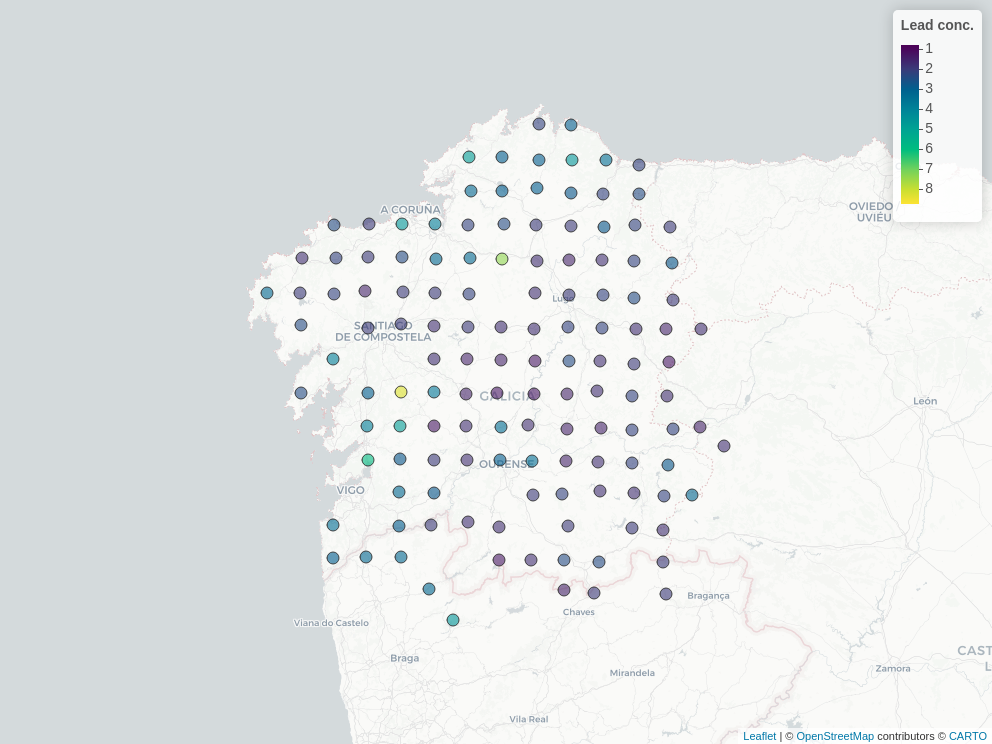
\includegraphics[width=3.31in,height=\textheight,keepaspectratio]{figures/galicia_ch1.png}

}

\caption{\label{fig-galicia-ch1}Data on the measured lead concentration
(in micrograms per gram dry weight) in moss samples collected in
Galicia, North-West of Spain.}

\end{figure}%

Lead is a heavy metal that, at high concentrations, can cause chronic
damage to living organisms over prolonged periods. For this reason, its
distribution and sources require regular monitoring. A common approach
is to measure lead concentrations in plants, which act as bioindicators
of environmental contamination. The data considered here
(Figure~\ref{fig-galicia-ch1}) consist of measurements from 132 moss
samples collected in the year 2000 in and around Galicia, a region in
north-western Spain. One of the main objectives of the survey was to map
the spatial distribution of lead concentration in order to identify
potential sources of contamination; for further details, see Fernández,
Rey, and Carballeira (2000).

Geostatistical modelling provides a framework for predicting lead
concentrations across Galicia and for distinguishing between random
variation, for instance due to measurement error, and genuine spatial
variation, which is the principal focus of analysis.

This dataset will be used throughout the book to illustrate the spatial
analysis of continuously measured variables using linear geostatistical
models.

\subsection{River-blindness in Liberia}\label{sec-rb-ch1}

\begin{figure}

\centering{

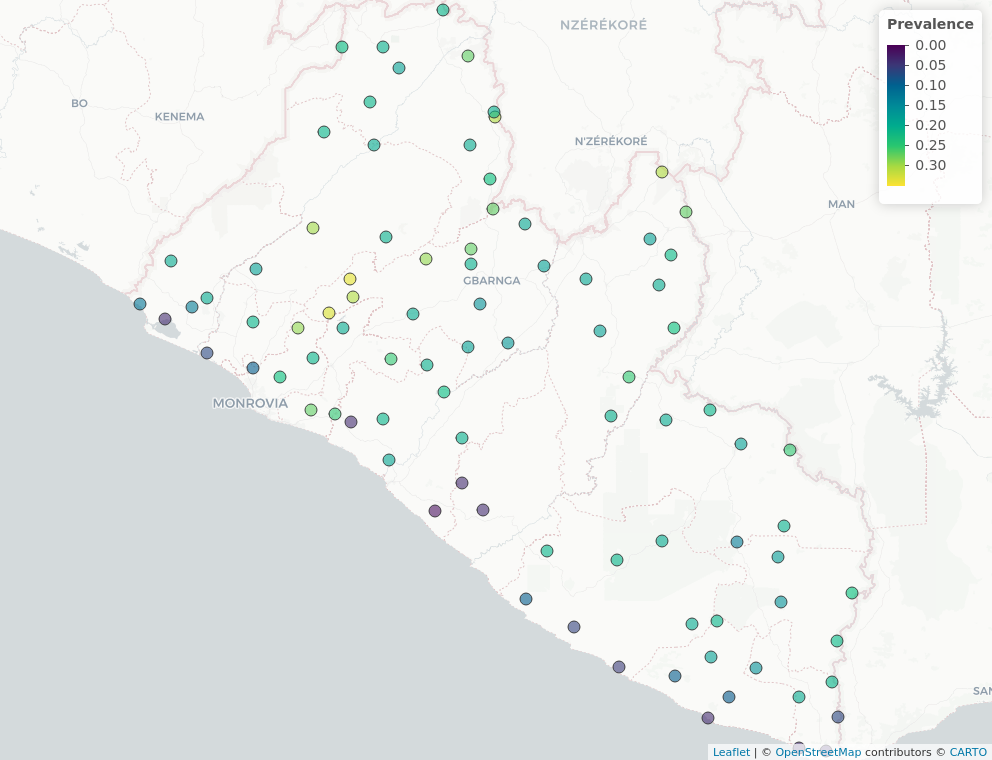
\includegraphics[width=3.31in,height=\textheight,keepaspectratio]{figures/liberia_ch1.png}

}

\caption{\label{fig-liberia-ch1}River-blindness data from a
cross-sectional survey carried out in Liberia.}

\end{figure}%

In low-resource settings, where disease registries are often absent,
cross-sectional surveys provide a critical tool for estimating disease
burden in the population of interest. The data considered in this
example (Figure~\ref{fig-liberia-ch1}) were collected as part of the
Rapid Epidemiological Mapping of Onchocerciasis (REMO), an Africa-wide
initiative conducted in 2011 across 20 countries (Zouré et al. 2014).
The purpose of REMO was to identify areas where river blindness
(onchocerciasis)---a parasitic disease transmitted by black flies that
breed along fast-flowing rivers---remains a public health problem. Of
particular concern are communities with prevalence above 20\%, which are
prioritised for treatment

In this book, we use data collected in Liberia to model nodule
prevalence, which measures the proportion of individuals in a population
presenting with palpable nodules under the skin. These nodules are
formed around adult \emph{Onchocerca volvulus} worms, the parasite
responsible for river blindness. Because detecting nodules through a
simple physical examination is far less costly and logistically
demanding than laboratory-based or molecular diagnostic methods, nodule
prevalence serves as a practical and widely used proxy for estimating
infection burden in large-scale epidemiological surveys, such as REMO.

Through this dataset, we demonstrate how to formulate and fit Binomial
geostatistical models and how these can be applied to predict prevalence
across a region of interest.

\subsection{Malaria in the Western Kenyan
Highlands}\label{sec-malaria-ch1}

\begin{figure}

\centering{

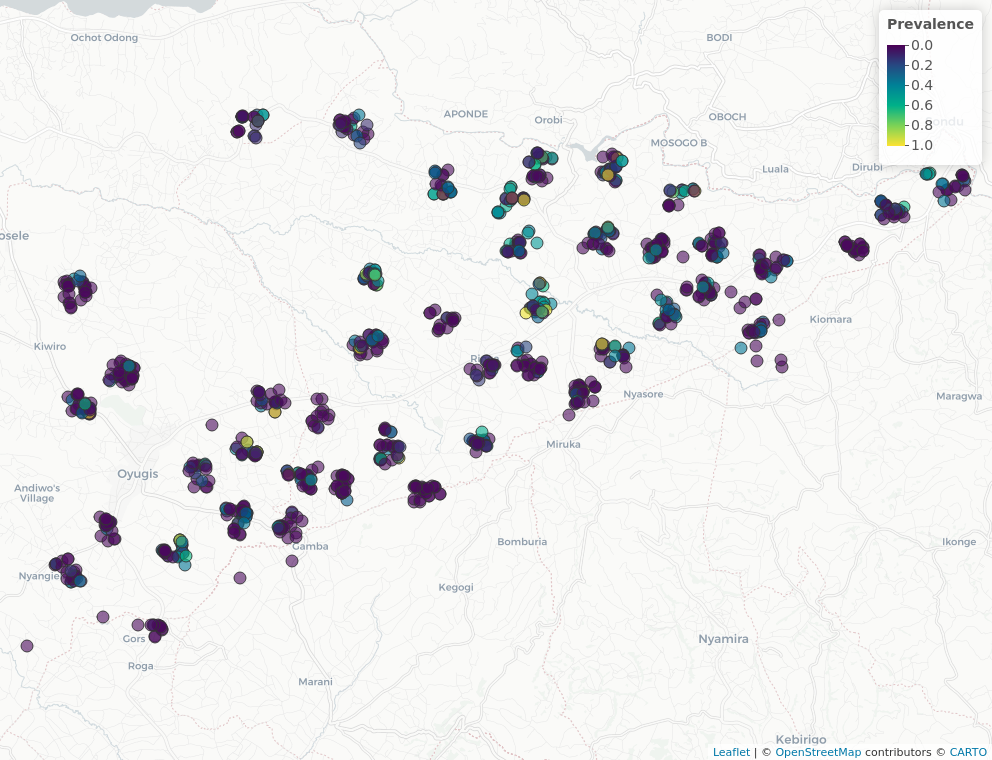
\includegraphics[width=3.31in,height=\textheight,keepaspectratio]{figures/malkenya_ch1.png}

}

\caption{\label{fig-malkenya-ch1}Malaria prevalence data from a
cross-sectional survey carried out in Nyanza Province, in the Western
Highlands of Kenya.}

\end{figure}%

Malaria is among the deadliest infectious diseases affecting populations
in tropical and subtropical regions. It is caused by parasites of the
genus \emph{Plasmodium}, transmitted through the bite of infected female
\emph{Anopheles} mosquitoes. In the following chapters, we analyse a
dataset (Figure~\ref{fig-malkenya-ch1}) from a cross-sectional community
survey conducted in July 2010 in Nyanza Province, in the western
highlands of Kenya (Stevenson 2013).

What distinguishes this dataset from the other examples is that it
contains both individual- and household-level information. The primary
outcome is the result of a rapid diagnostic test for malaria. In the
original study, data were collected from 46 community clusters (clearly
visible as spatial groupings in Figure~\ref{fig-malkenya-ch1}) each
defined by a primary school and the surrounding residential compounds
within approximately a 600 m radius. Each cluster therefore corresponds
to a school and its adjacent community catchment area.

In this book, we show how to incorporate the hierarchical structure of
the data together with the binary nature of the outcome at each stage of
the geostatistical analysis.

\subsection{\texorpdfstring{\emph{Anopheles gambiae} mosquitoes in
Southern
Cameroon}{Anopheles gambiae mosquitoes in Southern Cameroon}}\label{sec-mosq-data-ch1}

\begin{figure}

\centering{

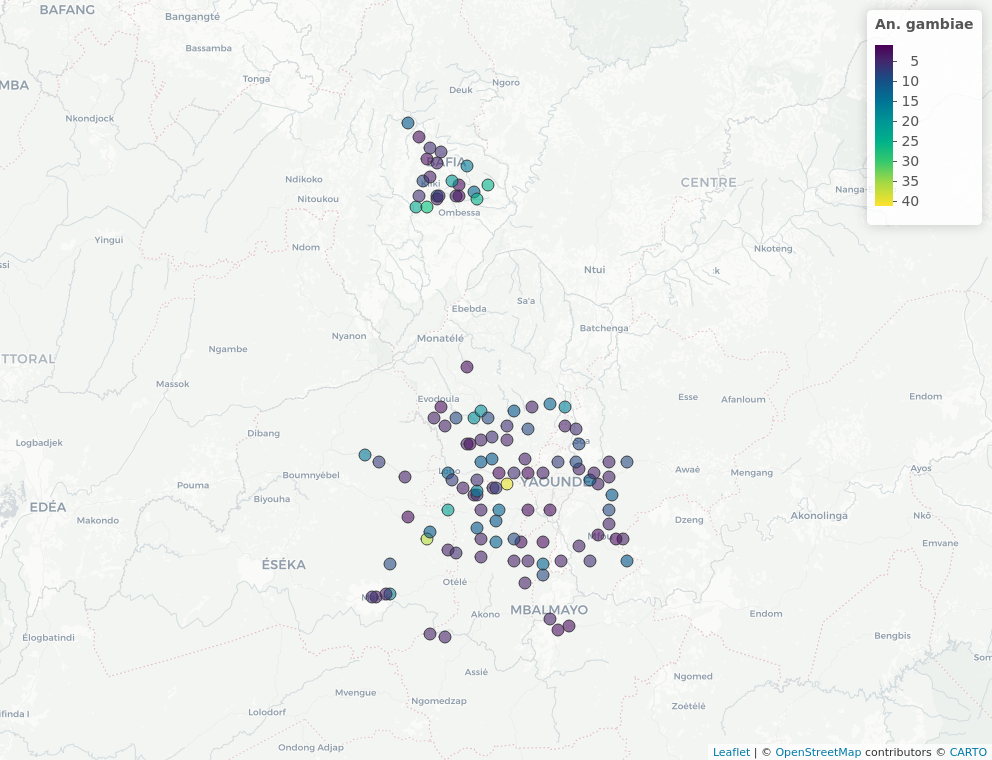
\includegraphics[width=3.31in,height=\textheight,keepaspectratio]{figures/anopheles_ch1.png}

}

\caption{\label{fig-anopheles-ch1}Map of the collected number of
\emph{Anopheles gambiae} mosquitoes in an area of Southern Cameroon.}

\end{figure}%

In studies of vector-borne and zoonotic diseases, understanding the
vector distribution can help to better guide the decision-making process
for the implementation, monitoring and evaluation of control programmes.
\emph{Anopheles gambiae} mosquitoes are one of the main vectors for
malaria transmission in sub-Saharan Africa. Their distribution over
space is affected by several environmental and climatic factors,
including temperature, humidity and vegetation.

The data-set on mosquitoes (Figure~\ref{fig-anopheles-ch1}) that we will
use in the book consists of a sub-set taken from a larger database (Tene
Fossog et al. 2015). This was assembled in order to understand how the
environment affects the distribution of different species of
\emph{Anopheles} mosquitoes in sub-Saharan Africa. This example data-set
will be used to illustrate the application of Poisson geostatistical
models for mapping mosquitoes abundance.

\subsection{Simulated-dataset}\label{sec-italy-sim-data-ch1}

\begin{figure}

\centering{

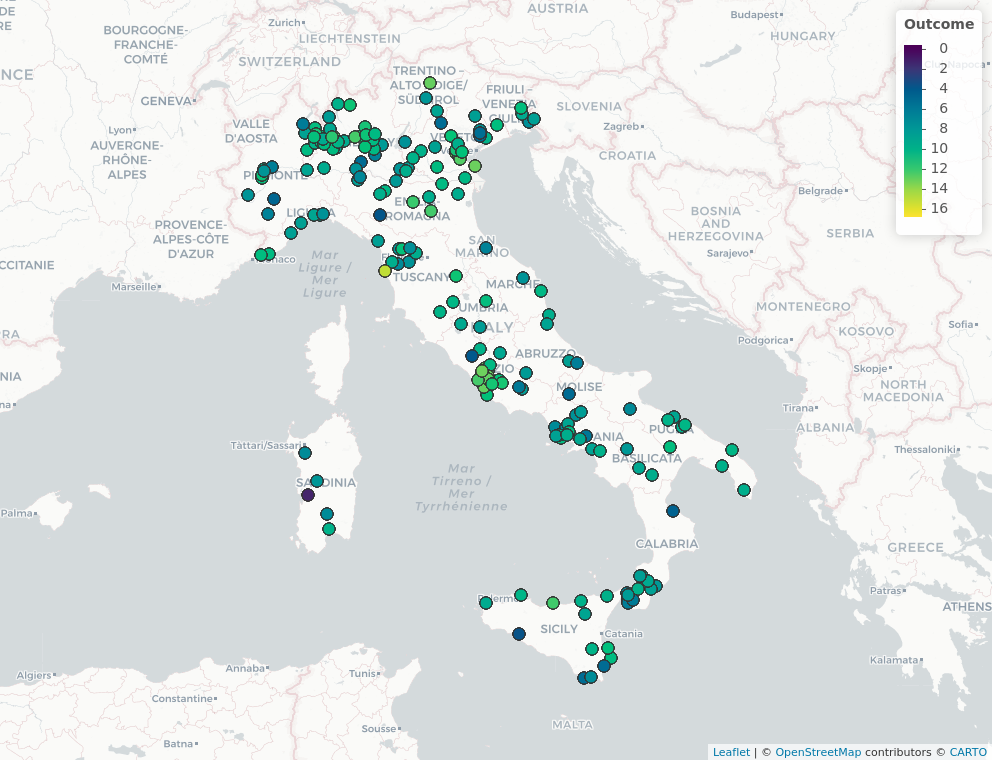
\includegraphics[width=3.31in,height=\textheight,keepaspectratio]{figures/italy_sim_ch1.png}

}

\caption{\label{fig-italy-sim-ch1}Map of the locations of the simulated
data-set generated over Italy for a continuous outcome.}

\end{figure}%

The data-set reported in Figure~\ref{fig-italy-sim-ch1} was generated
using a geostatistical model, with the addition of unstructured random
effects at provincial and regional level. More details on how this
data-set was generated will be provided in
Section~\ref{sec-linear-model}. Whilst this data-set does not have any
scientific relevance, it will serve us to illustrate some of the more
advanced features of the \texttt{RiskMap} package that enable the
inclusion of random effects, in addition to the latent Gaussian process
that is common to all geostatistical models. The skills you will acquire
through the analysis of this data-set will be useful for the analysis of
data-sets presented as case studies in Chapter~\ref{sec-case-studies}.

\section{Geostatistical problems and geostatistical
models}\label{sec-geostat-models}

What the examples of the previous section have in common is that, in
each case, the goal of the statistical analysis is to draw inferences on
an unobserved spatially continuous surface using data collected from a
finite set of locations. The lead concentration in Galicia, the
prevalence for river-blindness in Liberia and the abundance of \emph{A.
gambiae} mosquitoes in Cameroon can all be represented as spatially
continuous processes that originate from the combined effects of
environmental factors. We denote this class of inferential problems as
\emph{geostatistical problems} for which a solution can be found through
the development and application of suitable \emph{geostatistical
models}, which are the subject of this book.

As one can soon realize, geostatistical problems are not unique to
global health but arise in many other fields of science, including
economics, physics, biology and geology. It thus comes to no surprise
that geostatistics was initially developed in the South African mining
industry in the 1950s (Krige 1951). This was then further developed as a
self-contained discipline by Georges Matheron and other researchers at
Fontainebleau, in France (Matheron 1963; Chilès and Delfiner 2016). In
Watson (1971) and Watson (1972) a first connection is drawn between
geostatistics and the prediction of stochastic processes. However, it is
only with Ripley (1981) and then N. A. C. Cressie (1991) that
geostatistics is explicitly brought into a classical statistical
framework for the analysis of spatially referenced data. P. J. Diggle,
Tawn, and Moyeed (1998) coined the term \emph{model-based geostatistics}
and introduced this as belonging to the general class of generalized
linear mixed models (Breslow and Clayton 1993), while emphasizing the
use of likelihood-based methods of inference. As in P. J. Diggle, Tawn,
and Moyeed (1998), also in this book, we advocate the application of
model-based geostatistical models as a class of parametric statistical
models on which inference can be carried out using either maximum
likelihood estimation or Bayesian methods.

More precisely, our attention will be directed at the class of
\emph{generalized linear geostatistical models}, or GLGMs. To formally
specify this, we define the spatial stochastic process \(S(\cdot)\),
representing an unobserved spatially continuous random field. For a set
of locations \(X = (x_1, \ldots, x_n)\), we denote by

\[
S = (S(x_1), \ldots, S(x_n))
\]

the vector of process realizations at those locations. We also define
the random vector \(Y = (Y_1, \ldots, Y_n)\), representing the outcomes
observed at the same locations. Throughout, we use \([A]\) to denote
``the distribution of the random variable \(A\).'' To formulate a GLGM,
we should then specify the joint distribution of \(S\) and \(Y\), which
we write as

\begin{equation}\phantomsection\label{eq-glgm-joint-ch1}{
[Y, S] = [S] [Y | S].
}\end{equation}

On the right-hand side of the equation above, we have factorized the
joint distribution of \(Y\) and \(S\), as the product between the
marginal distribution of \(S\) and the conditional distribution of \(Y\)
given \(S\). Hence, the formulation of a GLGM can be broken down into
the tasks of formulating \([S]\) and \([Y | S]\).

In defining \([S]\), throughout the book, we shall assume that this is a
zero-mean stationary and isotropic Gaussian process. In other words,
these assumptions impose that the joint distribution of
\(S(X) = (S(x_1),\ldots,S(x_n))\), i.e.~the process \(S\) at the sampled
locations \(x_1, \ldots, x_n\), is invariant with respect to rotations
and translations of the locations \(X\). In practical terms, the main
implication of this is that, for any pair of locations \(x_i\) and
\(x_j\) the correlation function \(\rho(\cdot)\) between \(S(x_i)\) and
\(S(x_j)\) is purely a function of the Euclidean distance, \(u_{ij}\),
between \(x_i\) and \(x_j\),
i.e.~\begin{equation}\phantomsection\label{eq-correlation-ch1}{
{\rm cov}\{S(x_i), S(x_j)\} = \sigma^2\rho(u_{ij}),
}\end{equation}

where \(\sigma^2\) is the variance of \(S(x)\) for all \(x\). Below we
provide more details on the type of covariance functions that we
consider in this book. Furthermore, the fact that we assume the process
\(S\) to have mean zero is because this process acts as a residual term
in our modelling of \(Y\). This aspect will be reiterated several times
in the following chapters, as it has important implications for the
interpretation of the other components of a geostatistical model, and
for understanding the results of the analysis.

Finally, we model \([Y | S]\), i.e.~the distribution of \(Y\) given
\(S\), as a set of mutually independent distributions which belong to
the exponential family, as defined in classical generalized linear
modelling framework (Nelder and Wedderburn 1972). It then follows that,
we can write \([Y | S]\) as

\begin{equation}\phantomsection\label{eq-glm-ch1}{
[Y | S] = \prod_{i=1}^n [Y_i | S(x_i)].
}\end{equation}

The final step then consists of specifying a distribution for
\([Y_i | S(x_i)]\). Table~\ref{tbl-glm} gives the range, mean and
variance of the three specifications for \([Y_i | S(x_i)]\) which we
will consider in this book. In Table~\ref{tbl-glm}, the \emph{canonical
function}, say \(g(\cdot)\), denotes the natural transformation of the
mean component \(\mu_i\) that allows us to introduce both covariates and
the spatial process \(S(x_i)\) into the model so as to explain the
variation in \(\mu_i\) as

\begin{equation}\phantomsection\label{eq-linear-predictor-ch1}{
g(\mu_i) = d(x_i)^\top \beta + S(x_i).
}\end{equation}

where \(d(x_i)\) is a vector of spatially referenced covariates with
associated regression coefficients \(\beta\). Finally, the quantity
\(m_i\), which appears in the formulation of the Binomial and Poisson
distributions, is an offset quantity that accounts for the number of
\emph{tests} or the population size at a given location \(x_i\).

\begin{longtable}[]{@{}
  >{\raggedright\arraybackslash}p{(\linewidth - 8\tabcolsep) * \real{0.2000}}
  >{\raggedright\arraybackslash}p{(\linewidth - 8\tabcolsep) * \real{0.2000}}
  >{\raggedright\arraybackslash}p{(\linewidth - 8\tabcolsep) * \real{0.2000}}
  >{\raggedright\arraybackslash}p{(\linewidth - 8\tabcolsep) * \real{0.2000}}
  >{\raggedright\arraybackslash}p{(\linewidth - 8\tabcolsep) * \real{0.2000}}@{}}
\caption{Type of outcomes \(Y_{i}\) considered in this
book.}\label{tbl-glm}\tabularnewline
\toprule\noalign{}
\begin{minipage}[b]{\linewidth}\raggedright
Distribution
\end{minipage} & \begin{minipage}[b]{\linewidth}\raggedright
Range of \(Y_i\)
\end{minipage} & \begin{minipage}[b]{\linewidth}\raggedright
Mean of \([Y_i | S(x_i)]\)
\end{minipage} & \begin{minipage}[b]{\linewidth}\raggedright
Variance of \([Y_i | S(x_i)]\)
\end{minipage} & \begin{minipage}[b]{\linewidth}\raggedright
Canonical link
\end{minipage} \\
\midrule\noalign{}
\endfirsthead
\toprule\noalign{}
\begin{minipage}[b]{\linewidth}\raggedright
Distribution
\end{minipage} & \begin{minipage}[b]{\linewidth}\raggedright
Range of \(Y_i\)
\end{minipage} & \begin{minipage}[b]{\linewidth}\raggedright
Mean of \([Y_i | S(x_i)]\)
\end{minipage} & \begin{minipage}[b]{\linewidth}\raggedright
Variance of \([Y_i | S(x_i)]\)
\end{minipage} & \begin{minipage}[b]{\linewidth}\raggedright
Canonical link
\end{minipage} \\
\midrule\noalign{}
\endhead
\bottomrule\noalign{}
\endlastfoot
Gaussian & \((-\infty, +\infty)\) & \(\mu_i\) & \(\tau^2\) &
\(g(\mu_i) = \mu_i\) \\
Binomial & \(1,\dots,m_i\) & \(m_i\mu_i\) & \(m_i\mu_i(1-\mu_i)\) &
\(g(\mu_i) = \log\{ \mu_i/(1-\mu_i) \}\) \\
Poisson & \(1,2,\ldots,\infty\) & \(m_i\mu_i\) & \(m_i\mu_i\) &
\(g(\mu_i) = \log\{ \mu_i \}\) \\
\end{longtable}

Based on the formulation in (\ref{eq-linear-predictor-ch1}), we can see
that \(S(x_i)\) quantifies residual spatial effects on \(\mu_i\) that
have not been accounted for by the covariates \(d(x_i)\). In an ideal
scenario, the covariates \(d(x_i)\) should explain all the spatial
variation without the need for \(S(x_i)\). Although this is often
unrealistic, in practice we may be able to explain most of the variation
in \(\mu_i\) through \(d(x_i)\) and, hence, reduce \(S(x_i)\) to a
negligible component. In Chapter 2, we will show how a thorough
exploratory analysis can help to understand whether we have come close
to that ideal scenario or if we need to use a GLGM to model the data.

The model described in (\ref{eq-linear-predictor-ch1}) can be seen as
the most basic GLGM that can be used for a geostatistical analysis. As
we will see in the analysis of some of the examples, extensions of this
model will be required to accommodate the intrinsic non-spatial random
variation of the data which is not captured by the covariates.

Statistical models are typically applied in two main ways: to make
predictions, or to model associations that help us understand
relationships between variables, whether causal or not. Most
geostatistical applications fall into the first category, where the
objective is to make predictive inferences about the process \(S(x)\) at
locations \(x\) that are typically outside the set of sampled sites.
However, as we will illustrate in later chapters, geostatistical models
also play an important role in understanding associations between
variables. In particular, we will show that accounting for spatial
correlation can substantially affect both the point estimates and
standard errors of the regression parameters \(\beta\).

\subsection{The Matern family of correlation
functions}\label{sec-matern-correlation}

Throughout the book, we shall consider the Matern (2013) family of
correlation functions to model the spatial correlation of the Gaussian
process \(S(x)\). This is defined as

\begin{equation}\phantomsection\label{eq-matern}{
\rho(u;\phi,\kappa) = \{2^{\kappa-1} \Gamma(\kappa)\}^{-1} (u/\phi)^\kappa K_\kappa(u/\phi),
}\end{equation}

where \(\phi>0\) and \(\kappa>0\) are parameters and \(K_\kappa(\cdot)\)
is the modified Bessel function of the third kind of order \(\kappa\).
The parameters \(\phi\) and \(\kappa\) regulate how fast the spatial
correlation decays to zero with increasing distance, and the
\emph{smoothness} of the process, respectively. By smoothness we mean
the degree of differentiability of the underlying spatial surface:
smaller values of \(\kappa\) produce rougher, less regular surfaces,
whereas larger values of \(\kappa\) lead to smoother and more spatially
continuous processes.

A special case of the Matern family of correlation functions, obtained
when \(\kappa = 0.5\), will be of particular relevance to the
applications considered in this book. This is the exponential
correlation function, which we write as

\begin{equation}\phantomsection\label{eq-exp}{
\rho(u;\phi) = \exp\{-u/\phi\}.
}\end{equation}

Another special case, which we do not consider in this book but which is
often used in machine learning applications, is the Gaussian correlation
function, obtained as a limiting case for \(\kappa \to +\infty\),
representing the smoothest possible process within the Matérn family.

To better understand how \(\phi\) and \(\kappa\) affect the spatial
correlation and the pattern of the spatial surface, we now consider some
examples.

\begin{figure}

\centering{

\pandocbounded{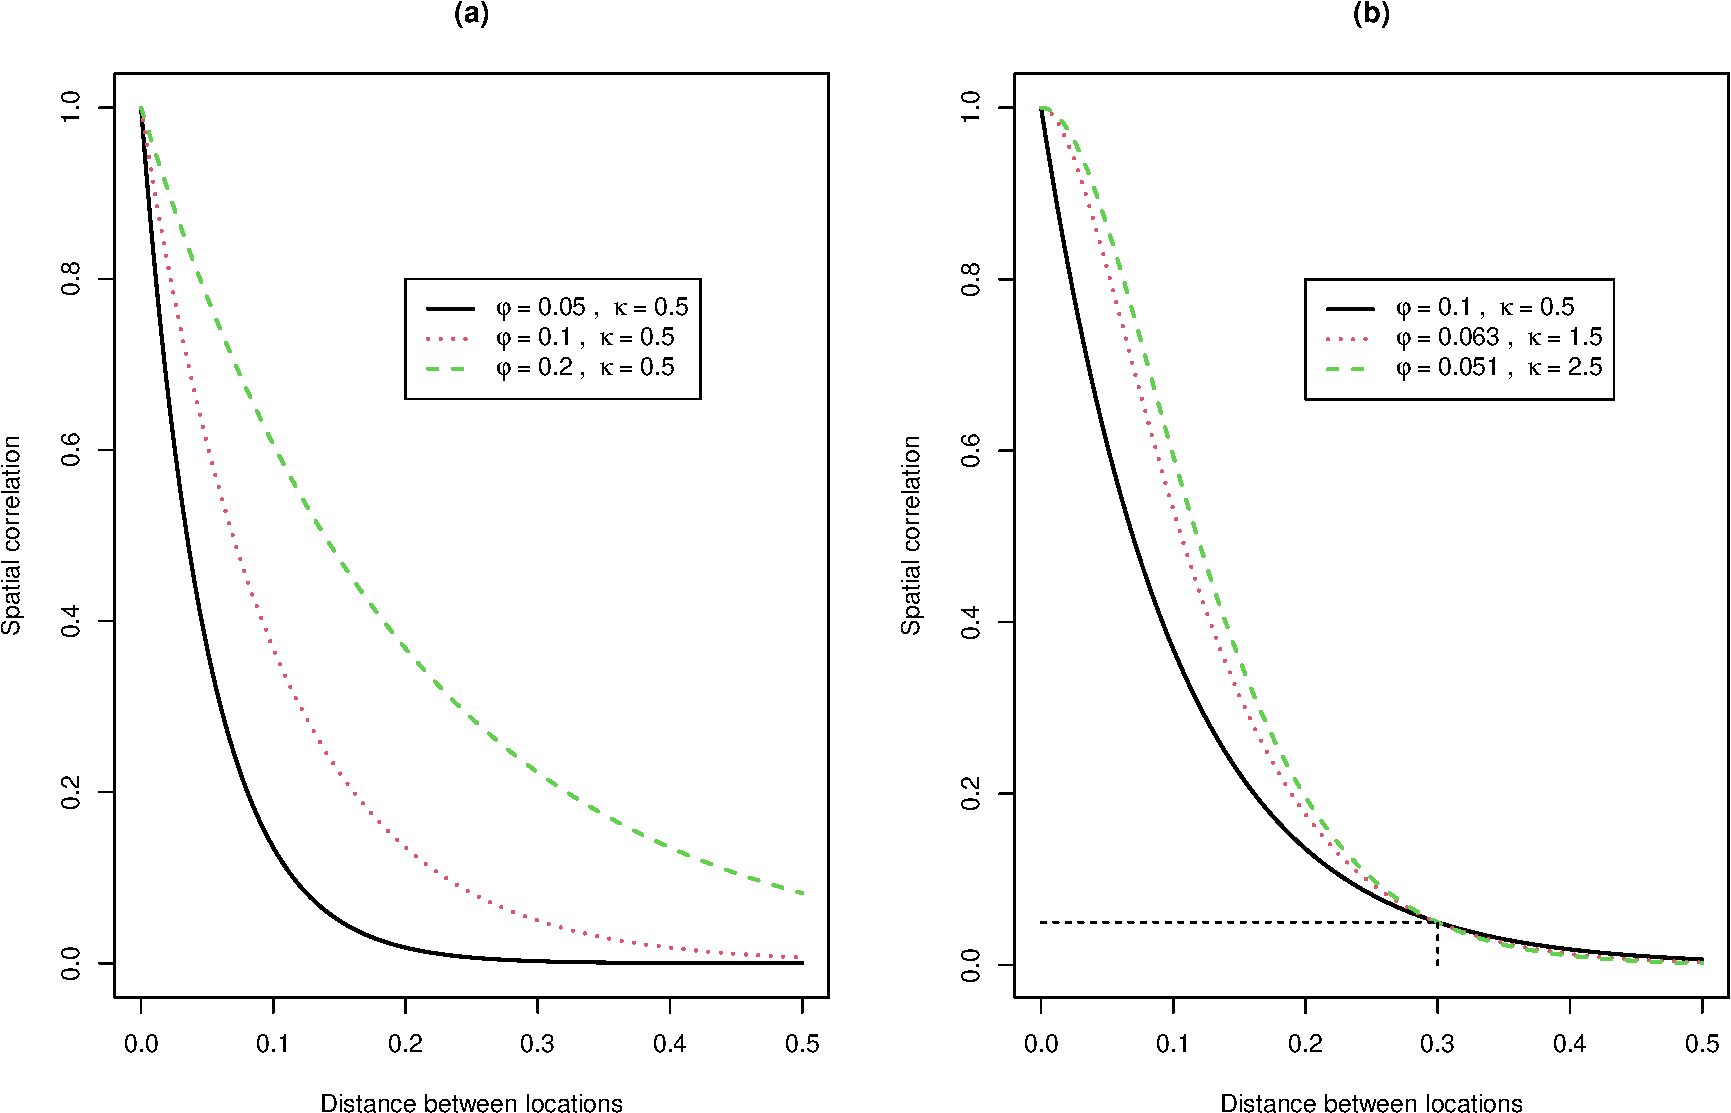
\includegraphics[keepaspectratio]{01_intro_files/figure-pdf/fig-matern-func-1.pdf}}

}

\caption{\label{fig-matern-func}Examples of stationary and isotropic
Matern correlation functions. Panel (a) shows three different
correlation functions that have the same smoothness parameter of
\(\kappa=0.5\), while varying the scale parameter \(\phi\) over
\({0.05, 0.1, 0.2}\). In panel (b) the scale of the spatial correlation
\(\phi\) is chosen so that each of the three functions reaches 0.05 at
distance 0.3 (as also shown by the horizontal and vertical black dashed
segments).}

\end{figure}%

Figure~\ref{fig-matern-func} shows six different Matern correlation
functions. In panel (a), we have kept \(\kappa\) fixed to 0.5 and varied
\(\phi\) over the values 0.05, 0.1 and 0.2. For larger values of
\(\phi\) the correlation function has a slower decay to zero. Panels (a)
to (c), in Figure~\ref{fig-matern-sim}, show three realizations of a
Gaussian process from each of these correlation functions. The mean of
the Gaussian process was set to zero and variance to 1. We can observe
that spatial correlations with larger scales are associated with longer
spatial trends, whilst smaller scales exhibit a patchier pattern. This
is because, as \(\phi\) takes values that are closer to zero, the
spatial surface will tend to show a less structured pattern and will
revert towards its zero mean more rapidly. In our examples in the book,
we will often use the so called \emph{practical range} to interpret our
estimates for \(\phi\). The practical range is defined as the distance
at which spatial correlation reaches 0.05, hence one can interpret this
as the distance beyond which observations can be considered
approximately independent. In the case of the exponential correlation
function, the practical range is
\(\log(20) \times \phi \approx 3 \phi\).

Finally, let us consider the correlation functions shown in panel (b) of
Figure~\ref{fig-matern-func}. Here, we vary \(\kappa\) over the values
0.5, 1.5, and 2.5, while keeping \(\phi\) fixed so that all three
correlation functions reach 0.05 at a distance of 0.3. This setup allows
us to isolate the effect of \(\kappa\) on the \emph{smoothness} of the
spatial process, while maintaining approximately the same correlation
range across the three cases.

In Figure~\ref{fig-matern-sim}, we show three realizations from these
correlation functions. We notice that smaller values of \(\kappa\)
(e.g., \(\kappa = 0.5\)) produce rougher and less regular spatial
patterns, whereas larger values (e.g., \(\kappa = 2.5\)) result in
smoother and more continuous surfaces. These visual differences reflect
the varying degrees of \emph{differentiability} of the Gaussian process,
which mathematically determines its local behavior and hence its
smoothness.

Readers interested in the theoretical foundations of these properties
may refer to Chapter 2 of Stein (1999).

\begin{figure}

\centering{

\pandocbounded{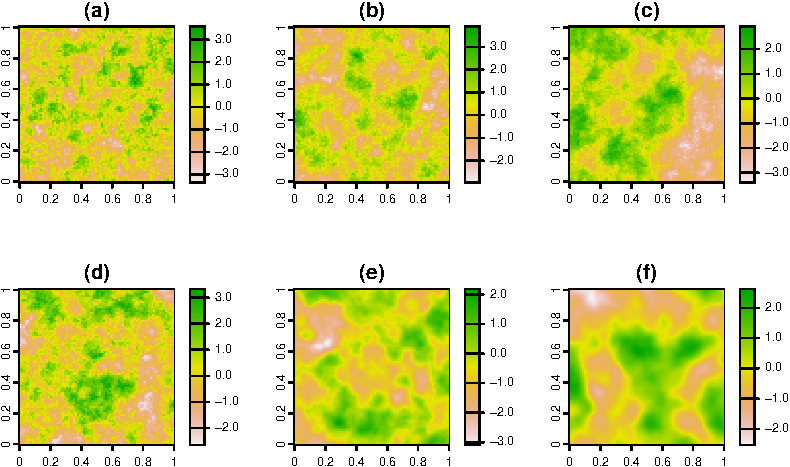
\includegraphics[keepaspectratio]{01_intro_files/figure-pdf/fig-matern-sim-1.pdf}}

}

\caption{\label{fig-matern-sim}Simulated spatial surface using the three
correlation functions shown in Figure~\ref{fig-matern-func}. Panels (a),
(b) and (c) correspond to the correlation functions from panel (a) in
Figure~\ref{fig-matern-func} and in order these are: \(\phi = 0.05\) and
\(\kappa=0.5\); (b) \(\phi=0.1\) and \(\kappa=0.5\); (c) \(\phi=0.2\)
and \(\kappa=0.5\). Panels (c), (d) and (e) correspond to the
correlation functions from panel (b) in Figure~\ref{fig-matern-func} and
in order these are: \(\phi = 0.1\) and \(\kappa=0.5\); (b)
\(\phi=0.063\) and \(\kappa=1.5\); (c) \(\phi=0.051\) and
\(\kappa=2.5\).}

\end{figure}%

The flexibility provided by the Matern correlation function in capturing
different forms of spatial correlations has made it the most widely used
correlation function in model-based geostatistics (Stein 1999). For this
reason, in this book we will consider the Matern correlation function.
We will consider estimation issues related to the Matern correlation in
Chapter~\ref{sec-estimation}.

\section{Workflow of a statistical analysis and structure of the
book}\label{sec-workflow}

\begin{figure}

\centering{

\pandocbounded{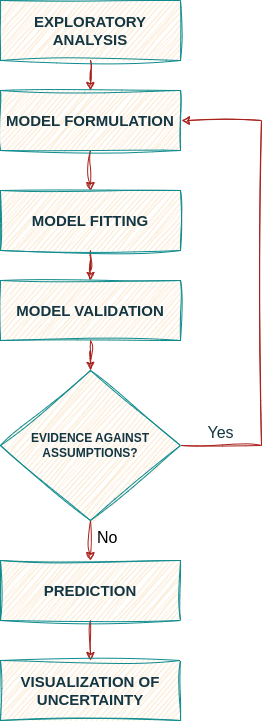
\includegraphics[keepaspectratio]{figures/workflow_diagram.png}}

}

\caption{\label{fig-stages}Stages of a statistical analysis}

\end{figure}%

Figure~\ref{fig-stages} illustrates the stages involved in carrying out
a geostatistical analysis of the examples introduced in
Section~\ref{sec-examples-ch1}. The process begins with exploratory data
analysis, which is essential for understanding the empirical
associations between risk factors and the health outcome of interest. In
our case, this stage also helps justify the use of geostatistical models
by questioning the assumptions underlying standard generalized linear
models. The insights gained from this initial step guide the formulation
of a suitable statistical model, whose parameters are then estimated
using likelihood-based methods. This approach provides measures of
uncertainty not only for the regression coefficients but also for the
parameters that define the structure of spatial correlation in the data.

Once estimation has been carried out, the next step is model validation,
where diagnostic tools are used to assess whether the fitted model can
be trusted to represent the observed variation in the outcome. If the
diagnostics indicate a poor fit, the process returns to the formulation
stage to address the shortcomings revealed by the validation. If no
evidence against the model is found, we move on to spatial prediction.

At this stage, defining appropriate predictive targets is crucial, as
they ensure that the analysis answers the original research questions
and supports decision making. An equally important component is
evaluating how well the model predicts unobserved data, often referred
to as predictive performance. In geostatistical applications, this
evaluation is particularly challenging because spatial data are
typically sparse and irregularly distributed. A widely used approach to
quantify predictive performance is cross validation, which involves
withholding a subset of observations, fitting the model to the remaining
data, and then comparing the predictions to the held out observations.
The design and interpretation of cross validation, however, depend on
the ultimate goal of the analysis, for example whether the aim is to
make predictions within the study region or to extrapolate beyond the
sampled area. In addition to cross validation, simulation studies
provide a valuable complementary tool, allowing us to better understand
how a model should be expected to perform on average and to assess
whether the results from a given analysis are consistent with this
expected behaviour.

In the remainder of this book, each chapter focuses on one or more of
these stages as shown in Figure~\ref{fig-stages}.
Chapter~\ref{sec-handling-data} introduces methods for working with
spatial data in R, with a focus on raster and vector formats, including
points and polygons. The skills developed in this chapter are applied
throughout the book and are especially important in
Chapter~\ref{sec-geo-prediction} and Chapter~\ref{sec-case-studies},
where predictive maps of health outcomes are generated.
Chapter~\ref{sec-estimation} then describes the process of model
formulation and estimation, showing how exploratory analyses inform the
choice of model and how maximum likelihood methods can be used for
parameter estimation. Chapter~\ref{sec-geo-prediction} builds on this by
demonstrating how fitted models can be used for spatial prediction on
both continuous and aggregated scales, and how predictive performance
can be assessed to identify the most suitable model. Finally,
Chapter~\ref{sec-case-studies} presents complete applications of all
methods to three datasets, summarizing the full geostatistical workflow
and illustrating additional features of the \texttt{RiskMap} R package
not covered in earlier chapters.

\bookmarksetup{startatroot}

\chapter{Handling of spatial data in R}\label{sec-handling-data}

\section{Introduction}\label{introduction-1}

Geostatistical analysis primarily deals with \textbf{point-referenced
data}. However, geostatistical modeling often requires more than just
point data, \textbf{raster} and \textbf{areal (polygon)} data are
frequently used to build essential covariates, enhance spatial
understanding, or provide environmental context. For instance,
population density, climate data, land use, and elevation, often key
covariates in many spatial analyses, usually come in raster or polygon
formats. Efficient handling of these different data types is critical
for successful model-building. This chapter provides a comprehensive
guide to the various stages of managing spatial data in R, using the
\texttt{sf} and \texttt{terra} packages, to support a complete
geostatistical workflow.

\section{Spatial data handling in geostatistical
analysis}\label{spatial-data-handling-in-geostatistical-analysis}

Throughout a geostatistical analysis, handling spatial data takes place
at multiple key stages:

\begin{enumerate}
\def\labelenumi{\arabic{enumi}.}
\item
  \textbf{Retrieving External Spatial Data Sources}: Before starting the
  modeling process, one often needs to acquire spatial datasets from
  external sources to improve model accuracy. These could include
  satellite-derived environmental variables, population data from
  \href{https://www.worldpop.org/}{WorldPop}, or climate data from
  \href{https://www.worldclim.org/}{WorldClim}. Acquiring these datasets
  and ensuring they are in compatible formats and resolutions is an
  essential early step in spatial analysis.
\item
  \textbf{Importing and Standardizing Spatial Data}: Once external data
  is obtained, it must be imported into R. This involves handling
  various file formats such as shapefiles or geopackages for vector data
  and GeoTIFFs for raster data. Moreover, different datasets might use
  different \textbf{Coordinate Reference Systems (CRS)}, requiring CRS
  standardization to ensure that all datasets align correctly. Failure
  to standardize CRS can result in spatial misalignments and incorrect
  results.
\item
  \textbf{Extracting Covariate Information for Modeling}: Covariate
  extraction is an essential step in geostatistical modeling. After
  importing spatial data, it is necessary to extract relevant covariate
  information both for the \textbf{sampled locations} (where we have
  observed data) and the \textbf{prediction locations} (where we wish to
  make predictions). This step involves linking raster or polygonal
  covariates, such as climate, population, or land cover data, to the
  geostatistical data points.
\item
  \textbf{Prediction and Creation of a Spatial Grid}: For predictive
  geostatistical models, a regular grid of points is often created over
  the study region. Covariates must then be assigned to each grid point
  to make predictions across the entire region of interest. Creating
  predictive grids and linking them to the necessary covariates is key
  to generating continuous spatial predictions from geostatistical
  models.
\item
  \textbf{Visualizing Spatial Data}: Visualization is crucial for
  exploring spatial data, interpreting model results, and communicating
  findings. Whether working with point-referenced data, polygons, or
  rasters, clear and effective visualization helps reveal patterns that
  inform the modeling process. Effective visualization can also help
  highlight covariate trends, spatial clusters, and uncertainty in
  predictions.
\end{enumerate}

\section{Accessing covariates for disease
mapping}\label{accessing-covariates-for-disease-mapping}

Covariates can play a crucial role in understanding and modeling the
spatial variation in disease risk. In geostatistical analysis,
incorporating environmental, demographic, and climatic variables might
improve the predictive power of models or at least reduce the level of
uncertainty in the predictions. These covariates can influence factors
such as the spread of infectious diseases, the distribution of disease
vectors, and the socio-economic conditions that impact health outcomes.

A wide range of open-access spatial datasets provide covariates for
disease mapping. These include population density, climate, land cover,
and human infrastructure data, which often come in raster or polygon
formats. Alongside these environmental covariates, administrative
boundaries are also crucial for public health analysis, as they help
organize and aggregate data at different levels (e.g., country, region,
or district). For example, aggregating health outcomes or covariate data
by administrative units allows researchers to identify geographic
disparities and allocate resources accordingly. Fortunately, open-source
platforms such as \href{https://www.geoboundaries.org/}{geoBoundaries}
provide easily accessible administrative boundary data for many
countries at various levels of granularity. This data is available in
formats compatible with geospatial analysis tools in R, making it easy
to integrate into geostatistical workflows.

Table~\ref{tbl-data-sources} below summarizes key sources of covariates
useful in disease mapping. Each dataset offers specific types of data,
from satellite-derived environmental variables to gridded population
estimates and administrative boundaries, which can be accessed through
various R packages or APIs.

\begin{longtable}[]{@{}
  >{\raggedright\arraybackslash}p{(\linewidth - 6\tabcolsep) * \real{0.1984}}
  >{\raggedright\arraybackslash}p{(\linewidth - 6\tabcolsep) * \real{0.2619}}
  >{\raggedright\arraybackslash}p{(\linewidth - 6\tabcolsep) * \real{0.3651}}
  >{\raggedright\arraybackslash}p{(\linewidth - 6\tabcolsep) * \real{0.1746}}@{}}
\caption{Some key sources of covariates useful in disease mapping and R
packages to retrieve them.}\label{tbl-data-sources}\tabularnewline
\toprule\noalign{}
\begin{minipage}[b]{\linewidth}\raggedright
\textbf{Source}
\end{minipage} & \begin{minipage}[b]{\linewidth}\raggedright
\textbf{Data Type}
\end{minipage} & \begin{minipage}[b]{\linewidth}\raggedright
\textbf{Description}
\end{minipage} & \begin{minipage}[b]{\linewidth}\raggedright
\textbf{R Package}
\end{minipage} \\
\midrule\noalign{}
\endfirsthead
\toprule\noalign{}
\begin{minipage}[b]{\linewidth}\raggedright
\textbf{Source}
\end{minipage} & \begin{minipage}[b]{\linewidth}\raggedright
\textbf{Data Type}
\end{minipage} & \begin{minipage}[b]{\linewidth}\raggedright
\textbf{Description}
\end{minipage} & \begin{minipage}[b]{\linewidth}\raggedright
\textbf{R Package}
\end{minipage} \\
\midrule\noalign{}
\endhead
\bottomrule\noalign{}
\endlastfoot
\textbf{WorldClim} & Climate (temperature, rainfall) & Global climate
data & \texttt{geodata} \\
\textbf{MODIS} & Remote Sensing & Satellite imagery (e.g., vegetation
indices) & \texttt{MODIStsp} \\
\textbf{OpenStreetMap (OSM)} & Human settlements, roads & Global
geographic features & \texttt{osmdata} \\
\textbf{Google Earth Engine} & Satellite imagery & Large-scale
environmental data analysis & \texttt{rgee} \\
\textbf{WorldPop} & Population data & Gridded population density
estimates & \texttt{wpgpDownloadR} \\
\end{longtable}

\subsection{Example: Downloading administrative
boundaries}\label{example-downloading-administrative-boundaries}

Administrative boundaries provide an essential spatial structure for
many types of geostatistical analyses, particularly in disease mapping
where data is often aggregated by administrative units such as regions,
districsts or provinces. The
\href{https://www.geoboundaries.org/}{geoBoundaries} datasets, which are
accessible via the \texttt{rgeoboundaries} package, provide openly
available administrative boundary data for nearly every country,
allowing researchers to integrate these boundaries into their analyses
seamlessly.

\begin{Shaded}
\begin{Highlighting}[]
\FunctionTok{par}\NormalTok{(}\AttributeTok{mar =} \FunctionTok{c}\NormalTok{(}\DecValTok{0}\NormalTok{, }\DecValTok{0}\NormalTok{, }\DecValTok{0}\NormalTok{, }\DecValTok{0}\NormalTok{))  }\CommentTok{\#| hide\_line}
\CommentTok{\# Load the rgeoboundaries package}
\FunctionTok{library}\NormalTok{(rgeoboundaries)}

\CommentTok{\# Download administrative boundaries for Liberia (level 0: country)}
\NormalTok{liberia\_admin0 }\OtherTok{\textless{}{-}} \FunctionTok{gb\_adm0}\NormalTok{(}\StringTok{"Liberia"}\NormalTok{)}

\CommentTok{\# Do the same for level 1: regions}
\NormalTok{liberia\_admin1 }\OtherTok{\textless{}{-}} \FunctionTok{gb\_adm1}\NormalTok{(}\StringTok{"Liberia"}\NormalTok{)}

\CommentTok{\# Plot the administrative boundaries}
\FunctionTok{plot}\NormalTok{(liberia\_admin0}\SpecialCharTok{$}\NormalTok{geometry)}
\FunctionTok{plot}\NormalTok{(liberia\_admin1}\SpecialCharTok{$}\NormalTok{geometry)}
\end{Highlighting}
\end{Shaded}

\begin{figure}

\begin{minipage}{0.50\linewidth}

\centering{

\pandocbounded{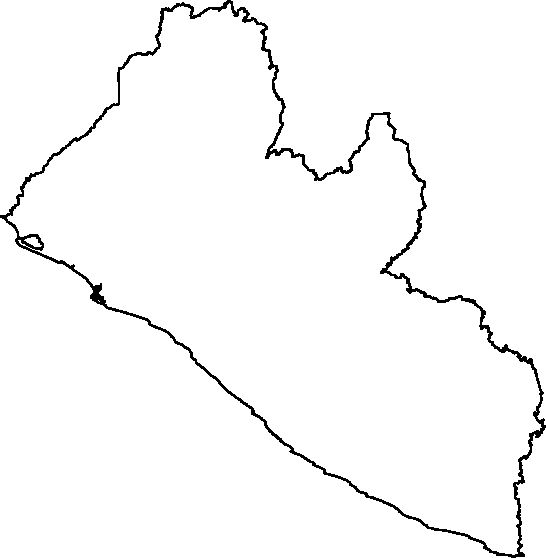
\includegraphics[keepaspectratio]{02_handling-spatial-data_files/figure-pdf/fig-liberia-admin-1.pdf}}

}

\subcaption{\label{fig-liberia-admin-1}Adimin level 0}

\end{minipage}%
%
\begin{minipage}{0.50\linewidth}

\centering{

\pandocbounded{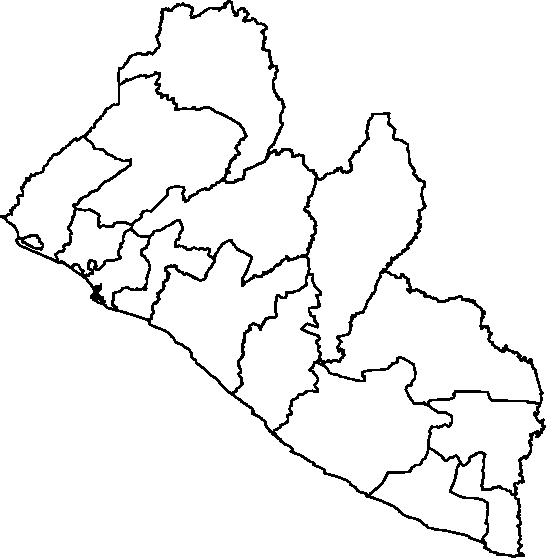
\includegraphics[keepaspectratio]{02_handling-spatial-data_files/figure-pdf/fig-liberia-admin-2.pdf}}

}

\subcaption{\label{fig-liberia-admin-2}Admin level 1}

\end{minipage}%

\caption{\label{fig-liberia-admin}Administrative boundaries for Liberia
retrieved using the \texttt{rgeoboundaries} package.}

\end{figure}%

\subsection{Example: Downloading population data}\label{sec-pop-data}

Population density is a key covariate in geostatistical models for
public health research. In this section, we demonstrate how to retrieve
high-resolution population data for Liberia from
\href{https://www.worldpop.org/}{WorldPop} using the
\texttt{wpgpDownloadR} package. This package provides easy access to the
WorldPop datasets, which offers gridded population estimates at various
spatial resolutions.

Before downloading the data, we will search for available datasets for
Liberia. The function \texttt{wpgpListCountryDatasets()} helps in
retrieving a list of all available datasets for a specified country.

\begin{Shaded}
\begin{Highlighting}[]
\FunctionTok{library}\NormalTok{(wpgpDownloadR)}

\CommentTok{\# Search for datasets available for Liberia }
\CommentTok{\# usign the ISO3 country code}
\NormalTok{lbr\_datasets }\OtherTok{\textless{}{-}} \FunctionTok{wpgpListCountryDatasets}\NormalTok{(}\AttributeTok{ISO3 =} \StringTok{"LBR"}\NormalTok{)}
\end{Highlighting}
\end{Shaded}

We can check the description column to see what datasets are available.
Let's download the population data for Liberia for the year 2014 at a
100m resolution. The \texttt{wpgpGetCountryDataset} function will then
download a raster dataset based on ISO3 code and covariate name.

\begin{Shaded}
\begin{Highlighting}[]
\NormalTok{lbr\_pop\_url }\OtherTok{\textless{}{-}} \FunctionTok{wpgpGetCountryDataset}\NormalTok{(}\AttributeTok{ISO3 =} \StringTok{"LBR"}\NormalTok{, }\AttributeTok{covariate =} \StringTok{"ppp\_2014"}\NormalTok{) }
\end{Highlighting}
\end{Shaded}

This will download a raster file locally in a temporary directory. The
path to the downloaded file is contained in the \texttt{lbr\_pop\_url}
variable and when we introduce the \texttt{terra} package in the next
sections we will show how to upoload the population raster into R. It is
also possible to specify the directory where we want the raster to be
downloaded using the \texttt{destDir} argument.

\subsection{Example: Dowloading data using Google Earth
Engine}\label{example-dowloading-data-using-google-earth-engine}

Google Earth Engine (GEE) is a powerful platform that hosts petabytes of
environmental and geospatial data, including climate, topography, and
land cover datasets. The \texttt{rgee} R package provides a convenient
interface to GEE from within R.

\begin{quote}
🔗 \textbf{Getting started with \texttt{rgee}}: To use \texttt{rgee},
you need a Google account and must complete a one-time setup process.
Follow the official guide here: \url{https://r-spatial.github.io/rgee/}.
For further tutorials and use cases, see:
\url{https://csaybar.github.io/rgee-examples/}.
\end{quote}

In this example, we retrieve elevation data for Liberia using the
\href{https://developers.google.com/earth-engine/datasets/catalog/CGIAR_SRTM90_V4}{SRTM
90m dataset}. The steps include initializing Earth Engine, access the
desired data product with the \texttt{ee\$Image("ASSET\_ID")} function
(the \texttt{ASSET\_ID} can be found on the dataset page under
\emph{Earth Engine Snippet}), converting the boundary of Liberia into a
format readable by GEE, clipping the global elevation raster to that
boundary, and downloading the result as a raster object in R. This
process demonstrates how \texttt{rgee} can be integrated into a
geostatistical workflow to enrich your data with high-quality
environmental covariates.

\begin{tcolorbox}[enhanced jigsaw, leftrule=.75mm, rightrule=.15mm, breakable, opacityback=0, coltitle=black, toprule=.15mm, toptitle=1mm, colbacktitle=quarto-callout-note-color!10!white, bottomrule=.15mm, opacitybacktitle=0.6, arc=.35mm, colback=white, title=\textcolor{quarto-callout-note-color}{\faInfo}\hspace{0.5em}{Note}, colframe=quarto-callout-note-color-frame, titlerule=0mm, bottomtitle=1mm, left=2mm]

This example assumes you have already completed \texttt{rgee} setup and
authenticated using \texttt{ee\_Initialize()}.

\end{tcolorbox}

\begin{Shaded}
\begin{Highlighting}[]
\CommentTok{\# Load required packages}
\FunctionTok{library}\NormalTok{(rgee)  }

\CommentTok{\# Initialize Earth Engine (first time will prompt browser login)}
\FunctionTok{ee\_Initialize}\NormalTok{(}\AttributeTok{quiet =}\NormalTok{ T)}

\CommentTok{\# Convert Liberia boundary to Earth Engine Geometry}
\NormalTok{liberia\_ee }\OtherTok{\textless{}{-}} \FunctionTok{sf\_as\_ee}\NormalTok{(liberia\_admin0)}

\CommentTok{\# Access the global SRTM elevation dataset from Earth Engine}
\NormalTok{elev }\OtherTok{\textless{}{-}}\NormalTok{ ee}\SpecialCharTok{$}\FunctionTok{Image}\NormalTok{(}\StringTok{"CGIAR/SRTM90\_V4"}\NormalTok{)}

\CommentTok{\# You can check general info about the data produc with ee\_print}
\FunctionTok{ee\_print}\NormalTok{(elev)}
\end{Highlighting}
\end{Shaded}

\begin{verbatim}
---------------------------------------------------------- Earth Engine Image --
Image Metadata:
 - Class                      : ee$Image
 - ID                         : CGIAR/SRTM90_V4
 - system:time_start          : 2000-02-11
 - system:time_end            : 2000-02-22
 - Number of Bands            : 1
 - Bands names                : elevation
 - Number of Properties       : 25
 - Number of Pixels*          : 62208576001
 - Approximate size*          : 17.53 GB
Band Metadata (img_band = elevation):
 - EPSG (SRID)                : WGS 84 (EPSG:4326)
 - proj4string                : +proj=longlat +datum=WGS84 +no_defs
 - Geotransform               : 0.000833333333333 0 -180 0 -0.000833333333333 60
 - Nominal scale (meters)     : 92.76624
 - Dimensions                 : 432001 144001
 - Number of Pixels           : 62208576001
 - Data type                  : INT
 - Approximate size           : 17.53 GB
 --------------------------------------------------------------------------------
 NOTE: (*) Properties calculated considering a constant geotransform and data type.
\end{verbatim}

\begin{Shaded}
\begin{Highlighting}[]
\CommentTok{\# Clip the elevation data to Liberia}
\NormalTok{elev\_liberia }\OtherTok{\textless{}{-}}\NormalTok{ elev}\SpecialCharTok{$}\FunctionTok{clip}\NormalTok{(liberia\_ee)}

\CommentTok{\# Download clipped elevation data as a raster using Google Drive}
\NormalTok{elev\_rast }\OtherTok{\textless{}{-}} \FunctionTok{ee\_as\_rast}\NormalTok{(}
  \AttributeTok{image =}\NormalTok{ elev\_liberia,}
  \AttributeTok{region =}\NormalTok{ liberia\_ee}\SpecialCharTok{$}\FunctionTok{geometry}\NormalTok{(),}
  \AttributeTok{via =} \StringTok{"drive"}\NormalTok{,}
  \AttributeTok{scale =} \DecValTok{1000}\NormalTok{, }\CommentTok{\# Aggregate to 1000 meters}
  \AttributeTok{quiet =}\NormalTok{ T}
\NormalTok{)}

\CommentTok{\# Replace 0s with NAs as these are usually elevation values }
\CommentTok{\# where no data exists due to clipping or ocean masking.}
\NormalTok{elev\_rast[elev\_rast }\SpecialCharTok{==} \DecValTok{0}\NormalTok{] }\OtherTok{\textless{}{-}} \ConstantTok{NA}

\CommentTok{\# Plot the result}
\NormalTok{terra}\SpecialCharTok{::}\FunctionTok{plot}\NormalTok{(elev\_rast, }\AttributeTok{main =} \StringTok{"Elevation in Liberia (m)"}\NormalTok{)}
\FunctionTok{plot}\NormalTok{(liberia\_admin0}\SpecialCharTok{$}\NormalTok{geometry, }\AttributeTok{add =}\NormalTok{ T)}
\end{Highlighting}
\end{Shaded}

\begin{figure}[H]

\centering{

\pandocbounded{
\includegraphics[keepaspectratio]{02_handling-spatial-data_files/figure-pdf/fig-rgee-elevation-1.pdf}}

}

\caption{\label{fig-rgee-elevation}Elevation (m) in Liberia retrieved
via Google Earth Engine (SRTM).}

\end{figure}%

\section{Importing and standardizing spatial
data}\label{importing-and-standardizing-spatial-data}

In geostatistical analysis, importing and standardizing spatial data is
a critical step to ensure that data from different sources align and can
be used effectively. Spatial data, whether it's vector data (points,
lines, polygons) or raster data (grids), can come in various formats and
may use different \textbf{Coordinate Reference Systems (CRS)}. To
perform accurate spatial analyses, it's essential to import data
correctly and ensure consistency in terms of projection and format. This
section will cover how to import vector and raster data into R, explain
the concept of CRS and sensure that different datasets align properly
for subsequent geostatistical analysis.

\subsection{Importing vector data}\label{importing-vector-data}

Vector data are typically stored in formats such as \textbf{shapefiles}
(\texttt{.shp}) or \textbf{geopackages} (\texttt{.gpkg}). The
\texttt{sf} (simple features) package in R is the most common tool for
handling vector data.

\begin{Shaded}
\begin{Highlighting}[]
\CommentTok{\# Load the sf package}
\FunctionTok{library}\NormalTok{(sf)}

\CommentTok{\# Import a shapefile (e.g., administrative boundaries)}
\NormalTok{admin }\OtherTok{\textless{}{-}} \FunctionTok{st\_read}\NormalTok{(}\StringTok{"path\_to\_your\_shapefile/Admin\_Boundaries.shp"}\NormalTok{)}

\CommentTok{\# Inspect the data}
\FunctionTok{print}\NormalTok{(admin)}
\FunctionTok{plot}\NormalTok{(admin)  }\CommentTok{\# Basic plot of the shapefile}
\end{Highlighting}
\end{Shaded}

The \texttt{st\_read()} function reads various spatial data formats,
automatically recognizing file types.

\subsection{Importing raster data}\label{importing-raster-data}

Raster data consists of a grid of cells, where each cell holds a value
representing a spatial attribute such as elevation or temperature. The
\texttt{terra} package in R is designed to work with raster data and has
superseded the older \texttt{raster} package due to better performance
and greater functionality. Let's see now how to import a GeoTIFF file
using \texttt{terra}. We can upload the population raster for Liberia
that we have downloaded in Section~\ref{sec-pop-data}.

\begin{Shaded}
\begin{Highlighting}[]
\CommentTok{\# Import a raster file }
\NormalTok{lbr\_pop\_100 }\OtherTok{\textless{}{-}} \FunctionTok{rast}\NormalTok{(lbr\_pop\_url)}
\end{Highlighting}
\end{Shaded}

\begin{Shaded}
\begin{Highlighting}[]
\CommentTok{\# Load the terra package}
\FunctionTok{library}\NormalTok{(terra)}

\CommentTok{\# Inspect the raster data}
\FunctionTok{print}\NormalTok{(lbr\_pop\_100)}
\end{Highlighting}
\end{Shaded}

\begin{verbatim}
class       : SpatRaster 
size        : 5040, 4945, 1  (nrow, ncol, nlyr)
resolution  : 0.0008333333, 0.0008333333  (x, y)
extent      : -11.48625, -7.365417, 4.352084, 8.552084  (xmin, xmax, ymin, ymax)
coord. ref. : lon/lat WGS 84 (EPSG:4326) 
source      : lbr_pop_100.tif 
name        : lbr_ppp_2014 
min value   :  0.006426936 
max value   : 92.716873169 
\end{verbatim}

\begin{Shaded}
\begin{Highlighting}[]
\CommentTok{\# Basic plot of the raster (log{-}scale)}
\FunctionTok{plot}\NormalTok{(}\FunctionTok{log}\NormalTok{(lbr\_pop\_100), }\AttributeTok{main =} \StringTok{"Population per 100m (log{-}scale)"}\NormalTok{)}
\FunctionTok{plot}\NormalTok{(liberia\_admin0}\SpecialCharTok{$}\NormalTok{geometry, }\AttributeTok{add =}\NormalTok{ T)}
\end{Highlighting}
\end{Shaded}

\begin{figure}[H]

\centering{

\pandocbounded{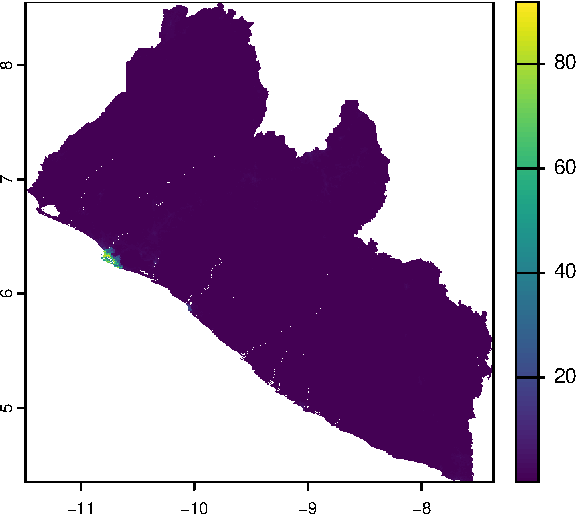
\includegraphics[keepaspectratio]{02_handling-spatial-data_files/figure-pdf/fig-lbr-pop-1.pdf}}

}

\caption{\label{fig-lbr-pop}Liberia population count for 2014 at 100m
resolution (log-scale).}

\end{figure}%

The output of \texttt{print()} provides a detailed summary of the
raster's properties. The \texttt{rast()} function reads raster files in
formats like GeoTIFF, ASCII grid, or other common raster formats and
then we used \texttt{plot()} as a quick way to visualize raster data.

\subsection{Understanding coordinate reference systems
(CRS)}\label{understanding-coordinate-reference-systems-crs}

When working with spatial data, especially from different sources, one
of the most critical tasks is ensuring that all datasets share the same
\textbf{Coordinate Reference System (CRS)}. A CRS defines how the
two-dimensional map data corresponds to locations on the
three-dimensional Earth. If different layers (e.g., raster and vector
data) have different CRSs, they may not align correctly when plotted or
analyzed together, leading to inaccurate analyses or visualizations.

CRSs can either be:

\begin{itemize}
\item
  \textbf{Geographic}: These use latitude and longitude coordinates to
  represent locations on the Earth's surface. The most common example is
  \textbf{WGS84} (EPSG:4326), the default CRS used by GPS and global
  datasets.
\item
  \textbf{Projected}: These convert the Earth's curved surface to a flat
  map and preserve certain properties like area, distance, or direction.
  Examples include \textbf{Universal Transverse Mercator (UTM)} or
  \textbf{Albers Equal Area} projections.
\end{itemize}

In many cases, using a projected rather than a geographic CRS is
preferred, especially when any summary statistic or parameter is
distance-related. In a geographic CRS, distances between two points are
calculated using angular coordinates (degrees), which do not translate
easily into linear units like meters or kilometers. This makes
interpreting distances challenging, as the length of a degree of
latitude differs from the length of a degree of longitude. In contrast,
a projected CRS uses a linear coordinate system (usually meters),
ensuring that distances are accurately represented on a flat surface.
This is important when computing spatial variograms, covariance
functions, or some parameters in geostatistical models, where distance
between sampling locations is a key factor. In this context, we assume
that the default distance metric is Euclidean distance. However, an
important exception to our recommendation arises when analyzing data
across large, global-scale regions. In such cases, it is more
appropriate to use a geographic CRS along with spherical distances, as
these better reflect the curved nature of the Earth's surface.

\subsection{EPSG codes}\label{epsg-codes}

An \textbf{EPSG code} is a unique identifier that defines a CRS. These
codes, managed by the \textbf{European Petroleum Survey Group (EPSG)},
are widely used in geographic information systems (GIS) to simplify the
use of specific projections, ensuring that spatial data is correctly
aligned and interpreted. Each EPSG code corresponds to a unique CRS or
map projection, making it easier to standardize and manage spatial data
from different sources.

Some key and often used EPSG codes are:

\begin{itemize}
\item
  \textbf{EPSG:4326}: This code represents \textbf{WGS84}, the most
  commonly used geographic CRS, which uses latitude and longitude to
  describe locations on the Earth's surface. It is the default CRS for
  global datasets and GPS systems.
\item
  \textbf{EPSG:326XX}: These codes represent the \textbf{UTM (Universal
  Transverse Mercator)} projection, which divides the world into zones.
  Each zone is optimized to preserve local distances and areas. For
  example (e.g.~EPSG:32629: UTM Zone 29N, covering parts of Western
  Africa, including Liberia)
\item
  \textbf{EPSG:3857}: This code is for the \textbf{Web Mercator
  projection}, which is widely used for web mapping services, including
  \textbf{Google Maps}, \textbf{OpenStreetMap}, and \textbf{Bing Maps}.
  This projected CRS uses meters as the unit of distance and is
  optimized for visualizing maps on a 2D plane, though it distorts area
  and distance, especially at high latitudes. It is well-suited for
  interactive online mapping but not ideal for precise distance-based
  geostatistical analyses.
\end{itemize}

For a more in-depth discussion on how to choose an appropriate CRS, we
recommend referring to the excellent treatment in
\href{https://r.geocompx.org}{\emph{Geocomputation with R}} (Lovelace,
Nowosad, and Muenchow 2020), especially
\href{https://r.geocompx.org/reproj-geo-data\#which-crs}{Section 7.6:
Which CRS?}.

\subsection{\texorpdfstring{Convert a data frame to an \texttt{sf}
object}{Convert a data frame to an sf object}}\label{convert-a-data-frame-to-an-sf-object}

In geospatial analysis, data is often provided in tabular formats like
CSV files that contain spatial coordinates (e.g., latitude and
longitude). To use these data effectively in R, it is necessary to
convert the data frame into an \texttt{sf} object, which is the standard
format for working with spatial data in R. Here we show how to achieve
this, we can use the Liberia data available in the \texttt{RiskMap}
package as it is a data frame.

\begin{Shaded}
\begin{Highlighting}[]
\CommentTok{\# Load the RiskMap package}
\FunctionTok{library}\NormalTok{(RiskMap)}

\CommentTok{\# Load the Liberia data set}
\FunctionTok{data}\NormalTok{(}\StringTok{"liberia"}\NormalTok{)}

\CommentTok{\# Convert the data frame to an sf object}
\NormalTok{liberia\_sf }\OtherTok{\textless{}{-}} \FunctionTok{st\_as\_sf}\NormalTok{(liberia, }
                       \AttributeTok{coords =} \FunctionTok{c}\NormalTok{(}\StringTok{"long"}\NormalTok{, }\StringTok{"lat"}\NormalTok{), }
                       \AttributeTok{crs =} \DecValTok{4326}\NormalTok{)}

\CommentTok{\# Inspect the new sf object}
\NormalTok{liberia\_sf}
\end{Highlighting}
\end{Shaded}

\begin{verbatim}
Simple feature collection with 90 features and 4 fields
Geometry type: POINT
Dimension:     XY
Bounding box:  xmin: -11.40335 ymin: 4.42552 xmax: -7.4928 ymax: 8.46911
Geodetic CRS:  WGS 84
First 10 features:
   ntest npos elevation log_elevation                   geometry
1     50   14  17.82621      2.880670    POINT (-10.4671 6.2878)
2     46   10 104.85070      4.652537   POINT (-10.45111 6.5725)
3     43   11 119.09543      4.779925  POINT (-10.02615 6.56667)
4     50   10 144.10921      4.970571  POINT (-10.28775 6.73333)
5     48    9  19.03508      2.946283 POINT (-10.03595 6.016667)
6     50   13  16.99954      2.833186   POINT (-10.335 6.266666)
7     43    9 137.75360      4.925467   POINT (-9.63333 6.13541)
8     50   11 101.75000      4.622519   POINT (-10.06875 6.2375)
9     47   11 147.12867      4.991308    POINT (-9.73333 6.3869)
10    43    0  26.61054      3.281308     POINT (-9.7856 5.7354)
\end{verbatim}

\begin{Shaded}
\begin{Highlighting}[]
\FunctionTok{par}\NormalTok{(}\AttributeTok{mar =} \FunctionTok{c}\NormalTok{(}\DecValTok{0}\NormalTok{, }\DecValTok{0}\NormalTok{, }\DecValTok{0}\NormalTok{, }\DecValTok{0}\NormalTok{))  }\CommentTok{\#| hide\_line}
\FunctionTok{plot}\NormalTok{(liberia\_sf)}
\end{Highlighting}
\end{Shaded}

\pandocbounded{
\includegraphics[keepaspectratio]{02_handling-spatial-data_files/figure-pdf/st-as-sf-1.pdf}}

The \texttt{st\_as\_sf()} function converts the data frame into an
\texttt{sf} object. The \texttt{coords} argument specifies which columns
contain the spatial coordinates and the \texttt{crs} argument assigns
the CRS that in this case we know being WGS84 (EPSG:4326). The
\texttt{sf} object can now be used for operations such as spatial joins,
distance calculations, and mapping with other spatial layers. Note that
the columns containing the spatial coordinates have been replaced by a
\texttt{geometry} column, which now stores this information. If you
would like to retain the original coordinate columns in the output, you
can set the \texttt{remove} argument to \texttt{FALSE} when converting
the data frame to an \texttt{sf} object.

\subsection{Working with CRSs in R}\label{working-with-crss-in-r}

When working with data from multiple sources, such as environmental
layers, population data, or administrative boundaries, ensuring that all
datasets share the same CRS is essential for accurate spatial analysis.
This section covers the core tasks involved in managing CRSs in R:
checking the CRS of spatial data to ensure datasets are compatible and
reprojecting spatial data into a common CRS when necessary.

\subsubsection{Checking the CRS of Spatial
Data}\label{checking-the-crs-of-spatial-data}

Before performing any spatial operation, it's crucial to check the CRS
of your spatial datasets. Knowing whether your data uses geographic
coordinates (e.g., WGS84) or a projected coordinate system (e.g., UTM)
helps ensure that they are aligned and ready for analysis. Both
\texttt{sf} and \texttt{terra} provide functions to retrieve and inspect
the CRS, ensuring datasets are spatially aligned before analysis. The
\texttt{st\_crs()} function retrieves the CRS information for vector
data.

\begin{Shaded}
\begin{Highlighting}[]
\CommentTok{\# Check the CRS of the vector data}
\FunctionTok{st\_crs}\NormalTok{(liberia\_sf)}
\end{Highlighting}
\end{Shaded}

\begin{verbatim}
Coordinate Reference System:
  User input: EPSG:4326 
  wkt:
GEOGCRS["WGS 84",
    ENSEMBLE["World Geodetic System 1984 ensemble",
        MEMBER["World Geodetic System 1984 (Transit)"],
        MEMBER["World Geodetic System 1984 (G730)"],
        MEMBER["World Geodetic System 1984 (G873)"],
        MEMBER["World Geodetic System 1984 (G1150)"],
        MEMBER["World Geodetic System 1984 (G1674)"],
        MEMBER["World Geodetic System 1984 (G1762)"],
        MEMBER["World Geodetic System 1984 (G2139)"],
        ELLIPSOID["WGS 84",6378137,298.257223563,
            LENGTHUNIT["metre",1]],
        ENSEMBLEACCURACY[2.0]],
    PRIMEM["Greenwich",0,
        ANGLEUNIT["degree",0.0174532925199433]],
    CS[ellipsoidal,2],
        AXIS["geodetic latitude (Lat)",north,
            ORDER[1],
            ANGLEUNIT["degree",0.0174532925199433]],
        AXIS["geodetic longitude (Lon)",east,
            ORDER[2],
            ANGLEUNIT["degree",0.0174532925199433]],
    USAGE[
        SCOPE["Horizontal component of 3D system."],
        AREA["World."],
        BBOX[-90,-180,90,180]],
    ID["EPSG",4326]]
\end{verbatim}

The same can be achieved for raster data with the \texttt{crs()}
function from the \texttt{terra} package.

\begin{Shaded}
\begin{Highlighting}[]
\CommentTok{\# Check the CRS of the raster data}
\FunctionTok{crs}\NormalTok{(lbr\_pop\_100, }\AttributeTok{proj =} \ConstantTok{TRUE}\NormalTok{, }\AttributeTok{describe =} \ConstantTok{TRUE}\NormalTok{)}
\end{Highlighting}
\end{Shaded}

\begin{verbatim}
    name authority code  area             extent
1 WGS 84      EPSG 4326 World -180, 180, -90, 90
                                 proj
1 +proj=longlat +datum=WGS84 +no_defs
\end{verbatim}

\subsubsection{Reprojecting spatial data to a common
CRS}\label{reprojecting-spatial-data-to-a-common-crs}

If your datasets have different CRSs or if you want to change CRS
(e.g.~from geographical to projected) you will need to reproject one or
more datasets so they can be spatially aligned. This ensures that they
can be overlaid and analyzed together. For vector data,
\texttt{st\_transform()} reprojects the data into a specified CRS. This
example transforms the liberia point data from WGS84 into UTM. To know
what's the correct UTM zone and hence EPSG code for Liberia we can use
the \texttt{propose\_utm} function from the \texttt{RiskMap} package.

\begin{Shaded}
\begin{Highlighting}[]
\CommentTok{\# Obtain EPSG code for UTM for Liberia}
\FunctionTok{propose\_utm}\NormalTok{(liberia\_sf)}
\end{Highlighting}
\end{Shaded}

\begin{verbatim}
[1] 32629
\end{verbatim}

\begin{Shaded}
\begin{Highlighting}[]
\CommentTok{\# Reproject the vector data }
\NormalTok{liberia\_sf\_utm }\OtherTok{\textless{}{-}} \FunctionTok{st\_transform}\NormalTok{(liberia\_sf, }\AttributeTok{crs =} \FunctionTok{propose\_utm}\NormalTok{(liberia\_sf))}
\end{Highlighting}
\end{Shaded}

Reprojecting raster data is more complex than reprojecting vector data
due to the continuous nature of raster grids. The process involves
recalculating cell values to fit a new grid based on the new CRS, which
can lead to challenges like resampling, distortion, and data loss. When
reprojecting a raster, the grid must adjust to the new CRS, often
requiring resampling of cell values. The method you choose depends on
the data type: \textbf{nearest neighbor} is best for categorical data
like land use while \textbf{bilinear or cubic interpolation} is good for
continuous data like temperature, where smooth transitions are needed.

The function \texttt{project()} from the \texttt{terra} package can be
used to project a raster.

\begin{Shaded}
\begin{Highlighting}[]
\NormalTok{lbr\_pop\_100\_utm }\OtherTok{\textless{}{-}} \FunctionTok{project}\NormalTok{(lbr\_pop\_100, }
                           \FunctionTok{crs}\NormalTok{(liberia\_sf\_utm),}
                           \AttributeTok{method =} \StringTok{"bilinear"}\NormalTok{)}
\end{Highlighting}
\end{Shaded}

Reprojecting a raster may alter its resolution. For example,
reprojecting from geographic (degrees) to projected (meters) CRS can
result in a mismatch between the original and new cell sizes. Moreover,
distortion can occur when converting between projections, especially at
high latitudes. Some cells may be stretched or compressed, leading to
potential loss of information or edge artifacts. These distortions arise
because the Earth is not flat, and projecting the curved surface of the
Earth onto a flat plane (or vice versa) leads to trade-offs. For
example, the Mercator projection preserves angles and shapes but
distorts area, particularly near the poles.

For these reasons, it's often better to reproject vectors rather than
rasters when both data types are used together and avoid as much as
possible to change the CRS of rasters. One way to achieve this is to
work with WGS84 when performing all spatial operations like extraction
of covariates from rasters and then transform only the point data to a
projected CRS before fitting the model.

\section{Extracting covariate data}\label{extracting-covariate-data}

In geostatistical models, the inclusion of relevant covariates
(environmental, demographic, or climatic) can potentially enhance
predictive accuracy. Covariate data often come from raster or polygon
sources, and extracting these values for point locations is essential to
link spatial context to point-referenced data. These covariates could
include variables like temperature, elevation, land cover, or population
density, which influence the spatial distribution of diseases. In this
section, we will cover how to extract covariates at point locations from
both polygon and raster layers.

\subsubsection{Extracting covariates from polygon
layers}\label{extracting-covariates-from-polygon-layers}

Polygon layers represent discrete spatial features such as
administrative boundaries, land cover categories, or protected areas.
These layers typically include associated attributes (e.g.~region names,
population totals, land type), which can serve as covariates in
geostatistical models. A common task in spatial data analysis is to
assign attributes from a polygon layer to a set of point-referenced
data, for example, determining the administrative region or land use
category that each survey location falls within. This is done using a
\textbf{spatial join}, which overlays the point and polygon layers and
attaches the attributes of the enclosing polygon to each point. Below is
an example where we assign administrative region names (admin1) to a set
of point locations in Liberia:

\begin{Shaded}
\begin{Highlighting}[]
\CommentTok{\# Perform a spatial join to transfer polygon attributes to the points}
\NormalTok{points\_with\_admin }\OtherTok{\textless{}{-}} \FunctionTok{st\_join}\NormalTok{(liberia\_sf, liberia\_admin1[}\StringTok{"shapeName"}\NormalTok{])}

\CommentTok{\# View the results, points now include covariates from the polygon layer}
\FunctionTok{head}\NormalTok{(points\_with\_admin)}
\end{Highlighting}
\end{Shaded}

\begin{verbatim}
Simple feature collection with 6 features and 5 fields
Geometry type: POINT
Dimension:     XY
Bounding box:  xmin: -10.4671 ymin: 6.016667 xmax: -10.02615 ymax: 6.73333
Geodetic CRS:  WGS 84
  ntest npos elevation log_elevation   shapeName                   geometry
1    50   14  17.82621      2.880670     Margibi    POINT (-10.4671 6.2878)
2    46   10 104.85070      4.652537 Montserrado   POINT (-10.45111 6.5725)
3    43   11 119.09543      4.779925     Margibi  POINT (-10.02615 6.56667)
4    50   10 144.10921      4.970571     Margibi  POINT (-10.28775 6.73333)
5    48    9  19.03508      2.946283 Grand Bassa POINT (-10.03595 6.016667)
6    50   13  16.99954      2.833186 Grand Bassa   POINT (-10.335 6.266666)
\end{verbatim}

This spatial join enriches each point with the corresponding polygon
attribute, in this case, the admin1 name (shapeName). These attributes
can then be used as categorical covariates in geostatistical models to
account for regional variation in disease risk or programmatic coverage.

\subsection{Extracting covariates from raster
layers}\label{extracting-covariates-from-raster-layers}

Raster data provides continuous spatial information, such as elevation,
climate data, or population density. Covariate values from raster layers
can be extracted for specific points using the
\textbf{\texttt{extract()}} function from the \texttt{terra} package.
Each point will receive the value of the raster cell it overlaps.

\begin{Shaded}
\begin{Highlighting}[]
\CommentTok{\# Extract raster values at the point locations}
\NormalTok{covariate\_values }\OtherTok{\textless{}{-}} \FunctionTok{extract}\NormalTok{(lbr\_pop\_100, liberia\_sf)}

\CommentTok{\# Combine the extracted values with the point data}
\NormalTok{liberia\_sf}\SpecialCharTok{$}\NormalTok{pop\_total }\OtherTok{\textless{}{-}}\NormalTok{ covariate\_values[, }\DecValTok{2}\NormalTok{]}

\CommentTok{\# View the updated dataset}
\FunctionTok{head}\NormalTok{(liberia\_sf)}
\end{Highlighting}
\end{Shaded}

\begin{verbatim}
Simple feature collection with 6 features and 5 fields
Geometry type: POINT
Dimension:     XY
Bounding box:  xmin: -10.4671 ymin: 6.016667 xmax: -10.02615 ymax: 6.73333
Geodetic CRS:  WGS 84
  ntest npos elevation log_elevation                   geometry pop_total
1    50   14  17.82621      2.880670    POINT (-10.4671 6.2878) 0.2914019
2    46   10 104.85070      4.652537   POINT (-10.45111 6.5725) 0.6087928
3    43   11 119.09543      4.779925  POINT (-10.02615 6.56667) 0.2044306
4    50   10 144.10921      4.970571  POINT (-10.28775 6.73333) 0.5078438
5    48    9  19.03508      2.946283 POINT (-10.03595 6.016667) 0.1767686
6    50   13  16.99954      2.833186   POINT (-10.335 6.266666) 1.6693381
\end{verbatim}

In this example, the \texttt{extract()} function assigns the raster
value from the population density layer to each point in the dataset.
This allows the point data to include population density as a covariate
in the analysis.

Instead of extracting values for exact point locations, it can sometimes
be useful to aggregate covariate values within a defined area around
each point. This is often done by creating a buffer around each point
and calculating summary statistics (e.g., mean, sum) of the raster
values within that buffer. For instance, you might want to calculate the
average population density or temperature within a 5 km radius around
each point to smooth out fine-scale variation.

\begin{Shaded}
\begin{Highlighting}[]
\CommentTok{\# Create buffers around each point (e.g., 5 km radius)}
\NormalTok{buffered\_points }\OtherTok{\textless{}{-}} \FunctionTok{st\_buffer}\NormalTok{(liberia\_sf\_utm, }\AttributeTok{dist =} \DecValTok{5000}\NormalTok{)  }

\CommentTok{\# Plot the buffers for visualization}
\FunctionTok{par}\NormalTok{(}\AttributeTok{mar =} \FunctionTok{c}\NormalTok{(}\DecValTok{0}\NormalTok{, }\DecValTok{0}\NormalTok{, }\DecValTok{0}\NormalTok{, }\DecValTok{0}\NormalTok{))  }\CommentTok{\#| hide\_line}
\FunctionTok{plot}\NormalTok{(}\FunctionTok{st\_geometry}\NormalTok{(buffered\_points), }\AttributeTok{border =} \StringTok{"black"}\NormalTok{)}
\FunctionTok{plot}\NormalTok{(}\FunctionTok{st\_geometry}\NormalTok{(liberia\_sf\_utm), }\AttributeTok{add =}\NormalTok{ T, }\AttributeTok{pch =} \DecValTok{19}\NormalTok{, }\AttributeTok{col =} \StringTok{"red"}\NormalTok{, }\AttributeTok{cex =}\NormalTok{ .}\DecValTok{2}\NormalTok{)}
\end{Highlighting}
\end{Shaded}

\begin{figure}[H]

\centering{

\pandocbounded{
\includegraphics[keepaspectratio]{02_handling-spatial-data_files/figure-pdf/fig-buffer-extract-1.pdf}}

}

\caption{\label{fig-buffer-extract}Survey locations (red dots)
surrounded by a 5 km buffer (dark circles).}

\end{figure}%

\begin{Shaded}
\begin{Highlighting}[]
\CommentTok{\# Extract raster values within the buffer areas and calculate the }
\CommentTok{\# mean or sum. Note that since we used the utm data to work on the}
\CommentTok{\# meter scale we need to convert them back to WGS84}
\NormalTok{mean\_pop\_density }\OtherTok{\textless{}{-}} \FunctionTok{extract}\NormalTok{(lbr\_pop\_100, }
                            \FunctionTok{st\_transform}\NormalTok{(buffered\_points, }\AttributeTok{crs =} \DecValTok{4326}\NormalTok{),}
                            \AttributeTok{fun =}\NormalTok{ mean, }\AttributeTok{na.rm =} \ConstantTok{TRUE}\NormalTok{)}

\CommentTok{\# Add the averaged values to the points dataset}
\NormalTok{liberia\_sf}\SpecialCharTok{$}\NormalTok{pop\_mean5km }\OtherTok{\textless{}{-}}\NormalTok{ mean\_pop\_density[,}\DecValTok{2}\NormalTok{]}

\CommentTok{\# View the updated dataset}
\FunctionTok{head}\NormalTok{(liberia\_sf)}
\end{Highlighting}
\end{Shaded}

\begin{verbatim}
Simple feature collection with 6 features and 6 fields
Geometry type: POINT
Dimension:     XY
Bounding box:  xmin: -10.4671 ymin: 6.016667 xmax: -10.02615 ymax: 6.73333
Geodetic CRS:  WGS 84
  ntest npos elevation log_elevation                   geometry pop_total
1    50   14  17.82621      2.880670    POINT (-10.4671 6.2878) 0.2914019
2    46   10 104.85070      4.652537   POINT (-10.45111 6.5725) 0.6087928
3    43   11 119.09543      4.779925  POINT (-10.02615 6.56667) 0.2044306
4    50   10 144.10921      4.970571  POINT (-10.28775 6.73333) 0.5078438
5    48    9  19.03508      2.946283 POINT (-10.03595 6.016667) 0.1767686
6    50   13  16.99954      2.833186   POINT (-10.335 6.266666) 1.6693381
  pop_mean5km
1   0.6015397
2   0.5565529
3   0.2488039
4   0.5604327
5   0.2877019
6   2.0974484
\end{verbatim}

You can modify the \texttt{fun} argument to calculate other summary
statistics, such as the sum, min or max of the raster values within the
buffer. This approach is particularly useful when the phenomenon being
modeled (e.g., disease transmission) is influenced by broader spatial
factors around the observation point, rather than just the value at the
exact point location.

\section{Creating a predictive grid}\label{creating-a-predictive-grid}

A predictive grid is a regularly spaced set of points or cells that
spans the study region. This grid serves as the basis for predictions
made by your model. The density of the grid (i.e., the distance between
grid points) affects both the resolution of the prediction and the
computational cost. For point-based predictions, we can generate a grid
of points over a polygon (e.g., administrative boundary) using the
\texttt{sf} package and the \texttt{st\_make\_grid} function.

\begin{Shaded}
\begin{Highlighting}[]
\CommentTok{\# First we convert the Liberia boundaries to the UTM CRS}
\CommentTok{\# because we want our grid in meters}
\NormalTok{liberia\_admin0\_utm }\OtherTok{\textless{}{-}}\NormalTok{ liberia\_admin0 }\SpecialCharTok{|\textgreater{}} 
  \FunctionTok{st\_transform}\NormalTok{(}\AttributeTok{crs =} \FunctionTok{propose\_utm}\NormalTok{(liberia\_sf))}

\CommentTok{\# Generate prediction grid at 5km resolution}
\NormalTok{pred\_locations }\OtherTok{\textless{}{-}} \FunctionTok{st\_make\_grid}\NormalTok{(liberia\_admin0\_utm, }
                               \AttributeTok{cellsize =} \DecValTok{5000}\NormalTok{, }
                               \AttributeTok{what =} \StringTok{"centers"}\NormalTok{)}

\CommentTok{\# Exclude locations that fall outside the study area}
\NormalTok{pred\_locations }\OtherTok{\textless{}{-}} \FunctionTok{st\_intersection}\NormalTok{(pred\_locations, liberia\_admin0\_utm)}

\CommentTok{\# Visualize the result}
\FunctionTok{par}\NormalTok{(}\AttributeTok{mar =} \FunctionTok{c}\NormalTok{(}\DecValTok{0}\NormalTok{, }\DecValTok{0}\NormalTok{, }\DecValTok{0}\NormalTok{, }\DecValTok{0}\NormalTok{))  }\CommentTok{\#| hide\_line}
\FunctionTok{plot}\NormalTok{(liberia\_admin0\_utm}\SpecialCharTok{$}\NormalTok{geometry, }\AttributeTok{col =} \StringTok{"white"}\NormalTok{)}
\FunctionTok{plot}\NormalTok{(pred\_locations, }\AttributeTok{cex =}\NormalTok{ .}\DecValTok{01}\NormalTok{, }\AttributeTok{col =} \StringTok{"red"}\NormalTok{, }\AttributeTok{pch =} \DecValTok{19}\NormalTok{, }\AttributeTok{add =}\NormalTok{ T)}
\end{Highlighting}
\end{Shaded}

\begin{figure}[H]

\centering{

\pandocbounded{
\includegraphics[keepaspectratio]{02_handling-spatial-data_files/figure-pdf/fig-pred-grid-1.pdf}}

}

\caption{\label{fig-pred-grid}Prediction grid (5 km spacing) created
within the boundaries of Liberia. Points are spaced regularly in UTM
coordinates and filtered to remain within the national boundary.}

\end{figure}%

\section{Visualizing spatial data}\label{visualizing-spatial-data}

Visualization is a key part of spatial data analysis, as it allows you
to explore and communicate spatial patterns and relationships
effectively. R provides a lot of functionalities to visualize spatial
data and create very beautiful maps. Until now we have used basic
plotting functions. Here we introduce the \texttt{ggplot2} package that
allows to combine different types of geographic data in a map. The
\texttt{ggplot2} package in R provides a flexible and powerful framework
for creating both simple and complex visualizations, including maps of
point data, polygons, and rasters. With the help of extensions like
\texttt{geom\_sf()} and \texttt{geom\_raster()}, \texttt{ggplot2} makes
it easy to visualize spatial data, whether you're working with point
locations, polygons, or continuous raster data.

\subsection{Visualizing point data}\label{visualizing-point-data}

Point data often represents the locations of observations (e.g., disease
cases, sampling sites). \texttt{ggplot2} allows you to plot these points
and optionally color them by a covariate (e.g., disease prevalence or
population density). Here is an example that uses the Liberia data.

\begin{Shaded}
\begin{Highlighting}[]
\CommentTok{\# Load necessary libraries}
\FunctionTok{library}\NormalTok{(ggplot2)}

\CommentTok{\# Create a new variable with prevalence in the dataset}
\NormalTok{liberia\_sf}\SpecialCharTok{$}\NormalTok{prevalence }\OtherTok{\textless{}{-}}\NormalTok{ liberia}\SpecialCharTok{$}\NormalTok{npos }\SpecialCharTok{/}\NormalTok{ liberia}\SpecialCharTok{$}\NormalTok{ntest}

\CommentTok{\# Plot only the locations}
\FunctionTok{ggplot}\NormalTok{(}\AttributeTok{data =}\NormalTok{ liberia\_sf) }\SpecialCharTok{+}
  \FunctionTok{geom\_sf}\NormalTok{(}\AttributeTok{col =} \StringTok{"black"}\NormalTok{) }\SpecialCharTok{+}  
  \FunctionTok{theme\_minimal}\NormalTok{() }\SpecialCharTok{+}
  \FunctionTok{labs}\NormalTok{(}\AttributeTok{title =} \StringTok{"Survey locations"}\NormalTok{)}

\CommentTok{\# Color the points according to prevalence}
\FunctionTok{ggplot}\NormalTok{(}\AttributeTok{data =}\NormalTok{ liberia\_sf) }\SpecialCharTok{+}
  \FunctionTok{geom\_sf}\NormalTok{(}\FunctionTok{aes}\NormalTok{(}\AttributeTok{color =}\NormalTok{ prevalence)) }\SpecialCharTok{+}  
  \FunctionTok{scale\_color\_viridis\_c}\NormalTok{(}\AttributeTok{labels =}\NormalTok{ scales}\SpecialCharTok{::}\FunctionTok{label\_percent}\NormalTok{()) }\SpecialCharTok{+}  
  \FunctionTok{theme\_minimal}\NormalTok{() }\SpecialCharTok{+}
  \FunctionTok{labs}\NormalTok{(}\AttributeTok{title =} \StringTok{"Onchocerciasis in Liberia"}\NormalTok{,}
       \AttributeTok{color =} \StringTok{"Prevalence (\%)"}\NormalTok{)}
\end{Highlighting}
\end{Shaded}

\begin{figure}

\begin{minipage}{0.50\linewidth}

\centering{

\pandocbounded{
\includegraphics[keepaspectratio]{02_handling-spatial-data_files/figure-pdf/fig-ggplot-points-1.pdf}}

}

\subcaption{\label{fig-ggplot-points-1}Survey locations.}

\end{minipage}%
%
\begin{minipage}{0.50\linewidth}

\centering{

\pandocbounded{
\includegraphics[keepaspectratio]{02_handling-spatial-data_files/figure-pdf/fig-ggplot-points-2.pdf}}

}

\subcaption{\label{fig-ggplot-points-2}Survey locations colored by
prevalence.}

\end{minipage}%

\caption{\label{fig-ggplot-points}Using \texttt{geom\_sf()} to plot
point data.}

\end{figure}%

Here \texttt{geom\_sf()} is used to plot the spatial points.
\texttt{aes(color\ =\ prevalence)} specifies that the points should be
colored based on the \texttt{prevalence} covariate, providing a visual
representation of spatial variation in disease risk. The
\texttt{scale\_color\_viridis\_c()} function applies the Viridis color
scale, which is well-suited for continuous data and is friendly for
those with color blindness. The
\texttt{labels\ =\ scales::label\_percent()} argument ensures that the
color scale's labels are displayed as percentages (e.g., 5, 10\%) rather
than raw decimal values. To make the plot visually clean and minimal,
\texttt{theme\_minimal()} is applied, stripping away unnecessary
background elements and keeping the focus on the data. Finally, the
\texttt{labs()} defines the plot title and the color legend label.

\subsection{Visualizing polygon data}\label{visualizing-polygon-data}

Polygon data typically represents administrative boundaries, land use,
or other regional divisions. We can still use \texttt{geom\_sf()} to
create maps of polygons, optionally filling them by a covariate.

\begin{Shaded}
\begin{Highlighting}[]
\CommentTok{\# Plot Liberia admin 1 level boundaries }
\FunctionTok{ggplot}\NormalTok{(}\AttributeTok{data =}\NormalTok{ liberia\_admin1) }\SpecialCharTok{+}
  \FunctionTok{geom\_sf}\NormalTok{() }\SpecialCharTok{+} 
  \FunctionTok{theme\_minimal}\NormalTok{() }\SpecialCharTok{+}
  \FunctionTok{labs}\NormalTok{()}

\CommentTok{\# We compute the area of each polygon}
\NormalTok{liberia\_admin1}\SpecialCharTok{$}\NormalTok{area }\OtherTok{\textless{}{-}} \FunctionTok{as.numeric}\NormalTok{(}\FunctionTok{st\_area}\NormalTok{(liberia\_admin1) }\SpecialCharTok{/} \DecValTok{1000} \SpecialCharTok{\^{}} \DecValTok{2}\NormalTok{)}

\CommentTok{\# Color the polygons according tis new variable}
\FunctionTok{ggplot}\NormalTok{(}\AttributeTok{data =}\NormalTok{ liberia\_admin1) }\SpecialCharTok{+}
  \FunctionTok{geom\_sf}\NormalTok{(}\FunctionTok{aes}\NormalTok{(}\AttributeTok{fill =}\NormalTok{ area), }\AttributeTok{color =} \StringTok{"black"}\NormalTok{) }\SpecialCharTok{+} 
  \FunctionTok{scale\_fill\_distiller}\NormalTok{(}\AttributeTok{direction =} \SpecialCharTok{{-}}\DecValTok{1}\NormalTok{) }\SpecialCharTok{+}
  \FunctionTok{theme\_minimal}\NormalTok{() }\SpecialCharTok{+}
  \FunctionTok{labs}\NormalTok{(}\AttributeTok{fill =} \StringTok{"Area km\^{}2"}\NormalTok{)}
\end{Highlighting}
\end{Shaded}

\begin{figure}

\begin{minipage}{0.50\linewidth}

\centering{

\pandocbounded{
\includegraphics[keepaspectratio]{02_handling-spatial-data_files/figure-pdf/fig-ggplot-polygons-1.pdf}}

}

\subcaption{\label{fig-ggplot-polygons-1}Admin 1 units for Liberia.}

\end{minipage}%
%
\begin{minipage}{0.50\linewidth}

\centering{

\pandocbounded{
\includegraphics[keepaspectratio]{02_handling-spatial-data_files/figure-pdf/fig-ggplot-polygons-2.pdf}}

}

\subcaption{\label{fig-ggplot-polygons-2}Admin 1 units colored according
to their area.}

\end{minipage}%

\caption{\label{fig-ggplot-polygons}Using \texttt{geom\_sf()} to plot
polygon data.}

\end{figure}%

In this code, \texttt{aes(fill\ =\ area)} is used to fill each polygon
with colors corresponding to its area. The \texttt{color\ =\ "black"}
argument outlines the polygons in black, and you could set
\texttt{fill\ =\ NA} to make the polygons transparent while still
displaying the borders. The
\texttt{scale\_fill\_distiller(direction\ =\ -1)} function applies a
color gradient from ColorBrewer, with the \texttt{direction\ =\ -1}
argument reversing the gradient (e.g., darker colors for larger areas).

\subsection{Visualizing raster data}\label{visualizing-raster-data}

In \texttt{ggplot2}, you can visualize raster data by converting it into
a data frame of coordinates and values. You can convert raster data into
a format that \texttt{ggplot2} can handle by using the
\texttt{as.data.frame()} function from \texttt{terra}.

\begin{Shaded}
\begin{Highlighting}[]
\CommentTok{\# Convert the raster to a data frame for ggplot2}
\NormalTok{raster\_df }\OtherTok{\textless{}{-}} \FunctionTok{as.data.frame}\NormalTok{(}\FunctionTok{log}\NormalTok{(lbr\_pop\_100), }\AttributeTok{xy =} \ConstantTok{TRUE}\NormalTok{)}

\CommentTok{\# Rename of the variable in the data{-}frame to pass to \textquotesingle{}fill\textquotesingle{}}
\FunctionTok{colnames}\NormalTok{(raster\_df)[}\DecValTok{3}\NormalTok{] }\OtherTok{\textless{}{-}} \StringTok{"pop\_dens"}

\CommentTok{\# Plot raster using ggplot2}
\FunctionTok{ggplot}\NormalTok{(}\AttributeTok{data =}\NormalTok{ raster\_df) }\SpecialCharTok{+}
  \FunctionTok{geom\_raster}\NormalTok{(}\FunctionTok{aes}\NormalTok{(}\AttributeTok{x =}\NormalTok{ x, }\AttributeTok{y =}\NormalTok{ y, }\AttributeTok{fill =}\NormalTok{ pop\_dens)) }\SpecialCharTok{+} 
  \FunctionTok{scale\_fill\_viridis\_c}\NormalTok{() }\SpecialCharTok{+}
  \FunctionTok{coord\_sf}\NormalTok{(}\AttributeTok{crs =} \DecValTok{4326}\NormalTok{) }\SpecialCharTok{+}
  \FunctionTok{theme\_minimal}\NormalTok{() }\SpecialCharTok{+}
  \FunctionTok{labs}\NormalTok{(}\AttributeTok{title =} \StringTok{"Population per 100m (log{-}scale)"}\NormalTok{,}
       \AttributeTok{fill =} \StringTok{"Density"}\NormalTok{, }\AttributeTok{x =} \StringTok{""}\NormalTok{, }\AttributeTok{y =} \StringTok{""}\NormalTok{) }
\end{Highlighting}
\end{Shaded}

\begin{figure}[H]

\centering{

\pandocbounded{
\includegraphics[keepaspectratio]{02_handling-spatial-data_files/figure-pdf/fig-ggplot-raster-1.pdf}}

}

\caption{\label{fig-ggplot-raster}Log-population in Liberia (2014)
visualized as a raster using \texttt{geom\_raster()} with Viridis color
scale.}

\end{figure}%

In this example \texttt{as.data.frame()} converts the raster into a data
frame with x and y coordinates and their corresponding raster values and
\texttt{geom\_raster()} is used to plot the raster cells, coloring them
based on the population density.

\subsection{Combining Multiple Spatial Data
Types}\label{combining-multiple-spatial-data-types}

In many cases, it's useful to combine different spatial data types
(points, polygons, and rasters) in a single visualization.
\texttt{ggplot2} allows you to overlay these layers, providing a more
comprehensive view of your spatial data.

\begin{Shaded}
\begin{Highlighting}[]
\CommentTok{\# Combine points, polygons, and raster data in one plot}
\NormalTok{combined\_map }\OtherTok{\textless{}{-}} \FunctionTok{ggplot}\NormalTok{() }\SpecialCharTok{+}
  \FunctionTok{geom\_raster}\NormalTok{(}\AttributeTok{data =}\NormalTok{ raster\_df, }\FunctionTok{aes}\NormalTok{(}\AttributeTok{x =}\NormalTok{ x, }\AttributeTok{y =}\NormalTok{ y, }\AttributeTok{fill =}\NormalTok{ pop\_dens)) }\SpecialCharTok{+} 
  \FunctionTok{geom\_sf}\NormalTok{(}\AttributeTok{data =}\NormalTok{ liberia\_admin1, }\AttributeTok{fill =} \ConstantTok{NA}\NormalTok{, }\AttributeTok{color =} \StringTok{"black"}\NormalTok{) }\SpecialCharTok{+}    
  \FunctionTok{geom\_sf}\NormalTok{(}\AttributeTok{data =}\NormalTok{ liberia\_sf, }\AttributeTok{shape =} \DecValTok{21}\NormalTok{, }\AttributeTok{col =} \StringTok{"black"}\NormalTok{, }\AttributeTok{fill =} \StringTok{"white"}\NormalTok{) }\SpecialCharTok{+}
  \FunctionTok{scale\_fill\_viridis\_c}\NormalTok{() }\SpecialCharTok{+}  
  \FunctionTok{theme\_minimal}\NormalTok{() }\SpecialCharTok{+}
  \FunctionTok{labs}\NormalTok{(}\AttributeTok{title =} \StringTok{"Combined Spatial Data: Points, Polygons, and Raster"}\NormalTok{,}
       \AttributeTok{fill =} \StringTok{"Population Density"}\NormalTok{,}
       \AttributeTok{x =} \StringTok{""}\NormalTok{, }\AttributeTok{y =} \StringTok{""}\NormalTok{)}

\NormalTok{combined\_map}
\end{Highlighting}
\end{Shaded}

\begin{figure}[H]

\centering{

\pandocbounded{
\includegraphics[keepaspectratio]{02_handling-spatial-data_files/figure-pdf/fig-combined-map-1.pdf}}

}

\caption{\label{fig-combined-map}Overlay of raster (population density),
polygons (admin-1 boundaries), and points (survey locations) in a single
\texttt{ggplot2} map.}

\end{figure}%

To enhance spatial visualizations in \texttt{ggplot2}, adding a scale
bar and a north arrow improves map readability and professionalism. The
\texttt{ggspatial} package offers tools to easily integrate these
elements into your maps. Below is an example that demonstrates how to
use \texttt{ggspatial} to add a scale bar and north arrow to a map that
includes raster, polygon, and point data.

\begin{Shaded}
\begin{Highlighting}[]
\CommentTok{\# Load necessary libraries}
\FunctionTok{library}\NormalTok{(ggspatial)}

\CommentTok{\# Add scale bar and north arrow}
\NormalTok{combined\_map }\SpecialCharTok{+}
  \FunctionTok{annotation\_scale}\NormalTok{(}\AttributeTok{location =} \StringTok{"bl"}\NormalTok{, }\AttributeTok{width\_hint =} \FloatTok{0.25}\NormalTok{) }\SpecialCharTok{+}  
  \FunctionTok{annotation\_north\_arrow}\NormalTok{(}\AttributeTok{location =} \StringTok{"tr"}\NormalTok{, }\AttributeTok{which\_north =} \StringTok{"true"}\NormalTok{, }
                         \AttributeTok{height =} \FunctionTok{unit}\NormalTok{(.}\DecValTok{5}\NormalTok{, }\StringTok{"cm"}\NormalTok{), }\AttributeTok{width =} \FunctionTok{unit}\NormalTok{(.}\DecValTok{5}\NormalTok{, }\StringTok{"cm"}\NormalTok{)) }
\end{Highlighting}
\end{Shaded}

\begin{figure}[H]

\centering{

\pandocbounded{
\includegraphics[keepaspectratio]{02_handling-spatial-data_files/figure-pdf/fig-map-elements-1.pdf}}

}

\caption{\label{fig-map-elements}Enhanced map with scale bar and north
arrow added using the \texttt{ggspatial} package.}

\end{figure}%

\section{Review Questions}\label{review-questions}

\begin{itemize}
\item
  What are the main differences between raster and vector data, and in
  which scenarios is each type commonly used in geostatistical analysis?
\item
  Why is it important to ensure that spatial datasets share the same
  coordinate reference system (CRS)? What problems can arise if CRSs are
  mismatched?
\item
  What are the advantages of using a projected CRS (e.g., UTM) over a
  geographic CRS (e.g., WGS84) in geostatistical modeling?
\item
  Describe the purpose of creating a predictive grid. How does the
  resolution of this grid affect the model?
\item
  What is the difference between extracting raster values at a point
  location versus using a buffer around a point?
\end{itemize}

\section{Exercises}\label{exercises}

\begin{enumerate}
\def\labelenumi{\arabic{enumi}.}
\item
  Download a shapefile of administrative boundaries for a country of
  your choice using the \texttt{rgeoboundaries} package. Once the
  shapefile has been imported into R, visualize it in two different
  ways: first using base R plotting functions and then using
  \texttt{ggplot2}. Compare the two visualizations and discuss what
  advantages or disadvantages each approach offers.
\item
  Obtain raster data for the same country, such as elevation or
  population density. You may use either the \texttt{wpgpDownloadR}
  package or access Google Earth Engine through the \texttt{rgee}
  package. Plot the raster with \texttt{terra::plot()} and again with
  \texttt{ggplot2}. Comment on how the raster is displayed under each
  method and the flexibility provided by each plotting tool.
\item
  Transform the coordinate reference system (CRS) of both your vector
  and raster datasets to a UTM projection. Begin by checking the CRS of
  each dataset, then apply the transformation. Plot the transformed
  datasets together and confirm that the vector and raster layers are
  properly aligned. Explain why coordinate transformations are important
  in spatial analysis.
\item
  Generate 50 random points within the boundary of your chosen country.
  At each of these locations, extract the values of the raster dataset
  (for example elevation or population). Add these values to the point
  dataset as new attributes. Reflect on the usefulness of point-level
  covariates for modelling and prediction.
\item
  Create a 2 km buffer around each of the random points generated in the
  previous exercise. For each buffer, extract the raster values that
  fall within it and summarize these values, for example by computing
  their mean. Compare the buffer-based summaries with the single-point
  extractions and discuss what these differences reveal about spatial
  variability.
\item
  Construct a prediction grid over the country, using grid cells spaced
  approximately 5 km apart. Overlay this prediction grid on the raster
  background to check the coverage. At each grid cell, extract covariate
  values from the raster dataset so that the grid can be used as input
  to a geostatistical model. Reflect on why prediction grids are a key
  step in spatial prediction and mapping.
\end{enumerate}

\bookmarksetup{startatroot}

\chapter{Model formulation and parameter
estimation}\label{sec-estimation}

\section*{List of the main functions used in the
chapter}\label{list-of-the-main-functions-used-in-the-chapter}
\addcontentsline{toc}{section}{List of the main functions used in the
chapter}

\markright{List of the main functions used in the chapter}

\begin{longtable}[]{@{}
  >{\raggedright\arraybackslash}p{(\linewidth - 4\tabcolsep) * \real{0.3333}}
  >{\raggedright\arraybackslash}p{(\linewidth - 4\tabcolsep) * \real{0.3333}}
  >{\raggedright\arraybackslash}p{(\linewidth - 4\tabcolsep) * \real{0.3333}}@{}}
\toprule\noalign{}
\begin{minipage}[b]{\linewidth}\raggedright
Function
\end{minipage} & \begin{minipage}[b]{\linewidth}\raggedright
R Package
\end{minipage} & \begin{minipage}[b]{\linewidth}\raggedright
Used for
\end{minipage} \\
\midrule\noalign{}
\endhead
\bottomrule\noalign{}
\endlastfoot
\texttt{lmer} & \texttt{lme4} & Fitting linear mixed models \\
\texttt{glmer} & \texttt{lme4} & Fitting generalized linear mixed
models \\
\texttt{glgm} & \texttt{RiskMap} & Fitting generalized linear
geostatistical models \\
\texttt{s\_variogram} & \texttt{RiskMap} & Computing the empirical
variogram and carrying out permutation test for spatial independence \\
\end{longtable}

This chapter introduces the process of moving from exploratory analysis
to the formal specification of statistical models, through to parameter
estimation and interpretation of results. We outline the main steps
involved, highlight the role of covariates, and present simple
approaches for exploring and modelling non-linear relationships. We then
turn to the assessment of residual spatial correlation, which motivates
the use of geostatistical models, and describe how maximum likelihood
methods can be applied for their estimation.

\section{Exploratory analysis}\label{exploratory-analysis}

As illustrated in Figure~\ref{fig-stages}, exploratory analysis is the
first step that should be carried out in a statistical analysis. This
stage is essential to inform how covariates should be introduced in the
model and, in our case, whether the variation unexplained by those
covariates exhibits spatial correlation.

In the exploratory analysis of count data, we will also look at how
overdispersion, which is a necessary, though not sufficient, condition
for residual spatial correlation.

\subsection{Exploring associations with risk factors using count
data}\label{sec-expl-assoc}

Assessment of the association between the health outcome of interest and
non-categorical (i.e.~continuous) risk factors can be carried using
graphical tools, such scatter plots. The graphical inspection of the
empirical association between the outcome and the covariates is
especially useful to identify non-linear patterns in the relationship
which should then be accounted for in the model formulation.

In this section, we look more closely at the case when the observed
outcome is a count which requires a different treatment from
continuously measured outcomes, which are generally covered by most
statistics textbooks (see, for example, Chapter 1 of Weisberg (2014)).

\subsubsection{When the outcome is an aggregated
count}\label{sec-agg-count-exp}

Let us first consider the example of the river-blindness data in Liberia
(Section~\ref{sec-rb-ch1}), and examine the association between
prevalence and elevation. We first generate a plot of the prevalence
against the measured elevation at each of the sample locations

\begin{Shaded}
\begin{Highlighting}[]
\NormalTok{liberia}\SpecialCharTok{$}\NormalTok{prev }\OtherTok{\textless{}{-}}\NormalTok{ liberia}\SpecialCharTok{$}\NormalTok{npos}\SpecialCharTok{/}\NormalTok{liberia}\SpecialCharTok{$}\NormalTok{ntest}

\FunctionTok{ggplot}\NormalTok{(liberia, }\FunctionTok{aes}\NormalTok{(}\AttributeTok{x =}\NormalTok{ elevation, }\AttributeTok{y =}\NormalTok{ prev)) }\SpecialCharTok{+} \FunctionTok{geom\_point}\NormalTok{() }\SpecialCharTok{+}
  \FunctionTok{labs}\NormalTok{(}\AttributeTok{x=}\StringTok{"Elevation (meters)"}\NormalTok{,}\AttributeTok{y=}\StringTok{"Prevalence"}\NormalTok{)}
\end{Highlighting}
\end{Shaded}

\begin{figure}[H]

\centering{

\pandocbounded{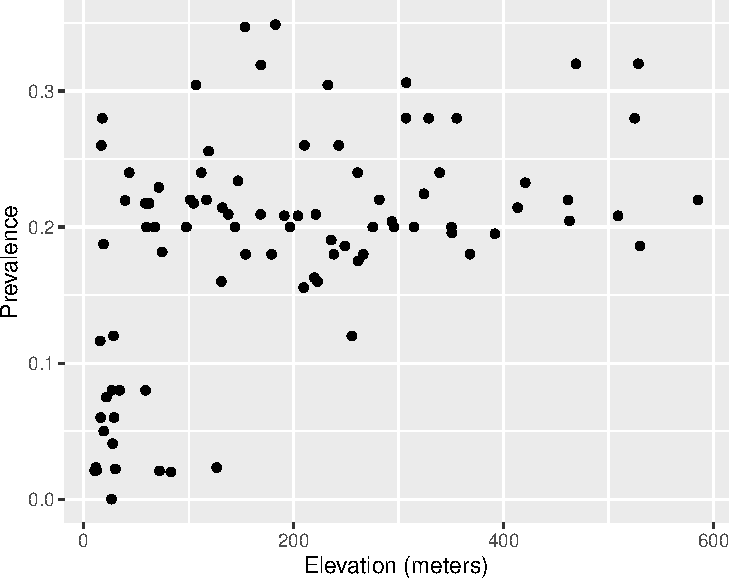
\includegraphics[keepaspectratio]{03_model-fitting_files/figure-pdf/fig-prev-elev-liberia-1.pdf}}

}

\caption{\label{fig-prev-elev-liberia}Scatter plot of the empirical
prevalence for river-blindess against elevation, measured in meters.}

\end{figure}%

The plot shown in Figure~\ref{fig-prev-elev-liberia} shows that, as
elevation increases from 0 to around 150 meters, prevalence rapidly
increases to around 0.25 and, for larger values in elevation than 150
meters, the relationship levels off. This begs the question of how we
can account for this in a regression model. To answer this question
rigorously, however, the plot in Figure~\ref{fig-prev-elev-liberia}
cannot be used. This is because, when the modelled outcome is a bounded
Binomial count, regression relationships are specified on the
logit-transformed prevalence (log-odds) scale; see Table~\ref{tbl-glm}
in Section Section~\ref{sec-geostat-models} . To explore regression
relationships in the case of prevalence data, it is convenient to use
the so-called empirical logit in place of the empirical prevalence. The
empirical logit is defined as

\begin{equation}\phantomsection\label{eq-empirical-logit}{
l_{i} = \log\left\{\frac{y_i + 1/2}{n_i - y_i + 1/2}\right\}
}\end{equation}

where \(y_i\) are the number of individuals who tested positive for
river-blindness and \(n_i\) is the total number of people tested at a
location. The reason for using the empirical logit, rather than the
standard logit transformation applied directly to the empirical
prevalence, is that it allows to generate finite values for empirical
prevalence values of 0 and 1, for which the standard logit
transformation is not defined.

\begin{Shaded}
\begin{Highlighting}[]
\CommentTok{\# The empirical logit}
\NormalTok{liberia}\SpecialCharTok{$}\NormalTok{elogit }\OtherTok{\textless{}{-}} \FunctionTok{log}\NormalTok{((liberia}\SpecialCharTok{$}\NormalTok{npos}\FloatTok{+0.5}\NormalTok{)}\SpecialCharTok{/}
\NormalTok{                      (liberia}\SpecialCharTok{$}\NormalTok{ntest}\SpecialCharTok{{-}}\NormalTok{liberia}\SpecialCharTok{$}\NormalTok{npos}\FloatTok{+0.5}\NormalTok{))}

\FunctionTok{ggplot}\NormalTok{(liberia, }\FunctionTok{aes}\NormalTok{(}\AttributeTok{x =}\NormalTok{ elevation, }\AttributeTok{y =}\NormalTok{ elogit)) }\SpecialCharTok{+} \FunctionTok{geom\_point}\NormalTok{() }\SpecialCharTok{+}
  
  \CommentTok{\# Adding a smoothing spline}
  \FunctionTok{labs}\NormalTok{(}\AttributeTok{x=}\StringTok{"Elevation (meters)"}\NormalTok{,}\AttributeTok{y=}\StringTok{"Empirical logit"}\NormalTok{) }\SpecialCharTok{+}
  \FunctionTok{stat\_smooth}\NormalTok{(}\AttributeTok{method =} \StringTok{"gam"}\NormalTok{, }\AttributeTok{formula =}\NormalTok{ y }\SpecialCharTok{\textasciitilde{}} \FunctionTok{s}\NormalTok{(x),}\AttributeTok{se=}\ConstantTok{FALSE}\NormalTok{)}\SpecialCharTok{+}
  
  \CommentTok{\# Adding linear regression fit with log{-}transformed elevation}
  \FunctionTok{stat\_smooth}\NormalTok{(}\AttributeTok{method =} \StringTok{"lm"}\NormalTok{, }\AttributeTok{formula =}\NormalTok{ y }\SpecialCharTok{\textasciitilde{}} \FunctionTok{log}\NormalTok{(x),}
              \AttributeTok{col=}\StringTok{"green"}\NormalTok{,}\AttributeTok{lty=}\StringTok{"dashed"}\NormalTok{,}\AttributeTok{se=}\ConstantTok{FALSE}\NormalTok{) }\SpecialCharTok{+}

  \CommentTok{\# Adding linear regression fit with change point in 150 meters}
  \FunctionTok{stat\_smooth}\NormalTok{(}\AttributeTok{method =} \StringTok{"lm"}\NormalTok{, }\AttributeTok{formula =}\NormalTok{ y }\SpecialCharTok{\textasciitilde{}}\NormalTok{ x }\SpecialCharTok{+} \FunctionTok{pmax}\NormalTok{(x}\DecValTok{{-}150}\NormalTok{, }\DecValTok{0}\NormalTok{),}
              \AttributeTok{col=}\StringTok{"red"}\NormalTok{,}\AttributeTok{lty=}\StringTok{"dashed"}\NormalTok{,}\AttributeTok{se=}\ConstantTok{FALSE}\NormalTok{) }
  
\end{Highlighting}
\end{Shaded}

\begin{figure}[H]

\centering{

\pandocbounded{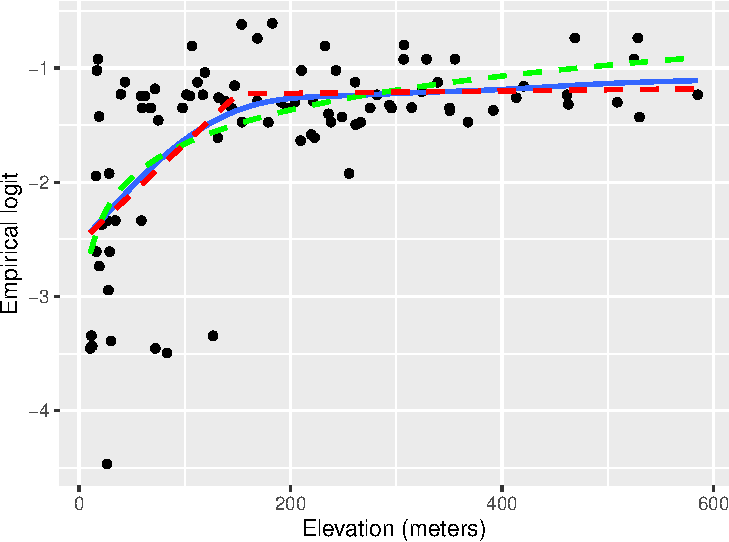
\includegraphics[keepaspectratio]{03_model-fitting_files/figure-pdf/fig-elogit-elev-liberia-1.pdf}}

}

\caption{\label{fig-elogit-elev-liberia}Scatter plot of the empirical
prevalence for river-blindess against elevation, measured in meters.}

\end{figure}%

Figure~\ref{fig-elogit-elev-liberia} shows the scatter plot of the
empirical logit against elevation. In this plot, we have also added
three lines though the \texttt{stat\_smooth} from the \texttt{ggplot2}
package. Using this function, we first pass the term \texttt{gam} to
\texttt{method} to add a penalized smoothing spline (Hastie, Tibshirani,
and Friedman 2001), represented by the blue solid line. The smoothing
spline allows us to better discern how the type of relationship and how
to best capture it using a standard regression approach. As er can see
from Figure~\ref{fig-elogit-elev-liberia}, the smoothing spline
corroborates our initial observation of a positive relationship up to
about 150 meters, followed by a plateau.

To capture this non-linear relationship, we can use the two following
approaches. The first is based on a simple log-transformation of
elevation and is represented in Figure~\ref{fig-elogit-elev-liberia} by
the green line. If were to express this relationship using a standard
Binomial regression model, this would take the form
\begin{equation}\phantomsection\label{eq-log-elev-glm}{
\log\left\{\frac{p(x_i)}{1-p(x_i)}\right\} = \beta_0 + \beta_1 \log\{e(x_i)\}
}\end{equation} where \(p(x_i)\) and \(e(x_i)\) are the river-blindness
prevalence and elevation at sampled location \(x_i\), respectively.

Alternatively, the non-linear effect of elevation on prevalence could be
captured using a linear spline. Put in simple terms, we want to fit a
linear regression model that allows for a change in slope above 150
meters. Formally, this is expressed in a Binomial regression model as
\begin{equation}\phantomsection\label{eq-lspline-elev-glm}{
\log\left\{\frac{p(x_i)}{1-p(x_i)}\right\} = \beta_0 + \beta_1 e(x_i) + \beta_{2} \max\{e(x_i)-150, 0\}.
}\end{equation} Based on the equation above, the effect of elevation
below 150 meters is quantified by the parameter \(\beta_1\). Above 150
meters, instead, the effect of elevation becomes \(\beta_1 + \beta_2\).
Note that the function \texttt{pmax} (and not the standard base function
\texttt{max}) should be used in R when the computation of the maximum
between a scalar value and each of the components of a numeric vector is
required.

Before proceeding further, it is important to explain the differences
between the use of the logarithmic transformation
(Equation~\ref{eq-log-elev-glm}) and the linear spline
(Equation~\ref{eq-lspline-elev-glm}). We observe that both curves
provide a similar fit to the data, with larger differences observed for
larger values in elevation, where the log-transformed elevation models
yields larger values for the predicted prevalence. This also suggests
that if we were to extrapolate the predictions beyond 600 meters in
elevation the implied pattern by the model with the log-transformed
elevation would predict an increasingly larger elevation, which is
unrealistic, since the fly that transmits the diseases cannot breed at
those altitudes. The linear spline model instead would generate
predictions that would be very similar to those observed between 150 and
600 meters. From this point view, the linear spline model would thus
have more scientific validity than the other model. However, which of
the two approaches should be chosen to model the effect of elevation is
a question that closely depends on the research question to be
addressed.

If the interest of the study was in better understanding the association
between elevation and prevalence, the linear spline model does not only
provide a more credible explanation but also its regression parameters
can be more easily interpreted. In fact, for a unit increase in
elevation, the multiplicative change in the odds for river-blindness is
\(\exp\{\beta_1\}\), if elevation is below 150 meters, and
\(\exp\{\beta_1+\beta_2\}\), if elevation is above 150 meters. When
instead we use the log-transformed elevation, the interpretation of
\(\beta_1\) in Equation~\ref{eq-log-elev-glm} is slightly more
complicated, as it is based on the multiplicative increase in elevation
by the same amount given by the base of the algorithm, which is about
\(e \approx 2.718\). To avoid this, one could rescale the regression
coefficient as, for example, \(\beta_1/\log_{2}(e)\) which would be
interpreted as the multiplicative change in the odds for river-blindness
for a doubling in elevation. However, a doubling in elevation is less
meaningful when considering larger values of elevation.

\begin{tcolorbox}[enhanced jigsaw, leftrule=.75mm, rightrule=.15mm, breakable, opacityback=0, coltitle=black, toprule=.15mm, toptitle=1mm, colbacktitle=quarto-callout-note-color!10!white, bottomrule=.15mm, opacitybacktitle=0.6, arc=.35mm, colback=white, title=\textcolor{quarto-callout-note-color}{\faInfo}\hspace{0.5em}{Note}, colframe=quarto-callout-note-color-frame, titlerule=0mm, bottomtitle=1mm, left=2mm]

The letter \(e\) stands for the so called Euler's number and represents
the base of the natural logarithm. In the book, we write \(\log(\cdot)\)
to mean the ``natural logarithm of \(\cdot\)''.

\end{tcolorbox}

When the goal of statistical analysis is instead in developing a
predictive model for the outcome of interest, the explanatory power and
interpretability of the model may be of less concern. For this reason,
the model with the log-transformed model could be preferred over the
model with the linear spline, if it shown to yield more predictive
power. We will come back to this point again in
Chapter~\ref{sec-geo-prediction}, where will show how to assess and
compare the predictive performance of different geostatistical models.

The other type of aggregated count data that we consider are unbounded
counts. The Anopheles mosquitoes data-set
(Section~\ref{sec-mosq-data-ch1}) is an example of this, since there is
no upper limit to the number of mosquitoes that can be trapped at a
location. Let us consider the covariate represented by elevation. In
this case, the simplest model that can be used to analyse the data is a
Poisson regression, where the linear predictor is defined on the log of
the mean number of mosquitoes (Table~\ref{tbl-glm}). Hence, exploratory
plots for the association with covariates should be generated using the
log transformed counts of mosquitoes. In this instance, to avoid taking
the log of zero, we can add 1 to the reported counts, if required. The
variable of the \texttt{An.gambiae} in the \texttt{anopheles} data-set
does not contain any 0, hence we simply apply the log tranformation
without adding 1.

\begin{Shaded}
\begin{Highlighting}[]
\NormalTok{anopheles}\SpecialCharTok{$}\NormalTok{log\_counts }\OtherTok{\textless{}{-}} \FunctionTok{log}\NormalTok{(anopheles}\SpecialCharTok{$}\NormalTok{An.gambiae)}
\FunctionTok{ggplot}\NormalTok{(anopheles, }\FunctionTok{aes}\NormalTok{(}\AttributeTok{x =}\NormalTok{ elevation, }\AttributeTok{y =}\NormalTok{ log\_counts)) }\SpecialCharTok{+} \FunctionTok{geom\_point}\NormalTok{() }\SpecialCharTok{+}
  
  \CommentTok{\# Adding a smoothing spline}
  \FunctionTok{labs}\NormalTok{(}\AttributeTok{x=}\StringTok{"Elevation (meters)"}\NormalTok{,}\AttributeTok{y=}\StringTok{"Log number of An. gambiae mosquitoes"}\NormalTok{) }\SpecialCharTok{+}
  \FunctionTok{stat\_smooth}\NormalTok{(}\AttributeTok{method =} \StringTok{"lm"}\NormalTok{, }\AttributeTok{formula =}\NormalTok{ y }\SpecialCharTok{\textasciitilde{}}\NormalTok{ x, }\AttributeTok{se=}\ConstantTok{FALSE}\NormalTok{)}
\end{Highlighting}
\end{Shaded}

\begin{figure}[H]

\centering{

\pandocbounded{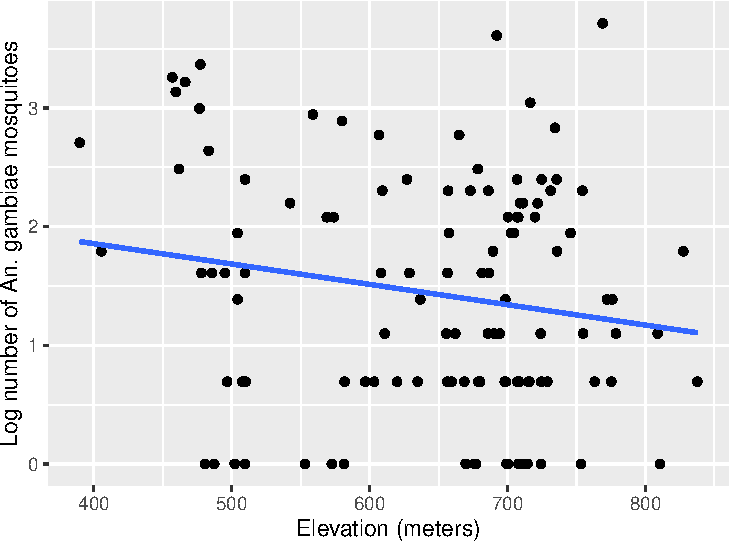
\includegraphics[keepaspectratio]{03_model-fitting_files/figure-pdf/fig-logcounts-elev-mosq-1.pdf}}

}

\caption{\label{fig-logcounts-elev-mosq}Scatter plot of the log
tranformed number of \emph{Anopheles gambiae} mosquitoes against
elevation, measured in meters. The blue line is generated using the
least squares fit.}

\end{figure}%

The scatter plot of Figure~\ref{fig-logcounts-elev-mosq} shows that
there is a negative, though weak, association, with the average number
of mosquitoes decreasing for increasing elevation. In this instance, the
assumption of a linear relationship with elevation would be a reasonable
choice.

\subsubsection{When the outcome is an invidual-level binary
indicator}\label{sec-indiv-expl-analysis}

We now consider the malaria data from Kenya
(Section~\ref{sec-malaria-ch1}) where the main outcome is the result
from a rapid diagnostic test (RDT) for malaria from individuals within
households. In this case, because the outcome only takes two values, 1
for a positive RDT test result and 0 otherwise, the direct application
of the empirical logit from Equation~\ref{eq-empirical-logit} would not
help us to generate informative scatter plots. Throughout the book, we
will consider the data from the community survey only, hence we work
with a subset of the data which we shall name \texttt{malkenya\_comm}

\begin{Shaded}
\begin{Highlighting}[]
\NormalTok{malkenya\_comm }\OtherTok{\textless{}{-}}\NormalTok{ malkenya[malkenya}\SpecialCharTok{$}\NormalTok{Survey}\SpecialCharTok{==}\StringTok{"community"}\NormalTok{, ]}
\end{Highlighting}
\end{Shaded}

To show how this issue can be overcome, let us consider the variables
age and gender. To generate a plot that can help us understand between
the relationship with malaria prevalence and the two risk factors, we
proceed as follows.

\begin{Shaded}
\begin{Highlighting}[]
\CommentTok{\# Grouping of ages into classes defined through "breaks"}
\NormalTok{malkenya\_comm}\SpecialCharTok{$}\NormalTok{Age\_class }\OtherTok{\textless{}{-}} \FunctionTok{cut}\NormalTok{(malkenya\_comm}\SpecialCharTok{$}\NormalTok{Age, }
                            \AttributeTok{breaks =} \FunctionTok{c}\NormalTok{(}\DecValTok{0}\NormalTok{, }\DecValTok{5}\NormalTok{, }\DecValTok{10}\NormalTok{, }\DecValTok{15}\NormalTok{, }\DecValTok{30}\NormalTok{, }\DecValTok{40}\NormalTok{, }\DecValTok{50}\NormalTok{, }\DecValTok{100}\NormalTok{),}
                            \AttributeTok{include.lowest =} \ConstantTok{TRUE}\NormalTok{)}
\end{Highlighting}
\end{Shaded}

Using the \texttt{cut} function, we first split age (in years) into
classes through the argument \texttt{breaks}. The classification of age
into \([0,5]\), \((5, 10]\) and \((10, 15]\) is common in many malaria
epidemiology studies, as children are one of the groups at highest risk
malaria. The choice of the other classes of age reflects instead the
need to balance the number of observations falling in each of the
classes.

\begin{Shaded}
\begin{Highlighting}[]
\CommentTok{\# Computation of the empirical logit by age groups and gender}
\NormalTok{age\_class\_data }\OtherTok{\textless{}{-}} \FunctionTok{aggregate}\NormalTok{(RDT }\SpecialCharTok{\textasciitilde{}}\NormalTok{ Age\_class }\SpecialCharTok{+}\NormalTok{ Gender, }
                                    \AttributeTok{data =}\NormalTok{ malkenya\_comm, }
                                    \AttributeTok{FUN =} \ControlFlowTok{function}\NormalTok{(y) }
                                    \FunctionTok{log}\NormalTok{((}\FunctionTok{sum}\NormalTok{(y)}\SpecialCharTok{+}\FloatTok{0.5}\NormalTok{)}\SpecialCharTok{/}\NormalTok{(}\FunctionTok{length}\NormalTok{(y)}\SpecialCharTok{{-}}\FunctionTok{sum}\NormalTok{(y)}\SpecialCharTok{+}\FloatTok{0.5}\NormalTok{)))}
\end{Highlighting}
\end{Shaded}

We then compute the empirical logit, using the total number of cases
within age group and by gender. For a given age group and gender, which
we denote as \(\mathcal{C}\), the empirical logit in
Equation~\ref{eq-empirical-logit}, now takes the form
\begin{equation}\phantomsection\label{eq-empirical-logit-bin}{
l_{\mathcal{C}} = \log\left\{\frac{\sum_{i \in \mathcal{C}} y_{i} + 0.5}{|\mathcal{C}|- \sum_{i \in \mathcal{C}} y_{i} + 0.5} \right\}
}\end{equation} where \(y_i\) are the individual binary outcomes and
\(i\in \mathcal{C}\) is used to indicate that the sum is carried out
over all the individuals who belong the class \(\mathcal{C}\),
identified by a specific age group and gender. Finally,
\(|\mathcal{C}|\) is the number of individuals who fall within
\(\mathcal{C}\). In the code above, the empirical logit in
Equation~\ref{eq-empirical-logit-bin} is computed using the
\texttt{aggregate} function. An inspection of the object
\texttt{age\_class\_data}, a data frame, shows that the empirical is
found in the column named \texttt{RDT}.

\begin{Shaded}
\begin{Highlighting}[]
\CommentTok{\# Computation of the average age within each age group }
\NormalTok{age\_class\_data}\SpecialCharTok{$}\NormalTok{age\_mean\_point }\OtherTok{\textless{}{-}} \FunctionTok{aggregate}\NormalTok{(Age }\SpecialCharTok{\textasciitilde{}}\NormalTok{ Age\_class }\SpecialCharTok{+}\NormalTok{ Gender, }
                                 \AttributeTok{data =}\NormalTok{ malkenya\_comm, }
                                 \AttributeTok{FUN =}\NormalTok{ mean)}\SpecialCharTok{$}\NormalTok{Age}


\CommentTok{\# Number of individuals within each age group, by gender}
\NormalTok{age\_class\_data}\SpecialCharTok{$}\NormalTok{n\_obs }\OtherTok{\textless{}{-}}  \FunctionTok{aggregate}\NormalTok{(Age }\SpecialCharTok{\textasciitilde{}}\NormalTok{ Age\_class }\SpecialCharTok{+}\NormalTok{ Gender, }
                         \AttributeTok{data =}\NormalTok{ malkenya\_comm, }
                         \AttributeTok{FUN =}\NormalTok{ length)}\SpecialCharTok{$}\NormalTok{Age}
\end{Highlighting}
\end{Shaded}

In order to generate the scatter-plot, we compute the average age within
each age group by gender, and use these as our values for the x-axis.
Note that since we only need to obtain the average age from this output,
we use \texttt{\$Age} to extract this only and allocate to the column
\texttt{age\_mean\_point}. Finally, we also compute the number of
observations within each of classes and place this in \texttt{n\_obs}.

\begin{Shaded}
\begin{Highlighting}[]
\FunctionTok{ggplot}\NormalTok{(age\_class\_data, }\FunctionTok{aes}\NormalTok{(}\AttributeTok{x =}\NormalTok{ age\_mean\_point, }\AttributeTok{y =}\NormalTok{ RDT, }
                           \AttributeTok{size =}\NormalTok{ n\_obs, }
                           \AttributeTok{colour =}\NormalTok{ Gender)) }\SpecialCharTok{+} 
  \FunctionTok{geom\_point}\NormalTok{() }\SpecialCharTok{+} 
  \FunctionTok{labs}\NormalTok{(}\AttributeTok{x=}\StringTok{"Age (years)"}\NormalTok{,}\AttributeTok{y=}\StringTok{"Empirical logit"}\NormalTok{)  }
\end{Highlighting}
\end{Shaded}

\begin{figure}[H]

\centering{

\pandocbounded{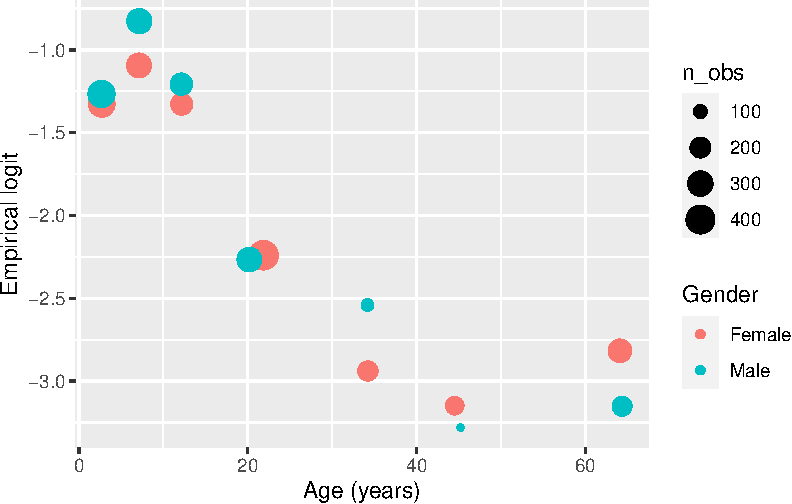
\includegraphics[keepaspectratio]{03_model-fitting_files/figure-pdf/fig-elogit-age-malkenya-1.pdf}}

}

\caption{\label{fig-elogit-age-malkenya}Plot of the empirical logit
against age, for males and females. The size of each solid point is
rendered proportional to the number of individuals within age group, as
indicated in the legend.}

\end{figure}%

The resulting plot in Figure~\ref{fig-elogit-age-malkenya} shows the
empirical logit against age by gender, with the size of each of the
points proportional to the number of observations falling within each
class. The observed patterns are explained by the fact that young
children, especially those under the age of five, are particularly
vulnerable to severe malaria infections. This is primarily due to their
immature immune systems and lack of acquired immunity. As individuals
grow older, they generally develop partial immunity to malaria through
repeated exposure to the disease. This acquired immunity can provide
some level of protection against severe malaria. At the same time,
gender roles and activities can influence exposure to malaria-carrying
mosquitoes. For example, men may spend more time outdoors for work or
other activities, increasing their exposure to mosquito bites and thus
their risk of infection. In addition, there are also biological factors
to consider. Hormonal and genetic differences between males and females
may also contribute to variations in immune responses to malaria
infection. The interaction between age and gender is complex and may
vary depending on the specific context and population being studied. A
2020 report from the Bill \& Melinda Gates foundation provides a
detailed overview of this and other aspects related to gender and
malaria (Katz and Bill \& Melinda Gates Foundation 2020).

To account for age in a model for malaria prevalence, several approaches
are possible, some of which have been developed using biological models
(Smith et al. 2007). To model the patterns observed in
Figure~\ref{fig-elogit-age-malkenya}, we can follow the same approach
used in the previous section to model the relationship between elevation
and river-blindness prevalence. First, let us consider age without the
effect of gender. Let \(p_{j}(x_i)\) denote the probability of a
positive RDT for the \(j\)-th individual living in a household at
location \(x_i\). Assuming that malaria risk reaches its peak at 15
years of age, we can capture the non-linear relationship using a linear
spline with two knots, one at 15 years and a second one at 40 years.
This is expressed as
\begin{equation}\phantomsection\label{eq-age-only-reg}{
\begin{aligned}
\log\left\{\frac{p_{j}(x_i)}{1-p_j(x_i)}\right\} = \beta_{0} + \beta_{1}a_{ij}+\beta_{2} \times\max\{a_{ij}-15, 0\} + \beta_{3}\max\{a_{ij}-40, 0\}
\end{aligned}
}\end{equation} where \(a_{ij}\) is the age, in years, for the \(j\)-th
individual at household \(i\). Based on this model the effect of age on
RDT prevalence is \(\beta_{1}\), for \(a_{ij} < 15\),
\(\beta_{1}+\beta_{2}\), for \(15 < a_{ij} < 40\), and
\(\beta_{1}+\beta_{2}+\beta_{3}\) for \(a_{ij} > 40\).

Figure~\ref{fig-elogit-age-malkenya} indicates that age may interact
with gender, meaning that the effect of gender on RDT prevalence changes
across age, with larger differences observed between males and females
for ages above 20 years. To assess such differences using a standard
Binomial regression model, the linear predictor for RDT prevalence can
be formulated as
\begin{equation}\phantomsection\label{eq-age-inter-reg}{
\begin{aligned}
\log\left\{\frac{p_{j}(x_i)}{1-p_j(x_i)}\right\} = \beta_{0} + (\beta_{1} + \beta_{1}^*g_{ij})\times a_{ij}+(\beta_{2} + \beta_{2}^*g_{ij})\times\max\{a_{ij}-15, 0\} + \\
(\beta_{3} + \beta_{3}^*g_{ij}) \times \max\{a_{ij}-40, 0\}
\end{aligned}
}\end{equation} where \(g_{ij}\) is the indicator for gender, with 1
corresponding to male and 0 to female. The coefficients \(\beta_{1}^*\),
\(\beta_{2}^*\) and \(\beta_{3}^*\) thus quantify the differences in
risk between the two genders for ages below 15 years, betwee 15 and 40
years, and above 40 years, respectively. If all of those coefficients
were 0, the model in Equation~\ref{eq-age-only-reg} would be recovered.

\begin{Shaded}
\begin{Highlighting}[]
\NormalTok{glm\_age\_gender\_interaction }\OtherTok{\textless{}{-}} \FunctionTok{glm}\NormalTok{(RDT }\SpecialCharTok{\textasciitilde{}}\NormalTok{ Age }\SpecialCharTok{+}\NormalTok{ Gender}\SpecialCharTok{:}\NormalTok{Age }\SpecialCharTok{+} 
                                  \FunctionTok{pmax}\NormalTok{(Age}\DecValTok{{-}15}\NormalTok{, }\DecValTok{0}\NormalTok{) }\SpecialCharTok{+}\NormalTok{ Gender}\SpecialCharTok{:}\FunctionTok{pmax}\NormalTok{(Age}\DecValTok{{-}15}\NormalTok{, }\DecValTok{0}\NormalTok{) }\SpecialCharTok{+} 
                                  \FunctionTok{pmax}\NormalTok{(Age}\DecValTok{{-}40}\NormalTok{, }\DecValTok{0}\NormalTok{) }\SpecialCharTok{+}\NormalTok{ Gender}\SpecialCharTok{:}\FunctionTok{pmax}\NormalTok{(Age}\DecValTok{{-}40}\NormalTok{, }\DecValTok{0}\NormalTok{),}
                              \AttributeTok{data =}\NormalTok{ malkenya\_comm, }\AttributeTok{family =}\NormalTok{ binomial)}

\FunctionTok{summary}\NormalTok{(glm\_age\_gender\_interaction)}
\DocumentationTok{\#\# }
\DocumentationTok{\#\# Call:}
\DocumentationTok{\#\# glm(formula = RDT \textasciitilde{} Age + Gender:Age + pmax(Age {-} 15, 0) + Gender:pmax(Age {-} }
\DocumentationTok{\#\#     15, 0) + pmax(Age {-} 40, 0) + Gender:pmax(Age {-} 40, 0), family = binomial, }
\DocumentationTok{\#\#     data = malkenya\_comm)}
\DocumentationTok{\#\# }
\DocumentationTok{\#\# Coefficients:}
\DocumentationTok{\#\#                              Estimate Std. Error z value Pr(\textgreater{}|z|)    }
\DocumentationTok{\#\# (Intercept)                  {-}1.05835    0.10245 {-}10.331  \textless{} 2e{-}16 ***}
\DocumentationTok{\#\# Age                          {-}0.03384    0.01310  {-}2.584  0.00978 ** }
\DocumentationTok{\#\# pmax(Age {-} 15, 0)            {-}0.03975    0.02356  {-}1.687  0.09162 .  }
\DocumentationTok{\#\# pmax(Age {-} 40, 0)             0.09170    0.02482   3.695  0.00022 ***}
\DocumentationTok{\#\# Age:GenderMale                0.01428    0.01221   1.170  0.24202    }
\DocumentationTok{\#\# GenderMale:pmax(Age {-} 15, 0) {-}0.03625    0.03145  {-}1.153  0.24908    }
\DocumentationTok{\#\# GenderMale:pmax(Age {-} 40, 0)  0.02451    0.04320   0.567  0.57052    }
\DocumentationTok{\#\# {-}{-}{-}}
\DocumentationTok{\#\# Signif. codes:  0 \textquotesingle{}***\textquotesingle{} 0.001 \textquotesingle{}**\textquotesingle{} 0.01 \textquotesingle{}*\textquotesingle{} 0.05 \textquotesingle{}.\textquotesingle{} 0.1 \textquotesingle{} \textquotesingle{} 1}
\DocumentationTok{\#\# }
\DocumentationTok{\#\# (Dispersion parameter for binomial family taken to be 1)}
\DocumentationTok{\#\# }
\DocumentationTok{\#\#     Null deviance: 2875.8  on 3351  degrees of freedom}
\DocumentationTok{\#\# Residual deviance: 2673.8  on 3345  degrees of freedom}
\DocumentationTok{\#\# AIC: 2687.8}
\DocumentationTok{\#\# }
\DocumentationTok{\#\# Number of Fisher Scoring iterations: 5}
\end{Highlighting}
\end{Shaded}

The code above shows how to fit the model specified in
Equation~\ref{eq-age-inter-reg}. The terms \texttt{Age},
\texttt{pmax(Age-15,\ 0)} and \texttt{pmax(Age-40,\ 0)} respectively
correspond to \(\beta_{1}\), \(\beta_{2}\) and \(\beta_{3}\), whilst the
\texttt{Gender:Age}, \texttt{Gender:pmax(Age-15,\ 0)} and
\texttt{Gender:pmax(Age-40,\ 0)} to \(\beta_{1}^*\), \(\beta_{2}^*\) and
\(\beta_{3}^*\), respectively. In the summary of the fitted model, we
observe that the interaction coefficients are non-statistically
significant. However, removing the interaction based on the fact that
each of the coefficients have each p-values larger than the conventional
level of 5\% would be wrong. Instead we should carry out the likelihood
ratio test, as shown below.

\begin{Shaded}
\begin{Highlighting}[]
\NormalTok{glm\_age\_gender\_no\_interaction }\OtherTok{\textless{}{-}} \FunctionTok{glm}\NormalTok{(RDT }\SpecialCharTok{\textasciitilde{}}\NormalTok{ Age }\SpecialCharTok{+}  \FunctionTok{pmax}\NormalTok{(Age}\DecValTok{{-}15}\NormalTok{, }\DecValTok{0}\NormalTok{) }\SpecialCharTok{+} \FunctionTok{pmax}\NormalTok{(Age}\DecValTok{{-}40}\NormalTok{, }\DecValTok{0}\NormalTok{),}
                              \AttributeTok{data =}\NormalTok{ malkenya\_comm, }\AttributeTok{family =}\NormalTok{ binomial)}

\FunctionTok{anova}\NormalTok{(glm\_age\_gender\_no\_interaction, glm\_age\_gender\_interaction, }\AttributeTok{test =} \StringTok{"Chisq"}\NormalTok{)}
\DocumentationTok{\#\# Analysis of Deviance Table}
\DocumentationTok{\#\# }
\DocumentationTok{\#\# Model 1: RDT \textasciitilde{} Age + pmax(Age {-} 15, 0) + pmax(Age {-} 40, 0)}
\DocumentationTok{\#\# Model 2: RDT \textasciitilde{} Age + Gender:Age + pmax(Age {-} 15, 0) + Gender:pmax(Age {-} }
\DocumentationTok{\#\#     15, 0) + pmax(Age {-} 40, 0) + Gender:pmax(Age {-} 40, 0)}
\DocumentationTok{\#\#   Resid. Df Resid. Dev Df Deviance Pr(\textgreater{}Chi)}
\DocumentationTok{\#\# 1      3348     2675.6                     }
\DocumentationTok{\#\# 2      3345     2673.8  3   1.8051   0.6138}
\end{Highlighting}
\end{Shaded}

To carry out the likelihood ratio test to assess the null hypothesis
that \(\beta_{1}^*=\beta_{2}^*=\beta_{3}^*=0\), we first fit the
simplified nested model under this null hypothesis. The likelihood ratio
test can then be carried out using the \texttt{anova} command as shown.
The p-value indicates that the we do not find evidence against the null
hypothesis, hence in our analysis of the data we might favour the
simplified model that does not assumes an interaction between the two
genders.

The approach just illustrated, can also be applied to explore the
association with other continuous variables that are a property of the
household and not of the individual. Let us, for example, consider the
variable \texttt{elevation} from the \texttt{malkenya} data-set.

\begin{Shaded}
\begin{Highlighting}[]
\NormalTok{malkenya\_comm}\SpecialCharTok{$}\NormalTok{elevation\_class }\OtherTok{\textless{}{-}} \FunctionTok{cut}\NormalTok{(malkenya\_comm}\SpecialCharTok{$}\NormalTok{elevation,}
                            \AttributeTok{breaks =} \FunctionTok{quantile}\NormalTok{(malkenya\_comm}\SpecialCharTok{$}\NormalTok{elevation, }\FunctionTok{seq}\NormalTok{(}\DecValTok{0}\NormalTok{, }\DecValTok{1}\NormalTok{, }\AttributeTok{by =} \FloatTok{0.1}\NormalTok{)),}
                            \AttributeTok{include.lowest =} \ConstantTok{TRUE}\NormalTok{)}
\end{Highlighting}
\end{Shaded}

Following the same approach used for age, we first split elevation into
classes. To define these, we use the deciles of the empirical
distribution of \texttt{elevation} which we calculate using the
\texttt{quantile} function above. In this way we also ensure that the
number of observations falling within each class of elevation is
approximately the same.

\begin{Shaded}
\begin{Highlighting}[]
\CommentTok{\# Computation of the empirical logit by classes of elevation}
\NormalTok{elev\_class\_data }\OtherTok{\textless{}{-}} \FunctionTok{aggregate}\NormalTok{(RDT }\SpecialCharTok{\textasciitilde{}}\NormalTok{ elevation\_class, }
                                    \AttributeTok{data =}\NormalTok{ malkenya\_comm, }
                                    \AttributeTok{FUN =} \ControlFlowTok{function}\NormalTok{(y) }
                                    \FunctionTok{log}\NormalTok{((}\FunctionTok{sum}\NormalTok{(y)}\SpecialCharTok{+}\FloatTok{0.5}\NormalTok{)}\SpecialCharTok{/}\NormalTok{(}\FunctionTok{length}\NormalTok{(y)}\SpecialCharTok{{-}}\FunctionTok{sum}\NormalTok{(y)}\SpecialCharTok{+}\FloatTok{0.5}\NormalTok{)))}


\CommentTok{\# Computation of the average elevation within each class of elevation}
\NormalTok{elev\_class\_data}\SpecialCharTok{$}\NormalTok{elevation\_mean }\OtherTok{\textless{}{-}} \FunctionTok{aggregate}\NormalTok{(elevation }\SpecialCharTok{\textasciitilde{}}\NormalTok{ elevation\_class, }
                                    \AttributeTok{data =}\NormalTok{ malkenya\_comm, }
                                    \AttributeTok{FUN =}\NormalTok{ mean)}\SpecialCharTok{$}\NormalTok{elevation}
\end{Highlighting}
\end{Shaded}

We then compute the empirical logit and the average elevation for each
class of elevation. The empirical logit is computed as already defined
in Equation~\ref{eq-empirical-logit-bin}, where now the definition of
\(\mathcal{C}\) is given by a specific decile used to split the
distribution of elevation.

\begin{Shaded}
\begin{Highlighting}[]
\FunctionTok{ggplot}\NormalTok{(elev\_class\_data, }\FunctionTok{aes}\NormalTok{(}\AttributeTok{x =}\NormalTok{ elevation\_mean, }\AttributeTok{y =}\NormalTok{ RDT), }
                           \AttributeTok{size =}\NormalTok{ n\_obs) }\SpecialCharTok{+} 
  \FunctionTok{geom\_point}\NormalTok{() }\SpecialCharTok{+} 
  \FunctionTok{labs}\NormalTok{(}\AttributeTok{x=}\StringTok{"Elevation (meters)"}\NormalTok{,}\AttributeTok{y=}\StringTok{"Empirical logit"}\NormalTok{)  }
\end{Highlighting}
\end{Shaded}

\begin{figure}[H]

\centering{

\pandocbounded{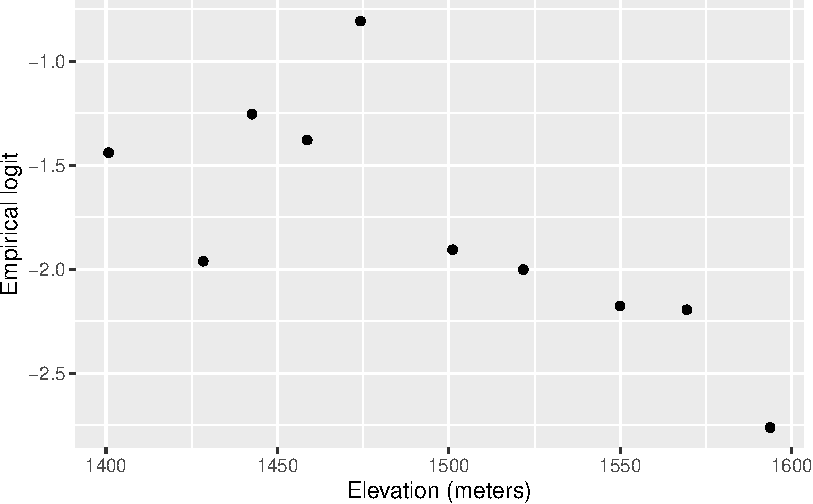
\includegraphics[keepaspectratio]{03_model-fitting_files/figure-pdf/fig-elogit-elev-malkenya-1.pdf}}

}

\caption{\label{fig-elogit-elev-malkenya}Plot of the empirical logit
against elevation measured in meters.}

\end{figure}%

The resulting plot in Figure~\ref{fig-elogit-elev-malkenya} shows an
approximately linear relationship with decreasing values of the
empirical logit for increasing elevation. This is expected because the
cooler environment at higher altitudes is less favourable to the
development of the overall mosquito life cycle.

An alternative approach to generate a scatter plot for assessing the
association between elevation and the empirical logit would be to
aggregate the data at household level, rather than using classes of
elevation. However, this approach does not work as the one illustrated
above when only one individual is sampled for each location. In the case
of the \texttt{malkenya} data, the great majority of the locations only
include one individual making this second approach less useful than the
one illustrated.

Other more sophisticated approaches for the exploration of the
associations between covariates and binary outcomes are available. For
example, the use of the empirical logit could be avoided by using
non-parametric regression methods for Binomial outcomes (Bowman 1997),
also implemented in \texttt{sm} package in R. Our view is that a careful
exploratory analysis based on simpler methods, as those illustrated
above, can be equally effective to inform the module formulation.

\subsection{Exploring overdispersion in count
data}\label{sec-overdispersion}

One of the main advantages in the use of covariates is the ability to
attribute part of the variation of the outcome to a set of measured
variables and, hence, reduce the uncertainty of our inferences. However,
it almost always the case that the finite number of covariates at our
disposal is not enough to fully explain the variation in the outcome. In
other words, the existence of unmeasured covariates that are related to
the modelled outcome give rise to the so called residual variation. In a
standard linear regression model the extent to which we are able to
account for important covariates is directly linked to the size of the
variance of the residuals. In the case of count data, instead, this link
is less well defined and one of the main consequences of the omission of
covariates, which we address in this chapter, is \emph{overdispersion}.

Overdispersion occurs when the variability of the data is larger than
that implied by the generalized linear model (GLM) fitted to them. For
example, if we consider the Binomial distribution, the presence of
overdispersion implies that \(V(Y_i) > n_i \mu_{i}(1-\mu_i)\), where we
recall that \(n_i\) is the Binomial denominator and \(mu_i\) is the
probability of ``success'' for each of the \(n_i\) Bernoulli trials; for
a Poisson distribution with \(E(Y_i) = \mu_i\), instead, overdispersion
implies that \(V(Y_i) > \mu_{i}\).

Assessment of the overdispersion for count data can be carried out in
different ways depending on the goal of the statistical analysis. Since
the focus of this book is to illustrate how to formulate and apply
geostatistical models, the most natural approach to assess
overdispersion is through the use of generalized linear mixed models
(GLMMs). The class of GLMMs that we consider in this and the next
section are obtained by replacing the spatial Gaussian process
\(S(x_i)\) in introduced in Equation~\ref{eq-linear-predictor-ch1} with
a set of mutually independent random effects, which we denote as
\(Z_i\), and thus write
\begin{equation}\phantomsection\label{eq-linear-predictor-glmms-ch2}{
g(\mu_i) = d(x_i)^\top \beta + Z_i.
}\end{equation} The model above accounts for the overdispersion in the
data through \(Z_i\) whose variance can be interpreted as an indicator
of the amount of overdispersion. To show this, we carry out a small
simulation as follows. For simplicity, we consider the Binomial mixed
model with an intercept only, hence
\begin{equation}\phantomsection\label{eq-bin-glmm-example}{
\log\left\{\frac{\mu_i}{1-\mu_i}\right\} = \beta_0 + Z_i
}\end{equation} and assume that the \(Z_i\) follow a set of mutually
independent Gaussian variables with mean 0 and variance \(\tau^2\). In
our simulation we vary \(\beta_0\) over the set
\(\{-3, -2, -1, 0, 1, 2, 3\}\) and set \(\tau^2=0.1\) and the binomial
denominators to \(n_i = 100\). For a given value of \(\beta_0\), we then
proceed through the following iterative steps.

\begin{itemize}
\item
  Simulate 10,000 values for \(Z_i\) from a Gaussian distribution with
  mean 0 and variance \(\tau^2\).
\item
  Compute the probabilities \(\mu_i\) based on
  Equation~\ref{eq-bin-glmm-example}.
\item
  Simulate 10,000 values from a Binomial model with probability of
  success \(\mu_i\) and denominator \(n_i\).
\item
  Compute the empirical variance of the counts \(y_i\) simulated in the
  previous step.
\item
  Change the value of \(\beta_0\) and repeat the previous steps, for all
  the values of \(\beta_0\).
\end{itemize}

The code below shows the implementation of the above steps in R.

\begin{Shaded}
\begin{Highlighting}[]
\CommentTok{\# Number of simulations}
\NormalTok{n\_sim }\OtherTok{\textless{}{-}} \DecValTok{10000}

\CommentTok{\# Variance of the Z\_i}
\NormalTok{tau2 }\OtherTok{\textless{}{-}} \FloatTok{0.1}

\CommentTok{\# Binomial denominator }
\NormalTok{bin\_denom }\OtherTok{\textless{}{-}} \DecValTok{100}

\CommentTok{\# Intercept values}
\NormalTok{beta0 }\OtherTok{\textless{}{-}} \FunctionTok{c}\NormalTok{(}\SpecialCharTok{{-}}\DecValTok{3}\NormalTok{, }\SpecialCharTok{{-}}\DecValTok{2}\NormalTok{, }\SpecialCharTok{{-}}\DecValTok{1}\NormalTok{, }\DecValTok{0}\NormalTok{, }\DecValTok{1}\NormalTok{, }\DecValTok{2}\NormalTok{, }\DecValTok{3}\NormalTok{)}

\CommentTok{\# Vector where we store the computed variance from}
\CommentTok{\# the simulated counts from the Binomial mixed model}
\NormalTok{var\_data }\OtherTok{\textless{}{-}} \FunctionTok{rep}\NormalTok{(}\ConstantTok{NA}\NormalTok{, }\FunctionTok{length}\NormalTok{(beta0))}


\ControlFlowTok{for}\NormalTok{(j }\ControlFlowTok{in} \DecValTok{1}\SpecialCharTok{:}\FunctionTok{length}\NormalTok{(beta0)) \{}
  \CommentTok{\# Simulation of the random effects Z\_i}
\NormalTok{  Z\_i\_sim }\OtherTok{\textless{}{-}} \FunctionTok{rnorm}\NormalTok{(n\_sim, }\AttributeTok{sd =} \FunctionTok{sqrt}\NormalTok{(tau2))}

  \CommentTok{\# Linear predictor of the Binomial mixed model}
\NormalTok{  lp }\OtherTok{\textless{}{-}}\NormalTok{ beta0[j]  }\SpecialCharTok{+}\NormalTok{ Z\_i\_sim}
  
  \CommentTok{\# Probabilities of the Binomial distribution conditional on Z\_i}
\NormalTok{  prob\_sim }\OtherTok{\textless{}{-}} \FunctionTok{exp}\NormalTok{(lp)}\SpecialCharTok{/}\NormalTok{(}\DecValTok{1}\SpecialCharTok{+}\FunctionTok{exp}\NormalTok{(lp))}
  
  \CommentTok{\# Simulation of the counts from the Binomial mixed model}
\NormalTok{  y\_i\_sim }\OtherTok{\textless{}{-}} \FunctionTok{rbinom}\NormalTok{(n\_sim, }\AttributeTok{size =}\NormalTok{ bin\_denom, }\AttributeTok{prob =}\NormalTok{ prob\_sim)}
  
  \CommentTok{\# Empirical variance from the simulated counts}
\NormalTok{  var\_data[j] }\OtherTok{\textless{}{-}} \FunctionTok{var}\NormalTok{(y\_i\_sim)}
\NormalTok{\}}

\CommentTok{\# Probabilities from the standard Binomial model (Z\_i = 0)}
\NormalTok{probs\_binomial }\OtherTok{\textless{}{-}} \FunctionTok{exp}\NormalTok{(beta0)}\SpecialCharTok{/}\NormalTok{(}\DecValTok{1}\SpecialCharTok{+}\FunctionTok{exp}\NormalTok{(beta0))}

\CommentTok{\# Variance from the standard Binomial model}
\NormalTok{var\_bimomial }\OtherTok{\textless{}{-}}\NormalTok{ bin\_denom}\SpecialCharTok{*}\NormalTok{probs\_binomial}\SpecialCharTok{*}\NormalTok{(}\DecValTok{1}\SpecialCharTok{{-}}\NormalTok{probs\_binomial)}
\end{Highlighting}
\end{Shaded}

\begin{Shaded}
\begin{Highlighting}[]
\NormalTok{plot\_df }\OtherTok{\textless{}{-}} \FunctionTok{data.frame}\NormalTok{(}
  \AttributeTok{beta0 =}\NormalTok{ beta0,}
  \StringTok{\textasciigrave{}}\AttributeTok{Binomial mixed model}\StringTok{\textasciigrave{}}   \OtherTok{=}\NormalTok{ var\_data,}
  \StringTok{\textasciigrave{}}\AttributeTok{Standard Binomial model}\StringTok{\textasciigrave{}}\OtherTok{=} \ControlFlowTok{if}\NormalTok{ (}\FunctionTok{exists}\NormalTok{(}\StringTok{"var\_binomial"}\NormalTok{)) var\_binomial }\ControlFlowTok{else}\NormalTok{ var\_bimomial}
\NormalTok{)}

\NormalTok{df\_long }\OtherTok{\textless{}{-}}\NormalTok{ tidyr}\SpecialCharTok{::}\FunctionTok{pivot\_longer}\NormalTok{(}
\NormalTok{  plot\_df,}
  \AttributeTok{cols =} \FunctionTok{c}\NormalTok{(Binomial.mixed.model, Standard.Binomial.model),}
  \AttributeTok{names\_to =} \StringTok{"Model"}\NormalTok{,}
  \AttributeTok{values\_to =} \StringTok{"Variance"}
\NormalTok{)}

\CommentTok{\# Pretty legend labels}
\NormalTok{df\_long}\SpecialCharTok{$}\NormalTok{Model }\OtherTok{\textless{}{-}} \FunctionTok{factor}\NormalTok{(}
\NormalTok{  df\_long}\SpecialCharTok{$}\NormalTok{Model,}
  \AttributeTok{levels =} \FunctionTok{c}\NormalTok{(}\StringTok{"Binomial.mixed.model"}\NormalTok{, }\StringTok{"Standard.Binomial.model"}\NormalTok{),}
  \AttributeTok{labels =} \FunctionTok{c}\NormalTok{(}\StringTok{"Binomial mixed model"}\NormalTok{, }\StringTok{"Standard Binomial model"}\NormalTok{)}
\NormalTok{)}

\FunctionTok{ggplot}\NormalTok{(df\_long, }\FunctionTok{aes}\NormalTok{(}\AttributeTok{x =}\NormalTok{ beta0, }\AttributeTok{y =}\NormalTok{ Variance, }\AttributeTok{color =}\NormalTok{ Model)) }\SpecialCharTok{+}
  \FunctionTok{geom\_point}\NormalTok{() }\SpecialCharTok{+}
  \FunctionTok{geom\_line}\NormalTok{() }\SpecialCharTok{+}
  \FunctionTok{labs}\NormalTok{(}\AttributeTok{x =} \FunctionTok{expression}\NormalTok{(beta[}\DecValTok{0}\NormalTok{]), }\AttributeTok{y =} \StringTok{"Variance"}\NormalTok{) }\SpecialCharTok{+}
  \FunctionTok{theme\_minimal}\NormalTok{() }\SpecialCharTok{+}
  \FunctionTok{theme}\NormalTok{(}\AttributeTok{legend.title =} \FunctionTok{element\_blank}\NormalTok{(),}
        \AttributeTok{legend.position =} \FunctionTok{c}\NormalTok{(}\FloatTok{0.2}\NormalTok{, }\FloatTok{0.85}\NormalTok{))}
\end{Highlighting}
\end{Shaded}

\begin{figure}[H]

\centering{

\pandocbounded{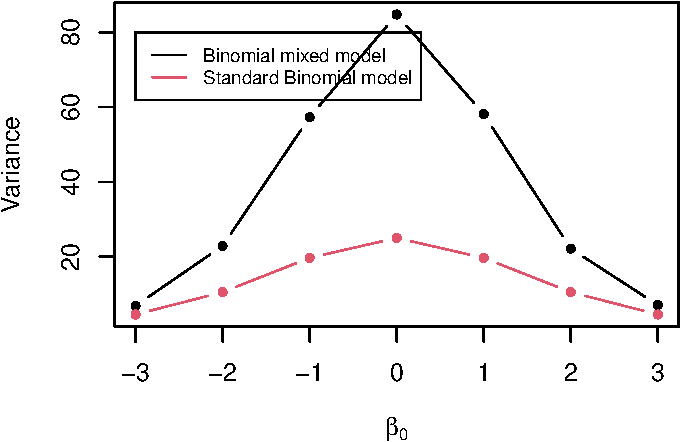
\includegraphics[keepaspectratio]{03_model-fitting_files/figure-pdf/fig-var-bin-glmm-1.pdf}}

}

\caption{\label{fig-var-bin-glmm}Plot of the variances of the standard
Binomial model and the Binomial mixed model (see
Equation~\ref{eq-bin-glmm-example}) against \(\beta_0\)}

\end{figure}%

Figure~\ref{fig-var-bin-glmm} shows the results of the simulation. In
this figure, the red line corresponds to the variance of a standard
Binomial model, obtained by setting \(Z_i=0\) and computed as
\(n_i \mu_i (1-\mu_i)\) with
\(\mu_i = \exp\{\beta_0\}/(1+\exp\{\beta_0\})\). As expected, this plot
shows that the variance of the simulated counts from the mixed model in
Equation~\ref{eq-bin-glmm-example} exhibit a larger variance than would
be expected under the standard Binomial model. It also indicates that
the chosen value for the variance of \(Z_i\) of \(\tau^2 = 0.1\)
corresponds to a significant amount of dispersion. One way to relate
\(\tau^2\) to the amount of overdispersion is by considering that,
following from the properties of a univariate Gaussian distribution,
\emph{a priori} the \(Z_i\) will take values between
\(-1.96 \sqrt{\tau^2}\) and \(+1.96 \sqrt{\tau^2}\) with approximately
95\(\%\) probability. That implies that \(\exp\{Z_i\}\), which expresses
the effect of the random effects on the odds ratios, will be with
95\(\%\) probability between \(\exp\{-1.96 \sqrt{\tau^2}\}\) and
\(\exp\{+1.96 \sqrt{\tau^2}\}\). By replacing \(\tau^2\) with the chosen
values for the simulation, those two becomes about 0.54 and 1.86,
meaning that with the \(Z_i\) with \(95\%\) probability will have a
multiplicative effect on the odds ratios between \(0.54\) and \(1.86\).

We encourage you to do Exercise 1 and Exercise 2 at the end of this
chapter, to further explore how generalized linear mixed models can be
used as a tool to account for overdispersion.

\subsubsection{Maximum likelihood estimation of generalized linear mixed
models for count
data}\label{maximum-likelihood-estimation-of-generalized-linear-mixed-models-for-count-data}

We now illustrate how to fit a generalize linear mixed, using the
\texttt{anopheles} data-set as an example. We consider two models: an
intercept-only model and one that uses elevation as a covariate. Let
\(\mu(x_i)\) be the number of mosquitoes captured at a location \(x_i\);
then the linear predictor with elevation as a covariate takes the form
\begin{equation}\phantomsection\label{eq-anopheles-glmm}{
\log\{\mu_i\} = \beta_{0} + \beta_{1} d(x_i) + Z_i
}\end{equation} where \(d(x_i)\) indicates the elevation in meters at
location \(x_i\) and the \(Z_i\) are independent and identically
distributed Gaussian variables with mean 0 and variance \(\tau^2\). The
model with an intercept only is simply obtained by setting
\(\beta_1 = 0\).

We carry out the estimation in R using the \texttt{glmer} function from
the \texttt{lme4} package (see Bates et al. (2015) for a detailed
tutorial). The \texttt{glmer} function implements the maximum likelihood
estimation for generalized linear mixed models. The code below shows how
the \texttt{glmer} is used to carry out this step for the model in
Equation~\ref{eq-anopheles-glmm} and the one withuot covariates.

\begin{Shaded}
\begin{Highlighting}[]
\CommentTok{\# Create the ID of the location}
\NormalTok{anopheles}\SpecialCharTok{$}\NormalTok{ID\_loc }\OtherTok{\textless{}{-}} \DecValTok{1}\SpecialCharTok{:}\FunctionTok{nrow}\NormalTok{(anopheles)}

\CommentTok{\# Poisson mixed model with elevation}
\NormalTok{fit\_glmer\_elev }\OtherTok{\textless{}{-}} \FunctionTok{glmer}\NormalTok{(An.gambiae }\SpecialCharTok{\textasciitilde{}} \FunctionTok{scale}\NormalTok{(elevation) }\SpecialCharTok{+}\NormalTok{ (}\DecValTok{1}\SpecialCharTok{|}\NormalTok{ID\_loc), }\AttributeTok{family =}\NormalTok{ poisson, }
                        \AttributeTok{data =}\NormalTok{ anopheles, }\AttributeTok{nAGQ =} \DecValTok{25}\NormalTok{)}

\CommentTok{\# Poisson mixed model with intercept only}
\NormalTok{fit\_glmer\_int }\OtherTok{\textless{}{-}} \FunctionTok{glmer}\NormalTok{(An.gambiae }\SpecialCharTok{\textasciitilde{}}\NormalTok{ (}\DecValTok{1}\SpecialCharTok{|}\NormalTok{ID\_loc), }\AttributeTok{family =}\NormalTok{ poisson, }
                        \AttributeTok{data =}\NormalTok{ anopheles, }\AttributeTok{nAGQ =} \DecValTok{25}\NormalTok{)}
\end{Highlighting}
\end{Shaded}

To fit the model with \texttt{glmer}, we first must create a variable in
our data-set that allows us to identify the location associated with
each count. In this case, since every row corresponds to a different
location, we simply use the row number to identify the locations and
save this in the \texttt{ID\_loc} variable. The random effects \(Z_i\)
are then included in the model by adding
\texttt{(1\ \textbar{}\ ID\_loc)} in the formula of the \texttt{glmer}
function.

When introducing the variable elevation, we standardize the variable so
that its mean is 0 and its variance is 1. This is done to aid the
convergence of the algorithm used to fit the model and it is generally
considered good practice, especially when many variables with different
scales are used as covariates. However, we emphasize that standardizing
a variable does not affect the fit of the model to the data. This is
because the model with the standardized variable is a reparametrization
of the model with the unstandardized variable. In other words, a model
that uses standardized covariates only attaches a different
interpretation to its regression coefficients while maintaining the same
goodness of fit of the model with that uses the covariates on their
original scale.

The argument \texttt{nAGQ} is used to define the precision of the
approximation of the maximum likelihood estimation algorithm. By default
\texttt{nAGQ\ =\ 1}, which corresponds to the Laplace approximation.
Values for \texttt{nAGQ} larger than 1 are used to define the number of
points of the adaptive Gaussian-Hermite quadrature. The general
principle is that the larger \texttt{nAGQ} the better, but at the
expense of an increased computing time. Based on the guidelines and help
pages of the \texttt{lme4} package, it is stated that a reasonable value
for \texttt{nAGQ} is 25. For more technical details on this aspect, we
refer the reader to Bates et al. (2015).

We can now look at the summary of the fitted models to the mosquitoes
data-set.

\begin{Shaded}
\begin{Highlighting}[]
\DocumentationTok{\#\#\# Summary of the model with elevation}
\FunctionTok{summary}\NormalTok{(fit\_glmer\_elev)}
\DocumentationTok{\#\# Generalized linear mixed model fit by maximum likelihood (Adaptive}
\DocumentationTok{\#\#   Gauss{-}Hermite Quadrature, nAGQ = 25) [glmerMod]}
\DocumentationTok{\#\#  Family: poisson  ( log )}
\DocumentationTok{\#\# Formula: An.gambiae \textasciitilde{} scale(elevation) + (1 | ID\_loc)}
\DocumentationTok{\#\#    Data: anopheles}
\DocumentationTok{\#\# }
\DocumentationTok{\#\#       AIC       BIC    logLik {-}2*log(L)  df.resid }
\DocumentationTok{\#\#     291.8     300.1    {-}142.9     285.8       113 }
\DocumentationTok{\#\# }
\DocumentationTok{\#\# Scaled residuals: }
\DocumentationTok{\#\#      Min       1Q   Median       3Q      Max }
\DocumentationTok{\#\# {-}0.89574 {-}0.42469 {-}0.09483  0.29445  0.53352 }
\DocumentationTok{\#\# }
\DocumentationTok{\#\# Random effects:}
\DocumentationTok{\#\#  Groups Name        Variance Std.Dev.}
\DocumentationTok{\#\#  ID\_loc (Intercept) 0.7146   0.8453  }
\DocumentationTok{\#\# Number of obs: 116, groups:  ID\_loc, 116}
\DocumentationTok{\#\# }
\DocumentationTok{\#\# Fixed effects:}
\DocumentationTok{\#\#                  Estimate Std. Error z value Pr(\textgreater{}|z|)    }
\DocumentationTok{\#\# (Intercept)       1.53042    0.09365  16.342   \textless{}2e{-}16 ***}
\DocumentationTok{\#\# scale(elevation) {-}0.19794    0.08950  {-}2.212    0.027 *  }
\DocumentationTok{\#\# {-}{-}{-}}
\DocumentationTok{\#\# Signif. codes:  0 \textquotesingle{}***\textquotesingle{} 0.001 \textquotesingle{}**\textquotesingle{} 0.01 \textquotesingle{}*\textquotesingle{} 0.05 \textquotesingle{}.\textquotesingle{} 0.1 \textquotesingle{} \textquotesingle{} 1}
\DocumentationTok{\#\# }
\DocumentationTok{\#\# Correlation of Fixed Effects:}
\DocumentationTok{\#\#             (Intr)}
\DocumentationTok{\#\# scale(lvtn) 0.036}

\DocumentationTok{\#\#\# Summary of the model with the intercept only}
\FunctionTok{summary}\NormalTok{(fit\_glmer\_int)}
\DocumentationTok{\#\# Generalized linear mixed model fit by maximum likelihood (Adaptive}
\DocumentationTok{\#\#   Gauss{-}Hermite Quadrature, nAGQ = 25) [glmerMod]}
\DocumentationTok{\#\#  Family: poisson  ( log )}
\DocumentationTok{\#\# Formula: An.gambiae \textasciitilde{} (1 | ID\_loc)}
\DocumentationTok{\#\#    Data: anopheles}
\DocumentationTok{\#\# }
\DocumentationTok{\#\#       AIC       BIC    logLik {-}2*log(L)  df.resid }
\DocumentationTok{\#\#     294.6     300.1    {-}145.3     290.6       114 }
\DocumentationTok{\#\# }
\DocumentationTok{\#\# Scaled residuals: }
\DocumentationTok{\#\#      Min       1Q   Median       3Q      Max }
\DocumentationTok{\#\# {-}0.73816 {-}0.42718 {-}0.06941  0.26564  0.45022 }
\DocumentationTok{\#\# }
\DocumentationTok{\#\# Random effects:}
\DocumentationTok{\#\#  Groups Name        Variance Std.Dev.}
\DocumentationTok{\#\#  ID\_loc (Intercept) 0.761    0.8724  }
\DocumentationTok{\#\# Number of obs: 116, groups:  ID\_loc, 116}
\DocumentationTok{\#\# }
\DocumentationTok{\#\# Fixed effects:}
\DocumentationTok{\#\#             Estimate Std. Error z value Pr(\textgreater{}|z|)    }
\DocumentationTok{\#\# (Intercept)  1.52849    0.09584   15.95   \textless{}2e{-}16 ***}
\DocumentationTok{\#\# {-}{-}{-}}
\DocumentationTok{\#\# Signif. codes:  0 \textquotesingle{}***\textquotesingle{} 0.001 \textquotesingle{}**\textquotesingle{} 0.01 \textquotesingle{}*\textquotesingle{} 0.05 \textquotesingle{}.\textquotesingle{} 0.1 \textquotesingle{} \textquotesingle{} 1}
\end{Highlighting}
\end{Shaded}

From the summary of the model that uses elevation, we observe the that
the estimated regression coefficient \(\beta_{1}\) is statistically
significant different from 0. The interpretation of the estimated
regression coefficient is the following: for an increase of about 100
meters in elevation, all other things being equal, the average number of
mosquitoes decreases by about
\(100\% \times [1-\exp\{-0.19794\}] \approx 18\%\). Note that when using
a standardized variable, a unit increase for this corresponds to an
increase in the original unstandardized variable equal to its standard
deviation, which for the \texttt{elevation} variable is about 100
meters.

From the summaries of the two models, under \texttt{Random\ effects:},
we obtain the estimates associates with the random effects introduced in
the model. In this case, since we only have introduced \(Z_i\), this
part of summary provides the maximum likelihood estimate for \(\tau^2\),
the variance of \(Z_i\), which found on the line where \texttt{ID\_loc}
is printed. We then observe that the estimates for \(\tau^2\) for the
intercept-only model is \texttt{0.761}, whilst for the model with
elevation this is \texttt{0.7146}. Note that the figures reported under
\texttt{Std.Dev.} are simply the square root of the value reported under
\texttt{Variance}. As expected, the introduction of elevation
contributes to the explanation of the residual variation captured by
\(Z_i\), though by a very small amount. The estimated values of
\(\tau^2\) thus suggest that there is extra-Binomial variation in the
data that is not account for by elevation.

In the next section, we will illustrate how to assess the presence of
residual correlation for continuous measurements and overdispersed count
data.

\subsection{Exploring residual spatial
correlation}\label{sec-expl-spatial}

In its most basic form, the concept of spatial correlation can be
succinctly encapsulated by Tobler (1970) first law of geography, which
posits that ``everything is interconnected, but objects in close
proximity exhibit stronger relationships than those situated farther
apart.'' After we have identified the key variables to introduce as
covariates in the model (Section~\ref{sec-expl-assoc}) and, in the case
of count data, assessed the presence of overdispersion
(Section~\ref{sec-overdispersion}), our final exploratory step consists
of assessing whether the residuals of the non spatial model show
evidence of spatial correlation. Hence, in geostatistical modelling, the
interest is not in the spatial correlation of the data, but rather on
understanding whether the variation in the outcome unexplained by the
covariates exhibits spatial correlation. We call this \emph{residual
spatial correlation}, to emphasize that spatial correlation is a concept
relative to the covariates that we have introduced in the model.

In the context of geostatistical analysis, the tool that is generally
used to assess the residual spatial correlation is the the so called
\emph{empirical variogram}. Before looking at the mathematical
definition of the empirical variogram, let us consider a generalized
linear mixed model as expressed in
Equation~\ref{eq-linear-predictor-glmms-ch2}. Our goal is then to
question the assumption of independently distributed random effects
\(Z_i\) by asking whether the \(Z_i\) show evidence of spatial
correlation. Let \(Z_i\) and \(Z_j\) be two random effects that are
associate with two different locations \(x_i\) and \(x_j\),
respectively, and let us take the squared difference between the two
\begin{equation}\phantomsection\label{eq-squared-diff}{
V_{ij} = (Z_i - Z_j)^2.
}\end{equation} How does the spatial correlation affect the value of
\(V_{ij}\)? To answer this question, we can refer to the aforementioned
Tobler's law of geography. When \(x_i\) and \(x_j\) will be closer to
each other, then \(Z_i\) and \(Z_j\) will also tend to be more similar
to each other, thus making \(V_{ij}\) smaller, on average. On the
contrary, when \(x_i\) and \(x_j\) will be further apart, then
\(V_{ij}\) will become larger, on average. We can then construct the
empirical variogram by considering all possible pairs of locations
\(x_i\) and \(x_j\), for which we then compute \(V_{ij}\) and plot this
against the distance between \(x_i\) and \(x_j\), which we denote as
\(u_{ij}\). If there is spatial correlation in the random effects
\(Z_i\), then this will manifest as an average increase in the
\(V_{ij}\) as \(u_{ij}\) increases. However, there are still two issues
that we have to address before we can generate and plot the empirical
variogram.

The first issue is that we do not observe \(Z_i\) as, by definition,
this is a latent variable. Hence, we require an estimate for \(Z_i\)
which we can then feed into \(V_{ij}\). To emphasize this point, from
now on, we shall replace Equation~\ref{eq-squared-diff} with
\begin{equation}\phantomsection\label{eq-hat-squared-diff}{
\hat{V}_{ij} = (\hat{Z}_{i} - \hat{Z}_j)^2.
}\end{equation} Several options are available for estimating \(Z_{i}\).
Our choice is to use the model of the predictive distribution of
\(Z_i\), that is the distribution of \(Z_{i}\) conditioned to the data
\(y_i\). This estimator for \(Z_i\) is also readily available from the
output of the \texttt{lmer} and \texttt{glmer} functions of the
\texttt{lme4} package, as we will illustrate later in our example in
this section.

The second issue is that if simply plot \(\hat{V}_{ij}\) against the
distances \(u_{ij}\) (also knwon as \emph{cloud variogram}), due to the
high noiseness in the \(\hat{V}_{ij}\), it may be quite difficult to
assess the presence of an increasing trend in the \(\hat{V}_{ij}\) and
thus detect spatial correlation. Hence, it is general practice to group
the distances \(u_{ij}\) into classes, say \(\mathcal{U}\), and then
take average of all the \(\hat{V}_{ij}\) that fall within
\(\mathcal{U}\).

We can now write the formal definition of the empirical variogram as
\begin{equation}\phantomsection\label{eq-empirical-variogram}{
\hat{V}(\mathcal{U}) = \frac{1}{2 |\mathcal{U}|} \sum_{(i, j): (u_i, u_j) \in \mathcal{U}} \hat{V}_{ij}
}\end{equation} where \(|\mathcal{U}|\) denotes the number of pairs of
locations that fall within the distance class \(\mathcal{U}\). The
rationale behind dividing by 2 in \(1/2 |\mathcal{U}|\) from the above
equation, will be elucidated in Section~\ref{sec-linear-model}, and
there is no need for us to delve into this matter at this juncture. When
creating the empirical variogram plot, we select the midpoint values of
the distance classes \(\mathcal{U}\) to represent the x-axis values.

Before we can evaluate residual spatial correlation, there remains one
crucial concern: relying solely on a visual inspection of the empirical
variogram is susceptible to human subjectivity. Furthermore, it is worth
noting that even a seemingly upward trend observed in the empirical
variogram might be merely a product of random fluctuations, rather than
a reliable indication of actual residual spatial correlation. To address
these concerns and enhance the objectivity of the use of the empirical
variogram, one approach would involve comparing the observed empirical
variogram pattern with those generated in the absence of spatial
correlation. Following this principle, we then use a permutation test
that allows us to generate empirical variograms under the assumption of
absence of spatial correlation through the following iterative steps.

\begin{enumerate}
\def\labelenumi{\arabic{enumi}.}
\item
  Permute the order of the locations in the data-set while keeping
  everything else fixed.
\item
  Compute the empirical variogram \(\hat{V}(\mathcal{U})\) for the
  permuted data-set.
\item
  Repeat 1 and 2 a large number of times, say 10,000.
\item
  Use the resulting 10,000 empirical varigorams to compute 95\(\%\)
  confidence intervals, by taking the 0.025 and 0.975 quantiles of these
  for each distance class \(\hat{V}(\mathcal{U})\).
\item
  If the observed empirical variogram falls fully within the envelope
  generated in the previous point, we then conclude that the data do not
  exhibit residual spatial correlation. If, instead, the observed
  empirical variogram partly falls outside the envelope we conclude that
  the data do exhibit residual spatial correlation.
\end{enumerate}

We now show an application of all the concepts introduced in this
section to the Liberia data on river-blindness.

\subsubsection{Example: assessing spatial correlation for the Liberia
data}\label{sec-empirical-variog-bin}

We consider the Binomial mixed model that uses the log-transformed
elevation as a covariate to model river blindness prevalence, hence
\begin{equation}\phantomsection\label{eq-liberia-bin-mixed-elev}{
\log\left\{\frac{p(x_i)}{1-p(x_i)}\right\} = \beta_{0} + \beta_{1}\log\{e(x_i)\} + Z_i
}\end{equation} where \(e(x_i)\) is the elevation in meters at location
\(x_i\) and the \(Z_i\) are i.i.d. Gaussian variables with mean 0 and
variance \(\tau^2\). We first fit the model above using the
\texttt{glmer} function.

\begin{Shaded}
\begin{Highlighting}[]
\CommentTok{\# Convert the data{-}set into an sf object}
\NormalTok{liberia }\OtherTok{\textless{}{-}} \FunctionTok{st\_as\_sf}\NormalTok{(liberia, }\AttributeTok{coords =} \FunctionTok{c}\NormalTok{(}\StringTok{"lat"}\NormalTok{, }\StringTok{"long"}\NormalTok{), }\AttributeTok{crs =} \DecValTok{4326}\NormalTok{)}


\CommentTok{\# Create the ID of the location}
\NormalTok{liberia}\SpecialCharTok{$}\NormalTok{ID\_loc }\OtherTok{\textless{}{-}} \DecValTok{1}\SpecialCharTok{:}\FunctionTok{nrow}\NormalTok{(liberia)}

\CommentTok{\# Binomial mixed model with log{-}elevation}
\NormalTok{fit\_glmer\_lib }\OtherTok{\textless{}{-}} \FunctionTok{glmer}\NormalTok{(}\FunctionTok{cbind}\NormalTok{(npos, ntest) }\SpecialCharTok{\textasciitilde{}} \FunctionTok{log}\NormalTok{(elevation) }\SpecialCharTok{+}\NormalTok{ (}\DecValTok{1}\SpecialCharTok{|}\NormalTok{ID\_loc), }\AttributeTok{family =}\NormalTok{ binomial,}
                        \AttributeTok{data =}\NormalTok{ liberia, }\AttributeTok{nAGQ =} \DecValTok{25}\NormalTok{)}

\FunctionTok{summary}\NormalTok{(fit\_glmer\_lib)}
\end{Highlighting}
\end{Shaded}

\begin{verbatim}
Generalized linear mixed model fit by maximum likelihood (Adaptive
  Gauss-Hermite Quadrature, nAGQ = 25) [glmerMod]
 Family: binomial  ( logit )
Formula: cbind(npos, ntest) ~ log(elevation) + (1 | ID_loc)
   Data: liberia

      AIC       BIC    logLik -2*log(L)  df.resid 
    127.9     135.4     -61.0     121.9        87 

Scaled residuals: 
     Min       1Q   Median       3Q      Max 
-2.46033 -0.63341 -0.07633  0.61995  3.12732 

Random effects:
 Groups Name        Variance Std.Dev.
 ID_loc (Intercept) 0.003097 0.05565 
Number of obs: 90, groups:  ID_loc, 90

Fixed effects:
               Estimate Std. Error z value Pr(>|z|)    
(Intercept)    -2.96292    0.21184 -13.987  < 2e-16 ***
log(elevation)  0.26143    0.04071   6.422 1.35e-10 ***
---
Signif. codes:  0 '***' 0.001 '**' 0.01 '*' 0.05 '.' 0.1 ' ' 1

Correlation of Fixed Effects:
            (Intr)
log(elevtn) -0.981
\end{verbatim}

From the output, we observe that the estimate for \(\tau^2\) is about
0.003, indicating a moderate level of overdispersion in the data.

\begin{Shaded}
\begin{Highlighting}[]
\NormalTok{liberia}\SpecialCharTok{$}\NormalTok{Z\_hat }\OtherTok{\textless{}{-}} \FunctionTok{ranef}\NormalTok{(fit\_glmer\_lib)}\SpecialCharTok{$}\NormalTok{ID\_loc[,}\DecValTok{1}\NormalTok{]}
\end{Highlighting}
\end{Shaded}

Through the function \texttt{ranef} when extract the estimates of the
random effects \(Z_i\) and save these in the data set. We then use the
function \texttt{s\_variogram} from the \texttt{RiskMap} package to
compute the empirical varigoram for the estimated \(\hat{Z}_i\).

\begin{Shaded}
\begin{Highlighting}[]
\NormalTok{liberia\_variog }\OtherTok{\textless{}{-}} \FunctionTok{s\_variogram}\NormalTok{(}\AttributeTok{data =}\NormalTok{ liberia,}
                              \AttributeTok{variable =} \StringTok{"Z\_hat"}\NormalTok{,}
                              \AttributeTok{bins =} \FunctionTok{c}\NormalTok{(}\DecValTok{15}\NormalTok{, }\DecValTok{30}\NormalTok{, }\DecValTok{40}\NormalTok{, }\DecValTok{80}\NormalTok{, }\DecValTok{120}\NormalTok{,}
                                       \DecValTok{160}\NormalTok{, }\DecValTok{200}\NormalTok{, }\DecValTok{250}\NormalTok{, }\DecValTok{300}\NormalTok{, }\DecValTok{350}\NormalTok{),}
                              \AttributeTok{scale\_to\_km =} \ConstantTok{TRUE}\NormalTok{,}
                              \AttributeTok{n\_permutation =} \DecValTok{10000}\NormalTok{)}
\end{Highlighting}
\end{Shaded}

Through the argument \texttt{bins} we can specify the the classes of
distance, previously denoted by \(\mathcal{U}\); check the help page of
\texttt{s\_variogram} to see how this is defined by default. The value
passed to \texttt{bins} in the code above correspond to define the
following classes of distance \(\mathcal{U}\): \([15, 30]\),
\((30, 40]\) and so forth, with the last class being \([350, +\infty)\),
i.e.~all pairs of locations whose distances are above 350km. The
argument \texttt{n\_permutation} allows the user to specify the number
of permutations that are performed the generate the envelope for absence
of spatial correlation previously described.

\begin{Shaded}
\begin{Highlighting}[]
\FunctionTok{dist\_summaries}\NormalTok{(}\AttributeTok{data =}\NormalTok{ liberia,}
               \AttributeTok{scale\_to\_km =} \ConstantTok{TRUE}\NormalTok{)}
\DocumentationTok{\#\# $min}
\DocumentationTok{\#\# [1] 3.204561}
\DocumentationTok{\#\# }
\DocumentationTok{\#\# $max}
\DocumentationTok{\#\# [1] 514.9768}
\DocumentationTok{\#\# }
\DocumentationTok{\#\# $mean}
\DocumentationTok{\#\# [1] 199.7156}
\DocumentationTok{\#\# }
\DocumentationTok{\#\# $median}
\DocumentationTok{\#\# [1] 185.7845}
\end{Highlighting}
\end{Shaded}

The \texttt{dist\_summaries} function within the \texttt{RiskMap}
package can be used for gauging the extent of the area covered by your
dataset, aiding in the selection of appropriate values to be passed to
the \texttt{bins} argument. In the provided output above, we can observe
that for the Liberia dataset, the minimum and maximum distances span
approximately 3km and 533km, respectively. While there is not a
one-size-fits-all recommendation for setting \texttt{bins}, two
fundamental principles should inform your decision-making. Firstly, it
is advisable to avoid choosing overly large distance intervals, as the
uncertainty associated with the empirical variogram tends to increase
with distance due to fewer available pairs of observations for
estimation. Secondly, especially when spatial correlation is not strong,
it is crucial to carefully explore the behavior of the variogram at
smaller distances. Consequently, it is generally advisable to experiment
with different \texttt{bins} configurations and observe how they impact
the pattern of the empirical variogram.

\begin{Shaded}
\begin{Highlighting}[]
\FunctionTok{plot\_s\_variogram}\NormalTok{(liberia\_variog,}
                 \AttributeTok{plot\_envelope =} \ConstantTok{TRUE}\NormalTok{)}
\end{Highlighting}
\end{Shaded}

\begin{figure}[H]

\centering{

\pandocbounded{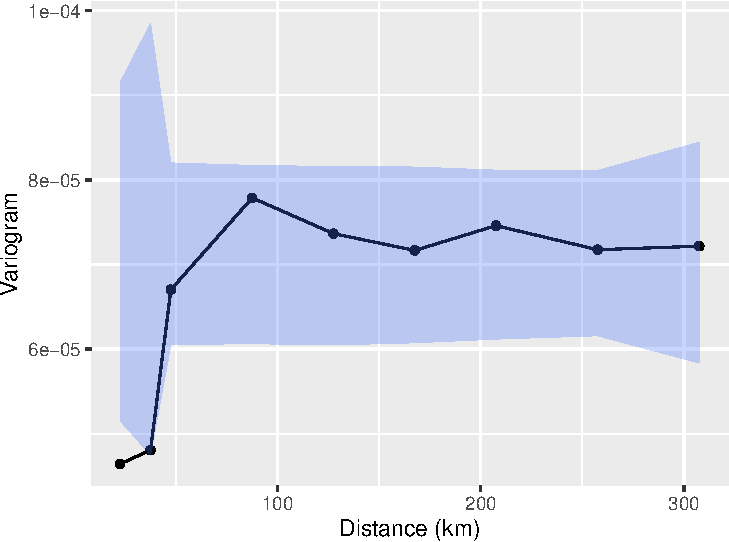
\includegraphics[keepaspectratio]{03_model-fitting_files/figure-pdf/fig-liberia-variog-1.pdf}}

}

\caption{\label{fig-liberia-variog}Plot of the empirical variogram
(solid line) computed using the estimated random effects from the model
in Equation~\ref{eq-liberia-bin-mixed-elev}. The blue shaded area is the
95\% confidence level envelope generated using the permutation procedure
described in Section~\ref{sec-expl-spatial}.}

\end{figure}%

Finally, the \texttt{plot\_s\_variogram} function enables us to
visualize the empirical variogram and, through the
\texttt{plot\_envelope} argument, include the envelope generated by the
permutation procedure. As illustrated in
Figure~\ref{fig-liberia-variog}, we observe that the empirical variogram
falls outside the envelope at relatively short distances, typically
below 30km. However, for distances exceeding 30km, the behavior of the
empirical variogram does not significantly differ from variograms
generated under the assumption of spatial independence. In summary, we
interpret the evidence presented in Figure~\ref{fig-liberia-variog} as
indicative of residual spatial correlation within the data.
Nevertheless, it is essential to exercise caution when attempting to
ascertain the scale of the spatial correlation using the empirical
variogram. As we will emphasize throughout this book, the empirical
variogram's sensitivity to the choice of bins values renders it an
unreliable tool for drawing statistical inferences. In other words, we
advocate employing the empirical variogram primarily to assess the
presence of residual correlation.

\subsubsection{Exploring residual spatial correlation with linear
Guassian models}\label{sec-empirical-variog-lm}

When using a linear model to assess spatial correlation, it is important
to distinguish two cases: 1) when the data contain only one location per
location; 2) when more than one observation per location is available.
We now consider each of these two scenarios separately.

\paragraph{One observation per
location}\label{one-observation-per-location}

To illustrate the use of the variogram under this scenario, we shall use
the Gailicia data on lead concentration in moss samples. The simplest
possible model for the data is a standard linear model without
covariates which assumes independence among the observations, hence
\begin{equation}\phantomsection\label{eq-std-lm-galicia}{
Y_i = \beta_0 + U_i
}\end{equation} where the \(U_i\) are i.i.d. Gaussian variables with
mean zero and variance \(\omega^2\). At this stage, our goal is then to
assess whether the assumption of independence for the \(Z_i\) is
supported by the data or whether there is evidence of spatial
correlation. However, the measurement error of the device may be present
as part of the natural random variation in \(Z_i\) which might mask the
detection of spatial correlation using the residuals \(Z_i\)
challenging, especially is the measurement error dominates the spatial
variation of the data. One would be tempted to introduce an additional,
location-specific random effect, say \(Z_i\) with mean zero and variance
\(\tau^2\) and fit the model
\begin{equation}\phantomsection\label{eq-std-lm2-galicia}{
Y_i = \beta_0 + Z_i + U_i,
}\end{equation} where we interpret \(U_i\) as random variation due to
the measurement device and \(Z_i\) as a random effect accounting for
unmeasured covariates that contribute to the variation between locations
in lead concentration. However, the model in
Equation~\ref{eq-std-lm2-galicia} is not identifiable because we cannot
disentangle the separate contributions of \(Z_i\) and \(U_i\) from the
variation of the data, unless: a) we know the precision of the
measurement device, \(\omega\) (recall that \(\omega^2\) is the variance
of \(U_i\)); b) or, if we do not know \(\omega\), we can then separate
the two sources of variation only if we have multiple observations per
location (the scenario which we shall consider in the next section).

For the Galicia data, for we do not know the measurement device
precision and we only have one observation per location. However, this
does not prevent us from using the variogram based on the residuals from
Equation~\ref{eq-std-lm-galicia}, while keeping in mind the limitations
and uncertainty that are inherent to this exploratory tool as remarked
at the end of the last paragraph.

\begin{Shaded}
\begin{Highlighting}[]
\CommentTok{\# Fitting of the linear model and extraction of the residuals  }
\NormalTok{lm\_fit }\OtherTok{\textless{}{-}} \FunctionTok{lm}\NormalTok{(}\FunctionTok{log}\NormalTok{(lead) }\SpecialCharTok{\textasciitilde{}} \DecValTok{1}\NormalTok{, }\AttributeTok{data =}\NormalTok{ galicia)}
\NormalTok{galicia}\SpecialCharTok{$}\NormalTok{residuals }\OtherTok{\textless{}{-}}\NormalTok{ lm\_fit}\SpecialCharTok{$}\NormalTok{residuals}

\CommentTok{\# Convert the galicia data frame into an "sf" object}
\NormalTok{galicia\_sf }\OtherTok{\textless{}{-}} \FunctionTok{st\_as\_sf}\NormalTok{(galicia, }\AttributeTok{coords =} \FunctionTok{c}\NormalTok{(}\StringTok{"x"}\NormalTok{, }\StringTok{"y"}\NormalTok{), }\AttributeTok{crs =} \DecValTok{32629}\NormalTok{)}

\CommentTok{\# Compute the variogram, using the residuals from the linear model fit,}
\CommentTok{\# and the 95\% confidence level envelope for spatial independence}
\NormalTok{galicia\_variog }\OtherTok{\textless{}{-}} \FunctionTok{s\_variogram}\NormalTok{(galicia\_sf, }\AttributeTok{variable =} \StringTok{"residuals"}\NormalTok{,}
                              \AttributeTok{scale\_to\_km =} \ConstantTok{TRUE}\NormalTok{,}
                              \AttributeTok{bins =} \FunctionTok{seq}\NormalTok{(}\DecValTok{10}\NormalTok{, }\DecValTok{140}\NormalTok{, }\AttributeTok{length =} \DecValTok{15}\NormalTok{),}
                              \AttributeTok{n\_permutation =} \DecValTok{10000}\NormalTok{)}

\CommentTok{\# Plotting the results}
\FunctionTok{plot\_s\_variogram}\NormalTok{(galicia\_variog, }\AttributeTok{plot\_envelope =} \ConstantTok{TRUE}\NormalTok{)}
\end{Highlighting}
\end{Shaded}

\begin{figure}[H]

\centering{

\pandocbounded{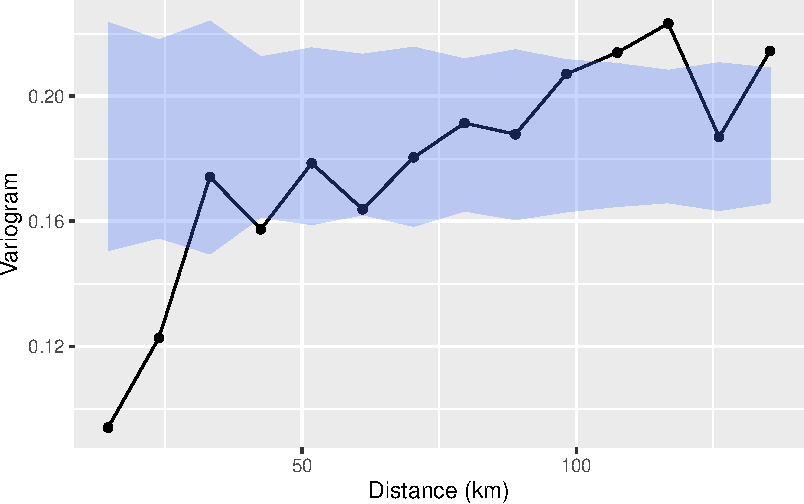
\includegraphics[keepaspectratio]{03_model-fitting_files/figure-pdf/fig-galicia-variog-1.pdf}}

}

\caption{\label{fig-galicia-variog}Plot of the empirical variogram
(solid line) computed using the estimated residuals from the model in
Equation~\ref{eq-std-lm-galicia}. The blue shaded area is the 95\%
confidence level envelope generated using the permutation procedure
described in Section~\ref{sec-expl-spatial}.}

\end{figure}%

In the code above, we first fit the linear model in
Equation~\ref{eq-std-lm-galicia} and then extract the residuals from
this. Note that for this simple model, the residuals of the model are
obtained by simply centering the outcome to zero by subtracting its
mean. However, for more complex linear models that use covariates the
computation of the residuals is more involved and can be carried out
through a simple extension of the code above by specifying an
appropriate \texttt{formula} in the \texttt{lm} function.

Figure~\ref{fig-galicia-variog} shows the empirical variogram and the
95\% envelope for spatial independence. This clearly shows that the
measurement of lead concentration are spatially correlated.

\paragraph{More than one observation per
location}\label{sec-explanal-lm}

For the case of more than one observation per location, we shall
consider the \texttt{italy\_sim} data-set. This data-set contains 10
observations per location, for a total of 200 locations. The variable
\texttt{ID\_loc} is a numeric indicator that can be used to identify the
location each observation belong to. For this data-set, we use the
population density, named \texttt{pop\_dens}, as a log-transformed
covariate; we leave you as an exercise to assess that is a reasonable
modelling choice.

To specify a non-spatial mixed model for the outcome, we then use two
subscripts: \(i\) to identify a given location; \(j\) to identify the
\(j\)-th observation for a given location \(i\). We denote as \(Z_i\)
the location-specific random effect ans as \(U_{ij}\) the random
variation due to the measurement error inherent to each observation.
Hence, we write \begin{equation}\phantomsection\label{eq-italy-sim-lmm}{
Y_{ij} = \beta_0 + \beta_1 \log\{d(x_i)\} + Z_i + U_{ij},
}\end{equation} where \(d(x_i)\) is the population density at location
\(x_i\); as before, we use \(\tau^2\) and \(\omega^2\) to denote the
variances of \(Z_i\) and \(U_{ij}\), respectively. To fit this model to
the data we use the \texttt{lmer} function from the \texttt{lme4}
package.

\begin{Shaded}
\begin{Highlighting}[]
\CommentTok{\# Fitting a linear mixed model to the italy\_sim data{-}set}
\CommentTok{\# See main text for model specification}
\NormalTok{lmer\_fit }\OtherTok{\textless{}{-}} \FunctionTok{lmer}\NormalTok{(y }\SpecialCharTok{\textasciitilde{}} \FunctionTok{log}\NormalTok{(pop\_dens) }\SpecialCharTok{+}\NormalTok{ (}\DecValTok{1}\SpecialCharTok{|}\NormalTok{ID\_loc), }\AttributeTok{data =}\NormalTok{ italy\_sim)}

\FunctionTok{summary}\NormalTok{(lmer\_fit)}
\DocumentationTok{\#\# Linear mixed model fit by REML [\textquotesingle{}lmerMod\textquotesingle{}]}
\DocumentationTok{\#\# Formula: y \textasciitilde{} log(pop\_dens) + (1 | ID\_loc)}
\DocumentationTok{\#\#    Data: italy\_sim}
\DocumentationTok{\#\# }
\DocumentationTok{\#\# REML criterion at convergence: 3390.9}
\DocumentationTok{\#\# }
\DocumentationTok{\#\# Scaled residuals: }
\DocumentationTok{\#\#      Min       1Q   Median       3Q      Max }
\DocumentationTok{\#\# {-}2.85209 {-}0.64198 {-}0.01832  0.66014  3.01870 }
\DocumentationTok{\#\# }
\DocumentationTok{\#\# Random effects:}
\DocumentationTok{\#\#  Groups   Name        Variance Std.Dev.}
\DocumentationTok{\#\#  ID\_loc   (Intercept) 2.5006   1.5813  }
\DocumentationTok{\#\#  Residual             0.1959   0.4426  }
\DocumentationTok{\#\# Number of obs: 2000, groups:  ID\_loc, 200}
\DocumentationTok{\#\# }
\DocumentationTok{\#\# Fixed effects:}
\DocumentationTok{\#\#               Estimate Std. Error t value}
\DocumentationTok{\#\# (Intercept)   {-}0.40448    0.57613  {-}0.702}
\DocumentationTok{\#\# log(pop\_dens)  1.33798    0.07643  17.506}
\DocumentationTok{\#\# }
\DocumentationTok{\#\# Correlation of Fixed Effects:}
\DocumentationTok{\#\#             (Intr)}
\DocumentationTok{\#\# log(pp\_dns) {-}0.981}

\CommentTok{\# Incorporating the estimated random effects into the data}
\NormalTok{italy\_sim}\SpecialCharTok{$}\NormalTok{rand\_eff }\OtherTok{\textless{}{-}}\FunctionTok{ranef}\NormalTok{(lmer\_fit)}\SpecialCharTok{$}\NormalTok{ID\_loc[italy\_sim}\SpecialCharTok{$}\NormalTok{ID\_loc,}\DecValTok{1}\NormalTok{]}

\CommentTok{\# Converting the italy\_sim data frame into an "sf" object }
\NormalTok{italy\_sim\_sf }\OtherTok{\textless{}{-}} \FunctionTok{st\_as\_sf}\NormalTok{(italy\_sim, }\AttributeTok{coords=}\FunctionTok{c}\NormalTok{(}\StringTok{"x1"}\NormalTok{, }\StringTok{"x2"}\NormalTok{), }\AttributeTok{crs =} \DecValTok{32634}\NormalTok{)}

\CommentTok{\# Compute the variogram, using the random effects from the linear mixed model fit,}
\CommentTok{\# and the 95\% confidence level envelope for spatial independence}
\NormalTok{italy\_sim\_variog }\OtherTok{\textless{}{-}} \FunctionTok{s\_variogram}\NormalTok{(italy\_sim\_sf, }\AttributeTok{variable =} \StringTok{"rand\_eff"}\NormalTok{, }
                                \AttributeTok{scale\_to\_km =} \ConstantTok{TRUE}\NormalTok{,}
                                \AttributeTok{n\_permutation =} \DecValTok{200}\NormalTok{)}

\CommentTok{\# Plotting the results}
\FunctionTok{plot\_s\_variogram}\NormalTok{(italy\_sim\_variog, }\AttributeTok{plot\_envelope =} \ConstantTok{TRUE}\NormalTok{)}
\end{Highlighting}
\end{Shaded}

\begin{figure}[H]

\centering{

\pandocbounded{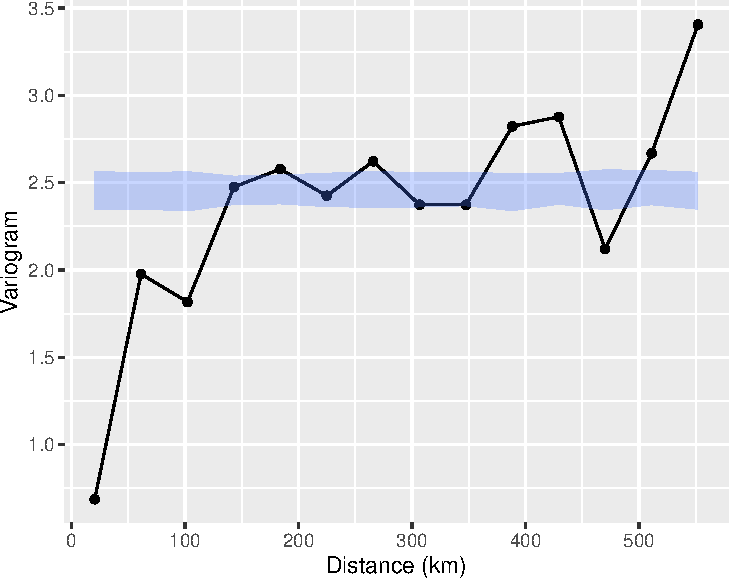
\includegraphics[keepaspectratio]{03_model-fitting_files/figure-pdf/fig-italy-sim-variog-1.pdf}}

}

\caption{\label{fig-italy-sim-variog}Plot of the empirical variogram
(solid line) computed using the estimated random effects from the model
in Equation~\ref{eq-italy-sim-lmm}. The blue shaded area is the 95\%
confidence level envelope generated using the permutation procedure
described in Section~\ref{sec-expl-spatial}.}

\end{figure}%

In the code above, the introduction of the \(Z_i\) random effect is
specified in the \texttt{lmer} function though
\texttt{(1\textbar{}ID\_loc)} in the formula; recall that
\texttt{ID\_loc} is the numerical indicator that identifies each
location. From the summary of the model, we obtain both the estimates of
the regression coefficients \(\beta_{0}\) and \(\beta_{1}\), as well for
the variances \(\tau^2\) listed under \texttt{Random\ effects:}. The
estimate of \(\sigma^2\) is found on the line of printed output starting
with \texttt{ID\_loc}, whilst that for \$\omega\^{}2 is next to
\texttt{Residual}.

The application of the empirical variogram, whose results are shown in
Figure~\ref{fig-italy-sim-variog}, indicate the presence of residual
correlation. This is because we observe that the solid line representing
the empirical variogram falls outside of the 95\% envelope for spatial
independence.

\section{The linear geostatistical model}\label{sec-linear-model}

In this section, we consider spatially referenced outcomes \(Y_i\) that
are continuous. We first consider the simpler case of a single
measurement \(Y_i\) per location \(x_i\). Recalling the class of
generalized linear models introduced in
Section~\ref{sec-geostat-models}, the linear predictor takes the form
\begin{equation}\phantomsection\label{eq-linear-geostat-model-lp}{
\mu_{i} = d(x_i)^\top \beta + S(x_i).
}\end{equation} Hence, in this case, we interpret \(\beta\) as the
effect on \(\mu_i\) for a unit increase in \(d(x_i)\). Let \(U_i\)
denote i.i.d. random variables representing the measurement error
associated with \(Y_i\), each having mean zero and variance
\(\omega^2\). Thanks to the linear properties of Gaussian random
variables, we can also express the linear model in a compact expression,
as \begin{equation}\phantomsection\label{eq-linear-geostat-model}{
Y_i = \mu_i + U_i = d(x_i)^\top \beta + S(x_i) + U_i.
}\end{equation} To fully specify a geostatistical model for our dataset,
we must address two critical aspects.

\begin{enumerate}
\def\labelenumi{\arabic{enumi}.}
\tightlist
\item
  Defining the relationship between each covariate and the mean value
  \(\mu_i\).
\item
  Selecting an appropriate correlation function for \(S(x)\).
\end{enumerate}

As illustrated in the previous sections, the initial step of exploratory
analysis allows us to handle the first aspect, where we determine the
regression relationship between covariates and the mean value \(\mu_i\).
However, based on existing methods of exploratory analysis, it is
difficult to understand what is a suitable correlation function at this
stage. A commonly recommended starting point is the Matern correlation
function (see Equation~\ref{eq-matern}), which offers considerable
flexibility in capturing a wide range of correlation structures, under
the assumption stationarity and isotropy. As we shall illustrate in the
next example, even estimating a Matern correlation function is a task
that poses many inferential challenges due to the poor identifiability,
especially, of its smoothness parameter \(\kappa\).

\subsection{\texorpdfstring{Evaluating the inclusion of the measurement
error term \(U_i\) and the specification of the smoothness parameter
\(\kappa\)}{Evaluating the inclusion of the measurement error term U\_i and the specification of the smoothness parameter \textbackslash kappa}}\label{sec-glm-parest}

In this section we analyse the Galicia data using a linear
geostatistical geostatitsical model for the log-transformed lead
concentration, which we denote as \(Y_i\). Since we do not use
covariates, we then write the model as
\begin{equation}\phantomsection\label{eq-galicia-lgm}{
Y_i = \mu + S(x_i) + U_i
}\end{equation} where were \(S(x)\) is a Matern process with variance
\(\sigma^2\), scale parameter \(\phi\) and and smothness parameter
\(\kappa\); the \(U_i\) correspond to the measurement error term and
denote with \(\omega^2\) their variance.

We carry out the parameter estimation of the model using the
\texttt{glgpm} function from the \texttt{RiskMap} package. This function
implements maximum likelihood estimation for generalized linear mixed
models using a Matern correlation function, while fixing the smoothness
parameter \(\kappa\) at prespecified value by the user. The object
passed to the argument \texttt{data} in \texttt{glpm} can either be a
\texttt{data.frame} object or an \texttt{sf} object. Below we illustrate
the use of \texttt{glgpm} while distinguishing between these two cases.

\begin{Shaded}
\begin{Highlighting}[]
\CommentTok{\# Parameter estimation when the argument passed to \textasciigrave{}data\textasciigrave{} is a data{-}frame}
\NormalTok{fit\_galicia }\OtherTok{\textless{}{-}} 
\FunctionTok{glgpm}\NormalTok{(}\FunctionTok{log}\NormalTok{(lead) }\SpecialCharTok{\textasciitilde{}} \FunctionTok{gp}\NormalTok{(x, y, }\AttributeTok{kappa =} \FloatTok{1.5}\NormalTok{), }\AttributeTok{data=}\NormalTok{galicia, }\AttributeTok{family =} \StringTok{"gaussian"}\NormalTok{,}
      \AttributeTok{crs =} \DecValTok{32629}\NormalTok{, }\AttributeTok{scale\_to\_km =} \ConstantTok{TRUE}\NormalTok{, }\AttributeTok{messages =} \ConstantTok{FALSE}\NormalTok{)}
\end{Highlighting}
\end{Shaded}

The code above shows the use of \texttt{glgpm} by passing
\texttt{galicia} as a \texttt{data.frame} object to \texttt{data}. The
specification of the Guassian process \(S(x)\) is done through the
addition of the term \texttt{gp()} in the formula. The function
\texttt{gp} allows you to specify the columns of the coordinates in the
data, in this case \texttt{x} and \texttt{y}, the smoothness parameter
through the argument \texttt{kappa}, set to 1.5 in this example. In the
help page of \texttt{gp}, you can see that by default the nugget term
(denoted in this book by the random variable \(Z_i\)) is excluded from
the model by default; to include and estimate the variance parameter of
the nugget, you should set \texttt{nugget=NULL} in the \texttt{gp()}
function. However, doing so for a linear model that only has one
observation per location will generate error message as this is a
non-identifiable model for the same reasons given in
Section~\ref{sec-explanal-lm}. However, if the measurement error
variance is known this can be fixed by the user using the argument
\texttt{fix\_var\_me} and the inclusion of the nugget term is then
possible (to better understand this point, try Exercise 7 at the end of
this chapter).

The argument \texttt{crs} is used to specify the coordinate reference
system (CRS) of the data. For the Galicia data, as well as for every
other data-set used in this book, the CRS is reported in the help page
description of the data-set. If \texttt{crs} is not specified, the
function will assume that the coordinates are in longitude/latitude
format and will use these without applying any transformation. Finally,
the argument \texttt{scale\_to\_km}, is used to specify whether the
distances between locations should be scaled to kilometers or maintained
in meter; this argument will not affect the scale, and thus the
interpretation of the spatial correlation parameter \(\phi\).

\begin{Shaded}
\begin{Highlighting}[]
\CommentTok{\# Parameter estimation when the argument passed to \textasciigrave{}data\textasciigrave{} is an sf object}
\NormalTok{galicia\_sf }\OtherTok{\textless{}{-}} \FunctionTok{st\_as\_sf}\NormalTok{(galicia, }\AttributeTok{coords =} \FunctionTok{c}\NormalTok{(}\StringTok{"x"}\NormalTok{, }\StringTok{"y"}\NormalTok{), }\AttributeTok{crs =} \DecValTok{32629}\NormalTok{)}

\NormalTok{fit\_galicia\_sf }\OtherTok{\textless{}{-}} 
\FunctionTok{glgpm}\NormalTok{(}\FunctionTok{log}\NormalTok{(lead) }\SpecialCharTok{\textasciitilde{}} \FunctionTok{gp}\NormalTok{(}\AttributeTok{kappa =} \FloatTok{1.5}\NormalTok{), }\AttributeTok{data=}\NormalTok{galicia\_sf, }\AttributeTok{family =} \StringTok{"gaussian"}\NormalTok{,}
      \AttributeTok{scale\_to\_km =} \ConstantTok{TRUE}\NormalTok{, }\AttributeTok{messages =} \ConstantTok{FALSE}\NormalTok{)}
\end{Highlighting}
\end{Shaded}

The code above shows the alternative approach to estimate the model,
when the argument passed to \texttt{data} is an \texttt{sf} object. In
this case, the data-set \texttt{galicia} is converted into an
\texttt{sf} object before the use of the \texttt{glgpm} function using
\texttt{st\_as\_sf}. When when then fit the linear geostatistical model
with \texttt{galicia\_sf}, the only differences with the previous chunk
of code that used \texttt{galicia} instead, is that the coordinates
names in \texttt{gp()} and the \texttt{crs} argument in \texttt{glgpm}
do not need to be specified as they are both directly obtained from
\texttt{galicia\_sf}.

\begin{Shaded}
\begin{Highlighting}[]
\FunctionTok{summary}\NormalTok{(fit\_galicia)}
\DocumentationTok{\#\# Call:}
\DocumentationTok{\#\# glgpm(formula = log(lead) \textasciitilde{} gp(x, y, kappa = 1.5), data = galicia, }
\DocumentationTok{\#\#     family = "gaussian", crs = 32629, scale\_to\_km = TRUE, messages = FALSE)}
\DocumentationTok{\#\# }
\DocumentationTok{\#\# Linear geostatistical model}
\DocumentationTok{\#\# Link: identity }
\DocumentationTok{\#\# Inverse link function = x }
\DocumentationTok{\#\#  }
\DocumentationTok{\#\# \textquotesingle{}Lower limit\textquotesingle{} and \textquotesingle{}Upper limit\textquotesingle{} are the limits of the 95\% confidence level intervals}
\DocumentationTok{\#\# }
\DocumentationTok{\#\# Regression coefficients}
\DocumentationTok{\#\#             Estimate Lower limit Upper limit   StdErr z.value   p.value    }
\DocumentationTok{\#\# (Intercept) 0.707418    0.552762    0.862075 0.078908  8.9651 \textless{} 2.2e{-}16 ***}
\DocumentationTok{\#\# {-}{-}{-}}
\DocumentationTok{\#\# Signif. codes:  0 \textquotesingle{}***\textquotesingle{} 0.001 \textquotesingle{}**\textquotesingle{} 0.01 \textquotesingle{}*\textquotesingle{} 0.05 \textquotesingle{}.\textquotesingle{} 0.1 \textquotesingle{} \textquotesingle{} 1}
\DocumentationTok{\#\# }
\DocumentationTok{\#\#                          Estimate Lower limit Upper limit}
\DocumentationTok{\#\# Measuremment error var. 0.0154636   0.0051797      0.0462}
\DocumentationTok{\#\# }
\DocumentationTok{\#\# Spatial Gaussian process}
\DocumentationTok{\#\# Matern covariance parameters (kappa=1.5)}
\DocumentationTok{\#\#                      Estimate Lower limit Upper limit}
\DocumentationTok{\#\# Spatial process var.  0.17127     0.13303      0.2205}
\DocumentationTok{\#\# Spatial corr. scale   9.02085     7.59521     10.7141}
\DocumentationTok{\#\# Variance of the nugget effect fixed at 0}
\DocumentationTok{\#\# }
\DocumentationTok{\#\# Log{-}likelihood: 69.03029}
\DocumentationTok{\#\# AIC: {-}130.0606}
\end{Highlighting}
\end{Shaded}

We can then inspect the point and interval estimates for the model
through the \texttt{summary} function of the model as shown in the code
chunk above. This outputs is presented in three sections: in the first
section, we have the results for the regression coefficients; in the
second section, we have the estimate for the variance of the measurement
error component, \(\omega^2\) whose point estimate is about 0.015; in
the final section, we have the estimates for the parameters of the
spatial covariance function, \(\sigma^2\) and \(\phi\) which are about
0.171 and 9.021 (km), respectively. The message
\texttt{Variance\ of\ the\ nugget\ effect\ fixed\ at\ 0} indicates that
the nugget has not been included in the mode; try Exercise 7 to see how
this summary changes in the presence of the nugget term.

At this point, you may be wondering, why we have used 1.5 for the value
of \(\kappa\) and whether there is a statistical approach to find the
most suitable value for this. We show such an approach in the code
below. However, before examining the code, we would like to point an
important aspect that relates to how the value of \(\kappa\) can affect
the estimate of the measurement error variance \(\omega^2\). As we have
shown, in Section~\ref{sec-matern-correlation}, values of \(\kappa\)
that are closer to zero will give a rougher and less regular surface for
\(S(x)\). In the case of a single observation, when \(\kappa\) is closer
to zero, it will thus become increasingly difficult to estimate
\(\omega^2\) since the likelihood function may attribute most of the
noisiness to \(S(x)\) and rely less on \(U_i\) to explain the
unstructured random variation found in the data. As a consequence of
this, we can expect that for value of \(\kappa\) closer to zero, the
estimates of \(\omega^2\) will also be smaller and, on the contrary,
when \(\kappa\) is larger, the estimates of \(\omega^2\) will also
increase. The results generated in the below clearly illustrate this
point.

\begin{Shaded}
\begin{Highlighting}[]

\CommentTok{\# Number of the values chosen for kappa}
\NormalTok{n\_kappa }\OtherTok{\textless{}{-}} \DecValTok{10}

\CommentTok{\# Set of values for kappa}
\NormalTok{kappa\_values }\OtherTok{\textless{}{-}} \FunctionTok{seq}\NormalTok{(}\FloatTok{0.5}\NormalTok{, }\FloatTok{3.5}\NormalTok{, }\AttributeTok{length =}\NormalTok{ n\_kappa)}

\CommentTok{\# Vector that will store the values of the likelihood function }
\CommentTok{\# evaluated at the maximum likelihood estimate}
\NormalTok{llik\_values }\OtherTok{\textless{}{-}} \FunctionTok{rep}\NormalTok{(}\ConstantTok{NA}\NormalTok{, }\AttributeTok{length =}\NormalTok{ n\_kappa)}

\CommentTok{\# Vector that will store the maximum likelihood estimates}
\CommentTok{\# of the variance of the measurement error}
\NormalTok{sigma2\_me\_hat }\OtherTok{\textless{}{-}} \FunctionTok{rep}\NormalTok{(}\ConstantTok{NA}\NormalTok{, }\AttributeTok{length =}\NormalTok{ n\_kappa)}

\CommentTok{\# List that will contain all the geostatistical models fitted for }
\CommentTok{\# the different values of kappa specified in kappa\_values}
\NormalTok{fit\_galicia\_list }\OtherTok{\textless{}{-}} \FunctionTok{list}\NormalTok{()}

\ControlFlowTok{for}\NormalTok{(i }\ControlFlowTok{in} \DecValTok{1}\SpecialCharTok{:}\NormalTok{n\_kappa) \{}
\NormalTok{  fit\_galicia\_list[[i]] }\OtherTok{\textless{}{-}} \FunctionTok{glgpm}\NormalTok{(}\FunctionTok{log}\NormalTok{(lead) }\SpecialCharTok{\textasciitilde{}} \FunctionTok{gp}\NormalTok{(x, y, }\AttributeTok{kappa =}\NormalTok{ kappa\_values[i]), }
                                 \AttributeTok{data=}\NormalTok{galicia, }\AttributeTok{family =} \StringTok{"gaussian"}\NormalTok{,}
                                 \AttributeTok{crs =} \DecValTok{32629}\NormalTok{, }\AttributeTok{scale\_to\_km =} \ConstantTok{TRUE}\NormalTok{, }\AttributeTok{messages =} \ConstantTok{FALSE}\NormalTok{)}
\NormalTok{  llik\_values[i] }\OtherTok{\textless{}{-}}\NormalTok{  fit\_galicia\_list[[i]]}\SpecialCharTok{$}\NormalTok{log.lik}
\NormalTok{  sigma2\_me\_hat[i] }\OtherTok{\textless{}{-}}  \FunctionTok{coef}\NormalTok{(fit\_galicia\_list[[i]])[}\StringTok{"sigma2\_me"}\NormalTok{]}
\NormalTok{\}}
\end{Highlighting}
\end{Shaded}

\begin{figure}

\centering{

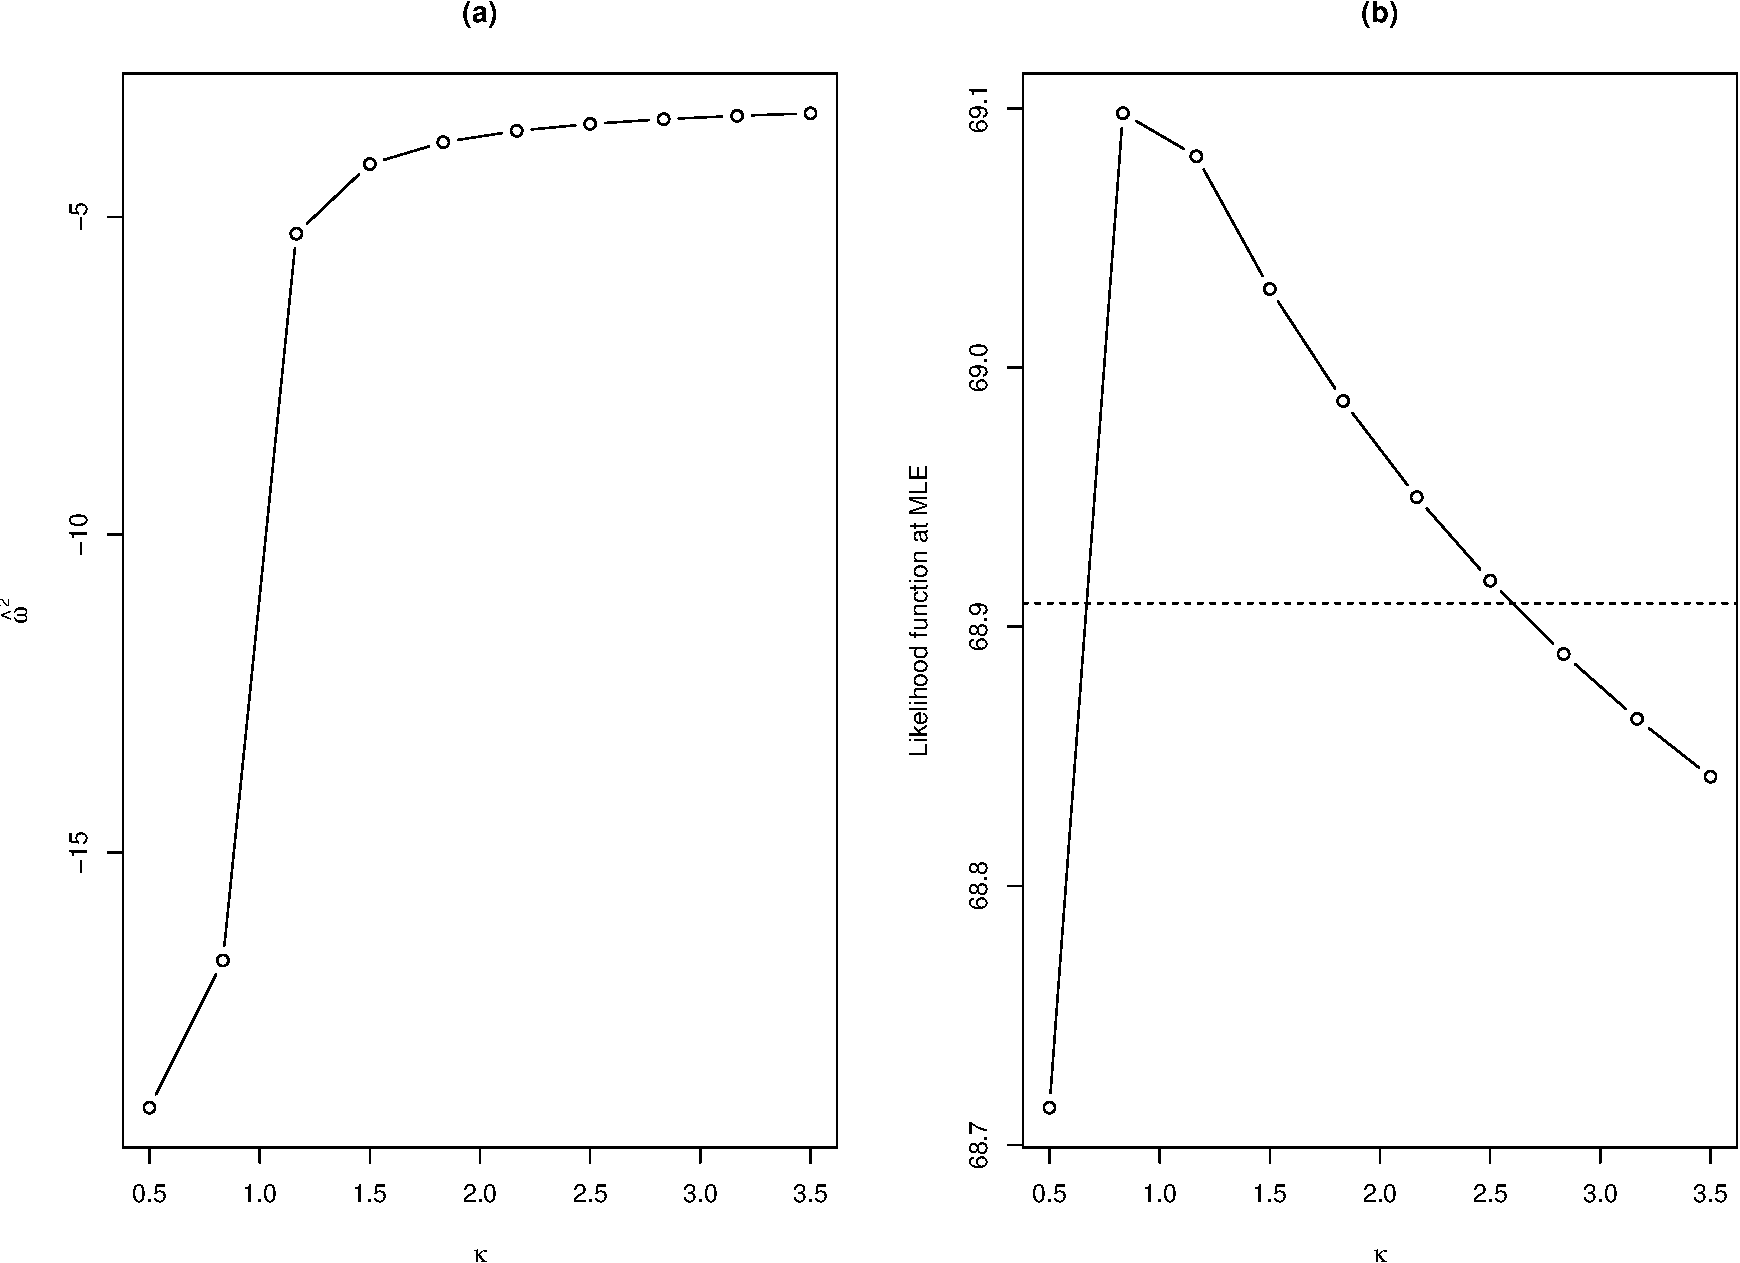
\includegraphics[width=8.5in,height=\textheight,keepaspectratio]{03_model-fitting_files/figure-pdf/fig-galicia-matern-1.pdf}

}

\caption{\label{fig-galicia-matern}(a) plot of the maximum likelihood
estimate for the variance of the measurement error \(U_i\), denoted in
the text as \(\omega^2\), against the chosen fixed value for \(\kappa\);
(b) profile likeihood for \(\kappa\) with the horizontal dashed line
corresponding to the (approximate) threshold for constructing a 95\%
confidence interval based on a \(\chi^2\) with one degree of freedom.}

\end{figure}%

By examining the results shown in panel (a) of
Figure~\ref{fig-galicia-matern}, we observe that, as expected, smaller
values for \(\kappa\) leads to smaller point estimates for \(\omega^2\)
and viceversa. This begs the question, what should be our chosen value
for \(\kappa\)?

To answer this question, a natural approach is to estimate the model for
different values of \(\kappa\) and see which one give the best fit to
the data, according to the likelihood function. In panel (b) of
Figure~\ref{fig-galicia-matern}, we show the results of this approach
where we considered 10 values for \(\kappa\) within the range 0.5 to 3.5
(see code above). In this plot, we have also added a horizontal line to
help us to approximate a range of the most plausible value for
\(\kappa\). More precisely, the horizontal dashed line is computed by
taking the maximum observed values of the likelihoods computed for the
different values of \(\kappa\), say \(\hat{M}\) and we subtract the
quantile 0.95 of a \(\chi^2\) distribution with 1 degree of freedom. In
R this horizontal line is obtained as

\begin{Shaded}
\begin{Highlighting}[]
\FunctionTok{max}\NormalTok{(llik\_values)}\SpecialCharTok{{-}}\FunctionTok{pchisq}\NormalTok{(}\FloatTok{0.95}\NormalTok{, }\AttributeTok{df =} \DecValTok{2}\NormalTok{)}\SpecialCharTok{/}\DecValTok{2}
\end{Highlighting}
\end{Shaded}

where \texttt{llik\_values} is as defined in the previous chunk of code.
Note that this approach is essentially constructing the profile
likelihood for \(\kappa\) which one could use to derive a confidence
interval for \(\kappa\) with a finer segmentation for
\texttt{kappa\_values}. However, our current objective is not to derive
the confidence interval for \(\kappa\), but rather to gain a broad
understanding of the \(\kappa\) values supported by the dataset. The
values of \(\kappa\) that corresponds to likelihood values above the
horizontal line are approximately between 0.75 and 2.75. Hence,
selecting \(\kappa=1.5\) seems to be a reasonable one in this case. Now,
you may be pondering: are there value other than \(\kappa=1.5\) that
could fit the data even better? Our answer is that it is not worth the
effort to try estimate \(\kappa\) more precisely because it is
empirically very difficult and, under some scenarios, even impossible.
Estimating \(\kappa\) poses a well-documented challenge in geostatistics
(Zhang (2004)), which justifies our adoption of a pragmatic approach
that sets it at a predefined value. This issue is also further
exacerbated when analyzing count data, which tend to be less informative
about the correlation structure than continuously measured data.

\subsection{\texorpdfstring{Modelling hierarchical geostatistical data
using the \texttt{re()}
function}{Modelling hierarchical geostatistical data using the re() function}}\label{sec-add-re-glgm}

We now consider the analysis of geostatistical data with a hierarchical
structure and show how to formulate and fit a geostatistical model that
accounts for the effects of the different layers of the data. For this
purpose, we use the \texttt{italy\_sim} where each of the sampled
locations can be grouped according to two administrative subdivisions of
Italy, regions (Admin level 2) and provinces (Admin level 3), as shown
in Figure~\ref{fig-italy-maps}.

\begin{Shaded}
\begin{Highlighting}[]
\FunctionTok{library}\NormalTok{(rgeoboundaries)}
\FunctionTok{library}\NormalTok{(mapview)}
\NormalTok{italy\_regions }\OtherTok{\textless{}{-}} \FunctionTok{geoboundaries}\NormalTok{(}\AttributeTok{country =} \StringTok{"italy"}\NormalTok{, }\AttributeTok{adm\_lvl =} \StringTok{"adm2"}\NormalTok{)}

\NormalTok{italy\_provinces }\OtherTok{\textless{}{-}} \FunctionTok{geoboundaries}\NormalTok{(}\AttributeTok{country =} \StringTok{"italy"}\NormalTok{, }\AttributeTok{adm\_lvl =} \StringTok{"adm3"}\NormalTok{)}
\end{Highlighting}
\end{Shaded}

\begin{Shaded}
\begin{Highlighting}[]
\FunctionTok{par}\NormalTok{(}\AttributeTok{mfrow =} \FunctionTok{c}\NormalTok{(}\DecValTok{1}\NormalTok{,}\DecValTok{2}\NormalTok{))}

\CommentTok{\# Map of the data with the region boundaries}
\NormalTok{map\_regions }\OtherTok{\textless{}{-}} \FunctionTok{ggplot}\NormalTok{() }\SpecialCharTok{+} 
\FunctionTok{geom\_sf}\NormalTok{(}\AttributeTok{data =}\NormalTok{ italy\_sim\_sf, }\AttributeTok{pch =} \DecValTok{4}\NormalTok{, }\AttributeTok{color =} \StringTok{"red"}\NormalTok{) }\SpecialCharTok{+} 
\FunctionTok{geom\_sf}\NormalTok{(}\AttributeTok{data =}\NormalTok{ italy\_regions, }\AttributeTok{fill =} \ConstantTok{NA}\NormalTok{) }\SpecialCharTok{+} 
\FunctionTok{theme\_void}\NormalTok{() }\SpecialCharTok{+}
\FunctionTok{labs}\NormalTok{(}\AttributeTok{title =} \StringTok{"Regions"}\NormalTok{) }\SpecialCharTok{+}
\FunctionTok{theme}\NormalTok{(}\AttributeTok{plot.title =} \FunctionTok{element\_text}\NormalTok{(}\AttributeTok{hjust =} \DecValTok{1}\SpecialCharTok{/}\DecValTok{2}\NormalTok{))}

\CommentTok{\# Map of the data with the province boundaries}
\NormalTok{map\_provinces }\OtherTok{\textless{}{-}} \FunctionTok{ggplot}\NormalTok{() }\SpecialCharTok{+} 
\FunctionTok{geom\_sf}\NormalTok{(}\AttributeTok{data =}\NormalTok{ italy\_sim\_sf, }\AttributeTok{pch =} \DecValTok{4}\NormalTok{, }\AttributeTok{color =} \StringTok{"red"}\NormalTok{) }\SpecialCharTok{+} 
\FunctionTok{geom\_sf}\NormalTok{(}\AttributeTok{data =}\NormalTok{ italy\_provinces, }\AttributeTok{fill =} \ConstantTok{NA}\NormalTok{) }\SpecialCharTok{+} 
\FunctionTok{theme\_void}\NormalTok{() }\SpecialCharTok{+}
\FunctionTok{labs}\NormalTok{(}\AttributeTok{title =} \StringTok{"Provinces"}\NormalTok{) }\SpecialCharTok{+}
\FunctionTok{theme}\NormalTok{(}\AttributeTok{plot.title =} \FunctionTok{element\_text}\NormalTok{(}\AttributeTok{hjust =} \DecValTok{1}\SpecialCharTok{/}\DecValTok{2}\NormalTok{))}

\FunctionTok{library}\NormalTok{(gridExtra)}
\FunctionTok{grid.arrange}\NormalTok{(map\_regions, map\_provinces, }\AttributeTok{ncol =} \DecValTok{2}\NormalTok{)}
\end{Highlighting}
\end{Shaded}

\begin{figure}[H]

\centering{

\pandocbounded{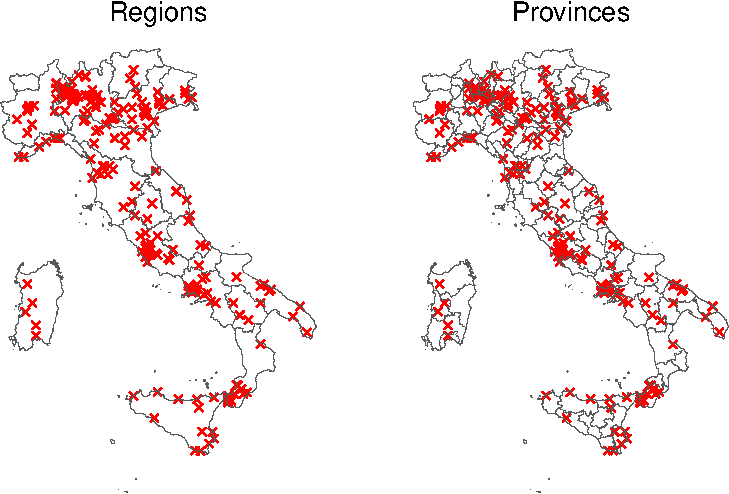
\includegraphics[keepaspectratio]{03_model-fitting_files/figure-pdf/fig-italy-maps-1.pdf}}

}

\caption{\label{fig-italy-maps}The plot shows the location of the
data-set \texttt{italy\_sim} (red crosses), with the boundaries of the
regions (left) and provinces (right) of Italy.}

\end{figure}%

Let \(V_h\), for \(h=1,\ldots,n_V\) and \(Z_k\), for
\(k=1,\ldots,n_{Z}\), be a set of mutually independent Gaussian
variables with zero means and variances \(\sigma^2_{V}\) and
\(\sigma^2_{Z}\), respectively. Finally let \(\mathcal{A}_h\), for
\(h=1,\ldots,n_V\) and \(\mathcal{B}_k\), for \(k=1,\ldots,n_{Z}\),
denote the areas encompassed by the boundaries of the region and
provinces, respectively. Since we have 10 repeated observations at each
locations, we shall use \(Y_{ij}\) to denote the \(j\)-th outcome (found
in the data under the column \texttt{y}) at the \(i\)-th location
\(x_i\). The model from which we generated data \(y_{ij}\) is
\begin{equation}\phantomsection\label{eq-italy-sim-model}{
Y_{ij} = \beta_0 + \overbrace{\beta_1 d(x_i) + S(x_i)}^\text{Location-level effect} + \underbrace{\sum_{h=1}^{n_{V}} I(x_i \in \mathcal{A}_h) \times V_h}_\text{Region effect} +\\ \overbrace{\sum_{k=1}^{n_{Z}} I(x_i \in \mathcal{B}_k) \times Z_k}^\text{Province effect} +  \underbrace{U_{ij}}_\text{Measurement error},
}\end{equation} for \(j=1,\ldots 10\) and \(i=1,\ldots,200\), where,
\(d(x_i)\) is the log-transformed population density,
\(I(x \in \mathcal{R})\) is an indicator function that takes value 1 if
the location \(x\) falls within the boundaries of the area denoted by
\(\mathcal{R}\) and 0 otherwise. The covariance function chosen in the
generation of the data was an exponential correlation function hence
\({\rm cov}\{S(x), S(x') = \sigma^2 \exp\{-||x-x'||/\phi\}\).

The inclusion of the random effects \(V_h\), for the region, and
\(Z_k\), for the province, can be included by using the \texttt{re()}
function into the \texttt{formula} passed to \texttt{glgpm} as shown
below.

\begin{Shaded}
\begin{Highlighting}[]

                        \CommentTok{\# Location{-}level effect}
\NormalTok{italy\_fit }\OtherTok{\textless{}{-}} \FunctionTok{glgpm}\NormalTok{( y }\SpecialCharTok{\textasciitilde{}} \FunctionTok{log}\NormalTok{(pop\_dens) }\SpecialCharTok{+} \FunctionTok{gp}\NormalTok{(}\AttributeTok{kappa =} \FloatTok{0.5}\NormalTok{, }\AttributeTok{nugget =} \DecValTok{0}\NormalTok{) }\SpecialCharTok{+}
                        \CommentTok{\# Region and province effects}
                        \FunctionTok{re}\NormalTok{(region, province),}
         \AttributeTok{data =}\NormalTok{ italy\_sim\_sf, }\AttributeTok{scale\_to\_km =} \ConstantTok{TRUE}\NormalTok{,}
         \AttributeTok{family =} \StringTok{"gaussian"}\NormalTok{)}
\DocumentationTok{\#\#   0:     441.00731: {-}0.404481  1.33798  0.00000  4.62406  0.00000  0.00000  0.00000}
\DocumentationTok{\#\#   1:    {-}130.05497: {-}0.408825  1.35003 {-}0.0387110  4.66059 {-}0.910409 {-}0.00265292 0.0107965}
\DocumentationTok{\#\#   2:    {-}268.13436: {-}0.865126  1.39525 {-}0.0305269  5.92133 {-}1.96079 {-}0.666581 0.487537}
\DocumentationTok{\#\#   3:    {-}329.24560: {-}1.44091  1.38139 {-}0.546306  4.98616 {-}1.67936 {-}1.15202 0.383821}
\DocumentationTok{\#\#   4:    {-}331.20861: {-}1.38498  1.37256 0.165463  5.61366 {-}1.63033 {-}2.11435 0.371263}
\DocumentationTok{\#\#   5:    {-}331.28418: {-}0.874796  1.37322 {-}0.271990  5.18071 {-}1.62887 {-}0.970704 0.371407}
\DocumentationTok{\#\#   6:    {-}331.42968: {-}1.04087  1.37294 {-}0.119652  5.33634 {-}1.62883 {-}1.33321 0.375031}
\DocumentationTok{\#\#   7:    {-}331.43375: {-}1.07312  1.37288 {-}0.0878211  5.36725 {-}1.62883 {-}1.42011 0.376251}
\DocumentationTok{\#\#   8:    {-}331.43375: {-}1.07445  1.37288 {-}0.0866254  5.36840 {-}1.62883 {-}1.42489 0.376323}
\DocumentationTok{\#\#   9:    {-}331.43375: {-}1.07445  1.37288 {-}0.0866254  5.36840 {-}1.62883 {-}1.42489 0.376323}

\FunctionTok{summary}\NormalTok{(italy\_fit)}
\DocumentationTok{\#\# Call:}
\DocumentationTok{\#\# glgpm(formula = y \textasciitilde{} log(pop\_dens) + gp(kappa = 0.5, nugget = 0) + }
\DocumentationTok{\#\#     re(region, province), data = italy\_sim\_sf, family = "gaussian", }
\DocumentationTok{\#\#     scale\_to\_km = TRUE)}
\DocumentationTok{\#\# }
\DocumentationTok{\#\# Linear geostatistical model}
\DocumentationTok{\#\# Link: identity }
\DocumentationTok{\#\# Inverse link function = x }
\DocumentationTok{\#\#  }
\DocumentationTok{\#\# \textquotesingle{}Lower limit\textquotesingle{} and \textquotesingle{}Upper limit\textquotesingle{} are the limits of the 95\% confidence level intervals}
\DocumentationTok{\#\# }
\DocumentationTok{\#\# Regression coefficients}
\DocumentationTok{\#\#                Estimate Lower limit Upper limit    StdErr z.value p.value    }
\DocumentationTok{\#\# (Intercept)   {-}1.074451   {-}2.031690   {-}0.117212  0.488396    {-}2.2 0.02781 *  }
\DocumentationTok{\#\# log(pop\_dens)  1.372877    1.352018    1.393735  0.010642   129.0 \textless{} 2e{-}16 ***}
\DocumentationTok{\#\# {-}{-}{-}}
\DocumentationTok{\#\# Signif. codes:  0 \textquotesingle{}***\textquotesingle{} 0.001 \textquotesingle{}**\textquotesingle{} 0.01 \textquotesingle{}*\textquotesingle{} 0.05 \textquotesingle{}.\textquotesingle{} 0.1 \textquotesingle{} \textquotesingle{} 1}
\DocumentationTok{\#\# }
\DocumentationTok{\#\#                         Estimate Lower limit Upper limit}
\DocumentationTok{\#\# Measuremment error var.   1.2167      1.2009      1.2327}
\DocumentationTok{\#\# }
\DocumentationTok{\#\# Spatial Gaussian process}
\DocumentationTok{\#\# Matern covariance parameters (kappa=0.5)}
\DocumentationTok{\#\#                       Estimate Lower limit Upper limit}
\DocumentationTok{\#\# Spatial process var.   0.91702     0.59470       1.414}
\DocumentationTok{\#\# Spatial corr. scale  214.51980   153.60751     299.587}
\DocumentationTok{\#\# Variance of the nugget effect fixed at 0}
\DocumentationTok{\#\# }
\DocumentationTok{\#\# Unstructured random effects}
\DocumentationTok{\#\#                             Estimate Lower limit Upper limit}
\DocumentationTok{\#\# region (random eff. var.)    0.24053     0.14553      0.3976}
\DocumentationTok{\#\# province (random eff. var.)  0.37632     0.35607      0.3977}
\DocumentationTok{\#\# }
\DocumentationTok{\#\# Log{-}likelihood: 331.4338}
\DocumentationTok{\#\# AIC: {-}648.8675}
\end{Highlighting}
\end{Shaded}

In the code above, the \texttt{factor} variables \texttt{region} and
\texttt{province} found in \texttt{italy\_sim} are passed to
\texttt{re()} and these are estimated as unstructured random effects as
defined by Equation~\ref{eq-italy-sim-model}. From the summary of model,
we then obtain the parameter and interval estimates as reported in
Table~\ref{tbl-italy-sim-mle}.

\begin{longtable}[]{@{}llll@{}}
\caption{Maximum likelihood estimates and, lower and upper limits of the
95\% confidence interval for the parameters of the model in
Equation~\ref{eq-italy-sim-lmm}.}\label{tbl-italy-sim-mle}\tabularnewline
\toprule\noalign{}
Parameter & Point estimate & Lower limit & Upper limit \\
\midrule\noalign{}
\endfirsthead
\toprule\noalign{}
Parameter & Point estimate & Lower limit & Upper limit \\
\midrule\noalign{}
\endhead
\bottomrule\noalign{}
\endlastfoot
\(\beta_0\) & -1.074 & -2.032 & -0.117 \\
\(\beta_1\) & 1.373 & 1.352 & 1.394 \\
\(\sigma^2\) & 0.917 & 0.595 & 1.414 \\
\(\phi\) & 214.520 & 153.608 & 299.587 \\
\(\sigma^2_{V}\) & 0.241 & 0.146 & 0.398 \\
\(\sigma^2_{Z}\) & 1.457 & 1.379 & 1.540 \\
\(\omega^2\) & 0.196 & 0.194 & 0.199 \\
\end{longtable}

The function \texttt{to\_table} from the \texttt{RiskMap} package can be
used to obtain the Latex or HTML code directly from a fit of the model.
Here is an example.

\begin{Shaded}
\begin{Highlighting}[]
\FunctionTok{to\_table}\NormalTok{(italy\_fit, }\AttributeTok{digits =} \DecValTok{3}\NormalTok{)}
\DocumentationTok{\#\# \% latex table generated in R 4.5.1 by xtable 1.8{-}4 package}
\DocumentationTok{\#\# \% Mon Sep 29 22:19:40 2025}
\DocumentationTok{\#\# \textbackslash{}begin\{table\}[ht]}
\DocumentationTok{\#\# \textbackslash{}centering}
\DocumentationTok{\#\# \textbackslash{}begin\{tabular\}\{rrrr\}}
\DocumentationTok{\#\#   \textbackslash{}hline}
\DocumentationTok{\#\#  \& Estimate \& Lower limit \& Upper limit \textbackslash{}\textbackslash{} }
\DocumentationTok{\#\#   \textbackslash{}hline}
\DocumentationTok{\#\# (Intercept) \& {-}1.074 \& {-}2.032 \& {-}0.117 \textbackslash{}\textbackslash{} }
\DocumentationTok{\#\#   log(pop\textbackslash{}\_dens) \& 1.373 \& 1.352 \& 1.394 \textbackslash{}\textbackslash{} }
\DocumentationTok{\#\#   Spatial process var. \& 0.917 \& 0.595 \& 1.414 \textbackslash{}\textbackslash{} }
\DocumentationTok{\#\#   Spatial corr. scale \& 214.520 \& 153.608 \& 299.587 \textbackslash{}\textbackslash{} }
\DocumentationTok{\#\#   region (random eff. var.) \& 0.241 \& 0.146 \& 0.398 \textbackslash{}\textbackslash{} }
\DocumentationTok{\#\#   province (random eff. var.) \& 0.376 \& 0.356 \& 0.398 \textbackslash{}\textbackslash{} }
\DocumentationTok{\#\#   Measuremment error var. \& 1.217 \& 1.201 \& 1.233 \textbackslash{}\textbackslash{} }
\DocumentationTok{\#\#    \textbackslash{}hline}
\DocumentationTok{\#\# \textbackslash{}end\{tabular\}}
\DocumentationTok{\#\# \textbackslash{}end\{table\}}
\end{Highlighting}
\end{Shaded}

\section{Generalized linear geostatistical
models}\label{generalized-linear-geostatistical-models}

We now consider the modelling of count outcomes, focusing our attention
to the Binomial and Poisson geostatistical models.

The use of Binomial geostatistical model is appropriate whenever the
reported counts have a known upper bound. For example, when analyzing
aggregated disease counts from cross-sectional survey data, the total
number of people sampled at a location defines the largest number of
possible reported disease cases. Recalling the model specification of
Table~\ref{tbl-glm}, we specify the Binomial geostatistical model by
stating that the reported disease counts \(Y_i\) out of \(n_i\) (the
maximum value that \(Y_i\) can take) at location \(x_i\), conditionally
on the spatial random effects \(S(x_i)\), follow a Binomial distribution
with probability \(p(x_i)\) and logit-linear predictor
\begin{equation}\phantomsection\label{eq-lp-bin}{
\log\left\{\frac{p(x_i)}{1-p(x_i)}\right\} = d(x_i)^\top \beta + S(x_i).
}\end{equation} In this model, \(p(x_i)\) is commonly understood as
representing the prevalence of the disease under consideration, defined
as the proportion of individuals with the disease at a specific moment.
While \(p(x_i)\) is not strictly a proportion, its interpretation as
disease prevalence is justified by the fact that if we were to sample a
sufficiently large population at location \(x_i\), the proportion of
individuals with the disease would converge closely to the value of
\(p(x_i)\).

A Binomial geostatistical model is also used when analyzing data at
individual level where the outcome is binary and usually indicates the
positive or negative result of a test for a disease under investigation.
In this analysis, a mix of individual-level variables and location-level
variables could be introduced to model the probability of a positive
test. To formally write the model, we now use \(Y_{ij}\) to indicate the
binary outcome taking value 1, if the test was positive, and 0, if
negative, for the \(j\)-th individual sampled at location \(x_i\). The
linear predictor now takes the form
\begin{equation}\phantomsection\label{eq-lp-bin-ind}{
\log\left\{\frac{p_{ij}}{1-p_{ij}}\right\} = e_{ij}^\top \gamma + d(x_{i})^\top \beta + S(x_i).
}\end{equation} In the model above we have distinguished between
covariates \(e_{ij}\), that express the effect on \(p_{ij}\) due to
individual traits (such as age and gender), and covariates \(d(x_i)\),
that instead quantify the effect on \(p_{ij}\) resulting from the
environmental attributes of location \(x_i\) (such as elevation,
temperature, and precipitation). In this model \(p_{ij}\) -- the
probability of a positive test -- once again can be interpreted as the
disease prevalence for a population characterized by the individual
traits \(e_{ij}\) and residing at location \(x_i\).

Finally, when the counts arise from a population whose size is unknown
or when the occurrence of a disease is very small relative to the size
of the target population, one should consider the use of a Poisson
geostaistical model. We then use \(Y_i\) to denote the reported counts
at location \(x_i\) and assume that this, conditionally on a Gaussian
process \(S(x_i)\), follows a Poisson distribution with mean
\(\lambda(x_i)\) and log-linear predictor
\begin{equation}\phantomsection\label{eq-poisson-lp}{
\log\left\{\lambda(x_i)\right\} = d(x_i)^\top \beta + S(x_i). 
}\end{equation} If for example, \(Y_i\) corresponds to the number of new
cases reported at a health facility at location \(x_i\) over a certain,
the \(\lambda(x_i)\) is interpreted as the average number of new cases
reported over that period. If the information on the size of the
population at risk for the diseases were available, this can be
incorporated into the model so as to enable the interpretation of
\(\lambda(x_i)\) as the disease incidence, defined as the total number
of new cases reported over a given period of time divided by the
population at risk. If we denote the latter as \(m_i\), then we would
specify the mean of \(Y_i\) as \(m_i\lambda(x_i)\) an model
\(\lambda(x_i)\) as already specified in Equation~\ref{eq-poisson-lp}.
Another prevalent application of the Poisson geostatistical model in
epidemiology involves mapping the abundance of disease vectors. Here,
\(\lambda(x_i)\) corresponds to the mean number of vectors per unit
area. Also, note that in this last scenario \(m_i\) cannot be defined as
it is the goal of the analysis to infer the vector population size at
location \(x_i\).

In all the three models, namely Equation~\ref{eq-lp-bin},
Equation~\ref{eq-lp-bin-ind} and Equation~\ref{eq-poisson-lp}, one might
consider the inclusion of an additional random effect \(Z_i\),
previously used for the linear geostatistical model, to account for
small spatial variation or overdispersion that stems from the omission
of covariates that may not necessarily exhibit spatial structure, such
as behavioral or genetic traits. We shall further elaborate and provide
guidance on this point in the following examples of this section.

\subsection{Example: river-blindness in
Liberia}\label{sec-liberia-estim1}

In section Section~\ref{sec-agg-count-exp}, we carried out the
exploratory analysis of the river-blindness prevalence data to assess
how the covariate of elevation could be introduced into the model. In
Section~\ref{sec-empirical-variog-bin}, we then tested for residual
spatial correlation, when the log-transformed elevation is used as a
covariate, using the empirical variogram. Based on these results, we now
formulate a fit a Binomial geostatistical model to data. To achieve
this, we extend the model presented in
Equation~\ref{eq-liberia-bin-mixed-elev} through the inclusion of a
spatial Gaussian process, \(S(x)\), hence we write
\begin{equation}\phantomsection\label{eq-liberia-geostat-bin-elev}{
\log\left\{\frac{p(x_i)}{1-p(x_i)}\right\} = \beta_{0} + \beta_{1}\log\{e(x_i)\} + S(x_i) + Z_i.
}\end{equation} We shall assume that \(S(x_i)\) is a stationary
isotropic Gaussian process with an exponential correlation function
function \(\rho(u) = \exp\{-u/\phi\}\), with scale parameter \(\phi\).

We apply the Monte Carlo Maximum Likelihood (MCML) method for parameter
estimation, which is implemented via the \texttt{glgpm} function. In
this section, we set aside the technical details of the estimation
process to focus exclusively on interpreting the results. A more
detailed explanation of the MCML theory can be found in
Section~\ref{sec-glgm-lik}, with a concise summary of the practical
aspects provided in Section~\ref{sec-summary}.

\begin{Shaded}
\begin{Highlighting}[]
\NormalTok{fit\_liberia }\OtherTok{\textless{}{-}} 
  \FunctionTok{glgpm}\NormalTok{(npos }\SpecialCharTok{\textasciitilde{}} \FunctionTok{log}\NormalTok{(elevation) }\SpecialCharTok{+} \FunctionTok{gp}\NormalTok{(long, lat),}
        \AttributeTok{den =}\NormalTok{ ntest, }\AttributeTok{data =}\NormalTok{ liberia,}
        \AttributeTok{crs =} \DecValTok{4326}\NormalTok{,}
        \AttributeTok{convert\_to\_crs =} \DecValTok{32629}\NormalTok{,}
        \AttributeTok{family =} \StringTok{"binomial"}\NormalTok{)}
\end{Highlighting}
\end{Shaded}

\begin{verbatim}
  0:    -0.0000000: -2.99847 0.313076  0.00000  4.21726
  1:   -0.80648178: -3.00931 0.276022 -0.0591718  4.25297
  2:    -3.6370983: -3.01220 0.289555 -0.121723  4.29346
  3:    -8.9791361: -3.02029 0.292164 -0.612427  4.65656
  4:    -10.138726: -3.01403 0.321979 -0.618511  4.66123
  5:    -10.460755: -3.01539 0.315916 -0.618614  4.66104
  6:    -10.708401: -3.01730 0.303633 -0.619068  4.66108
  7:    -10.867171: -3.01778 0.307844 -0.629820  4.65512
  8:    -13.011075: -3.03426 0.311082 -1.74183  3.40939
  9:    -13.747654: -3.05019 0.314551 -1.55765  3.47010
 10:    -13.761926: -3.05667 0.315882 -1.52417  3.49985
 11:    -13.761964: -3.05673 0.315896 -1.52242  3.50235
 12:    -13.761964: -3.05673 0.315896 -1.52242  3.50236
\end{verbatim}

\begin{Shaded}
\begin{Highlighting}[]
\FunctionTok{summary}\NormalTok{(fit\_liberia)}
\end{Highlighting}
\end{Shaded}

\begin{verbatim}
Call:
glgpm(formula = npos ~ log(elevation) + gp(long, lat), data = liberia, 
    family = "binomial", den = ntest, crs = 4326, convert_to_crs = 32629)

Binomial geostatistical linear model
Link: canonical 
Inverse link function = stats::plogis(x) 
 
'Lower limit' and 'Upper limit' are the limits of the 95% confidence level intervals

Regression coefficients
                Estimate Lower limit Upper limit    StdErr z.value   p.value
(Intercept)    -3.056728   -3.594341   -2.519115  0.274297 -11.144 < 2.2e-16
log(elevation)  0.315896    0.260811    0.370981  0.028105  11.240 < 2.2e-16
                  
(Intercept)    ***
log(elevation) ***
---
Signif. codes:  0 '***' 0.001 '**' 0.01 '*' 0.05 '.' 0.1 ' ' 1

Spatial Gaussian process
Matern covariance parameters (kappa=0.5)
                     Estimate Lower limit Upper limit
Spatial process var.  0.21818     0.18964       0.251
Spatial corr. scale  33.19362    28.30045      38.933
Variance of the nugget effect fixed at 0

Log-likelihood: 13.76196
\end{verbatim}

When using the \texttt{glgpm} function to fit a Binomial model, we need
to specify the Binomial denominators, i.e.~the number of tested at a
location in this case, through the argument \texttt{den}. Other
arguments of \texttt{glgpm} that are used for carrying out MCML are
\texttt{control\_mcmc}, that defines the setting parameters of the Monte
Carlo Markov Chain algorithm, and \texttt{par0}, which represents our
best guess for the unknown parameters of the Binomial geostatistical
model. For more information on how the default values of these two
arguments, we refer the reader the to the help page of the
\texttt{glgpm} function. To understand how to change the default
parameters in order to improve the MCML estimation, we advise you to
read Section~\ref{sec-mcml}. Also, remember that to enable the
estimation of the nugget effect, \(Z_i\), you should set
\texttt{nugget=NULL} in the \texttt{gp} function, since by default the
\texttt{glgpm} function excludes \(Z_i\) when the out is non-Gaussian.

In the above summary of the model, the interpretation of the regression
coefficients is the same as in a standard logistic regression model.
Hence, by taking the exponential of the estimate for the regression
coefficient \(\beta_1\), we could then express the effect for a unit
increase in the covariate -- in this case the log-transformed elevation
-- on the odds of disease prevalence. Finally, the interpretation of
estimates of the covariance parameters is not affected by the type of
distribution used to model the main outcome. From the above summary, we
note the larger estimates of \(\sigma^2\) than \(\tau^2\) which suggest
the dominance of spatial variation over the unstructured variation in
the unexplained variation of disease prevalence. Finally, the estimate
of \(\phi\) indicates a relatively large spatial correlation with a
\emph{practical range} close to (\(58.67 \times 3 \approx\))180km.

\subsection{\texorpdfstring{Example: \emph{Anopheles Gambiae} mosquitoes
in
Cameroon}{Example: Anopheles Gambiae mosquitoes in Cameroon}}\label{sec-anopheles-fit}

In Section~\ref{sec-agg-count-exp}, we explored the association between
elevation and the number of mosquitoes and found that the data showed
that on average, the number of ``Anopheles Gambiae* (A. Gambiae)
decreases for increasing elevation. We now fit a log-linear Poisson
geostatistical model, with linear predictor
\begin{equation}\phantomsection\label{eq-anopheles}{
\lambda(x_i) = \beta_0 + \beta_1 d(x_i) + S(x_i)
}\end{equation} where \(d(x_i)\) correspond to the elevation in meters
at location \(x_i\). This time, we first convert the data frame
\texttt{anopheles} into an \texttt{sf} object. This step is optional but
recommended as it allows us to simply the code syntax.

\begin{Shaded}
\begin{Highlighting}[]
\NormalTok{anopheles }\OtherTok{\textless{}{-}} \FunctionTok{st\_as\_sf}\NormalTok{(anopheles, }\AttributeTok{coords =} \FunctionTok{c}\NormalTok{(}\StringTok{"web\_x"}\NormalTok{, }\StringTok{"web\_y"}\NormalTok{),}
                      \AttributeTok{crs =} \DecValTok{3857}\NormalTok{)}
\end{Highlighting}
\end{Shaded}

We can then use the following script to fit the model in
\texttt{RiskMap}.

\begin{Shaded}
\begin{Highlighting}[]
\FunctionTok{set.seed}\NormalTok{(}\DecValTok{1}\NormalTok{)}
\NormalTok{an\_fit }\OtherTok{\textless{}{-}} 
\FunctionTok{glgpm}\NormalTok{(An.gambiae }\SpecialCharTok{\textasciitilde{}}\NormalTok{ elevation }\SpecialCharTok{+} \FunctionTok{gp}\NormalTok{(),}
      \AttributeTok{data =}\NormalTok{ anopheles, }
      \AttributeTok{family =} \StringTok{"poisson"}\NormalTok{, }\AttributeTok{messages =} \ConstantTok{FALSE}\NormalTok{)}

\FunctionTok{summary}\NormalTok{(an\_fit)}
\end{Highlighting}
\end{Shaded}

\begin{verbatim}
Call:
glgpm(formula = An.gambiae ~ elevation + gp(), data = anopheles, 
    family = "poisson", messages = FALSE)

Poisson geostatistical linear model
Link: canonical 
Inverse link function = exp(x) 
 
'Lower limit' and 'Upper limit' are the limits of the 95% confidence level intervals

Regression coefficients
               Estimate Lower limit Upper limit      StdErr z.value   p.value
(Intercept)  3.69384399  3.00784989  4.37983809  0.35000342  10.554 < 2.2e-16
elevation   -0.00283997 -0.00336073 -0.00231922  0.00026569 -10.689 < 2.2e-16
               
(Intercept) ***
elevation   ***
---
Signif. codes:  0 '***' 0.001 '**' 0.01 '*' 0.05 '.' 0.1 ' ' 1

Spatial Gaussian process
Matern covariance parameters (kappa=0.5)
                     Estimate Lower limit Upper limit
Spatial process var.  0.67165     0.59987      0.7520
Spatial corr. scale   4.38649     3.84756      5.0009
Variance of the nugget effect fixed at 0

Log-likelihood: 9.453628
\end{verbatim}

The estimate, \(\hat{\beta}_1\), for the regression coefficient
\(\beta_1\) suggests that for a 100 meters drop in elevation, the
average number of mosquitoes decreases by about
\((100\times\exp\{100\times -0.018\}\approx)17\%\). The order of
magnitude of the estimates suggest the presence of residual spatial
correlation, albeit on a rather small scale.

\begin{Shaded}
\begin{Highlighting}[]
\FunctionTok{dist\_summaries}\NormalTok{(anopheles, }\AttributeTok{scale\_to\_km =} \ConstantTok{TRUE}\NormalTok{)}
\end{Highlighting}
\end{Shaded}

\begin{verbatim}
$min
[1] 0.3828559

$max
[1] 160.388

$mean
[1] 54.58734

$median
[1] 43.70518
\end{verbatim}

Using the \texttt{dist\_summaries} function, we can see that the average
distance is about 55km and the minimum is about 387 meters. The estimate
of phi of 4km is thus relatively small compared to the the distances
between locations in the data. In Chapter~\ref{sec-geo-prediction}, we
will further investigate to what extent this small-scale spatial
correlation can affect the predictions of the An. Gambiae counts.

\subsection{Using parametric bootstrap for computing confidence
intervals}\label{sec-bootstrap}

The bootstrap is a widely used resampling technique introduced by Efron
(1979) as a general approach to estimating the variability of
statistical estimates without relying on strong parametric assumptions.
While the classical non-parametric bootstrap resamples directly from the
observed data, parametric bootstrap instead relies on simulating new
datasets from an assumed parametric model, using plug-in estimated
obtain from the original fit of the model to the data. This
simulation-based method is particularly useful for complex models, such
as those considered in this book, that yield an intractable likelihood
function.

We now describe how to carry out parametric bootstrap for geostatsitical
models in \texttt{RiskMap}. The use of simulation-based approaches will
be more extensively covered in Chapter~\ref{sec-geo-prediction}, but,
for the purpose of this section, it is first important to understand how
data can be simulated from a geostatistical model.

The way we have formulated geostatistical models in
Section~\ref{sec-geostat-models} provides a hint as to what step should
be followed when simulating from a geostatistical model. Using the same
notation of Section~\ref{sec-geostat-models}, these are the steps.

\begin{enumerate}
\def\labelenumi{\arabic{enumi}.}
\item
  For a given set of predefined locations \(X\) compute the covariance
  matrix \(\Sigma\) with \((i,j)\)-th entry \(\sigma^2 \rho(u_{ij})\).
\item
  Compute the covariate effects \(d(x)^\top \beta\) for all the
  locations in \(X\).
\item
  Simulate \(B\) times from a multivariate Gaussian distribution with
  mean vector 0 and covariance \(\Sigma\) as previously defined. We
  denote the output from this step as \(S_{(j)}(x)\), for
  \(j = 1, \ldots, B\).
\item
  Compute the linear predictor at each location of \(X\), by adding the
  covariate effects from step 2 to the simulated random effects from
  step 3, hence \(g\{\mu_{(j)}(x)\} = d(x)^\top \beta + S_{(j)}(x)\).
\end{enumerate}

Note that before performing the steps above, the values of the model
parameters must be fixed. For example, if simulating from a model fitted
to the data, the values of the model parameters should be the maximum
likelihood estimates. If the goal is to simulate actual observations for
the outcome \(Y\) at the locations \(X\), then we need to add the
following steps.

5A. If the nugget term is included in the model, draw samples
\(Z_{(j)}\) for each location in \(X\) from a Gaussian distribution with
mean 0 and variance \(\tau^2\). Add the simulated values \(Z_{(j)}\) to
\(g\{\mu_{(j)}(x)\}\).

6A. Compute \(\mu_{(j)}(x)\) by applying the inverse link function
\(g^{-1}(\cdot)\) to the samples of the linear predictor previously
computed.

7A. Simulate from the distribution of \(Y\) given \(\mu_{(j)}(x)\),
according to the chosen model, for \(j = 1, \ldots, B\).

These steps, from 1 to 7A, have been implemented in the
\texttt{glgpm\_sim} function. To show how to perform parametric
bootstrap in \texttt{RiskMap}, let us consider the Liberia data on
riverblindness and fit the following geostatistical model.

\begin{Shaded}
\begin{Highlighting}[]
\NormalTok{fit\_liberia\_no\_nugget }\OtherTok{\textless{}{-}} 
  \FunctionTok{glgpm}\NormalTok{(npos }\SpecialCharTok{\textasciitilde{}} \FunctionTok{log}\NormalTok{(elevation) }\SpecialCharTok{+} \FunctionTok{gp}\NormalTok{(long, lat),}
        \AttributeTok{den =}\NormalTok{ ntest, }\AttributeTok{data =}\NormalTok{ liberia,}
        \AttributeTok{crs =} \DecValTok{4326}\NormalTok{,}
        \AttributeTok{convert\_to\_crs =} \DecValTok{32629}\NormalTok{,}
        \AttributeTok{family =} \StringTok{"binomial"}\NormalTok{)}
\end{Highlighting}
\end{Shaded}

Using the fitted Binomial geostatistical above, we can simulate a single
dataset as follows:

\begin{Shaded}
\begin{Highlighting}[]
\NormalTok{liberia\_sim }\OtherTok{\textless{}{-}} \FunctionTok{glgpm\_sim}\NormalTok{(}\AttributeTok{n\_sim =} \DecValTok{1}\NormalTok{, }\AttributeTok{model\_fit =}\NormalTok{ fit\_liberia\_no\_nugget)}
\end{Highlighting}
\end{Shaded}

The output \texttt{liberia\_sim} is a list with as many components as
indicated by \texttt{n\_sim}. In this this case, we can access the
simulated data-set as \texttt{liberia\_sim{[}{[}1{]}{]}}. For example,
we could refit the same model to the simulated data as

\begin{Shaded}
\begin{Highlighting}[]
\NormalTok{fit\_liberia\_no\_nugget\_sim }\OtherTok{\textless{}{-}} 
\FunctionTok{glgpm}\NormalTok{(}\AttributeTok{formula =}\NormalTok{ npos }\SpecialCharTok{\textasciitilde{}} \FunctionTok{log}\NormalTok{(elevation) }\SpecialCharTok{+} \FunctionTok{gp}\NormalTok{(long, lat), }
    \AttributeTok{data =}\NormalTok{ liberia\_sim[[}\DecValTok{1}\NormalTok{]], }\AttributeTok{family =} \StringTok{"binomial"}\NormalTok{, }\AttributeTok{den =}\NormalTok{ ntest, }
    \AttributeTok{crs =} \DecValTok{32629}\NormalTok{)}
\end{Highlighting}
\end{Shaded}

Note that if the data's CRS has been converted, the simulated data-set
will inherit the new CRS rather than the original. This means that any
transformation applied to the CRS before simulation (e.g., from
geographic to projected coordinates) will affect the spatial scale and
interpretation of the simulated data.

This idea can be extended naturally to perform parametric bootstrap. The
procedure involves simulating multiple data-sets from the fitted model,
refitting the model to each of them, and extracting the estimates of
interest. For instance, the following code simulates 100 datasets and
fits the same model to each, storing the estimated regression
coefficients:

\begin{Shaded}
\begin{Highlighting}[]
\CommentTok{\# Simulate 100 datasets}
\NormalTok{n\_sim }\OtherTok{\textless{}{-}} \DecValTok{100}
\NormalTok{liberia\_boot }\OtherTok{\textless{}{-}} \FunctionTok{glgpm\_sim}\NormalTok{(}\AttributeTok{n\_sim =}\NormalTok{ n\_sim, }\AttributeTok{model\_fit =}\NormalTok{ fit\_liberia\_no\_nugget)}

\CommentTok{\# List where we will store the estimates from each of the simulated data{-}sets}
\NormalTok{par\_hat }\OtherTok{\textless{}{-}} \FunctionTok{list}\NormalTok{()}

\ControlFlowTok{for}\NormalTok{(i }\ControlFlowTok{in} \DecValTok{1}\SpecialCharTok{:}\NormalTok{n\_sim) \{}
  
  \CommentTok{\# Extracting the simulated Binomial data into "npos\_sim"}
\NormalTok{  liberia\_boot}\SpecialCharTok{$}\NormalTok{data\_sim}\SpecialCharTok{$}\NormalTok{npos\_sim }\OtherTok{\textless{}{-}}  
\NormalTok{    liberia\_boot}\SpecialCharTok{$}\NormalTok{data\_sim[[}\FunctionTok{paste}\NormalTok{(}\StringTok{"npos\_sim"}\NormalTok{,i,}\AttributeTok{sep=}\StringTok{""}\NormalTok{)]]}
  
  \CommentTok{\# Fitting the geostatistical model}
\NormalTok{  fit\_sim }\OtherTok{\textless{}{-}} \FunctionTok{glgpm}\NormalTok{(}
    \AttributeTok{formula =}\NormalTok{ npos\_sim }\SpecialCharTok{\textasciitilde{}} \FunctionTok{log}\NormalTok{(elevation) }\SpecialCharTok{+} \FunctionTok{gp}\NormalTok{(long, lat), }
    \AttributeTok{data =}\NormalTok{ liberia\_boot}\SpecialCharTok{$}\NormalTok{data\_sim, }
    \AttributeTok{family =} \StringTok{"binomial"}\NormalTok{, }
    \AttributeTok{par0 =} \FunctionTok{coef}\NormalTok{(fit\_liberia\_no\_nugget),}
    \AttributeTok{den =}\NormalTok{ ntest, }
    \AttributeTok{crs =} \DecValTok{32629}
\NormalTok{  ) }
  
  \CommentTok{\# Extracting the parameter estimates}
\NormalTok{  par\_hat[[i]] }\OtherTok{\textless{}{-}} \FunctionTok{coef}\NormalTok{(fit\_sim)}
  
\NormalTok{\}}
\end{Highlighting}
\end{Shaded}

After obtaining the parameter estimates, we extract them and rearrange
them in a matrix format to facilitate the computation of any summary,
including the confidence intervals as shown in the code below.

\begin{Shaded}
\begin{Highlighting}[]

\CommentTok{\# Extract all parameters maintaining beta as a vector}
\NormalTok{all\_params }\OtherTok{\textless{}{-}} \FunctionTok{sapply}\NormalTok{(}\DecValTok{1}\SpecialCharTok{:}\NormalTok{n\_sim, }\ControlFlowTok{function}\NormalTok{(i) \{}
   \FunctionTok{c}\NormalTok{(par\_hat[[i]]}\SpecialCharTok{$}\NormalTok{beta,  }
\NormalTok{     par\_hat[[i]]}\SpecialCharTok{$}\NormalTok{sigma2,}
\NormalTok{     par\_hat[[i]]}\SpecialCharTok{$}\NormalTok{phi)\})}


\NormalTok{CI }\OtherTok{\textless{}{-}} \FunctionTok{t}\NormalTok{(}\FunctionTok{apply}\NormalTok{(all\_params, }\DecValTok{1}\NormalTok{, }\ControlFlowTok{function}\NormalTok{(x) }\FunctionTok{quantile}\NormalTok{(x, }\FunctionTok{c}\NormalTok{(}\FloatTok{0.025}\NormalTok{, }\FloatTok{0.975}\NormalTok{))))}
\NormalTok{p }\OtherTok{\textless{}{-}} \DecValTok{2}
\FunctionTok{rownames}\NormalTok{(CI)[(p}\SpecialCharTok{+}\DecValTok{1}\NormalTok{)}\SpecialCharTok{:}\NormalTok{(p}\SpecialCharTok{+}\DecValTok{2}\NormalTok{)] }\OtherTok{\textless{}{-}} \FunctionTok{c}\NormalTok{(}\StringTok{"sigma\^{}2"}\NormalTok{, }\StringTok{"phi"}\NormalTok{)}

\FunctionTok{summary}\NormalTok{(fit\_liberia\_no\_nugget)}
\DocumentationTok{\#\# Call:}
\DocumentationTok{\#\# glgpm(formula = npos \textasciitilde{} log(elevation) + gp(long, lat), data = liberia, }
\DocumentationTok{\#\#     family = "binomial", den = ntest, crs = 4326, convert\_to\_crs = 32629)}
\DocumentationTok{\#\# }
\DocumentationTok{\#\# Binomial geostatistical linear model}
\DocumentationTok{\#\# Link: canonical (logit) }
\DocumentationTok{\#\# Inverse link function = 1 / (1 + exp({-}x)) }
\DocumentationTok{\#\#  }
\DocumentationTok{\#\# \textquotesingle{}Lower limit\textquotesingle{} and \textquotesingle{}Upper limit\textquotesingle{} are the limits of the 95\% confidence level intervals}
\DocumentationTok{\#\# }
\DocumentationTok{\#\# Regression coefficients}
\DocumentationTok{\#\#                 Estimate Lower limit Upper limit    StdErr z.value   p.value}
\DocumentationTok{\#\# (Intercept)    {-}2.847156   {-}3.272762   {-}2.421550  0.217150 {-}13.111 \textless{} 2.2e{-}16}
\DocumentationTok{\#\# log(elevation)  0.264436    0.222902    0.305970  0.021191  12.479 \textless{} 2.2e{-}16}
\DocumentationTok{\#\#                   }
\DocumentationTok{\#\# (Intercept)    ***}
\DocumentationTok{\#\# log(elevation) ***}
\DocumentationTok{\#\# {-}{-}{-}}
\DocumentationTok{\#\# Signif. codes:  0 \textquotesingle{}***\textquotesingle{} 0.001 \textquotesingle{}**\textquotesingle{} 0.01 \textquotesingle{}*\textquotesingle{} 0.05 \textquotesingle{}.\textquotesingle{} 0.1 \textquotesingle{} \textquotesingle{} 1}
\DocumentationTok{\#\# }
\DocumentationTok{\#\# Spatial Gaussian process}
\DocumentationTok{\#\# Matern covariance parameters (kappa=0.5)}
\DocumentationTok{\#\#                      Estimate Lower limit Upper limit}
\DocumentationTok{\#\# Spatial process var.  0.24447     0.21200      0.2819}
\DocumentationTok{\#\# Spatial corr. scale  34.04827    29.21324     39.6835}
\DocumentationTok{\#\# Variance of the nugget effect fixed at 0}
\DocumentationTok{\#\# }
\DocumentationTok{\#\# Log{-}likelihood: 13.75077}

\NormalTok{CI}
\DocumentationTok{\#\#                      2.5\%      97.5\%}
\DocumentationTok{\#\# (Intercept)    {-}3.6210256 {-}2.2028113}
\DocumentationTok{\#\# log(elevation)  0.1490998  0.4370221}
\DocumentationTok{\#\# sigma\^{}2         0.1134865  0.4085383}
\DocumentationTok{\#\# phi            14.3625701 80.5595429}
\end{Highlighting}
\end{Shaded}

By comparing the 95\(\%\) confidence intervals obtained from the
\texttt{summary} of the fitted model with those derived from the
bootstrap approach, we observe that the former are considerably narrower
for the covariance parameters, while the intervals are fairly similar
for the regression coefficients.

This discrepancy arises because the Wald-type confidence intervals from
\texttt{summary} rely on a Gaussian approximation of the maximum
likelihood estimator for the covariance parameters, which may not be
entirely reliable. (To improve the accuracy of this approximation,
\texttt{RiskMap} applies it to the log-transformed parameters and then
transforms the confidence intervals back to the original scale.) On the
other hand, bootstrap-based confidence intervals tend to be more
reliable, as they are not dependent on the Gaussian assumption. However,
they are also more computationally demanding. The use of only 100
bootstrap samples, as shown above, may indeed be insufficient. It is
generally recommended to use at least 1000 iterations, if
computationally feasible, to minimize the Monte Carlo error arising from
the bootstrap simulations.

\section{The residuals of a geostatistical model: issues to
consider}\label{the-residuals-of-a-geostatistical-model-issues-to-consider}

In geostatistical models, the concept of residuals, which are widely
used in regression modelling to carry out model diagnostics, becomes
more nuanced than in standard regression models (i.e., models that do
not include random effects) . Generally, residuals aim to quantify the
discrepancy between observed outcomes and what the model predicts.
However, in GLGMs, there are multiple valid definitions of residuals,
each offering a different perspective on the unexplained variation.

If we define the residuals as the component of the model that expresses
the variation in the outcome not explained by the covariates, then we
are effectively referring to the random effects component of the linear
predictor---i.e.~\(S(x_i)\), or \(S(x_i) + Z_i\) if a nugget effect
\(Z_i\) is included. We refer to these as \emph{random effects
residuals}.

Let \(W_i\) denote the sum of all the random effects in the model,
whether \(W_i = S(x_i)\), \(W_i = S(x_i) + Z_i\), or any other random
effects structure. In addition to RERs, other types of residuals more
common in standard regression modeling can also be used.

One such type is the \emph{Pearson residual}:

\[
{\rm PR}_i = \frac{y_i - \hat{\text{E}}\left[Y_i \mid W_i\right]}{\sqrt{\hat{\text{Var}}\left[Y_i \mid W_i\right]}}
\]

where \(\hat{\text{E}}\left[Y_i \mid W_i\right]\) and
\(\hat{\text{Var}}\left[Y_i \mid W_i\right]\) are estimates of the
conditional expectation and variance of \(Y_i\) given \(W_i\). See
Table~\ref{tbl-glm} for the expressions of
\(\text{E}\left[Y_i \mid W_i\right]\) and
\(\text{Var}\left[Y_i \mid W_i\right]\) for the probability
distributions considered in this book.

For example, using Monte Carlo samples from \(W_i\), say \(W_{i,(j)}\)
for \(j = 1, \ldots, B\) (see Section~\ref{sec-mcmc-mala} for how these
samples are generated in \texttt{RiskMap}), the expectations can be
estimated as:

\[
\hat{\text{E}}\left[Y_i \mid W_i\right] = \frac{1}{B} \sum_{j=1}^B \hat{\text{E}}\left[Y_i \mid W_{i,(j)}\right], \quad
\hat{\text{Var}}\left[Y_i \mid W_i\right] = \frac{1}{B} \sum_{j=1}^B \hat{\text{Var}}\left[Y_i \mid W_{i,(j)}\right]
\]

An alternative, especially useful when \(Y_i\) is binary, is the
\emph{deviance residual}:

\[
{\rm DR}_i = \text{sign}(y_i - \hat{y}_i) \sqrt{2 \left( \ell_i^{S} - \ell_i^{F} \right)}
\]

where \(\ell_i^{S}\) is the log-likelihood of the so-called
\emph{saturated model}, and \(\ell_i^{F}\) is the log-likelihood of the
fitted model, both conditional on \(W_i\). The saturated model is a
hypothetical model that fits the data \textbf{perfectly}, meaning it has
as many parameters as data points. In such a model, the predicted values
are exactly equal to the observed values, and therefore the
log-likelihood reaches its maximum possible value. This model serves as
a benchmark or upper bound against which the fit of any other model,
including our fitted model, is compared. Hence, the difference
\(\ell_i^{S} - \ell_i^{F}\) reflects how much worse our model fits the
data compared to this idealized scenario.

While the residuals discussed above can provide useful insights into
model fit, they are often less informative in the context of count data,
especially for binary data and low counts. Moreover, even in the simpler
case of linear geostatistical models where all three types of residuals
introduced earlier (random effects residuals, Pearson residuals, and
deviance residuals) are mathematically equivalent, it is easy to show
that the correlation structure of the estimated residuals is related to
the spatial correlation matrix of the fitted geostatistical model (see
Section~\ref{sec-h-matrix}). Whether this correlation in the estimated
residuals is unimportant or poses a problem, particularly when using
residuals to assess whether spatial dependence has been fully accounted
for by the model, is still an open question and requires further
investigation.

Given these complexities, especially in the context of count data, we
have chosen not to delve deeper into residual diagnostics in this
edition of the book. Instead, model validation will be addressed more
comprehensively in the context of geostatistical prediction in
Chapter~\ref{sec-geo-prediction}.

Nevertheless, we note that some standard diagnostic tools from
regression analysis (such as scatter plots of fitted values versus
residuals) can still be informative and are worth exploring as part of
routine model assessment (Chapter 9, Weisberg 2014).

\section{Theory}\label{theory}

\subsection{Maximum likelihood estimation for non-Guassian mixed models
with independent random
effects}\label{maximum-likelihood-estimation-for-non-guassian-mixed-models-with-independent-random-effects}

In this section, we provide more technical details on the derivation of
the likelihood function for the mixed model specified in
Equation~\ref{eq-linear-predictor-glmms-ch2}. While not essential for
understanding the application and interpretation of geostatistical
models, this section provides useful insights into computationally
challenges inherent to the models presented in this book. It is also
important to point out that in this section we consider the case when
the outcome \(Y_i\) is a count.

Let \(\theta = (\beta, \tau^2)\) denote the vectore of unkown
parameters, where \(\beta\) is the vector of regression coefficients and
\(\tau^2\) is the variance of the random effects
\(Z = (Z_1, \ldots, Z_n)\). The likelihood function for a set of
observations \(Y = (Y_1, \ldots, Y_n)\), for \(i=1,\ldots,n\), under the
model in Equation~\ref{eq-linear-predictor-glmms-ch2}, is obtained by
deriving the marginal distribution of \(Y_i\), hence \[
L(\theta) = [Y] = \int_{R^n} \: [Z] [Y \:|\: Z] \: d Z
\] Since the elements \(Z_i\) in \(Z\) are mutually independent, we can
write \[
[Z] = \prod_{i=1}^n [Z_i]
\] and, using the conditional independence among the \(Y\) given \(Z\),
we obtain \[
[Y \:|\: Z] = \prod_{i=1}^n [Y_i | Z_i].
\] From these, it then follows that
\begin{equation}\phantomsection\label{eq-glmm-final}{
L(\theta) = \int_{R^n} \: \prod_{i=1}^n [Z_i] \prod_{i=1}^n [Y_i | Z_i] \: d Z = \prod_{i=1}^n \int_{R} \: [Z_i] [Y_i \:|\: Z_i] \: d Z_i.
}\end{equation} This shows that under the model in
Equation~\ref{eq-linear-predictor-glmms-ch2}, whilst accounting for
overdispersion, this model does not account for any source of
correlation between the observations. This is because the likelihood
function can be expressed, as shown in the equation above, as the
product of \(n\) likelihoods associated to each of the observations.

Another important observation is that the integrals that express the
likelihood in Equation~\ref{eq-glmm-final}, cannot be solved
analytically and need to be approximated. Several solution are available
that either based on maximum likelihood estimation or Bayesian methods
of inference. The function \texttt{glmer} used in
Section~\ref{sec-empirical-variog-lm} provides both the Laplace and
Gaussian quadrature approximations options. The former consists of
finding the \emph{peak} of the integrand - i.e.~the function that is
being integrate - and approximating that with a Gaussian
distributioncentered at that \emph{peak}, using the curvature of the
original distribution to determine the width of the Gaussian
distribution. The Gaussian quadrature is another numerical integration
technique used to approximate the integral of a function. It involves
choosing specific points (nodes) and weights within the integration
interval to approximate the integral. By strategically selecting these
points and weights based on a Gaussian distribution, Gaussian quadrature
can provide highly accurate results compared to other numerical
integration methods, such as the Laplace approximation. For a
comprehensive overview of these and other methods of approximations of
intractable integrals, we find that Bishop (2006) is one of the most
accessible textbooks on this topic.

\subsection{Maximum likelihood estimation for non-Guassian generalized
linear geostatistical models}\label{sec-glgm-lik}

To derive the likelihood function of a generalized linear geostatistical
model (GLGM), we consider the special case of a single observation per
location without loss of generality. Let \(Y\) and \(Z\) denote the same
vectors of random variables introduced in the previous section, with
components \(Y_i\) and \(Z_i\) corresponding to the set of locations
\(X = (x_1, \ldots, x_n)\). Additionally, we define
\(S(X) = (S(x_1), \ldots, S(x_n))\) to represent the spatial Gaussian
process at the sampled locations \(X\). In this case the vector of
unknown parameters is \(\theta = (\beta, \sigma^2, \phi, \tau^2)\) and,
as done in the previous section, we can obtain the likelihood function
though the marinal distribution of the data, hence we write
\begin{equation}\phantomsection\label{eq-glgm-lik1}{
L(\theta) = [Y] = \int_{R^n} \int_{R^n} \: [Z] [S] [Y \:|\: Z, S] \: d Z d S
}\end{equation} To simplify the explanation and notation in this section
and the following ones, we will first rewrite the likelihood function in
terms of the random effect \$ W\_i = S(x\_i) + Z\_i \$ and will denote
this in its vector form as \(W = (W_1, \ldots, W_n)\). Hence we write
\begin{equation}\phantomsection\label{eq-glgm-lik2}{L(\theta) = [Y] = \int_{R^n} \: [W] [Y \:|\: W] \: d W}\end{equation}
In this model formulation, we assume that \(Y\) conditionally on \(W\)
is a set of mutually independent outcomes, hence \[
[Y | W]  = \prod_{i=1}^n [Y_i | W_i].
\] However, unlike in the previous section, the distribution of \([W]\)
is a Multivariate Gaussian distribution with correlated components,
hence we cannot split the integral into separate univariate ones as
before. More specifically, \(W\) follows a Multivariate Gaussian
distribution with mean vector \(0\) and covariance matrix \(\Omega\),
whose \((i, j)\)-th entry is \[
[\Omega]_{ij} = 
\begin{cases}
\sigma^2 \rho(u_{ij}; \phi, \kappa) & \mbox{if }i\neq j \\
\sigma^2 + \tau^2 &  \mbox{if }i = j
\end{cases}
\] where \(\rho(u;\phi,\kappa)\) is the Matern correlation function with
scale parameter \(\phi\) and smoothness parameter \(\kappa\); see
Equation~\ref{eq-matern}.

In the next two sections we provide a brief overview of Monte Carlo
maximum likelihood and the use of Markov chain Monte Carlo to
approximate Equation~\ref{eq-glgm-lik2}.

\subsubsection{Monte Carlo maximum likelihood}\label{sec-mcml}

In maximum likelihood estimation, we aim to maximize the likelihood
function to find the parameters that make our data the most likely to
have been observed. Monte Carlo Maximum Likelihood (MCML) is a method
introduced by Charles J. Geyer (1991), designed to handle situations
where the likelihood function is difficult or impossible to compute
directly. As shown above, non-Gaussian generalized linear geostatistical
models yield an intractable likelihood function that involves a
high-dimensional integral, hence we use MCML to approximate this.

MCML solves this problem using Monte Carlo methods, which involve random
sampling to approximate the value of these integrals. One way to apply
Monte Carlo methods in this context is through \emph{importance
sampling}. Importance sampling allows us to approximate the likelihood
function by rewriting the likelihood in a form that can be estimated
using samples from an easier distribution, known as the \emph{importance
sampling distribution}. To this end, we then rewrite
Equation~\ref{eq-glgm-lik2} as
\begin{equation}\phantomsection\label{eq-mcml1}{
\begin{aligned}
L(\theta) 
&= \int [W, Y; \theta] \: dW  \\
&= \int \frac{[W, Y; \theta]}{[W, Y; \theta_0]}[W, Y; \theta_0]\: dW   \\
&\propto  \int \frac{[W, Y; \theta]}{[W, Y; \theta_0]} [W | Y; \theta_0] \: dW  \\
&= E\left\{\frac{[W, Y; \theta]}{[W, Y; \theta_0]}\right\},
\end{aligned} 
}\end{equation} where \(\theta_0\) represents our best guess of
\(\theta_0\) and the expectation in the equation above is taken with
respect to \([W | Y; \theta_0]\), which represent our \emph{importance
sampling distribution}.

Let \(W_{(j)}\) represent the \(j\)-th sample out of \(B\) drawn from
the distribution \([W \mid Y; \theta_0]\). To simulate samples from
\([W \mid Y; \theta_0]\), Markov chain Monte Carlo (MCMC) algorithms are
required and we explain more in detail in the next section.

We approximate the expression in Equation~\ref{eq-mcml1} as follows:
\begin{equation}\phantomsection\label{eq-mcml2}{
L_{MC}(\theta) = \frac{1}{B} \sum_{j=1}^B \frac{[W_{(j)}, Y; \theta]}{[W_{(j)}, Y; \theta_0]}.
}\end{equation}

As \(B \rightarrow \infty\), the Monte Carlo likelihood \(L_{MC}\)
converges to the exact likelihood function described in
Equation~\ref{eq-mcml1}. The maximization of this Monte Carlo likelihood
is performed using an optimization algorithm that uses the analytical
expressions of the first and second derivatives. This approach is
especially useful for exploring the likelihood surface, which can be
relatively flat, particularly in the space of covariance parameters. To
improve the approximation of the likelihood function in equation
Equation~\ref{eq-mcml2}, this process can be repeated iteratively,
replacing \(\theta_0\) after each step with the estimate obtained from
equation Equation~\ref{eq-mcml2}, until convergence is achieved.
However, due to Monte Carlo error, the estimates after each iteration
may still vary considerably, making convergence difficult to reach if
very strict criteria are used.

For spatial prediction, we take a pragmatic approach by running an
initial MCML iteration, followed by a second iteration with 10,000
samples, without further iterations. This is because spatial prediction
is generally less affected by Monte Carlo error, as will be demonstrated
later. On the other hand, when the goal is to draw inferences about
model parameters, more iterations may be needed to reduce Monte Carlo
error to acceptable levels.

\subsubsection{Monte Carlo Markov Chain: sampling from the predictive
distribution of the spatial Gaussian process}\label{sec-mcmc-mala}

Building on the outline of the MCML method from the previous section, we
now address the task of sampling from the distribution \([W \mid Y]\) to
generate the samples \(W_{(j)}\) used in equation
Equation~\ref{eq-mcml2}. To simplify the notation, we will use
\([W \mid Y]\) in place of \([W \mid Y; \theta_0]\), but it is important
to emphasize that the parameters \(\theta_0\) are considered fixed when
sampling from \([W \mid Y]\). Since direct simulation from
\([W \mid Y]\) is not feasible, we must rely on Markov chain Monte Carlo
(MCMC) methods, which we briefly introduce next.

The \textit{Metropolis-Hastings algorithm} is a foundational technique
in the field of MCMC methods, which are widely used for sampling from
complex probability distributions. The primary goal of MCMC methods is
to generate a sequence of samples from a target distribution where
direct sampling is challenging, such as the distribution of \([W | Y]\).
The Metropolis-Hastings algorithm, first introduced by Metropolis et al.
(1953) and later generalized by Hastings (1970), achieves this by
constructing a Markov chain that has \([W | Y]\) as its stationary
distribution. In what follows, we shall use \(\pi(W)\) to denote the
density function of \([W | Y]\) up to a constant of proportionality.

Given a current realization \(W_{(k)}\) of the distribution \([W | Y]\)
in the Markov chain, the algorithm proceeds as follows.

\begin{itemize}
\tightlist
\item
  Propose a new realization \(W_{(k+1)}\) from
  \(q(W_{(k+1)} \mid W_{(k)})\), where \(q(\cdot \mid \cdot)\) is the
  density function of a chosen proposal distribution.
\item
  Compute the acceptance probability: \[
  \alpha = \min \left(1, \frac{\pi(W_{(k+1)}) q(W_{(k)} \mid W_{(k+1)})}{\pi(W_{(k)}) q(W_{(k+1)} \mid W_{(k)})} \right).
  \]
\item
  Accept the proposed realization \(W_{(k+1)}\) with probability
  \(\alpha\); otherwise, retain the current realization \(W_{(k)}\).
\end{itemize}

The algorithm ensures that, under certain conditions, the chain
converges to the target distribution \(\pi(W)\) as the number of steps
increases Roberts and Tweedie (1996).

The functions of the \texttt{RiskMap} package for fitting Binomial and
Poisson geostatistical models implement the
\textit{Metropolis-Adjusted Langevin Algorithm (MALA)}, which is an
improvement over traditional Metropolis-Hastings MCMC methods.
Introduced by Rossky, Doll, and Friedman (1978) and further developed by
Roberts and Tweedie (1996), MALA incorporates gradient information from
the target distribution to propose more informed moves, potentially
leading to faster convergence and more efficient exploration of the
target distribution.

MALA combines the Metropolis-Hastings framework with Langevin dynamics,
where proposals \(q(\cdot | \cdot)\) are defined as:

\[
W_{(k+1)} = W_{(k)} + \frac{\epsilon^2}{2} \nabla \log \pi(W_{(k)}) + \epsilon \, \eta,
\]

where \(\epsilon\) is a step size parameter,
\(\nabla \log \pi(W_{(k)})\) is the gradient of the log of the target
density with respect to \(W_{(k)}\), and \(\eta \sim \mathcal{N}(0, I)\)
is a Gaussian random variable with mean 0 and independent components
with unit variance.

By leveraging the gradient, MALA can propose moves that are more likely
to be accepted, especially in high-dimensional spaces or regions of low
probability density.

In the context of Laplace sampling for geostatistical models, the
\textit{Metropolis-Adjusted Langevin Algorithm (MALA)} is used to
construct an efficient proposal distribution. The primary objective is
to generate samples from a conditional distribution of latent Gaussian
processes, which is challenging due to high dimensionality and complex
dependence structures.

The Laplace sampling method, as implemented in the \texttt{RiskMap}
package, utilizes a specific form of MALA. Here, the proposal
distribution is derived from a second-order Taylor expansion around the
mode of the target distribution \([W | Y]\). Let \(\hat{w}\) be the mode
of this conditional distribution, and let \(\hat{\Omega}\) be the
inverse of the negative Hessian matrix evaluated at \(\hat{w}\), which
approximates the local covariance structure of the distribution. We then
define the random variable \(\tilde{W}\) as

\[
\tilde{W} = \hat{\Omega}^{-1/2} (W - \hat{w})
\]

This linear transformation is applied to decorrelate the components of
\(W\), making the MCMC updates more efficient (Charles J. Geyer 1994).
The function \texttt{Laplace\_sampling\_MCMC} in \texttt{RiskMap} uses
this approach where by at each iteration the variable \(\tilde{W}\)
using the MALA algorithm, and samples for \([W | Y]\) are then obtained
by inverting the linear transformation from the above equation. The
logic behind using this approach is that it allows the proposal
distribution to adapt to the local geometry of the posterior, thus
improving convergence properties and reducing the correlation between
successive samples (see O. F. Christensen (2004)).

Once the MCMC algorithm has completed all iterations, it is important to
ensure that it has converged to the target distribution. The diagnostic
methods listed below can be used to assess convergence using the
obtained MCMC samples.

\begin{enumerate}
\def\labelenumi{\arabic{enumi}.}
\item
  \textbf{Trace Plots}: Plotting the sampled values against the
  iterations can help visually inspect if the chains have reached a
  stationary distribution. A well-mixed chain should appear as a
  ``random walk'' around a stable mean value.
\item
  \textbf{Autocorrelation Plots}: These plots measure the correlation
  between samples as a function of the lag between them. Low
  autocorrelation across lags indicates good mixing, suggesting
  convergence.
\item
  \textbf{Effective Sample Size (ESS)}: The ESS measures the number of
  independent samples that an MCMC chain is equivalent to, accounting
  for the autocorrelation in the chain. It is calculated as: \[
  \text{ESS} = \frac{N}{1 + 2 \sum_{k=1}^{\infty} \rho_k},
  \] where \(N\) is the total number of MCMC samples and \(\rho_k\) is
  the autocorrelation at lag \(k\). A high ESS indicates that the chain
  has good mixing properties and the samples are nearly independent. The
  summation of autocorrelations up to a sufficiently large lag is used
  to estimate the reduction in effective sample size due to the
  dependence between samples. A small ESS suggests high autocorrelation
  and that more samples are needed to achieve the same precision as a
  set of independent samples.

  A high ESS (Effective Sample Size) indicates that the chain has good
  mixing properties, meaning the samples are nearly independent. The
  summation of autocorrelations up to a sufficiently large lag is used
  to estimate the reduction in effective sample size due to the
  dependence between samples. A small ESS suggests high autocorrelation,
  meaning more samples are needed to achieve the same precision as a set
  of independent samples. In addition to those, other diagnostics can
  provide further assurance of convergence. For example, the
  Gelman-Rubin diagnostic compares the variance between multiple chains
  to the variance within each chain; a diagnostic value close to 1
  indicates that the chains have converged to a common distribution
  (Gelman and Rubin 1992). Also, the Geweke diagnostic tests for
  convergence compares the means of the first part and last part of a
  single MCMC chain. If the means are not significantly different, it
  suggests that the chain has reached stationarity (Geweke 1992). Using
  a combination of these diagnostics can be used to assess whether the
  MCMC algorithm has adequately explored the target distribution.
\end{enumerate}

It is important to point out that in MCMC algorithms, to the quality of
samples we need to carefully considers these three control parameters of
the MCMC.

\begin{itemize}
\item
  \textbf{Number of Simulations}: Increasing the number of simulations
  allows the algorithm to explore the posterior distribution more
  thoroughly, reducing the variability in estimates. A higher number of
  simulations typically leads to more accurate results but also requires
  more computational time.
\item
  \textbf{Burn-in}: The burn-in phase refers to the initial set of
  iterations where the Markov chain has not yet converged to its
  stationary distribution. These initial samples are discarded to ensure
  that the remaining samples represent the target distribution more
  accurately. Properly setting the burn-in period helps avoid bias due
  to initial conditions.
\item
  \textbf{Thinning}: Thinning reduces autocorrelation by only keeping
  every \emph{n}-th sample from the chain. While this decreases
  autocorrelation between retained samples, it also reduces the overall
  sample size. Thinning is used when chains exhibit high autocorrelation
  to ensure a more independent set of samples is analyzed. Initially,
  these values can be set based on prior experience or general rules of
  thumb (e.g., a burn-in of 10-20\% of the total iterations). In the
  next summary section, we provide more details on specific
  implementation of these in \texttt{RiskMap}.
\end{itemize}

For a more thorough and complete overview of MCMC algorithms, chapters
10 to 13 of Gelman and Rubin (1992) are a recommended read.

\subsubsection{Summary with example}\label{sec-summary}

In summary, here are the steps required to perform Monte Carlo Maximum
Likelihood (MCML):

\begin{enumerate}
\def\labelenumi{\arabic{enumi}.}
\item
  Start by selecting an initial guess for the model parameters, denoted
  as \(\theta_0\).
\item
  Simulate Samples from \([W \mid Y; \theta_0]\) using MCMC methods.
  Perform a check on the MCMC samples to assess convergence of the MCMC
  algorithm.
\item
  Compute and maximize the approximate likelihood function in
  Equation~\ref{eq-mcml2}.
\item
  Set the newly estimated parameter as \(\theta_0\) for the next
  iteration.
\item
  Repeat 1 to 4 until convergence is achieved.
\item
  Monitor the estimates for convergence. If strict convergence criteria
  are set, Monte Carlo error may cause fluctuations, making it harder to
  achieve convergence.
\item
  Perform additional iterations, if necessary. For inference on model
  parameters, continue iterating to reduce Monte Carlo error. For
  spatial prediction, a pragmatic approach may involve stopping after a
  second iteration with 10,000 samples, as prediction is less affected
  by Monte Carlo error.
\end{enumerate}

In \texttt{RiskMap}, steps 1 to 3 are automated (with the exception of
the check on the convervence of the MCMC algorithm in step 2), while
steps 4 to 7 require manual implementation. In
Section~\ref{sec-liberia-estim1}, estimation is performed using a
geostatistical model fitted to prevalence data. The \texttt{par0}
argument in the \texttt{glgpm} function allows you to specify initial
guesses for the model parameters \(\theta_0\). If no values are provided
for \texttt{par0} (as in Section~\ref{sec-liberia-estim1}), the
following defaults are used:

\begin{itemize}
\tightlist
\item
  The initial guess for the regression coefficients \(\beta\) is set to
  the maximum likelihood estimates obtained from a standard generalized
  linear model (GLM), i.e., a GLM without random effects or
  overdispersion.
\item
  The initial values for both \(\sigma^2\) (the variance of the spatial
  Gaussian process) and \(\tau^2\) (the variance of the nugget term, if
  included) are set to 1.
\item
  The initial guess for the scale parameter of the spatial correlation
  function \(\phi\) is based on the 0.1 quantile of the distances
  between all pairs of locations.
\end{itemize}

In our experience, this set of initial guesses works reasonably well.
However, more iterations of the MCMC algorithm, as suggested in the step
7 above, are generally recommended.

An alternative approach for setting initial guesses for the covariance
parameters \(\sigma^2\), \(\tau^2\), and \(\phi\) is to apply an
interpolation technique to the variogram, as proposed in the seminal
work by N. Cressie (1985). However, in our experience, this approach
does not consistently provide better approximations of the likelihood
function compared to the method mentioned above. This may be due to the
instability in estimating the variogram based on residuals from mixed
models, as well as the sensitivity of empirical variogram estimation to
the chosen distance bins.

To better illustrate some of the points above, we continue the analysis
of the Liberia data from Section~\ref{sec-liberia-estim1}. Diagnostic
summaries on the convergence of the MCMC algorithm can be obtained with
the \texttt{check\_mcmc} function by passing the fitting model
\texttt{fit\_liberia} to the function.

\begin{Shaded}
\begin{Highlighting}[]
\FunctionTok{check\_mcmc}\NormalTok{(fit\_liberia)}
\end{Highlighting}
\end{Shaded}

\begin{figure}[H]

\centering{

\pandocbounded{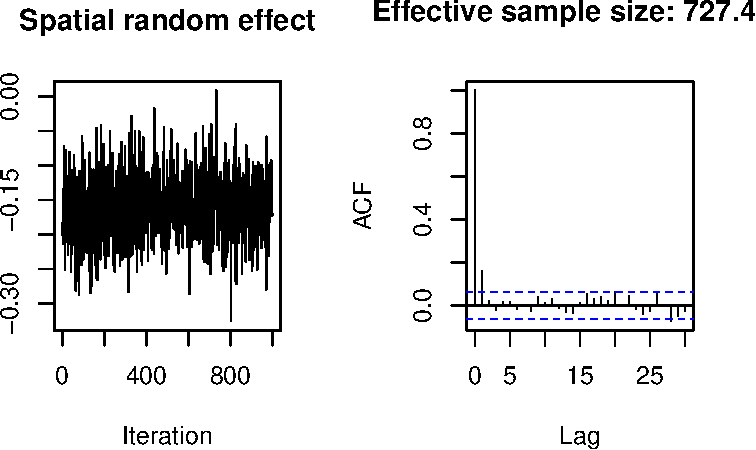
\includegraphics[keepaspectratio]{03_model-fitting_files/figure-pdf/fig-check-mcmc-mean-1.pdf}}

}

\caption{\label{fig-check-mcmc-mean}Trace plot (left panel) and
autocorrelation function plot (right panel) for the averaged spatial
random effects from the river-blindness data analysis. The title of the
right panel also shows the effective sample size of the 1000 Markov
chain Monte Carlo (MCMC) samples. The MCMC samples are obtained by
running the MCMC algorithm for 12000 iterations, with a burn-in of 2000
and thinning of 10.}

\end{figure}%

The plot shown in Figure~\ref{fig-check-mcmc-mean} are for the MCMC
samples of the averaged spatial random effect, that is
\(\bar{S} = \sum_{i=1}^n S(x_i) /n\). Performing the check on
\(\bar{S}\) is done to avoid the need of checking the convergence for
each individual component \(S(x_i)\). However, one of the risks of doing
this is that if fewer components of \(\bar{S}\) have not reached
convergence this may not be shown through the inspection of the samples
for \(\bar{S}\). However, this is an unlikely scenario when using the
type of MCMC algorithm implemented in \texttt{RiskMap} (see
Section~\ref{sec-mcmc-mala}). Nonetheless, if one wants to check the
convergence for individual components this can be done as follows.

\begin{Shaded}
\begin{Highlighting}[]
\FunctionTok{check\_mcmc}\NormalTok{(fit\_liberia, }\AttributeTok{check\_mean =} \ConstantTok{FALSE}\NormalTok{, }\AttributeTok{component =} \DecValTok{10}\NormalTok{)}
\end{Highlighting}
\end{Shaded}

\begin{figure}[H]

\centering{

\pandocbounded{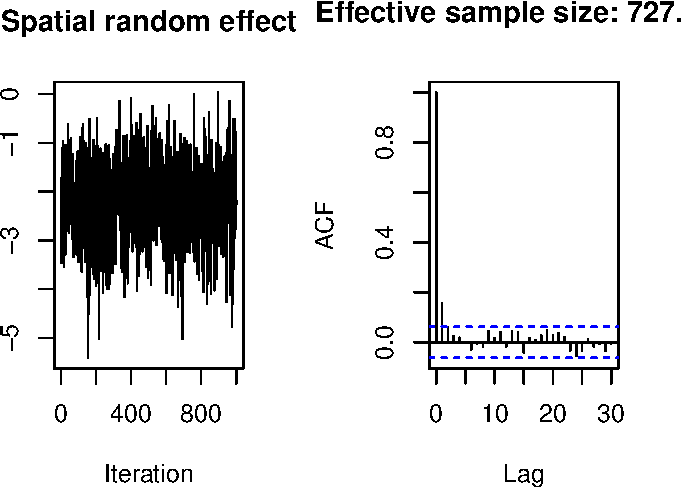
\includegraphics[keepaspectratio]{03_model-fitting_files/figure-pdf/fig-check-comp10-mcmc-1.pdf}}

}

\caption{\label{fig-check-comp10-mcmc}Trace plot (left panel) and
autocorrelation function plot (right panel) for the tenth component of
the spatial random effects from the river-blindness data analysis.}

\end{figure}%

Both Figure~\ref{fig-check-mcmc-mean} and
Figure~\ref{fig-check-comp10-mcmc}, shows a reasonably good mixing and
relatively low correlation in the samples. We point out that the number
of MCMC samples in \texttt{glgpm} are set through the function
\texttt{set\_control\_sim} passed to the argument
\texttt{control\_mcmc}. By default \texttt{set\_control\_sim} uses 12000
iterations, a burn-in of 2000 and thinning of 10, thus giving 1000 MCMC
samples. This configuration can be enough for the first run of the Monte
Carlo maximum Likelihood (MCML) method, however it is advisable to
increase the number of iterations to obtain a larger number of samples
with reduced correlation.

\begin{Shaded}
\begin{Highlighting}[]
\CommentTok{\# Update the guesses for the model parameters }
\NormalTok{par0\_liberia }\OtherTok{\textless{}{-}} \FunctionTok{coef}\NormalTok{(fit\_liberia)}

\CommentTok{\# Refit the model and increase the MCMC samples}
\NormalTok{fit\_liberia2 }\OtherTok{\textless{}{-}} 
\FunctionTok{glgpm}\NormalTok{(npos }\SpecialCharTok{\textasciitilde{}} \FunctionTok{log}\NormalTok{(elevation) }\SpecialCharTok{+} \FunctionTok{gp}\NormalTok{(long, lat, }\AttributeTok{nugget =} \ConstantTok{NULL}\NormalTok{),}
      \AttributeTok{den =}\NormalTok{ ntest, }\AttributeTok{data =}\NormalTok{ liberia,}
      \AttributeTok{crs =} \DecValTok{4326}\NormalTok{,}
      \AttributeTok{convert\_to\_crs =} \DecValTok{32629}\NormalTok{,}
      \AttributeTok{par0 =}\NormalTok{ par0\_liberia, }
      \AttributeTok{control\_mcmc =} \FunctionTok{set\_control\_sim}\NormalTok{(}\AttributeTok{n\_sim =} \DecValTok{110000}\NormalTok{, }
                                     \AttributeTok{burnin =} \DecValTok{10000}\NormalTok{, }
                                     \AttributeTok{thin =} \DecValTok{10}\NormalTok{),}
      \AttributeTok{family =} \StringTok{"binomial"}\NormalTok{, }\AttributeTok{messages =} \ConstantTok{FALSE}\NormalTok{)}
\end{Highlighting}
\end{Shaded}

\begin{Shaded}
\begin{Highlighting}[]
\FunctionTok{check\_mcmc}\NormalTok{(fit\_liberia2)}
\end{Highlighting}
\end{Shaded}

\begin{figure}[H]

\centering{

\pandocbounded{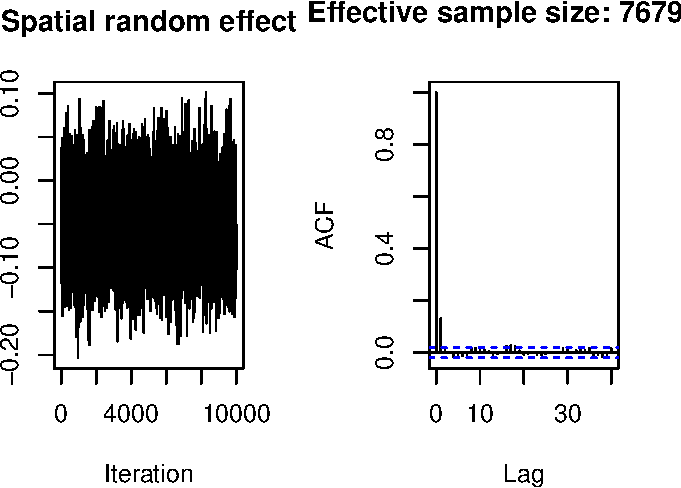
\includegraphics[keepaspectratio]{03_model-fitting_files/figure-pdf/fig-mcmc-10k-1.pdf}}

}

\caption{\label{fig-mcmc-10k}Trace plot (left panel) and autocorrelation
function plot (right panel) for the tenth component of the spatial
random effects from the river-blindness data analysis. The Markov chain
Monte Carlo (MCMC) samples are obtained by running the MCMC algorithm
for 110000 iterations, with a burn-in of 10000 and thinning of 10.}

\end{figure}%

The code above performs an additional step in the MCML estimation, using
10,000 MCMC samples. As shown in Figure~\ref{fig-mcmc-10k}, these MCMC
samples exhibit good mixing and low autocorrelation, which indicates
that they adequately approximate the likelihood function of the Binomial
geostatistical model. Although additional MCMC iterations could be run
to obtain estimates closer to the true maximum likelihood estimate
(since we are approximating the likelihood function and not obtaining
the exact MLE), we choose not to do so here. This decision is due to
both the computational time required and the minimal impact of Monte
Carlo error on spatial predictions in this case.

\subsubsection{Alternative approaches}\label{alternative-approaches}

In the sections above, we focused specifically on the implementation of
the Monte Carlo Maximum Likelihood (MCML) method in \texttt{RiskMap}.
However, other approaches are available, some of which are
computationally more efficient than the MCML method we have illustrated.
Our preference for this estimation method is based on two main reasons:
1) it delivers robust performance across a wide range of data scenarios,
and 2) it does not require the specification of arbitrary prior
distributions when prior information on the model parameters is
unavailable.

Alternative methods worth mentioning include the
expectation-maximization algorithm for maximum likelihood estimation
(Zhang 2002), integrated nested Laplace approximation (INLA) (Rue,
Martino, and Chopin 2009), and implementations of the
Metropolis-Adjusted Langevin Algorithm (MALA) for Bayesian inference (O.
Christensen, Roberts, and Sköld 2006). While these methods are valuable,
explaining and comparing them is not our focus here, as it would detract
from the practical orientation of this book.

\subsection{The Hat matrix in linear geostatistical
models}\label{sec-h-matrix}

We consider the geostatistical model

\[
Y_i = d(x_i)^\top \beta + S(x_i) + Z_i
\]

where \$ Y\_i \$ is the observed response at location \$ x\_i \$, \$
d(x\_i) \$ is a \$ p \$-dimensional vector of covariates, \$ \beta \$ is
a \$ p \times 1 \$ vector of regression coefficients, \$ S(x\_i) \$ is a
spatially structured random effect, and \$ Z\_i \sim N(0, \tau\^{}2) \$
is independent Gaussian noise. The model can be rewritten as

\[
Y = D\beta + S + Z
\]

where \$ Y = (Y\_1, \ldots, Y\_n)\top \$ is the \$ n \times 1 \$ vector
of observations, \$ S = (S(x\_1), \ldots, S(x\_n))\^{}\top \$ is the
vector of spatially dependent random effects, \(Z = (Z_1, \ldots, Z_n)\)
is the noise, and \$ D \$ is an \$ n \times p \$ matrix of covariates
given by

\[
D = (d_1(X), \ldots, d_p(X))
\]

with each column \$ d\_j(X) = (d\_j(x\_1),\ldots,d\_j(x\_n))\top \$
representing the values of the \$ j \$-th covariate across all
locations. This formulation accounts for both fixed effects through \$
D\beta \$ and spatial correlation through \$ S(x\_i) \$. The covariance
matrix of \$ Y \$ is

\[
V = \Sigma + \tau^2 I
\]

where \$ \Sigma \$ is the spatial covariance matrix of \(S\). Assuming
the covariance parameters are known, the generalized least squares
estimator for \$ \beta \$ is

\[
\hat{\beta} = (D^T V^{-1} D)^{-1} D^T V^{-1} Y.
\]

The predictor for \(S\) is the the conditional expectation
\(E[S(x_i) \: | \: Y_i]\) is

\[
\hat{S} = \Sigma V^{-1} (Y - D\hat{\beta}).
\]

so the predictors for \(Y\) can be written as

\[
\hat{Y} = D\hat{\beta} + \hat{S}.
\]

The hat matrix, which projects observations onto the fitted space, is

\[
H = [D - \Sigma V^{-1} D] (D^T V^{-1} D)^{-1} D^T V^{-1} + \Sigma V^{-1}.
\]

This matrix is symmetric since it consists of symmetric components,
satisfying \(H^T = H\). It is also idempotent, meaning \(H^2 = H\),
which follows from the properties of projection matrices. The diagonal
elements \(h_{ii}\) represent the leverage of each observation,
quantifying how much each \$ Y\_i \$ influences its own fitted value.
The rank of \$ H \$ is at most \$ p \$, constrained by the rank of \$ D
\$. Unlike in ordinary least squares where the hat matrix is
\(H = D (D^T D)^{-1} D^T\), here it depends on \(V^{-1}\), accounting
for spatial dependence. Since \(V \neq I\), the hat matrix represents an
oblique projection rather than an orthogonal one.

The residuals, i.e.~the estimate of \(Z\) are given by

\[
\hat{Z} = Y - \hat{Y} = (I - H) Y.
\]

We not thet the covariance structure of \(\hat{Z}\) is

\[
\text{Var}(\hat{Z}) = (I - H) V (I - H)^T.
\]

Hence, the estimated residuals from a linear geostatistical model do
have a correlation structure which relates to the chosen spatial
correlation structure in \(\Sigma\).

\section{Review questions}\label{review-questions-1}

\begin{itemize}
\item
  Describe how you would perform exploratory analysis between counts
  data and covariates, distnsuighing between unbounded counts
  (e.g.~Poisson), bounded counts (e.g.~Binomial) and binary outcomes.
\item
  Define the theoretical and empirical variogram, making appropriate use
  of equations.
\item
  How do we use the empirical variogram to test for spatial correlation?
  What are the limitations of this approach?
\item
  Define the class of generalized linear geostatistical models and list
  all the assumptions.
\item
  Explain intuitively what are the computational challenges related to
  the fit of geostatistical models and what approaches can be used for
  parameter estimation.
\end{itemize}

\section{Exercises}\label{exercises-1}

\begin{enumerate}
\def\labelenumi{\arabic{enumi}.}
\item
  Consider the Binomial mixed model with linear predictor as defined in
  Equation~\ref{eq-linear-predictor-glmms-ch2}. By editing the code for
  the simulation shown in Section~\ref{sec-overdispersion}, generate a
  graph as in Figure~\ref{fig-var-bin-glmm} under the two following
  scenarios: \(i\)) \(\tau^2 = 0.2\) and \(n_i=100\); \(ii\))
  \(\tau^2 = 0.1\) and \(n_i = 1\). How does the variance of \(Y_i\)
  change under \(i\)) and \(ii\)) in comparison to
  Figure~\ref{fig-var-bin-glmm}? How do you explain the differences?
\item
  Similarly to the previous exercise, consider a Poisson mixed model
  with linear predictor \[
      \log\left\{\mu_i\right\} = \beta_0 + Z_i,
      \] where \(Z_i\) are a set of mutually independent Gaussian
  variables with mean 0 and variance \(\tau^2\). Using the code shown in
  Section~\ref{sec-overdispersion}, carry out a simulation study to
  compute the variance of \(Y_i\) and generate a graph similar to
  Figure~\ref{fig-var-bin-glmm} to compare the variance of the Poisson
  mixed model with that of a standard Poisson model. Generate the graph
  for different values of \(\tau^2\) and summarize your findings. NOTE:
  In this simulation the offset \(n_i\) can be set to 1.
\item
  Create an R function that computes the \emph{cloud variogram}. As
  explained in Section~\ref{sec-expl-spatial}, the cloud variogram is
  obtained by plotting \(\hat{V}_{ij}\) (see
  Equation~\ref{eq-hat-squared-diff}) against the distances \(u_{ij}\).
  The function should take as input a data-set with three columns: the
  variable for which the cloud variogram is to be computed; and two
  columns corresponding to the location of the data. Then, use this
  function to create the cloud variogram for the model for
  river-blindness in Equation~\ref{eq-liberia-bin-mixed-elev}. How does
  this compare to empirical variogram that takes the averages within
  predefined distance classes, as shown in
  Figure~\ref{fig-liberia-variog}?
\item
  Fit a Binomial mixed model to the Liberia data-set on river-blindness
  without any covariates, i.e.~\[
      \log\left\{\frac{p(x_i)}{1-p(x_i)}\right\} = \beta_0 + Z_i.
      \] Making use of the R code presented in
  Section~\ref{sec-empirical-variog-bin}, use the function
  \texttt{s\_variogram} to generate the empirical variogram for this
  model and compare this to the empirical variogram of
  Figure~\ref{fig-liberia-variog}. What differences do you observe?
\item
  Fit a Poisson mixed model to the anopheles mosquito data using
  elevation as a covariate, i.e.~\[
      \log\{\mu(x_i)\} = \beta_{0} + \beta_{1} d(x_i) + Z_i
      \] where \(d(x_i)\) is the measured elevation at location \(x_i\).
  How strong is the overdispersion in the data? After fitting the model,
  extract the estimates of the random effects \(Z_i\) and compute the
  empirical variogram with the 95\% envelope for spatial independence.
  Repeat this for different classes of distances by changing the input
  passed to \texttt{bins} in the \texttt{s\_variogram} function. How do
  the different specifications of \texttt{bins} affect the results?
\item
  \emph{Parametric bootstrap.} Using the model fitted to the Anopheles
  gambiae mosquitoes in Section~\ref{sec-anopheles-fit}, simulate 1000
  data-sets using the \texttt{glgpm\_sim} function and estimate the
  model to each of the simulated data-set. Use the resulting 1000
  estimates to compute 95\(\%\) confidence intervals for each of the
  model parameters and compare this with the confidence intervals
  obtained from the model summary.
\end{enumerate}

\bookmarksetup{startatroot}

\chapter{Geostatistical prediction}\label{sec-geo-prediction}

\section*{List of the main functions used in the
chapter}\label{list-of-the-main-functions-used-in-the-chapter-1}
\addcontentsline{toc}{section}{List of the main functions used in the
chapter}

\markright{List of the main functions used in the chapter}

\begin{longtable}[]{@{}
  >{\raggedright\arraybackslash}p{(\linewidth - 4\tabcolsep) * \real{0.3472}}
  >{\raggedright\arraybackslash}p{(\linewidth - 4\tabcolsep) * \real{0.2500}}
  >{\raggedright\arraybackslash}p{(\linewidth - 4\tabcolsep) * \real{0.4028}}@{}}
\toprule\noalign{}
\begin{minipage}[b]{\linewidth}\raggedright
Function
\end{minipage} & \begin{minipage}[b]{\linewidth}\raggedright
R Package
\end{minipage} & \begin{minipage}[b]{\linewidth}\raggedright
Used for
\end{minipage} \\
\midrule\noalign{}
\endhead
\bottomrule\noalign{}
\endlastfoot
\texttt{pred\_over\_grid} & \texttt{RiskMap} & Predicting the different
component of the linear predictor over a grid: the covariates effects
and the random effects \\
\texttt{pred\_target\_grid} & \texttt{RiskMap} & Predictions of target
defined at pixel-level \\
\texttt{pred\_target\_shp} & \texttt{RiskMap} & Predictions of targets
defined at areal level \\
\texttt{assess\_pp} & \texttt{RiskMap} & Assessing the predictive
performance of geostatistical models using cross-validation \\
\texttt{surf\_sim} & \texttt{RiskMap} & Simulating surfaces and data
from geostatistical models \\
\texttt{assess\_sim} & \texttt{RiskMap} & Assessing the predictive
performance of geostatistical models using simulations \\
\end{longtable}

Geostatistics was originally developed and applied as a predictive tool
for improving mining operations and planning. In the seminal paper on
model-based geostatistics (MBG) (P. J. Diggle, Tawn, and Moyeed 1998),
the authors begin by stating:

\begin{quote}
*``Conventional geostatistical methodology solves the problem of
predicting the realized value of a linear functional of a Gaussian
spatial stochastic process* \(S(x)\) based on observations
\(Y_i= S(x_i) + Z_i\) at sampling locations \(x_i\), where the \(Z_i\)
are mutually independent, zero-mean Gaussian random variables.''
\end{quote}

It is no coincidence that, although MBG represents a broad class of
statistical models applicable to both estimation and prediction
problems, the majority of its applications have focused on prediction.
This is evident in many scientific fields where MBG has been used,
including global public health, which is the primary application focus
in this book. In line with the quote above, for most of the examples
considered in this book, the analyses we illustrate aim to use a finite
set of locations \(x_i\) --- typically corresponding to households or
villages --- to make inferences about an observed disease risk surface.
Having performed estimation of MBG models in
Chapter~\ref{sec-estimation}, we can now carry out spatial prediction to
answer critical public health questions, such as identifying hot-spots
and cold-spots --- areas of unusually high or low disease risk,
respectively --- or determining whether the average prevalence across a
region exceeds a predefined policy threshold.

In this chapter, we will explore these issues, beginning with a formal
statistical formulation of the spatial prediction problem and a
description of the necessary steps for its implementation. We will then
demonstrate how spatial prediction is performed when considering
predictive targets at both the \emph{pixel-level} and
\emph{areal-level}. Finally, we will conclude the chapter by presenting
methods for comparing the predictive performance of different models,
with some insights into their relative strengths and weaknesses.

\section{Spatial prediction using geostatistical
models}\label{sec-spat-pred-target}

Let us consider the class of generalized linear geostatistical models
(GLGM) as in Section~\ref{sec-geostat-models}. In the formulation of
prediction problems, the first step consists of defining our predictive
target, which we denote as \(T(x)\) where \(x\) denotes any locations
within the study, which is usually not part of the sampled data. For
example in the analysis of the riverblindness in Liberia, our interest
lies in identifying areas where disease prevalence exceeds 20\(\%\), a
threshold that use been used in the past to identify areas in need of
mass drug administration due to the potential for significant disease
burden and transmission (Amazigo 2008). Hence, in this case, disease
prevalence corresponds to our predictive target \(T(x)\). To draw
inferences on \(T(x)\) and allow us to answer the question of where
\(T(x)\) exceeds a 20\(\%\) threshold, we first need to obtain the so
called \emph{predictive distribution} of \(T(x)\). More specifically,
the \emph{predictive distribution} of \(T(x)\) is the distribution of
\(T(x)\) conditioned to the data, which we denote by
\([T(x) \: \mid \: y]\). More importantly, by incorporating the
information provided by the data, the predictive distribution of the
target enables us to quantify the uncertainty stemming from the
stochastic nature of the process we are modeling. In other words, the
predictive distribution reflects the range of possible values that the
target \(T(x)\) can take and their likelihoods based on the model we
have fitted to the data. As we shall see in our examples, we can use the
predictive distribution of \(T(x)\) both to provide what is our ``best
guess'' for \(T(x)\) and a summary of uncertainty which quantifies how
much concentrated is the predictive distribution around that guess.
However, providing a single ``best guess'' for \(T(x)\) is not always
the answer to our research question. In the example on riverblindness
mentioned at the start of the this section, a more natural way to use
the predictive distribution would be to compute the likelihood that
\(T(x)\) exceeds 0.2 at any given location \(x\).

In summary, the first two steps of spatial prediction are:

\begin{itemize}
\item
  Step 1. define the predictive target \(T(x)\);
\item
  Step 2. obtain the predictive distribution of \(T(x)\) and use this to
  compute summaries that helps to answer your original research
  question.
\end{itemize}

This begs two practical questions: ``How do we obtain the predictive
distribution of \(T(x)\)?'' and ``How do we use the predictive
distribution to compute our summaries?''. For a mathematical derivation
of the predictive distribution and the form that this takes in the
special case of a linear geostatistical model, you can read
Section~\ref{sec-theory-prediction}. In what follows, we shall assume
that we can simulate directly from \([T(x) \: \mid \: y]\) either using
direct simulation or Markov Chains Monte Carlo (see
Section~\ref{sec-mcmc-mala}).

In our exposition so far, we have also made the implicit assumption that
prediction is required for our predictive target at a single, unsampled,
location \(x\) and for this reason we have denote our predictive target
simply as \(T(x)\). However, this is almost never the case, since in
most cases, our predictive target correspond to either of the following.

\begin{itemize}
\item
  \textbf{Spatially continuous targets} correspond to an unobserved
  spatially continuous surface (e.g.~disease prevalence), formally
  denoted by \(\mathcal{T} = \{T(x), x \in A\}\), where \(A\) is our
  region of interest.
\item
  \textbf{Areal-level targets}, usually defined as transformation of the
  spatially continuous surface \(\mathcal{T}\), defined previously, and
  which we denote as \(\mathcal{T}_{A} = F(\mathcal{T}, A)\). For
  example, the average of \(T(x)\) over \(A\) is an areal-level target,
  formally defined as \(F(\mathcal{T}, A) = \int_{A} T(x) \: dx / |A|\),
  where \(|A|\) is the area of \(A\).
\end{itemize}

Before we consider these two types of prediction targets more in detail,
we first explain the preliminary steps that need to be performed and are
common to both. Whether our goal is predict a spatially continuous or
areal-level target, the initial task is to draw Monte Carlo samples from
the predictive distribution of the spatial process \(S(x)\). Next, we
define a set of prediction locations, say \(q\) in total, denoted as
\(\tilde{X} = {\tilde{x}_1, \ldots, \tilde{x}_q}\). These locations
correspond to a regular grid that spans our region of interest, \(A\).
the predictive distribution of the spatial process over the grid,
represented as \([S(\tilde{X}) \: |\: y]\). This distribution allows us
to generate Monte Carlo samples for \(S(\tilde{X})\), which will later
be used for computing our target.

\begin{tcolorbox}[enhanced jigsaw, leftrule=.75mm, rightrule=.15mm, breakable, opacityback=0, coltitle=black, toprule=.15mm, toptitle=1mm, colbacktitle=quarto-callout-note-color!10!white, bottomrule=.15mm, opacitybacktitle=0.6, arc=.35mm, colback=white, title=\textcolor{quarto-callout-note-color}{\faInfo}\hspace{0.5em}{Note}, colframe=quarto-callout-note-color-frame, titlerule=0mm, bottomtitle=1mm, left=2mm]

Here, we are overlooking the fact that when \(T(x)\) is a linear
transformation of \(S(x)\) and the the model fitted to the data is a
linear geostatistical model, then we can derive any summary of the
predictive distribution analytically, without the need of carrying out
any simulation. Although this may displease some of our fellow
statisticians who care about computational efficiency, for pedagogical
reasons, here we have chosen to explain only the Monte Carlo based
approach, which works in all scenarios.

\end{tcolorbox}

At this stage, we need to consider which of the two following types of
predictions from \([S(\tilde{X}) \: |\: y]\) are required.

\begin{itemize}
\item
  \textbf{Marginal predictions} are obtained by simulating independently
  from the \(q\) marginal predictive distributions of
  \([S(\tilde{X}) | y]\). In other words, we consider a prediction
  location \(\tilde{x}_j\), simulate from \([S(\tilde{x}_j) \: |\: y]\)
  say \(B\) samples, and repeat this for \(j=1,\ldots,q\)
\item
  \textbf{Joint predictions} are obtained by simulating from the joint
  distribution of \([S(\tilde{X}) \: |\: y]\). Unlike marginal
  predictions, joint predictions take into account the correlation
  between the different components of \([S(\tilde{X}) \: |\: y]\).
\end{itemize}

To better understand the technical differences between marginal and
joint predictions, we refer you to Section~\ref{sec-pred-distr-theory}.
However, in practice, the two following observations are important.

O1. Joint predictions are computationally more intensive than marginal
predictions.

O2. Joint predictions are required when the predictive target is at
areal-level.

O3. For spatially continuous targets, both marginal and joint
predictions can be used but, in light of O1, we might prefer using the
former.

\subsection{\texorpdfstring{Generating samples from the predictive
distribution of \(S(\tilde{X})\) (continue from
Section~\ref{sec-liberia-estim1})}{Generating samples from the predictive distribution of S(\textbackslash tilde\{X\}) (continue from Section~)}}\label{sec-pred-samples}

We now show how the ideas and concepts discussed above are put into
practice in an geostatistical analysis, using the Liberia data example.
Using the fitted model in Section~\ref{sec-liberia-estim1}, we use the
\texttt{predict\_over\_grid} function in \texttt{RiskMap}, to sample
from the predictive distribution of the spatial Gaussian process
\(S(x)\) based on a regular grid spanning the country of Liberia.

The \texttt{pred\_over\_grid} function enables us to predict the the
separate effects of the covariates, given by \(d(x)^\top \beta\), and
the spatial random effects, \(S(x)\), at any desired location \(x\).
Hence, before we can use the \texttt{pred\_over\_grid} function, we need
to do 1) obtain a shape file that defines the boundaries of our study
area, 2) use that to create a regular grid and 3) extract the covariates
values at those locations. The R script below performs all these steps.

\begin{Shaded}
\begin{Highlighting}[]
\CommentTok{\# 1) Obtaining Liberia boundaries }
\FunctionTok{library}\NormalTok{(rgeoboundaries)}
\NormalTok{liberia\_adm0 }\OtherTok{\textless{}{-}} \FunctionTok{geoboundaries}\NormalTok{(}\StringTok{"liberia"}\NormalTok{, }\AttributeTok{adm\_lvl =} \StringTok{"adm0"}\NormalTok{)}
\NormalTok{liberia\_adm0 }\OtherTok{\textless{}{-}} \FunctionTok{st\_transform}\NormalTok{(liberia\_adm0, }\AttributeTok{crs =} \DecValTok{32629}\NormalTok{)}

\CommentTok{\# 2) Create the grid at 5 km resolution}
\NormalTok{liberia\_grid }\OtherTok{\textless{}{-}} \FunctionTok{create\_grid}\NormalTok{(liberia\_adm0, }\AttributeTok{spat\_res =} \DecValTok{5}\NormalTok{)}

\CommentTok{\# Download elevation data}
\FunctionTok{library}\NormalTok{(elevatr)}
\NormalTok{liberia\_elev }\OtherTok{\textless{}{-}} \FunctionTok{get\_elev\_raster}\NormalTok{(}\AttributeTok{locations =}\NormalTok{ liberia\_adm0, }
                                \AttributeTok{z =} \DecValTok{5}\NormalTok{, }\AttributeTok{clip =} \StringTok{"locations"}\NormalTok{)}

\CommentTok{\# 3) Extracting elevation at the grid locations}
\NormalTok{lb\_predictors }\OtherTok{\textless{}{-}} \FunctionTok{data.frame}\NormalTok{(}\AttributeTok{elevation =} 
\NormalTok{                         terra}\SpecialCharTok{::}\FunctionTok{extract}\NormalTok{(liberia\_elev,}
                                \FunctionTok{st\_coordinates}\NormalTok{(liberia\_grid)))}
\end{Highlighting}
\end{Shaded}

In the code above, we generated a prediction grid --- which, we recall,
that we denote as \(\tilde{X}\) --- with a spatial resolution of 5 km.
Generally, a higher spatial resolution (note that a ``higher spatial
resolution'' corresponds to a lower value for \texttt{spat\_res}) yields
more detailed prediction maps but also increases the computational cost.
In this case, the choice of a 5 km grid strikes a balance between
sufficient visualization clarity and manageable computation time.

At this point, we have all the necessary inputs to execute the
\texttt{pred\_over\_grid} function for both marginal and joint
predictions, as demonstrated below.

\begin{Shaded}
\begin{Highlighting}[]
\CommentTok{\# Predicting the spatial process S(x) over the grid, as well as}
\CommentTok{\# covariates effects}

\CommentTok{\# Marginal predictions}
\NormalTok{lb\_pred\_S\_m }\OtherTok{\textless{}{-}} \FunctionTok{pred\_over\_grid}\NormalTok{(fit\_liberia, }
                            \AttributeTok{grid\_pred =}\NormalTok{ liberia\_grid, }
               \AttributeTok{predictors =}\NormalTok{ lb\_predictors, }\AttributeTok{messages =} \ConstantTok{FALSE}\NormalTok{,}
               \AttributeTok{type =} \StringTok{"marginal"}\NormalTok{)}

\CommentTok{\# Joint predictions}
\NormalTok{lb\_pred\_S\_j }\OtherTok{\textless{}{-}} \FunctionTok{pred\_over\_grid}\NormalTok{(fit\_liberia, }
                            \AttributeTok{grid\_pred =}\NormalTok{ liberia\_grid, }
               \AttributeTok{predictors =}\NormalTok{ lb\_predictors, }\AttributeTok{messages =} \ConstantTok{FALSE}\NormalTok{,}
               \AttributeTok{type =} \StringTok{"joint"}\NormalTok{)}
\end{Highlighting}
\end{Shaded}

Both \texttt{lb\_pred\_S\_m} and \texttt{lb\_pred\_S\_j} contain lists
with the same arguments, with one key difference: the samples in the
list element named \texttt{S\_samples} for the former are drawn from the
marginal predictive distributions of the components of \(S(\tilde{X})\),
while for the latter, they come from the joint predictive distribution
of \(S(\tilde{X})\).

An important note is that in the code above we have used the default
settings for the Markov Chain Monte Carlo (MCMC). To change these
setting use the function \texttt{set\_control\_sim} whose output should
be passed to the argument \texttt{contol\_sim} of
\texttt{pred\_over\_grid}. The diagnostic on the convergence of the MCMC
can also be applying the \texttt{check\_mcmc} function to either
\texttt{lb\_pred\_S\_m} or \texttt{lb\_pred\_S\_j}; see
Section~\ref{sec-summary} for more details.

We can inspect the predictive distribution of any component
\(S(\tilde{X})\) through the Monte Carlo samples stored in
\texttt{S\_samples}. For example, the script below generates the
histogram for the predictive distribution of the first component of
\(S(\tilde{X})\) (Figure~\ref{fig-hist-first-comp-pd}).

\begin{Shaded}
\begin{Highlighting}[]
\FunctionTok{hist}\NormalTok{(lb\_pred\_S\_m}\SpecialCharTok{$}\NormalTok{S\_samples[,}\DecValTok{1}\NormalTok{], }\AttributeTok{main =} \StringTok{"Predictive distribution"}\NormalTok{,}
     \AttributeTok{xlab =} \FunctionTok{expression}\NormalTok{(}\FunctionTok{S}\NormalTok{(}\FunctionTok{tilde}\NormalTok{(x)[}\DecValTok{1}\NormalTok{])))}
\end{Highlighting}
\end{Shaded}

\begin{figure}[H]

\centering{

\pandocbounded{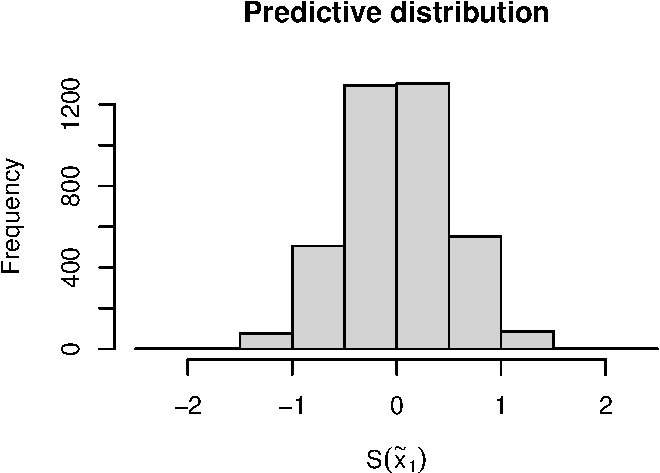
\includegraphics[keepaspectratio]{04_geostatistical-prediction_files/figure-pdf/fig-hist-first-comp-pd-1.pdf}}

}

\caption{\label{fig-hist-first-comp-pd}Histrogram of the predictive
distribution of the first component, \(S(\tilde{x}_1)\) of
\(S(\tilde{X})\) for the Liberia data analysis.}

\end{figure}%

\section{Spatially continuous targets}\label{sec-spat-cont-target}

In the previous section, we explained and demonstrated how to obtain
Monte Carlo samples from the predictive distribution of
\(S(\tilde{X})\), which we denoted by \([S(\tilde{X}) \: |\: y]\). Let
\(S_{(j)}(\tilde{X})\) and \([S(\tilde{X}) \: |\: y]\) represent the
\(j\)-th Monte Carlo samples for the entire grid and the specific
location \(x_k\), respectively, for \(j=1,\ldots,B\) and
\(k=1,\ldots,q\).

We define our predictive target, \(T(x)\), at any given location \(x\),
as a transformation of \(S(x)\). Thus, we express it as
\(T(x) = f\{S(x)\}\). Note that \(f(\cdot)\) can represent any type of
non-linear transformation of \(S(x)\) and may include covariate effects
and other non-structured random effects. A list of common predictive
targets frequently used in geostatistical analysis is provided in
Table~\ref{tbl-spat-cont-pred-target}.

\begin{longtable}[]{@{}
  >{\raggedright\arraybackslash}p{(\linewidth - 4\tabcolsep) * \real{0.3836}}
  >{\raggedright\arraybackslash}p{(\linewidth - 4\tabcolsep) * \real{0.3014}}
  >{\raggedright\arraybackslash}p{(\linewidth - 4\tabcolsep) * \real{0.3151}}@{}}
\caption{List of some of the most common spatially continuous predictive
targets in a geostatistical analysis. For each target, we also indicate
the generalized linear model (GLM) family for which these can be
defined. Note that this list not exhaustive and different predictive
other than those listed in the table could also be
considered.}\label{tbl-spat-cont-pred-target}\tabularnewline
\toprule\noalign{}
\begin{minipage}[b]{\linewidth}\raggedright
Predictive target \(T(x)\)
\end{minipage} & \begin{minipage}[b]{\linewidth}\raggedright
Name of the predictive target
\end{minipage} & \begin{minipage}[b]{\linewidth}\raggedright
Generalized linear model (GLM) family
\end{minipage} \\
\midrule\noalign{}
\endfirsthead
\toprule\noalign{}
\begin{minipage}[b]{\linewidth}\raggedright
Predictive target \(T(x)\)
\end{minipage} & \begin{minipage}[b]{\linewidth}\raggedright
Name of the predictive target
\end{minipage} & \begin{minipage}[b]{\linewidth}\raggedright
Generalized linear model (GLM) family
\end{minipage} \\
\midrule\noalign{}
\endhead
\bottomrule\noalign{}
\endlastfoot
\(d(x)^\top \beta + S(x)\) & Linear predictor & Any GLM \\
\(\frac{\exp\{d(x)^\top \beta + S(x)\}}{1+\exp\{d(x)^\top \beta + S(x)\}}\)
& Prevalence & Binomial \\
\(\exp\{d(x)^\top \beta + S(x)\}\) & Mean number of cases & Poisson \\
\(S(x)\) & Spatial random effects & Any GLM \\
\(d(x)^\top \beta\) & Covariates effects & Any GLM \\
\end{longtable}

An important feature of the predictive targets listed in
Table~\ref{tbl-spat-cont-pred-target} is that none of them include the
nugget effect, denoted by \(Z_i\) in our linear predictor definition for
generalized linear geostatistical models. The reason for excluding
\(Z_i\) from the predictive targets is that, in most cases, it lacks a
clear, unambiguous scientific interpretation. However, \(Z_i\) might be
included, for example, in environmental studies focusing on highly
localized phenomena where measurement error or small-scale variability
is of direct scientific interest; or in epidemiological studies where
inferences at the individual level, rather than the population level,
are required, and where \(Z_i\) is introduced to account for unexplained
individual-level variation. It is also worth noticing, the primary
impact of including \(Z_i\) in \(T(x)\) would be an increase in the
uncertainty of predictive inferences for \(T(x)\), with minimal effect
(or none at all, if \(T(x)\) corresponds to the linear predictor) on the
point predictions.

The predictive targets in Table~\ref{tbl-spat-cont-pred-target}
corresponding to \(d(x)^\top \beta\) or the spatial random effects
\(S(x)\) might be considered when the goal is to highlight the different
contribution to the overall predictive inferences from the measured
covariates.

\subsection{\texorpdfstring{Example: mapping riverblidness prevalence in
Liberia (continuing from
Section~\ref{sec-pred-samples})}{Example: mapping riverblidness prevalence in Liberia (continuing from Section~)}}\label{sec-liberia-prediction-1}

Let us continue the geostatistical of the riverblindness data in
Liberia. The predictive target we consider is prevalence, hence
\begin{equation}\phantomsection\label{eq-rb-prev-target}{T(x) = \frac{\exp\{ \beta_{0} + \beta_{1}\log\{e(x)\} + S(x)\}}{1+\exp\{\beta_{0} + \beta_{1}\log\{e(x)\} + S(x)\}},}\end{equation}
where \(e(x)\) is the elevation in meters at location \(x\).

Through the \texttt{pred\_target\_grid} we can use the output in
\texttt{lb\_pred\_S\_m} (or \texttt{lb\_pred\_S\_j} as well, in this
case) to generate predictions of prevalence over the regular grid at 5
km we have created earlier.

\begin{Shaded}
\begin{Highlighting}[]

\CommentTok{\# Prediction of riverblindness prevalence}
\NormalTok{lb\_prev }\OtherTok{\textless{}{-}} 
\FunctionTok{pred\_target\_grid}\NormalTok{(}
\NormalTok{  lb\_pred\_S\_m, }
  \AttributeTok{f\_target =} \FunctionTok{list}\NormalTok{(}\AttributeTok{prev =} \ControlFlowTok{function}\NormalTok{(lp) }\FunctionTok{exp}\NormalTok{(lp)}\SpecialCharTok{/}\NormalTok{(}\DecValTok{1}\SpecialCharTok{+}\FunctionTok{exp}\NormalTok{(lp))),}
  \AttributeTok{pd\_summary =} \FunctionTok{list}\NormalTok{(}\AttributeTok{mean =} \ControlFlowTok{function}\NormalTok{(Tx) }\FunctionTok{mean}\NormalTok{(Tx), }
                    \AttributeTok{cv =} \ControlFlowTok{function}\NormalTok{(Tx) }\FunctionTok{sd}\NormalTok{(Tx)}\SpecialCharTok{/} \FunctionTok{mean}\NormalTok{(Tx),}
                    \AttributeTok{exceed20 =} \ControlFlowTok{function}\NormalTok{(Tx) }\FunctionTok{mean}\NormalTok{(Tx }\SpecialCharTok{\textgreater{}} \FloatTok{0.2}\NormalTok{))}
\NormalTok{)}
\end{Highlighting}
\end{Shaded}

In the function above the argument \texttt{f\_target} can take a list of
functions, as multiple predictive targets can be defined. Here, we only
specified prevalence (\texttt{prev}). Note that in defining the
predictive target in \texttt{f\_target}, we need to express that as a
function of \(d(x)^\top \beta + S(x)\). The argument
\texttt{include\_covariates} also allows us to define predictive target
that do not use covariates from the model. By default
\texttt{include\_covariates\ =\ TRUE}, hence in the code above
covariates are part of what is defined as \texttt{lp}. To predict the
spatial random effects \(S(x)\) only, for example, you can set
\texttt{include\_covariates\ =\ FALSE} and
\texttt{f\_target\ =\ list(Sx\ =\ function(lp)\ lp)}. In
\texttt{pd\_summary}, we define the summaries that we want to visualize
from the predictive distribution. Here, we have specified the mean,
coefficient of variation and the probability of exceeding a 20\(\%\)
prevalence threshold.

We can then visualize the resulting maps as follows.

\begin{Shaded}
\begin{Highlighting}[]
\CommentTok{\# Displying the results}
\FunctionTok{par}\NormalTok{(}\AttributeTok{mfrow =} \FunctionTok{c}\NormalTok{(}\DecValTok{1}\NormalTok{,}\DecValTok{3}\NormalTok{))}
\FunctionTok{plot}\NormalTok{(lb\_prev, }\AttributeTok{which\_target =} \StringTok{"prev"}\NormalTok{, }
     \AttributeTok{which\_summary =} \StringTok{"mean"}\NormalTok{, }\AttributeTok{main =} \StringTok{"Mean"}\NormalTok{)}
\FunctionTok{plot}\NormalTok{(lb\_prev, }\AttributeTok{which\_target =} \StringTok{"prev"}\NormalTok{, }
     \AttributeTok{which\_summary =} \StringTok{"cv"}\NormalTok{, }\AttributeTok{main =} \StringTok{"Coefficient of variation"}\NormalTok{)}
\FunctionTok{plot}\NormalTok{(lb\_prev, }\AttributeTok{which\_target =} \StringTok{"prev"}\NormalTok{, }
     \AttributeTok{which\_summary =} \StringTok{"exceed20"}\NormalTok{, }\AttributeTok{main =} \StringTok{"Exceedance probability"}\NormalTok{)}
\FunctionTok{par}\NormalTok{(}\AttributeTok{mfrow=}\FunctionTok{c}\NormalTok{(}\DecValTok{1}\NormalTok{,}\DecValTok{1}\NormalTok{))}
\end{Highlighting}
\end{Shaded}

\begin{figure}[H]

\centering{

\pandocbounded{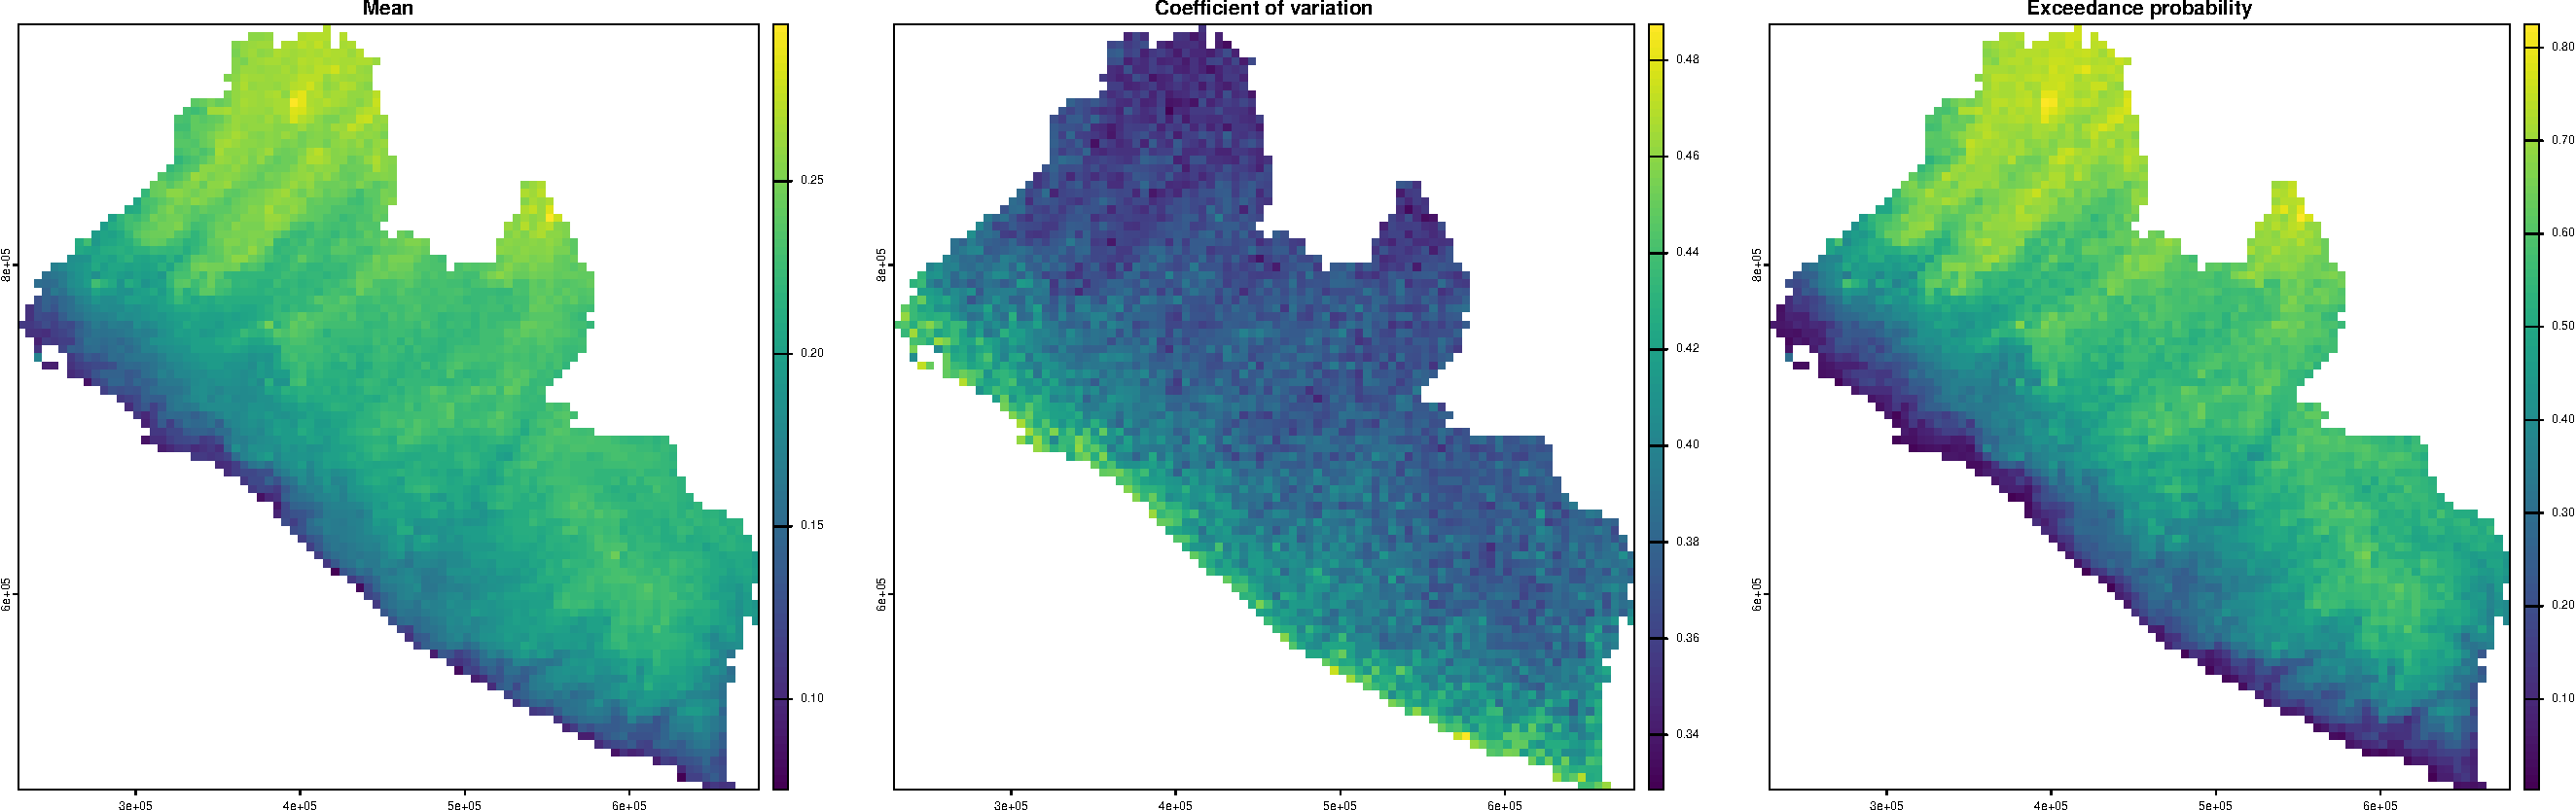
\includegraphics[keepaspectratio]{04_geostatistical-prediction_files/figure-pdf/fig-lb-maps-1.pdf}}

}

\caption{\label{fig-lb-maps}Mapping riverblindness in Liberia. Plots of
the mean (left panel), coefficient of variation (central panel) and
exceedance probability (right panel) for a 20\% prevalence threshold.}

\end{figure}%

The maps in Figure~\ref{fig-lb-maps} indicate a higher prevalence as we
move away from the coast and at higher altitudes. A very similar spatial
pattern is observed in the likelihood of exceeding 20\(\%\) prevalence.
Also, based on the map of the coefficient of variation, the uncertainty
around the point predictions of prevalence is higher along the coast and
lower in the inland areas of Liberia.

\subsection{Example: mapping malaria using age and elevation as
predictors}\label{sec-non-spar-covariates}

We now consider an example on malaria mapping, where we use two
different types of covariates: a spatially referenced covariate
corresponding to elevation; the individual age. We use the
\texttt{malkenya\_comm} subset of the \texttt{malkenya} data-set (see
Section~\ref{sec-indiv-expl-analysis}) and, to alleviate the
computational burden, we further reduce this data-set by taking the
first 1000 rows. Hence, we create our new data-set,
\texttt{malkenya\_comm1000}, using the followind code.

\begin{Shaded}
\begin{Highlighting}[]
\NormalTok{malkenya\_comm1000 }\OtherTok{\textless{}{-}}\NormalTok{ malkenya\_comm[}\DecValTok{1}\SpecialCharTok{:}\DecValTok{1000}\NormalTok{,]}

\NormalTok{malkenya\_comm1000 }\OtherTok{\textless{}{-}} \FunctionTok{st\_as\_sf}\NormalTok{(malkenya\_comm1000, }\AttributeTok{coords =} \FunctionTok{c}\NormalTok{(}\StringTok{"Long"}\NormalTok{, }\StringTok{"Lat"}\NormalTok{),}
                              \AttributeTok{crs =} \DecValTok{4326}\NormalTok{)}
\NormalTok{malkenya\_comm1000 }\OtherTok{\textless{}{-}} \FunctionTok{st\_transform}\NormalTok{(malkenya\_comm1000, }\AttributeTok{crs =} \DecValTok{32736}\NormalTok{)}
\end{Highlighting}
\end{Shaded}

Based on the exploratory analysis shown in
Section~\ref{sec-indiv-expl-analysis}, we consider a geostatistical
model fitted to the individual binary outcomes, \(Y_{ij}\), which
correspond the rapid diagnostic test (RDT) results for the \(j\)-th
individual in the \(i\)-th community, and take value \(Y_{ij}=1\) if the
RDT is positive and \(Y_{ij}=0\) if the RDT is negative. Using a
Binomial geostatistical model, we model the individual probability,
\(p_{ij}\) of a positive RDT using the following linear predictor.
\begin{equation}\phantomsection\label{eq-lp-malkenya}{
\log\left\{\frac{p_{ij}}{1-p_{ij}}\right\} = \beta_{0} + \beta_{1}a_{ij}+\beta_{2} \times\max\{a_{ij}-15, 0\} + \beta_{3}\max\{a_{ij}-40, 0\} + \beta_{4} e(x_i) + S(x_i),
}\end{equation} where \(e(x_{i})\) and \(a_{ij}\) are the elevation in
meter and the age in years for the \(j\)-th individual residing at the
\(i\)-th household, respectively.

When using the model in Equation~\ref{eq-lp-malkenya} to predict RDT
prevalence, a key question arises: how should we handle the age
variable, which, unlike elevation, is not available as a geo-referenced
covariate at all locations in the study area? The answer depends on the
research question being addressed.

For instance, if the goal is to infer disease risk across different age
groups, we can generate different maps for each group of interest. This
can be easily achieved by fixing the value of \(a_{ij}\) to a specific
age for all prediction locations. Alternatively, if the objective is to
generate a predictive map for the general population, rather than for a
specific age group, we must employ a probabilistic model for age and
integrate out its effect.

Developing a credible probabilistic model for age is beyond the scope of
this section. Instead, we demonstrate a simple yet reasonable solution
which uses the empirical age distribution from the data. By random
sampling from this distribution, we can then assign age values to
prediction locations. The steps are as follows.

\begin{enumerate}
\def\labelenumi{\arabic{enumi}.}
\tightlist
\item
  Obtain the empirical distribution of age from the data.
\item
  Sample with replacement from such distribution (the \texttt{sample}
  function in R can be used for this purpose) as many times as the
  number of prediction locations, so that each grid location
  \(\tilde{x}\) has a value of age assigned.
\item
  Generate a sample from the predictive distribution of the target
  \(T(\tilde{x})\) at each of the grid locations \(\tilde{x}\).
\item
  Repeat 1 to 3, for as many times as the samples generates from
  \(S(\tilde{X})\).
\end{enumerate}

This approach relies on two key assumptions. First, that the age
distribution is spatially neutral, i.e., it does not vary across space.
Second, that the data are representative of the age distribution in the
target population. In the data used for this example, we believe these
assumptions are reasonable, given the relatively small study area, where
age is unlikely to exhibit significant spatial variation, and the fact
that the data are a random sample from the community.

In the scripts presented in the remainder of this section, we show how
to generate a predictive map of prevalence for children age 15 years,
and another map that instead uses the approach earlier described to
remove the effect of age and generate a map of prevalence for the
general population.

First, we fit the model. Note that the effect of age is not linear and
we use linear splines to account for this, using the results of the
exploratory analysis shown in @Section~\ref{sec-indiv-expl-analysis}.

\begin{Shaded}
\begin{Highlighting}[]
\NormalTok{fit\_malkenya }\OtherTok{\textless{}{-}} \FunctionTok{glgpm}\NormalTok{(RDT }\SpecialCharTok{\textasciitilde{}}\NormalTok{ Age }\SpecialCharTok{+}  \FunctionTok{pmax}\NormalTok{(Age}\DecValTok{{-}15}\NormalTok{, }\DecValTok{0}\NormalTok{) }\SpecialCharTok{+} 
                        \FunctionTok{pmax}\NormalTok{(Age}\DecValTok{{-}40}\NormalTok{, }\DecValTok{0}\NormalTok{) }\SpecialCharTok{+}\NormalTok{ elevation }\SpecialCharTok{+}
                        \FunctionTok{gp}\NormalTok{(),}
                      \AttributeTok{data =}\NormalTok{ malkenya\_comm1000,}
                      \AttributeTok{family =} \StringTok{"binomial"}\NormalTok{)}
\end{Highlighting}
\end{Shaded}

After fitting the model, we create a prediction grid at a spatial
resolution of 500 meters and extract the values of elevation. In this
analysis, due to the small size of the study area, we do not use
administrative boundaries as they are too large. Instead, we use the
convex hull of the sample locations to define the boundaries of our
study area.

\begin{tcolorbox}[enhanced jigsaw, leftrule=.75mm, rightrule=.15mm, breakable, opacityback=0, coltitle=black, toprule=.15mm, toptitle=1mm, colbacktitle=quarto-callout-note-color!10!white, bottomrule=.15mm, opacitybacktitle=0.6, arc=.35mm, colback=white, title=\textcolor{quarto-callout-note-color}{\faInfo}\hspace{0.5em}{Note}, colframe=quarto-callout-note-color-frame, titlerule=0mm, bottomtitle=1mm, left=2mm]

The convex hull of a set of spatial locations is the smallest possible
shape (usually a polygon) that completely encloses all the points, such
that if you take any two points inside the shape, the straight line
connecting them is also entirely inside the shape. In simple terms, it
can be thought of as stretching a rubber band around the outermost
points in a set, and the shape the rubber band forms is the convex hull.

\end{tcolorbox}

\begin{Shaded}
\begin{Highlighting}[]
\CommentTok{\# Create grid from convex hull}
\NormalTok{shp\_ch }\OtherTok{\textless{}{-}} \FunctionTok{convex\_hull\_sf}\NormalTok{(malkenya\_comm1000)}
\NormalTok{ken\_grid }\OtherTok{\textless{}{-}} \FunctionTok{create\_grid}\NormalTok{(shp\_ch, }\AttributeTok{spat\_res =} \FloatTok{0.5}\NormalTok{)}

\CommentTok{\# Get elevation raster}
\NormalTok{ken\_elev }\OtherTok{\textless{}{-}} 
\FunctionTok{get\_elev\_raster}\NormalTok{(}\AttributeTok{locations =}\NormalTok{ shp\_ch, }
                \AttributeTok{z =} \DecValTok{9}\NormalTok{, }\AttributeTok{clip =} \StringTok{"locations"}\NormalTok{)}
\end{Highlighting}
\end{Shaded}

We then create the data frame of predictors where age is set to 15.

\begin{Shaded}
\begin{Highlighting}[]
\CommentTok{\# Create the data fr}
\NormalTok{ken\_predictors }\OtherTok{\textless{}{-}} \FunctionTok{data.frame}\NormalTok{(}\AttributeTok{elevation =} 
                           \FunctionTok{extract}\NormalTok{(ken\_elev, }\FunctionTok{st\_coordinates}\NormalTok{(ken\_grid)),}
                         \AttributeTok{Age =} \DecValTok{15}\NormalTok{)}
\end{Highlighting}
\end{Shaded}

We now have all the ingredients to carry out prediction.

\begin{Shaded}
\begin{Highlighting}[]
\NormalTok{pred\_ken\_S }\OtherTok{\textless{}{-}} \FunctionTok{pred\_over\_grid}\NormalTok{(fit\_malkenya, }\AttributeTok{grid\_pred =}\NormalTok{ ken\_grid,}
                             \AttributeTok{predictors =}\NormalTok{ ken\_predictors)}

\NormalTok{pred\_age15 }\OtherTok{\textless{}{-}} 
\FunctionTok{pred\_target\_grid}\NormalTok{(pred\_ken\_S, }
                 \AttributeTok{f\_target =} \FunctionTok{list}\NormalTok{(}\AttributeTok{prev =} \ControlFlowTok{function}\NormalTok{(lp) }\FunctionTok{exp}\NormalTok{(lp)}\SpecialCharTok{/}\NormalTok{(}\DecValTok{1}\SpecialCharTok{+}\FunctionTok{exp}\NormalTok{(lp))),}
                 \AttributeTok{pd\_summary =} \FunctionTok{list}\NormalTok{(}\AttributeTok{mean =} \ControlFlowTok{function}\NormalTok{(Tx) }\FunctionTok{mean}\NormalTok{(Tx)))}
\end{Highlighting}
\end{Shaded}

The code below shows how to perform the 4 steps described above to
generate a predictive map for the general population. Below we use the
function \texttt{update\_predictors} to update the covariates effects
that are stored in \texttt{mu\_pred}, a list element generated as the
output of \texttt{pred\_over\_grid}.

\begin{Shaded}
\begin{Highlighting}[]
\CommentTok{\# Number of Monte Carlo samples}
\NormalTok{n\_sim }\OtherTok{\textless{}{-}} \FunctionTok{ncol}\NormalTok{(pred\_age15}\SpecialCharTok{$}\NormalTok{lp\_samples)}

\CommentTok{\# Number of prediction locations}
\NormalTok{n\_pred }\OtherTok{\textless{}{-}} \FunctionTok{nrow}\NormalTok{(predictors)}

\CommentTok{\# The create object \textasciigrave{}pred\_ken\_S\_i\textasciigrave{} with the goal of changing the }
\CommentTok{\# coviariates effects stored in \textasciigrave{}mu\_pred\textasciigrave{} according the sample values of age}
\NormalTok{pred\_ken\_S\_i }\OtherTok{\textless{}{-}}\NormalTok{ pred\_ken\_S}
\NormalTok{pred\_ken\_S\_i}\SpecialCharTok{$}\NormalTok{mu\_pred }\OtherTok{\textless{}{-}} \FunctionTok{matrix}\NormalTok{(}\ConstantTok{NA}\NormalTok{, }\AttributeTok{nrow =}\NormalTok{ n\_pred, }\AttributeTok{ncol =}\NormalTok{ n\_sim)}

\ControlFlowTok{for}\NormalTok{(i }\ControlFlowTok{in} \DecValTok{1}\SpecialCharTok{:}\NormalTok{n\_sim) \{}
  \CommentTok{\# Generate n\_pred samples from the empirical distribution of age}
\NormalTok{  ken\_predictors}\SpecialCharTok{$}\NormalTok{Age }\OtherTok{\textless{}{-}} \FunctionTok{sample}\NormalTok{(malkenya\_comm1000}\SpecialCharTok{$}\NormalTok{Age, n\_pred, }\AttributeTok{replace =} \ConstantTok{TRUE}\NormalTok{)}
  \CommentTok{\# Generate the new covariates effects with \textasciigrave{}update\_predictors\textasciigrave{} and store them in }
  \CommentTok{\# \textasciigrave{}mu\_pred\textasciigrave{}}
\NormalTok{  pred\_ken\_S\_i}\SpecialCharTok{$}\NormalTok{mu\_pred[,i] }\OtherTok{\textless{}{-}} \FunctionTok{update\_predictors}\NormalTok{(pred\_ken\_S, ken\_predictors)}\SpecialCharTok{$}\NormalTok{mu\_pred}
\NormalTok{\}}

\CommentTok{\# Prediction of prevalence}
\NormalTok{pred\_aver\_pop }\OtherTok{\textless{}{-}} \FunctionTok{pred\_target\_grid}\NormalTok{(pred\_ken\_S\_i, }
               \AttributeTok{f\_target =} \FunctionTok{list}\NormalTok{(}\AttributeTok{prev =} \ControlFlowTok{function}\NormalTok{(lp) }\FunctionTok{exp}\NormalTok{(lp)}\SpecialCharTok{/}\NormalTok{(}\DecValTok{1}\SpecialCharTok{+}\FunctionTok{exp}\NormalTok{(lp))))}
\end{Highlighting}
\end{Shaded}

We can now plot the two maps and compare them.

\begin{Shaded}
\begin{Highlighting}[]
\FunctionTok{par}\NormalTok{(}\AttributeTok{mfrow =} \FunctionTok{c}\NormalTok{(}\DecValTok{1}\NormalTok{,}\DecValTok{2}\NormalTok{))}
\FunctionTok{plot}\NormalTok{(pred\_age15, }\AttributeTok{which\_target =} \StringTok{"prev"}\NormalTok{, }\AttributeTok{which\_summary =} \StringTok{"mean"}\NormalTok{, }\AttributeTok{main =} \StringTok{"Prevalence (15 years)"}\NormalTok{, }\AttributeTok{range =} \FunctionTok{c}\NormalTok{(}\DecValTok{0}\NormalTok{,}\FloatTok{0.6}\NormalTok{))}
\FunctionTok{plot}\NormalTok{(pred\_aver\_pop, }\AttributeTok{which\_target =} \StringTok{"prev"}\NormalTok{, }\AttributeTok{which\_summary =} \StringTok{"mean"}\NormalTok{,  }\AttributeTok{main =} \StringTok{"Prevalence (General population)"}\NormalTok{, }\AttributeTok{range =} \FunctionTok{c}\NormalTok{(}\DecValTok{0}\NormalTok{,}\FloatTok{0.6}\NormalTok{))}
\FunctionTok{par}\NormalTok{(}\AttributeTok{mfrow =} \FunctionTok{c}\NormalTok{(}\DecValTok{1}\NormalTok{,}\DecValTok{1}\NormalTok{))}
\end{Highlighting}
\end{Shaded}

\begin{figure}[H]

\centering{

\pandocbounded{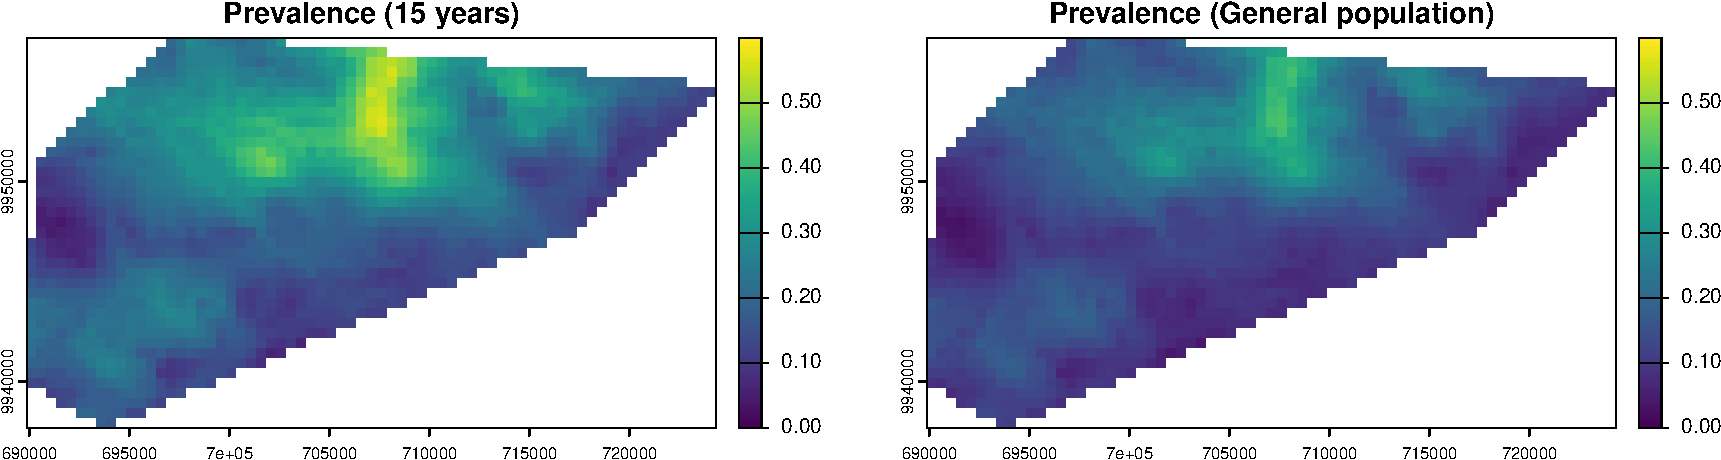
\includegraphics[keepaspectratio]{04_geostatistical-prediction_files/figure-pdf/fig-malaria-maps-1.pdf}}

}

\caption{\label{fig-malaria-maps}Maps of the predictive mean of the
rapid diagnostic test (RDT) prevalence for children of the age of 15
(left panel) and the general population (right panel).}

\end{figure}%

The exploratory analysis of Section~\ref{sec-indiv-expl-analysis} had
shown that the prevalence around the age of 15 is higher than at other
ages. This is also reflected in Figure~\ref{fig-malaria-maps}, when the
left panel, corresponding to the RDT prevalence for children at the age
of 15 years, shows a higher level of prevalence than the right panel,
which is instead for the general population.

\section{Areal-level targets}\label{sec-areal-target}

When determining areal-level targets, we must first address the
following questions:

\begin{enumerate}
\def\labelenumi{\arabic{enumi}.}
\tightlist
\item
  What spatially continuous target, \(T(x)\), are we seeking to
  aggregate?
\item
  What are the spatial units, denoted as \(A_i\) for
  \(i = 1, \dots, N\), over which the aggregation is required?
\item
  What aggregating function should be applied?
\item
  Should spatial weights be incorporated in the aggregation, and if so,
  what weights are appropriate?
\end{enumerate}

The first question was discussed in earlier sections, where examples of
predictive targets that define \(T(x)\) can be found in
Table~\ref{tbl-spat-cont-pred-target}. The answers to the remaining
questions are context-dependent and closely linked to the primary
research objectives. In public health settings, the areas \(A_i\) often
correspond to administrative units or regions where decisions are made
and resources are allocated.

A common aggregating function for \(T(x)\) is the mean, which is
formally defined as:

\begin{equation}\phantomsection\label{eq-mean-alt}{
\mathcal{M}_i = \frac{1}{|A_i|}\int_{A_i} T(x) \: dx.
}\end{equation}

In addition to the mean, several other aggregating functions can be
applied depending on the context of the analysis. We also note that
computing the integral in Equation~\ref{eq-mean-alt} requires some
approximations. Our approach utilizes the regular grid \(\tilde{X}\),
previously defined when dealing with spatially continuous targets. This
grid covers the area \(A_i\), allowing us to approximate \(M_i\) as:
\begin{equation}\phantomsection\label{eq-mean-alt-approx}{\mathcal{M}_i \approx \frac{1}{\#\{j : \tilde{x}_j \in A_i\}} \sum_{\tilde{x}_j \in A_i} T(\tilde{x}_j), }\end{equation}
where \(\#\{j : \tilde{x}_j \in A_i\}\) denotes the number of grid
locations \(\tilde{x}_j\) that fall within \(A_i\). The same
approximation will be applied to other areal-level targets discussed in
this section. However, for simplicity, we will omit the detailed
explanation of this step and instead express the predictive target as an
integral.

For instance, in the study of Anopheles mosquitoes in Cameroon, we may
be interested in estimating the total number of mosquitoes trapped
within the study area (\(A_i\) represents a single region in this case).
If \(T(x)\) denotes the number of mosquitoes trapped at location \(x\),
the areal-level target can be expressed as: \[
  \mathcal{S}_i = \int_{A_i} T(x) \: dx.
  \]

Additionally, to capture the heterogeneity of \(T(x)\) within an area,
variance-based measures can be used. The variance of \(T(x)\) in \(A_i\)
is given by: \[
   \mathcal{V}_i = \frac{1}{|A_i|}\int_{A_i} \left(T(x) - \mathcal{M}_i\right)^2 \: dx,
   \] where \(\mathcal{M}_i\) is the mean of \(T(x)\) in \(A_i\).

The formulation of the areal-level targets given so far assumes equal
weighting for all locations within the area. Alternatively, if the we
consider for example the areal level target in
Equation~\ref{eq-mean-alt}, one could use spatial weights, \(w(x) > 0\),
and redefine \(\mathcal{M}_i\) as:

\[
\mathcal{M}_i = \frac{\int_{A_i} w(x) T(x) \: dx}{\int_{A_i} w(x) \: dx}.
\]

Selecting appropriate spatial weights is crucial, as it reflects the
significance of different locations within the area. We can define three
types of weighting: population-density, risk-based, and distance-based.
We point out that this distinction is not always clear cut (population
could indeed be a risk factor in our analysis) but this classification
is made only for the sake of making the explanation clearer.

For example, if the goal is to prioritize areas with higher populations,
weights \(w(x)\) could be proportional to population density at location
\(x\). This approach gives greater importance to locations where more
people reside, which can be particularly relevant when aggregating
disease prevalence data for resource allocation.

In cases where certain sub-regions within \(A_i\) are at higher risk for
disease (e.g., proximity to environmental hazards or areas with lower
access to healthcare), risk-based weights could be applied. Here,
\(w(x)\) would be higher in regions identified as higher risk, providing
a more targeted aggregation of disease prevalence. For example,
populations in rural areas may face higher exposure to infectious
diseases than those in urban areas, making it important to assign
greater weight to these higher-risk regions in the aggregation process.

If the objective is to account for proximity effects (such as the spread
of an infectious disease or contamination from a known source),
distance-based weights could be used. Locations closer to a known
disease outbreak area or source of exposure could be given more weight
to reflect the spatial dynamics of disease transmission.

Using spatial weights in these ways ensures that the aggregation of
disease prevalence \(T(x)\) reflects not only the distribution of the
disease but also the underlying population, risk, or spatial
characteristics relevant to the public health problem under
investigation.

\subsection{\texorpdfstring{Example: predicting the average
riverblindness prevalence at admin level 1 in Liberia (continuing from
Section~\ref{sec-liberia-prediction-1})}{Example: predicting the average riverblindness prevalence at admin level 1 in Liberia (continuing from Section~)}}\label{sec-liberia-prediction-2}

We continue our analysis of the Liberia data and consider areal-level
targets. More specifically, we aim to predict the average prevalence
over the regions which give the administrative level 1 of Liberia. By
denoting with \(A_i\) the i-th out of the 15 regions in Liberia. By
denoting with \(T(x)\) reiverblindness prevalence as defined in
Equation~\ref{eq-rb-prev-target}, we define our predictive target as \[
T_{i} = \frac{1}{|A_i|} \int_{A_i} T(x) \: dx.
\] The R code below shows how predictions for \(T_i\) can be performed
using the \texttt{pred\_target\_shp} function.

\begin{Shaded}
\begin{Highlighting}[]
\CommentTok{\# Admin level 1 boundaries}
\FunctionTok{library}\NormalTok{(rgeoboundaries)}
\NormalTok{lb\_adm1 }\OtherTok{\textless{}{-}} \FunctionTok{geoboundaries}\NormalTok{(}\AttributeTok{country =} \StringTok{"Liberia"}\NormalTok{, }\AttributeTok{adm\_lvl =} \StringTok{"adm1"}\NormalTok{)}

\CommentTok{\# Prediction of prevalence }
\NormalTok{pred\_shp }\OtherTok{\textless{}{-}} \FunctionTok{pred\_target\_shp}\NormalTok{(lb\_pred\_S\_j, }\AttributeTok{shp =}\NormalTok{ lb\_adm1,}
                            \AttributeTok{shp\_target =} \ControlFlowTok{function}\NormalTok{(Tx) }\FunctionTok{mean}\NormalTok{(Tx),}
                            \AttributeTok{f\_target =} \FunctionTok{list}\NormalTok{(}\AttributeTok{prev =} 
                                       \ControlFlowTok{function}\NormalTok{(lp) }\FunctionTok{exp}\NormalTok{(lp)}\SpecialCharTok{/}\NormalTok{(}\DecValTok{1}\SpecialCharTok{+}\FunctionTok{exp}\NormalTok{(lp))),}
                            \AttributeTok{pd\_summary =} \FunctionTok{list}\NormalTok{(}\AttributeTok{mean =}\NormalTok{ mean),}
                            \AttributeTok{col\_names =} \StringTok{"shapeName"}\NormalTok{)}
\end{Highlighting}
\end{Shaded}

The argument \texttt{shp\_target} is used define the type of aggregation
function over the region \(A_i\), in this case the mean of the target
\(T(x)\). Also note that, like for spatially continuous targets, we can
define any summary of the predictive distribution of \(\mathcal{M}_i\)
through the argument \texttt{pd\_summary}. Here, we chose to compute
only the mean of the predictive distribution but other summaries, such
as exceedance probabilities, standard error, quantiles and so on, can be
specified if needed.

Before we plot the results on a map, let us also consider the
population-density weighted target, defined as \[
T_{i}^* = \frac{ \int_{A_i} w(x) T(x) \: dx}{\int_{A_i} w(x) \: dx}.
\] To aid the explanation of the R code script, we first rewrite the
above areal-level target as \[
T_{i}^* = \int_{A_i} \tilde{w_i}(x) T(x) \: dx.
\] where \(\tilde{w}_{i}(x)\) are the standardized weights that
integrate to 1 in \(A_i\)
(i.e.~\(\int_{A_i} \tilde{w}_i(x) \: dx = 1\)).

We first retrieve the population density data from the World Pop
database (see Section~\ref{sec-pop-data}) and use these to derive the
un-standardized weights \(w(x)\).

\begin{Shaded}
\begin{Highlighting}[]

\CommentTok{\# Obtaining population density}
\FunctionTok{library}\NormalTok{(wpgpDownloadR)}
\NormalTok{lbr\_url }\OtherTok{\textless{}{-}} \FunctionTok{wpgpGetCountryDataset}\NormalTok{(}\AttributeTok{ISO3 =} \StringTok{"LBR"}\NormalTok{, }\AttributeTok{covariate =} \StringTok{"ppp\_2014"}\NormalTok{)}
\FunctionTok{library}\NormalTok{(terra)}
\NormalTok{lbr\_pop }\OtherTok{\textless{}{-}} \FunctionTok{rast}\NormalTok{(lbr\_url)}
\NormalTok{lbr\_pop }\OtherTok{\textless{}{-}} \FunctionTok{project}\NormalTok{(lbr\_pop, }\StringTok{"EPSG:32629"}\NormalTok{)}

\CommentTok{\# Extra pop density weights at the prediction grid}
\NormalTok{weights\_pred }\OtherTok{\textless{}{-}} \FunctionTok{extract}\NormalTok{(lbr\_pop, }\FunctionTok{st\_coordinates}\NormalTok{(liberia\_grid))}\SpecialCharTok{$}\NormalTok{lbr\_ppp\_2014}
\end{Highlighting}
\end{Shaded}

In the code above the population density weights are extracted at the
locations of the prediction grid. In the \texttt{pred\_target\_shp}
function, in order to use the weights for our predictive target, we need
to specify two additional arguments: \texttt{weights} to which we pass
the population density values (in our case these are stored in
\texttt{weights\_pred}); \texttt{standardize\_weights}, which is a
logical argument taking value \texttt{TRUE} if the weights to be
standardized so that the sum over the grid covering a region \(A_i\)
adds up to one.

\begin{Shaded}
\begin{Highlighting}[]
\NormalTok{pred\_shp\_w }\OtherTok{\textless{}{-}} \FunctionTok{pred\_target\_shp}\NormalTok{(lb\_pred\_S\_j, }\AttributeTok{shp =}\NormalTok{ lb\_adm1,}
                            \AttributeTok{shp\_target =} \ControlFlowTok{function}\NormalTok{(Tx) }\FunctionTok{sum}\NormalTok{(Tx),}
                            \AttributeTok{f\_target =} \FunctionTok{list}\NormalTok{(}\AttributeTok{prev =} 
                                       \ControlFlowTok{function}\NormalTok{(lp) }\FunctionTok{exp}\NormalTok{(lp)}\SpecialCharTok{/}\NormalTok{(}\DecValTok{1}\SpecialCharTok{+}\FunctionTok{exp}\NormalTok{(lp))),}
                            \AttributeTok{pd\_summary =} \FunctionTok{list}\NormalTok{(}\AttributeTok{mean =}\NormalTok{ mean),}
                            \AttributeTok{weights =}\NormalTok{ weights\_pred,}
                            \AttributeTok{standardize\_weights =} \ConstantTok{TRUE}\NormalTok{,}
                            \AttributeTok{col\_names =} \StringTok{"shapeName"}\NormalTok{)}
\end{Highlighting}
\end{Shaded}

We can then finally plot the results from the prediction at admin level
1, without using any weights and by weighing according to population
density.

\begin{Shaded}
\begin{Highlighting}[]
\NormalTok{plot\_1 }\OtherTok{\textless{}{-}} 
\FunctionTok{plot}\NormalTok{(pred\_shp, }\AttributeTok{which\_target =} \StringTok{"prev"}\NormalTok{, }\AttributeTok{which\_summary =} \StringTok{"mean"}\NormalTok{,}
     \AttributeTok{palette =} \StringTok{"RdYlGn"}\NormalTok{,}
    \AttributeTok{limits =} \FunctionTok{c}\NormalTok{(}\FloatTok{0.1}\NormalTok{, }\FloatTok{0.30}\NormalTok{),}
    \AttributeTok{breaks =} \FunctionTok{seq}\NormalTok{(}\FloatTok{0.1}\NormalTok{,}\FloatTok{0.30}\NormalTok{, }\AttributeTok{by =} \FloatTok{0.05}\NormalTok{)) }\SpecialCharTok{+} 
  \FunctionTok{guides}\NormalTok{(}\AttributeTok{fill=}\FunctionTok{guide\_legend}\NormalTok{(}\AttributeTok{title=}\StringTok{"Prevalence"}\NormalTok{)) }\SpecialCharTok{+}
  \FunctionTok{ggtitle}\NormalTok{(}\StringTok{"Average prevalence }\SpecialCharTok{\textbackslash{}n}\StringTok{ (no weights)"}\NormalTok{) }\SpecialCharTok{+} 
   \FunctionTok{theme}\NormalTok{(}\AttributeTok{plot.title =} \FunctionTok{element\_text}\NormalTok{(}\AttributeTok{size =} \DecValTok{15}\NormalTok{))}

\NormalTok{plot\_2  }\OtherTok{\textless{}{-}} 
  \FunctionTok{plot}\NormalTok{(pred\_shp\_w, }\AttributeTok{which\_target =} \StringTok{"prev"}\NormalTok{, }\AttributeTok{which\_summary =} \StringTok{"mean"}\NormalTok{,}
     \AttributeTok{palette =} \StringTok{"RdYlGn"}\NormalTok{,}
    \AttributeTok{limits =} \FunctionTok{c}\NormalTok{(}\FloatTok{0.1}\NormalTok{, }\FloatTok{0.30}\NormalTok{),}
    \AttributeTok{breaks =} \FunctionTok{seq}\NormalTok{(}\FloatTok{0.1}\NormalTok{,}\FloatTok{0.30}\NormalTok{, }\AttributeTok{by =} \FloatTok{0.05}\NormalTok{)) }\SpecialCharTok{+} 
  \FunctionTok{guides}\NormalTok{(}\AttributeTok{fill=}\FunctionTok{guide\_legend}\NormalTok{(}\AttributeTok{title=}\StringTok{"Prevalence"}\NormalTok{)) }\SpecialCharTok{+}
  \FunctionTok{ggtitle}\NormalTok{(}\StringTok{"Average prevalence }\SpecialCharTok{\textbackslash{}n}\StringTok{ (population weighted)"}\NormalTok{) }\SpecialCharTok{+} 
  \FunctionTok{theme}\NormalTok{(}\AttributeTok{plot.title =} \FunctionTok{element\_text}\NormalTok{(}\AttributeTok{size =} \DecValTok{15}\NormalTok{))}

\FunctionTok{library}\NormalTok{(gridExtra)}
\FunctionTok{grid.arrange}\NormalTok{(plot\_1, plot\_2, }\AttributeTok{ncol =} \DecValTok{2}\NormalTok{)}
\end{Highlighting}
\end{Shaded}

\begin{figure}[H]

\centering{

\pandocbounded{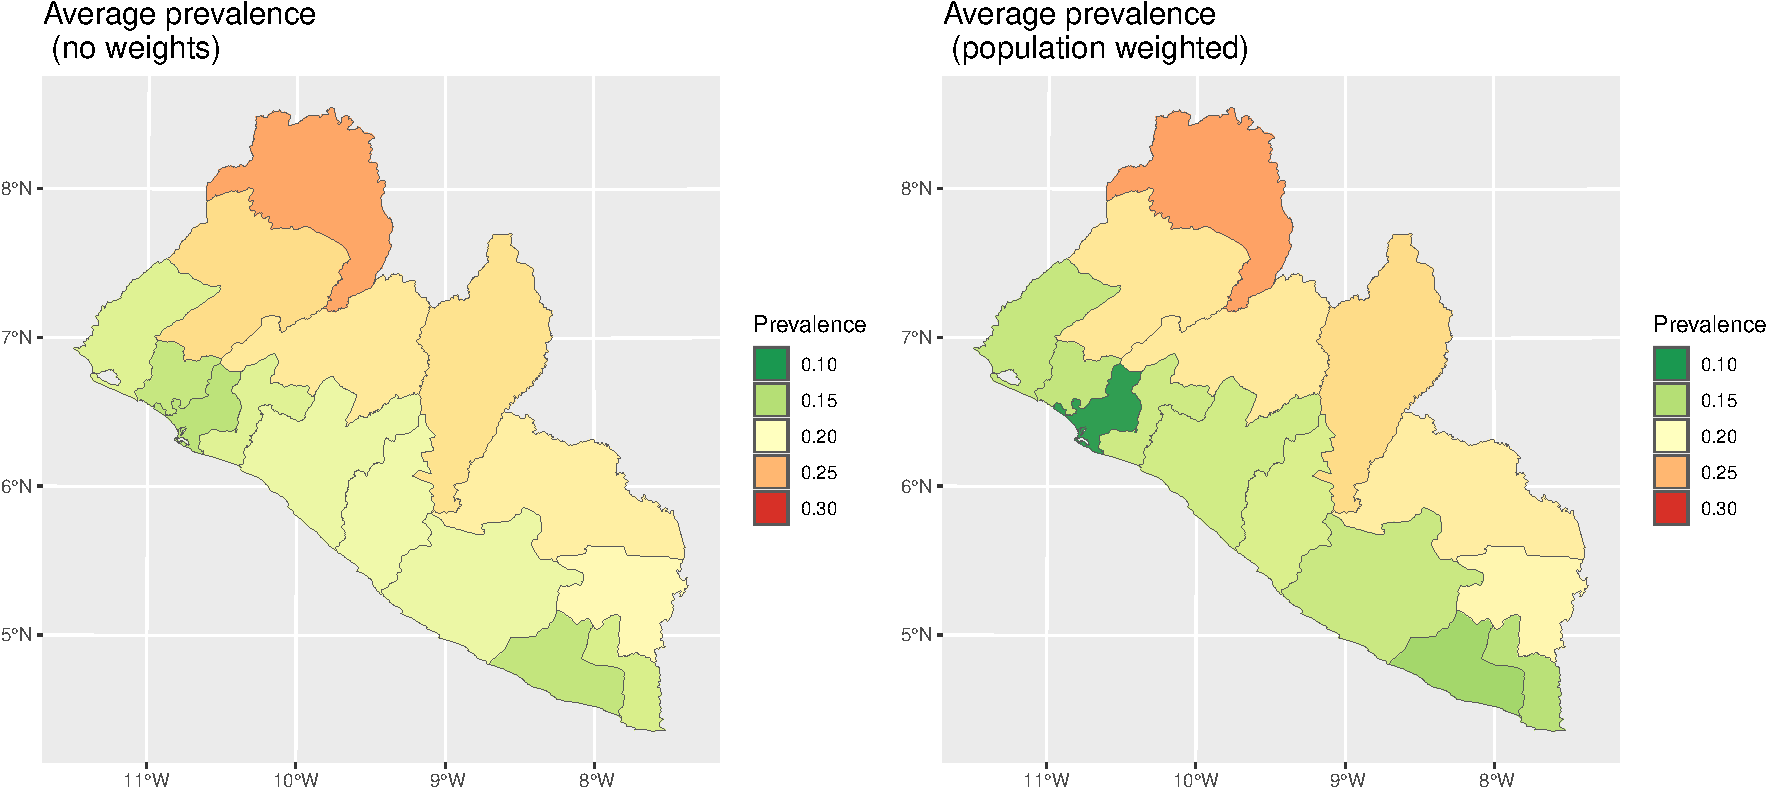
\includegraphics[keepaspectratio]{04_geostatistical-prediction_files/figure-pdf/fig-average-prev-Liberia-1.pdf}}

}

\caption{\label{fig-average-prev-Liberia}Maps of the predictive mean for
the admin level 1 average prevalence in Liberia. The left panel uses a
standard average of locations within an admin level 1 region, whilst in
the right panel each location is weighted according to population
density.}

\end{figure}%

In Figure~\ref{fig-average-prev-Liberia}, we observe that the
differences between the two predictive targets, with and without
weights, are not substantial. However, we observe that the predicted
average prevalence shows slightly greater variation in coastal regions,
particularly in Montserrado County, where the majority of the population
residing in the capital of Monrovia. This concentration of population
likely accounts for the more noticeable differences in this area.

\subsection{\texorpdfstring{Example: predicting the total number of
Anopheles gambiae mosquitoes (continuing from
Section~\ref{sec-anopheles-fit})}{Example: predicting the total number of Anopheles gambiae mosquitoes (continuing from Section~)}}\label{sec-anopheles-pred}

For the analysis on Anopheles gambiae mosquitoes, we consider the
prediction of the total number of mosquitoes within the study area. In
this case, because there is not a natural definition of the study area
borders as in the previous analysis, we consider the convex hull as
representing those borders. To pursue this let us first, visualize the
predictive map of the number of mosquitoes on a regular grid cover the
study area. In other words, we first consider the spatially continuous
target \[
T(x) = \exp\{\beta_0 + \beta_1 e(x) + S(x)\},
\] where, we recall, \(e(x)\) is the elevation in meters at location
\(x\). In the code below in addition to generate prediction for
\(T(x)\), we also create a binary indicator defined as \[
w(x) = 
\begin{cases}
1 & \text{if  } 390 < e(x) < 837 \\
0 & \text{otherwise.}
\end{cases}
\] The values of 390 and 837 meters correspond to the minimum and
maximum values of elevation observed in the data.

\begin{Shaded}
\begin{Highlighting}[]
\CommentTok{\# Create grid from convex hull}
\NormalTok{shp\_ch }\OtherTok{\textless{}{-}} \FunctionTok{convex\_hull\_sf}\NormalTok{(an\_fit}\SpecialCharTok{$}\NormalTok{data\_sf)}
\NormalTok{an\_grid }\OtherTok{\textless{}{-}} \FunctionTok{create\_grid}\NormalTok{(shp\_ch, }\AttributeTok{spat\_res =} \DecValTok{2}\NormalTok{)}


\NormalTok{an\_elev }\OtherTok{\textless{}{-}} \FunctionTok{get\_elev\_raster}\NormalTok{(}\AttributeTok{locations =}\NormalTok{ shp\_ch, }
                                \AttributeTok{z =} \DecValTok{9}\NormalTok{, }\AttributeTok{clip =} \StringTok{"locations"}\NormalTok{)}

\NormalTok{predictors }\OtherTok{\textless{}{-}} \FunctionTok{data.frame}\NormalTok{(}\AttributeTok{elevation=}\NormalTok{ terra}\SpecialCharTok{::}\FunctionTok{extract}\NormalTok{(an\_elev,}
                                                   \FunctionTok{st\_coordinates}\NormalTok{(an\_grid)))}

\NormalTok{pred\_an\_S }\OtherTok{\textless{}{-}} \FunctionTok{pred\_over\_grid}\NormalTok{(an\_fit, }\AttributeTok{grid =}\NormalTok{ an\_grid, }
               \AttributeTok{predictors =}\NormalTok{ predictors,}
               \AttributeTok{type =} \StringTok{"joint"}\NormalTok{)}

\NormalTok{pred\_n\_mosq\_grid }\OtherTok{\textless{}{-}} 
\FunctionTok{pred\_target\_grid}\NormalTok{(pred\_an\_S, }
                 \AttributeTok{f\_target =} \FunctionTok{list}\NormalTok{(}\AttributeTok{n\_mosq =} \ControlFlowTok{function}\NormalTok{(lp) }\FunctionTok{exp}\NormalTok{(lp)),}
                 \AttributeTok{pd\_summary =} \FunctionTok{list}\NormalTok{(}\AttributeTok{mean =} \ControlFlowTok{function}\NormalTok{(Tx) }\FunctionTok{mean}\NormalTok{(Tx)))}

\NormalTok{an\_weights }\OtherTok{\textless{}{-}} \DecValTok{1}\SpecialCharTok{*}\NormalTok{(predictors}\SpecialCharTok{$}\NormalTok{elevation }\SpecialCharTok{\textgreater{}} \DecValTok{390} \SpecialCharTok{\&}\NormalTok{ predictors}\SpecialCharTok{$}\NormalTok{elevation }\SpecialCharTok{\textless{}} \DecValTok{837}\NormalTok{)}
\end{Highlighting}
\end{Shaded}

We now define our predictive target corresponding to the total number of
mosquitoes within the study area \(A\), given by the convex hull of the
observed locations, as
\begin{equation}\phantomsection\label{eq-tot-mosq}{
T = \int_{A} w(x) T(x) \: dx
}\end{equation} The rationale is to estimate the total number of
mosquitoes in the study area while restricting predictions to locations
within the observed range of elevation. This approach helps avoid the
risk of predicting in ecological areas that may not be suitable for
mosquito presence. It is also important to note that in
Equation~\ref{eq-tot-mosq}, we do not standardize the weights in this
case.

\begin{Shaded}
\begin{Highlighting}[]
\FunctionTok{par}\NormalTok{(}\AttributeTok{mfrow =} \FunctionTok{c}\NormalTok{(}\DecValTok{1}\NormalTok{,}\DecValTok{2}\NormalTok{))}
\FunctionTok{plot}\NormalTok{(pred\_n\_mosq\_grid, }\AttributeTok{which\_target =} \StringTok{"n\_mosq"}\NormalTok{, }\AttributeTok{which\_summary =} \StringTok{"mean"}\NormalTok{,}
     \AttributeTok{main =} \StringTok{"Number of mosquitoes"}\NormalTok{)}
\FunctionTok{plot}\NormalTok{(an\_grid, }\AttributeTok{pch =} \DecValTok{20}\NormalTok{, }\AttributeTok{cex =} \DecValTok{1}\NormalTok{, }\AttributeTok{col =}\NormalTok{ an\_weights}\SpecialCharTok{+}\DecValTok{1}\NormalTok{, }\AttributeTok{main =} \StringTok{"Weights"}\NormalTok{)}
\FunctionTok{par}\NormalTok{(}\AttributeTok{mfrow =} \FunctionTok{c}\NormalTok{(}\DecValTok{1}\NormalTok{,}\DecValTok{1}\NormalTok{))}
\end{Highlighting}
\end{Shaded}

\begin{figure}[H]

\centering{

\pandocbounded{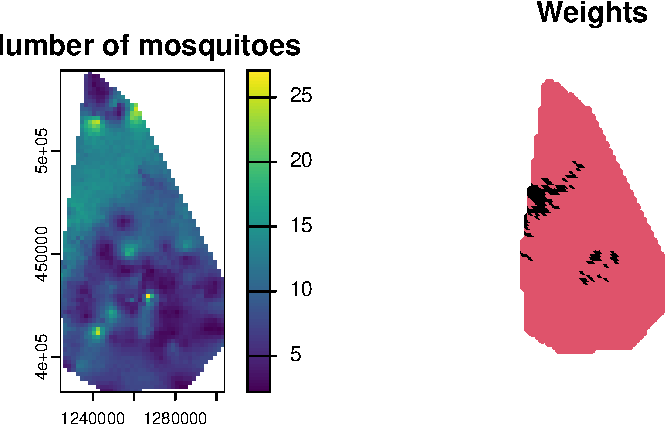
\includegraphics[keepaspectratio]{04_geostatistical-prediction_files/figure-pdf/fig-mosq-map-1.pdf}}

}

\caption{\label{fig-mosq-map}Maps of the predicted averae number of
mosqutoes (left panel). The right panel shows prediction locations in
red if they have an elevation between 390 and 837 meters, or black
otherwise.}

\end{figure}%

Figure~\ref{fig-mosq-map} shows the prediction map for the number of
mosquitoes at each prediction location, indicating a relatively high
spatial heterogeneity as was also indicated by the low value for the
estimate of the scale of the spatial correction (parameter \(\phi\)).
The right panel, we have an image of the weights \(w(x)\), with
locations that will not contribute to the prediction of the total number
of mosquitoes denoted in black.

\begin{Shaded}
\begin{Highlighting}[]
\NormalTok{pred\_n\_mosq\_shp }\OtherTok{\textless{}{-}} 
\FunctionTok{pred\_target\_shp}\NormalTok{(pred\_an\_S, }\AttributeTok{shp =}\NormalTok{ shp\_ch, }
                 \AttributeTok{weights =}\NormalTok{ an\_weights,}
                 \AttributeTok{shp\_target =}\NormalTok{ sum,}
                 \AttributeTok{f\_target =} \FunctionTok{list}\NormalTok{(}\AttributeTok{n\_mosq =} \ControlFlowTok{function}\NormalTok{(lp) }\FunctionTok{exp}\NormalTok{(lp)),}
                 \AttributeTok{pd\_summary =} \FunctionTok{list}\NormalTok{(}\AttributeTok{mean =} \ControlFlowTok{function}\NormalTok{(Tx) }\FunctionTok{mean}\NormalTok{(Tx),}
                                   \AttributeTok{q025 =} \ControlFlowTok{function}\NormalTok{(Tx) }\FunctionTok{quantile}\NormalTok{(Tx, }\FloatTok{0.025}\NormalTok{),}
                                   \AttributeTok{q075 =} \ControlFlowTok{function}\NormalTok{(Tx) }\FunctionTok{quantile}\NormalTok{(Tx, }\FloatTok{0.975}\NormalTok{)))}

\NormalTok{pred\_n\_mosq\_shp}\SpecialCharTok{$}\NormalTok{target}\SpecialCharTok{$}\NormalTok{reg1}\SpecialCharTok{$}\NormalTok{n\_mosq}
\DocumentationTok{\#\# $mean}
\DocumentationTok{\#\# [1] 19525.46}
\DocumentationTok{\#\# }
\DocumentationTok{\#\# $q025}
\DocumentationTok{\#\#     2.5\% }
\DocumentationTok{\#\# 16306.64 }
\DocumentationTok{\#\# }
\DocumentationTok{\#\# $q075}
\DocumentationTok{\#\#    97.5\% }
\DocumentationTok{\#\# 23452.84}
\end{Highlighting}
\end{Shaded}

Since we are not standardizing the weights, there is no need to specify
\texttt{standardize\_weights}, as it is set to \texttt{FALSE} by
default. In the code above, we printed the mean of the predictive
distribution of \(T\) along with the 95\% prediction interval. The point
estimate of approximately 17,719 mosquitoes is likely an underestimate
of the total number of Anopheles gambiae in the area, as the trap used
to count the mosquitoes may not capture all of them, particularly those
outside the immediate trapping zone or those active at different times.

\section{Assessing the predictive performance of geostatistical models
with cross-validation}\label{sec-compare-pp}

In this section, we address the problem of identifying the
geostatistical model that offers the best predictive performance among a
set of candidates. However, we first need a clear definition of
predictive performance which can be used to select suitable statistical
tools that can be to used to evaluate it. Broadly speaking, predictive
performance is defined by how well a model's predictive distribution
aligns with observed data. Evaluating predictive performance requires
examining two key characteristics of the predictive distribution:
\emph{sharpness} and \emph{calibration}.

\subsection{How to split geostatistical data for model performance
comparisons}\label{sec-split-data}

To carry out the assessment and comparison of the predictive performance
of geostatistical models using the methods illustrated in the following
sections, the first crucial step is to decide which approach to use to
split the data-set into a \emph{training set} and \emph{test set}. In
the context of geostatistical analysis, the \emph{training set} is the
subset of the original data-set that is used to estimate the model
parameters and then predict at the locations of the \emph{test set},
which is used to assess how well the model can predict unseen data.

When splitting geostatistical data-sets for model performance
evaluation, it is essential to consider the objective of the spatial
prediction. Here, we consider two main prediction objectives: 1)
predicting in areas disjoint from the study area where there are no
data; 2) inferring the spatial surface of disease risk within a given
study area. Let us give an example to better explain the difference
between these two objectives. Under objective 1), if survey data exist
for a specific country, say Kenya, but not for a neighboring country,
say Somalia, a model trained on Kenyan data might then be used to
predict disease prevalence in Somalia. In objective 2), instead,
high-resolution risk maps of a health outcome might be required within a
single country. The splitting of geostatistical data for predictive
performance assessment should align with the intended application of the
model and reflect whether the goal is to predict in entirely disjoint
areas with no data (objective 1) or to infer the spatial surface of
interest within the same study area (objective 2). Below, we elaborate
on suitable methods for each of these two.

In the first scenario (objective 1) ), splitting the data using k-fold
cross-validation with spatially coherent folds is more appropriate.
These folds can be created using clustering methods such as k-means or
hierarchical clustering (see Yin et al. (2024) for review of the main
clustering methods). These methods group spatial locations based on
their coordinates or covariates, ensuring each fold represents a
distinct spatial region. This approach mimics the challenge of
predicting in disjoint areas by withholding entire spatial clusters from
the training data. For instance, k-means minimizes within-cluster
variance to produce compact, non-overlapping groups, while hierarchical
clustering organizes data into nested clusters based on a linkage
criterion like geographic distance. In the code below we show an example
of the use of these methods for data splitting, using the
\texttt{spatial\_clusterin\_cv} function from the \texttt{spatialsample}
package (Mahoney et al. 2023).

\begin{Shaded}
\begin{Highlighting}[]
\FunctionTok{library}\NormalTok{(spatialsample)}
\FunctionTok{set.seed}\NormalTok{(}\DecValTok{123}\NormalTok{)}
\NormalTok{liberia\_sf }\OtherTok{\textless{}{-}}\NormalTok{ liberia }\SpecialCharTok{\%\textgreater{}\%}
              \FunctionTok{st\_as\_sf}\NormalTok{(., }\AttributeTok{coords =} \FunctionTok{c}\NormalTok{(}\StringTok{"long"}\NormalTok{, }\StringTok{"lat"}\NormalTok{),}
                       \AttributeTok{crs =} \DecValTok{4326}\NormalTok{) }\SpecialCharTok{\%\textgreater{}\%}
              \FunctionTok{st\_transform}\NormalTok{(.,}\AttributeTok{crs =} \DecValTok{32629}\NormalTok{)}


\CommentTok{\# K{-}means}
\NormalTok{kmeans\_liberia }\OtherTok{\textless{}{-}} \FunctionTok{spatial\_clustering\_cv}\NormalTok{(liberia\_sf,}
                      \AttributeTok{v =} \DecValTok{10}\NormalTok{, }\AttributeTok{cluster\_function =} \StringTok{"kmeans"}\NormalTok{)}
\NormalTok{kmeans\_plot }\OtherTok{\textless{}{-}} \FunctionTok{autoplot}\NormalTok{(kmeans\_liberia) }\SpecialCharTok{+} \FunctionTok{ggtitle}\NormalTok{(}\StringTok{"K{-}means"}\NormalTok{)}

\CommentTok{\# Hierarchical clustering}
\NormalTok{hclust\_liberia }\OtherTok{\textless{}{-}} \FunctionTok{spatial\_clustering\_cv}\NormalTok{(liberia\_sf,}
                      \AttributeTok{v =} \DecValTok{10}\NormalTok{, }\AttributeTok{cluster\_function =} \StringTok{"hclust"}\NormalTok{) }
                   

\NormalTok{hclust\_plot }\OtherTok{\textless{}{-}} \FunctionTok{autoplot}\NormalTok{(hclust\_liberia) }\SpecialCharTok{+}
  \FunctionTok{ggtitle}\NormalTok{(}\StringTok{"Hierarchical clustering"}\NormalTok{)}

\FunctionTok{library}\NormalTok{(gridExtra)}
\FunctionTok{grid.arrange}\NormalTok{(kmeans\_plot, hclust\_plot, }\AttributeTok{ncol =} \DecValTok{2}\NormalTok{)}
\end{Highlighting}
\end{Shaded}

\begin{figure}[H]

\centering{

\pandocbounded{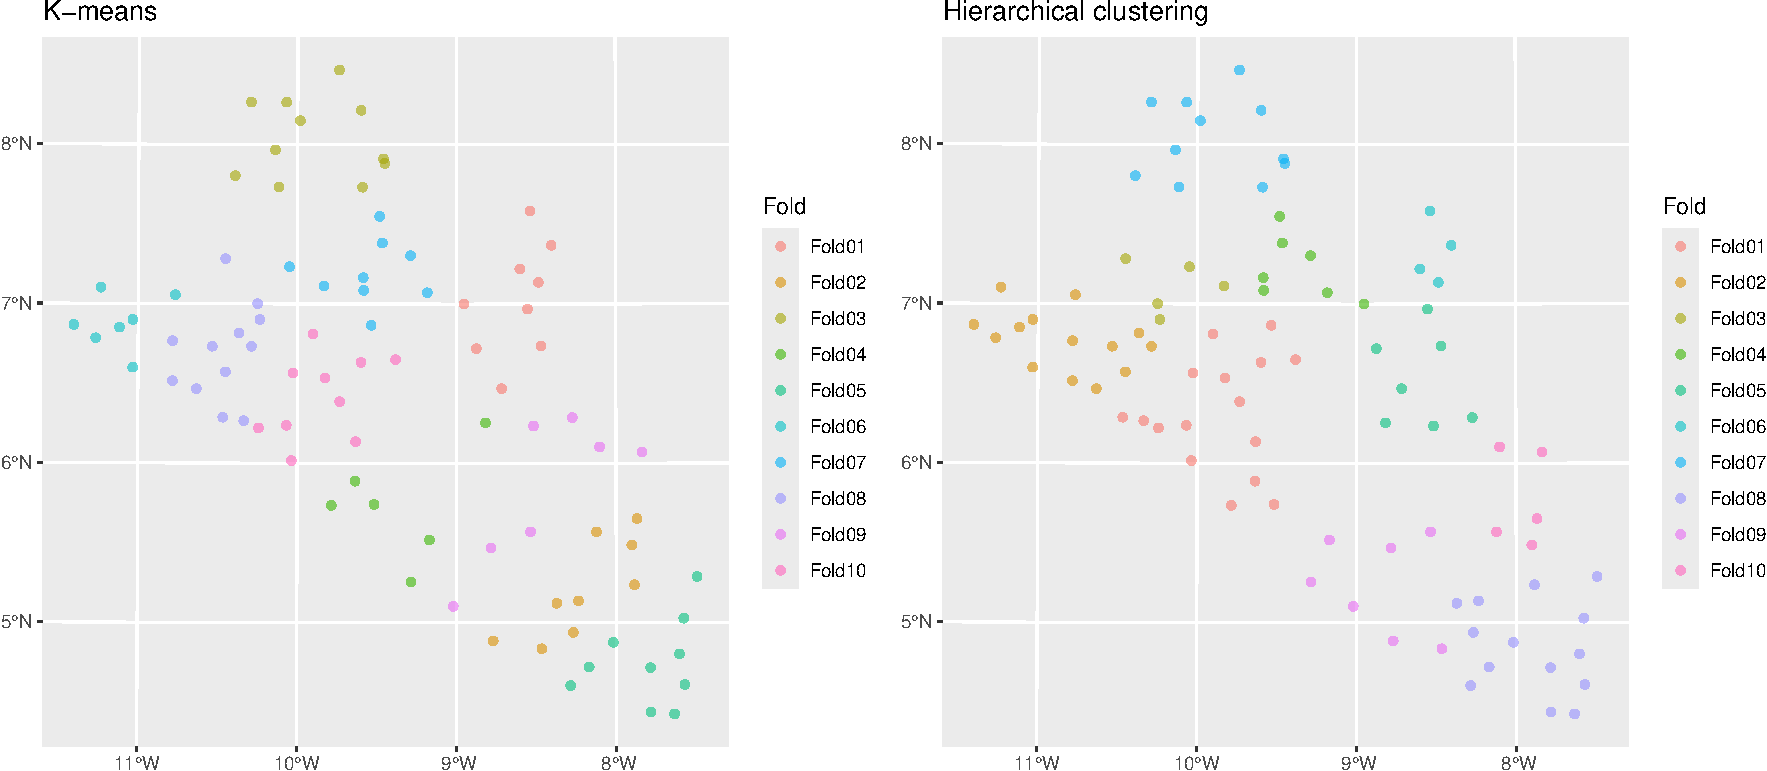
\includegraphics[keepaspectratio]{04_geostatistical-prediction_files/figure-pdf/fig-clus-loc-1.pdf}}

}

\caption{\label{fig-clus-loc}Examples un the use of spatial clustering
methods for the splitting of the Liberia data on riverblindness.}

\end{figure}%

The results of the splitting are shown in Figure~\ref{fig-clus-loc},
where we have generated 10 folds using the k-means and hierarchical
clustering methods with the default options. We can observe that the
test sets are very similar, with fold 3 from the k-means and fold 7 from
hierarchical clustering being identical. If using only the distance
between locations to cluster the data into different folds, the choice
of clustering method should have much impact on the model assessment as
long as we repeat the split and assessment of the methods multiple times
as we will show later in the next sections.

Before proceeding further, it is important to highlight that when the
objective is predicting an outcome in entirely disjoint areas, the risks
and limitations of this assessment should be carefully considered. In
such cases, predictions are predominantly driven by covariates because
the spatial Gaussian process \(S(x)\) cannot extrapolate spatial
patterns across regions with no connecting data. When the disjoint
region requiring predictions is far from the sampled data, the Gaussian
process contributes primarily to inflating prediction uncertainty and
has no tangible impact on the point predictions, reflecting the lack of
ground data in the area. Consequently, this validation approach
primarily assesses the predictive power of the covariates rather than
the geostatistical model as a whole. This limitation may lead to
overestimating the model's generalization capabilities, especially if
the model is being used to predict areas that are far away from the
study area. Hence, the results of this validation should be interpreted
cautiously, emphasizing the critical role of covariates in driving
predictions under such conditions.

We now consider the second prediction objective of inferring the spatial
surface within the study area. In this case, a random sampling approach
can be employed. However, to preserve a good spatial coverage of the
study area, a minimum distance can be imposed between selected
locations. For example, methods such as spatial thinning or stratified
sampling can be adapted to enforce a minimum spatial separation. This
can be done in R using the \texttt{subsample.distance} function from the
\texttt{spatialEco} package (Evans and Murphy 2021).

\begin{Shaded}
\begin{Highlighting}[]
\FunctionTok{library}\NormalTok{(spatialEco)}
\FunctionTok{set.seed}\NormalTok{(}\DecValTok{123}\NormalTok{)}

\CommentTok{\# Regulirized spatial sampling: 30km}
\NormalTok{dist30\_liberia }\OtherTok{\textless{}{-}} \FunctionTok{subsample.distance}\NormalTok{(liberia\_sf,}
                      \AttributeTok{size =} \DecValTok{20}\NormalTok{, }\AttributeTok{d =} \DecValTok{30000}\NormalTok{)}
\NormalTok{dist30\_plot }\OtherTok{\textless{}{-}} \FunctionTok{ggplot}\NormalTok{(dist30\_liberia) }\SpecialCharTok{+} \FunctionTok{geom\_sf}\NormalTok{() }\SpecialCharTok{+}
               \FunctionTok{theme\_minimal}\NormalTok{() }\SpecialCharTok{+} 
               \FunctionTok{ggtitle}\NormalTok{(}\StringTok{"Minimum distance: 30km"}\NormalTok{)}

\CommentTok{\# Regulirized spatial sampling: 40km}
\NormalTok{dist40\_liberia }\OtherTok{\textless{}{-}} \FunctionTok{subsample.distance}\NormalTok{(liberia\_sf,}
                      \AttributeTok{size =} \DecValTok{20}\NormalTok{, }\AttributeTok{d =} \DecValTok{40000}\NormalTok{)}
\NormalTok{dist40\_plot }\OtherTok{\textless{}{-}} \FunctionTok{ggplot}\NormalTok{(dist40\_liberia) }\SpecialCharTok{+} \FunctionTok{geom\_sf}\NormalTok{() }\SpecialCharTok{+}
               \FunctionTok{theme\_minimal}\NormalTok{() }\SpecialCharTok{+} 
               \FunctionTok{ggtitle}\NormalTok{(}\StringTok{"Minimum distance: 40km"}\NormalTok{)}

\FunctionTok{grid.arrange}\NormalTok{(dist30\_plot, dist40\_plot, }\AttributeTok{ncol =} \DecValTok{2}\NormalTok{)}
\end{Highlighting}
\end{Shaded}

\begin{figure}[H]

\centering{

\pandocbounded{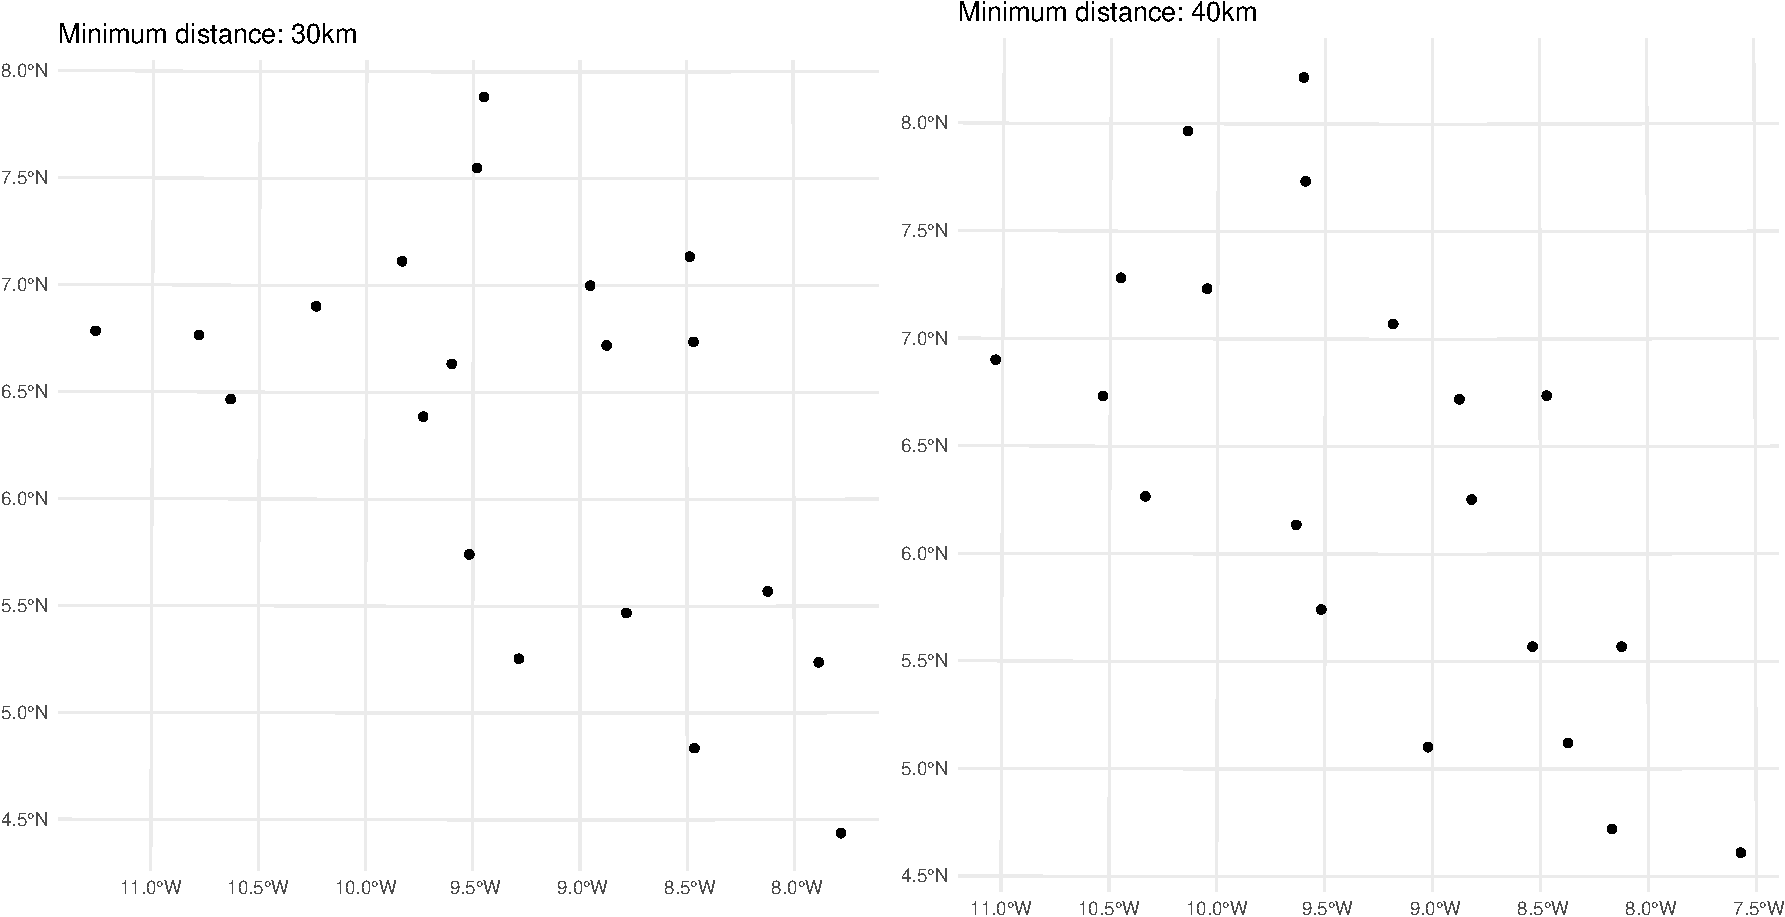
\includegraphics[keepaspectratio]{04_geostatistical-prediction_files/figure-pdf/fig-reg-loc-1.pdf}}

}

\caption{\label{fig-reg-loc}Examples un the use of spatialky regularized
thinning for the splitting of the Liberia data on riverblindness into
training and test set. The plots show the resulting test sets by
randomly selecting 20 locations from the original data-set and imposing
a minimum distance of 30km (left panel) and 40km (right panel).}

\end{figure}%

In the code above, we randomly selected 20 locations from the original
data-set, enforcing minimum distances of 30 km and 40 km between points.
The results are presented in Figure~\ref{fig-reg-loc}. The choice of the
minimum distance for the test sample should ideally consider the spatial
correlation scale (previously denoted by \(\phi\)) of the spatial
Gaussian process \(S(X)\). To minimize correlation within the test set,
the minimum distance could be set to a value greater than \(\phi\).
However, increasing the minimum distance makes it more challenging to
obtain a test set of the desired sample size. Reducing correlation
within the test set is important for ensuring that the assessment of
predictive performance is as robust as possible.

A key challenge in both approaches is the potential lack of independence
between the training and test data-sets due to spatial correlation. This
can lead to an overly optimistic evaluation of model performance, as the
training set may already contain information that is correlated with the
test set. However, if we assume that all models benefit equally from
this correlation during performance evaluation, the methods we
illustrate next can still provide a reliable comparison of model
performance in relative terms, even if the considered performance
metrics may be somewhat biased.

\subsection{Assessing calibration using the nonrandomized probability
integral transform}\label{sec-anpit}

A model is considered \emph{well-calibrated} if its predictions
adequately reflect the true uncertainty of the data. Assessment of a
model's calibration can be carried out in several ways. We can examine
the agreement between the point predictions, say \(\hat{y}_i\), and the
observed outcomes \(y_i\), commonly referred to as \emph{accuracy}. The
mean squared error (MSE), defined as
\(\text{MSE} = \frac{1}{n} \sum_{i=1}^n (y_i - \hat{y}_i)^2\), is an
example of a commonly used metric to evaluate the accuracy of a model.
To characterize calibration more fully, it is also essential to quantify
the spread of the predictive distributions, which also defines the
\emph{precision} of predictions. For example, prediction intervals
generated from the predictive distribution for \(y_i\) can help assess
the precision of a geostatistical model. In summary, a well-calibrated
model is both accurate and precise.

Assessment of the calibration of the model should precede the assessment
of sharpness, since, as we shall see in the next section, this relies on
the model being well-calibrated. The probability integral transform
(PIT) was originally proposed by Dawid (1984) as a way to assess the
calibration of a model. The PIT is based on the simple observation that
if we consider a variable \(Y\) and apply the transformation
\(Y^* = F_{Y}(Y)\), where \(F_{Y}(\cdot)\) is the cumulative density
function (or cumulative distribution if \(Y\) is discrete) of \(Y\), it
then follows that \(Y^*\) follows a uniform distribution in the unit
interval. The fundamental problem and the reason why statistical
modelling exists is that we do not \(F_{Y}\) but we would like to
propose a model \(M\) that we believe adequately approximates \(F_{Y}\)
with \(F_{M}\). The main advantage of using the PIT is that assessment
of whether \(M\) is well calibrated reduces to assessing whether the
transform set of data \(F_{M}(y_1), \ldots, F_{M}(y_n)\) follows a
uniform distribution. To illustrate this, let us a consider a simple
simulated example.

We first create a function that can compute the PIT.

\begin{Shaded}
\begin{Highlighting}[]
\CommentTok{\# Define a function for the PIT}
\CommentTok{\# F\_M is the cumulative density function generated by the adopted model}
\NormalTok{pit\_transform }\OtherTok{\textless{}{-}} \ControlFlowTok{function}\NormalTok{(data, F\_M) \{}
  \CommentTok{\# Apply the model CDF to the data}
\NormalTok{  pit\_values }\OtherTok{\textless{}{-}} \FunctionTok{F\_M}\NormalTok{(data)}
  \FunctionTok{return}\NormalTok{(pit\_values)}
\NormalTok{\}}
\end{Highlighting}
\end{Shaded}

We then apply this function to show how the assessment of calibration
through the PIT is carried out under two scenarios: 1) \(F_{Y}\) is a
Gamma distribution with shape 2 and scale parameter 1; 2) \(F_{Y}\) is
Student's T distribution with 3 degrees of freedom. In each of the two
scenarios, we show how the PIT behaves when our model coincides with the
the true model (i.e.~\(F_{M} = F_{Y}\)) and when instead our model \(M\)
is a Gaussian distribution, with mean and variance estimated from the
data.

\begin{Shaded}
\begin{Highlighting}[]
\CommentTok{\# Generate data from a skewed (gamma) distribution}
\NormalTok{n }\OtherTok{\textless{}{-}} \DecValTok{1000}
\NormalTok{shape }\OtherTok{\textless{}{-}} \DecValTok{2}
\NormalTok{rate }\OtherTok{\textless{}{-}} \DecValTok{1}
\NormalTok{data\_gamma }\OtherTok{\textless{}{-}} \FunctionTok{rgamma}\NormalTok{(n, }\AttributeTok{shape =}\NormalTok{ shape, }\AttributeTok{rate =}\NormalTok{ rate)}

\CommentTok{\# Define correct and incorrect model CDFs for gamma data}
\CommentTok{\# Correct CDF}
\NormalTok{model\_cdf\_correct\_gamma }\OtherTok{\textless{}{-}} \ControlFlowTok{function}\NormalTok{(x) }\FunctionTok{pgamma}\NormalTok{(x, }\AttributeTok{shape =}\NormalTok{ shape, }\AttributeTok{rate =}\NormalTok{ rate)}
\CommentTok{\# Incorrect CDF: Assume data is normal (wrong model)}
\NormalTok{model\_cdf\_incorrect\_gamma }\OtherTok{\textless{}{-}} \ControlFlowTok{function}\NormalTok{(x) }\FunctionTok{pnorm}\NormalTok{(x, }\AttributeTok{mean =} \FunctionTok{mean}\NormalTok{(data\_gamma), }\AttributeTok{sd =} \FunctionTok{sd}\NormalTok{(data\_gamma))}

\CommentTok{\# Compute PIT values for gamma data under both models}
\NormalTok{pit\_correct\_gamma }\OtherTok{\textless{}{-}} \FunctionTok{pit\_transform}\NormalTok{(data\_gamma, model\_cdf\_correct\_gamma)}
\NormalTok{pit\_incorrect\_gamma }\OtherTok{\textless{}{-}} \FunctionTok{pit\_transform}\NormalTok{(data\_gamma, model\_cdf\_incorrect\_gamma)}

\CommentTok{\# Generate data from a heavy{-}tailed (t) distribution}
\NormalTok{df }\OtherTok{\textless{}{-}} \DecValTok{3}
\NormalTok{data\_t }\OtherTok{\textless{}{-}} \FunctionTok{rt}\NormalTok{(n, }\AttributeTok{df =}\NormalTok{ df)}

\CommentTok{\# Define correct and incorrect model CDFs for t data}
\CommentTok{\# Correct CDF}
\NormalTok{model\_cdf\_correct\_t }\OtherTok{\textless{}{-}} \ControlFlowTok{function}\NormalTok{(x) }\FunctionTok{pt}\NormalTok{(x, }\AttributeTok{df =}\NormalTok{ df)}
\CommentTok{\# Incorrect CDF: Assume data is normal (wrong model)}
\NormalTok{model\_cdf\_incorrect\_t }\OtherTok{\textless{}{-}} \ControlFlowTok{function}\NormalTok{(x) }\FunctionTok{pnorm}\NormalTok{(x, }\AttributeTok{mean =} \FunctionTok{mean}\NormalTok{(data\_t), }\AttributeTok{sd =} \FunctionTok{sd}\NormalTok{(data\_t))}

\CommentTok{\# Compute PIT values for t data under both models}
\NormalTok{pit\_correct\_t }\OtherTok{\textless{}{-}} \FunctionTok{pit\_transform}\NormalTok{(data\_t, model\_cdf\_correct\_t)}
\NormalTok{pit\_incorrect\_t }\OtherTok{\textless{}{-}} \FunctionTok{pit\_transform}\NormalTok{(data\_t, model\_cdf\_incorrect\_t)}

\CommentTok{\# Combine results into a data frame for plotting}
\NormalTok{df\_plot }\OtherTok{\textless{}{-}} \FunctionTok{data.frame}\NormalTok{(}
  \AttributeTok{PIT =} \FunctionTok{c}\NormalTok{(pit\_correct\_gamma, pit\_incorrect\_gamma, pit\_correct\_t, pit\_incorrect\_t),}
  \AttributeTok{Model =} \FunctionTok{rep}\NormalTok{(}\FunctionTok{c}\NormalTok{(}\StringTok{"Correct Gamma Model"}\NormalTok{, }\StringTok{"Incorrect Normal Model for Gamma"}\NormalTok{, }
                \StringTok{"Correct t Model"}\NormalTok{, }\StringTok{"Incorrect Normal Model for t"}\NormalTok{), }\AttributeTok{each =}\NormalTok{ n)}
\NormalTok{)}

\CommentTok{\# Plot PIT distributions}
\NormalTok{hist\_plot }\OtherTok{\textless{}{-}} \FunctionTok{ggplot}\NormalTok{(df\_plot, }\FunctionTok{aes}\NormalTok{(}\AttributeTok{x =}\NormalTok{ PIT)) }\SpecialCharTok{+}
  \FunctionTok{geom\_histogram}\NormalTok{(}\FunctionTok{aes}\NormalTok{(}\AttributeTok{y =}\NormalTok{ ..density..), }\AttributeTok{bins =} \DecValTok{20}\NormalTok{, }\AttributeTok{fill =} \StringTok{"skyblue"}\NormalTok{, }\AttributeTok{color =} \StringTok{"black"}\NormalTok{, }\AttributeTok{alpha =} \FloatTok{0.7}\NormalTok{) }\SpecialCharTok{+}
  \FunctionTok{geom\_hline}\NormalTok{(}\AttributeTok{yintercept =} \DecValTok{1}\NormalTok{, }\AttributeTok{linetype =} \StringTok{"dashed"}\NormalTok{, }\AttributeTok{color =} \StringTok{"red"}\NormalTok{) }\SpecialCharTok{+}
  \FunctionTok{facet\_wrap}\NormalTok{(}\SpecialCharTok{\textasciitilde{}}\NormalTok{ Model, }\AttributeTok{scales =} \StringTok{"free"}\NormalTok{) }\SpecialCharTok{+}
  \FunctionTok{labs}\NormalTok{(}\AttributeTok{title =} \StringTok{"Probability Integral Transform (PIT) Distributions"}\NormalTok{,}
       \AttributeTok{x =} \StringTok{"PIT Values"}\NormalTok{,}
       \AttributeTok{y =} \StringTok{"Density"}\NormalTok{) }\SpecialCharTok{+}
  \FunctionTok{theme\_minimal}\NormalTok{()}

\CommentTok{\# Display the plot}
\FunctionTok{print}\NormalTok{(hist\_plot)}
\end{Highlighting}
\end{Shaded}

\begin{figure}[H]

\centering{

\pandocbounded{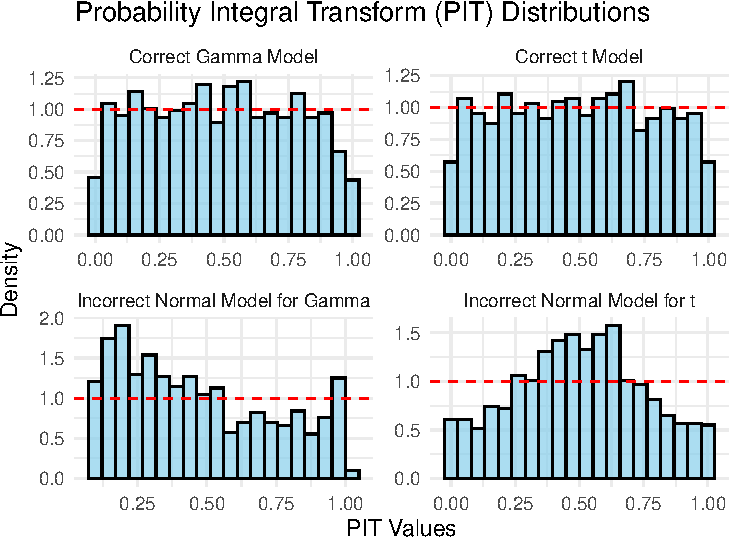
\includegraphics[keepaspectratio]{04_geostatistical-prediction_files/figure-pdf/fig-hist-pit-1.pdf}}

}

\caption{\label{fig-hist-pit}Histograms of the probability integral
transform applied to simulated data. The top panels show the histograma
of the PIT when the fitted model coincides with the true data generating
model. The lower panels show how the PIT histrograms deviate from a
uniform distribution. For more details, we refer to main text.}

\end{figure}%

In Figure~\ref{fig-hist-pit}, we assess whether the PIT transformed data
follow a uniform distribution if the bars of the histogram are all
approximately at the same height as indicated by the dashed line. Our
preference to this diagnostic plot, is to use a qq-plot for a uniform
distribution as shown below.

\begin{Shaded}
\begin{Highlighting}[]
\CommentTok{\# QQ plot to check uniformity of PIT values}
\NormalTok{qq\_plot }\OtherTok{\textless{}{-}} \FunctionTok{ggplot}\NormalTok{(df\_plot, }\FunctionTok{aes}\NormalTok{(}\AttributeTok{sample =}\NormalTok{ PIT)) }\SpecialCharTok{+}
  \FunctionTok{stat\_qq}\NormalTok{(}\AttributeTok{distribution =}\NormalTok{ qunif) }\SpecialCharTok{+}
  \FunctionTok{stat\_qq\_line}\NormalTok{(}\AttributeTok{distribution =}\NormalTok{ qunif, }\AttributeTok{color =} \StringTok{"red"}\NormalTok{) }\SpecialCharTok{+}
  \FunctionTok{facet\_wrap}\NormalTok{(}\SpecialCharTok{\textasciitilde{}}\NormalTok{ Model, }\AttributeTok{scales =} \StringTok{"free"}\NormalTok{) }\SpecialCharTok{+}
  \FunctionTok{labs}\NormalTok{(}\AttributeTok{title =} \StringTok{"QQ Plot of PIT Values against Uniform Distribution"}\NormalTok{,}
       \AttributeTok{x =} \StringTok{"Theoretical Quantiles (Uniform)"}\NormalTok{,}
       \AttributeTok{y =} \StringTok{"Sample Quantiles (PIT Values)"}\NormalTok{) }\SpecialCharTok{+}
  \FunctionTok{theme\_minimal}\NormalTok{()}

\CommentTok{\# Display both plot}
\FunctionTok{print}\NormalTok{(qq\_plot)}
\end{Highlighting}
\end{Shaded}

\begin{figure}[H]

\centering{

\pandocbounded{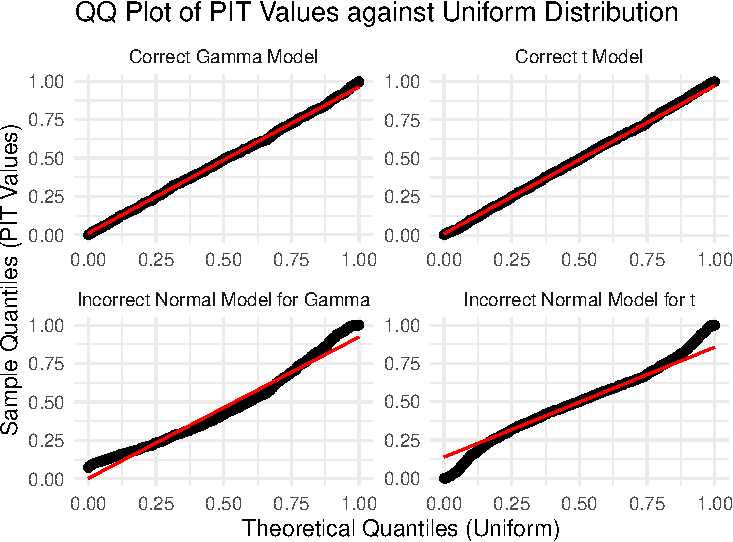
\includegraphics[keepaspectratio]{04_geostatistical-prediction_files/figure-pdf/fig-qqplot-pit-1.pdf}}

}

\caption{\label{fig-qqplot-pit}QQ-plots of the probability integral
transform applied to simulated data. The top panels show the histograma
of the PIT when the fitted model coincides with the true data generating
model. The lower panels show how the PIT qq-plots deviate from a uniform
distribution. The red line is the identity line For more details, we
refer to main text.}

\end{figure}%

In the results of Figure~\ref{fig-qqplot-pit}, we consider a model
well-calibrated if the qq-plot is as close as possible to the identity
line. It is clear that in the first case the use of Gaussian
distribution is violated by the skewness of the data generated from a
Gamma distribution, and in the second scenario by the heavier tail of
the Student's T distribution.

In the simulated example, the PIT might seem unnecessary because we can
directly assess if the data follow the assumed distribution (Gamma,
Gaussian, or Student's T) by comparing empirical and theoretical
distributions. In these simple models, including linear Gaussian
geostatistical models, the marginal distribution of the data is
analytically available, so assessing goodness-of-fit is straightforward.

However, in the case of Binomial and Poisson geostatistical models, the
marginal distribution of the data \(Y\) -- unconditioned on the spatial
random effects \(S(x)\) -- cannot be obtained analytically.
Specifically, geostatistical models for count data assume that \(Y\),
conditioned on \(S(x)\), follows either a Binomial or Poisson
distribution. But once we integrate out \(S(x)\) to obtain the marginal
(i.e., unconditioned) distribution of \(Y\), this distribution is no
longer Poisson or Binomial. Instead, it becomes an overdispersed count
distribution that lacks a closed-form expression.

In such cases, the PIT becomes valuable for evaluating model adequacy,
as it allows for assessing the uniformity of PIT values against the
assumed model distribution, even when the marginal distribution is
intractable. However, direct application of the PIT raises the issue
that the the transformation \(F_{Y}(Y)\) does not follow a uniform
distribution, because of the discrete nature of the random variable
\(Y\). Hence, for a given discrete-outcome model \(M\), we use a
modified version of the PIT, referred to as nonrandomized PIT
(henceforth, nPIT), originally proposed by Czado, Gneiting, and Held
(2009), taking the form \begin{equation}\phantomsection\label{eq-anpit}{
\text{nPIT}(u,y) = 
\begin{cases} 
0, & u \leq F_{M}(y-1) \\ 
\frac{u - F_{M}(y-1)}{F_{M}(y-1) - F_{M}(y-1)}, & F_{M}(y-1) \leq u \leq F_{M}(y) \\ 
1, & u \geq F_{M}(y)
\end{cases}.
}\end{equation} We then take the average nPIT over the observed outcomes
\(y_{1}, \ldots, y_{n}\), hence \[
\text{AnPIT}(u) = \frac{1}{n} \sum_{i=1}^n \text{nPIT}(u, y_{i}). 
\] Assessment of calibration is then carried out by checking wether the
AnPIT is as close as possible to the identity function,
i.e.~\(\text{AnPIT}(u) = u\). Hence, by plotting \(\text{AnPIT}(u)\)
against \(u\), we can consider any deviations from the identity line as
evidence that the model is not well-calibrated.

We now illustrate the use of the AnPIT through a simulated example. We
simulate data from a negative Binomial distribution, with mean
\(\lambda = 5\) and dispersion parameter \(\alpha = 1/2\), hence
\(E[Y] = \lambda\) and
\(\text{Var}[Y] = \lambda \times (1 + \alpha \lambda)\).

\begin{Shaded}
\begin{Highlighting}[]
\CommentTok{\# Parameters for the Negative Binomial distribution}
\FunctionTok{set.seed}\NormalTok{(}\DecValTok{123}\NormalTok{)}
\NormalTok{n }\OtherTok{\textless{}{-}} \DecValTok{200}                \CommentTok{\# number of simulations}
\NormalTok{lambda }\OtherTok{\textless{}{-}} \DecValTok{5}             \CommentTok{\# mean}
\NormalTok{dispersion }\OtherTok{\textless{}{-}} \FloatTok{0.5}       \CommentTok{\# dispersion parameter}
\NormalTok{size }\OtherTok{\textless{}{-}} \DecValTok{1} \SpecialCharTok{/}\NormalTok{ dispersion  }\CommentTok{\# size parameter for negative binomial}

\CommentTok{\# Simulate data from the Negative Binomial distribution}
\NormalTok{sim\_data\_nb }\OtherTok{\textless{}{-}} \FunctionTok{rnbinom}\NormalTok{(n, }\AttributeTok{size =}\NormalTok{ size, }\AttributeTok{mu =}\NormalTok{ lambda)}

\CommentTok{\# Define the nonrandomized PIT function}
\NormalTok{compute\_npit }\OtherTok{\textless{}{-}} \ControlFlowTok{function}\NormalTok{(y, u, cdf\_func) \{}
  \CommentTok{\# Calculate cumulative probabilities F\_M(y{-}1) and F\_M(y) using the provided CDF function}
\NormalTok{  f\_y\_minus\_1 }\OtherTok{\textless{}{-}} \FunctionTok{cdf\_func}\NormalTok{(y }\SpecialCharTok{{-}} \DecValTok{1}\NormalTok{)}
\NormalTok{  f\_y }\OtherTok{\textless{}{-}} \FunctionTok{cdf\_func}\NormalTok{(y)}
  
  \CommentTok{\# Apply the piecewise formula for nPIT}
  \ControlFlowTok{if}\NormalTok{ (u }\SpecialCharTok{\textless{}=}\NormalTok{ f\_y\_minus\_1) \{}
    \FunctionTok{return}\NormalTok{(}\DecValTok{0}\NormalTok{)}
\NormalTok{  \} }\ControlFlowTok{else} \ControlFlowTok{if}\NormalTok{ (u }\SpecialCharTok{\textless{}=}\NormalTok{ f\_y) \{}
    \FunctionTok{return}\NormalTok{((u }\SpecialCharTok{{-}}\NormalTok{ f\_y\_minus\_1) }\SpecialCharTok{/}\NormalTok{ (f\_y }\SpecialCharTok{{-}}\NormalTok{ f\_y\_minus\_1))}
\NormalTok{  \} }\ControlFlowTok{else}\NormalTok{ \{}
    \FunctionTok{return}\NormalTok{(}\DecValTok{1}\NormalTok{)}
\NormalTok{  \}}
\NormalTok{\}}

\CommentTok{\# Generate a sequence of u values from 0 to 1}
\NormalTok{u\_values }\OtherTok{\textless{}{-}} \FunctionTok{seq}\NormalTok{(}\DecValTok{0}\NormalTok{, }\DecValTok{1}\NormalTok{, }\AttributeTok{length.out =} \DecValTok{100}\NormalTok{)}

\CommentTok{\# Calculate the average nPIT for each u value for both models}
\NormalTok{AnPIT\_nb }\OtherTok{\textless{}{-}} \FunctionTok{sapply}\NormalTok{(u\_values, }\ControlFlowTok{function}\NormalTok{(u) \{}
  \FunctionTok{mean}\NormalTok{(}\FunctionTok{sapply}\NormalTok{(sim\_data\_nb, compute\_npit, }\AttributeTok{u =}\NormalTok{ u, }\AttributeTok{cdf\_func =} \ControlFlowTok{function}\NormalTok{(k) }\FunctionTok{pnbinom}\NormalTok{(k, }\AttributeTok{size =}\NormalTok{ size, }\AttributeTok{mu =}\NormalTok{ lambda)))}
\NormalTok{\})}

\NormalTok{AnPIT\_poisson }\OtherTok{\textless{}{-}} \FunctionTok{sapply}\NormalTok{(u\_values, }\ControlFlowTok{function}\NormalTok{(u) \{}
  \FunctionTok{mean}\NormalTok{(}\FunctionTok{sapply}\NormalTok{(sim\_data\_nb, compute\_npit, }\AttributeTok{u =}\NormalTok{ u, }\AttributeTok{cdf\_func =} \ControlFlowTok{function}\NormalTok{(k) }\FunctionTok{ppois}\NormalTok{(k, }\AttributeTok{lambda =}\NormalTok{ lambda)))}
\NormalTok{\})}

\CommentTok{\# Combine the results into a data frame for plotting}
\NormalTok{AnPIT\_data }\OtherTok{\textless{}{-}} \FunctionTok{data.frame}\NormalTok{(}
  \AttributeTok{u =} \FunctionTok{rep}\NormalTok{(u\_values, }\AttributeTok{times =} \DecValTok{2}\NormalTok{),}
  \AttributeTok{AnPIT =} \FunctionTok{c}\NormalTok{(AnPIT\_nb, AnPIT\_poisson),}
  \AttributeTok{Model =} \FunctionTok{rep}\NormalTok{(}\FunctionTok{c}\NormalTok{(}\StringTok{"Negative Binomial (correct model)"}\NormalTok{, }\StringTok{"Poisson (wrong model)"}\NormalTok{), }\AttributeTok{each =} \FunctionTok{length}\NormalTok{(u\_values))}
\NormalTok{)}

\CommentTok{\# Plotting the average nPIT as a function of u for both models}
\FunctionTok{ggplot}\NormalTok{(AnPIT\_data, }\FunctionTok{aes}\NormalTok{(}\AttributeTok{x =}\NormalTok{ u, }\AttributeTok{y =}\NormalTok{ AnPIT, }\AttributeTok{color =}\NormalTok{ Model)) }\SpecialCharTok{+}
  \FunctionTok{geom\_line}\NormalTok{() }\SpecialCharTok{+}
  \FunctionTok{geom\_abline}\NormalTok{(}\AttributeTok{slope =} \DecValTok{1}\NormalTok{, }\AttributeTok{intercept =} \DecValTok{0}\NormalTok{, }\AttributeTok{linetype =} \StringTok{"dashed"}\NormalTok{, }\AttributeTok{color =} \StringTok{"black"}\NormalTok{) }\SpecialCharTok{+}  \CommentTok{\# Identity line}
  \FunctionTok{facet\_wrap}\NormalTok{(}\SpecialCharTok{\textasciitilde{}}\NormalTok{ Model) }\SpecialCharTok{+}
  \FunctionTok{coord\_cartesian}\NormalTok{(}\AttributeTok{xlim =} \FunctionTok{c}\NormalTok{(}\DecValTok{0}\NormalTok{, }\DecValTok{1}\NormalTok{), }\AttributeTok{ylim =} \FunctionTok{c}\NormalTok{(}\DecValTok{0}\NormalTok{, }\DecValTok{1}\NormalTok{)) }\SpecialCharTok{+}  
  \FunctionTok{xlab}\NormalTok{(}\StringTok{"u"}\NormalTok{) }\SpecialCharTok{+}
  \FunctionTok{ylab}\NormalTok{(}\StringTok{"AnPIT"}\NormalTok{) }\SpecialCharTok{+}
  \FunctionTok{theme\_minimal}\NormalTok{() }\SpecialCharTok{+}
  \FunctionTok{theme}\NormalTok{(}\AttributeTok{legend.position =} \StringTok{"none"}\NormalTok{)  }
\end{Highlighting}
\end{Shaded}

\begin{figure}[H]

\centering{

\pandocbounded{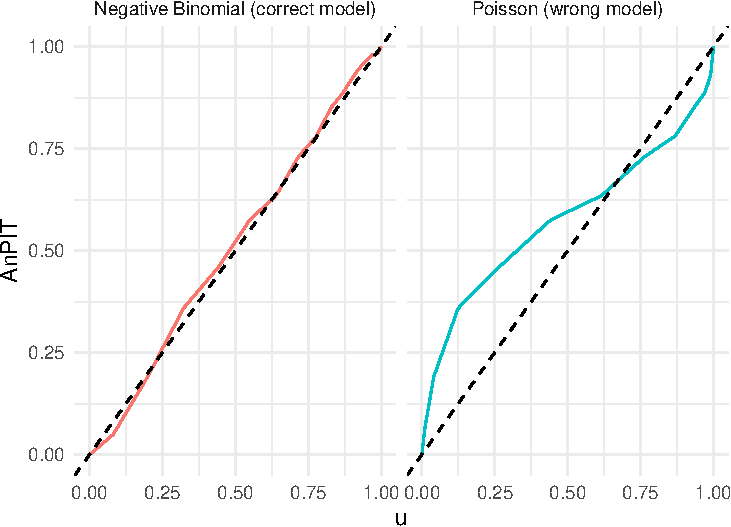
\includegraphics[keepaspectratio]{04_geostatistical-prediction_files/figure-pdf/fig-anpit-1.pdf}}

}

\caption{\label{fig-anpit}Average nonrandomized Probability Integral
Transform (AnPIT) applied to simulated data from a Negative Binomial
distribution. The left plot shows the AnPIT when the model is correctly
specified. The right panel shows the AnPIT when a Poisson model is
instead used. For more details we refer to the main text.}

\end{figure}%

Figure~\ref{fig-anpit} shows clear evidence that the Poisson model is
not adequately accounting for the overdispersion of the simulated data
from the Negative Binomial distribution.

How can we adapt this approach to generalized linear geostatistical
models (GLGMs)? The concept is straightforward, though the
implementation is less so (but fortunately, we have already done this in
\texttt{RiskMap}). Essentially, in all relevant equations above, we need
to replace \(M\) with the predictive distribution of the fitted
geostatistical model.

To explain further, suppose we have fitted our model using data
\(Y^{(1)} = \left( y^{(1)}_{1}, \ldots, y^{(1)}_{n} \right)\) (the
training data-set), and we want to use another set of data
\(Y^{(2)} = \left( y^{(2)}_{1}, \ldots, y^{(2)}_{m} \right)\) (the test
data-set) to assess calibration; the selection of \(Y^{(1)}\) and
\(Y^{(2)}\) can be done using the methods described in
Section~\ref{sec-split-data}. Our model \(M\) in the equations above
corresponds to the distribution of
\(\left[ Y^{(2)} \mid Y^{(1)} \right]\) -- the distribution of
\(Y^{(2)}\) conditioned to \(Y^{(1)}\) derived from our geostatistical
model. Since its derivation cannot be done analytically, we use Monte
Carlo methods to approximate \(\left[ Y^{(1)} \mid Y^{(2)} \right]\). We
discuss this in more detail in Section~\ref{sec-theory-prediction}.
However, the key point here is to understand why we perform this
assessment and how to interpret the results. We next show the
application of the AnPIT diagnostic to the example on riverblindess
mapping in Liberia.

\subsubsection{Example: assessing the calibration of two geostatistical
models for riverblindness mapping}\label{sec-liberia-anpit}

In our example on riverblindness mapping, we now consider two models. A
mode, which we call \(M_{0}\), which is an intercept only geostatistical
model, with linear predictor \[
M_{0} \: : \: \log\left\{\frac{p(x_i)}{1-p(x_i)}\right\} = \beta_0 + S(x_i) ,
\] and a geostatistical model, which we denote as \(M_{1}\), which uses
a linear spline with a not in 150 meters, and has linear predictor \[
M_{1} \: : \: \log\left\{\frac{p(x_i)}{1-p(x_i)}\right\} = \beta_0 + \beta_{1}e(x_i) + \beta_{2}\max\{e(x_i) - 150, 0\} + S(x_i).
\] The reason for using this type of linear spline in \(M_{1}\) is
explained in Section~\ref{sec-expl-assoc}.

Hence, we first fit the two models.

\begin{Shaded}
\begin{Highlighting}[]
\CommentTok{\# Fitting M0}
\FunctionTok{set.seed}\NormalTok{(}\DecValTok{123}\NormalTok{)}
\NormalTok{M0\_fit }\OtherTok{\textless{}{-}} 
\FunctionTok{glgpm}\NormalTok{(npos }\SpecialCharTok{\textasciitilde{}}  \FunctionTok{gp}\NormalTok{(long, lat, }\AttributeTok{nugget =} \ConstantTok{NULL}\NormalTok{),}
      \AttributeTok{den =}\NormalTok{ ntest, }\AttributeTok{data =}\NormalTok{ liberia,}
      \AttributeTok{crs =} \DecValTok{4326}\NormalTok{,}
      \AttributeTok{convert\_to\_crs =} \DecValTok{32629}\NormalTok{,}
      \AttributeTok{family =} \StringTok{"binomial"}\NormalTok{, }\AttributeTok{messages =} \ConstantTok{FALSE}\NormalTok{)}

\CommentTok{\# Fitting M1}
\NormalTok{M1\_fit }\OtherTok{\textless{}{-}} 
\FunctionTok{glgpm}\NormalTok{(npos }\SpecialCharTok{\textasciitilde{}}\NormalTok{  elevation }\SpecialCharTok{+} \FunctionTok{pmax}\NormalTok{(elevation }\SpecialCharTok{{-}} \DecValTok{150}\NormalTok{, }\DecValTok{0}\NormalTok{) }\SpecialCharTok{+}
      \FunctionTok{gp}\NormalTok{(long, lat, }\AttributeTok{nugget =} \ConstantTok{NULL}\NormalTok{),}
      \AttributeTok{den =}\NormalTok{ ntest, }\AttributeTok{data =}\NormalTok{ liberia,}
      \AttributeTok{crs =} \DecValTok{4326}\NormalTok{,}
      \AttributeTok{convert\_to\_crs =} \DecValTok{32629}\NormalTok{,}
      \AttributeTok{family =} \StringTok{"binomial"}\NormalTok{, }\AttributeTok{messages =} \ConstantTok{FALSE}\NormalTok{)}
\end{Highlighting}
\end{Shaded}

Since the main goal of this analysis is to draw predictive inference on
riverblindness prevalence within Liberia, it would be more appropriate
to use a regulirized subsampling scheme to split the data. To generate
the AnPIT diagnostic plot in R, we can use the \texttt{assess\_pp}
function in \texttt{RiskMap}

\begin{Shaded}
\begin{Highlighting}[]
\NormalTok{regularized }\OtherTok{\textless{}{-}} 
\FunctionTok{assess\_pp}\NormalTok{(}\FunctionTok{list}\NormalTok{(}\AttributeTok{M0 =}\NormalTok{ M0\_fit, }\AttributeTok{M1 =}\NormalTok{ M1\_fit),}
          \AttributeTok{which\_metric =} \StringTok{"AnPIT"}\NormalTok{, }
          \AttributeTok{method =} \StringTok{"regularized"}\NormalTok{, }\AttributeTok{min\_dist =} \DecValTok{20}\NormalTok{,}
          \AttributeTok{n\_size =} \DecValTok{9}\NormalTok{, }\AttributeTok{iter =} \DecValTok{10}\NormalTok{)}
\end{Highlighting}
\end{Shaded}

\begin{Shaded}
\begin{Highlighting}[]
\NormalTok{p1 }\OtherTok{\textless{}{-}} \FunctionTok{plot\_AnPIT}\NormalTok{(regularized, }\AttributeTok{combine\_panels =} \ConstantTok{TRUE}\NormalTok{) }\SpecialCharTok{+}
      \FunctionTok{theme}\NormalTok{(}\AttributeTok{plot.margin =} \FunctionTok{unit}\NormalTok{(}\FunctionTok{c}\NormalTok{(}\FloatTok{0.5}\NormalTok{, }\FloatTok{0.5}\NormalTok{, }\FloatTok{0.5}\NormalTok{, }\FloatTok{0.5}\NormalTok{), }\StringTok{"lines"}\NormalTok{)) }

\NormalTok{p2 }\OtherTok{\textless{}{-}} \FunctionTok{plot\_AnPIT}\NormalTok{(regularized, }\AttributeTok{mode =} \StringTok{"all"}\NormalTok{) }\SpecialCharTok{+}
      \FunctionTok{theme}\NormalTok{(}\AttributeTok{plot.margin =} \FunctionTok{unit}\NormalTok{(}\FunctionTok{c}\NormalTok{(}\FloatTok{0.5}\NormalTok{, }\FloatTok{0.5}\NormalTok{, }\FloatTok{0.5}\NormalTok{, }\FloatTok{0.5}\NormalTok{), }\StringTok{"lines"}\NormalTok{)) }

\FunctionTok{grid.arrange}\NormalTok{(p1, p2, }\AttributeTok{nrow =} \DecValTok{2}\NormalTok{, }\AttributeTok{heights =} \FunctionTok{c}\NormalTok{(}\DecValTok{1}\NormalTok{, }\DecValTok{1}\NormalTok{))}
\end{Highlighting}
\end{Shaded}

\begin{figure}[H]

\centering{

\pandocbounded{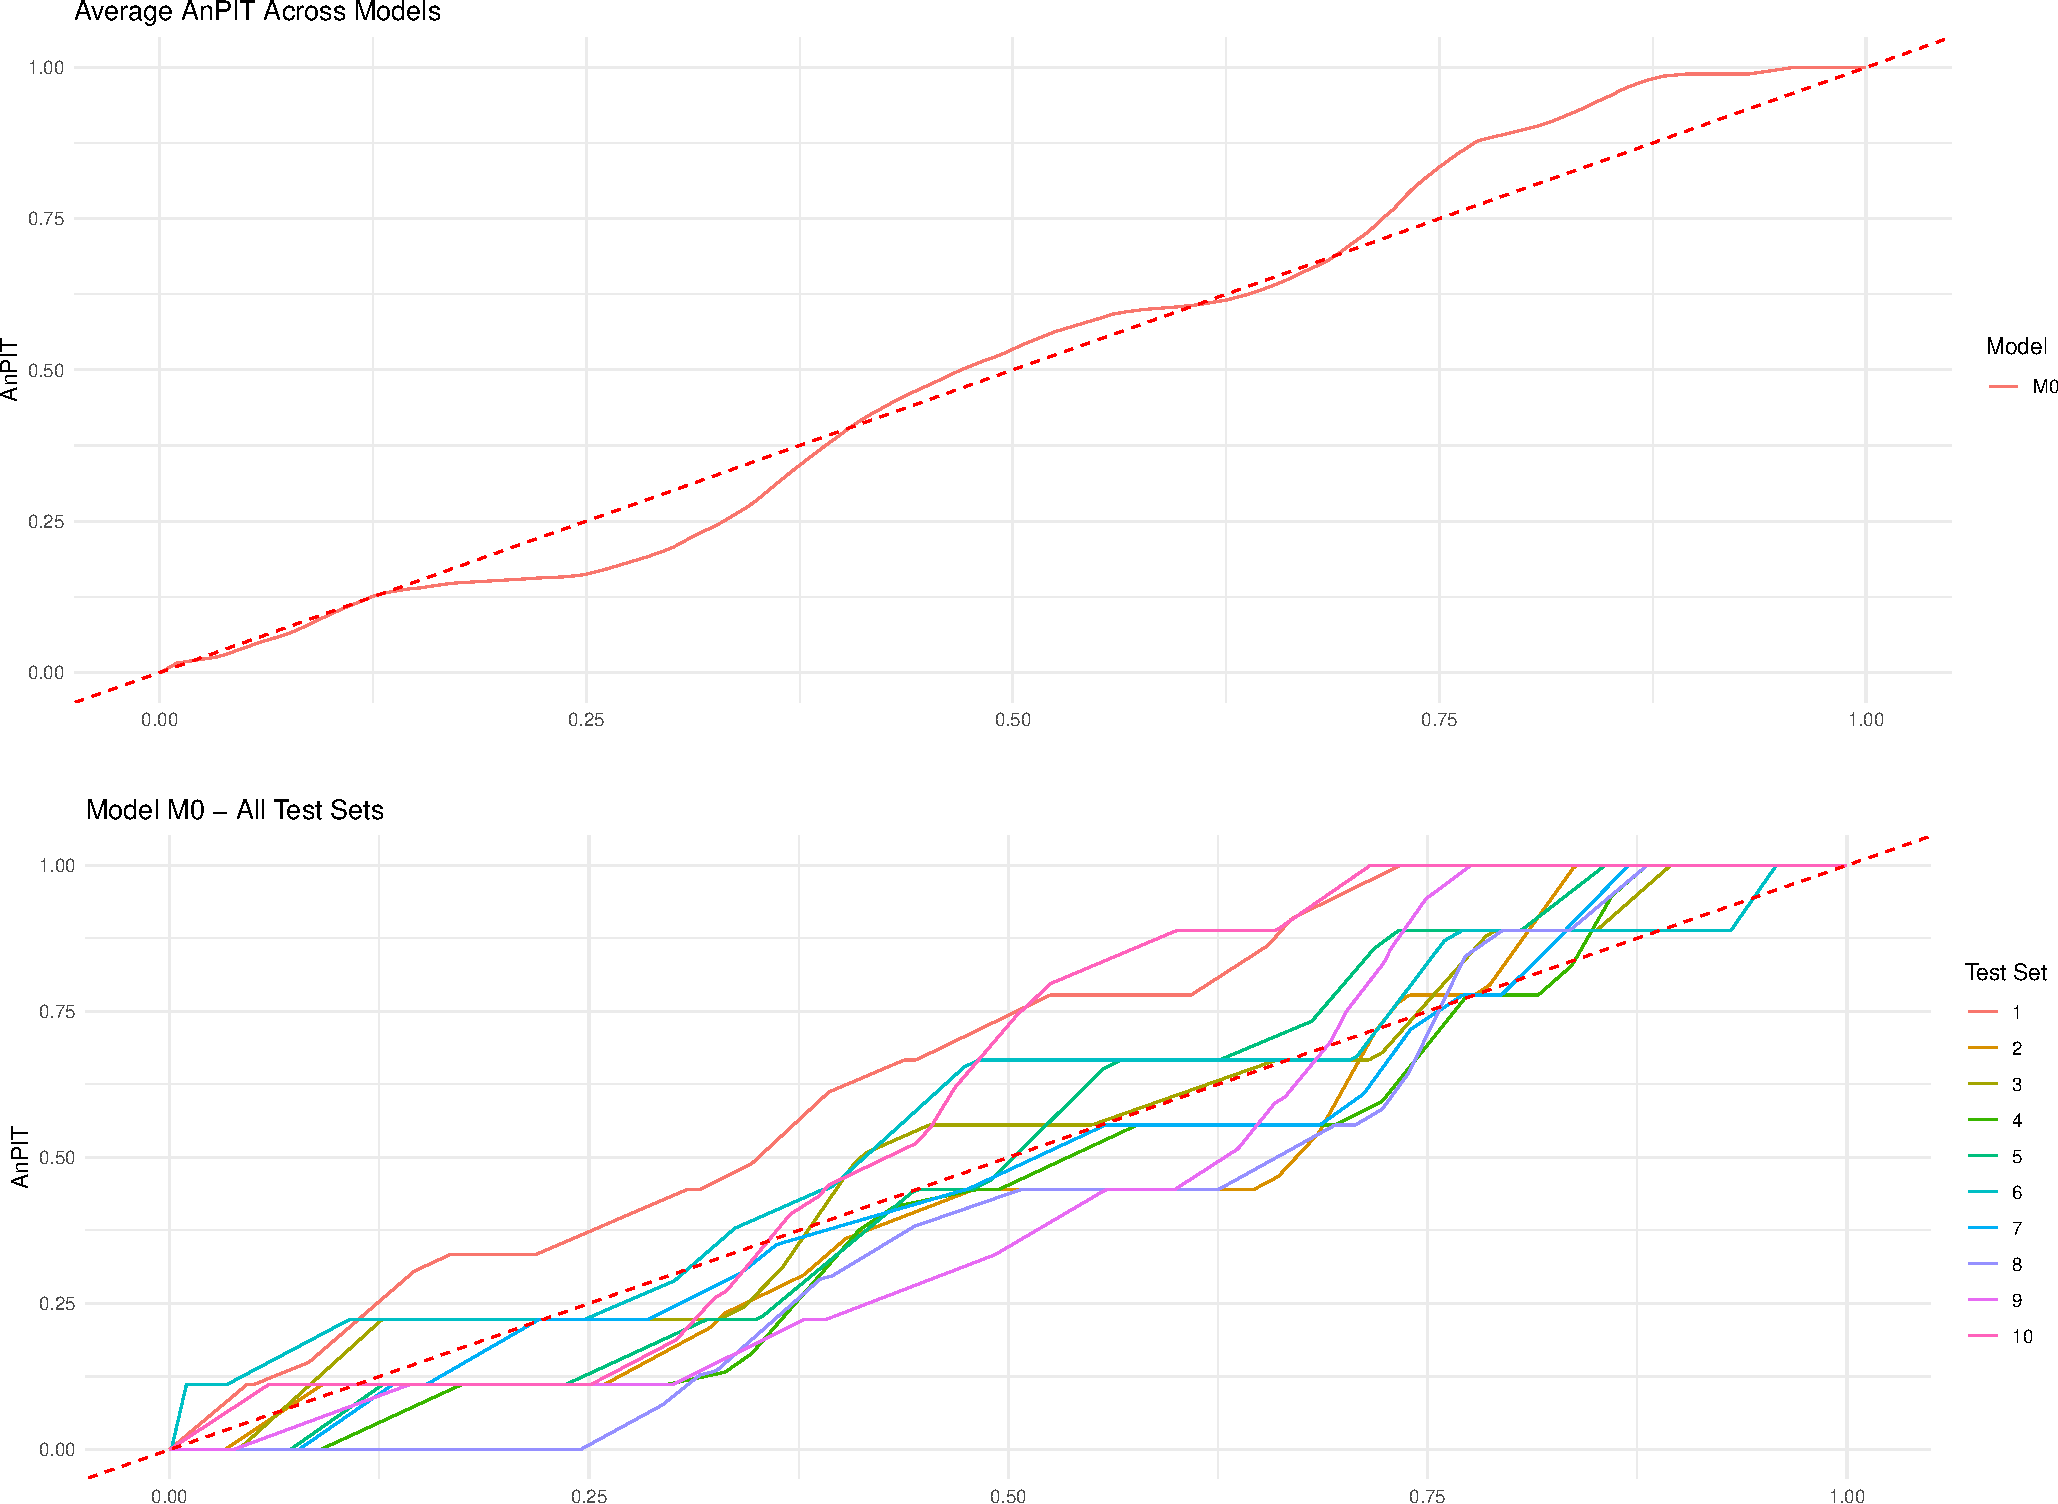
\includegraphics[keepaspectratio]{04_geostatistical-prediction_files/figure-pdf/fig-anpit-reg-1.pdf}}

}

\caption{\label{fig-anpit-reg}The average nonrandomized probability
integral transform (AnPIT) averaged across 10 test sets of size 9 (upper
panel) and for each of the 10 tests sets (lower panel). The test sets
are generated using a spatially regularized sampling scheme.}

\end{figure}%

In the above function, we have used a spatially regularized sampling
scheme (\texttt{method\ =\ "clusterized"}), where the locations are at
least 20 kilometers (\texttt{min\_dist\ =\ 20}) apart from each other to
create 10 test sets (\texttt{iter\ =\ 10}) each of size 9
(\texttt{n\_size\ =\ 9}) which corresponds to 10\% of the original
data-set. The results reported in Figure~\ref{fig-anpit-reg}, show both
the AnPIT for each of the 10 test sets and the averaged AnPIT across the
10 test sets, for both \(M_0\) and \(M_1\). The AnPIT plots show curves
that are not too far from the identity line, which leads us to conclude
that both \(M_0\) and \(M_1\) can be considered to be approximately well
calibrated models.

Let us how if these results would change if we were to split the data
using a clustering algorithm approach. We then use the
\texttt{assess\_pp}, to create 10 folds and set
\texttt{method\ =\ "cluster"}.

\begin{Shaded}
\begin{Highlighting}[]
\NormalTok{cluster }\OtherTok{\textless{}{-}} 
\FunctionTok{assess\_pp}\NormalTok{(}\FunctionTok{list}\NormalTok{(}\AttributeTok{M0 =}\NormalTok{ M0\_fit, }\AttributeTok{M1 =}\NormalTok{ M1\_fit),}
          \AttributeTok{which\_metric =} \StringTok{"AnPIT"}\NormalTok{, }
          \AttributeTok{method =} \StringTok{"cluster"}\NormalTok{, }\AttributeTok{fold =} \DecValTok{10}\NormalTok{)}
\end{Highlighting}
\end{Shaded}

\begin{Shaded}
\begin{Highlighting}[]
\NormalTok{p1 }\OtherTok{\textless{}{-}} \FunctionTok{plot\_AnPIT}\NormalTok{(cluster, }\AttributeTok{combine\_panels =} \ConstantTok{TRUE}\NormalTok{) }\SpecialCharTok{+}
      \FunctionTok{theme}\NormalTok{(}\AttributeTok{plot.margin =} \FunctionTok{unit}\NormalTok{(}\FunctionTok{c}\NormalTok{(}\FloatTok{0.5}\NormalTok{, }\FloatTok{0.5}\NormalTok{, }\FloatTok{0.5}\NormalTok{, }\FloatTok{0.5}\NormalTok{), }\StringTok{"lines"}\NormalTok{)) }\CommentTok{\# Tighter margins}

\NormalTok{p2 }\OtherTok{\textless{}{-}} \FunctionTok{plot\_AnPIT}\NormalTok{(cluster, }\AttributeTok{mode =} \StringTok{"all"}\NormalTok{) }\SpecialCharTok{+}
      \FunctionTok{theme}\NormalTok{(}\AttributeTok{plot.margin =} \FunctionTok{unit}\NormalTok{(}\FunctionTok{c}\NormalTok{(}\FloatTok{0.5}\NormalTok{, }\FloatTok{0.5}\NormalTok{, }\FloatTok{0.5}\NormalTok{, }\FloatTok{0.5}\NormalTok{), }\StringTok{"lines"}\NormalTok{)) }\CommentTok{\# Tighter margins}

\FunctionTok{grid.arrange}\NormalTok{(p1, p2, }\AttributeTok{nrow =} \DecValTok{2}\NormalTok{, }\AttributeTok{heights =} \FunctionTok{c}\NormalTok{(}\DecValTok{1}\NormalTok{, }\DecValTok{1}\NormalTok{)) }\CommentTok{\# Equal heights}
\end{Highlighting}
\end{Shaded}

\begin{figure}[H]

\centering{

\pandocbounded{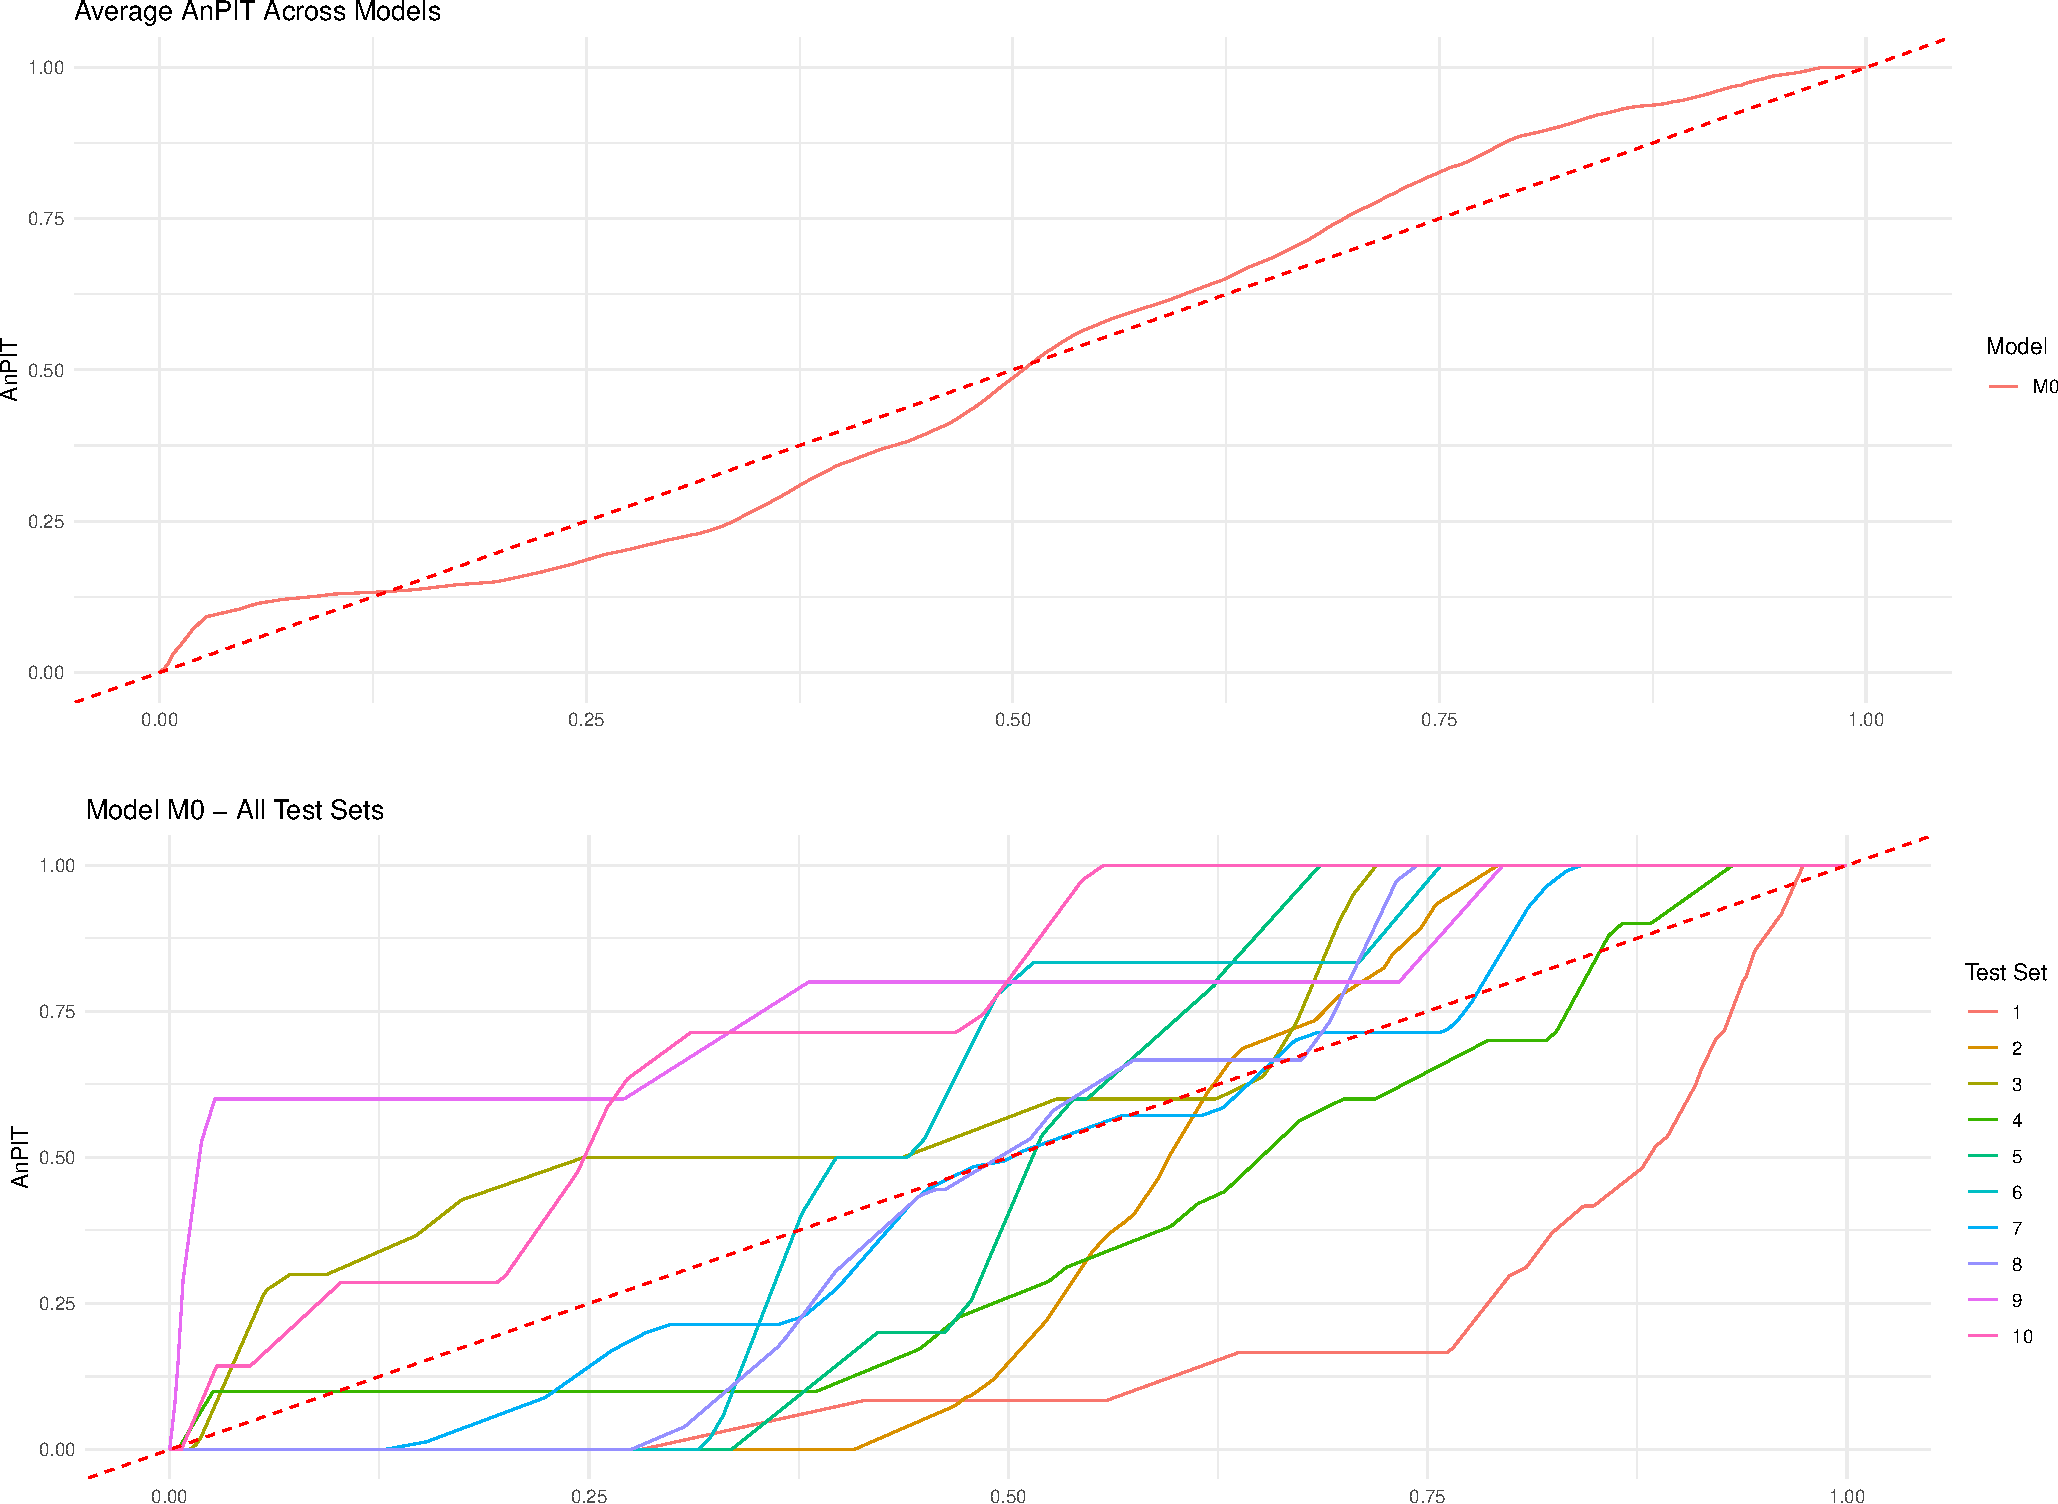
\includegraphics[keepaspectratio]{04_geostatistical-prediction_files/figure-pdf/fig-anpit-clus-1.pdf}}

}

\caption{\label{fig-anpit-clus}The average nonrandomized probability
integral transform (AnPIT) averaged across 10 test sets of size 9 (upper
panel) and for each of the 10 test sets (lower panel). The test sets are
generated using a clustering algorithm based on the locations of the
data.}

\end{figure}%

The AnPIT from Figure~\ref{fig-anpit-clus} show very similar results to
those of Figure~\ref{fig-anpit-reg}, hence similar conclusions are
drawn.

\subsection{Assessing calibration and sharpness using continuous ranked
probability
scores}\label{assessing-calibration-and-sharpness-using-continuous-ranked-probability-scores}

We now consider another important aspect that helps to describe the
predictive performance of a geostatistical model, namely sharpness. As
the name suggests, sharpness refers to the spread of the predictive
distribution. A sharp predictive distribution has a narrow spread,
indicating that the model is highly confident in its predictions.
Importantly, sharpness does not depend on how close predictions are to
the true values (i.e., it is independent of accuracy). A model with high
sharpness will produce predictions with low variance, but this sharpness
is only meaningful if the model is well-calibrated, ensuring that the
high confidence aligns with observed values. For example, a
geostatistical model for disease prevalence mapping that predicts a very
tight range of possible prevalence values for a location is producing
sharp predictions. However, if the actual prevalence often falls outside
this range, then the predictions may be sharp but poorly calibrated,
thus limiting the value of quantifying sharpness alone.

To assess predictive performance while considering both \emph{sharpness}
and \emph{calibration}, we introduce the \emph{continuous ranked
probability score (CRPS)} (Gneiting, Balabdaoui, and Raftery 2007) and
its scaled variant, the \emph{scaled CRPS (SCRPS)} (Bolin and Wallin
2023). The CRPS evaluates the agreement between the predicted cumulative
distribution function of the model \(M\), denoted as in the previous
section by \(F_M\), and the observed value \(y_i\). It is formally
defined as

\[
\text{CRPS}(F_M, y_i) = \int_{-\infty}^\infty \left[ F_M(y) - \mathbf{1}(y \geq y_i) \right]^2 dy,
\]

penalizing deviations of the predictive distribution from the observed
value. The CRPS balances sharpness and calibration, with smaller values
indicating better predictive performance.

The \emph{scaled CRPS (SCRPS)}, proposed by Bolin and Wallin (2023),
refines the CRPS by addressing its dependence on the scale of the
outcome variable, which can vary across observations. The SCRPS is
defined as

\begin{equation}\phantomsection\label{eq-scrps}{
\text{SCRPS}(F_M, y_i) = -\frac{1}{2} \left[ 1 + \frac{\text{CRPS}(F_M, y_i)}{\text{CRPS}(F_M, F_M)} + \log\left\{2 \, \text{CRPS}(F_M, F_M)\right\} \right],
}\end{equation}

where \(\text{CRPS}(F_M, F_M)\) denotes the expected CRPS when the
observation is drawn from the predictive distribution itself, i.e.,
\(Y \sim F_M\).

In settings where the predictive distribution is discrete, such as the
Binomial and Poisson geostatistical models, a discrete analogue to CRPS
is used. Let \(F_M(k)\) be the cumulative distribution function over
discrete support \(\{0, 1, 2, \dots\}\). The discrete CRPS is given by

\[
\text{CRPS}(F_M, y_i) = \sum_{k \in \mathcal{S}}^{\infty} \left[ F_M(k) - \mathbf{1}(k \geq y_i) \right]^2,
\]

where \(\mathcal{S}\) represents the support of the outcome \(Y_{i}\),
corresponding to \(\{0,1,\ldots,m_i\}\) for the Binomial distribution,
and the set of non-negative integers as in a Poisson distribution. This
version remains proper and interpretable as a measure of calibration and
sharpness for integer-valued outcomes. Analogously, a scaled version of
the discrete CRPS can be constructed using the same transformation as in
the continuous case, by replcing the continuous CRPS with its discrete
counterpart in Equation~\ref{eq-scrps}.

providing a scale-invariant and proper scoring rule for discrete
predictive models. These discrete versions are particularly useful in
count data models or models for ordinal responses.

The expressions for the CRPS and SCRPS may initially appear complex, but
their appropriate application and interpretation lie in understanding
their differences and the contexts in which each is more suitable. These
differences become more intuitive when considering the more familiar
concept of the standard error. The standard error of a predictive
distribution represents its uncertainty, but it is not inherently
standardized. In many cases, there exists a mean-variance relationship,
where the variance increases with the mean. For instance, in
Poisson-distributed data, higher mean values correspond to larger
variances. This lack of standardization means that directly comparing
predictive uncertainties across different scales can be misleading.
Similarly, the CRPS is sensitive to the scale of the predictive
distribution, as it penalizes errors in absolute terms, often giving
disproportionate weight to observations with larger predictive
uncertainty.

The SCRPS addresses this issue by standardizing predictive errors
relative to the expected spread of the predictive distribution, ensuring
\emph{local scale invariance}. This means that the penalty for an
incorrect prediction is adjusted proportionally to the scale of the
predictive distribution. As a result, the SCRPS enables meaningful
comparisons across observations with varying levels of uncertainty. To
draw an analogy, the SCRPS standardizes the CRPS in much the same way
that the coefficient of variation (CV) standardizes the standard error.
By dividing the standard error by the mean of the predictive
distribution, the CV expresses variability relative to the mean. This
property is particularly valuable in geostatistical applications, where
uncertainty often varies spatially due to factors such as
non-stationarity of the predictive distribution or irregularly spaced
observations.

However, while the SCRPS is more robust in settings where variability
differs significantly across observations, there are contexts where the
CRPS may be preferred. Specifically, in cases where greater emphasis
should be placed on accurately predicting observations with larger
uncertainty, the CRPS is more appropriate because it assigns greater
weight to predictions with higher variance. For example, as highlighted
in Bolin and Wallin (2023), when forecasting rare but impactful events
(e.g., extreme weather conditions), the larger uncertainties associated
with these events may naturally demand greater attention. In such
scenarios, the CRPS's sensitivity to scale can be an advantage, as it
prioritizes minimizing errors for these high-variance predictions.

When evaluating the predictive performance of a model \(M\), we proceed
as follows. Let \(\left(x_{1}^{(i)}, \ldots, x_{m_i}^{(i)}\right)\)
represent the set of locations in the \(i\)-th test set, for
\(i=1, \ldots, T\). For each location, we compute the score---either
CRPS or SCRPS---and denote it as \(r_{M}\left(x_{j}^{(i)}\right)\).

To assess the overall performance of model \(M\), we calculate a
weighted average of the scores across all test sets, where the weights
are proportional to the sample size of each test set. The final score
assigned to model \(M\) is given by:
\begin{equation}\phantomsection\label{eq-average-score}{
\frac{1}{\sum_{i=1}^T m_i} \sum_{i=1}^{T} \sum_{j=1}^{m_i} r_{M}\left(x_{j}^{(i)}\right). }\end{equation}

Models assumed to be well-calibrated and achieving a lower score based
on the above expression are considered to provide sharper predictions
and, consequently, better predictive performance.

\subsubsection{\texorpdfstring{Example: mapping riverblindness in
Liberia (continuing from
Section~\ref{sec-liberia-anpit})}{Example: mapping riverblindness in Liberia (continuing from Section~)}}\label{example-mapping-riverblindness-in-liberia-continuing-from-sec-liberia-anpit}

In Section~\ref{sec-liberia-anpit}, we have assessed the calibration of
models \(M_0\) and \(M_0\) and found these to be reasonably well
calibrated models. We now compare the predictive performance of the two,
using both the CRPS and SCRPS metrics introduced previously.

The \texttt{assess\_pp} function also allows the user to compute the
CRPS and SCRPS through the argument \texttt{which\_metric} as shown
below.

\begin{Shaded}
\begin{Highlighting}[]
\NormalTok{regularized\_scores }\OtherTok{\textless{}{-}} 
\FunctionTok{assess\_pp}\NormalTok{(}\FunctionTok{list}\NormalTok{(}\AttributeTok{M0 =}\NormalTok{ M0\_fit, }\AttributeTok{M1 =}\NormalTok{ M1\_fit),}
          \AttributeTok{which\_metric =} \FunctionTok{c}\NormalTok{(}\StringTok{"CRSP"}\NormalTok{, }\StringTok{"SCRPS"}\NormalTok{), }
          \AttributeTok{method =} \StringTok{"regularized"}\NormalTok{, }\AttributeTok{min\_dist =} \DecValTok{20}\NormalTok{,}
          \AttributeTok{n\_size =} \DecValTok{9}\NormalTok{, }\AttributeTok{iter =} \DecValTok{10}\NormalTok{)}

\NormalTok{cluster\_scores }\OtherTok{\textless{}{-}} 
\FunctionTok{assess\_pp}\NormalTok{(}\FunctionTok{list}\NormalTok{(}\AttributeTok{M0 =}\NormalTok{ M0\_fit, }\AttributeTok{M1 =}\NormalTok{ M1\_fit),}
          \AttributeTok{which\_metric =} \FunctionTok{c}\NormalTok{(}\StringTok{"CRSP"}\NormalTok{, }\StringTok{"SCRPS"}\NormalTok{), }
          \AttributeTok{method =} \StringTok{"cluster"}\NormalTok{, }\AttributeTok{fold =} \DecValTok{10}\NormalTok{)}
\end{Highlighting}
\end{Shaded}

Note that that \texttt{assess\_pp} can be run once in order to obtain
both the AnPIT diagnostic, introduced in Section~\ref{sec-anpit}; by
default \texttt{which\_metric\ =\ c("AnPIT",\ "CRSP",\ "SCRPS")} which
computes all three diagnostic using the same test sets. The reason we
have separated the AnPIT and the scores computations is only for
pedagogical purposes.

By doing a \texttt{summary} of the output in
\texttt{regularized\_scores} and \texttt{cluster\_scores}, we obtain the
average score across all test sets as defined in
Equation~\ref{eq-average-score}.

\begin{Shaded}
\begin{Highlighting}[]
\FunctionTok{summary}\NormalTok{(regularized\_scores, }\AttributeTok{view\_all =} \ConstantTok{FALSE}\NormalTok{)}
\DocumentationTok{\#\# Summary of Cross{-}Validation Scores}
\DocumentationTok{\#\# {-}{-}{-}{-}{-}{-}{-}{-}{-}{-}{-}{-}{-}{-}{-}{-}{-}{-}{-}{-}{-}{-}{-}{-}{-}{-}{-}{-}{-}{-}{-}{-}{-}{-}}
\DocumentationTok{\#\# Model: M0}
\DocumentationTok{\#\#   Overall average across test sets:}
\DocumentationTok{\#\#     CRPS: {-}0.0384}
\DocumentationTok{\#\#     SCRPS: 0.2488}
\DocumentationTok{\#\# }
\DocumentationTok{\#\# Model: M1}
\DocumentationTok{\#\#   Overall average across test sets:}
\DocumentationTok{\#\#     CRPS: {-}0.0415}
\DocumentationTok{\#\#     SCRPS: 0.2091}

\FunctionTok{summary}\NormalTok{(cluster\_scores, }\AttributeTok{view\_all =} \ConstantTok{FALSE}\NormalTok{)}
\DocumentationTok{\#\# Summary of Cross{-}Validation Scores}
\DocumentationTok{\#\# {-}{-}{-}{-}{-}{-}{-}{-}{-}{-}{-}{-}{-}{-}{-}{-}{-}{-}{-}{-}{-}{-}{-}{-}{-}{-}{-}{-}{-}{-}{-}{-}{-}{-}}
\DocumentationTok{\#\# Model: M0}
\DocumentationTok{\#\#   Overall average across test sets:}
\DocumentationTok{\#\#     CRPS: {-}0.0464}
\DocumentationTok{\#\#     SCRPS: 0.1635}
\DocumentationTok{\#\# }
\DocumentationTok{\#\# Model: M1}
\DocumentationTok{\#\#   Overall average across test sets:}
\DocumentationTok{\#\#     CRPS: {-}0.0446}
\DocumentationTok{\#\#     SCRPS: 0.1683}
\end{Highlighting}
\end{Shaded}

In the code above, we have set \texttt{view\_all\ =\ FALSE} to display
only the overall average. If \texttt{view\_all\ =\ TRUE}, the scores are
instead reported for each test set, in addition to the overall average.
The results from the \texttt{summary} suggest that the two models have a
similar predictive performance in terms of both CRPS and SCRPS,
regardless of the sampling scheme used to create the test sets. To
examine this further we can plot a point map of the CRPS and SCRPS using
the locations of the test sets.

\begin{Shaded}
\begin{Highlighting}[]
\CommentTok{\# Define ranges for the color scales}

\NormalTok{crps\_range }\OtherTok{\textless{}{-}} \FunctionTok{range}\NormalTok{(}\FunctionTok{c}\NormalTok{(}\FunctionTok{unlist}\NormalTok{(cluster\_scores}\SpecialCharTok{$}\NormalTok{model}\SpecialCharTok{$}\NormalTok{M0}\SpecialCharTok{$}\NormalTok{score}\SpecialCharTok{$}\NormalTok{CRPS),}
                      \FunctionTok{unlist}\NormalTok{(cluster\_scores}\SpecialCharTok{$}\NormalTok{model}\SpecialCharTok{$}\NormalTok{M1}\SpecialCharTok{$}\NormalTok{score}\SpecialCharTok{$}\NormalTok{CRPS)))  }
\NormalTok{scrps\_range }\OtherTok{\textless{}{-}} \FunctionTok{range}\NormalTok{(}\FunctionTok{c}\NormalTok{(}\FunctionTok{unlist}\NormalTok{(cluster\_scores}\SpecialCharTok{$}\NormalTok{model}\SpecialCharTok{$}\NormalTok{M0}\SpecialCharTok{$}\NormalTok{score}\SpecialCharTok{$}\NormalTok{SCRPS),}
                      \FunctionTok{unlist}\NormalTok{(cluster\_scores}\SpecialCharTok{$}\NormalTok{model}\SpecialCharTok{$}\NormalTok{M1}\SpecialCharTok{$}\NormalTok{score}\SpecialCharTok{$}\NormalTok{SCRPS))) }

\CommentTok{\# Generate the plots with consistent color scales}
\NormalTok{p1 }\OtherTok{\textless{}{-}} \FunctionTok{plot\_score}\NormalTok{(cluster\_scores, }
                 \AttributeTok{which\_score =} \StringTok{"CRPS"}\NormalTok{, }\AttributeTok{which\_model =} \StringTok{"M0"}\NormalTok{) }\SpecialCharTok{+}  
      \FunctionTok{scale\_color\_viridis\_c}\NormalTok{(}\AttributeTok{option =} \StringTok{"C"}\NormalTok{, }
      \AttributeTok{limits =}\NormalTok{ crps\_range, }\AttributeTok{direction =} \DecValTok{1}\NormalTok{) }
\NormalTok{p2 }\OtherTok{\textless{}{-}} \FunctionTok{plot\_score}\NormalTok{(cluster\_scores, }
                 \AttributeTok{which\_score =} \StringTok{"CRPS"}\NormalTok{, }\AttributeTok{which\_model =} \StringTok{"M1"}\NormalTok{) }\SpecialCharTok{+}       
      \FunctionTok{scale\_color\_viridis\_c}\NormalTok{(}\AttributeTok{option =} \StringTok{"C"}\NormalTok{, }
      \AttributeTok{limits =}\NormalTok{ crps\_range, }\AttributeTok{direction =} \DecValTok{1}\NormalTok{) }
\NormalTok{p3 }\OtherTok{\textless{}{-}} \FunctionTok{plot\_score}\NormalTok{(cluster\_scores, }
                 \AttributeTok{which\_score =} \StringTok{"SCRPS"}\NormalTok{, }\AttributeTok{which\_model =} \StringTok{"M0"}\NormalTok{) }\SpecialCharTok{+}  
      \FunctionTok{scale\_color\_viridis\_c}\NormalTok{(}\AttributeTok{option =} \StringTok{"C"}\NormalTok{, }
      \AttributeTok{limits =}\NormalTok{ scrps\_range, }\AttributeTok{direction =} \DecValTok{1}\NormalTok{) }
\NormalTok{p4 }\OtherTok{\textless{}{-}} \FunctionTok{plot\_score}\NormalTok{(cluster\_scores, }
                 \AttributeTok{which\_score =} \StringTok{"SCRPS"}\NormalTok{, }\AttributeTok{which\_model =} \StringTok{"M1"}\NormalTok{) }\SpecialCharTok{+}
      \FunctionTok{scale\_color\_viridis\_c}\NormalTok{(}\AttributeTok{option =} \StringTok{"C"}\NormalTok{, }
      \AttributeTok{limits =}\NormalTok{ scrps\_range, }\AttributeTok{direction =} \DecValTok{1}\NormalTok{) }
\FunctionTok{grid.arrange}\NormalTok{(p1, p2, p3, p4, }\AttributeTok{nrow =} \DecValTok{2}\NormalTok{, }\AttributeTok{ncol =} \DecValTok{2}\NormalTok{)}
\end{Highlighting}
\end{Shaded}

\begin{figure}[H]

\centering{

\pandocbounded{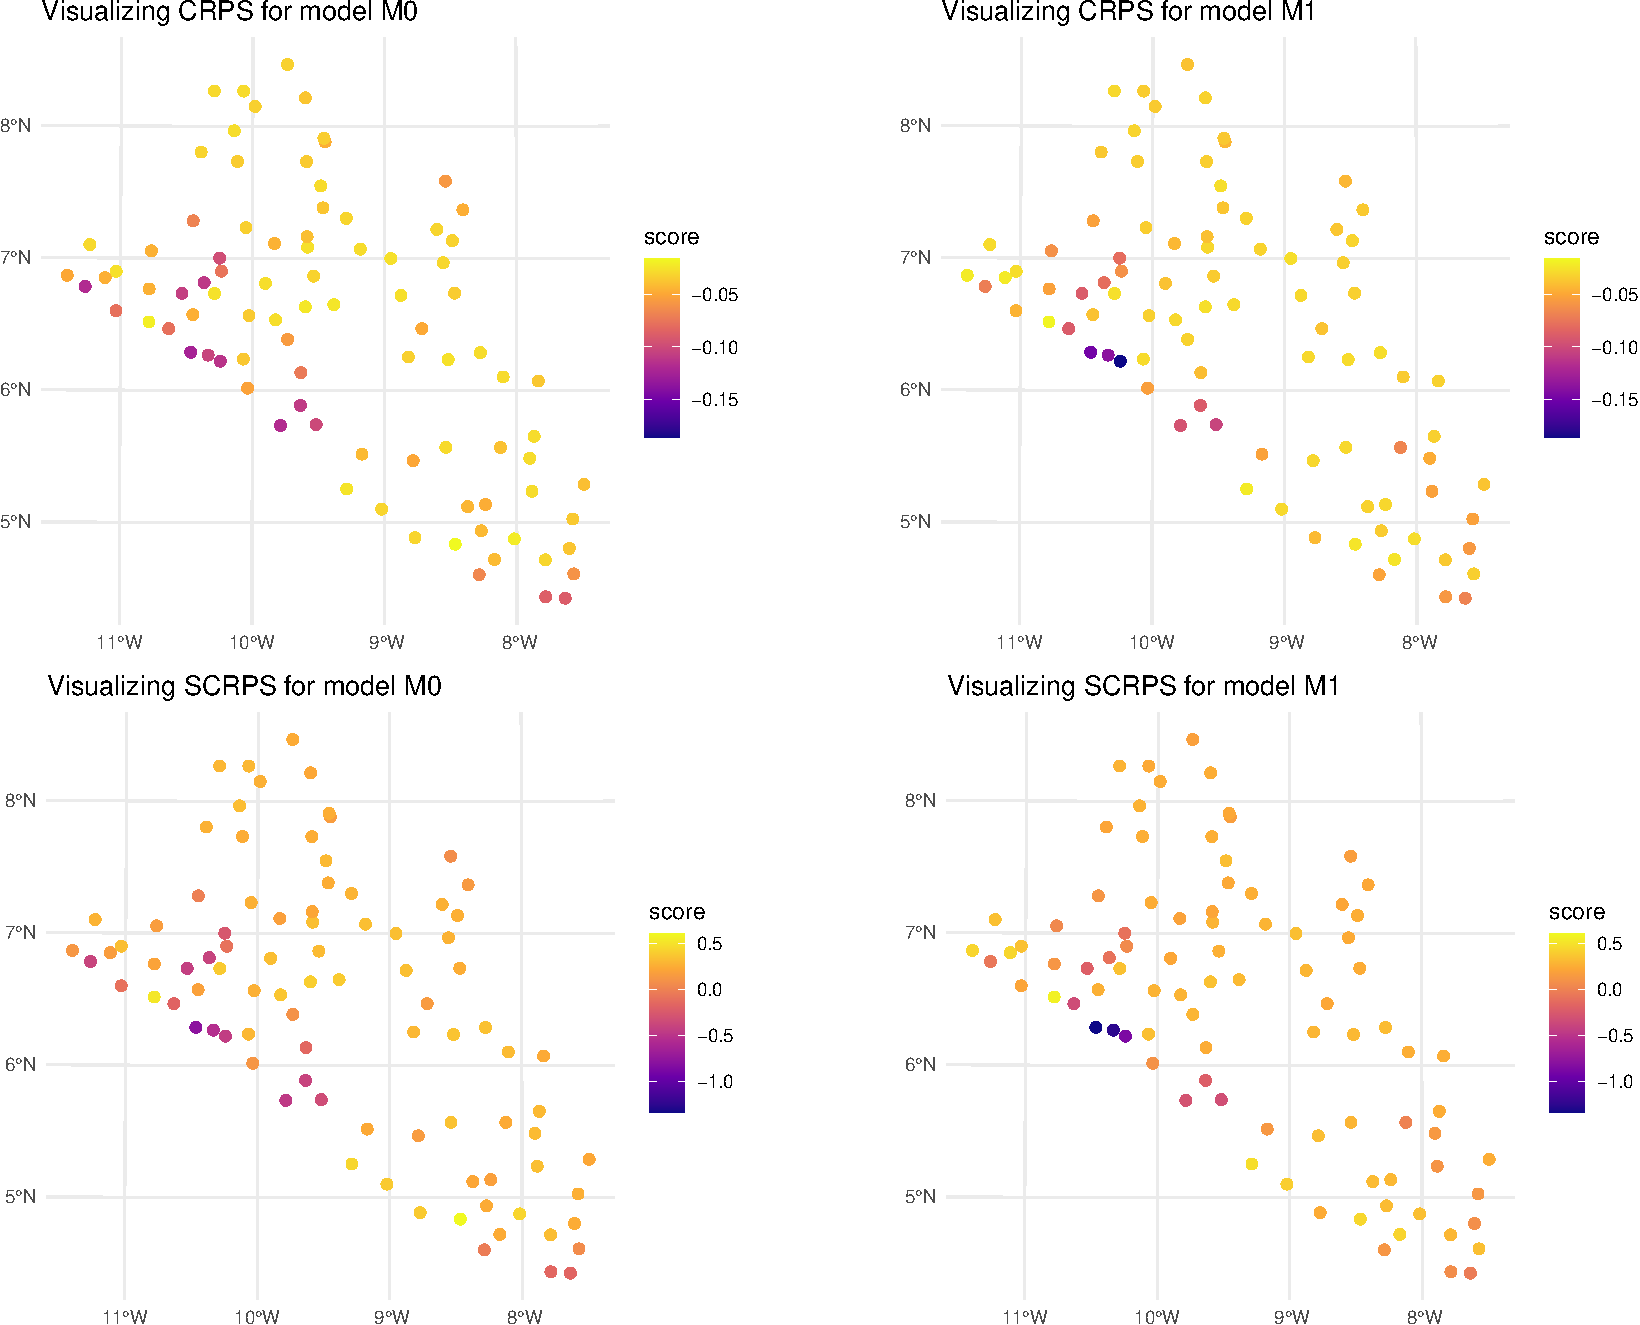
\includegraphics[keepaspectratio]{04_geostatistical-prediction_files/figure-pdf/fig-scores-map-1.pdf}}

}

\caption{\label{fig-scores-map}Point maps of the scores for model
\(M_{0}\) and \(M_{1}\) across the test sets generated using a clusering
approach for splitting the data. The upper panels are the map for the
continuous ranked probability score (CRPS) and the lower panels for the
scale CRPS (SCRPS).}

\end{figure}%

In the code above, we evaluated the cross-validation results generated
using a clustering algorithm to split the original data-set. The map
reveals that the scores across most locations are generally similar,
with only three locations near the coast of Liberia showing slightly
lower CRPS and SCRPS values for \(M_1\). This suggests a consistent
predictive performance across the dataset, with some localized
variations.

\section{Simulation-based assessment of predictive
performance}\label{simulation-based-assessment-of-predictive-performance}

In Section~\ref{sec-compare-pp}, we illustrated how to evaluate
predictive performance in relative terms, specifically by comparing
candidate models under consideration. In this section, we demonstrate
how simulation studies can be used to assess the predictive performance
of a geostatistical model in predicting a spatially continuous target
within a region of interest. Since a spatially continuous target cannot
be directly observed, simulations provide a way to generate such targets
under specified assumptions. This approach allows us to evaluate how
effectively the model can recover the underlying spatial surface using
suitable predictive performance metrics.

\subsection{Step 1: Define the aim of the simulation
study}\label{sec-sim-step1}

As previously stated, one of the main reasons for carrying out a
simulation study is the ability to generate spatial surfaces, which are
typically unobservable in the real world. The purpose of the simulation
is generally to evaluate how well a given geostatistical model can
recover that surface and/or draw inferences on some of its properties.

To fully understand the how to carry out a simulation study, it is
essential to define its two main components: the \emph{true model} and
the \emph{candidate models} (which can indeed include multiple options).

The \textbf{true model} represents the underlying stochastic process
that generates the data. In a simulation study, the true model is
assumed to be known because it is explicitly specified by us. It serves
as the benchmark against which other models are assessed.

The \textbf{candidate models} are the geostatistical models that are
tested or evaluated during the simulation study. These models are
proposed alternatives to approximate or recover the true spatial surface
or its properties. Candidate models may differ in terms of their
assumptions and model complexity.

It is important to highlight that the true model not only serves as a
benchmark but can also be included among the candidate models. However,
the true model does not always necessarily outperform other candidate
models. In some cases, certain candidate models may provide better
approximations of the spatial surface or its properties, particularly
when the true model's complexity is too high relative to the available
sample size. Here, \emph{model complexity} refers to the number of
parameters in a model. For instance, a true geostatistical model with
high complexity may include numerous covariates or a highly
parameterised covariance function. When the sample size is insufficient
to reliably estimate these parameters, simpler candidate models can
sometimes yield better performances.

Consider an extreme example where the true model is a spatial Gaussian
process \(S(x)\) with a scale parameter of \(\phi = 1\). If only a very
small fraction of sampled locations are at distances below 1, estimating
\(\phi\) accurately becomes highly challenging, especially with a small
sample size. In particular the sparsity of close pairs reduces the
information available to estimate the spatial dependence structure,
making the estimation of \(\phi\) imprecise or even unreliable. In this
case, a candidate model that does not attempt to explicitly estimate the
spatial dependence (e.g., a model that relies solely on spatial
covariates to interpolate the surface) might perform better in
recovering the spatial structure. This example suggests that a simpler
or alternative model can sometimes outperform the true model under
specific sampling and data constraints.

At this point, a natural question arises: how should we choose the true
model for a simulation study? The answer depends on the specific
objectives of the study and what we aim to demonstrate. We now provide
an example to demonstrate this point.

\subsubsection{Example}\label{example}

In our analysis of the river blindness dataset, we now aim to evaluate
the effectiveness of using elevation as a spatial predictor. To achieve
this, we conduct a simulation study to compare the performance of two
geostatistical models: one that incorporates elevation as a predictor
and another that excludes it. This example will be revisited throughout
the steps outlined in this section on simulation. We can chose the
following true model (henceforth \(M_T\)) for the simulation
\begin{equation}\phantomsection\label{eq-true-model-lib}{M_{T}: \:
\log\left\{\frac{p(x_i)}{1-p(x_i)}\right\} = \beta_{0} + \beta_{1}e(x_i) + \beta_{2}\max\{e(x_i)-150, 0\} + S(x_i).
}\end{equation} The true model, described by the equation above, assumes
a nonlinear relationship with elevation based on a linear spline with a
single knot at 150 meters. To simulate data from the true model, which
constitutes the next step in our simulation study, we must first define
the model parameter values. A reasonable approach is to use the maximum
likelihood estimates obtained by fitting the binomial geostatistical
model specified in Equation~\ref{eq-true-model-lib}. These estimates can
be derived as shown below.

\begin{Shaded}
\begin{Highlighting}[]
\FunctionTok{set.seed}\NormalTok{(}\DecValTok{123}\NormalTok{)}
\NormalTok{true\_model }\OtherTok{\textless{}{-}} \FunctionTok{glgpm}\NormalTok{(npos }\SpecialCharTok{\textasciitilde{}}\NormalTok{ elevation }\SpecialCharTok{+} \FunctionTok{pmax}\NormalTok{(elevation }\SpecialCharTok{{-}} \DecValTok{150}\NormalTok{, }\DecValTok{0}\NormalTok{) }\SpecialCharTok{+} 
                           \FunctionTok{gp}\NormalTok{(long, lat),}
                    \AttributeTok{den =}\NormalTok{ ntest,}
                    \AttributeTok{crs =} \DecValTok{4326}\NormalTok{, }
                    \AttributeTok{convert\_to\_crs =} \DecValTok{32629}\NormalTok{,}
                    \AttributeTok{family =} \StringTok{"binomial"}\NormalTok{,}
                    \AttributeTok{data =}\NormalTok{ liberia)}
\end{Highlighting}
\end{Shaded}

\begin{Shaded}
\begin{Highlighting}[]
\CommentTok{\# The parameters of the true model}
\FunctionTok{coef}\NormalTok{(true\_model)}
\end{Highlighting}
\end{Shaded}

\begin{verbatim}
$beta
             (Intercept)                elevation pmax(elevation - 150, 0) 
            -2.002985655              0.003160402             -0.001706721 

$sigma2
[1] 0.3181267

$phi
[1] 41.02334
\end{verbatim}

A natural candidate model to evaluate the usefulness of elevation as a
covariate is an intercept-only model (referred to here as \(M_C\)). This
model is defined as: \[M_{C}: \:
\log\left\{\frac{p(x_i)}{1-p(x_i)}\right\} = \beta_{0} + S(x_i).
\] where no covariates are included. This approach makes \(M_C\) a
suitable baseline model, commonly selected when the objective is to
assess the contribution of covariates to spatial prediction.

\subsection{Step 2: Simulate the spatial surface and the data from the
true
model}\label{step-2-simulate-the-spatial-surface-and-the-data-from-the-true-model}

In Section~\ref{sec-bootstrap}, we have shown how to simulate from a
geostatistical model, when the goal is simulate data at the observed
locations. When we want to simulate a spatial surface, a similar
approach can be used. First of all, we need to generate a regular grid,
say \(\tilde{X}\), covering the study region of interest, say \(A\).
Based on the notation used so far, we use \(X\) to denote the set of
observed locations which are used to simulate the outcome data \(Y\).
Finally, we use \(X_{+} = (X, \tilde{X})\) to denote the full set of
locations both on the grid and at the data points. We can then proceed
through the following steps to simultaneously simulate values of the
surface of interest over \(\tilde{X}\) and \(X\).

\begin{enumerate}
\def\labelenumi{\arabic{enumi}.}
\item
  Compute the covariance matrix \(\Sigma_{+}\) using the combined set of
  locations \(X_{+}\).
\item
  If covariates are used, compute the covariates effects
  \(d(x)^\top \beta\) for all the locations in \(X_{+}\).
\item
  Simulate \(B\)-times from a multivariate Gaussian distribution with
  mean vector 0 and covariance \(\Sigma_{+}\) as previously defined. We
  denote the output form this step as \(S_{(j)}(\tilde{x})\), for
  simulations generate on \(\tilde{X}\), and with \(S_{(j)}(x)\) for
  simulations on \(X\), respectively, for \(j=1,\ldots,B\).
\item
  Compute the linear predictor at each locations of \(X_{+}\), by adding
  the covariates effects in 3 to the simulated random effects in 4,
  hence
  \(g\{\mu_{(j)}(\tilde{x})\} = d(\tilde{x})^\top + S_{(j)}(\tilde{x})\)
  for \(\tilde{X}\), and \(g\{\mu_{(j)}(x)\} = d(x)^\top + S_{(j)}(x)\)
  for \(X\).
\item
  Only for locations of the data \(X\), perform the steps 5A to 7A as
  explained in Section~\ref{sec-bootstrap}, to simulate the data \(Y\).
\end{enumerate}

The function \texttt{surf\_sim} in \texttt{RiskMap} can be used to carry
out all these steps automatically as shown next.

\subsubsection{Example}\label{example-1}

Following the steps previously outlined, we first create a grid within
the boundaries of Liberia and extract the values of elevation on the
grid from a raster.

\begin{Shaded}
\begin{Highlighting}[]
\FunctionTok{library}\NormalTok{(rgeoboundaries)}
\NormalTok{shp }\OtherTok{\textless{}{-}} \FunctionTok{geoboundaries}\NormalTok{(}\AttributeTok{country =} \StringTok{"liberia"}\NormalTok{, }\AttributeTok{adm\_lvl =} \StringTok{"adm0"}\NormalTok{)}
\NormalTok{shp }\OtherTok{\textless{}{-}} \FunctionTok{st\_transform}\NormalTok{(shp, }\AttributeTok{crs=} \DecValTok{32629}\NormalTok{)}

\NormalTok{pred\_grid }\OtherTok{\textless{}{-}} \FunctionTok{create\_grid}\NormalTok{(shp, }\AttributeTok{spat\_res =} \DecValTok{5}\NormalTok{)}
\NormalTok{pred\_grid }\OtherTok{\textless{}{-}} \FunctionTok{st\_as\_sf}\NormalTok{(pred\_grid)}
\NormalTok{liberia\_elev }\OtherTok{\textless{}{-}} \FunctionTok{get\_elev\_raster}\NormalTok{(}\AttributeTok{locations =}\NormalTok{ shp,}
                                \AttributeTok{z =} \DecValTok{5}\NormalTok{, }\AttributeTok{clip =} \StringTok{"locations"}\NormalTok{)}

\NormalTok{pred\_grid}\SpecialCharTok{$}\NormalTok{elevation }\OtherTok{\textless{}{-}}\NormalTok{ terra}\SpecialCharTok{::}\FunctionTok{extract}\NormalTok{(liberia\_elev, }\FunctionTok{st\_coordinates}\NormalTok{(pred\_grid))}
\end{Highlighting}
\end{Shaded}

The function \texttt{surf\_sim} also requires a sampling functions that
generates the locations \(X\) from which data \(Y\) are simulated. In
this example, we shall consider a sampling function that simply returns
the locations of the original data.

\begin{Shaded}
\begin{Highlighting}[]
\NormalTok{sampling\_f\_lib }\OtherTok{\textless{}{-}} \ControlFlowTok{function}\NormalTok{() \{}
\NormalTok{  coords\_sf }\OtherTok{\textless{}{-}} \FunctionTok{st\_as\_sf}\NormalTok{(liberia[,}\FunctionTok{c}\NormalTok{(}\StringTok{"ntest"}\NormalTok{, }\StringTok{"long"}\NormalTok{, }\StringTok{"lat"}\NormalTok{)],}
                        \AttributeTok{coords =} \FunctionTok{c}\NormalTok{(}\StringTok{"long"}\NormalTok{, }\StringTok{"lat"}\NormalTok{), }\AttributeTok{crs =} \DecValTok{4326}\NormalTok{)}
\NormalTok{  coords\_sf }\OtherTok{\textless{}{-}} \FunctionTok{st\_transform}\NormalTok{(coords\_sf, }\DecValTok{32629}\NormalTok{)}
\NormalTok{  coords\_sf}\SpecialCharTok{$}\NormalTok{units\_m }\OtherTok{\textless{}{-}}\NormalTok{ coords\_sf}\SpecialCharTok{$}\NormalTok{ntest}
  \FunctionTok{return}\NormalTok{(coords\_sf)}
\NormalTok{\}}
\end{Highlighting}
\end{Shaded}

The output of the sampling function must be an \texttt{sf} object that
must contain the number of tested people and its corresponding column
must be named \texttt{units\_m}. Also, the returned \texttt{sf} object
must have a projection that correspond to the one used when fitting the
model.

We are now ready to run the \texttt{surf\_sim} function.

\begin{Shaded}
\begin{Highlighting}[]
\NormalTok{lib\_surf\_sim }\OtherTok{\textless{}{-}} \FunctionTok{surf\_sim}\NormalTok{(}\AttributeTok{n\_sim =} \DecValTok{200}\NormalTok{,}
                         \AttributeTok{pred\_grid =}\NormalTok{ pred\_grid,}
                         \AttributeTok{formula =} \SpecialCharTok{\textasciitilde{}}\NormalTok{ elevation }\SpecialCharTok{+} \FunctionTok{pmax}\NormalTok{(elevation }\SpecialCharTok{{-}} \DecValTok{150}\NormalTok{,}\DecValTok{0}\NormalTok{) }\SpecialCharTok{+}
                                     \FunctionTok{gp}\NormalTok{(}\AttributeTok{kappa=}\FloatTok{0.5}\NormalTok{),}
                         \AttributeTok{sampling\_f =}\NormalTok{ sampling\_f\_lib,}
                         \AttributeTok{family =} \StringTok{"binomial"}\NormalTok{,}
                         \AttributeTok{par0 =} \FunctionTok{coef}\NormalTok{(true\_model))}
\end{Highlighting}
\end{Shaded}

In the above function, we have simulated \(B = 200\) simulations from
the true model as specified in \texttt{formula}. The argument
\texttt{par0} is used to pass the values of the parameters of the true
model.

We can now inspect the individual simulated surfaces using the
\texttt{plot\_sim\_surf} function, as demonstrated below, which produces
Figure~\ref{fig-surf-sim}. This step is useful verifying that the
simulations are consistent with expectations and free from any warning
signs or anomalies.

\begin{Shaded}
\begin{Highlighting}[]
\FunctionTok{plot\_sim\_surf}\NormalTok{(lib\_surf\_sim, }\AttributeTok{sim =} \DecValTok{1}\NormalTok{)}
\end{Highlighting}
\end{Shaded}

\begin{figure}

\centering{

\pandocbounded{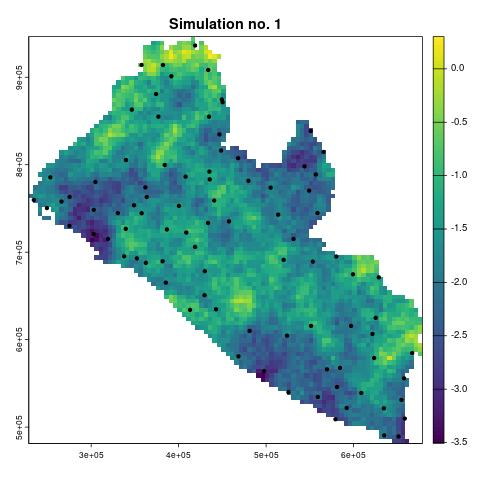
\includegraphics[keepaspectratio]{./figures/sim_surf1.jpeg}}

}

\caption{\label{fig-surf-sim}Simulated surface for the linear predictor,
with locations of the simulated data noted by solid black points.}

\end{figure}%

\subsection{Step 3: Fit the candidate models to the simulated data and
predict the target}\label{sec-sim-step3}

To summarize, the results obtained from Step 1 and Step 2 are as
follows:

\begin{enumerate}
\def\labelenumi{\arabic{enumi}.}
\tightlist
\item
  Simulated values for the linear predictor of the true model (\(M_T\))
  over a grid covering the study area.
\item
  Simulated values for the linear predictor of \(M_T\) at the data
  locations.
\item
  Simulated realizations of the data at the data locations.
\end{enumerate}

Next, we use the third output listed above to fit the candidate models
(\(M_C\)) and make predictions over the grid. Note that each of the
outputs above has been generated \(B\) times, which denotes the number
of simulations.

Using the notation introduced in Section~\ref{sec-spat-cont-target}, let
\(T(x)\) denote the spatially continuous target. When the predictive
target is at the areal level, the necessary adjustments to Step 3 and
Step 4 will be detailed in Section~\ref{sec-sim-assessment}.

The outputs generated in these steps include predictive samples of the
target over the grid, represented by \(T_{(j)}^{(h)}(\tilde{x})\),
where: \(j\) is the index of the \(j\)-th simulated data-set, for
\(j = 1, \ldots, B\); \(h\) is the index of the Monte Carlo samples, for
\(h = 1, \ldots, N\), generated by the Monte Carlo Markov Chain (MCMC)
algorithm for a given data-set \(j\).

An example in R for Step 3 will be provided in the next section, where
we shall use the function \texttt{assess\_sim}, from the
\texttt{RiskMap} package, which combines Step 3 and Step 4 into a single
step.

\subsection{Step 4: Summarize the results using a pre-defined objective
function}\label{step-4-summarize-the-results-using-a-pre-defined-objective-function}

In this final step, we compare the predictions of the target \(T(x)\)
against its true values, originally simulated in Step 1. To do this, we
need a metric to summarize the results across all \(B\) simulations for
each candidate model \(M_C\).

One approach is to use the predictive mean from \(M_C\) in each
simulation and evaluate how it differs from \(T(x)\). A natural choice
for this comparison is the mean squared error (MSE), defined as:

\begin{equation}\phantomsection\label{eq-mse}{
\frac{1}{B} \sum_{j=1}^B \sum_{i=1}^q \left(T(\tilde{x}_i) - \hat{T}_{C}(\tilde{x}_i)\right)^2
}\end{equation}

where \(\tilde{x}_i\) is the \(i\)-th location on the grid
\(\tilde{X}\), \(T(\tilde{x}_i)\) represents the true value of the
target, and \(\hat{T}_{C}(\tilde{x}_i)\) is the predictive mean from
\(M_C\) at location \(\tilde{x}_i\).

Other options for summarizing the results include using the bias or the
absolute median deviation. The bias measures the systematic error
between the predicted and true values and is defined as:

\[
\frac{1}{B} \sum_{j=1}^B \sum_{i=1}^q \left(T(\tilde{x}_i) - \hat{T}_{C}(\tilde{x}_i)\right)
\]

The median absolute deviation (MAD) focuses on the central tendency of
the errors, providing a robust measure of variability. It is defined as:

\[
\text{median}\left(\left|T(\tilde{x}_i) - T^*_{C}(\tilde{x}_i)\right|\right),
\] where \(T^*_{C}(\tilde{x}_i)\) is the median across all \(N\) the
Monte Carlo samples \(T_{(j)}^{(h)}(\tilde{x})\).

\subsubsection{Example}\label{example-2}

Using the output from the \texttt{surf\_sim} function, named
\texttt{lib\_surf\_sim}, we can use as the input to the function
\texttt{assess\_sim} which performs Step 3 and Step 4, previously
outlined.

\begin{Shaded}
\begin{Highlighting}[]
\NormalTok{res\_sim\_grid }\OtherTok{\textless{}{-}} \FunctionTok{assess\_sim}\NormalTok{(lib\_surf\_sim,}
                      \AttributeTok{models =} \FunctionTok{list}\NormalTok{(}\AttributeTok{M\_T =} \SpecialCharTok{\textasciitilde{}}\NormalTok{  elevation }\SpecialCharTok{+}
                                             \FunctionTok{pmax}\NormalTok{(elevation }\SpecialCharTok{{-}} \DecValTok{150}\NormalTok{, }\DecValTok{0}\NormalTok{) }\SpecialCharTok{+}
                                             \FunctionTok{gp}\NormalTok{(long, lat),}
                                    \AttributeTok{M\_C =} \SpecialCharTok{\textasciitilde{}} \FunctionTok{gp}\NormalTok{(long, lat)),}
                      \AttributeTok{f\_grid\_target =} \ControlFlowTok{function}\NormalTok{(x) }\FunctionTok{exp}\NormalTok{(x)}\SpecialCharTok{/}\NormalTok{(}\DecValTok{1}\SpecialCharTok{+}\FunctionTok{exp}\NormalTok{(x)),}
                      \AttributeTok{pred\_objective =} \StringTok{"mse"}\NormalTok{,}
                      \AttributeTok{spatial\_scale =} \StringTok{"grid"}\NormalTok{)}
\end{Highlighting}
\end{Shaded}

In this function, we specify the models to be assessed using the
\texttt{models} argument, which is a list of \texttt{formula} objects.
The formula \texttt{M\_T} represents the true model \(M_T\), while
\texttt{M\_C} corresponds to the intercept-only model. Note that the
coordinate names used in the \texttt{gp()} function within the formulas
are converted according to the CRS specified in \texttt{lib\_suf\_sim}.

The argument \texttt{f\_grid\_target} defines our target function
\(T(x)\) over the grid as a transformation of the linear predictor.
Specifically, \texttt{exp(x)\ /\ (1\ +\ exp(x))} expresses disease
prevalence as our predictive target over the grid. The
\texttt{pred\_objective} argument specifies the objective function from
Step 4, with \texttt{pred\_objective\ =\ "mse"} setting it to the mean
squared error from Equation~\ref{eq-mse}. Finally,
\texttt{spatial\_scle\ =\ "grid"} indicates that the objective function
applies to a pixel-level target according to the grid stored in
\texttt{lib\_surf\_sim}.

We can now look at the summary of \texttt{res\_sim\_grid}.

\begin{Shaded}
\begin{Highlighting}[]
\FunctionTok{summary}\NormalTok{(res\_sim\_grid)}
\end{Highlighting}
\end{Shaded}

\begin{verbatim}
Summary of Simulation Results

Mean Squared Error (MSE):
    Model    MSE_mean       MSE_sd
M_T   M_T 0.004426811 0.0009040507
M_C   M_C 0.004390553 0.0008564500
\end{verbatim}

The results reported here present the average and standard deviation
across 200 simulations for the models \(M_C\) and \(M_T\). The
differences between the two models are negligible, indicating that the
point predictions generated by \(M_C\) and \(M_T\) perform similarly in
recovering the true prevalence surface for river blindness in Liberia.

This result should not be surprising, as estimating regression
relationships with prevalence data can be challenging, potentially
limiting their predictive advantage. However, incorporating covariates
enhances model interpretability, allowing us to understand why the model
makes certain predictions in specific areas, which an intercept-only
model cannot provide. Thus, even if the model with covariates does not
achieve the best predictive performance, we may still choose to retain
the covariates, in this case elevation, for their interpretative value.

\subsection{Assessessment of threshold-based classification of spatial
units using geostatistical models}\label{sec-sim-assessment}

In this section, we address the specific problem of evaluating how
effectively a geostatistical model classifies areal units into
predefined categories of a disease indicator, such as prevalence. This
issue is particularly relevant when dealing with areal-level targets
(Section~\ref{sec-areal-target}) as opposed to spatially continuous
targets (Section~\ref{sec-spat-cont-target}). This prediction problem
arises when policy decisions regarding interventions are often based on
the classification of the areal-level target into predefined categories
at the level of administrative regions; see, for example, Johnson et al.
(2021) and Puranik et al. (2024).

To formalize this problem mathematically, let \(\mathcal{M}_i\)
represent the true value of the areal-level target (e.g., the average
prevalence over a district), and let \(\hat{\mathcal{M}}_{C,i}\) denote
the corresponding prediction produced by the candidate model \(M_C\).
Note that \(\mathcal{M}_i\) can be easily calculated in Step 1 during
simulations from the true model (Section~\ref{sec-sim-step1}).

Now, consider that the target \(\mathcal{M}_i\) is categorized into
predefined classes, which are typically thresholds or ranges of the
disease indicator (such as values that define low, medium, and high
levels). Denote the true membership class of areal unit \(i\) by
\(\mathcal{D}_i\), which is determined based on \(\mathcal{M}_i\), and
the predicted membership class by \(\hat{\mathcal{D}}_{C,i}\),
determined based on \(\hat{\mathcal{M}}_{C,i}\). The goal is to assess
the overall quality of the classification, which involves evaluating how
well the predicted classes \(\hat{\mathcal{D}}_{C,i}\) agree with the
true classes \(\mathcal{C}_i\) across all areal units and simulations.
This assessment provides insight into the model's ability to accurately
classify regions according to the chosen disease indicator and thus
guide effective policy decisions.

The required changes to Step 3 (Section~\ref{sec-sim-step3}) consist of
simply carrying the predictions over the areal units as explained in
Section~\ref{sec-areal-target}.

For Step 4, which concerns how we summarize the agreement between the
classification generated by \(M_C\) and the true classes
\(\mathcal{D}_i\), we can proceed as follows. First, we distinguish
between indicators that can be computed for a given region and those
that summarize performance across all regions.

Assessing classification performance can be approached similarly to
evaluating a diagnostic test. Here, true positives, true negatives,
false positives, and false negatives are defined at the level of
individual spatial units that subdivide the study area. Hence, key
indicators include:

\begin{enumerate}
\def\labelenumi{\arabic{enumi}.}
\item
  \emph{Sensitivity}: The proportion of areal units correctly classified
  as belonging to the true membership class when conditioned on that
  true class:\\
  \[
  \text{Sensitivity} = \frac{\text{True Positives (TP)}}{\text{True Positives (TP)} + \text{False Negatives (FN)}}
  \]
\item
  \emph{Specificity} (True Negative Rate): The proportion of areal units
  not belonging to a given membership class that are correctly
  classified as not being in that class:\\
  \[
  \text{Specificity} = \frac{\text{True Negatives (TN)}}{\text{True Negatives (TN)} + \text{False Positives (FP)}}
  \]
\item
  \emph{Positive Predictive Value (PPV)}: The proportion of areal units
  predicted to belong to a membership class that are correctly
  classified, conditioned on the predicted membership class:\\
  \[
  \text{PPV} = \frac{\text{True Positives (TP)}}{\text{True Positives (TP)} + \text{False Positives (FP)}}
  \]
\item
  \emph{Negative Predictive Value (NPV)}: The proportion of areal units
  predicted not to belong to a membership class that are correctly
  classified, conditioned on the predicted membership class:\\
  \[
  \text{NPV} = \frac{\text{True Negatives (TN)}}{\text{True Negatives (TN)} + \text{False Negatives (FN)}}
  \]
\item
  \emph{Correct Classification Rate}: The overall proportion of areal
  units whose predicted membership class matches the true membership
  class:\\
  \[
  \text{Correct Classification Rate} = \frac{\text{True Positives (TP)} + \text{True Negatives (TN)}}{\text{Total Cases (TP + TN + FP + FN)}}
  \]
\end{enumerate}

Note that for multiple classes, the indicators above are computed by
comparing each class in turn against all other classes combined. This
allows us to create a 2 by 2 table, enabling the calculation of the
indicators above.

The choice between sensitivity, specificity, PPV, and NPV depends on the
specific public health context and the priorities of the decision-making
process. Sensitivity and specificity are conditioned on the \emph{true
membership class}, making them useful for assessing the model's
performance in terms of correctly identifying or excluding true
positives or negatives. PPV and NPV are conditioned on the
\emph{predicted membership class}, making them more informative about
the trustworthiness of predictions, especially when prevalence varies
significantly across regions.

We can thus summarize the difference of each indicator as follows.

\begin{itemize}
\item
  Sensitivity is most appropriate when the priority is to ensure that
  true positive cases (e.g., high-prevalence regions) are not missed.
  Sensitivity is useful in contexts where failing to identify true cases
  could have severe consequences, such as delaying critical
  interventions or underestimating resource needs. For example, during
  an outbreak, ensuring all high-risk areas are flagged is crucial, even
  if this increases the number of false positives.
\item
  Specificity is more suitable when the focus is on minimizing false
  positives, which is critical in contexts where over-classification
  could lead to unnecessary interventions or misallocation of resources.
  Specificity may be particularly important in low-prevalence scenarios,
  where the cost of acting on false alarms could outweigh the benefits
  of capturing all true positives.
\item
  PPV is appropriate when the emphasis is on the reliability of positive
  predictions, i.e., how confident we can be that regions classified as
  high-prevalence are truly high-prevalence. PPV is heavily influenced
  by the prevalence of the condition being classified, making it
  especially relevant in scenarios where actionable decisions depend on
  the certainty of a positive classification.
\item
  NPV is most relevant when it is critical to trust negative
  predictions, i.e., ensuring that regions predicted as low-prevalence
  are indeed low-prevalence. NPV is particularly important in
  low-prevalence settings, where a high proportion of predicted
  negatives are true negatives.
\end{itemize}

Ultimately, the selection of indicators should result from a dialogue
between statisticians, epidemiologists, and policy makers, ensuring
alignment with the specific priorities and policy decisions being
informed by the model's classifications.

\subsubsection{Example}\label{example-3}

Using the same models, \(M_T\) and \(M_C\), from the river blindness
example in Liberia, we now compare their performance in classifying
admin level 1 regions into two prevalence categories, \((0, 0.2)\) and
\$(0.2, 1) \$. The assessment is conducted using \texttt{assess\_sim},
where the prevalence surface is first aggregated at the areal level
before classification.

\begin{Shaded}
\begin{Highlighting}[]
\CommentTok{\# Admin level 1 shape files}
\NormalTok{shp\_adm }\OtherTok{\textless{}{-}} \FunctionTok{geoboundaries}\NormalTok{(}\AttributeTok{country =} \StringTok{"liberia"}\NormalTok{, }\AttributeTok{adm\_lvl =} \StringTok{"adm1"}\NormalTok{)}
\NormalTok{shp\_adm }\OtherTok{\textless{}{-}} \FunctionTok{st\_transform}\NormalTok{(shp\_adm, }\AttributeTok{crs=} \DecValTok{32629}\NormalTok{)}

\NormalTok{res\_sim\_area }\OtherTok{\textless{}{-}} \FunctionTok{assess\_sim}\NormalTok{(lib\_surf\_sim,}
                      \AttributeTok{models =} \FunctionTok{list}\NormalTok{(}\AttributeTok{M\_T =} \SpecialCharTok{\textasciitilde{}}\NormalTok{  elevation }\SpecialCharTok{+}
                                      \FunctionTok{pmax}\NormalTok{(elevation }\SpecialCharTok{{-}} \DecValTok{150}\NormalTok{, }\DecValTok{0}\NormalTok{) }\SpecialCharTok{+}
                                      \FunctionTok{gp}\NormalTok{(long, lat),}
                                    \AttributeTok{M\_C =} \SpecialCharTok{\textasciitilde{}} \FunctionTok{gp}\NormalTok{(long, lat)),}
                      \AttributeTok{f\_grid\_target =} \ControlFlowTok{function}\NormalTok{(x) }\FunctionTok{exp}\NormalTok{(x)}\SpecialCharTok{/}\NormalTok{(}\DecValTok{1}\SpecialCharTok{+}\FunctionTok{exp}\NormalTok{(x)),}
                      \AttributeTok{f\_area\_target =}\NormalTok{ mean,}
                      \AttributeTok{pred\_objective =} \StringTok{"classify"}\NormalTok{, }\AttributeTok{shp =}\NormalTok{ shp\_adm,}
                      \AttributeTok{categories =} \FunctionTok{c}\NormalTok{(}\DecValTok{0}\NormalTok{,}\FloatTok{0.2}\NormalTok{,}\DecValTok{1}\NormalTok{),}
                      \AttributeTok{spatial\_scale =} \StringTok{"area"}\NormalTok{)}
\end{Highlighting}
\end{Shaded}

The implementation first loads the admin level 1 shapefiles for Liberia,
transforming them to the appropriate coordinate reference system. The
arugment \texttt{f\_area\_target} is set to \texttt{mean}, ensuring that
the target prevalence for each region is computed as the average over
the area, corresponding to\\
\[
\frac{1}{|A|} \int_A T(x) \, dx
\] The classification is performed by specifying
\texttt{pred\_objective\ =\ "classify"}, meaning the models are
evaluated based on their ability to assign regions to the correct
prevalence class. The \texttt{categories} argument defines the
classification thresholds, requiring at least three values to
distinguish between two classes. The \texttt{spatial\_scale} is set to
\texttt{"area"}, meaning predictions are made at the level of
administrative regions which are specified by the shapefile
\texttt{shp\_adm}, passed to the argument \texttt{shp}.

Finally, we can examine the results of the simulation through the
summary function.

\begin{Shaded}
\begin{Highlighting}[]
\FunctionTok{summary}\NormalTok{(res\_sim\_area)}
\end{Highlighting}
\end{Shaded}

\begin{verbatim}
Summary of Simulation Results

Classification Results:

Model: M_T

Averages across simulations by Category:
  Sensitivity Specificity       PPV       NPV        CC   Class
1   0.9020851   0.8151707 0.8923583 0.8654312 0.9020851 (0,0.2]
2   0.8151707   0.9020851 0.8654312 0.8923583 0.8151707 (0.2,1]

Proportion of Correct Classification (CC) across categories:
Mean: 0.871, 95% CI: [0.665, 1.000]

Model: M_C

Averages across simulations by Category:
  Sensitivity Specificity       PPV       NPV        CC   Class
1   0.9048404   0.7974989 0.8890838 0.8581346 0.9048404 (0,0.2]
2   0.7974989   0.9048404 0.8581346 0.8890838 0.7974989 (0.2,1]

Proportion of Correct Classification (CC) across categories:
Mean: 0.868, 95% CI: [0.600, 1.000]
\end{verbatim}

In this example, the performance of models \(M_T\)\hspace{0pt} and
\(M_C\)\hspace{0pt} is comparable across all considered indicators. This
similarity arises for the same reasons previously discussed examining
the quality of prevalence surface predictions.

\section{Theory}\label{sec-theory-prediction}

\subsection{Expression of the predictive distribution for a linear
geostatistical model}\label{sec-pred-distr-theory}

In this section, we consider the simple case of a linear geostatistical
model with a single observation per location.

Let \(Y = (Y_1, \ldots, Y_n)^\top\) be the vector of data associated
with spatial locations \(x_1, \ldots, x_n\). The model assumes that:

\begin{equation}
Y_i = d(x_i)^\top {\beta} + S(x_i) + Z_i, \quad i = 1, \ldots, n,
\end{equation}

where \(d(x_i)\) is a vector of covariates at location \(x_i\),
\({\beta}\) is a vector of regression coefficients, \(S(x)\) is a
stationary Gaussian process with mean zero and Matern correlation
function \(\rho(u)\) (where \(u\) is the distance between locations),
and \(Z_i \sim \mathcal{N}(0, \tau^2)\) represents independent
measurement errors (nugget effect).

We first consider the simple case of a linear target, hence
\(T(x) = d(x)^\top {\beta} + S(x)\). The goal is to predict the
unobserved process \(T^* = (T_{n+1}, \ldots, T_{n+q})^\top\) at new
locations \(x_{n+1}, \ldots, x_{n+q}\). The predictive distribution of
\(T^*\), conditional on the observed data \(Y\), follows a multivariate
Gaussian distribution:

\begin{equation}
T^* | Y \sim \mathcal{N}(\mu^*, \Sigma^*),
\end{equation}

where the conditional mean and covariance are given by:

\begin{align}
\mu^* &= D^* {\beta} + C \Sigma^{-1} (Y - D {\beta}), \\
{\Sigma}^* &= V - C \Sigma^{-1} C^\top.
\end{align}

Here, \(D^*\) is the design matrix for the prediction locations, \(C\)
is the cross-covariance matrix between \(T^*\) and \(Y\), \(\Sigma\) is
the covariance matrix of \(Y\), and \(V\) is the covariance matrix of
\(T^*\). Using a multivariate Gaussian distribution with mean \(\mu^*\)
and covariance matrix \(\Sigma^*\), we are now able to predict \(T^*\)
and obtain summaries of uncertainties.

For non-linear prediction targets, i.e.~targets that involve non-linear
transformations of the spatial process \(S(x)\), say \(W(T^*)\), Monte
Carlo methods can be employed. More specifically, we generate samples
\(T_{(j)}^*\), for \(j=1,\ldots,B\) from the predictive distribution
\(T^* | Y\) using the multivariate Gaussian distribution with mean
\(\boldsymbol{\mu}^*\) and covariance \(\boldsymbol{\Sigma}^*\). For
each sample \(T^{*}_{(j)}\), the non-linear transformation
\(W(T^{*}_{(j)} = W^{*}_{(j)}\) of interest is then computed. The
predictive summary statistics, such as the mean, variance, or quantiles
of \(W(T^*)\), are then estimated by averaging over the simulated
samples, e.g.

\begin{align}
E[W(T^*) | Y] &\approx  \frac{1}{B} \sum_{J=1}^B W^{*}_{(j)}), \\
\text{Var}[W(T^*) | Y] &\approx \frac{1}{B-1} \sum_{j=1}^B \left( W^{*}_{(j)} - E[W(T^*)] \right)^2.
\end{align}

For more detailed explanations on this we refer you to Chapter 6 of P.
Diggle and Ribeiro (2007).

\subsection{A brief overview of scoring
rules}\label{a-brief-overview-of-scoring-rules}

We now provide an overview of the theoretical framework of \emph{scoring
rules}, of which the continuous ranked probability score (CRPS) and its
scaled variant (SCRPS), previously presented, are an example. Scoring
rules are a tool used in the evaluation of probabilistic forecasts. As
shown for CRPS and SCRPS, scoring rules are designed to measure how well
a predictive distribution aligns with observed outcomes, balancing both
\emph{calibration} and \emph{sharpness}.

In general, a scoring rule is a function \(G(F, y)\) that assigns a
numerical score to a predictive distribution \(F\) and an observed
outcome \(y\). Lower scores typically indicate better predictive
performance, as they reflect a closer match between the predicted
distribution and the observed value.

A central concept in the theory of scoring rules is that of \emph{proper
scoring rules}. A scoring rule is said to be \emph{proper} if it favours
honest predictions or, in other words, if the expected score is
minimized when the predictive distribution \(F\) matches the true
data-generating distribution \(F^*\). More formally, a scoring rule
\(G\) is proper if, for all distributions \(F\) and \(F^*\), we have: \[
E_{Y \sim F^*}[G(F^*, Y)] \leq E_{Y \sim F^*}[G(F, Y)],
\] with equality if and only if \(F = F^*\) when the rule is
\emph{strictly proper}. This property is crucial because it ensures that
forecasters cannot improve their scores by manipulating their
predictions to deviate from their true beliefs.

Proper scoring rules encourage the selection of models that yield
predictions that are both well-calibrated (reflecting the true
distribution of outcomes) and sharp (concentrated around likely values).
However, this does not imply that predictions from the (unknown) true
model \(F^*\) will always be favoured in practice, when dealing with
finite samples. In other words, even if two scoring rules are proper,
this does not guarantee that the true data-generating model will always
achieve a lower score compared to a misspecified model in finite
samples. \emph{Sample variability} can in fact lead to the selection of
a misspecified model by chance, especially when the sample size is small
or the data are noisy. \emph{Model complexity} is another important
factor. If the true model \(F^*\) is highly parameterised and the sample
size is insufficient to estimate its parameters accurately, it may
perform poorly in predictive tasks due to overfitting or parameter
estimation error. In contrast, a simpler misspecified model, despite not
capturing the full complexity of the data-generating process, might
generalize better in such scenarios. This is related to the
bias-variance trade-off, where a model with higher bias (due to
misspecification) can still achieve lower overall predictive error if it
has substantially lower variance.

The CRPS and SCRPS are examples of a strictly proper scoring rule for
continuous outcomes. Other scoring rules are the following:

\begin{itemize}
\item
  \emph{Logarithmic Score (or Log Score):} For a predictive density
  \(f(y)\), the log score is defined as: \[
  G_{\text{log}}(f, y) = -\log f(y).
  \] This rule heavily penalizes low-probability predictions for
  observed outcomes, making it sensitive to the tails of the predictive
  distribution.
\item
  \emph{Brier Score:} For binary outcomes, the Brier score measures the
  mean squared difference between the predicted probability \(p\) of an
  event and the actual outcome \(y \in \{0, 1\}\): \[
  G_{\text{Brier}}(p, y) = (p - y)^2.
  \] The Brier score is both proper and easy to interpret, with
  connections to mean squared error in classical regression.
\item
  \emph{Energy Score:} A generalization of the CRPS to multivariate
  outcomes, the energy score for a predictive distribution \(F\) and
  observation \(y\) is given by: \[
  G_{\text{energy}}(F, y) = E_{X, X' \sim F}[\|X - X'\|] - 2 E_{X \sim F}[\|X - y\|],
  \] where \(\|\cdot\|\) denotes a norm, typically the Euclidean norm.
  The energy score is particularly useful for evaluating spatial or
  multivariate forecasts.
\end{itemize}

Many proper scoring rules, including the CRPS, can be decomposed into
components that separately capture calibration and sharpness. This
decomposition helps to understand the different aspects of predictive
performance. Specifically, the expected score can often be expressed as:
\[
E[G(F, Y)] = \underbrace{\text{Uncertainty}}_{\text{inherent in data}} - \underbrace{\text{Resolution}}_{\text{sharpness of predictions}} + \underbrace{\text{Reliability}}_{\text{calibration error}},
\] where: - \emph{Uncertainty} represents the inherent variability in
the data, independent of the model. - \emph{Resolution} quantifies the
model's ability to produce sharp, confident forecasts. -
\emph{Reliability} (or calibration error) measures the degree to which
the forecast probabilities align with observed frequencies.

This decomposition highlights an important trade-off: improving
sharpness without compromising calibration is the hallmark of a good
probabilistic model. A model that produces overly sharp forecasts may
suffer from poor calibration, while a model that is perfectly calibrated
but overly diffuse lacks resolution.

As we have shown in this chapter, scoring rules are particularly
appropriate in cross-validation frameworks, where the goal is to
evaluate how well a model predicts future data realizations. When
instead conducting simulation studies, we generate data from a known
simulated true surface which becomes our benchmark. Hence, in simulation
studies, we do not perform cross-validation but, for a given simulation,
we compare the model predictions against the true surface. In such
cases, scoring rules are not used because they are designed to assess
predictive performance based on observed data, where both calibration
and sharpness are critical considerations. Hence, in simulation studies,
prediction performance metrics, such as bias, mean squared error (MSE),
or other distance-based metrics that directly quantify the deviation
from the known truth can be used to quantify the predictive performance
of a model.

For a more detailed explanation of scoring rules, Gneiting, Balabdaoui,
and Raftery (2007) is a recommended read.

\section{Summary}\label{summary}

In this chapter, we have demonstrated how geostatistical models can be
used to draw predictive inference for targets that are spatially
continuous (e.g., a prevalence surface within a study region) and
aggregated at the areal level (e.g., the average disease prevalence in a
district). The fundamental concept underpinning geostatistical
prediction is that of the \textbf{predictive distribution}, which we
define as the distribution of the target \(T(x)\) conditioned on the
data \(y\). This distribution is the key element that enables the
derivation and computation of point predictions, predictive intervals
and the probability that the target falls within a pre-specified
interval or above/below a given threshold.

To assess the predictive performance of a geostatistical model, we have
considered two complementary approaches: \textbf{cross-validation} and
\textbf{simulation studies}.

In the cross-validation framework, the concepts of \textbf{calibration}
and \textbf{sharpness} are introduced to evaluate the quality of spatial
predictions. Calibration refers to the agreement between the predicted
probability of an event occurring and its actual observed frequency.
Sharpness, on the other hand, quantifies the concentration of the
predictive distribution around its point estimate. However, sharper
predictions are not necessarily better; they must be well-calibrated to
be meaningful. Thus, it is appropriate to discuss sharpness only in the
context of well calibrated models.

A simulation study, unlike cross-validation, allows us to assess the
ability of our model to predict an entire spatial surface within a study
area or a predictive target defined over spatial units (e.g., districts)
that make up the study area. This is possible because, in a simulation
study, we can generate data from a \textbf{true model} and then evaluate
the quality of inferences from \textbf{candidate models} on the
simulated surface. The way we summarize predictive performance in a
simulation study depends on the objective. If the goal is to assess how
closely our point predictions align with the true surface, we can use
metrics such as the mean squared error (Equation~\ref{eq-mse}), averaged
over the grid used to approximate the surface. Conversely, if the
objective is to evaluate classification performance by categorizing
spatial units into predefined health outcome categories, we can use
sensitivity, specificity, negative predictive value, and positive
predictive value. The choice of metric depends on whether the priority
is minimizing errors in detecting true positives or true negatives
(sensitivity and specificity), or ensuring that the spatial units
classified as positive or negative are truly so (positive predictive
value and negative predictive value). A summary of the metrics
considered in this chapter is given in Table~\ref{tbl-summary-pp-diag}.

\begin{longtable}[]{@{}
  >{\raggedright\arraybackslash}p{(\linewidth - 4\tabcolsep) * \real{0.4167}}
  >{\raggedright\arraybackslash}p{(\linewidth - 4\tabcolsep) * \real{0.3056}}
  >{\raggedright\arraybackslash}p{(\linewidth - 4\tabcolsep) * \real{0.2778}}@{}}
\caption{Summary of the different diagnostic tools and metrics, that are
used to assess the predictive performance of a geostatistical model
using both cross-validation and simulatoin-based
approaches.}\label{tbl-summary-pp-diag}\tabularnewline
\toprule\noalign{}
\begin{minipage}[b]{\linewidth}\raggedright
Diagnostic/Metric
\end{minipage} & \begin{minipage}[b]{\linewidth}\raggedright
Performance characteristic
\end{minipage} & \begin{minipage}[b]{\linewidth}\raggedright
Recommended use in
\end{minipage} \\
\midrule\noalign{}
\endfirsthead
\toprule\noalign{}
\begin{minipage}[b]{\linewidth}\raggedright
Diagnostic/Metric
\end{minipage} & \begin{minipage}[b]{\linewidth}\raggedright
Performance characteristic
\end{minipage} & \begin{minipage}[b]{\linewidth}\raggedright
Recommended use in
\end{minipage} \\
\midrule\noalign{}
\endhead
\bottomrule\noalign{}
\endlastfoot
Bias & Accuracy & Simulation \\
Continuous ranked probability score (CRPS) & Calibration and sharpness &
Cross-validation \\
Coverage probability & Calibration & Cross-validation and simulation \\
Mean square error & Accuracy & Simulation \\
Nonrandomized probability integral transform (PIT) & Calibration &
Cross-validation \\
PIT & Calibration & Cross-validation \\
Scaled CRPS & Calibration and sharpness & Cross-validation \\
\end{longtable}

\section{FAQs}\label{faqs}

\begin{itemize}
\tightlist
\item
  \emph{What should be the spatial resolution of the grid used for
  prediction?}
\end{itemize}

The choice of spatial resolution for the prediction grid involves a
trade-off between computational efficiency and the ability to capture
spatial correlation. Higher spatial resolution provides more detailed
predictions but increases computational demands. A reasonable approach
is to ensure that the distance between adjacent grid pixels is small
enough to maintain a high spatial correlation. For instance, selecting a
resolution where the correlation between neighboring pixels is at least
0.95 can be a useful guideline. However, this threshold is somewhat
arbitrary, similar to the convention of using 0.95 in confidence
intervals. Ultimately, the resolution should be chosen based on the
spatial scale of variation in the data, while avoiding excessive
computational burden.

\begin{itemize}
\tightlist
\item
  \emph{I have covariates with different spatial resolutions. Which
  spatial resolution should I use?}
\end{itemize}

Two main approaches can be considered for handling covariates at
different spatial resolutions in geostatistical analysis. The first
involves aggregating all covariates to the coarsest resolution, ensuring
consistency and avoiding artificial detail. This prevents
high-resolution predictions based on low-resolution data but may
sacrifice fine-scale spatial variation. The second approach
disaggregates covariates to the finest resolution, enabling
higher-detail predictions but risking false precision and artifacts if
the data do not support such resolution. To assess the impact on
inferences, one might apply both approaches and evaluate how they
influence the final results.

\begin{itemize}
\tightlist
\item
  \emph{My prediction map looks like noise. What could be the error?}
\end{itemize}

The prediction map appearing noisy could be due to several factors.
First, one should verify that the spatial grid was created correctly by
plotting it alongside the original data to ensure alignment and
consistency. Second, the spatial correlation in the data might be very
small relative to the resolution of the grid, causing the model to
struggle with capturing meaningful patterns. To address this, increasing
the spatial resolution of the grid may help, as finer resolution can
better capture the underlying spatial structure.

\begin{itemize}
\tightlist
\item
  \emph{The main goal of my analysis is to carry out predictions of the
  main outcome. However, can I also use the model to draw inferences on
  the association between the outcome and the covariates that I have
  included in the model?}
\end{itemize}

The model developed for prediction, in theory, should not be primarily
used to draw inferences on the regression relationships between the
outcome and covariates. Understanding regression relationships and
making predictions are distinct goals that often require different
modeling approaches. While it is possible to interpret the estimated
regression coefficients, caution is necessary, as these associations are
not causative. Predictive models are optimized for accuracy in
predicting th outcome rather than for identifying or explaining
underlying relationships, so any inferences drawn should be treated as
exploratory rather than definitive. An recommended reading on this topic
is Shmueli (2010).

\begin{itemize}
\tightlist
\item
  \emph{In my model I have some covariates that are attached to the
  individual (e.g.~age, gender, occupation, etc.). How do I specify them
  when doing prediction?}
\end{itemize}

The answer to this question is given in
Section~\ref{sec-non-spar-covariates}.

\section{Review questions}\label{review-questions-2}

\begin{itemize}
\tightlist
\item
  What are the steps that needs to taken when performing spatial
  prediction?
\item
  Define the predictive distribution of a predictive target and explain
  how this is used to answer a research question.
\item
  Distinguish between spatially continuous and areal-level targets,
  giving at least two examples for each.
\item
  Explain the difference between marginal and joint predictions, and for
  which targets each can be used.
\item
  Define predictive performance in terms of calibration and sharpness.
\item
  Explain how calibration can be assessed using graphical tools, by
  distinguishing between continuous and count outcomes.
\item
  Give examples of metrics that can be used to evaluate calibration and
  sharpness.
\item
  Explain how simulation studies can be carried to assess the predictive
  performance of geostatistical models and how this differ from
  cross-validation.
\end{itemize}

\section{Exercises}\label{exercises-2}

\begin{enumerate}
\def\labelenumi{\arabic{enumi}.}
\item
  Using the code from Section~\ref{sec-compare-pp}, redraw the plot of
  Figure~\ref{fig-anpit} by choosing different values for the dispersion
  parameter of the Negative Binomial distribution. What happens when
  \(\alpha\) is close to 0 and why?
\item
  Consider the example in Section~\ref{sec-liberia-anpit}. Fit a third
  model, that extends \(M1\) by adding a nugget effect, hence \[
  M_{2} \: : \: \log\left\{\frac{p(x_i)}{1-p(x_i)}\right\} = \beta_0 + \beta_{1}e(x_i) + \beta_{2}\max\{e(x_i) - 150, 0\} + S(x_i) + Z_i.
  \] Generate the AnPIT plot for \(M_2\) and compare it to those of
  \(M_0\) and \(M_1\). Make sure to apply the function
  \texttt{assess\_pp} to all three models so that the same test sets are
  used. Is \(M_2\) showing a better calibration? Why?
\item
  In the analysis of the \emph{Anopheles gambiae} moqsuitoes data,
  consider two models. One that uses elavation, with linear predictor \[
  M_1\: : \: \log\{\lambda(x_i)\} = \beta_0 + \beta_1 e(x_i) + S(x_i)
  \] where \(e(x)\) is the elevation in meters at location \(x\) and
  \(S(x_i)\) is a stationary and isotropic Gaussian process with
  variance \(\sigma^2\) and exponential correlation function
  \(\rho(u) = \exp\{-u/\phi\}, \phi>0\). Consider also an intercept only
  model \[
  M_0\: : \: \log\{\lambda(x_i)\} = \beta_0 +  S(x_i).
  \] After fitting both models to the data, assess if they are well
  calibrated models using the average nonrandomized probability integral
  transform (AnPIT). Assuming both models are well-calibrated, compare
  the predictive performance using continuous ranked probability score
  (CRPS) and the scaled CRPS. In doing this, use different sampling
  schemes to split the data, as illustrated in
  Section~\ref{sec-split-data}, and assess if and how the adopted
  approach to split the data affects the results.
\item
  Consider the Liberia data-set on riverblindess. Carry out a simulation
  study where the objective is to assess the impact of mispecifying
  non-linear relationships between elevation and prevalence. Consider
  Equation~\ref{eq-true-model-lib} as the true model and a model that
  specifies the relationship as linear on the logit scale as the
  candidate model, hence \[M_{C}: \:
  \log\left\{\frac{p(x_i)}{1-p(x_i)}\right\} = \beta_{0} + \beta_{1}e(x_i) + S(x_i).
  \] Carry out 200 iterations in the simulation and define a suitable
  metric of predictive performance to compare the two models. Provide a
  clear answer on the impact of assuming a linear relationship with
  elevation when this is not valid.
\end{enumerate}

\bookmarksetup{startatroot}

\chapter{Case studies}\label{sec-case-studies}

In this chapter, we bring together the concepts introduced in the
previous chapters, ranging from exploratory analysis to spatial
prediction, through a series of case studies. Each case study provides a
complete workflow, showing how the different stages of a geostatistical
analysis fit together in practice. Some of these case studies are
designed primarily to consolidate earlier material, while others also
introduce new concepts and additional functionalities of the
\texttt{RiskMap} package that extend beyond the basics.

\section{Mapping stunting and underwieght risk in
Ghana}\label{sec-ghana}

Malnutrition remains a critical public health issue in many low- and
middle-income countries, particularly affecting children under five
years of age. It can have long-term consequences on physical growth,
cognitive development, and susceptibility to disease. Monitoring
childhood nutritional status is essential for evaluating the
effectiveness of health interventions and informing policy decisions.

Two widely used anthropometric indicators derived from child growth
measurements are:

\begin{itemize}
\item
  Height-for-Age Z-score (HAZ): A measure of stunting, which reflects
  chronic malnutrition. Children with a HAZ below -2 standard deviations
  from the WHO growth reference median are considered stunted,
  indicating long-term nutritional deprivation or repeated infections.
\item
  Weight-for-Age Z-score (WAZ): A composite indicator of underweight,
  capturing both acute and chronic malnutrition. Children with WAZ below
  -2 are considered underweight. This measure is commonly used in
  population-based surveys because it is relatively easy to collect and
  interpret.
\end{itemize}

These Z-scores are calculated by comparing individual anthropometric
measurements to the WHO Child Growth Standards, which were developed
based on data from healthy children under optimal environmental and
nutritional conditions (WHO 2006).

Geostatistical models applied to HAZ and WAZ, or to the prevalence of
stunting and underweight derived from these scores, can help answer
critical questions such as: \emph{Where is the burden of malnutrition
highest? How does it relate to socioeconomic or environmental factors?
And which areas should be prioritized for targeted nutritional
interventions?}

In this case study, we analyse HAZ and WAZ as continuous outcomes to
assess the spatial variation in child malnutrition across Ghana and its
association with socioeconomic and demographic covariates.

\subsection{Exploratory analysis}\label{exploratory-analysis-1}

We begin by loading the necessary R packages and the
\texttt{malnutrition} dataset. This geostatistical dataset is derived
from the 2014 Ghana Demographic and Health Survey (DHS) (Ghana
Statistical Service, Ghana Health Service, and ICF International 2015),
which provides nationally representative data on child health and
nutrition. The dataset includes anthropometric measurements, household
characteristics, and georeferenced sampling cluster coordinates, making
it suitable for spatial analysis of child malnutrition.

\begin{Shaded}
\begin{Highlighting}[]
\CommentTok{\# Load packages}
\FunctionTok{library}\NormalTok{(RiskMap)}
\FunctionTok{library}\NormalTok{(ggplot2)}
\FunctionTok{library}\NormalTok{(dplyr)}
\FunctionTok{library}\NormalTok{(patchwork)}

\CommentTok{\# Load the data}
\FunctionTok{data}\NormalTok{(malnutrition)}
\end{Highlighting}
\end{Shaded}

The explanatory variables considered in this analysis are \texttt{age}
and \texttt{wealth}. Figure Figure~\ref{fig-maln-expl} displays
scatterplots of the two nutritional outcomes (\texttt{HAZ} and
\texttt{WAZ}) against age, alongside boxplots stratified by the three
levels of the \texttt{wealth} variable.

To explore the relationship between age and nutritional status, the code
below applies locally estimated scatterplot smoothing (LOESS) to
highlight potential non-linear trends. In addition, we fit linear
splines using the function \texttt{pmax()} to model a change in slope at
specified knots---2 months for HAZ and 1 month for WAZ. These change
points were selected heuristically based on visual inspection of the
LOESS curves.

As shown in Figure Figure~\ref{fig-maln-expl}, the linear splines (green
dashed lines) closely follow the LOESS fits (solid red lines),
indicating that the piecewise linear models provide an adequate
approximation of the age-nutrition relationship.

\begin{Shaded}
\begin{Highlighting}[]
\CommentTok{\# Filter complete cases for relevant variables}
\NormalTok{mal }\OtherTok{\textless{}{-}}\NormalTok{ malnutrition }\SpecialCharTok{\%\textgreater{}\%}
  \FunctionTok{filter}\NormalTok{(}\SpecialCharTok{!}\FunctionTok{is.na}\NormalTok{(HAZ), }\SpecialCharTok{!}\FunctionTok{is.na}\NormalTok{(WAZ), }\SpecialCharTok{!}\FunctionTok{is.na}\NormalTok{(age), }\SpecialCharTok{!}\FunctionTok{is.na}\NormalTok{(wealth))}

\CommentTok{\# Fit spline model for HAZ with knot at 2 months}
\NormalTok{mod\_haz }\OtherTok{\textless{}{-}} \FunctionTok{lm}\NormalTok{(HAZ }\SpecialCharTok{\textasciitilde{}}\NormalTok{ age }\SpecialCharTok{+} \FunctionTok{pmax}\NormalTok{(age }\SpecialCharTok{{-}} \DecValTok{2}\NormalTok{, }\DecValTok{0}\NormalTok{), }\AttributeTok{data =}\NormalTok{ mal)}

\CommentTok{\# Fit spline model for WAZ with knot at 1 month}
\NormalTok{mod\_waz }\OtherTok{\textless{}{-}} \FunctionTok{lm}\NormalTok{(WAZ }\SpecialCharTok{\textasciitilde{}}\NormalTok{ age }\SpecialCharTok{+} \FunctionTok{pmax}\NormalTok{(age }\SpecialCharTok{{-}} \DecValTok{1}\NormalTok{, }\DecValTok{0}\NormalTok{), }\AttributeTok{data =}\NormalTok{ mal)}

\CommentTok{\# Prediction grid for HAZ}
\NormalTok{newdat\_haz }\OtherTok{\textless{}{-}} \FunctionTok{data.frame}\NormalTok{(}\AttributeTok{age =} \FunctionTok{seq}\NormalTok{(}\FunctionTok{min}\NormalTok{(mal}\SpecialCharTok{$}\NormalTok{age), }\FunctionTok{max}\NormalTok{(mal}\SpecialCharTok{$}\NormalTok{age), }\AttributeTok{length.out =} \DecValTok{200}\NormalTok{)) }
\NormalTok{newdat\_haz}\SpecialCharTok{$}\NormalTok{fit }\OtherTok{\textless{}{-}} \FunctionTok{predict}\NormalTok{(mod\_haz, }\AttributeTok{newdata =}\NormalTok{ newdat\_haz)}

\CommentTok{\# Prediction grid for WAZ}
\NormalTok{newdat\_waz }\OtherTok{\textless{}{-}} \FunctionTok{data.frame}\NormalTok{(}\AttributeTok{age =} \FunctionTok{seq}\NormalTok{(}\FunctionTok{min}\NormalTok{(mal}\SpecialCharTok{$}\NormalTok{age), }\FunctionTok{max}\NormalTok{(mal}\SpecialCharTok{$}\NormalTok{age), }\AttributeTok{length.out =} \DecValTok{200}\NormalTok{)) }
\NormalTok{newdat\_waz}\SpecialCharTok{$}\NormalTok{fit }\OtherTok{\textless{}{-}} \FunctionTok{predict}\NormalTok{(mod\_waz, }\AttributeTok{newdata =}\NormalTok{ newdat\_waz)}

\CommentTok{\# Plot HAZ vs Age}
\NormalTok{p1 }\OtherTok{\textless{}{-}} \FunctionTok{ggplot}\NormalTok{(mal, }\FunctionTok{aes}\NormalTok{(}\AttributeTok{x =}\NormalTok{ age, }\AttributeTok{y =}\NormalTok{ HAZ)) }\SpecialCharTok{+}
  \FunctionTok{geom\_point}\NormalTok{(}\AttributeTok{alpha =} \FloatTok{0.3}\NormalTok{) }\SpecialCharTok{+}
  \FunctionTok{geom\_smooth}\NormalTok{(}\AttributeTok{method =} \StringTok{"loess"}\NormalTok{, }\AttributeTok{colour =} \StringTok{"red"}\NormalTok{, }\AttributeTok{se =} \ConstantTok{FALSE}\NormalTok{) }\SpecialCharTok{+}
  \FunctionTok{geom\_line}\NormalTok{(}\AttributeTok{data =}\NormalTok{ newdat\_haz, }\FunctionTok{aes}\NormalTok{(}\AttributeTok{x =}\NormalTok{ age, }\AttributeTok{y =}\NormalTok{ fit), }
            \AttributeTok{colour =} \StringTok{"green"}\NormalTok{, }\AttributeTok{linetype =} \StringTok{"dashed"}\NormalTok{, }\AttributeTok{linewidth =} \FloatTok{1.2}\NormalTok{) }\SpecialCharTok{+}
  \FunctionTok{labs}\NormalTok{(}\AttributeTok{title =} \StringTok{"HAZ vs Age"}\NormalTok{, }\AttributeTok{x =} \StringTok{"Age (months)"}\NormalTok{, }\AttributeTok{y =} \StringTok{"HAZ"}\NormalTok{) }\SpecialCharTok{+}
  \FunctionTok{theme\_minimal}\NormalTok{()}

\CommentTok{\# Plot WAZ vs Age}
\NormalTok{p2 }\OtherTok{\textless{}{-}} \FunctionTok{ggplot}\NormalTok{(mal, }\FunctionTok{aes}\NormalTok{(}\AttributeTok{x =}\NormalTok{ age, }\AttributeTok{y =}\NormalTok{ WAZ)) }\SpecialCharTok{+}
  \FunctionTok{geom\_point}\NormalTok{(}\AttributeTok{alpha =} \FloatTok{0.3}\NormalTok{) }\SpecialCharTok{+}
  \FunctionTok{geom\_smooth}\NormalTok{(}\AttributeTok{method =} \StringTok{"loess"}\NormalTok{, }\AttributeTok{colour =} \StringTok{"red"}\NormalTok{, }\AttributeTok{se =} \ConstantTok{FALSE}\NormalTok{) }\SpecialCharTok{+}
  \FunctionTok{geom\_line}\NormalTok{(}\AttributeTok{data =}\NormalTok{ newdat\_waz, }\FunctionTok{aes}\NormalTok{(}\AttributeTok{x =}\NormalTok{ age, }\AttributeTok{y =}\NormalTok{ fit), }
            \AttributeTok{colour =} \StringTok{"green"}\NormalTok{, }\AttributeTok{linetype =} \StringTok{"dashed"}\NormalTok{, }\AttributeTok{linewidth =} \FloatTok{1.2}\NormalTok{) }\SpecialCharTok{+}
  \FunctionTok{labs}\NormalTok{(}\AttributeTok{title =} \StringTok{"WAZ vs Age"}\NormalTok{, }\AttributeTok{x =} \StringTok{"Age (months)"}\NormalTok{, }\AttributeTok{y =} \StringTok{"WAZ"}\NormalTok{) }\SpecialCharTok{+}
  \FunctionTok{theme\_minimal}\NormalTok{()}

\CommentTok{\# Boxplots for HAZ and WAZ by wealth}
\NormalTok{p3 }\OtherTok{\textless{}{-}} \FunctionTok{ggplot}\NormalTok{(mal, }\FunctionTok{aes}\NormalTok{(}\AttributeTok{x =} \FunctionTok{factor}\NormalTok{(wealth), }\AttributeTok{y =}\NormalTok{ HAZ)) }\SpecialCharTok{+}
  \FunctionTok{geom\_boxplot}\NormalTok{(}\AttributeTok{fill =} \StringTok{"lightblue"}\NormalTok{) }\SpecialCharTok{+}
  \FunctionTok{labs}\NormalTok{(}\AttributeTok{title =} \StringTok{"HAZ by Wealth Group"}\NormalTok{, }\AttributeTok{x =} \StringTok{"Wealth (1 = Poor, 3 = Rich)"}\NormalTok{, }\AttributeTok{y =} \StringTok{"HAZ"}\NormalTok{) }\SpecialCharTok{+}
  \FunctionTok{theme\_minimal}\NormalTok{()}

\NormalTok{p4 }\OtherTok{\textless{}{-}} \FunctionTok{ggplot}\NormalTok{(mal, }\FunctionTok{aes}\NormalTok{(}\AttributeTok{x =} \FunctionTok{factor}\NormalTok{(wealth), }\AttributeTok{y =}\NormalTok{ WAZ)) }\SpecialCharTok{+}
  \FunctionTok{geom\_boxplot}\NormalTok{(}\AttributeTok{fill =} \StringTok{"lightgreen"}\NormalTok{) }\SpecialCharTok{+}
  \FunctionTok{labs}\NormalTok{(}\AttributeTok{title =} \StringTok{"WAZ by Wealth Group"}\NormalTok{, }\AttributeTok{x =} \StringTok{"Wealth (1 = Poor, 3 = Rich)"}\NormalTok{, }\AttributeTok{y =} \StringTok{"WAZ"}\NormalTok{) }\SpecialCharTok{+}
  \FunctionTok{theme\_minimal}\NormalTok{()}

\CommentTok{\# Combine plots}
\NormalTok{(p1 }\SpecialCharTok{|}\NormalTok{ p2) }\SpecialCharTok{/}\NormalTok{ (p3 }\SpecialCharTok{|}\NormalTok{ p4)}
\end{Highlighting}
\end{Shaded}

\begin{figure}[H]

\centering{

\pandocbounded{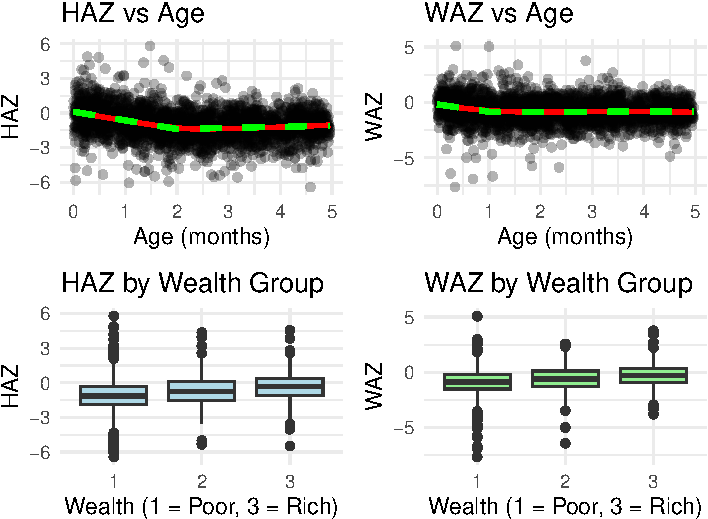
\includegraphics[keepaspectratio]{05_case-studies_files/figure-pdf/fig-maln-expl-1.pdf}}

}

\caption{\label{fig-maln-expl}Exploratory analysis of HAZ and WAZ by age
and wealth. The red lines correspond to LOESS smoothed curves and the
green lines to linear splines with change points at 2 months (HAZ) and 1
month (WAZ) of age. Boxplots show variation by household wealth group.}

\end{figure}%

We begin by fitting a non-spatial model to assess whether there is
residual spatial correlation that remains after accounting for the
effects of age and wealth. Let \(Y_{ij}\) represent either the HAZ or
WAZ score for the \(j\)-th child in the \(i\)-th cluster. The model
takes the following form:

\begin{equation}\phantomsection\label{eq-model-haz-waz}{
Y_{ij} = \beta_0 + \beta_1 a_{ij} + \beta_2 \max\{a_{ij} - c, 0\} + \beta_3 w_i + Z_i + U_{ij},
}\end{equation}

where \(a_{ij}\) denotes the age in months of child \(j\) in cluster
\(i\), and \(w_i\) is the wealth score associated with cluster \(i\); as
previously stated, the change point \(c\) of the linear spline is set to
2 months for HAZ and 1 month for WAZ. The term \(Z_i\) is a Gaussian
random effect with mean zero and variance \(\tau^2\), capturing
between-cluster variation not explained by the covariates. The error
term \(U_{ij}\) represents child-specific residual variation and is
assumed to be Gaussian with mean zero and variance \(\omega^2\).

To fit this model, we create a cluster ID variable based on the sampling
coordinates and include it as a random intercept in the \texttt{lmer}
function to incorporate the term \(Z_i\).

\begin{Shaded}
\begin{Highlighting}[]
\CommentTok{\# Create ID for the location}
\NormalTok{malnutrition }\OtherTok{\textless{}{-}}\NormalTok{ malnutrition }\SpecialCharTok{\%\textgreater{}\%}
  \FunctionTok{group\_by}\NormalTok{(lng, lat) }\SpecialCharTok{\%\textgreater{}\%}
  \FunctionTok{mutate}\NormalTok{(}\AttributeTok{loc\_id =} \FunctionTok{cur\_group\_id}\NormalTok{()) }\SpecialCharTok{\%\textgreater{}\%}
  \FunctionTok{ungroup}\NormalTok{()}
\end{Highlighting}
\end{Shaded}

We then fit the models using the \texttt{lmer} function.

\begin{Shaded}
\begin{Highlighting}[]
\FunctionTok{library}\NormalTok{(lme4)}
\NormalTok{haz\_lmer }\OtherTok{\textless{}{-}} 
\FunctionTok{lmer}\NormalTok{(HAZ }\SpecialCharTok{\textasciitilde{}}\NormalTok{ age }\SpecialCharTok{+} \FunctionTok{pmax}\NormalTok{(age }\SpecialCharTok{{-}} \DecValTok{2}\NormalTok{, }\DecValTok{0}\NormalTok{) }\SpecialCharTok{+}\NormalTok{ wealth }\SpecialCharTok{+}\NormalTok{ (}\DecValTok{1} \SpecialCharTok{|}\NormalTok{ loc\_id), }\AttributeTok{data =}\NormalTok{ malnutrition)}

\FunctionTok{summary}\NormalTok{(haz\_lmer)}
\end{Highlighting}
\end{Shaded}

\begin{verbatim}
Linear mixed model fit by REML ['lmerMod']
Formula: HAZ ~ age + pmax(age - 2, 0) + wealth + (1 | loc_id)
   Data: malnutrition

REML criterion at convergence: 8593.6

Scaled residuals: 
    Min      1Q  Median      3Q     Max 
-4.6407 -0.5992  0.0154  0.6098  5.6443 

Random effects:
 Groups   Name        Variance Std.Dev.
 loc_id   (Intercept) 0.06939  0.2634  
 Residual             1.39362  1.1805  
Number of obs: 2671, groups:  loc_id, 410

Fixed effects:
                 Estimate Std. Error t value
(Intercept)      -0.39571    0.08170  -4.844
age              -0.77185    0.04471 -17.265
pmax(age - 2, 0)  0.88486    0.06698  13.211
wealth            0.38630    0.03611  10.699

Correlation of Fixed Effects:
            (Intr) age    p(-2,0
age         -0.654              
pmax(g-2,0)  0.521 -0.932       
wealth      -0.616 -0.034  0.038
\end{verbatim}

\begin{Shaded}
\begin{Highlighting}[]
\NormalTok{waz\_lmer }\OtherTok{\textless{}{-}} 
  \FunctionTok{lmer}\NormalTok{(WAZ }\SpecialCharTok{\textasciitilde{}}\NormalTok{ age }\SpecialCharTok{+} \FunctionTok{pmax}\NormalTok{(age }\SpecialCharTok{{-}} \DecValTok{1}\NormalTok{, }\DecValTok{0}\NormalTok{) }\SpecialCharTok{+}\NormalTok{ wealth }\SpecialCharTok{+}\NormalTok{ (}\DecValTok{1} \SpecialCharTok{|}\NormalTok{ loc\_id), }\AttributeTok{data =}\NormalTok{ malnutrition)}
\FunctionTok{summary}\NormalTok{(waz\_lmer)}
\end{Highlighting}
\end{Shaded}

\begin{verbatim}
Linear mixed model fit by REML ['lmerMod']
Formula: WAZ ~ age + pmax(age - 1, 0) + wealth + (1 | loc_id)
   Data: malnutrition

REML criterion at convergence: 7997.3

Scaled residuals: 
    Min      1Q  Median      3Q     Max 
-6.5967 -0.5816  0.0098  0.6312  5.7860 

Random effects:
 Groups   Name        Variance Std.Dev.
 loc_id   (Intercept) 0.05625  0.2372  
 Residual             1.11823  1.0575  
Number of obs: 2668, groups:  loc_id, 410

Fixed effects:
                 Estimate Std. Error t value
(Intercept)      -0.50444    0.08951  -5.636
age              -0.72230    0.09615  -7.512
pmax(age - 1, 0)  0.73510    0.10754   6.835
wealth            0.27359    0.03238   8.450

Correlation of Fixed Effects:
            (Intr) age    p(-1,0
age         -0.765              
pmax(g-1,0)  0.716 -0.989       
wealth      -0.494 -0.036  0.037
\end{verbatim}

Of particular interest in the summary of the fitted models above are the
estimates of the variances associated with the random effects:
\(\tau^2\) for the cluster-level terms \(Z_i\), and \(\omega^2\) for the
child-specific residuals \(U_{ij}\). The estimates suggest that
\(\omega^2\) is more than twenty times larger than \(\tau^2\),
indicating that the majority of the unexplained variation occurs at the
individual child level rather than between clusters. This has important
implications for interpretation: any subsequent mapping of the
prevalence of stunting or underweight should acknowledge the high degree
of within-cluster variability as a limitation. In particular,
predictions at unsampled locations may be subject to substantial
uncertainty driven by this fine-scale heterogeneity.

\subsection{Assessing residual spatial correlation and model
fitting}\label{assessing-residual-spatial-correlation-and-model-fitting}

We next explore the residual spatial correlation through the empirical
variogram. Hence, we extract the estimate of the random effects from
Equation~\ref{eq-model-haz-waz} and input these into the
\texttt{s\_variogram} function that generates the empirical variogram.

\begin{Shaded}
\begin{Highlighting}[]
\CommentTok{\# Extract random effects for HAZ and WAZ and combine them}
\NormalTok{re }\OtherTok{\textless{}{-}} \FunctionTok{data.frame}\NormalTok{(}
  \AttributeTok{loc\_id =} \FunctionTok{as.numeric}\NormalTok{(}\FunctionTok{rownames}\NormalTok{(}\FunctionTok{ranef}\NormalTok{(haz\_lmer)}\SpecialCharTok{$}\NormalTok{loc\_id)),}
  \AttributeTok{Z\_hat\_haz =} \FunctionTok{ranef}\NormalTok{(haz\_lmer)}\SpecialCharTok{$}\NormalTok{loc\_id[,}\DecValTok{1}\NormalTok{],}
  \AttributeTok{Z\_hat\_waz =} \FunctionTok{ranef}\NormalTok{(waz\_lmer)}\SpecialCharTok{$}\NormalTok{loc\_id[,}\DecValTok{1}\NormalTok{]}
\NormalTok{)}

\CommentTok{\# Extract one row per location with coordinates}
\NormalTok{loc\_coords }\OtherTok{\textless{}{-}}\NormalTok{ malnutrition }\SpecialCharTok{\%\textgreater{}\%}
  \FunctionTok{select}\NormalTok{(loc\_id, lng, lat) }\SpecialCharTok{\%\textgreater{}\%}
  \FunctionTok{distinct}\NormalTok{()}

\CommentTok{\# Merge coordinates into random effects}
\NormalTok{re }\OtherTok{\textless{}{-}} \FunctionTok{left\_join}\NormalTok{(re, loc\_coords, }\AttributeTok{by =} \StringTok{"loc\_id"}\NormalTok{)}

\CommentTok{\# Convert to sf and transform into UTM}
\FunctionTok{library}\NormalTok{(sf)}
\NormalTok{re }\OtherTok{\textless{}{-}} \FunctionTok{st\_as\_sf}\NormalTok{(re, }\AttributeTok{coords =} \FunctionTok{c}\NormalTok{(}\StringTok{"lng"}\NormalTok{,}\StringTok{"lat"}\NormalTok{), }\AttributeTok{crs =} \DecValTok{4326}\NormalTok{)}
\NormalTok{re }\OtherTok{\textless{}{-}} \FunctionTok{st\_transform}\NormalTok{(re, }\AttributeTok{crs =} \FunctionTok{propose\_utm}\NormalTok{(re))}

\CommentTok{\# Variogram for HAZ}
\NormalTok{var\_haz }\OtherTok{\textless{}{-}} \FunctionTok{s\_variogram}\NormalTok{(re, }\StringTok{"Z\_hat\_haz"}\NormalTok{, }\AttributeTok{scale\_to\_km =} \ConstantTok{TRUE}\NormalTok{,}
                       \AttributeTok{n\_permutation =} \DecValTok{1000}\NormalTok{)}
\NormalTok{var\_waz }\OtherTok{\textless{}{-}} \FunctionTok{s\_variogram}\NormalTok{(re, }\StringTok{"Z\_hat\_waz"}\NormalTok{, }\AttributeTok{scale\_to\_km =} \ConstantTok{TRUE}\NormalTok{,}
                       \AttributeTok{n\_permutation =} \DecValTok{1000}\NormalTok{)}
\FunctionTok{library}\NormalTok{(patchwork)}

\CommentTok{\# Create ggplot objects}
\NormalTok{p\_haz }\OtherTok{\textless{}{-}} \FunctionTok{plot\_s\_variogram}\NormalTok{(var\_haz, }\AttributeTok{plot\_envelope =} \ConstantTok{TRUE}\NormalTok{) }\SpecialCharTok{+} 
  \FunctionTok{ggtitle}\NormalTok{(}\StringTok{"HAZ"}\NormalTok{)}

\NormalTok{p\_waz }\OtherTok{\textless{}{-}} \FunctionTok{plot\_s\_variogram}\NormalTok{(var\_waz, }\AttributeTok{plot\_envelope =} \ConstantTok{TRUE}\NormalTok{) }\SpecialCharTok{+} 
  \FunctionTok{ggtitle}\NormalTok{(}\StringTok{"WAZ"}\NormalTok{)}

\NormalTok{p\_haz }\SpecialCharTok{+}\NormalTok{ p\_waz}
\end{Highlighting}
\end{Shaded}

\begin{figure}[H]

\centering{

\pandocbounded{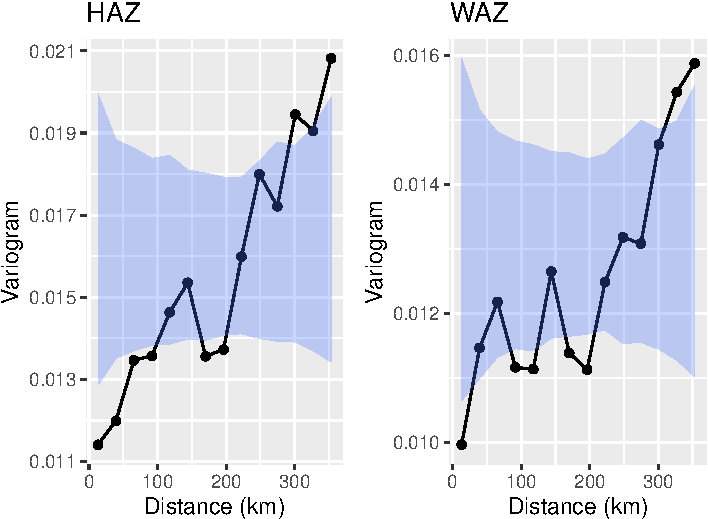
\includegraphics[keepaspectratio]{05_case-studies_files/figure-pdf/fig-maln-vari-1.pdf}}

}

\caption{\label{fig-maln-vari}Empirical variograms for HAZ and WAZ based
on the estimated random effects from Equation~\ref{eq-model-haz-waz}.}

\end{figure}%

Figure~\ref{fig-maln-vari} shows the variogram for both HAZ and WAZ. In
both cases, we observe that is residual spatial correlation in the data
that is not explained by either age or the wealth index. We next extend
the model in Equation~\ref{eq-model-haz-waz} to address this issue.

For our geostatistical analysis of HAZ and WAZ, we consider the
following model:

\[
Y_{ij} = \beta_0 + \beta_1 a_{ij} + \beta_2 \max\{a_{ij} - c, 0\} + \beta_3 w_i + S(x_i) + U_{ij},
\]

where \(S(x)\) is a zero-mean, stationary, and isotropic Gaussian
process with variance \(\sigma^2\) and an exponential correlation
function with scale parameter \(\phi\). In this geostatistical
extension, we replace the cluster-level random effect \(Z_i\) from
Equation~\ref{eq-model-haz-waz} with the spatial process \(S(x_i)\). The
random effect \(Z_i\) was previously used in the Binomial mixed model to
account for unexplained variation between clusters. It is also possible
to include both \(S(x_i)\) and \(Z_i\) in the model, so that the total
unexplained variation between clusters is decomposed into a spatially
structured component, \(S(x_i)\), and an unstructured component,
\(Z_i\). However, this approach is not recommended in the initial model
specification, as it may lead to identifiability issues. It can be
considered later in the analysis if justified by model diagnostics.

\begin{Shaded}
\begin{Highlighting}[]
\CommentTok{\# Remove missing data from the WAZ outcome}
\NormalTok{malnutrition }\OtherTok{\textless{}{-}}\NormalTok{ malnutrition[}\FunctionTok{complete.cases}\NormalTok{(malnutrition[,}\StringTok{"WAZ"}\NormalTok{]),]}

\CommentTok{\# Converting the data{-}frame into an sf object}
\NormalTok{malnutrition\_sf }\OtherTok{\textless{}{-}} \FunctionTok{st\_as\_sf}\NormalTok{(malnutrition, }\AttributeTok{coords =} \FunctionTok{c}\NormalTok{(}\StringTok{"lng"}\NormalTok{, }\StringTok{"lat"}\NormalTok{), }\AttributeTok{crs =} \DecValTok{4326}\NormalTok{)}
\NormalTok{malnutrition\_sf }\OtherTok{\textless{}{-}} \FunctionTok{st\_transform}\NormalTok{(malnutrition\_sf, }\AttributeTok{crs =} \FunctionTok{propose\_utm}\NormalTok{(malnutrition\_sf))}

\CommentTok{\# Maximum likelihood estimation for the HAZ and WAZ outcomes}
\NormalTok{haz\_fit }\OtherTok{\textless{}{-}} 
\FunctionTok{glgpm}\NormalTok{(HAZ }\SpecialCharTok{\textasciitilde{}}\NormalTok{ age }\SpecialCharTok{+} \FunctionTok{pmax}\NormalTok{(age }\SpecialCharTok{{-}} \DecValTok{1}\NormalTok{, }\DecValTok{0}\NormalTok{) }\SpecialCharTok{+}\NormalTok{ wealth }\SpecialCharTok{+} \FunctionTok{gp}\NormalTok{(),}
      \AttributeTok{data=}\NormalTok{malnutrition\_sf, }\AttributeTok{family =} \StringTok{"gaussian"}\NormalTok{)}

\NormalTok{waz\_fit }\OtherTok{\textless{}{-}} 
  \FunctionTok{glgpm}\NormalTok{(HAZ }\SpecialCharTok{\textasciitilde{}}\NormalTok{ age }\SpecialCharTok{+} \FunctionTok{pmax}\NormalTok{(age }\SpecialCharTok{{-}} \DecValTok{1}\NormalTok{, }\DecValTok{0}\NormalTok{) }\SpecialCharTok{+}\NormalTok{ wealth }\SpecialCharTok{+} \FunctionTok{gp}\NormalTok{(),}
        \AttributeTok{data=}\NormalTok{malnutrition\_sf, }\AttributeTok{family =} \StringTok{"gaussian"}\NormalTok{) }
\end{Highlighting}
\end{Shaded}

We then summarize the fit of models.

\begin{Shaded}
\begin{Highlighting}[]
\FunctionTok{summary}\NormalTok{(haz\_fit)}
\end{Highlighting}
\end{Shaded}

\begin{verbatim}
Call:
glgpm(formula = HAZ ~ age + pmax(age - 1, 0) + wealth + gp(), 
    data = malnutrition_sf, family = "gaussian")

Linear geostatistical model
Link: identity 
Inverse link function = x 
 
'Lower limit' and 'Upper limit' are the limits of the 95% confidence level intervals

Regression coefficients
                   Estimate Lower limit Upper limit     StdErr  z.value p.value
(Intercept)      -0.2158950  -0.4338747   0.0020848  0.1112162  -1.9412 0.05223
age              -1.3073560  -1.4135715  -1.2011404  0.0541926 -24.1243 < 2e-16
pmax(age - 1, 0)  1.2288215   1.1496224   1.3080207  0.0404085  30.4100 < 2e-16
wealth            0.3520544   0.3319696   0.3721393  0.0102476  34.3550 < 2e-16
                    
(Intercept)      .  
age              ***
pmax(age - 1, 0) ***
wealth           ***
---
Signif. codes:  0 '***' 0.001 '**' 0.01 '*' 0.05 '.' 0.1 ' ' 1

                        Estimate Lower limit Upper limit
Measuremment error var.   1.4371      1.4254      1.4489

Spatial Gaussian process
Matern covariance parameters (kappa=0.5)
                      Estimate Lower limit Upper limit
Spatial process var.  0.069453    0.061423      0.0785
Spatial corr. scale  36.529380   30.187727     44.2032
Variance of the nugget effect fixed at 0

Log-likelihood: -1859.246
AIC: 3732.491
\end{verbatim}

\begin{Shaded}
\begin{Highlighting}[]
\FunctionTok{summary}\NormalTok{(waz\_fit)}
\end{Highlighting}
\end{Shaded}

\begin{verbatim}
Call:
glgpm(formula = WAZ ~ age + pmax(age - 1, 0) + wealth + gp(), 
    data = malnutrition_sf, family = "gaussian")

Linear geostatistical model
Link: identity 
Inverse link function = x 
 
'Lower limit' and 'Upper limit' are the limits of the 95% confidence level intervals

Regression coefficients
                   Estimate Lower limit Upper limit     StdErr  z.value
(Intercept)      -0.4580088  -0.6499668  -0.2660509  0.0979395  -4.6764
age              -0.7295504  -0.8235412  -0.6355596  0.0479554 -15.2131
pmax(age - 1, 0)  0.7421647   0.6720850   0.8122443  0.0357556  20.7566
wealth            0.2254477   0.2076797   0.2432157  0.0090655  24.8689
                   p.value    
(Intercept)      2.919e-06 ***
age              < 2.2e-16 ***
pmax(age - 1, 0) < 2.2e-16 ***
wealth           < 2.2e-16 ***
---
Signif. codes:  0 '***' 0.001 '**' 0.01 '*' 0.05 '.' 0.1 ' ' 1

                        Estimate Lower limit Upper limit
Measuremment error var.   1.1253      1.1161      1.1346

Spatial Gaussian process
Matern covariance parameters (kappa=0.5)
                      Estimate Lower limit Upper limit
Spatial process var.  0.049912    0.043750      0.0569
Spatial corr. scale  35.836303   28.815346     44.5679
Variance of the nugget effect fixed at 0

Log-likelihood: -1530.593
AIC: 3075.187
\end{verbatim}

The spatial component of the models reveals a moderate degree of spatial
structure in the HAZ and WAZ outcomes. For HAZ, the estimated spatial
variance is approximately 0.069, while the individual-level radom
effect's variance is substantially larger at around 1.437. For WAZ, the
spatial variance is estimated at 0.050, compared to the variance of the
individual-level radom effect's variance of 1.125. In both models, as
already observed when fitting Binomial mixed models, this indicates that
the majority of the residual variation is due to individual-level noise
or unstructured heterogeneity rather than spatially structured effects.
The relative contribution of the spatial process to the total
unexplained variation is therefore relatively small. Nevertheless,
geostatistical analysis remains valuable also in this context. Even when
spatial effects explain only a modest proportion of the variation, the
model still enables spatial prediction of the average spatial pattern
for the outcome of interest across the study area. This is useful for
identifying areas where child malnutrition is systematically higher or
lower, guiding targeted interventions and informing resource allocation.
We explore these implications further in the next section on
geostatistical prediction for HAZ and WAZ.

\subsection{Prediction and assessment of model
calibration}\label{prediction-and-assessment-of-model-calibration}

Stunting and underweight are standard indicators used to assess child
malnutrition. A child is defined as \textit{stunted} if their
height-for-age \(z\)-score (HAZ) is below \(-2\) standard deviations
from the median of the WHO Child Growth Standards, i.e., HAZ \textless{}
-2. Similarly, a child is considered \textit{underweight} if their
weight-for-age \(z\)-score (WAZ) falls below \(-2\), i.e., WAZ
\textless{} -2 (United Nations Statistics Division, World Health
Organization, and UNICEF 2025). These thresholds are based on the World
Health Organization (WHO) growth reference standards, which provide a
normative basis for assessing nutritional status in children under five
years of age (Organization 2024).

We now define the predictive targets for stunting and underweight
prevalence in terms of the adopted geostatistical model. Both indicators
correspond to the probability that a child's z-score falls below \(-2\),
that is, \(Y(x) < -2\), where \(Y(x)\) denotes either the HAZ or WAZ
score at location \(x\). Under the model specification, the prevalence
is therefore defined as

\begin{equation}\phantomsection\label{eq-prev-maln}{
T(x) = P\left\{ Y(x) < -2 \,\middle|\, S(x) \right\} = \Phi\left( -\frac{\mu + S(x) + 2}{\omega} \right),
}\end{equation}

where \(\Phi(\cdot)\) is the cumulative distribution function of the
standard normal distribution, \(\mu\) is the linear predictor including
the effects of covariates at individual- and cluster-level (as defined
by the coefficients \(\beta_1\) to \(\beta_3\) of
Equation~\ref{eq-model-haz-waz}) as well as the intercept, and
\(\omega^2\) is the variance of the individual-level residual term. In
Equation~\ref{eq-prev-maln}, we condition on \(S(x)\) because this
allows us to define both stunting an underweight prevalence as a
spatially varying predictive target.

To implement this in \texttt{RiskMap}, we begin by generating a
predictive grid over the study region. In this case, we use a regular
grid with 10 km by 10 km resolution. We then draw predictive samples of
the spatial effect \(S(x)\) at each grid location, conditional on the
observed data. For the \texttt{age} variable, we fix it at 2 months for
HAZ and 1 month for WAZ, respectively. The \texttt{wealth} variable is
set to its lowest value of 1. These choices are made to visualize the
predictive target for the subgroup of children most at risk of stunting
and underweight, as identified through exploratory analysis and the
estimated regression coefficients. The code below illustrates this
procedure.

\begin{Shaded}
\begin{Highlighting}[]
\CommentTok{\# Boundaries of Ghana}
\FunctionTok{library}\NormalTok{(rgeoboundaries)}
\NormalTok{ghana }\OtherTok{\textless{}{-}} \FunctionTok{geoboundaries}\NormalTok{(}\AttributeTok{country =} \StringTok{"Ghana"}\NormalTok{, }\AttributeTok{adm\_lvl =} \StringTok{"adm0"}\NormalTok{)}
\NormalTok{ghana }\OtherTok{\textless{}{-}} \FunctionTok{st\_transform}\NormalTok{(ghana, }\FunctionTok{st\_crs}\NormalTok{(malnutrition\_sf))}

\NormalTok{ghana\_grid }\OtherTok{\textless{}{-}} \FunctionTok{create\_grid}\NormalTok{(ghana, }\AttributeTok{spat\_res =} \DecValTok{10}\NormalTok{)}

\NormalTok{n\_pred }\OtherTok{\textless{}{-}} \FunctionTok{nrow}\NormalTok{(}\FunctionTok{st\_coordinates}\NormalTok{(ghana\_grid))}

\CommentTok{\# Prediction of S(x) and covariates effects over the grid for}

\CommentTok{\# HAZ}
\NormalTok{haz\_pred\_grid }\OtherTok{\textless{}{-}} \FunctionTok{pred\_over\_grid}\NormalTok{(haz\_fit,}
                                \AttributeTok{grid\_pred =}\NormalTok{ ghana\_grid,}
                                \AttributeTok{predictors =} \FunctionTok{data.frame}\NormalTok{(}
                                  \CommentTok{\# Setting age to 2 months}
                                  \AttributeTok{age =} \FunctionTok{rep}\NormalTok{(}\DecValTok{2}\NormalTok{, n\_pred),}
                                  \CommentTok{\# Setting wealth to 1 (least wealthy)}
                                  \AttributeTok{wealth =} \FunctionTok{rep}\NormalTok{(}\DecValTok{1}\NormalTok{, n\_pred)}
\NormalTok{                                ))}
\CommentTok{\# WAZ}
\NormalTok{waz\_pred\_grid }\OtherTok{\textless{}{-}} \FunctionTok{pred\_over\_grid}\NormalTok{(waz\_fit,}
                                \AttributeTok{grid\_pred =}\NormalTok{ ghana\_grid,}
                                \AttributeTok{predictors =} \FunctionTok{data.frame}\NormalTok{(}
                                  \CommentTok{\# Setting age to 1 month}
                                  \AttributeTok{age =} \FunctionTok{rep}\NormalTok{(}\DecValTok{1}\NormalTok{, n\_pred),}
                                  \CommentTok{\# Setting wealth to 1 (least wealthy)}
                                  \AttributeTok{wealth =} \FunctionTok{rep}\NormalTok{(}\DecValTok{1}\NormalTok{, n\_pred)}
\NormalTok{                                ))}
\end{Highlighting}
\end{Shaded}

We then use the \texttt{pred\_target\_grid} function to generate
predictive summaries of stunting and underweight prevalence, as defined
in Equation~\ref{eq-prev-maln}. To quantify uncertainty in the
predictions, we report the coefficient of variation, which provides a
standardized measure of relative uncertainty across the prediction grid.

\begin{Shaded}
\begin{Highlighting}[]
\CommentTok{\# Prediction of stunting prevalence}
\NormalTok{sd\_ind\_haz }\OtherTok{\textless{}{-}} \FunctionTok{sqrt}\NormalTok{(}\FunctionTok{coef}\NormalTok{(haz\_fit)}\SpecialCharTok{$}\NormalTok{sigma2\_me)}
\NormalTok{stunting\_prev }\OtherTok{\textless{}{-}}
\FunctionTok{pred\_target\_grid}\NormalTok{(haz\_pred\_grid,}
                 \AttributeTok{f\_target =} \FunctionTok{list}\NormalTok{(}\AttributeTok{prev =} \ControlFlowTok{function}\NormalTok{(x) }\FunctionTok{pnorm}\NormalTok{((}\SpecialCharTok{{-}}\DecValTok{2}\SpecialCharTok{{-}}\NormalTok{x)}\SpecialCharTok{/}\NormalTok{sd\_ind\_haz)),}
                 \AttributeTok{pd\_summary =} \FunctionTok{list}\NormalTok{(}\AttributeTok{mean =}\NormalTok{ mean,}
                                       \AttributeTok{cv =} \ControlFlowTok{function}\NormalTok{(x) }\FunctionTok{sd}\NormalTok{(x)}\SpecialCharTok{/}\FunctionTok{mean}\NormalTok{(x)))}

\CommentTok{\# Prediction of underweight prevalence}
\NormalTok{sd\_ind\_waz }\OtherTok{\textless{}{-}} \FunctionTok{sqrt}\NormalTok{(}\FunctionTok{coef}\NormalTok{(waz\_fit)}\SpecialCharTok{$}\NormalTok{sigma2\_me)}
\NormalTok{underw\_prev }\OtherTok{\textless{}{-}}
  \FunctionTok{pred\_target\_grid}\NormalTok{(waz\_pred\_grid,}
                   \AttributeTok{f\_target =} \FunctionTok{list}\NormalTok{(}\AttributeTok{prev =} \ControlFlowTok{function}\NormalTok{(x) }\FunctionTok{pnorm}\NormalTok{((}\SpecialCharTok{{-}}\DecValTok{2}\SpecialCharTok{{-}}\NormalTok{x)}\SpecialCharTok{/}\NormalTok{sd\_ind\_waz)),}
                   \AttributeTok{pd\_summary =} \FunctionTok{list}\NormalTok{(}\AttributeTok{mean =}\NormalTok{ mean,}
                                     \AttributeTok{cv =} \ControlFlowTok{function}\NormalTok{(x) }\FunctionTok{sd}\NormalTok{(x)}\SpecialCharTok{/}\FunctionTok{mean}\NormalTok{(x)))}
\end{Highlighting}
\end{Shaded}

Finally, we visualize the results in the map shown in
Figure~\ref{fig-maln-pred}. The maps reveal a clear hotspot for both
stunting and underweight, with predicted prevalence values reaching
approximately \(45\%\) and \(24\%\), respectively. Notably, this same
region also exhibits lower predictive uncertaint, measured by the
coefficient of variation, compared to other areas in Ghana.

\begin{Shaded}
\begin{Highlighting}[]
\CommentTok{\# Set up a 2x2 layout}
\FunctionTok{layout}\NormalTok{(}\FunctionTok{matrix}\NormalTok{(}\DecValTok{1}\SpecialCharTok{:}\DecValTok{4}\NormalTok{, }\AttributeTok{nrow =} \DecValTok{2}\NormalTok{, }\AttributeTok{byrow =} \ConstantTok{TRUE}\NormalTok{))}
\FunctionTok{par}\NormalTok{(}\AttributeTok{mar =} \FunctionTok{c}\NormalTok{(}\DecValTok{4}\NormalTok{, }\DecValTok{4}\NormalTok{, }\DecValTok{4}\NormalTok{, }\DecValTok{5}\NormalTok{))  }\CommentTok{\# Adjust margins}

\CommentTok{\# Top row: stunting}
\FunctionTok{plot}\NormalTok{(stunting\_prev, }\AttributeTok{which\_target =} \StringTok{"prev"}\NormalTok{, }\AttributeTok{which\_summary =} \StringTok{"mean"}\NormalTok{,}
     \AttributeTok{main =} \StringTok{"Stunting: Predictive Mean"}\NormalTok{)}
\FunctionTok{plot}\NormalTok{(stunting\_prev, }\AttributeTok{which\_target =} \StringTok{"prev"}\NormalTok{, }\AttributeTok{which\_summary =} \StringTok{"cv"}\NormalTok{,}
     \AttributeTok{main =} \StringTok{"Stunting: Coefficient of Variation"}\NormalTok{)}

\CommentTok{\# Bottom row: underweight}
\FunctionTok{plot}\NormalTok{(underw\_prev, }\AttributeTok{which\_target =} \StringTok{"prev"}\NormalTok{, }\AttributeTok{which\_summary =} \StringTok{"mean"}\NormalTok{,}
     \AttributeTok{main =} \StringTok{"Underweight: Predictive Mean"}\NormalTok{)}
\FunctionTok{plot}\NormalTok{(underw\_prev, }\AttributeTok{which\_target =} \StringTok{"prev"}\NormalTok{, }\AttributeTok{which\_summary =} \StringTok{"cv"}\NormalTok{,}
     \AttributeTok{main =} \StringTok{"Underweight: Coefficient of Variation"}\NormalTok{)}
\end{Highlighting}
\end{Shaded}

\begin{figure}[H]

\centering{

\pandocbounded{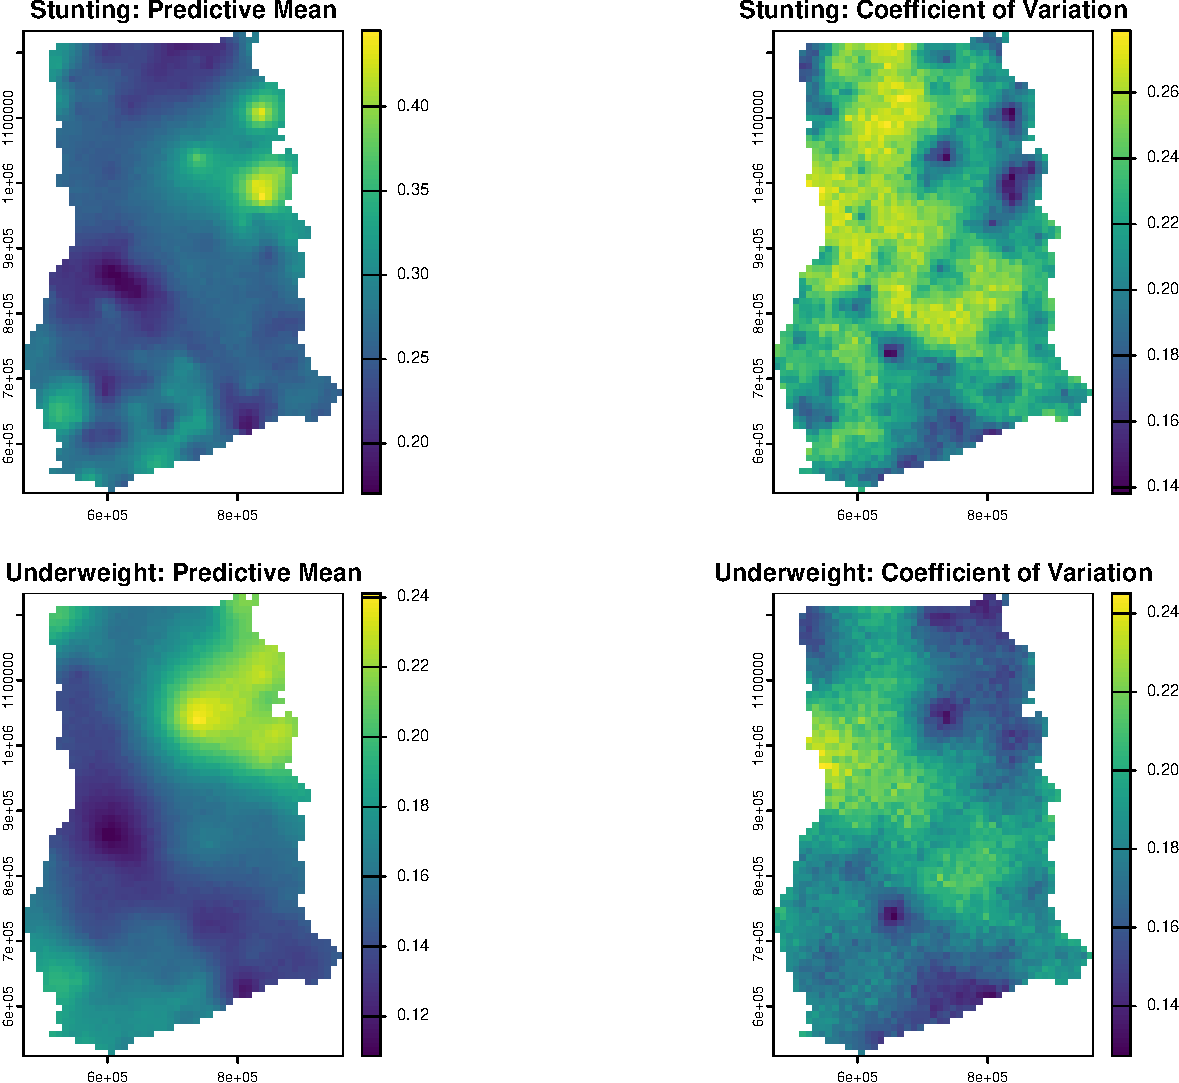
\includegraphics[keepaspectratio]{05_case-studies_files/figure-pdf/fig-maln-pred-1.pdf}}

}

\caption{\label{fig-maln-pred}Predictive mean and coefficient of
variation for stunting and underweight prevalence estimates. The top row
shows predictions for stunting, while the bottom row corresponds to
underweight. For each indicator, the left panel shows the predictive
mean and the right panel the coefficient of variation.}

\end{figure}%

To assess the predictive performance and calibration of our
geostatistical models for HAZ and WAZ, we perform a cross-validation
exercise using the \texttt{assess\_pp} function. Cross-validation is
conducted by repeatedly splitting the data into training and testing
sets, ensuring that prediction locations are at least 5 km away from the
nearest training point. Specifically, we set \texttt{n\_size\ =\ 100}
prediction locations for the test set, impose a minimum distance
constraint of 5 km (\texttt{min\_dist\ =\ 5}), and repeat the process
over 10 test sets randomly drawn under those conditions
(\texttt{iter\ =\ 10}) using \texttt{method="regularized"} as the
sampling method.

\begin{Shaded}
\begin{Highlighting}[]
\CommentTok{\# HAZ}
\NormalTok{assess\_haz }\OtherTok{\textless{}{-}}
\FunctionTok{assess\_pp}\NormalTok{(}\FunctionTok{list}\NormalTok{(}\AttributeTok{HAZ =}\NormalTok{ haz\_fit),}
          \AttributeTok{n\_size =} \DecValTok{100}\NormalTok{,}
          \AttributeTok{min\_dist =} \DecValTok{5}\NormalTok{,}
          \AttributeTok{iter =} \DecValTok{10}\NormalTok{,}
          \AttributeTok{method =} \StringTok{"regularized"}\NormalTok{)}

\CommentTok{\# WAZ}
\NormalTok{assess\_waz }\OtherTok{\textless{}{-}}
  \FunctionTok{assess\_pp}\NormalTok{(}\FunctionTok{list}\NormalTok{(}\AttributeTok{WAZ =}\NormalTok{ waz\_fit),}
            \AttributeTok{n\_size =} \DecValTok{100}\NormalTok{,}
            \AttributeTok{min\_dist =} \DecValTok{5}\NormalTok{,}
            \AttributeTok{iter =} \DecValTok{10}\NormalTok{,}
            \AttributeTok{method =} \StringTok{"regularized"}\NormalTok{)}
\end{Highlighting}
\end{Shaded}

We note that for a Gaussian linear geostatistical model, the
\texttt{assess\_pp} function does not compute the average non-randomized
probability integral transform (AnPIT, introduced in
Section~\ref{sec-anpit}), as this measure is specifically designed for
count outcomes. Instead, it employs the standard probability integral
transform (PIT), defined as \(\text{PIT}(y) = F_{M}(y)\), where
\(F_{M}(y)\) is the cumulative distribution function of the predictive
distribution evaluated at the observed value \(y\). The PIT transforms
the observed outcomes in the test set such that, if the model is
well-calibrated, these transformed values should follow a uniform
distribution. Deviations from uniformity indicate potential issues with
calibration and predictive accuracy.

Figure~\ref{fig-maln-pit} shows the results of the cross-validation
exercise visualized through PIT curves for HAZ and WAZ. Similarly to the
way we have interpreted the AnPIT curves, the PIT curves indicate good
calibration when they lie close to the identity line, meaning the
predictive distributions accurately reflect the observed variability in
the test sets. The results shown in Figure~\ref{fig-maln-pit}
demonstrate that, for all ten test sets and for both HAZ and WAZ, the
PIT curves closely align with the identity line, confirming that the
models are well-calibrated and provide reliable uncertainty
quantification.

\begin{Shaded}
\begin{Highlighting}[]
\CommentTok{\# Generate PIT plots}
\NormalTok{p\_haz }\OtherTok{\textless{}{-}} \FunctionTok{plot\_AnPIT}\NormalTok{(assess\_haz, }\AttributeTok{mode =} \StringTok{"all"}\NormalTok{)}
\NormalTok{p\_waz }\OtherTok{\textless{}{-}} \FunctionTok{plot\_AnPIT}\NormalTok{(assess\_waz, }\AttributeTok{mode =} \StringTok{"all"}\NormalTok{)}

\CommentTok{\# Arrange side{-}by{-}side}
\FunctionTok{library}\NormalTok{(gridExtra)}
\FunctionTok{grid.arrange}\NormalTok{(p\_haz, p\_waz, }\AttributeTok{ncol =} \DecValTok{2}\NormalTok{)}
\end{Highlighting}
\end{Shaded}

\begin{figure}[H]

\centering{

\pandocbounded{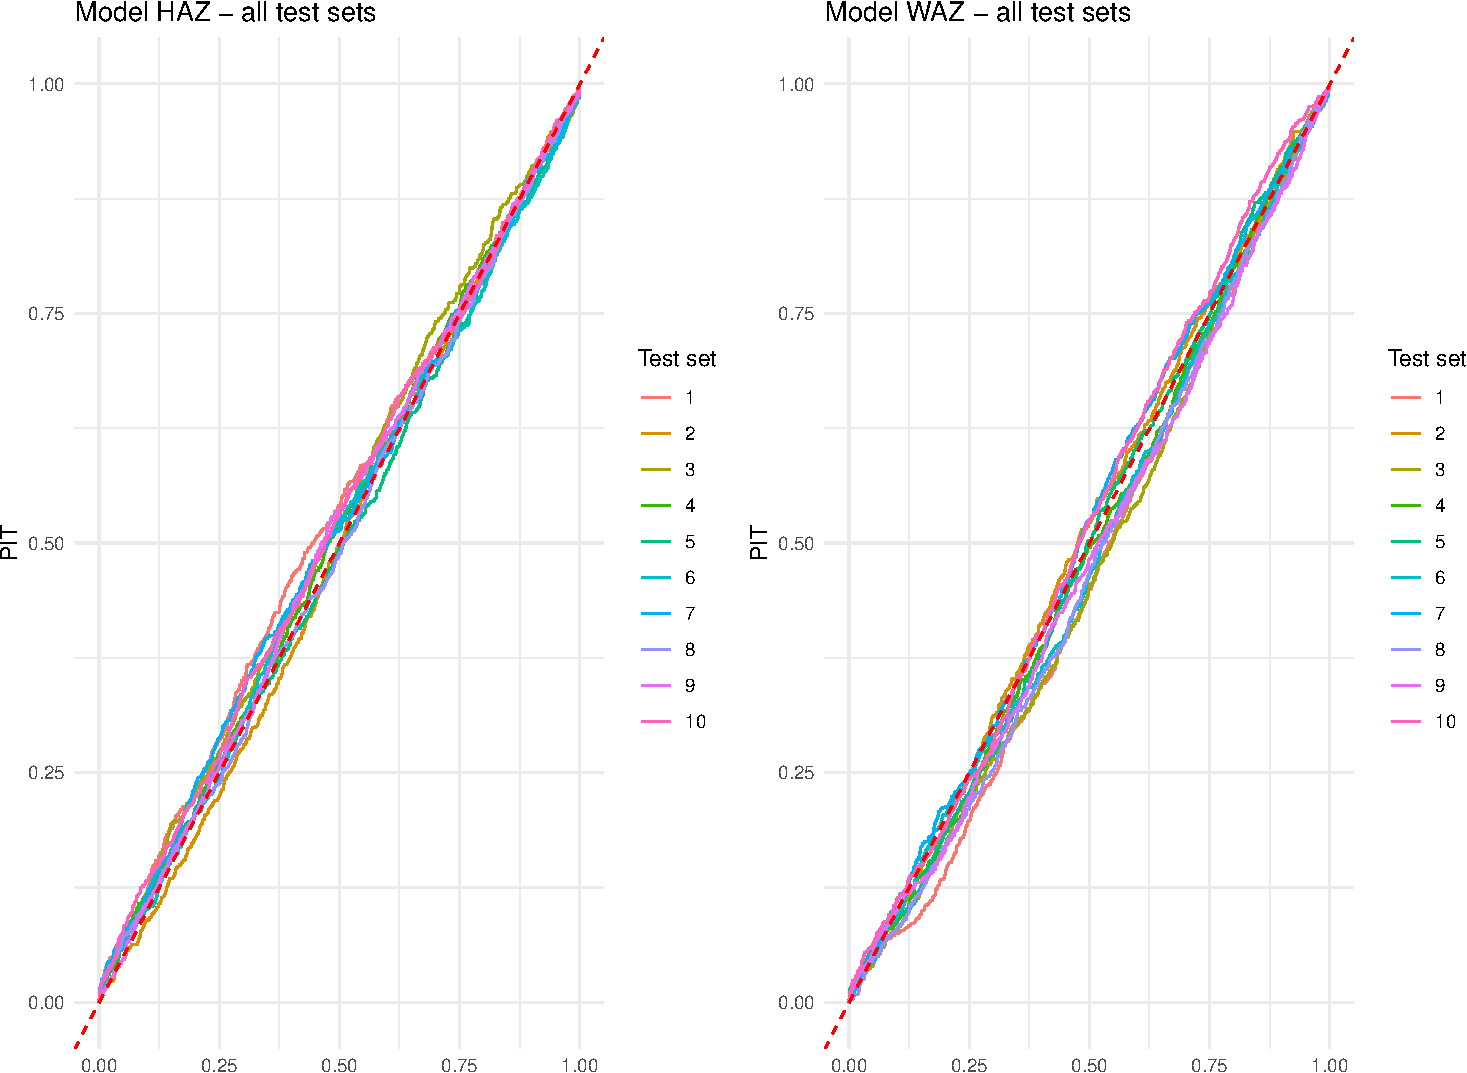
\includegraphics[keepaspectratio]{05_case-studies_files/figure-pdf/fig-maln-pit-1.pdf}}

}

\caption{\label{fig-maln-pit}Assessment of the models calibration. The
left panel shows the probability integral transform (PIT) curve for HAZ,
and the right panel for WAZ. In both panels, the red dahsed line
corresponds to the identity line.}

\end{figure}%

\subsection{Summary and conclusions}\label{summary-and-conclusions}

This case study demonstrated the utility of geostatistical modeling for
mapping child malnutrition in Ghana using continuous anthropometric
measurements, namely HAZ and WAZ Z-scores. By modeling these outcomes
directly, we were able to define stunting and underweight prevalence as
predictive probabilities based on threshold exceedance (e.g., HAZ
\textless{} -2), rather than by dichotomizing the data prior to
analysis. This approach allowed us to retain the full information
content of the measurements and to produce spatially resolved
predictions of prevalence along with associated uncertainty estimates.
Readers interested in a more in-depth treatment of this modeling
strategy are referred to Kyomuhangi et al. (2021), which discusses the
loss of information and degradation in predictive performance that can
result from dichotomizing continuous outcomes in geostatistical
settings.

More broadly, this case study illustrated how geostatistical models can
be used to analyze individual-level outcomes while accounting for both
child-level and household-level covariates. Aggregation of data across
individuals, such as using average HAZ or WAZ scores per location, is
not required and can in fact introduce several complications. In
particular, the number of children per cluster varies, which implies
that an analysis based on cluster-level averages would require a
heteroscedastic specification for the residual term to appropriately
reflect varying precision across locations. Ignoring this could lead to
unreliable predictive inferences.

In conclusion, this analysis showed that neither dichotomization nor
aggregation is necessary in geostaistical analysis. Instead,
geostatistical models should be fitted to individual-level continuous
outcomes, and suitable predictive targets and summaries of uncertainty
can then be derived from the fitted model.

\section{Mapping malaria in Malawi}\label{mapping-malaria-in-malawi}

In this section, we demonstrate how to conduct a geostatistical analysis
using Malaria Indicator Survey (MIS) data accessed through the
\texttt{malariaAtlas} R package (Lucas et al. 2020). This package
provides streamlined access to a curated repository of georeferenced
malaria data, including prevalence surveys and associated metadata,
making it a valuable resource for spatial epidemiological studies. The
primary aim here is to illustrate how relevant environmental covariates
can be obtained via Google Earth Engine and incorporated into a
geostatistical model for prevalence mapping. Although the analysis is
not guided by a specific research question, its value lies in showcasing
the full workflow and technical aspects introduced in previous chapters,
including data preparation, covariate extraction, exploratory analysis,
model fitting, and spatial prediction of disease prevalence.

\subsection{Downloading prevalence and raster
data}\label{downloading-prevalence-and-raster-data}

This section illustrates how to access and visualize Malaria Indicator
Survey data using the \texttt{malariaAtlas} R package, focusing on
\emph{Plasmodium falciparum} prevalence in Malawi for the year 2006. We
walk through the steps to extract survey data, obtain country
boundaries, and produce a basic map of raw prevalence data.

We begin by loading the necessary packages and initializing the Earth
Engine API via the \texttt{rgee} package.

\begin{Shaded}
\begin{Highlighting}[]
\CommentTok{\# Load libraries}
\FunctionTok{library}\NormalTok{(malariaAtlas)}
\FunctionTok{library}\NormalTok{(dplyr)}
\FunctionTok{library}\NormalTok{(tidyr)}
\FunctionTok{library}\NormalTok{(sf)}
\FunctionTok{library}\NormalTok{(rgee)}
\FunctionTok{library}\NormalTok{(terra)}
\FunctionTok{library}\NormalTok{(rgeoboundaries)}
\FunctionTok{library}\NormalTok{(grid)}

\CommentTok{\# Initialize Earth Engine}
\FunctionTok{ee\_Initialize}\NormalTok{()}
\end{Highlighting}
\end{Shaded}

We then use \texttt{rgeoboundaries} to obtain Malawi's administrative
boundary and extract P. falciparum prevalence survey data from the
\texttt{malariaAtlas} package for surveys conducted in or overlapping
the year 2006.

\begin{Shaded}
\begin{Highlighting}[]
\CommentTok{\# Get Malawi boundary}
\NormalTok{mlw\_admin0\_sf }\OtherTok{\textless{}{-}} \FunctionTok{geoboundaries}\NormalTok{(}\AttributeTok{country =} \StringTok{"Malawi"}\NormalTok{, }\AttributeTok{adm\_lvl =} \StringTok{"adm0"}\NormalTok{)}
\NormalTok{mlw\_admin0\_ee }\OtherTok{\textless{}{-}} \FunctionTok{sf\_as\_ee}\NormalTok{(mlw\_admin0\_sf)}

\CommentTok{\# Download PfPR survey data}
\NormalTok{mlw\_pfpr }\OtherTok{\textless{}{-}} \FunctionTok{getPR}\NormalTok{(}\AttributeTok{country =} \StringTok{"Malawi"}\NormalTok{, }\AttributeTok{species =} \StringTok{"Pf"}\NormalTok{) }\SpecialCharTok{\%\textgreater{}\%}
  \FunctionTok{filter}\NormalTok{(year\_start }\SpecialCharTok{\textless{}=} \DecValTok{2006} \SpecialCharTok{\&}\NormalTok{ year\_end }\SpecialCharTok{\textgreater{}=} \DecValTok{2006}\NormalTok{) }\SpecialCharTok{\%\textgreater{}\%}
  \FunctionTok{filter}\NormalTok{(}\SpecialCharTok{!}\FunctionTok{is.na}\NormalTok{(longitude) }\SpecialCharTok{\&} \SpecialCharTok{!}\FunctionTok{is.na}\NormalTok{(latitude))}

\CommentTok{\# Convert to sf object}
\NormalTok{mlw\_sf }\OtherTok{\textless{}{-}} \FunctionTok{st\_as\_sf}\NormalTok{(mlw\_pfpr, }\AttributeTok{coords =} \FunctionTok{c}\NormalTok{(}\StringTok{"longitude"}\NormalTok{, }\StringTok{"latitude"}\NormalTok{), }\AttributeTok{crs =} \DecValTok{4326}\NormalTok{)}

\CommentTok{\# Convert to UTM }
\NormalTok{mlw\_crs }\OtherTok{\textless{}{-}} \FunctionTok{propose\_utm}\NormalTok{(mlw\_sf)}
\NormalTok{mlw\_sf }\OtherTok{\textless{}{-}} \FunctionTok{st\_transform}\NormalTok{(mlw\_sf, }\AttributeTok{crs =}\NormalTok{ mlw\_crs)}

\CommentTok{\# Remove columns with all NAs}
\NormalTok{mlw\_sf }\OtherTok{\textless{}{-}}\NormalTok{ mlw\_sf[, }\FunctionTok{colSums}\NormalTok{(}\SpecialCharTok{!}\FunctionTok{is.na}\NormalTok{(mlw\_sf)) }\SpecialCharTok{\textgreater{}} \DecValTok{0}\NormalTok{]}
\end{Highlighting}
\end{Shaded}

The following map displays the raw prevalence data at each survey
location. The size and color of each point reflect the estimated malaria
prevalence (pr) at that location.

\begin{Shaded}
\begin{Highlighting}[]
\CommentTok{\# Compute prevalence}
\CommentTok{\# Compute observed prevalence}
\NormalTok{mlw\_sf}\SpecialCharTok{$}\NormalTok{pr }\OtherTok{\textless{}{-}}\NormalTok{ mlw\_sf}\SpecialCharTok{$}\NormalTok{positive }\SpecialCharTok{/}\NormalTok{ mlw\_sf}\SpecialCharTok{$}\NormalTok{examined}

\CommentTok{\# Plot raw PfPR data with uniform point size and no axis labels}
\FunctionTok{ggplot}\NormalTok{() }\SpecialCharTok{+}
  \FunctionTok{geom\_sf}\NormalTok{(}\AttributeTok{data =}\NormalTok{ mlw\_admin0\_sf, }\AttributeTok{fill =} \StringTok{"white"}\NormalTok{, }\AttributeTok{color =} \StringTok{"black"}\NormalTok{) }\SpecialCharTok{+}
  \FunctionTok{geom\_sf}\NormalTok{(}\AttributeTok{data =}\NormalTok{ mlw\_sf, }\FunctionTok{aes}\NormalTok{(}\AttributeTok{color =}\NormalTok{ pr), }\AttributeTok{size =} \DecValTok{1}\NormalTok{, }\AttributeTok{alpha =} \FloatTok{0.8}\NormalTok{) }\SpecialCharTok{+}
  \FunctionTok{scale\_color\_viridis\_c}\NormalTok{(}\AttributeTok{name =} \StringTok{"PfPR"}\NormalTok{) }\SpecialCharTok{+}
  \FunctionTok{theme\_minimal}\NormalTok{() }\SpecialCharTok{+}
  \FunctionTok{ggtitle}\NormalTok{(}\StringTok{"Malaria Prevalence in Malawi (2006)"}\NormalTok{) }\SpecialCharTok{+}
  \FunctionTok{theme}\NormalTok{(}
    \AttributeTok{legend.position =} \StringTok{"right"}\NormalTok{,}
    \AttributeTok{axis.title =} \FunctionTok{element\_blank}\NormalTok{(),}
    \AttributeTok{axis.text =} \FunctionTok{element\_blank}\NormalTok{(),}
    \AttributeTok{axis.ticks =} \FunctionTok{element\_blank}\NormalTok{()}
\NormalTok{  )}
\end{Highlighting}
\end{Shaded}

\begin{figure}[H]

\centering{

\pandocbounded{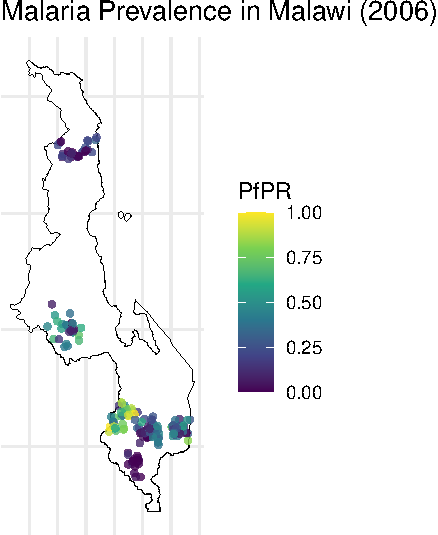
\includegraphics[keepaspectratio]{05_case-studies_files/figure-pdf/fig-malawi-raw-map-1.pdf}}

}

\caption{\label{fig-malawi-raw-map}Raw PfPR survey data for Malawi in
2006. Each point represents a georeferenced survey location, with color
and size indicating estimated prevalence.}

\end{figure}%

In the next step we retrieve a suite of environmental covariates that
are mechanistically linked to malaria transmission and therefore
commonly included in spatial risk-mapping studies. All layers are
clipped to the Malawi national boundary and combined into a single
multi-band image ready for extraction at the survey points.

These covariates are summarised in Table~Table~\ref{tbl-covariates},
which also explains their epidemiological relevance in the context of
malaria transmission.

\begin{longtable}[]{@{}
  >{\raggedright\arraybackslash}p{(\linewidth - 6\tabcolsep) * \real{0.2500}}
  >{\raggedright\arraybackslash}p{(\linewidth - 6\tabcolsep) * \real{0.2500}}
  >{\raggedright\arraybackslash}p{(\linewidth - 6\tabcolsep) * \real{0.2500}}
  >{\raggedright\arraybackslash}p{(\linewidth - 6\tabcolsep) * \real{0.2500}}@{}}
\caption{Environmental covariates extracted from Google Earth Engine and
their relevance for malaria risk
modelling.}\label{tbl-covariates}\tabularnewline
\toprule\noalign{}
\begin{minipage}[b]{\linewidth}\raggedright
Covariate
\end{minipage} & \begin{minipage}[b]{\linewidth}\raggedright
Source
\end{minipage} & \begin{minipage}[b]{\linewidth}\raggedright
Processing
\end{minipage} & \begin{minipage}[b]{\linewidth}\raggedright
Relevance
\end{minipage} \\
\midrule\noalign{}
\endfirsthead
\toprule\noalign{}
\begin{minipage}[b]{\linewidth}\raggedright
Covariate
\end{minipage} & \begin{minipage}[b]{\linewidth}\raggedright
Source
\end{minipage} & \begin{minipage}[b]{\linewidth}\raggedright
Processing
\end{minipage} & \begin{minipage}[b]{\linewidth}\raggedright
Relevance
\end{minipage} \\
\midrule\noalign{}
\endhead
\bottomrule\noalign{}
\endlastfoot
Precipitation & CHIRPS Daily & Annual mean (mm · day⁻¹) & Determines
suitability of breeding sites for \emph{Anopheles} mosquitoes. \\
Land-surface temperature & MODIS MOD11A2 & Kelvin converted to °C;
annual mean & Affects mosquito survival and parasite development
rates. \\
NDVI & MODIS MOD13A2 & Scaled to 0--1; annual mean & Proxy for habitat
moisture and vegetation cover. \\
Elevation & SRTM DEM & 90 m; clipped to country boundary & Integrates
climatic variation; highlands tend to have lower transmission. \\
Relative humidity & ERA5-Land & Derived from temperature and dew-point;
annual mean (\%) & High humidity increases mosquito survival. \\
Urbanicity (built-up areas) & MODIS MCD12Q1 & Binary indicator (class 13
= urban) & Urban areas generally have lower risk due to infrastructure
and fewer breeding sites. \\
\end{longtable}

We point out that in order to compute relative humidity, we first
extract hourly estimates of air temperature and dew-point temperature at
2 meters above ground level from the ERA5-Land reanalysis product. These
two quantities are then combined using a standard empirical formula
derived from the Clausius--Clapeyron relation: \[
\text{RH} = 100 \times \left( \frac{e^{\frac{17.625 \cdot T_d}{243.04 + T_d}}}{e^{\frac{17.625 \cdot T}{243.04 + T}}} \right)
\] where \(T_d\) is the dew-point temperature and \(T\) is the air
temperature, both in degrees Celsius. This yields the mean annual
relative humidity over the target region, expressed as a percentage.

Table~\ref{tbl-covariates} does not provide an exhaustive list of
covariates, and other factors such as soil moisture, land surface water,
nighttime temperature, or socio-economic indicators like night-time
light intensity and land surface emissivity, which may serve as proxies
for human activity, infrastructure, or economic development, could also
influence malaria risk. However, to maintain this illustrative analysis
simpler, we restrict our attention to a core set of covariates that
capture key climatic, ecological, and anthropogenic drivers.

In the code below, all layers are clipped to the boundary of Malawi and
combined into a single multi-band image, ready to be extracted at survey
point locations for subsequent modeling.

\begin{Shaded}
\begin{Highlighting}[]
\CommentTok{\# {-}{-}{-}{-}{-}{-}{-}{-}{-}{-}{-}{-}{-}{-}{-}{-}{-}{-}{-}{-}{-}{-}{-}{-}{-}{-}{-}{-}{-}{-}{-}}
\CommentTok{\# STEP 2: Covariates from Earth Engine}
\CommentTok{\# {-}{-}{-}{-}{-}{-}{-}{-}{-}{-}{-}{-}{-}{-}{-}{-}{-}{-}{-}{-}{-}{-}{-}{-}{-}{-}{-}{-}{-}{-}{-}}
\NormalTok{scale\_m }\OtherTok{\textless{}{-}} \DecValTok{1000}

\CommentTok{\# Precipitation}
\NormalTok{precip }\OtherTok{\textless{}{-}}\NormalTok{ ee}\SpecialCharTok{$}\FunctionTok{ImageCollection}\NormalTok{(}\StringTok{"UCSB{-}CHG/CHIRPS/DAILY"}\NormalTok{)}\SpecialCharTok{$}
  \FunctionTok{filterDate}\NormalTok{(}\StringTok{"2006{-}01{-}01"}\NormalTok{, }\StringTok{"2006{-}12{-}31"}\NormalTok{)}\SpecialCharTok{$}
  \FunctionTok{mean}\NormalTok{()}\SpecialCharTok{$}\FunctionTok{rename}\NormalTok{(}\StringTok{"precip"}\NormalTok{)}\SpecialCharTok{$}\FunctionTok{clip}\NormalTok{(mlw\_admin0\_ee)}\SpecialCharTok{$}\FunctionTok{toFloat}\NormalTok{()}

\CommentTok{\# Temperature}
\NormalTok{lst }\OtherTok{\textless{}{-}}\NormalTok{ ee}\SpecialCharTok{$}\FunctionTok{ImageCollection}\NormalTok{(}\StringTok{"MODIS/061/MOD11A2"}\NormalTok{)}\SpecialCharTok{$}
  \FunctionTok{filterDate}\NormalTok{(}\StringTok{"2006{-}01{-}01"}\NormalTok{, }\StringTok{"2006{-}12{-}31"}\NormalTok{)}\SpecialCharTok{$}
  \FunctionTok{select}\NormalTok{(}\StringTok{"LST\_Day\_1km"}\NormalTok{)}\SpecialCharTok{$}\FunctionTok{mean}\NormalTok{()}\SpecialCharTok{$}
  \FunctionTok{multiply}\NormalTok{(}\FloatTok{0.02}\NormalTok{)}\SpecialCharTok{$}\FunctionTok{subtract}\NormalTok{(}\FloatTok{273.15}\NormalTok{)}\SpecialCharTok{$}\FunctionTok{rename}\NormalTok{(}\StringTok{"lst\_c"}\NormalTok{)}\SpecialCharTok{$}
  \FunctionTok{clip}\NormalTok{(mlw\_admin0\_ee)}\SpecialCharTok{$}\FunctionTok{toFloat}\NormalTok{()}

\CommentTok{\# NDVI}
\NormalTok{ndvi }\OtherTok{\textless{}{-}}\NormalTok{ ee}\SpecialCharTok{$}\FunctionTok{ImageCollection}\NormalTok{(}\StringTok{"MODIS/061/MOD13A2"}\NormalTok{)}\SpecialCharTok{$}
  \FunctionTok{filterDate}\NormalTok{(}\StringTok{"2006{-}01{-}01"}\NormalTok{, }\StringTok{"2006{-}12{-}31"}\NormalTok{)}\SpecialCharTok{$}
  \FunctionTok{select}\NormalTok{(}\StringTok{"NDVI"}\NormalTok{)}\SpecialCharTok{$}\FunctionTok{mean}\NormalTok{()}\SpecialCharTok{$}
  \FunctionTok{multiply}\NormalTok{(}\FloatTok{0.0001}\NormalTok{)}\SpecialCharTok{$}\FunctionTok{rename}\NormalTok{(}\StringTok{"ndvi"}\NormalTok{)}\SpecialCharTok{$}
  \FunctionTok{clip}\NormalTok{(mlw\_admin0\_ee)}\SpecialCharTok{$}\FunctionTok{toFloat}\NormalTok{()}

\CommentTok{\# Elevation}
\NormalTok{elev }\OtherTok{\textless{}{-}}\NormalTok{ ee}\SpecialCharTok{$}\FunctionTok{Image}\NormalTok{(}\StringTok{"USGS/SRTMGL1\_003"}\NormalTok{)}\SpecialCharTok{$}
  \FunctionTok{rename}\NormalTok{(}\StringTok{"elev"}\NormalTok{)}\SpecialCharTok{$}\FunctionTok{clip}\NormalTok{(mlw\_admin0\_ee)}\SpecialCharTok{$}\FunctionTok{toFloat}\NormalTok{()}

\CommentTok{\# Humidity from ERA5 (computed from dewpoint and temperature)}
\NormalTok{era5 }\OtherTok{\textless{}{-}}\NormalTok{ ee}\SpecialCharTok{$}\FunctionTok{ImageCollection}\NormalTok{(}\StringTok{"ECMWF/ERA5\_LAND/HOURLY"}\NormalTok{)}\SpecialCharTok{$}
  \FunctionTok{filterDate}\NormalTok{(}\StringTok{"2006{-}01{-}01"}\NormalTok{, }\StringTok{"2006{-}12{-}31"}\NormalTok{)}\SpecialCharTok{$}
  \FunctionTok{select}\NormalTok{(}\FunctionTok{c}\NormalTok{(}\StringTok{"dewpoint\_temperature\_2m"}\NormalTok{, }\StringTok{"temperature\_2m"}\NormalTok{))}\SpecialCharTok{$}
  \FunctionTok{mean}\NormalTok{()}\SpecialCharTok{$}\FunctionTok{clip}\NormalTok{(mlw\_admin0\_ee)}

\NormalTok{td }\OtherTok{\textless{}{-}}\NormalTok{ era5}\SpecialCharTok{$}\FunctionTok{select}\NormalTok{(}\StringTok{"dewpoint\_temperature\_2m"}\NormalTok{)}\SpecialCharTok{$}\FunctionTok{subtract}\NormalTok{(}\FloatTok{273.15}\NormalTok{)}
\NormalTok{t }\OtherTok{\textless{}{-}}\NormalTok{ era5}\SpecialCharTok{$}\FunctionTok{select}\NormalTok{(}\StringTok{"temperature\_2m"}\NormalTok{)}\SpecialCharTok{$}\FunctionTok{subtract}\NormalTok{(}\FloatTok{273.15}\NormalTok{)}

\NormalTok{rh }\OtherTok{\textless{}{-}}\NormalTok{ td}\SpecialCharTok{$}\FunctionTok{expression}\NormalTok{(}
  \StringTok{"100 * (exp((17.625 * TD)/(243.04 + TD)) / exp((17.625 * T)/(243.04 + T)))"}\NormalTok{,}
  \FunctionTok{list}\NormalTok{(}\AttributeTok{TD =}\NormalTok{ td, }\AttributeTok{T =}\NormalTok{ t)}
\NormalTok{)}\SpecialCharTok{$}\FunctionTok{rename}\NormalTok{(}\StringTok{"humidity"}\NormalTok{)}\SpecialCharTok{$}\FunctionTok{toFloat}\NormalTok{()}

\CommentTok{\# Use MODIS Land Cover, version 061}
\NormalTok{urban\_raw }\OtherTok{\textless{}{-}}\NormalTok{ ee}\SpecialCharTok{$}\FunctionTok{ImageCollection}\NormalTok{(}\StringTok{"MODIS/061/MCD12Q1"}\NormalTok{)}\SpecialCharTok{$}
  \FunctionTok{filterDate}\NormalTok{(}\StringTok{"2006{-}01{-}01"}\NormalTok{, }\StringTok{"2006{-}12{-}31"}\NormalTok{)}\SpecialCharTok{$}
  \FunctionTok{first}\NormalTok{()}\SpecialCharTok{$}\FunctionTok{select}\NormalTok{(}\StringTok{"LC\_Type1"}\NormalTok{)}\SpecialCharTok{$}\FunctionTok{clip}\NormalTok{(mlw\_admin0\_ee)}

\CommentTok{\# Urban areas are class 13 in IGBP classification}
\NormalTok{built\_up }\OtherTok{\textless{}{-}}\NormalTok{ urban\_raw}\SpecialCharTok{$}\FunctionTok{eq}\NormalTok{(}\DecValTok{13}\NormalTok{)}\SpecialCharTok{$}\FunctionTok{rename}\NormalTok{(}\StringTok{"built\_up"}\NormalTok{)}\SpecialCharTok{$}\FunctionTok{toFloat}\NormalTok{()}



\CommentTok{\# Combine all covariates}
\NormalTok{covariates }\OtherTok{\textless{}{-}}\NormalTok{ precip}\SpecialCharTok{$}
  \FunctionTok{addBands}\NormalTok{(lst)}\SpecialCharTok{$}
  \FunctionTok{addBands}\NormalTok{(ndvi)}\SpecialCharTok{$}
  \FunctionTok{addBands}\NormalTok{(elev)}\SpecialCharTok{$}
  \FunctionTok{addBands}\NormalTok{(rh)}\SpecialCharTok{$}
  \FunctionTok{addBands}\NormalTok{(built\_up)}
\end{Highlighting}
\end{Shaded}

After defining the multi-band raster image \texttt{covariates} in Google
Earth Engine, we download it as a GeoTIFF file using the
\texttt{ee\_as\_rast()} function from the \texttt{rgee} package. The
file is saved temporarily and clipped to the bounding box of Malawi. We
then read the raster into R using the \texttt{terra}.

\begin{Shaded}
\begin{Highlighting}[]
\CommentTok{\# {-}{-}{-}{-}{-}{-}{-}{-}{-}{-}{-}{-}{-}{-}{-}{-}{-}{-}{-}{-}{-}{-}{-}{-}{-}{-}{-}{-}{-}{-}{-}}
\CommentTok{\# STEP 3: Download Earth Engine raster}
\CommentTok{\# {-}{-}{-}{-}{-}{-}{-}{-}{-}{-}{-}{-}{-}{-}{-}{-}{-}{-}{-}{-}{-}{-}{-}{-}{-}{-}{-}{-}{-}{-}{-}}
\NormalTok{out\_file }\OtherTok{\textless{}{-}} \FunctionTok{file.path}\NormalTok{(}\FunctionTok{tempdir}\NormalTok{(), }\StringTok{"malawi\_covariates\_2006.tif"}\NormalTok{)}
\NormalTok{region }\OtherTok{\textless{}{-}}\NormalTok{ mlw\_admin0\_ee}\SpecialCharTok{$}\FunctionTok{geometry}\NormalTok{()}\SpecialCharTok{$}\FunctionTok{bounds}\NormalTok{()}

\NormalTok{rgee}\SpecialCharTok{::}\FunctionTok{ee\_as\_rast}\NormalTok{(}
  \AttributeTok{image =}\NormalTok{ covariates,}
  \AttributeTok{region =}\NormalTok{ region,}
  \AttributeTok{scale =}\NormalTok{ scale\_m,}
  \AttributeTok{dsn =}\NormalTok{ out\_file,}
  \AttributeTok{via =} \StringTok{"drive"}
\NormalTok{)}

\CommentTok{\# Load raster}
\NormalTok{r\_covs }\OtherTok{\textless{}{-}} \FunctionTok{rast}\NormalTok{(out\_file)}

\CommentTok{\# {-}{-}{-}{-}{-}{-}{-}{-}{-}{-}{-}{-}{-}{-}{-}{-}{-}{-}{-}{-}{-}{-}{-}{-}{-}{-}{-}{-}{-}{-}{-}}
\CommentTok{\# STEP 4: Extract covariates at survey locations}
\CommentTok{\# {-}{-}{-}{-}{-}{-}{-}{-}{-}{-}{-}{-}{-}{-}{-}{-}{-}{-}{-}{-}{-}{-}{-}{-}{-}{-}{-}{-}{-}{-}{-}}
\NormalTok{vals }\OtherTok{\textless{}{-}}\NormalTok{ terra}\SpecialCharTok{::}\FunctionTok{extract}\NormalTok{(r\_covs, }\FunctionTok{vect}\NormalTok{(mlw\_sf))}
\NormalTok{mlw\_sf }\OtherTok{\textless{}{-}} \FunctionTok{bind\_cols}\NormalTok{(mlw\_sf, vals[, }\SpecialCharTok{{-}}\DecValTok{1}\NormalTok{])  }\CommentTok{\# remove ID column}
\end{Highlighting}
\end{Shaded}

The following code generates six raster maps, one for each covariate,
using ggplot2. We first convert the raster stack to a data frame and
then create a separate ggplot object for each variable, ensuring a
consistent and clean visual style across all maps. The plots in
Figure~\ref{fig-covariates-map} are arranged in a 2 × 3 grid using the
base grid package.

\begin{Shaded}
\begin{Highlighting}[]
\CommentTok{\# 1. Prepare a data frame}

\NormalTok{r\_df }\OtherTok{\textless{}{-}} \FunctionTok{as.data.frame}\NormalTok{(r\_covs, }\AttributeTok{xy =} \ConstantTok{TRUE}\NormalTok{, }\AttributeTok{na.rm =} \ConstantTok{TRUE}\NormalTok{)}

\CommentTok{\# Rename layers for clarity}
\FunctionTok{names}\NormalTok{(r\_df) }\OtherTok{\textless{}{-}} \FunctionTok{c}\NormalTok{(}\StringTok{"x"}\NormalTok{, }\StringTok{"y"}\NormalTok{,}
                 \StringTok{"Precipitation"}\NormalTok{,          }
                 \StringTok{"Temperature"}\NormalTok{,            }
                 \StringTok{"NDVI"}\NormalTok{,                   }
                 \StringTok{"Elevation"}\NormalTok{,              }
                 \StringTok{"Humidity"}\NormalTok{,               }
                 \StringTok{"Urbanicity"}\NormalTok{)             }

\CommentTok{\# Urbanicity as a factor for a discrete palette}
\NormalTok{r\_df}\SpecialCharTok{$}\NormalTok{Urbanicity }\OtherTok{\textless{}{-}} \FunctionTok{factor}\NormalTok{(r\_df}\SpecialCharTok{$}\NormalTok{Urbanicity,}
                          \AttributeTok{levels =} \FunctionTok{c}\NormalTok{(}\DecValTok{0}\NormalTok{, }\DecValTok{1}\NormalTok{),}
                          \AttributeTok{labels =} \FunctionTok{c}\NormalTok{(}\StringTok{"Rural"}\NormalTok{, }\StringTok{"Urban"}\NormalTok{))}

\CommentTok{\# 2. Build one map per covariate, each with its own colour scale }
\NormalTok{p\_precip }\OtherTok{\textless{}{-}} \FunctionTok{ggplot}\NormalTok{(r\_df, }\FunctionTok{aes}\NormalTok{(x, y, }\AttributeTok{fill =}\NormalTok{ Precipitation)) }\SpecialCharTok{+}
  \FunctionTok{geom\_raster}\NormalTok{() }\SpecialCharTok{+}
  \FunctionTok{scale\_fill\_gradient}\NormalTok{(}\AttributeTok{name =} \StringTok{"mm"}\NormalTok{, }\AttributeTok{low =} \StringTok{"lightblue"}\NormalTok{, }\AttributeTok{high =} \StringTok{"darkblue"}\NormalTok{) }\SpecialCharTok{+}
  \FunctionTok{coord\_equal}\NormalTok{() }\SpecialCharTok{+} \FunctionTok{theme\_void}\NormalTok{() }\SpecialCharTok{+} \FunctionTok{ggtitle}\NormalTok{(}\StringTok{"Precipitation"}\NormalTok{)}

\NormalTok{p\_temp }\OtherTok{\textless{}{-}} \FunctionTok{ggplot}\NormalTok{(r\_df, }\FunctionTok{aes}\NormalTok{(x, y, }\AttributeTok{fill =}\NormalTok{ Temperature)) }\SpecialCharTok{+}
  \FunctionTok{geom\_raster}\NormalTok{() }\SpecialCharTok{+}
  \FunctionTok{scale\_fill\_gradient}\NormalTok{(}\AttributeTok{name =} \StringTok{"°C"}\NormalTok{, }\AttributeTok{low =} \StringTok{"lemonchiffon"}\NormalTok{, }\AttributeTok{high =} \StringTok{"red3"}\NormalTok{) }\SpecialCharTok{+}
  \FunctionTok{coord\_equal}\NormalTok{() }\SpecialCharTok{+} \FunctionTok{theme\_void}\NormalTok{() }\SpecialCharTok{+} \FunctionTok{ggtitle}\NormalTok{(}\StringTok{"LST"}\NormalTok{)}

\NormalTok{p\_ndvi }\OtherTok{\textless{}{-}} \FunctionTok{ggplot}\NormalTok{(r\_df, }\FunctionTok{aes}\NormalTok{(x, y, }\AttributeTok{fill =}\NormalTok{ NDVI)) }\SpecialCharTok{+}
  \FunctionTok{geom\_raster}\NormalTok{() }\SpecialCharTok{+}
  \FunctionTok{scale\_fill\_gradient}\NormalTok{(}\AttributeTok{name =} \StringTok{" "}\NormalTok{, }\AttributeTok{low =} \StringTok{"cornsilk"}\NormalTok{, }\AttributeTok{high =} \StringTok{"darkgreen"}\NormalTok{) }\SpecialCharTok{+}
  \FunctionTok{coord\_equal}\NormalTok{() }\SpecialCharTok{+} \FunctionTok{theme\_void}\NormalTok{() }\SpecialCharTok{+} \FunctionTok{ggtitle}\NormalTok{(}\StringTok{"NDVI"}\NormalTok{)}

\NormalTok{p\_elev }\OtherTok{\textless{}{-}} \FunctionTok{ggplot}\NormalTok{(r\_df, }\FunctionTok{aes}\NormalTok{(x, y, }\AttributeTok{fill =}\NormalTok{ Elevation)) }\SpecialCharTok{+}
  \FunctionTok{geom\_raster}\NormalTok{() }\SpecialCharTok{+}
  \FunctionTok{scale\_fill\_gradient}\NormalTok{(}\AttributeTok{name =} \StringTok{"m"}\NormalTok{, }\AttributeTok{low =} \StringTok{"grey90"}\NormalTok{, }\AttributeTok{high =} \StringTok{"sienna4"}\NormalTok{) }\SpecialCharTok{+}
  \FunctionTok{coord\_equal}\NormalTok{() }\SpecialCharTok{+} \FunctionTok{theme\_void}\NormalTok{() }\SpecialCharTok{+} \FunctionTok{ggtitle}\NormalTok{(}\StringTok{"Elevation"}\NormalTok{)}

\NormalTok{p\_humid }\OtherTok{\textless{}{-}} \FunctionTok{ggplot}\NormalTok{(r\_df, }\FunctionTok{aes}\NormalTok{(x, y, }\AttributeTok{fill =}\NormalTok{ Humidity)) }\SpecialCharTok{+}
  \FunctionTok{geom\_raster}\NormalTok{() }\SpecialCharTok{+}
  \FunctionTok{scale\_fill\_gradient}\NormalTok{(}\AttributeTok{name =} \StringTok{"\%"}\NormalTok{, }\AttributeTok{low =} \StringTok{"white"}\NormalTok{, }\AttributeTok{high =} \StringTok{"darkcyan"}\NormalTok{) }\SpecialCharTok{+}
  \FunctionTok{coord\_equal}\NormalTok{() }\SpecialCharTok{+} \FunctionTok{theme\_void}\NormalTok{() }\SpecialCharTok{+} \FunctionTok{ggtitle}\NormalTok{(}\StringTok{"Humidity"}\NormalTok{)}

\NormalTok{p\_urban }\OtherTok{\textless{}{-}} \FunctionTok{ggplot}\NormalTok{(r\_df, }\FunctionTok{aes}\NormalTok{(x, y, }\AttributeTok{fill =}\NormalTok{ Urbanicity)) }\SpecialCharTok{+}
  \FunctionTok{geom\_raster}\NormalTok{() }\SpecialCharTok{+}
  \FunctionTok{scale\_fill\_manual}\NormalTok{(}\AttributeTok{values =} \FunctionTok{c}\NormalTok{(}\StringTok{"lightgrey"}\NormalTok{, }\StringTok{"black"}\NormalTok{),}
                    \AttributeTok{name =} \StringTok{" "}\NormalTok{) }\SpecialCharTok{+}
  \FunctionTok{coord\_equal}\NormalTok{() }\SpecialCharTok{+} \FunctionTok{theme\_void}\NormalTok{() }\SpecialCharTok{+} \FunctionTok{ggtitle}\NormalTok{(}\StringTok{"Urban vs Rural"}\NormalTok{)}

\CommentTok{\# 3. Arrange the six plots in a 2 × 3 grid using base \textquotesingle{}grid\textquotesingle{}}
\FunctionTok{grid.newpage}\NormalTok{()}
\FunctionTok{pushViewport}\NormalTok{(}\FunctionTok{viewport}\NormalTok{(}\AttributeTok{layout =} \FunctionTok{grid.layout}\NormalTok{(}\DecValTok{2}\NormalTok{, }\DecValTok{3}\NormalTok{)))}
\NormalTok{vplayout }\OtherTok{\textless{}{-}} \ControlFlowTok{function}\NormalTok{(row, col)}
  \FunctionTok{viewport}\NormalTok{(}\AttributeTok{layout.pos.row =}\NormalTok{ row, }\AttributeTok{layout.pos.col =}\NormalTok{ col)}

\FunctionTok{print}\NormalTok{(p\_precip, }\AttributeTok{vp =} \FunctionTok{vplayout}\NormalTok{(}\DecValTok{1}\NormalTok{, }\DecValTok{1}\NormalTok{))}
\FunctionTok{print}\NormalTok{(p\_temp,   }\AttributeTok{vp =} \FunctionTok{vplayout}\NormalTok{(}\DecValTok{1}\NormalTok{, }\DecValTok{2}\NormalTok{))}
\FunctionTok{print}\NormalTok{(p\_ndvi,   }\AttributeTok{vp =} \FunctionTok{vplayout}\NormalTok{(}\DecValTok{1}\NormalTok{, }\DecValTok{3}\NormalTok{))}
\FunctionTok{print}\NormalTok{(p\_elev,   }\AttributeTok{vp =} \FunctionTok{vplayout}\NormalTok{(}\DecValTok{2}\NormalTok{, }\DecValTok{1}\NormalTok{))}
\FunctionTok{print}\NormalTok{(p\_humid,  }\AttributeTok{vp =} \FunctionTok{vplayout}\NormalTok{(}\DecValTok{2}\NormalTok{, }\DecValTok{2}\NormalTok{))}
\FunctionTok{print}\NormalTok{(p\_urban,  }\AttributeTok{vp =} \FunctionTok{vplayout}\NormalTok{(}\DecValTok{2}\NormalTok{, }\DecValTok{3}\NormalTok{))}
\end{Highlighting}
\end{Shaded}

\begin{figure}[H]

\centering{

\pandocbounded{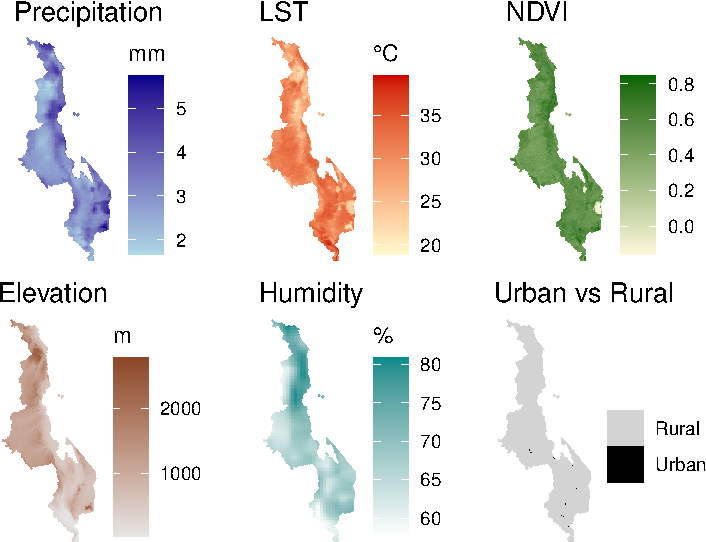
\includegraphics[keepaspectratio]{05_case-studies_files/figure-pdf/fig-covariates-map-1.pdf}}

}

\caption{\label{fig-covariates-map}Raster maps of environmental
covariates extracted from Google Earth Engine for Malawi in 2006. Each
panel shows one covariate: precipitation, land surface temperature
(LST), vegetation cover (NDVI), elevation, relative humidity, and
urbanicity. These layers are used as predictors in the geostatistical
modelling of malaria prevalence.}

\end{figure}%

\subsection{Exploratory analysis}\label{exploratory-analysis-2}

To investigate how \emph{Plasmodium falciparum} prevalence varies with
environmental conditions, we begin by computing the empirical logit
transformation of the observed prevalence at each survey location. Each
covariate is then explored in relation to the empirical logit using
scatterplots. For continuous covariates, we produce scatter plots with
two fitted curves: a LOESS smoother shown in red, and a linear spline
model with a single change point shown in blue. The LOESS curve serves
as a flexible, nonparametric reference for assessing the general trend
in the data. The spline model provides a simple parametric approximation
to this trend, with the change point selected based on visual inspection
of where the LOESS curve departs from linearity.

\begin{Shaded}
\begin{Highlighting}[]

\CommentTok{\# 1. Prepare data}
\NormalTok{mlw\_sf }\OtherTok{\textless{}{-}}\NormalTok{ mlw\_sf }\SpecialCharTok{\%\textgreater{}\%}
  \FunctionTok{mutate}\NormalTok{(}
    \AttributeTok{elogit =} \FunctionTok{log}\NormalTok{((positive }\SpecialCharTok{+} \FloatTok{0.5}\NormalTok{) }\SpecialCharTok{/}\NormalTok{ (examined }\SpecialCharTok{{-}}\NormalTok{ positive }\SpecialCharTok{+} \FloatTok{0.5}\NormalTok{)),}
    \StringTok{\textasciigrave{}}\AttributeTok{Precipitation}\StringTok{\textasciigrave{}} \OtherTok{=}\NormalTok{ precip,}
    \StringTok{\textasciigrave{}}\AttributeTok{Temperature (°C)}\StringTok{\textasciigrave{}} \OtherTok{=}\NormalTok{ lst\_c,}
    \StringTok{\textasciigrave{}}\AttributeTok{NDVI}\StringTok{\textasciigrave{}} \OtherTok{=}\NormalTok{ ndvi,}
    \StringTok{\textasciigrave{}}\AttributeTok{Elevation (m)}\StringTok{\textasciigrave{}} \OtherTok{=}\NormalTok{ elev,}
    \StringTok{\textasciigrave{}}\AttributeTok{Humidity (\%)}\StringTok{\textasciigrave{}} \OtherTok{=}\NormalTok{ humidity,}
    \StringTok{\textasciigrave{}}\AttributeTok{Urbanicity}\StringTok{\textasciigrave{}} \OtherTok{=} \FunctionTok{factor}\NormalTok{(built\_up, }\AttributeTok{levels =} \FunctionTok{c}\NormalTok{(}\DecValTok{0}\NormalTok{, }\DecValTok{1}\NormalTok{), }\AttributeTok{labels =} \FunctionTok{c}\NormalTok{(}\StringTok{"Rural"}\NormalTok{, }\StringTok{"Urban"}\NormalTok{))}
\NormalTok{  )}

\CommentTok{\# 2. Drop geometry and reshape}
\NormalTok{plot\_data\_cont }\OtherTok{\textless{}{-}}\NormalTok{ mlw\_sf }\SpecialCharTok{\%\textgreater{}\%}
  \FunctionTok{select}\NormalTok{(elogit, }\StringTok{\textasciigrave{}}\AttributeTok{Precipitation}\StringTok{\textasciigrave{}}\NormalTok{, }\StringTok{\textasciigrave{}}\AttributeTok{Temperature (°C)}\StringTok{\textasciigrave{}}\NormalTok{, }\StringTok{\textasciigrave{}}\AttributeTok{NDVI}\StringTok{\textasciigrave{}}\NormalTok{, }\StringTok{\textasciigrave{}}\AttributeTok{Elevation (m)}\StringTok{\textasciigrave{}}\NormalTok{, }\StringTok{\textasciigrave{}}\AttributeTok{Humidity (\%)}\StringTok{\textasciigrave{}}\NormalTok{) }\SpecialCharTok{\%\textgreater{}\%}
  \FunctionTok{st\_drop\_geometry}\NormalTok{() }\SpecialCharTok{\%\textgreater{}\%}
  \FunctionTok{pivot\_longer}\NormalTok{(}\AttributeTok{cols =} \SpecialCharTok{{-}}\NormalTok{elogit, }\AttributeTok{names\_to =} \StringTok{"Covariate"}\NormalTok{, }\AttributeTok{values\_to =} \StringTok{"Value"}\NormalTok{)}

\NormalTok{plot\_data\_cat }\OtherTok{\textless{}{-}}\NormalTok{ mlw\_sf }\SpecialCharTok{\%\textgreater{}\%}
  \FunctionTok{select}\NormalTok{(elogit, Urbanicity) }\SpecialCharTok{\%\textgreater{}\%}
  \FunctionTok{st\_drop\_geometry}\NormalTok{()}

\CommentTok{\# 3. Define change points}
\NormalTok{knots }\OtherTok{\textless{}{-}} \FunctionTok{c}\NormalTok{(}
  \StringTok{"Precipitation"} \OtherTok{=} \ConstantTok{Inf}\NormalTok{,}
  \StringTok{"Temperature (°C)"} \OtherTok{=} \DecValTok{33}\NormalTok{,}
  \StringTok{"NDVI"} \OtherTok{=} \ConstantTok{Inf}\NormalTok{,}
  \StringTok{"Elevation (m)"} \OtherTok{=} \DecValTok{400}\NormalTok{,}
  \StringTok{"Humidity (\%)"} \OtherTok{=} \DecValTok{65}
\NormalTok{)}

\CommentTok{\# 4. Create individual continuous plots}
\NormalTok{plots }\OtherTok{\textless{}{-}} \FunctionTok{lapply}\NormalTok{(}\FunctionTok{split}\NormalTok{(plot\_data\_cont, plot\_data\_cont}\SpecialCharTok{$}\NormalTok{Covariate), }\ControlFlowTok{function}\NormalTok{(df) \{}
\NormalTok{  var }\OtherTok{\textless{}{-}} \FunctionTok{unique}\NormalTok{(df}\SpecialCharTok{$}\NormalTok{Covariate)}
\NormalTok{  knot }\OtherTok{\textless{}{-}}\NormalTok{ knots[[var]]}
  
\NormalTok{  df }\OtherTok{\textless{}{-}}\NormalTok{ df }\SpecialCharTok{\%\textgreater{}\%}
    \FunctionTok{mutate}\NormalTok{(}
      \AttributeTok{linear\_part =}\NormalTok{ Value,}
      \AttributeTok{spline\_part =} \FunctionTok{pmax}\NormalTok{(Value }\SpecialCharTok{{-}}\NormalTok{ knot, }\DecValTok{0}\NormalTok{)}
\NormalTok{    )}
  
  \FunctionTok{ggplot}\NormalTok{(df, }\FunctionTok{aes}\NormalTok{(}\AttributeTok{x =}\NormalTok{ Value, }\AttributeTok{y =}\NormalTok{ elogit)) }\SpecialCharTok{+}
    \FunctionTok{geom\_point}\NormalTok{(}\AttributeTok{alpha =} \FloatTok{0.5}\NormalTok{, }\AttributeTok{size =} \DecValTok{1}\NormalTok{) }\SpecialCharTok{+}
    \FunctionTok{geom\_smooth}\NormalTok{(}\AttributeTok{method =} \StringTok{"loess"}\NormalTok{, }\AttributeTok{se =} \ConstantTok{FALSE}\NormalTok{, }\AttributeTok{color =} \StringTok{"red"}\NormalTok{, }\AttributeTok{linewidth =} \DecValTok{1}\NormalTok{) }\SpecialCharTok{+}
    \FunctionTok{geom\_smooth}\NormalTok{(}\AttributeTok{method =} \StringTok{"lm"}\NormalTok{,}
                \AttributeTok{formula =}\NormalTok{ y }\SpecialCharTok{\textasciitilde{}}\NormalTok{ x }\SpecialCharTok{+} \FunctionTok{pmax}\NormalTok{(x }\SpecialCharTok{{-}}\NormalTok{ knot, }\DecValTok{0}\NormalTok{),}
                \AttributeTok{se =} \ConstantTok{FALSE}\NormalTok{, }\AttributeTok{color =} \StringTok{"blue"}\NormalTok{, }\AttributeTok{linewidth =} \DecValTok{1}\NormalTok{) }\SpecialCharTok{+}
    \FunctionTok{labs}\NormalTok{(}\AttributeTok{x =}\NormalTok{ var, }\AttributeTok{y =} \ConstantTok{NULL}\NormalTok{) }\SpecialCharTok{+}
    \FunctionTok{theme\_minimal}\NormalTok{()}
\NormalTok{\})}

\CommentTok{\# 5. Add Urbanicity boxplot}
\NormalTok{p\_urban }\OtherTok{\textless{}{-}} \FunctionTok{ggplot}\NormalTok{(plot\_data\_cat, }\FunctionTok{aes}\NormalTok{(}\AttributeTok{x =}\NormalTok{ Urbanicity, }\AttributeTok{y =}\NormalTok{ elogit)) }\SpecialCharTok{+}
  \FunctionTok{geom\_boxplot}\NormalTok{(}\AttributeTok{outlier.size =} \FloatTok{0.5}\NormalTok{) }\SpecialCharTok{+}
  \FunctionTok{labs}\NormalTok{(}\AttributeTok{x =} \StringTok{"Urbanicity"}\NormalTok{, }\AttributeTok{y =} \ConstantTok{NULL}\NormalTok{) }\SpecialCharTok{+}
  \FunctionTok{theme\_minimal}\NormalTok{()}

\CommentTok{\# 6. Assemble 2 x 3 plot grid}
\NormalTok{final\_plot }\OtherTok{\textless{}{-}}\NormalTok{ (plots[[}\DecValTok{1}\NormalTok{]] }\SpecialCharTok{|}\NormalTok{ plots[[}\DecValTok{2}\NormalTok{]] }\SpecialCharTok{|}\NormalTok{ plots[[}\DecValTok{3}\NormalTok{]]) }\SpecialCharTok{/}
\NormalTok{  (plots[[}\DecValTok{4}\NormalTok{]] }\SpecialCharTok{|}\NormalTok{ plots[[}\DecValTok{5}\NormalTok{]] }\SpecialCharTok{|}\NormalTok{ p\_urban) }\SpecialCharTok{+}
  \FunctionTok{plot\_annotation}\NormalTok{(}\AttributeTok{title =} \StringTok{"Empirical logit of prevalence vs environmental covariates"}\NormalTok{)}

\NormalTok{final\_plot}
\end{Highlighting}
\end{Shaded}

\begin{figure}[H]

\centering{

\pandocbounded{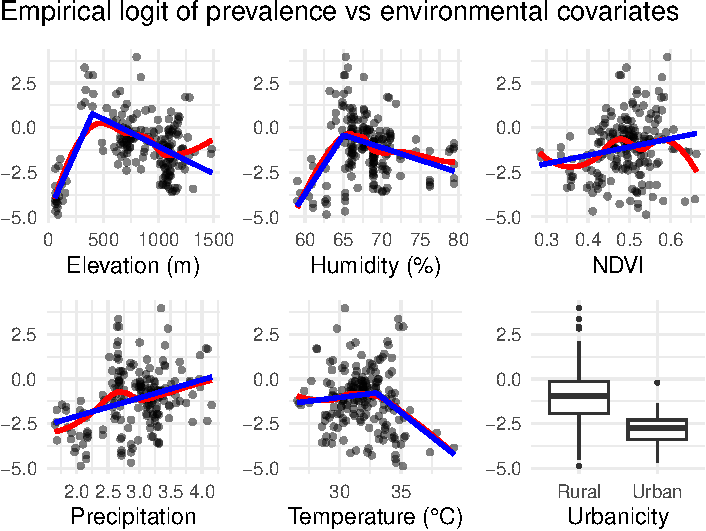
\includegraphics[keepaspectratio]{05_case-studies_files/figure-pdf/fig-elogit-vs-covariates-1.pdf}}

}

\caption{\label{fig-elogit-vs-covariates}Exploratory plots showing the
relationship between the empirical logit of \emph{P. falciparum}
prevalence and the chosen environmental covariates. Scatter plots show
continuous covariates with LOESS (red) and linear spline (blue) fits. A
boxplot is used for the binary urbanicity variable. Change points for
splines are based on graphical inspection of the LOESS fitted
relationship.}

\end{figure}%

Figure~\ref{fig-elogit-vs-covariates} shows the results of this
exploratory approach for the relationship between prevalence and
covariates. For some variables, such as temperature, elevation, and
humidity, there is a clear nonlinear association that is reasonably
captured by a single change point. For others, including precipitation
and NDVI, the relationship appears approximately linear, and for this
reason no change point is used in the spline fit.

Urbanicity is treated separately as a binary covariate and visualized
with a boxplot comparing the empirical logit of prevalence between rural
and urban settings. The boxplot indicates that, as we expect, the level
of prevalence in urban areas is considerable lower than in rural areas.

To assess the degree of correlation between covariates, we compute the
pairwise Pearson correlation coefficients among the continuous
environmental variables.

\begin{Shaded}
\begin{Highlighting}[]
\FunctionTok{library}\NormalTok{(ggcorrplot)}

\CommentTok{\# Select continuous covariates only}
\NormalTok{cont\_vars }\OtherTok{\textless{}{-}}\NormalTok{ mlw\_sf }\SpecialCharTok{\%\textgreater{}\%}
  \FunctionTok{st\_drop\_geometry}\NormalTok{() }\SpecialCharTok{\%\textgreater{}\%}
  \FunctionTok{select}\NormalTok{(}\AttributeTok{Precipitation =}\NormalTok{ precip,}
         \AttributeTok{Temperature =}\NormalTok{ lst\_c,}
         \AttributeTok{NDVI =}\NormalTok{ ndvi,}
         \AttributeTok{Elevation =}\NormalTok{ elev,}
         \AttributeTok{Humidity =}\NormalTok{ humidity)}

\CommentTok{\# Compute correlation matrix}
\NormalTok{corr\_mat }\OtherTok{\textless{}{-}} \FunctionTok{cor}\NormalTok{(cont\_vars, }\AttributeTok{use =} \StringTok{"complete.obs"}\NormalTok{)}

\CommentTok{\# Plot correlation matrix}
\FunctionTok{ggcorrplot}\NormalTok{(corr\_mat,}
           \AttributeTok{method =} \StringTok{"circle"}\NormalTok{,}
           \AttributeTok{type =} \StringTok{"lower"}\NormalTok{,}
           \AttributeTok{lab =} \ConstantTok{TRUE}\NormalTok{,}
           \AttributeTok{lab\_size =} \DecValTok{3}\NormalTok{,}
           \AttributeTok{colors =} \FunctionTok{c}\NormalTok{(}\StringTok{"blue"}\NormalTok{, }\StringTok{"white"}\NormalTok{, }\StringTok{"red"}\NormalTok{),}
           \AttributeTok{title =} \StringTok{"Correlation between covariates"}\NormalTok{,}
           \AttributeTok{ggtheme =} \FunctionTok{theme\_minimal}\NormalTok{())}
\end{Highlighting}
\end{Shaded}

\begin{figure}[H]

\centering{

\pandocbounded{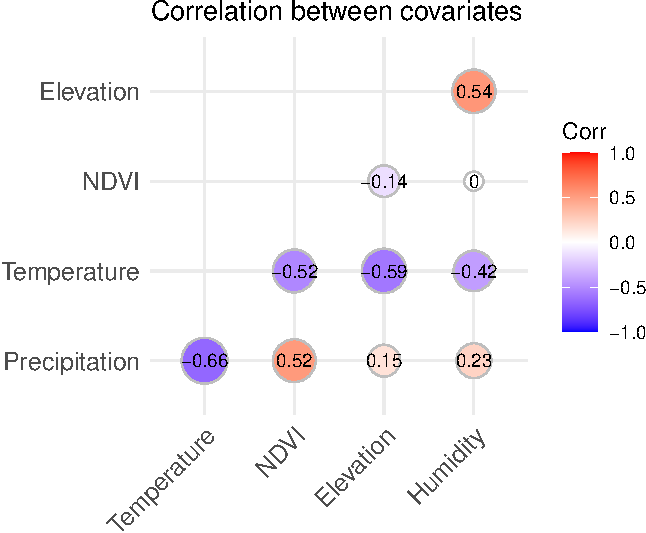
\includegraphics[keepaspectratio]{05_case-studies_files/figure-pdf/fig-correlation-heatmap-1.pdf}}

}

\caption{\label{fig-correlation-heatmap}Pairwise Pearson correlation
matrix between continuous environmental covariates.}

\end{figure}%

The correlations, shown in Figure~Figure~\ref{fig-correlation-heatmap},
are generally moderate in magnitude, ranging from --0.66 between
temperature and precipitation to 0.54 between elevation and relative
humidity. These values indicate that collinearity is not a major concern
in our model development. Each covariate is likely to provide
complementary information about malaria risk, and the absence of strong
dependencies also supports the reliability of the scatterplots used to
explore their individual relationships with prevalence.

We also perform a principal component analysis (PCA) on the standardized
continuous environmental covariates to assess the potential for reducing
dimensionality in our model. The code below shows the implementation of
the PCA.

\begin{Shaded}
\begin{Highlighting}[]
\FunctionTok{library}\NormalTok{(factoextra)}

\CommentTok{\# Prepare only continuous covariates and standardize}
\NormalTok{pca\_data }\OtherTok{\textless{}{-}}\NormalTok{ mlw\_sf }\SpecialCharTok{\%\textgreater{}\%}
  \FunctionTok{st\_drop\_geometry}\NormalTok{() }\SpecialCharTok{\%\textgreater{}\%}
  \FunctionTok{select}\NormalTok{(}\AttributeTok{Precipitation =}\NormalTok{ precip,}
         \AttributeTok{Temperature =}\NormalTok{ lst\_c,}
         \AttributeTok{NDVI =}\NormalTok{ ndvi,}
         \AttributeTok{Elevation =}\NormalTok{ elev,}
         \AttributeTok{Humidity =}\NormalTok{ humidity) }\SpecialCharTok{\%\textgreater{}\%}
  \FunctionTok{scale}\NormalTok{()}

\CommentTok{\# Perform PCA}
\NormalTok{pca\_result }\OtherTok{\textless{}{-}} \FunctionTok{prcomp}\NormalTok{(pca\_data)}

\CommentTok{\# Scree plot}
\FunctionTok{fviz\_eig}\NormalTok{(pca\_result, }\AttributeTok{addlabels =} \ConstantTok{TRUE}\NormalTok{, }\AttributeTok{barfill =} \StringTok{"steelblue"}\NormalTok{, }\AttributeTok{barcolor =} \StringTok{"grey30"}\NormalTok{) }\SpecialCharTok{+}
  \FunctionTok{theme\_minimal}\NormalTok{()}
\end{Highlighting}
\end{Shaded}

\begin{figure}[H]

\centering{

\pandocbounded{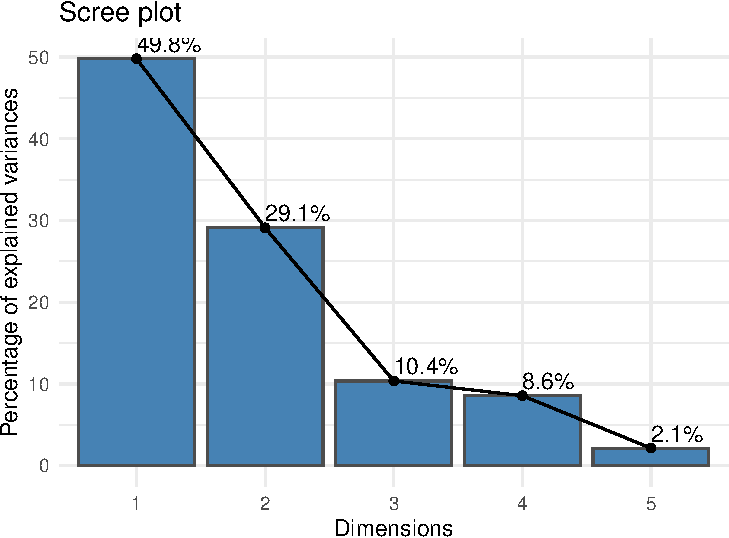
\includegraphics[keepaspectratio]{05_case-studies_files/figure-pdf/fig-pca-scree-1.pdf}}

}

\caption{\label{fig-pca-scree}Proportion of variance explained by the
principal components computed from standardized continuous environmental
covariates.}

\end{figure}%

The scree plot in Figure~Figure~\ref{fig-pca-scree} shows the proportion
of variance explained by each principal component. The first principal
component (PC1) explains approximately 50\% of the total variation,
suggesting it captures a substantial environmental gradient across the
study region. Although additional components may carry useful
information, PC1 stands out as a potential candidate for use in model
building as a composite environmental index and spatial predictor of
malaria prevalence.

\begin{longtable}[]{@{}lcc@{}}

\caption{\label{tbl-pca-loadings}Loadings of the first two principal
components. Each value indicates the contribution of a standardized
covariate to the corresponding component.}

\tabularnewline

\toprule\noalign{}
Covariate & PC1 & PC2 \\
\midrule\noalign{}
\endhead
\bottomrule\noalign{}
\endlastfoot
Precipitation & -0.480 & -0.339 \\
Temperature & 0.596 & 0.043 \\
NDVI & -0.338 & -0.605 \\
Elevation & -0.391 & 0.560 \\
Humidity & -0.385 & 0.451 \\

\end{longtable}

Table~Table~\ref{tbl-pca-loadings} displays the loadings of the first
two principal components. The sign and magnitude of each loading reflect
how much each standardized covariate contributes to the corresponding
component. PC1 shows strong positive loading for temperature and strong
negative loadings for precipitation, humidity, and elevation. This
suggests that PC1 represents a gradient from cool, humid, high-elevation
areas with more rainfall to hotter, drier lowland regions. NDVI also
contributes negatively, implying more vegetation cover in cooler, wetter
zones. We can thus interpret PC1 as a general heat-aridity gradient,
which well aligns with known ecological drivers of malaria risk.

\begin{Shaded}
\begin{Highlighting}[]
\CommentTok{\# Create raster for PC1}
\NormalTok{r\_stack\_std }\OtherTok{\textless{}{-}} \FunctionTok{scale}\NormalTok{(r\_covs[[}\FunctionTok{c}\NormalTok{(}\StringTok{"precip"}\NormalTok{, }\StringTok{"lst\_c"}\NormalTok{, }\StringTok{"ndvi"}\NormalTok{, }\StringTok{"elev"}\NormalTok{, }\StringTok{"humidity"}\NormalTok{)]])}
\NormalTok{pc1\_weights }\OtherTok{\textless{}{-}} \FunctionTok{c}\NormalTok{(}\SpecialCharTok{{-}}\FloatTok{0.480}\NormalTok{, }\FloatTok{0.596}\NormalTok{, }\SpecialCharTok{{-}}\FloatTok{0.338}\NormalTok{, }\SpecialCharTok{{-}}\FloatTok{0.391}\NormalTok{, }\SpecialCharTok{{-}}\FloatTok{0.385}\NormalTok{)}
\NormalTok{pc1\_rast }\OtherTok{\textless{}{-}} \FunctionTok{sum}\NormalTok{(r\_stack\_std }\SpecialCharTok{*}\NormalTok{ pc1\_weights)}
\FunctionTok{names}\NormalTok{(pc1\_rast) }\OtherTok{\textless{}{-}} \StringTok{"PC1"}

\CommentTok{\# Extract PC1 values}
\NormalTok{pc1\_vals }\OtherTok{\textless{}{-}}\NormalTok{ terra}\SpecialCharTok{::}\FunctionTok{extract}\NormalTok{(pc1\_rast, }\FunctionTok{vect}\NormalTok{(mlw\_sf))}
\NormalTok{mlw\_sf}\SpecialCharTok{$}\NormalTok{PC1 }\OtherTok{\textless{}{-}}\NormalTok{ pc1\_vals[, }\DecValTok{2}\NormalTok{]}

\CommentTok{\# Convert raster to df for ggplot}
\NormalTok{pc1\_df }\OtherTok{\textless{}{-}} \FunctionTok{as.data.frame}\NormalTok{(pc1\_rast, }\AttributeTok{xy =} \ConstantTok{TRUE}\NormalTok{, }\AttributeTok{na.rm =} \ConstantTok{TRUE}\NormalTok{)}
\FunctionTok{names}\NormalTok{(pc1\_df) }\OtherTok{\textless{}{-}} \FunctionTok{c}\NormalTok{(}\StringTok{"x"}\NormalTok{, }\StringTok{"y"}\NormalTok{, }\StringTok{"PC1"}\NormalTok{)}

\CommentTok{\# {-}{-}{-} Create PC1 map plot {-}{-}{-}}
\NormalTok{p\_map }\OtherTok{\textless{}{-}} \FunctionTok{ggplot}\NormalTok{(pc1\_df, }\FunctionTok{aes}\NormalTok{(}\AttributeTok{x =}\NormalTok{ x, }\AttributeTok{y =}\NormalTok{ y, }\AttributeTok{fill =}\NormalTok{ PC1)) }\SpecialCharTok{+}
  \FunctionTok{geom\_raster}\NormalTok{() }\SpecialCharTok{+}
  \FunctionTok{scale\_fill\_viridis\_c}\NormalTok{(}\AttributeTok{option =} \StringTok{"C"}\NormalTok{) }\SpecialCharTok{+}
  \FunctionTok{coord\_equal}\NormalTok{() }\SpecialCharTok{+}
  \FunctionTok{theme\_void}\NormalTok{() }\SpecialCharTok{+}
  \FunctionTok{ggtitle}\NormalTok{(}\StringTok{"PC1: Environmental Gradient"}\NormalTok{)}

\CommentTok{\# {-}{-}{-} Create scatterplot with LOESS and spline {-}{-}{-}}
\NormalTok{knot\_pc1 }\OtherTok{\textless{}{-}} \FloatTok{0.75}
\NormalTok{scatter\_df }\OtherTok{\textless{}{-}}\NormalTok{ mlw\_sf }\SpecialCharTok{\%\textgreater{}\%}
  \FunctionTok{mutate}\NormalTok{(}\AttributeTok{spline\_part =} \FunctionTok{pmax}\NormalTok{(PC1 }\SpecialCharTok{{-}}\NormalTok{ knot\_pc1, }\DecValTok{0}\NormalTok{))}

\NormalTok{p\_scatter }\OtherTok{\textless{}{-}} \FunctionTok{ggplot}\NormalTok{(scatter\_df, }\FunctionTok{aes}\NormalTok{(}\AttributeTok{x =}\NormalTok{ PC1, }\AttributeTok{y =}\NormalTok{ elogit)) }\SpecialCharTok{+}
  \FunctionTok{geom\_point}\NormalTok{(}\AttributeTok{alpha =} \FloatTok{0.5}\NormalTok{, }\AttributeTok{size =} \DecValTok{1}\NormalTok{) }\SpecialCharTok{+}
  \FunctionTok{geom\_smooth}\NormalTok{(}\AttributeTok{method =} \StringTok{"loess"}\NormalTok{, }\AttributeTok{se =} \ConstantTok{FALSE}\NormalTok{, }\AttributeTok{color =} \StringTok{"red"}\NormalTok{, }\AttributeTok{linewidth =} \DecValTok{1}\NormalTok{) }\SpecialCharTok{+}
  \FunctionTok{geom\_smooth}\NormalTok{(}\AttributeTok{method =} \StringTok{"lm"}\NormalTok{, }\AttributeTok{formula =}\NormalTok{ y }\SpecialCharTok{\textasciitilde{}}\NormalTok{ x }\SpecialCharTok{+} \FunctionTok{pmax}\NormalTok{(x }\SpecialCharTok{{-}}\NormalTok{ knot\_pc1, }\DecValTok{0}\NormalTok{),}
              \AttributeTok{se =} \ConstantTok{FALSE}\NormalTok{, }\AttributeTok{color =} \StringTok{"blue"}\NormalTok{, }\AttributeTok{linewidth =} \DecValTok{1}\NormalTok{) }\SpecialCharTok{+}
  \FunctionTok{theme\_minimal}\NormalTok{() }\SpecialCharTok{+}
  \FunctionTok{labs}\NormalTok{(}\AttributeTok{x =} \StringTok{"PC1"}\NormalTok{, }\AttributeTok{y =} \StringTok{"Empirical logit"}\NormalTok{) }\SpecialCharTok{+}
  \FunctionTok{ggtitle}\NormalTok{(}\StringTok{"Empirical logit vs PC1"}\NormalTok{)}

\CommentTok{\# {-}{-}{-} Combine using patchwork {-}{-}{-}}
\CommentTok{\# Also add some margin space}
\NormalTok{p\_map }\OtherTok{\textless{}{-}}\NormalTok{ p\_map }\SpecialCharTok{+} \FunctionTok{theme}\NormalTok{(}\AttributeTok{plot.margin =} \FunctionTok{margin}\NormalTok{(}\AttributeTok{r =} \DecValTok{20}\NormalTok{))}
\NormalTok{p\_scatter }\OtherTok{\textless{}{-}}\NormalTok{ p\_scatter }\SpecialCharTok{+} \FunctionTok{theme}\NormalTok{(}\AttributeTok{plot.margin =} \FunctionTok{margin}\NormalTok{(}\AttributeTok{l =} \DecValTok{20}\NormalTok{))}
\NormalTok{p\_map }\SpecialCharTok{+}\NormalTok{ p\_scatter}
\end{Highlighting}
\end{Shaded}

\begin{figure}[H]

\centering{

\pandocbounded{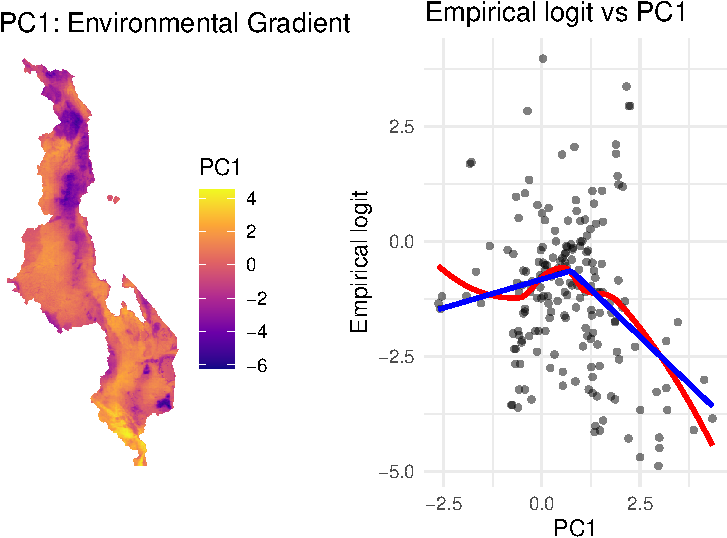
\includegraphics[keepaspectratio]{05_case-studies_files/figure-pdf/fig-pca1-map-scatter-1.pdf}}

}

\caption{\label{fig-pca1-map-scatter}Left: Spatial distribution of the
first principal component (PC1). Right: Empirical logit of malaria
prevalence plotted against PC1 with LOESS (red) and linear spline (blue)
fits.}

\end{figure}%

Figure~\ref{fig-pca1-map-scatter} displays the map of PC1 alongside its
relationship with malaria prevalence. As done previously, to aid
interpretation, we fit a LOESS curve (red) to visualise the general
trend, and a linear spline (blue) with a change point at 0.75 to capture
a simplified parametric relationship. The spline fit suggests a
nonlinear association: malaria risk increases with PC1 up to around
0.75, after which it begins to decline. This pattern implies that
malaria prevalence is highest in areas with intermediate PC1 values,
i.e.~environments that are neither too cold and wet nor too hot and
arid. In other words, there appears to be an optimal range of
environmental conditions, as summarised by PC1, that are most conducive
to malaria transmission. Beyond this range, particularly in more
heat-arid regions, the risk may decline due to ecological constraints on
mosquito survival or parasite development.

In the next section, we compare two modelling approaches. The first
model includes the original environmental covariates using the linear
spline specifications identified during our exploratory analysis. The
second model replaces these covariates with PC1 alone, treating it as a
composite spatial predictor that summarises the dominant environmental
gradient in the study area. In both models, we include urbanicity as a
separate fixed effect. Urbanicity is excluded from the PCA because it is
a binary variable and highly unbalanced, with most survey locations
classified as rural. Modelling it separately ensures that its distinct
contribution to malaria risk, more linked to infrastructure, housing
conditions, and land use, is properly accounted for.

\subsection{Model fitting and spatial
prediction}\label{model-fitting-and-spatial-prediction}

In this section, we fit two geostatistical models to malaria prevalence
data from Malawi, comparing the effects of using separate environmental
covariates versus summarizing them into a principal component.

The first model (\texttt{mod\_all\_cov}) includes all environmental
covariates as separate predictors. Namely these are precipitation
\(d_{\text{prec}}(x)\), NDVI \(d_{\text{ndvi}}(x)\), temperature
\(d_{\text{temp}}(x)\), elevation \(d_{\text{elev}}(x)\), humidity
\(d_{\text{hum}}(x)\), and urbanicity \(d_{\text{urb}}(x)\). Following
from the results of the exploratory analysis, nonlinear effects for
temperature, elevation, and humidity are modeled using linear splines
with thresholds at 33°C, 400\,m, and 65\%, respectively. The
logit-linear model is:

\[
\begin{aligned}
\log\left\{\frac{p(x)}{1 - p(x)}\right\} =\; & 
\beta_0 + 
\beta_1 d_{\text{prec}}(x) +
\beta_2 d_{\text{ndvi}}(x) +
\beta_3 d_{\text{temp}}(x) + \beta_4 \max\{d_{\text{temp}}(x) - 33,\; 0\} \\\\
& +
\beta_5 d_{\text{elev}}(x) + \beta_6 \max\{d_{\text{elev}}(x) - 400,\; 0\} \\\\
& +
\beta_7 d_{\text{hum}}(x) + \beta_8 \max\{d_{\text{hum}}(x) - 65,\; 0\} \\\\
& +
\beta_9 d_{\text{urb}}(x) + S(x)
\end{aligned}
\].

The second model (\texttt{mod\_pca}) replaces the continuous covariates
with their first principal component \(\text{PC}_1(x)\), allowing for a
spline above 0.75. The model becomes:

\[
\log\left\{\frac{p(x)}{1-p(x)}\right\} = \beta_0 + 
\beta_1 \text{PC}_1(x) + 
\beta_2 \max\{\text{PC}_1(x) - 0.75,0\} +
\beta_3 d_{\text{urb}}(x) + S(x)
\]

This formulation allows us to assess whether the dimensionality
reduction via PCA retains the essential variation in environmental risk
while simplifying the model structure.

\begin{Shaded}
\begin{Highlighting}[]
\CommentTok{\# Model with all the covariates as separate predictors}
\NormalTok{mod\_all\_cov }\OtherTok{\textless{}{-}}
\FunctionTok{glgpm}\NormalTok{(positive }\SpecialCharTok{\textasciitilde{}}
\NormalTok{    precip }\SpecialCharTok{+}
\NormalTok{    ndvi }\SpecialCharTok{+}
\NormalTok{    lst\_c }\SpecialCharTok{+} \FunctionTok{pmax}\NormalTok{(lst\_c }\SpecialCharTok{{-}} \DecValTok{33}\NormalTok{, }\DecValTok{0}\NormalTok{) }\SpecialCharTok{+}
\NormalTok{    elev }\SpecialCharTok{+} \FunctionTok{pmax}\NormalTok{(elev }\SpecialCharTok{{-}} \DecValTok{400}\NormalTok{, }\DecValTok{0}\NormalTok{) }\SpecialCharTok{+}
\NormalTok{    humidity }\SpecialCharTok{+} \FunctionTok{pmax}\NormalTok{(humidity }\SpecialCharTok{{-}} \DecValTok{65}\NormalTok{, }\DecValTok{0}\NormalTok{) }\SpecialCharTok{+}
\NormalTok{    built\_up }\SpecialCharTok{+} \FunctionTok{gp}\NormalTok{(),}
    \AttributeTok{den =}\NormalTok{ examined,}
    \AttributeTok{data =}\NormalTok{ mlw\_sf,}
    \AttributeTok{family =} \StringTok{"binomial"}\NormalTok{)}

\CommentTok{\# Model with all the covariates (except \textasciigrave{}built\_up\textasciigrave{})}
\CommentTok{\# combined into PC1 which is then used as predictor}
\NormalTok{mod\_pca }\OtherTok{\textless{}{-}}
  \FunctionTok{glgpm}\NormalTok{(positive }\SpecialCharTok{\textasciitilde{}}
\NormalTok{          PC1 }\SpecialCharTok{+} \FunctionTok{pmax}\NormalTok{(PC1 }\SpecialCharTok{{-}} \FloatTok{0.75}\NormalTok{, }\DecValTok{0}\NormalTok{) }\SpecialCharTok{+}
\NormalTok{          built\_up }\SpecialCharTok{+} \FunctionTok{gp}\NormalTok{(),}
        \AttributeTok{den =}\NormalTok{ examined,}
        \AttributeTok{data =}\NormalTok{ mlw\_sf,}
        \AttributeTok{family =} \StringTok{"binomial"}\NormalTok{)}
\end{Highlighting}
\end{Shaded}

After fitting the two models, when can then compare the summaries of the
fits.

\begin{Shaded}
\begin{Highlighting}[]
\FunctionTok{summary}\NormalTok{(mod\_all\_cov)}
\end{Highlighting}
\end{Shaded}

\begin{verbatim}
Call:
glgpm(formula = positive ~ precip + ndvi + lst_c + pmax(lst_c - 
    33, 0) + elev + pmax(elev - 400, 0) + humidity + pmax(humidity - 
    65, 0) + built_up + gp(), data = mlw_sf, family = "binomial", 
    den = examined)

Binomial geostatistical linear model
Link: canonical (logit) 
Inverse link function = 1 / (1 + exp(-x)) 
 
'Lower limit' and 'Upper limit' are the limits of the 95% confidence level intervals

Regression coefficients
                          Estimate Lower limit Upper limit      StdErr  z.value
(Intercept)            -4.1484e+01 -5.4098e+01 -2.8871e+01  6.4356e+00  -6.4461
precip                  3.6000e-01  2.0822e-01  5.1178e-01  7.7441e-02   4.6487
ndvi                    5.1991e+00  4.3228e+00  6.0754e+00  4.4710e-01  11.6285
lst_c                   9.9929e-02  6.9301e-02  1.3056e-01  1.5626e-02   6.3948
pmax(lst_c - 33, 0)     3.0237e-01  2.5342e-01  3.5132e-01  2.4973e-02  12.1076
elev                    1.0984e-02  1.0581e-02  1.1386e-02  2.0527e-04  53.5074
pmax(elev - 400, 0)    -1.1358e-02 -1.1732e-02 -1.0984e-02  1.9088e-04 -59.5030
humidity                4.7098e-01  4.4719e-01  4.9476e-01  1.2135e-02  38.8129
pmax(humidity - 65, 0) -6.8110e-01 -7.0309e-01 -6.5912e-01  1.1217e-02 -60.7232
built_up               -6.8574e-01 -7.4216e-01 -6.2931e-01  2.8788e-02 -23.8200
                         p.value    
(Intercept)            1.148e-10 ***
precip                 3.340e-06 ***
ndvi                   < 2.2e-16 ***
lst_c                  1.607e-10 ***
pmax(lst_c - 33, 0)    < 2.2e-16 ***
elev                   < 2.2e-16 ***
pmax(elev - 400, 0)    < 2.2e-16 ***
humidity               < 2.2e-16 ***
pmax(humidity - 65, 0) < 2.2e-16 ***
built_up               < 2.2e-16 ***
---
Signif. codes:  0 '***' 0.001 '**' 0.01 '*' 0.05 '.' 0.1 ' ' 1

Spatial Gaussian process
Matern covariance parameters (kappa=0.5)
                     Estimate Lower limit Upper limit
Spatial process var.  0.95284     0.91937      0.9875
Spatial corr. scale  15.60594    15.02071     16.2140
Variance of the nugget effect fixed at 0

Log-likelihood: 13.833
\end{verbatim}

\begin{Shaded}
\begin{Highlighting}[]
\FunctionTok{summary}\NormalTok{(mod\_pca)}
\end{Highlighting}
\end{Shaded}

\begin{verbatim}
Call:
glgpm(formula = positive ~ PC1 + pmax(PC1 - 0.75, 0) + built_up + 
    gp(), data = mlw_sf, family = "binomial", den = examined)

Binomial geostatistical linear model
Link: canonical (logit) 
Inverse link function = 1 / (1 + exp(-x)) 
 
'Lower limit' and 'Upper limit' are the limits of the 95% confidence level intervals

Regression coefficients
                     Estimate Lower limit Upper limit    StdErr  z.value
(Intercept)         -0.496575   -0.595285   -0.397866  0.050363  -9.8600
PC1                  0.258180    0.194448    0.321912  0.032517   7.9399
pmax(PC1 - 0.75, 0) -1.076688   -1.170656   -0.982719  0.047944 -22.4572
built_up            -0.542019   -0.654257   -0.429781  0.057265  -9.4650
                      p.value    
(Intercept)         < 2.2e-16 ***
PC1                 2.024e-15 ***
pmax(PC1 - 0.75, 0) < 2.2e-16 ***
built_up            < 2.2e-16 ***
---
Signif. codes:  0 '***' 0.001 '**' 0.01 '*' 0.05 '.' 0.1 ' ' 1

Spatial Gaussian process
Matern covariance parameters (kappa=0.5)
                     Estimate Lower limit Upper limit
Spatial process var.   2.0008      1.7939      2.2316
Spatial corr. scale   30.6995     27.8239     33.8724
Variance of the nugget effect fixed at 0

Log-likelihood: 15.90143
\end{verbatim}

In the output above, we see that, compared to the model using all
covariates as separate predictors, the model including only PC1 exhibits
both a larger estimated spatial correlation scale and higher spatial
variance. This indicates that replacing the original covariates with PC1
captures a smaller proportion of the spatial variation in prevalence,
leaving the spatial Gaussian process to account for more of the
structured residual variability.

We then compare the predicted prevalence from each model using a regular
5 by 5 km grid covering the whole of Malawi, and display the results in
Figure~\ref{fig-pred_models}. The maps show broadly similar spatial
patterns, with both models identifying areas of high and low predicted
prevalence in the southern region of the country. However, these visual
comparisons do not allow us to determine which model performs better. We
address this question in the next stage of the analysis by formally
assessing the calibration and sharpness of the predictions generated by
each model.

\begin{Shaded}
\begin{Highlighting}[]
\CommentTok{\# Create a 5 by 5 regular grid }
\NormalTok{grid\_mlw }\OtherTok{\textless{}{-}} \FunctionTok{create\_grid}\NormalTok{(mlw\_admin0\_sf, }\AttributeTok{spat\_res =} \DecValTok{5}\NormalTok{)}

\CommentTok{\# Extract the covariates over the grid}
\NormalTok{r\_covs }\OtherTok{\textless{}{-}}\NormalTok{ terra}\SpecialCharTok{::}\FunctionTok{project}\NormalTok{(r\_covs, }\FunctionTok{paste0}\NormalTok{(}\StringTok{"epsg:"}\NormalTok{,mlw\_crs))}
\NormalTok{pc1\_rast }\OtherTok{\textless{}{-}}\NormalTok{ terra}\SpecialCharTok{::}\FunctionTok{project}\NormalTok{(pc1\_rast, }\FunctionTok{paste0}\NormalTok{(}\StringTok{"epsg:"}\NormalTok{,mlw\_crs))}

\NormalTok{predictors }\OtherTok{\textless{}{-}} \FunctionTok{cbind}\NormalTok{(terra}\SpecialCharTok{::}\FunctionTok{extract}\NormalTok{(r\_covs,  }\FunctionTok{st\_coordinates}\NormalTok{(grid\_mlw)),}
\NormalTok{                    terra}\SpecialCharTok{::}\FunctionTok{extract}\NormalTok{(pc1\_rast,  }\FunctionTok{st\_coordinates}\NormalTok{(grid\_mlw)))}

\CommentTok{\# Prevalence prediction over the grid for the two fitted models }
\NormalTok{pred\_all\_cov }\OtherTok{\textless{}{-}} \FunctionTok{pred\_over\_grid}\NormalTok{(mod\_all\_cov,}
                               \AttributeTok{grid\_pred =}\NormalTok{ grid\_mlw,}
                               \AttributeTok{predictors =}\NormalTok{ predictors)}

\NormalTok{pred\_pca }\OtherTok{\textless{}{-}} \FunctionTok{pred\_over\_grid}\NormalTok{(mod\_pca,}
                           \AttributeTok{grid\_pred =}\NormalTok{ grid\_mlw,}
                           \AttributeTok{predictors =}\NormalTok{ predictors)}

\NormalTok{pred\_all\_cov\_prev }\OtherTok{\textless{}{-}} \FunctionTok{pred\_target\_grid}\NormalTok{(pred\_all\_cov,}
                                      \AttributeTok{f\_target =} \FunctionTok{list}\NormalTok{(}\AttributeTok{prev =} \ControlFlowTok{function}\NormalTok{(x) }\FunctionTok{exp}\NormalTok{(x)}\SpecialCharTok{/}\NormalTok{(}\DecValTok{1}\SpecialCharTok{+}\FunctionTok{exp}\NormalTok{(x))))}

\NormalTok{pred\_pca\_prev }\OtherTok{\textless{}{-}} \FunctionTok{pred\_target\_grid}\NormalTok{(pred\_pca,}
                             \AttributeTok{f\_target =} \FunctionTok{list}\NormalTok{(}\AttributeTok{prev =} \ControlFlowTok{function}\NormalTok{(x) }\FunctionTok{exp}\NormalTok{(x)}\SpecialCharTok{/}\NormalTok{(}\DecValTok{1}\SpecialCharTok{+}\FunctionTok{exp}\NormalTok{(x))))}
\end{Highlighting}
\end{Shaded}

\begin{Shaded}
\begin{Highlighting}[]
\FunctionTok{par}\NormalTok{(}\AttributeTok{mfrow =} \FunctionTok{c}\NormalTok{(}\DecValTok{1}\NormalTok{,}\DecValTok{2}\NormalTok{))}
\FunctionTok{plot}\NormalTok{(pred\_all\_cov\_prev, }\AttributeTok{which\_target =} \StringTok{"prev"}\NormalTok{, }\AttributeTok{which\_summary =} \StringTok{"mean"}\NormalTok{,}
     \AttributeTok{main =} \StringTok{"Model: \textquotesingle{}all\_cov\textquotesingle{}"}\NormalTok{, }\AttributeTok{range =} \FunctionTok{c}\NormalTok{(}\DecValTok{0}\NormalTok{,}\DecValTok{1}\NormalTok{))}
\FunctionTok{plot}\NormalTok{(pred\_pca\_prev, }\AttributeTok{which\_target =} \StringTok{"prev"}\NormalTok{, }\AttributeTok{which\_summary =} \StringTok{"mean"}\NormalTok{,}
     \AttributeTok{main =} \StringTok{"Model: \textquotesingle{}pca\textquotesingle{}"}\NormalTok{, }\AttributeTok{range =} \FunctionTok{c}\NormalTok{(}\DecValTok{0}\NormalTok{,}\DecValTok{1}\NormalTok{))}
\end{Highlighting}
\end{Shaded}

\begin{figure}[H]

\centering{

\pandocbounded{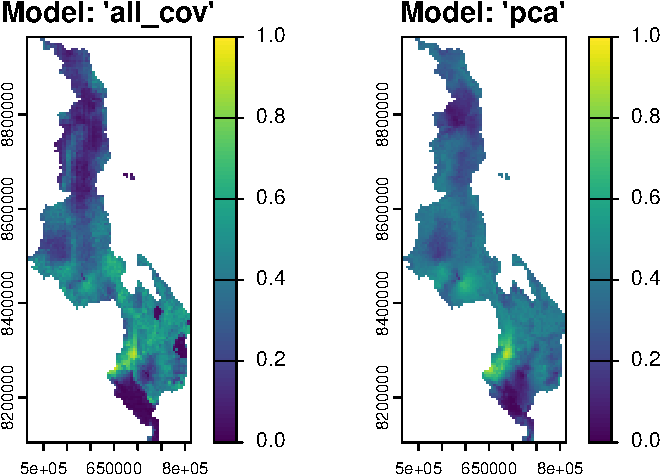
\includegraphics[keepaspectratio]{05_case-studies_files/figure-pdf/fig-pred_models-1.pdf}}

}

\caption{\label{fig-pred_models}Predictive mean of prevalence obtained
from geostatistical models using all covariates (`all\_cov') versus the
first principal component (`pca') of the standardized continuous
environmental variables.}

\end{figure}%

\subsection{Comparison of the predictive performance between
models}\label{comparison-of-the-predictive-performance-between-models}

To evaluate predictive performance, we use three spatially distinct
hold-out test sets corresponding to the Northern, Central, and Southern
regions of Malawi, as illustrated in Figure~\ref{fig-mlw-tests}. These
were constructed using the \texttt{assess\_pp} function with
\texttt{method\ =\ "cluster"} and \texttt{fold\ =\ 3}, ensuring
geographically stratified cross-validation.

\begin{Shaded}
\begin{Highlighting}[]
\NormalTok{assess\_pred\_mlw }\OtherTok{\textless{}{-}}
\FunctionTok{assess\_pp}\NormalTok{(}\FunctionTok{list}\NormalTok{(}\AttributeTok{all\_cov =}\NormalTok{ mod\_all\_cov,}
               \AttributeTok{pca =}\NormalTok{ mod\_pca),}
          \AttributeTok{method =} \StringTok{"cluster"}\NormalTok{,}
          \AttributeTok{which\_metric =} \FunctionTok{c}\NormalTok{(}\StringTok{"AnPIT"}\NormalTok{, }\StringTok{"CRPS"}\NormalTok{),}
          \AttributeTok{iter =} \DecValTok{1}\NormalTok{,}
          \AttributeTok{fold =} \DecValTok{3}\NormalTok{)}
\end{Highlighting}
\end{Shaded}

\begin{figure}

\centering{

\includegraphics[width=0.8\linewidth,height=\textheight,keepaspectratio]{figures/mlw_tests.png}

}

\caption{\label{fig-mlw-tests}Geographic distribution of sampled
locations in Malawi, coloured by their assignment to one of three
cross-validation test sets.}

\end{figure}%

The CRPS score shows that the model including all environmental
covariates achieves better predictive accuracy across all test sets.
Specifically, it yields a lower average CRPS. This improvement is
consistent across the three hold-out data, with particularly notable
gains in Test Set 1. Additionally, the non-randomized probability
integral transform (AnPIT) plot, shown in Figure~\ref{fig-pit-mlw},
demonstrates that the full covariate model is better calibrated: its
cumulative distribution curves lie closer to the identity line,
suggesting that the predicted probabilities align more closely with
observed prevalence.

\begin{Shaded}
\begin{Highlighting}[]
\FunctionTok{plot\_AnPIT}\NormalTok{(assess\_pred\_mlw, }\AttributeTok{mode =} \StringTok{"all"}\NormalTok{)}

\FunctionTok{summary}\NormalTok{(assess\_pred\_mlw)}
\end{Highlighting}
\end{Shaded}

\begin{verbatim}
Summary of Cross-Validation Scores
----------------------------------
Model: all_cov
  Test Set 1:
    CRPS: 1.9452
  Test Set 2:
    CRPS: 2.1383
  Test Set 3:
    CRPS: 1.5148
  Overall average across test sets:
    CRPS: 1.9067

Model: pca
  Test Set 1:
    CRPS: 2.8064
  Test Set 2:
    CRPS: 2.5029
  Test Set 3:
    CRPS: 1.9321
  Overall average across test sets:
    CRPS: 2.6220
\end{verbatim}

\begin{figure}[H]

\centering{

\pandocbounded{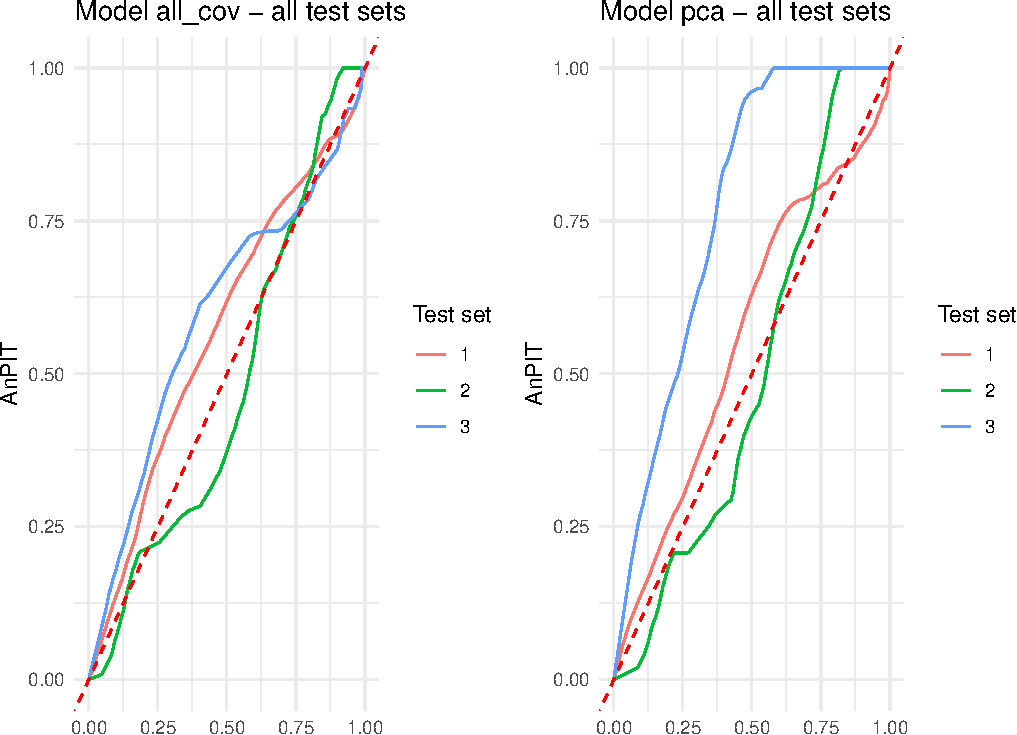
\includegraphics[keepaspectratio]{05_case-studies_files/figure-pdf/fig-pit-mlw-1.pdf}}

}

\caption{\label{fig-pit-mlw}Plot of the average non-randomized
probability integral transform (AnPIT) function to assess the
calibration of the two geostatistical models (`all\_cov' and `pca') for
the malaria prevalence data from Malawi.}

\end{figure}%

\subsection{Summary and conclusions}\label{summary-and-conclusions-1}

In this case study, we have walked through the full pipeline of
conducting a geostatistical analysis of malaria prevalence using Malaria
Indicator Survey data from Malawi. We began by downloading
geo-referenced survey data from the \texttt{malariaAtlas} R package and
retrieving relevant environmental covariates from Google Earth Engine.
These covariates, selected for their mechanistic relevance to malaria
transmission, were processed, clipped to the national boundary, and
extracted at survey locations to be used as predictors in subsequent
modelling.

A critical step in the analysis involved the exploration of
relationships between environmental conditions and malaria prevalence.
Through scatterplots and spline fits, we identified key nonlinearities
in variables such as temperature, elevation, and humidity, which
informed the functional form of covariate effects in the regression
model. This exploratory work is essential not only for model formulation
but also for understanding the ecological underpinnings of disease risk.

To address potential collinearity and reduce the complexity of the
model, we also illustrated the use of PCA as a method for dimensionality
reduction. The first principal component (PC1) captured a dominant
environmental gradient, summarizing variation across temperature,
humidity, elevation, and vegetation, which was then used as a composite
predictor in a reduced model. A simpler alternative is to let the data
guide you through stepwise selection based on p-values---for example,
adding or removing covariates until all retained terms meet a preset
significance threshold. When the pool of candidate predictors is large
relative to the sample size, however, stepwise methods can become
unstable and over-fit; in such cases penalised approaches (e.g.~ridge,
lasso) or resampling-based strategies are usually preferred. A thorough
discussion of these issues, with practical recommendations, is given in
Section 4.7 of Harrell (2015).

We compared two geostatistical models: one using all environmental
covariates as separate predictors (with spline terms for nonlinear
effects), and another using PC1 as a summary predictor. Cross-validation
based on geographically stratified folds revealed that the full model
was better calibrated and achieved sharper predictions, as measured by
lower CRPS and AnPIT curves closer to the identity line.

We encourage the reader to explore Exercise 2 at the end of this
chapter, where you will investigate whether including a second principal
component (PC2) alongside PC1 leads to improved predictive performance.
This offers an opportunity to assess whether PCA-based dimensionality
reduction can match or exceed the predictive accuracy of models that
include all covariates, while potentially offering greater parsimony.

\section{Mapping the vector index for West Nile Virus in the Sacramento
Metropolitan Area, United States}\label{sec-wnv}

In this section, we analyse entomological surveillance data on
\emph{Culex pipiens} in the Sacramento Metropolitan Area (SMA),
California, from 2015 to 2021. \emph{Cx. pipiens} is one of the primary
vectors of West Nile virus (WNV) in North America (Petersen, Brault, and
Nasci 2013; Kramer, Li, and Shi 2007). WNV is a mosquito borne
flavivirus sustained in an enzootic cycle, that is, persistent
circulation of the virus within non human animal populations, primarily
birds, in a defined geographic area. Transmission is maintained between
\emph{Culex} mosquitoes and birds, while humans and other mammals are
incidental dead end hosts that do not contribute to further
transmission. Most human infections are asymptomatic, a minority present
with febrile illness, and a small proportion develop neuroinvasive
disease (Petersen, Brault, and Nasci 2013). Surveillance of both vector
abundance and WNV infection prevalence is therefore important for
anticipating human risk and guiding public health interventions.

In this analysis, we quantify local entomological risk using the vector
index (VI), defined as \begin{equation}\phantomsection\label{eq-vi}{
\text{VI} \;=\; \text{abundance} \times \text{infection prevalence}.  
}\end{equation} Here, \emph{abundance} is the mean number of female
mosquitoes collected per trap night, and \emph{infection prevalence} is
the estimated proportion of mosquitoes infected with WNV in the vector
population. In practice, prevalence is inferred from pooled PCR testing
using maximum likelihood estimators for pooled samples (Centers for
Disease Control and Prevention 2024). Many operational analyses also
report the minimum infection rate and apply either the maximum
likelihood estimate or the minimum infection rate when computing the
vector index (e.g., Bolling et al. 2009; Jones et al. 2011). In this
section, we extend these approaches using model-based geostatistics.

In what follows, we model abundance and infection prevalence for
\emph{Cx. pipiens} as two independent processes and combine the
resulting estimates to obtain VI. We return to this assumption and other
limitations of the analysis in Section~\ref{sec-summary-wnv}.

\subsection{\texorpdfstring{Modelling the abundance of \emph{Culex
pipiens}}{Modelling the abundance of Culex pipiens}}\label{sec-abund-model}

We begin by loading the necessary libraries and the data derived from
the \texttt{vectorsurvR} package in R. The original datasets,
\texttt{sample\_pools} and \texttt{sample\_collections}, contain
mosquito surveillance data from California, including species
identification, collection date, location, pathogen testing results,
trap type, and trapping effort. For this case study, these have been
processed to produce \texttt{abund\_sma} in the \texttt{RiskMap}
package, which summarises the abundance of female \emph{Culex pipiens}
within the Sacramento Metropolitan Area (SMA).

\begin{Shaded}
\begin{Highlighting}[]
\FunctionTok{rm}\NormalTok{(}\AttributeTok{list =} \FunctionTok{ls}\NormalTok{())}

\FunctionTok{library}\NormalTok{(ggplot2)}
\FunctionTok{library}\NormalTok{(patchwork)}

\FunctionTok{data}\NormalTok{(abund\_sma)}
\FunctionTok{str}\NormalTok{(abund\_sma)}
\DocumentationTok{\#\# \textquotesingle{}data.frame\textquotesingle{}:    1551 obs. of  6 variables:}
\DocumentationTok{\#\#  $ lon          : num  {-}121 {-}121 {-}121 {-}121 {-}121 ...}
\DocumentationTok{\#\#  $ lat          : num  38.9 38.8 38.9 38.8 38.9 ...}
\DocumentationTok{\#\#  $ total\_females: int  1 36 6 31 1 1 1 1 1 4 ...}
\DocumentationTok{\#\#  $ date         : Date, format: "2015{-}01{-}02" "2015{-}01{-}02" ...}
\DocumentationTok{\#\#  $ trap\_nights  : int  15 15 15 8 8 8 8 6 6 6 ...}
\DocumentationTok{\#\#  $ trap\_type    : chr  "NJLT" "NJLT" "NJLT" "GRVD" ...}
\end{Highlighting}
\end{Shaded}

The outcome variable for this analysis is \texttt{total\_females}, which
records the total number of \emph{Cx. pipiens} captured in a single
trap. The variable \texttt{trap\_nights} indicates the number of nights
the trap was deployed and is used to account for variation in sampling
effort across traps. The dataset also records the type of trap used
(\texttt{trap\_type}), which can influence capture rates. Trap types
include New Jersey Light Traps (\texttt{NJLT}), Gravid Traps
(\texttt{GRVD}), Mosquito Magnet Traps (\texttt{MMT}), BG-Sentinel Traps
(\texttt{BGSENT}), \(\text{CO}_2\)-baited traps (\texttt{CO2}), Backpack
aspirators (\texttt{BACKPACK}), Lockyer traps (\texttt{LCKR}), and
Ovitraps (\texttt{OVI}). These traps differ in their mode of attraction:
for example, light traps attract host-seeking females using light,
gravid traps target egg-laying females with an infusion lure,
\(\text{CO}_2\)-baited and BG-Sentinel traps mimic host cues through
carbon dioxide and human scent, and backpack or hand-collection methods
are opportunistic. Based on average catch per trap-night, we group these
into low-yield traps (Backpack, Lockyer, New Jersey Light Trap,
Ovitrap), moderate-yield traps (Gravid Trap, Mosquito Magnet), and
high-yield traps (\(\text{CO}_2\)-baited and BG-Sentinel), providing a
more interpretable classification for analysing trap efficiency in
subsequent modelling. We thus create the variable \texttt{trap\_group}
for later use in the model fitting as follows.

\begin{Shaded}
\begin{Highlighting}[]
\NormalTok{abund\_sma }\OtherTok{\textless{}{-}}\NormalTok{ abund\_sma }\SpecialCharTok{\%\textgreater{}\%}
  \FunctionTok{mutate}\NormalTok{(}\AttributeTok{trap\_group =} \FunctionTok{case\_when}\NormalTok{(}
\NormalTok{    trap\_type }\SpecialCharTok{\%in\%} \FunctionTok{c}\NormalTok{(}\StringTok{"BACKPACK"}\NormalTok{, }\StringTok{"LCKR"}\NormalTok{, }\StringTok{"NJLT"}\NormalTok{, }\StringTok{"OVI"}\NormalTok{) }\SpecialCharTok{\textasciitilde{}} \StringTok{"low yeild"}\NormalTok{,}
\NormalTok{    trap\_type }\SpecialCharTok{\%in\%} \FunctionTok{c}\NormalTok{(}\StringTok{"GRVD"}\NormalTok{, }\StringTok{"MMT"}\NormalTok{) }\SpecialCharTok{\textasciitilde{}} \StringTok{"moderate yeild"}\NormalTok{,}
\NormalTok{    trap\_type }\SpecialCharTok{\%in\%} \FunctionTok{c}\NormalTok{(}\StringTok{"CO2"}\NormalTok{, }\StringTok{"BGSENT"}\NormalTok{) }\SpecialCharTok{\textasciitilde{}} \StringTok{"high yield"}
\NormalTok{  ))}
\end{Highlighting}
\end{Shaded}

To provide spatial context, we use the \texttt{rgeoboundaries} package
to download second-level administrative boundaries (ADM2) for the United
States. We extract the boundaries for Placer, El Dorado and Sacrament
counties which make up the SMA.

\begin{Shaded}
\begin{Highlighting}[]
\FunctionTok{library}\NormalTok{(rgeoboundaries)}

\CommentTok{\# Get California ADM2 units and filter to relevant counties}
\NormalTok{ca\_counties }\OtherTok{\textless{}{-}} \FunctionTok{geoboundaries}\NormalTok{(}\StringTok{"United States of America"}\NormalTok{, }\AttributeTok{adm\_lvl =} \StringTok{"ADM2"}\NormalTok{)}
\NormalTok{sma\_names }\OtherTok{\textless{}{-}} \FunctionTok{c}\NormalTok{(}\StringTok{"Sacramento"}\NormalTok{, }\StringTok{"Placer"}\NormalTok{, }\StringTok{"El Dorado"}\NormalTok{)}
\NormalTok{sma\_boundaries }\OtherTok{\textless{}{-}}\NormalTok{ ca\_counties[ca\_counties}\SpecialCharTok{$}\NormalTok{shapeName }\SpecialCharTok{\%in\%}\NormalTok{ sma\_names, ]}
\end{Highlighting}
\end{Shaded}

Given the time span of the data, it is important to consider the
potential for temporal variation in mosquito abundance and infection
prevalence. Changes in environmental conditions, climate, or vector
control efforts may lead to substantial year-to-year fluctuations in
mosquito populations. Additionally, if different geographic areas were
sampled in different years, this could introduce spatial confounding,
making it difficult to disentangle spatial from temporal effects.

The top panel of Figure~\ref{fig-wnv-years} reveals that while some
spatial variation in sampling locations is present across years, there
remains sufficient geographic overlap to enable estimation of temporal
trends in mosquito counts. Overall, \emph{Cx. pipiens} abundance
declines over time, although the trend is more pronounced in high-yield
traps, while moderate- and low-yield traps exhibit a more variable
pattern. The decline in \emph{Cx. pipiens} likely reflects two key
drivers: reduced availability of aquatic breeding sites due to drought,
and intensified vector control efforts. Bhattachan et al. (2023)
reported that \emph{Cx. pipiens} populations in southern California
dropped by about \(40%
\) during the 2012--2016 drought, linked to water-use restrictions that
limited larval habitat in storm drains and catch basins. At the same
time, vector control districts expanded targeted interventions. For
example, the Sacramento--Yolo district treated over 160,000 drains in
2018 alone (Sacramento-Yolo Mosquito and Vector Control District 2018),
and the statewide response plan formalised such practices as part of
integrated mosquito management (California Department of Public Health
2025). For these reasons, our model shall include a covariate for year,
with a log-linear effect on the mean number of \emph{Cx. pipiens}, under
the expectation that abundance will show a decreasing trend over time.

\begin{Shaded}
\begin{Highlighting}[]
\CommentTok{\# Creation of the variable year}
\NormalTok{abund\_sma}\SpecialCharTok{$}\NormalTok{year }\OtherTok{\textless{}{-}} \FunctionTok{as.numeric}\NormalTok{(}\FunctionTok{substr}\NormalTok{(abund\_sma}\SpecialCharTok{$}\NormalTok{date, }\DecValTok{1}\NormalTok{, }\DecValTok{4}\NormalTok{))}

\CommentTok{\# bbox for coord\_sf limits}
\NormalTok{bb }\OtherTok{\textless{}{-}} \FunctionTok{st\_bbox}\NormalTok{(sma\_boundaries)}
\NormalTok{abund\_sma }\OtherTok{\textless{}{-}} \FunctionTok{st\_as\_sf}\NormalTok{(abund\_sma, }\AttributeTok{coords =} \FunctionTok{c}\NormalTok{(}\StringTok{"lon"}\NormalTok{,}\StringTok{"lat"}\NormalTok{), }\AttributeTok{crs =} \DecValTok{4326}\NormalTok{, }\AttributeTok{remove =} \ConstantTok{FALSE}\NormalTok{)}


\CommentTok{\# Panel 1: faceted map, colored by trap\_group (scales fixed!)}
\NormalTok{p\_locs }\OtherTok{\textless{}{-}} \FunctionTok{ggplot}\NormalTok{() }\SpecialCharTok{+}
  \FunctionTok{geom\_sf}\NormalTok{(}\AttributeTok{data =}\NormalTok{ sma\_boundaries, }\AttributeTok{fill =} \ConstantTok{NA}\NormalTok{, }\AttributeTok{color =} \StringTok{"black"}\NormalTok{, }\AttributeTok{linewidth =} \FloatTok{0.3}\NormalTok{) }\SpecialCharTok{+}
  \FunctionTok{geom\_sf}\NormalTok{(}\AttributeTok{data =}\NormalTok{ abund\_sma, }\AttributeTok{color =} \StringTok{"black"}\NormalTok{, }\AttributeTok{alpha =} \FloatTok{0.85}\NormalTok{, }\AttributeTok{size =} \FloatTok{0.9}\NormalTok{) }\SpecialCharTok{+}
  \FunctionTok{coord\_sf}\NormalTok{(}\AttributeTok{xlim =} \FunctionTok{c}\NormalTok{(bb[}\StringTok{"xmin"}\NormalTok{], bb[}\StringTok{"xmax"}\NormalTok{]), }\AttributeTok{ylim =} \FunctionTok{c}\NormalTok{(bb[}\StringTok{"ymin"}\NormalTok{], bb[}\StringTok{"ymax"}\NormalTok{])) }\SpecialCharTok{+}
  \FunctionTok{facet\_wrap}\NormalTok{(}\SpecialCharTok{\textasciitilde{}}\NormalTok{ year, }\AttributeTok{ncol =} \DecValTok{4}\NormalTok{) }\SpecialCharTok{+}
  \FunctionTok{theme\_minimal}\NormalTok{() }\SpecialCharTok{+}
  \FunctionTok{labs}\NormalTok{(}\AttributeTok{title =} \StringTok{"Trap locations by year"}\NormalTok{) }\SpecialCharTok{+}
  \FunctionTok{theme}\NormalTok{(}
    \AttributeTok{strip.text =} \FunctionTok{element\_text}\NormalTok{(}\AttributeTok{size =} \DecValTok{13}\NormalTok{, }\AttributeTok{face =} \StringTok{"bold"}\NormalTok{),}
    \AttributeTok{plot.title =} \FunctionTok{element\_text}\NormalTok{(}\AttributeTok{size =} \DecValTok{16}\NormalTok{, }\AttributeTok{face =} \StringTok{"bold"}\NormalTok{, }\AttributeTok{hjust =} \FloatTok{0.5}\NormalTok{),}
    \AttributeTok{axis.text =} \FunctionTok{element\_blank}\NormalTok{(),}
    \AttributeTok{axis.ticks =} \FunctionTok{element\_blank}\NormalTok{()}
\NormalTok{  )}

\CommentTok{\# Panel 2: average mosquitoes per trap by year \& trap\_group}
\NormalTok{annual\_summary }\OtherTok{\textless{}{-}}\NormalTok{ abund\_sma }\SpecialCharTok{\%\textgreater{}\%}
  \FunctionTok{group\_by}\NormalTok{(year, trap\_group) }\SpecialCharTok{\%\textgreater{}\%}
  \FunctionTok{summarise}\NormalTok{(}
    \AttributeTok{total\_mosquitoes =} \FunctionTok{sum}\NormalTok{(total\_females, }\AttributeTok{na.rm =} \ConstantTok{TRUE}\NormalTok{),}
    \AttributeTok{total\_traps =} \FunctionTok{n}\NormalTok{(),}
    \AttributeTok{mosq\_per\_trap =} \FunctionTok{ifelse}\NormalTok{(total\_traps }\SpecialCharTok{\textgreater{}} \DecValTok{0}\NormalTok{, total\_mosquitoes }\SpecialCharTok{/}\NormalTok{ total\_traps, }\ConstantTok{NA\_real\_}\NormalTok{),}
    \AttributeTok{.groups =} \StringTok{"drop"}
\NormalTok{  )}

\NormalTok{p\_pertrap }\OtherTok{\textless{}{-}} \FunctionTok{ggplot}\NormalTok{(annual\_summary,}
                    \FunctionTok{aes}\NormalTok{(}\AttributeTok{x =} \FunctionTok{factor}\NormalTok{(year), }\AttributeTok{y =}\NormalTok{ mosq\_per\_trap, }\AttributeTok{fill =}\NormalTok{ trap\_group)) }\SpecialCharTok{+}
  \FunctionTok{geom\_col}\NormalTok{(}\AttributeTok{position =} \FunctionTok{position\_dodge}\NormalTok{(}\AttributeTok{width =} \FloatTok{0.7}\NormalTok{), }\AttributeTok{width =} \FloatTok{0.7}\NormalTok{) }\SpecialCharTok{+}
  \FunctionTok{theme\_minimal}\NormalTok{() }\SpecialCharTok{+}
  \FunctionTok{labs}\NormalTok{(}\AttributeTok{title =} \StringTok{"Average mosquitoes per trap by year and trap group"}\NormalTok{,}
       \AttributeTok{x =} \StringTok{"Year"}\NormalTok{, }\AttributeTok{y =} \StringTok{"Mosquitoes per trap"}\NormalTok{, }\AttributeTok{fill =} \StringTok{"Trap group"}\NormalTok{) }\SpecialCharTok{+}
  \FunctionTok{theme}\NormalTok{(}
    \AttributeTok{plot.title =} \FunctionTok{element\_text}\NormalTok{(}\AttributeTok{size =} \DecValTok{14}\NormalTok{, }\AttributeTok{face =} \StringTok{"bold"}\NormalTok{, }\AttributeTok{hjust =} \FloatTok{0.5}\NormalTok{),}
    \AttributeTok{axis.title =} \FunctionTok{element\_text}\NormalTok{(}\AttributeTok{size =} \DecValTok{12}\NormalTok{),}
    \AttributeTok{axis.text =} \FunctionTok{element\_text}\NormalTok{(}\AttributeTok{size =} \DecValTok{11}\NormalTok{)}
\NormalTok{  )}

\CommentTok{\# Combine}
\NormalTok{(p\_locs }\SpecialCharTok{/}\NormalTok{ p\_pertrap) }\SpecialCharTok{+}
  \FunctionTok{plot\_layout}\NormalTok{(}\AttributeTok{heights =} \FunctionTok{c}\NormalTok{(}\DecValTok{3}\NormalTok{, }\DecValTok{1}\NormalTok{))}
\end{Highlighting}
\end{Shaded}

\begin{figure}[H]

\centering{

\pandocbounded{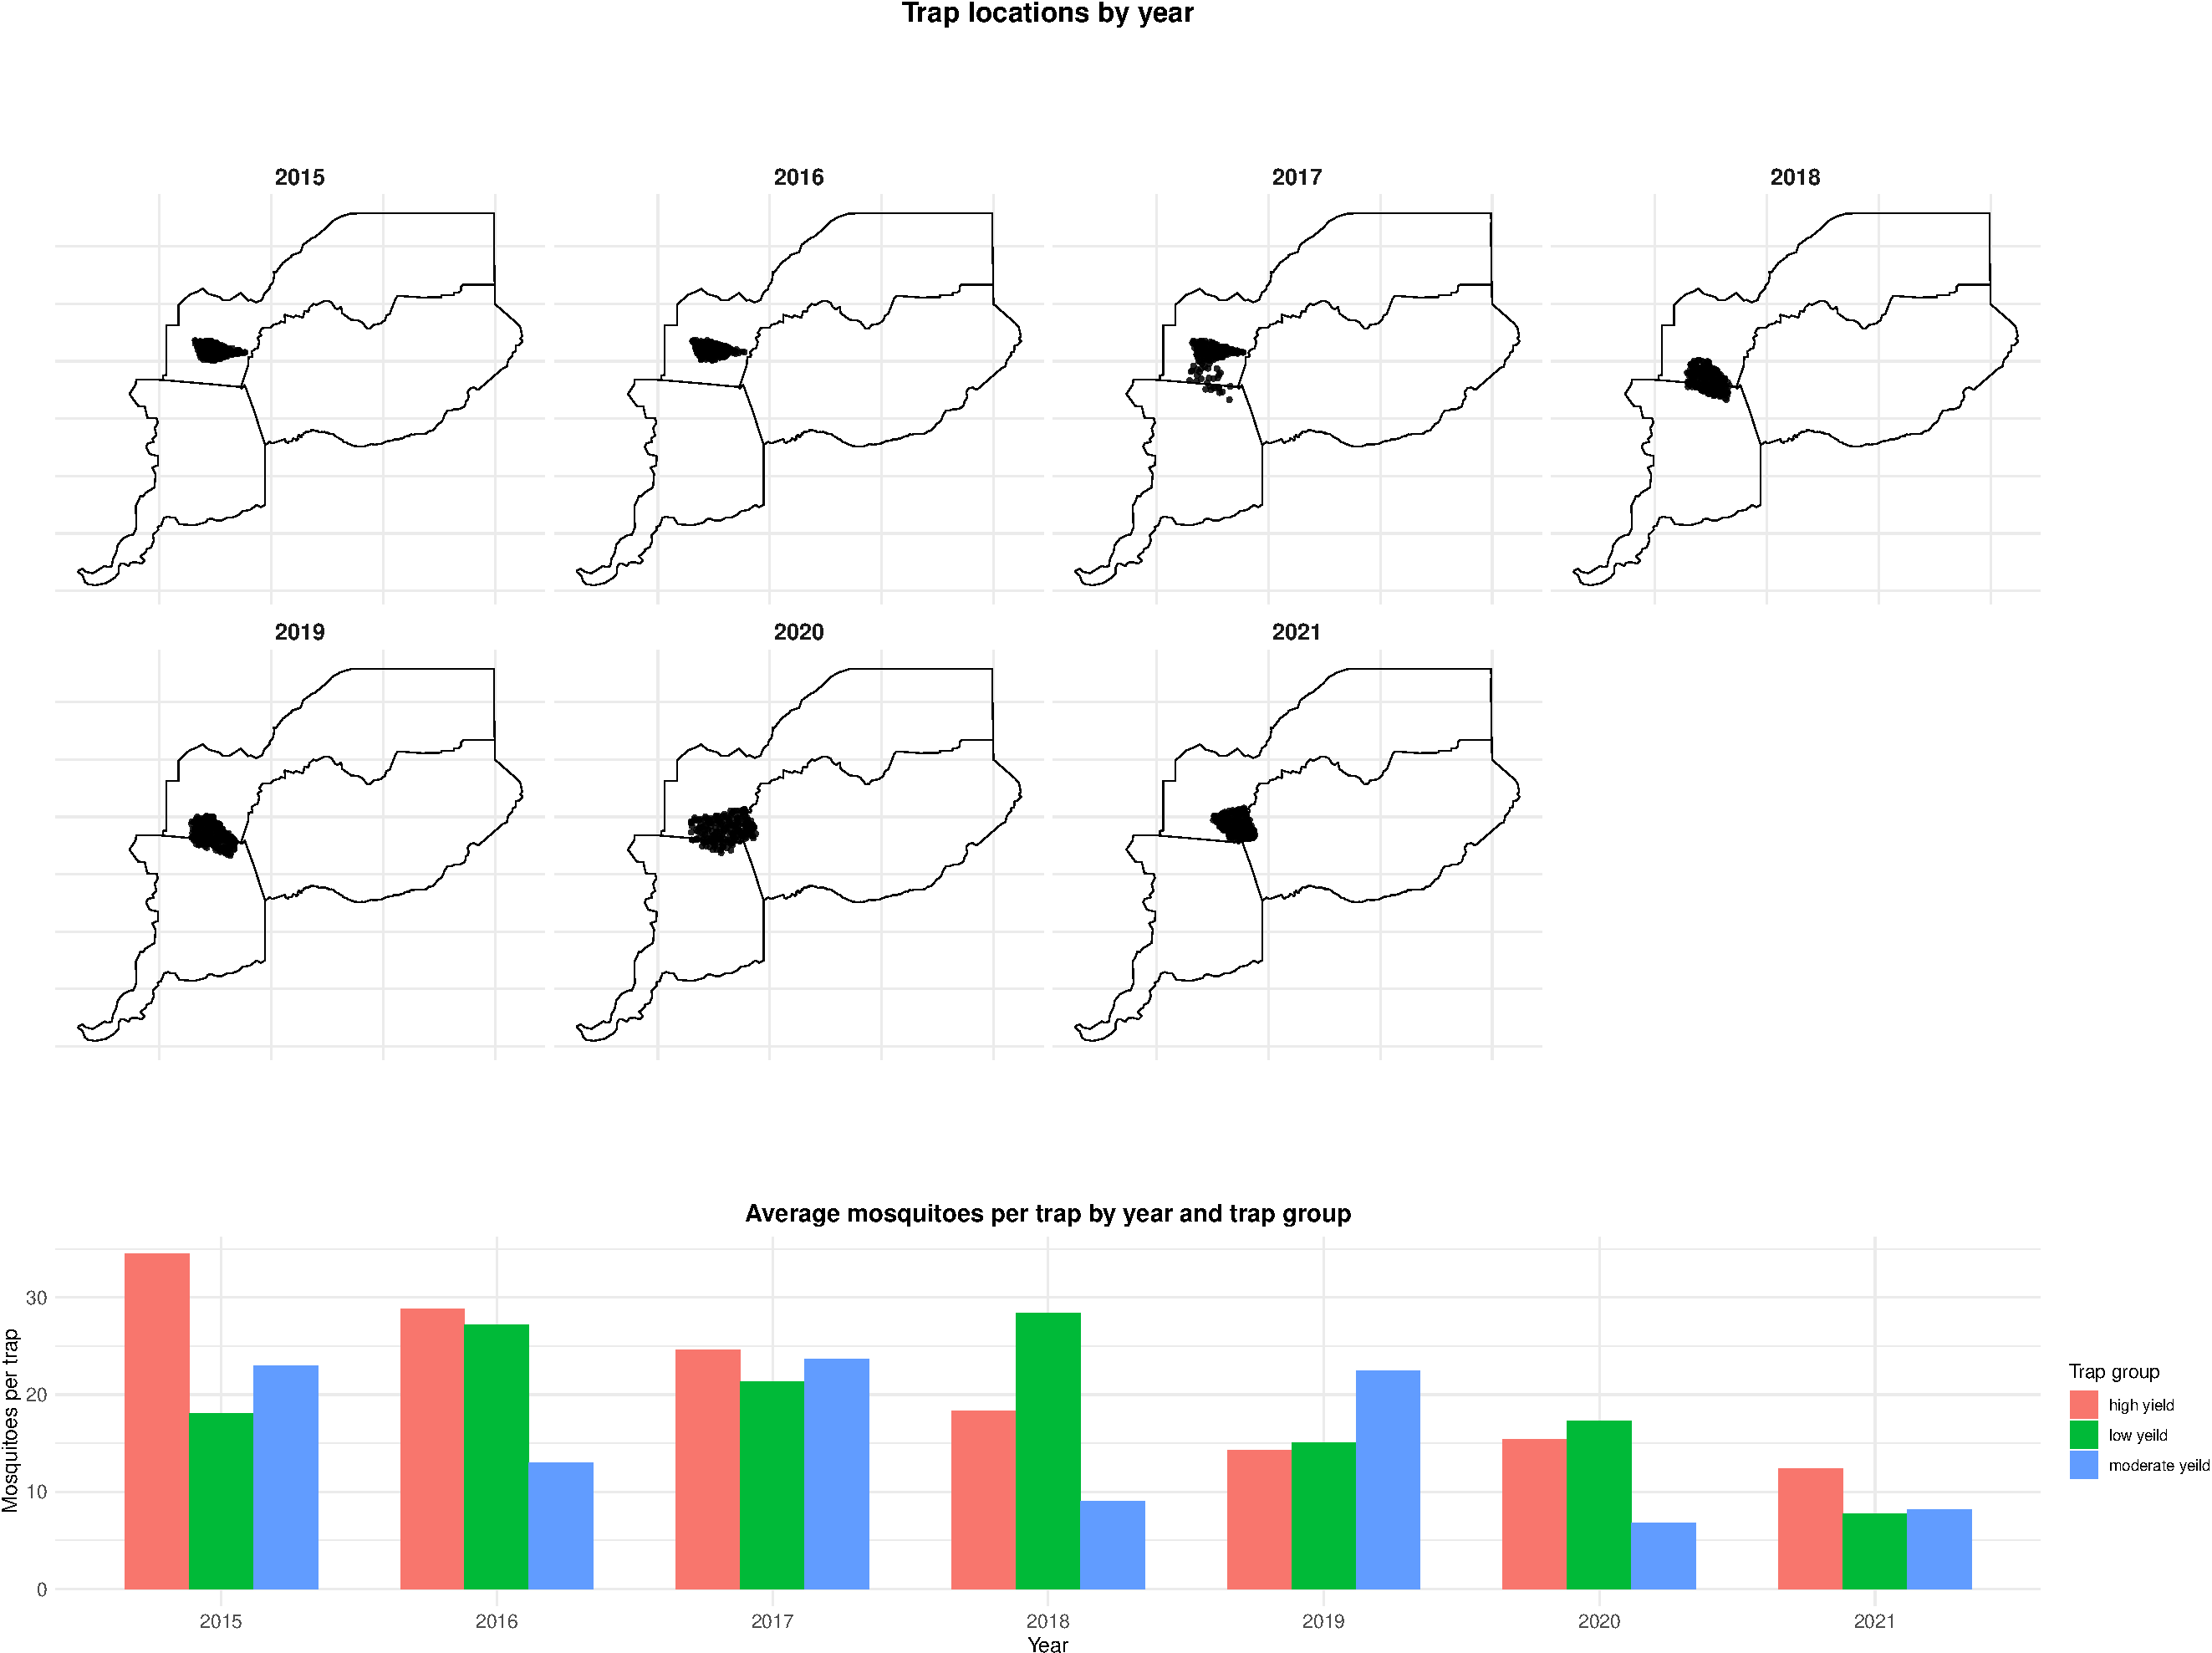
\includegraphics[keepaspectratio]{05_case-studies_files/figure-pdf/fig-wnv-years-1.pdf}}

}

\caption{\label{fig-wnv-years}Spatial and temporal overview of \emph{Cx.
pipiens} surveillance in the Sacramento Metropolitan Area from 2015 to
2021. The top panel shows the spatial distribution of trap locations for
each year. The bottom panel displays the annual average number of
mosquitoes captured per trap by trap group, illustrating variation in
abundance over time.}

\end{figure}%

In our analysis, we first assess whether there is residual spatial
correlation in mosquito counts by fitting the following Poisson
mixed-effects model. Let \(Y_i\) denote the number of trapped female
\emph{Cx. pipiens} at location \(x_i\) and year \(t_i\). Conditionally
on independent and identically distributed zero-mean Gaussian random
effects \(Z_i \sim \mathcal{N}(0, \sigma^2)\), we assume: \[
Y_i \mid Z_i \sim \text{Poisson}(m_i\lambda_i),
\] where \(m_i\) is the number of nights during which the trap has been
deployed, and \(\lambda_i\) is the average number of \(Cx. pipiens\) per
trap-night, which we model as:
\begin{equation}\phantomsection\label{eq-wnv-counts}{
\begin{aligned}
\log\{\lambda_i\} = & 
\sum_{j=1}^3 d_{j}(x_i, t_i) \beta_j + \beta_4 t_i + 
Z_i \\\\
=& \: \mu_i + Z_i,
\end{aligned}
}\end{equation} where the \(d_{j}(x_i, t_i)\) are binary indicators for
the type of trap (\(j=1\) corresponding to ``high-yield'', \(j=2\) to
``moderate-yield'' and \(j=3\) to ``low-yield'') and
\(\mu_i = \sum_{j=1}^3 d_{j}(x_i, t_i) \beta_j + \beta_4 t_i\). We then
fit this model using the \texttt{glmer} function from the \texttt{lme4}
package as follows.

\begin{Shaded}
\begin{Highlighting}[]
\NormalTok{abund\_sma}\SpecialCharTok{$}\NormalTok{loc }\OtherTok{\textless{}{-}} \DecValTok{1}\SpecialCharTok{:}\FunctionTok{nrow}\NormalTok{(abund\_sma)}

\CommentTok{\# In the fit, we scale the variable year to help convergence}
\NormalTok{glmer\_wvn }\OtherTok{\textless{}{-}} \FunctionTok{glmer}\NormalTok{(total\_females }\SpecialCharTok{\textasciitilde{}} \SpecialCharTok{{-}}\DecValTok{1} \SpecialCharTok{+}\NormalTok{ trap\_group }\SpecialCharTok{+} \FunctionTok{scale}\NormalTok{(year) }\SpecialCharTok{+} \FunctionTok{offset}\NormalTok{(}\FunctionTok{log}\NormalTok{(trap\_nights)) }\SpecialCharTok{+}\NormalTok{ (}\DecValTok{1} \SpecialCharTok{|}\NormalTok{ loc),}
                   \AttributeTok{data =}\NormalTok{ abund\_sma, }\AttributeTok{family =}\NormalTok{ poisson,}
                   \AttributeTok{nAGQ =} \DecValTok{100}\NormalTok{)}
\FunctionTok{summary}\NormalTok{(glmer\_wvn)}
\end{Highlighting}
\end{Shaded}

\begin{verbatim}
Generalized linear mixed model fit by maximum likelihood (Adaptive
  Gauss-Hermite Quadrature, nAGQ = 100) [glmerMod]
 Family: poisson  ( log )
Formula: 
total_females ~ -1 + trap_group + scale(year) + offset(log(trap_nights)) +  
    (1 | loc)
   Data: abund_sma

      AIC       BIC    logLik -2*log(L)  df.resid 
   5715.5    5742.2   -2852.7    5705.5      1546 

Scaled residuals: 
     Min       1Q   Median       3Q      Max 
-0.81365 -0.27049 -0.02063  0.10058  0.40034 

Random effects:
 Groups Name        Variance Std.Dev.
 loc    (Intercept) 2.356    1.535   
Number of obs: 1551, groups:  loc, 1551

Fixed effects:
                         Estimate Std. Error z value Pr(>|z|)    
trap_grouphigh yield      1.68272    0.06643  25.331  < 2e-16 ***
trap_grouplow yeild      -0.41146    0.08736  -4.710 2.48e-06 ***
trap_groupmoderate yeild  0.29882    0.06762   4.419 9.92e-06 ***
scale(year)              -0.20370    0.04206  -4.843 1.28e-06 ***
---
Signif. codes:  0 '***' 0.001 '**' 0.01 '*' 0.05 '.' 0.1 ' ' 1

Correlation of Fixed Effects:
            trp_grphy trp_grply trp_grpmy
trp_grplwyl  0.006                       
trp_grpmdry -0.013     0.002             
scale(year) -0.119    -0.014     0.150   
\end{verbatim}

The model summary indicates that, as expected, average mosquito counts
decline over time. The effects associated with the different levels of
\texttt{trap\_group} also follow expectations, with high-yield traps
having the highest average counts, followed by moderate- and low-yield
traps. The relatively large estimate of the variance \(\sigma^2\) of the
random effect \(Z_i\) suggests substantial extra-Poisson variation
between traps that is not explained by the yearly decline and the type
of trap.

We then use the empirical variogram computed on the estimated \(Z_i\) to
assess the presence of residual spatial correlation.

\begin{Shaded}
\begin{Highlighting}[]
\CommentTok{\# Extracting the estimates of the random effects}
\NormalTok{wnv\_summary}\SpecialCharTok{$}\NormalTok{Z\_hat }\OtherTok{\textless{}{-}} \FunctionTok{ranef}\NormalTok{(glmer\_wvn)}\SpecialCharTok{$}\NormalTok{loc[,}\DecValTok{1}\NormalTok{]}

\CommentTok{\# Computing the empirical variogram}
\NormalTok{variogram\_wnv }\OtherTok{\textless{}{-}} 
\FunctionTok{s\_variogram}\NormalTok{(}\AttributeTok{data =}\NormalTok{ wnv\_summary, }
            \AttributeTok{variable =} \StringTok{"Z\_hat"}\NormalTok{,}
            \AttributeTok{n\_permutation =} \DecValTok{1000}\NormalTok{,}
            \AttributeTok{scale\_to\_km =} \ConstantTok{TRUE}\NormalTok{,}
            \AttributeTok{bins =} \FunctionTok{seq}\NormalTok{(}\DecValTok{0}\NormalTok{,}\DecValTok{10}\NormalTok{, }\AttributeTok{length =} \DecValTok{15}\NormalTok{))}
\end{Highlighting}
\end{Shaded}

We plot the empirical variogram and add the envelope generated under the
assumption of absence of spatial correlation.

\begin{Shaded}
\begin{Highlighting}[]
\FunctionTok{plot\_s\_variogram}\NormalTok{(variogram\_wnv, }\AttributeTok{plot\_envelope =} \ConstantTok{TRUE}\NormalTok{)}
\end{Highlighting}
\end{Shaded}

\begin{figure}[H]

\centering{

\pandocbounded{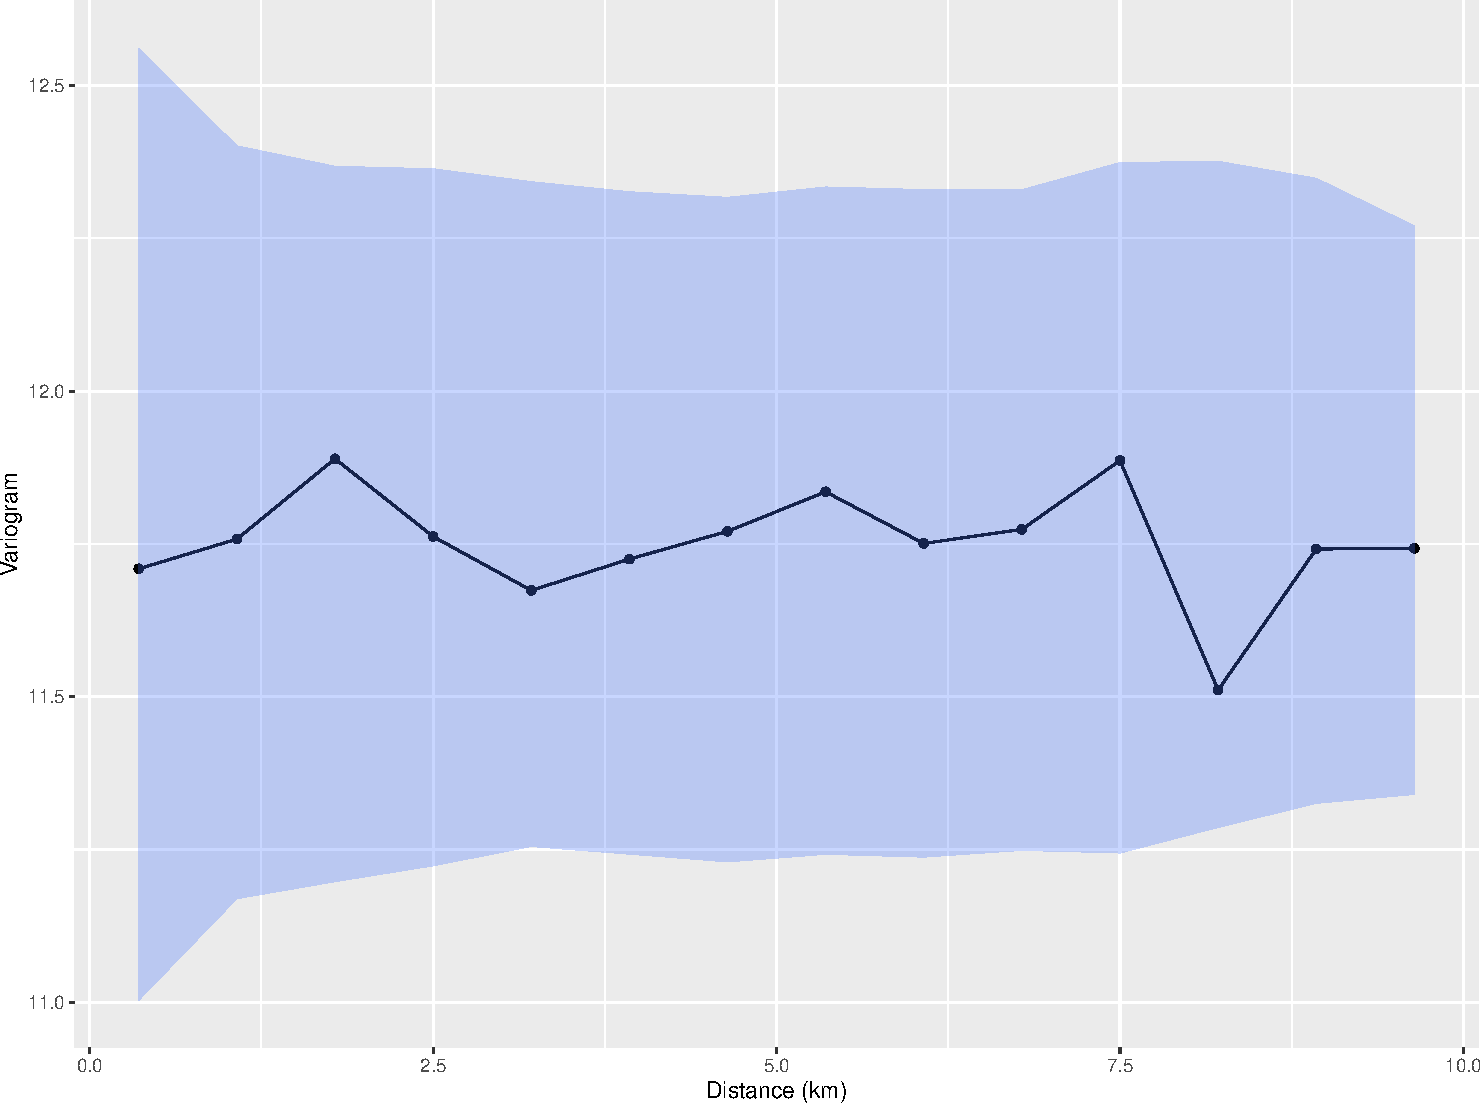
\includegraphics[keepaspectratio]{05_case-studies_files/figure-pdf/fig-wnv-variogram-1.pdf}}

}

\caption{\label{fig-wnv-variogram}Empirical variogram (black line) for
based on the random effects fitted from the model in
Equation~\ref{eq-wnv-counts}. The shaded blue area correspond to the
envelope of spatial independence at 95\% confidence level generated
using a permuation test.}

\end{figure}%

The empirical variogram shown in Figure~\ref{fig-wnv-variogram} lies
entirely within the simulation envelope, indicating no detectable
spatial correlation in the residuals. This lack of evidence may be due
to the fact that mosquito abundance is influenced by very local
environmental conditions such as vegetation, drainage, or breeding site
availability, which vary at spatial scales smaller than 1 km. Since only
a few trap locations in the dataset are spaced closely enough to capture
such fine-scale variation, the analysis may lack the resolution needed
to detect spatial dependence. Therefore, although a geostatistical model
is not justified in this case, we can still pursue our objective of
estimating the average number of mosquitoes at the sampled locations
using the model in Equation~\ref{eq-wnv-counts}.

The principles used in this case to derive the predictive distribution
of \(\lambda(x_i)\), the expected number of mosquitoes at a sampled
location \(x_i\), are similar to those applied in geostatistical models.
However, they take a simplified form here because we do not need to
account for spatial correlation. The predictive distribution is given
by: \begin{equation}\phantomsection\label{eq-pred-distr}{
\left[\lambda(x_i) \:\middle | \: Y_i = y_i \right] = \int [Z_i] \, [Y_i \mid Z_i] \, dZ_i
}\end{equation} In this expression, \([Z_i]\) denotes the density of a
Gaussian distribution with mean zero and variance \(\sigma^2\), and
\([Y_i \mid Z_i]\) is the likelihood from a Poisson model with mean
\(\lambda(x_i)\). The integral in Equation~\ref{eq-pred-distr} can be
computed numerically in R with relative efficiency. This approach also
allows for direct simulation from the predictive distribution, enabling
us to compute any desired summary statistics.

For this analysis, we use a custom function called
\texttt{simulate\_random\_effects}, which can be copied from
Section~\ref{sec-sim-re} and pasted into an R script, as it is not
included in the \texttt{RiskMap} package. Further details of its
implementation are provided in Section~\ref{sec-sim-re}; here, we focus
solely on the analysis.

Hence, we first simulate 1000 samples from the predictive distribution
of \(Z_i\) and denote those by \(Z_i^{(j)}\), for \(i=1,\ldots,598\),
and \(j=1\ldots,1000\).

\begin{Shaded}
\begin{Highlighting}[]
\NormalTok{n\_samples }\OtherTok{\textless{}{-}} \DecValTok{1000}
\NormalTok{samples\_z }\OtherTok{\textless{}{-}} \FunctionTok{simulate\_random\_effects}\NormalTok{(glmer\_wvn, }\AttributeTok{n\_sim =}\NormalTok{ n\_samples)}
\end{Highlighting}
\end{Shaded}

We then obtain predictive samples for \(\lambda(x_i)\) by applying the
exponential transformation to the linear predictor
\(\hat{\mu}_i + Z_{i}^{(j)}\), where in \(\hat{\mu}_i\) we have plugged
in the maximum likelihood estimates of the regression coefficients.

The predictions shown in Figure~\ref{fig-mosq-predictions} indicate that
the pattern of the mean number of mosquitoes across sampled locations is
broadly comparable across time.

\begin{Shaded}
\begin{Highlighting}[]
\CommentTok{\# Create dataframe}
\NormalTok{mosq\_df }\OtherTok{\textless{}{-}} \FunctionTok{data.frame}\NormalTok{(}
  \AttributeTok{id =} \DecValTok{1}\SpecialCharTok{:}\FunctionTok{nrow}\NormalTok{(abund\_sma),}
  \AttributeTok{mean =}\NormalTok{ mosq\_mean,}
  \AttributeTok{lower =}\NormalTok{ mosq\_lower,}
  \AttributeTok{upper =}\NormalTok{ mosq\_upper}
\NormalTok{)}

\CommentTok{\# Adding trap\_group and year}
\NormalTok{mosq\_df}\SpecialCharTok{$}\NormalTok{trap\_group }\OtherTok{\textless{}{-}}\NormalTok{ abund\_sma}\SpecialCharTok{$}\NormalTok{trap\_group[}\FunctionTok{match}\NormalTok{(mosq\_df}\SpecialCharTok{$}\NormalTok{id, abund\_sma}\SpecialCharTok{$}\NormalTok{loc)]}
\NormalTok{mosq\_df}\SpecialCharTok{$}\NormalTok{year }\OtherTok{\textless{}{-}}\NormalTok{ abund\_sma}\SpecialCharTok{$}\NormalTok{year[}\FunctionTok{match}\NormalTok{(mosq\_df}\SpecialCharTok{$}\NormalTok{id, abund\_sma}\SpecialCharTok{$}\NormalTok{loc)]}

\CommentTok{\# Rearranging the data{-}frame in increasing order based}
\CommentTok{\# on the mean number of mosquitoes}
\CommentTok{\# by year and trap group}

\NormalTok{mosq\_df }\OtherTok{\textless{}{-}}\NormalTok{ mosq\_df }\SpecialCharTok{\%\textgreater{}\%}
  \FunctionTok{group\_by}\NormalTok{(year, trap\_group) }\SpecialCharTok{\%\textgreater{}\%}
  \FunctionTok{arrange}\NormalTok{(mean, }\AttributeTok{.by\_group =} \ConstantTok{TRUE}\NormalTok{) }\SpecialCharTok{\%\textgreater{}\%}
  \FunctionTok{mutate}\NormalTok{(}\AttributeTok{x\_order =} \FunctionTok{row\_number}\NormalTok{()) }\SpecialCharTok{\%\textgreater{}\%}
  \FunctionTok{ungroup}\NormalTok{()}

\FunctionTok{library}\NormalTok{(scales)  }\CommentTok{\# Used for reporting the y{-}axis on the log{-}scale}

\FunctionTok{ggplot}\NormalTok{(mosq\_df, }\FunctionTok{aes}\NormalTok{(}\AttributeTok{x =}\NormalTok{ x\_order, }\AttributeTok{y =}\NormalTok{ mean,}
                    \AttributeTok{color =}\NormalTok{ trap\_group, }\AttributeTok{fill =}\NormalTok{ trap\_group, }\AttributeTok{group =}\NormalTok{ trap\_group)) }\SpecialCharTok{+}
  \FunctionTok{geom\_ribbon}\NormalTok{(}\FunctionTok{aes}\NormalTok{(}\AttributeTok{ymin =}\NormalTok{ lower, }\AttributeTok{ymax =}\NormalTok{ upper), }\AttributeTok{alpha =} \FloatTok{0.20}\NormalTok{, }\AttributeTok{linewidth =} \DecValTok{0}\NormalTok{) }\SpecialCharTok{+}
  \FunctionTok{geom\_line}\NormalTok{(}\AttributeTok{linewidth =} \FloatTok{0.9}\NormalTok{) }\SpecialCharTok{+}
  \FunctionTok{scale\_y\_log10}\NormalTok{(}
    \AttributeTok{breaks =} \FunctionTok{c}\NormalTok{(}\DecValTok{1}\NormalTok{, }\DecValTok{10}\NormalTok{, }\DecValTok{100}\NormalTok{, }\DecValTok{1000}\NormalTok{),}
    \AttributeTok{labels =} \FunctionTok{label\_number}\NormalTok{()}
\NormalTok{  ) }\SpecialCharTok{+}
  \FunctionTok{facet\_wrap}\NormalTok{(}\SpecialCharTok{\textasciitilde{}}\NormalTok{year, }\AttributeTok{scales =} \StringTok{"free\_x"}\NormalTok{) }\SpecialCharTok{+}
  \FunctionTok{labs}\NormalTok{(}\AttributeTok{x =} \StringTok{"Locations (ordered within trap group)"}\NormalTok{,}
       \AttributeTok{y =} \StringTok{"Predicted no. mosquitoes (per trap{-}night)"}\NormalTok{,}
       \AttributeTok{color =} \StringTok{"Trap group"}\NormalTok{, }\AttributeTok{fill =} \StringTok{"Trap group"}\NormalTok{) }\SpecialCharTok{+}
  \FunctionTok{theme\_minimal}\NormalTok{()}
\end{Highlighting}
\end{Shaded}

\begin{figure}[H]

\centering{

\pandocbounded{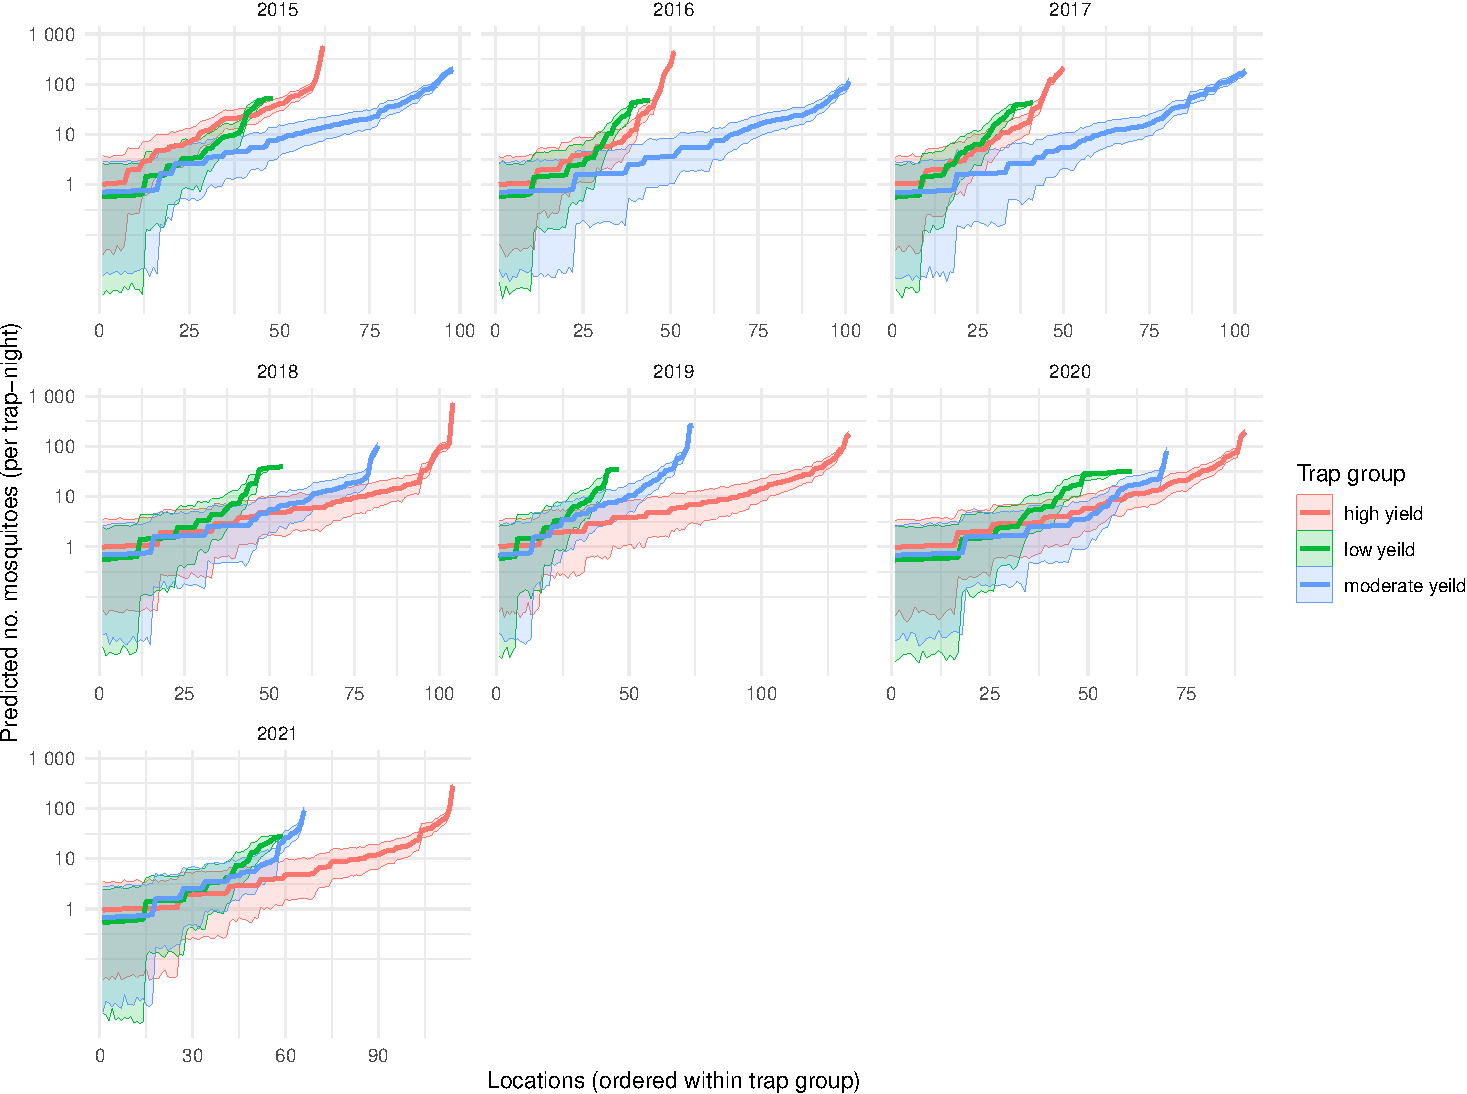
\includegraphics[keepaspectratio]{05_case-studies_files/figure-pdf/fig-mosq-predictions-1.pdf}}

}

\caption{\label{fig-mosq-predictions}Predictive mean number of
mosquitoes per trap-night for each location with 95\% prediction
intervals, stratified by year and trap group. Within each panel,
locations are ordered by increasing predicted mean abundance. Shaded
areas represent 95\% prediction intervals for the number of mosquitoes
at sampled locations. The y-axis is on a log scale, with tick labels
shown on the original scale.}

\end{figure}%

To understand whether we can trust the inferences shown in
Figure~\ref{fig-mosq-predictions}, we use the AnPIT graphical check as
used in the previous case studies. Since we are not using a
geostatistical model in this case, we will use a simplified
implementation of the AnPIT for the Poisson mixed model fitted in this
section. The function that we use to compute the AnPIT is called
\texttt{anpit\_wnv} and has been implemented specifically for this case
study. For more details on its implementation, read
Section~\ref{sec-nonspat-anpit}.

\begin{Shaded}
\begin{Highlighting}[]
\NormalTok{wnv\_anpit\_res }\OtherTok{\textless{}{-}} \FunctionTok{anpit\_wnv}\NormalTok{(glmer\_wvn, }\AttributeTok{test\_prop =} \FloatTok{0.30}\NormalTok{, }\AttributeTok{nsim =} \DecValTok{10000}\NormalTok{)}
\end{Highlighting}
\end{Shaded}

In the code above the AnPIT is computed using a test-set corresponding
to \(30\%\) of the original data-set. The number of simulation used to
approximate the AnPIT is set to 1000. Finally, we plot the results.

\begin{Shaded}
\begin{Highlighting}[]
\FunctionTok{plot\_anpit}\NormalTok{(wnv\_anpit\_res)}
\end{Highlighting}
\end{Shaded}

\begin{figure}[H]

\centering{

\pandocbounded{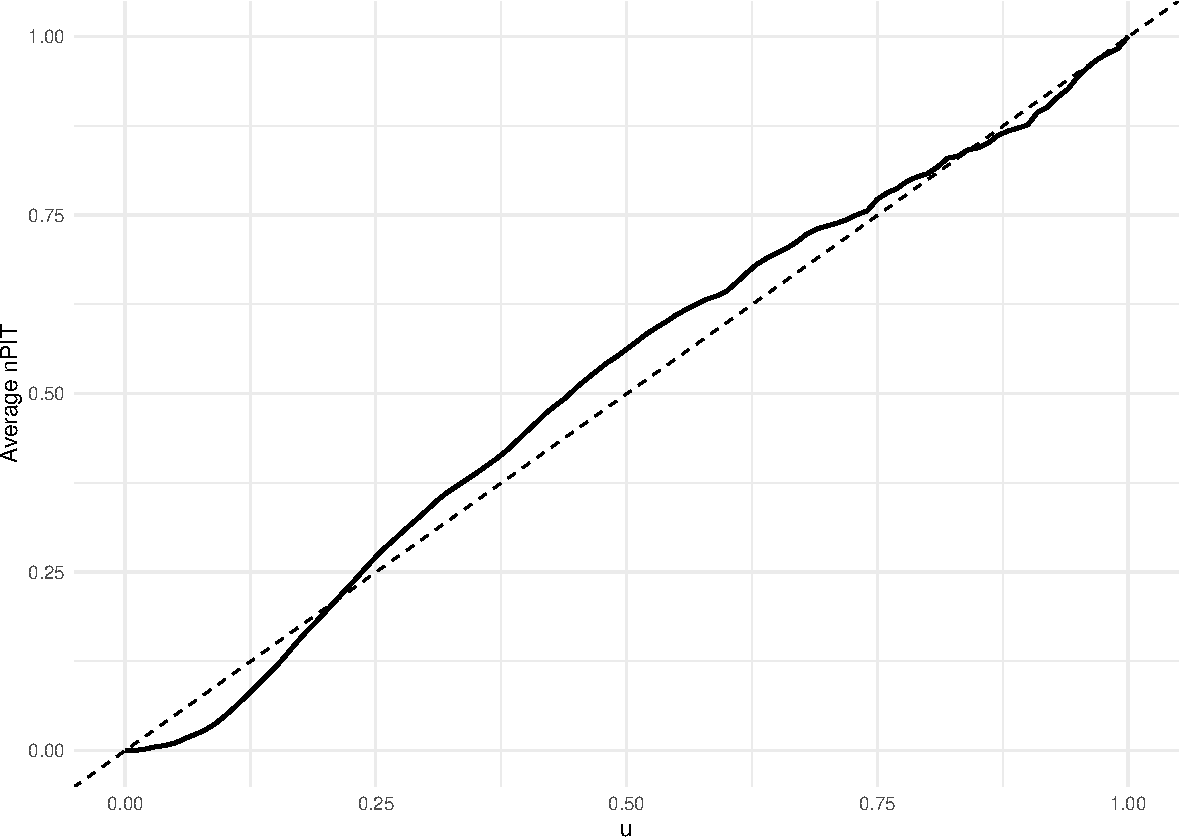
\includegraphics[keepaspectratio]{05_case-studies_files/figure-pdf/fig-wnv-anpit-1.pdf}}

}

\caption{\label{fig-wnv-anpit}Average non-randomized probability
integral transform (AnPIT) for the Poisson mixed model specified in
Equation~\ref{eq-wnv-counts}. The dahsed line corresponds to the
identity line.}

\end{figure}%

The results shown in Figure~\ref{fig-wnv-anpit} an AnPIT curve from the
fitted Poisson mixed model in Figure~\ref{fig-wnv-anpit} that closely
follows the identity line. Hence, we can conclude that we find no
evidence against the compatibility of the model in
Figure~\ref{fig-wnv-anpit} with the data.

\subsection{Modelling West Nile virus infection with pooled mosquito
testing}\label{sec-wnv-model}

Pooled testing is widely used in mosquito surveillance. Rather than
testing each mosquito individually for a pathogen, multiple mosquitoes
collected from the same location and week are combined into a single
pool and assayed by PCR. The test returns positive if at least one
mosquito in the pool is infected and negative otherwise. This approach
greatly reduces laboratory time and costs, but statistical analysis must
account for variation in pool size, as larger pools have a higher
probability of testing positive even if the underlying infection risk
per mosquito is low.

We illustrate this using West Nile virus (WNV) PCR results from pools of
female \emph{Culex pipiens} collected in the Sacramento Metropolitan
Area, available in the \texttt{infect\_sma} data set of the
\texttt{RiskMap} package.

Let \(k_i\) be the number of mosquitoes in pool \(i\). Define the binary
outcome \(Y_i=1\) if the PCR test for pool \(i\) is positive and
\(Y_i=0\) otherwise. Conditional on a stationary and isotropic spatial
Gaussian process \(S(x_i)\), the probability that pool \(i\) is positive
is\\
\begin{equation}\phantomsection\label{eq-wnv-pos-model}{
P(Y_i=1\mid S(x_i))=1-\left[1-p(x_i)\right]^{k_i},
}\end{equation} where \(p(x_i)\) is the probability that an individual
mosquito at location \(x_i\) is infected with WNV. We model \(p(x_i)\)
using a logit-linear form\\
\begin{equation}\phantomsection\label{eq-wnv-lp}{
\log\left\{\frac{p(x_i)}{1-p(x_i)}\right\}=\beta+S(x_i),
}\end{equation} which explicitly incorporates the dependence of the pool
positivity probability on pool size \(k_i\).

We must emphasize that in the \texttt{infect\_sma} data set the pool
sizes \(k_i\) are not taken directly from laboratory records but are
estimated. For each pool, mosquito collections from nearby locations in
the same epidemiological week and within a given spatial radius, for
example 2 km, are identified. The total number of female mosquitoes from
these nearby collections, denoted \(T_{\text{near}}\), is divided by the
number of pools formed from the same nearby collections in that week,
denoted \(m_{\text{near}}\), to obtain an estimate of pool size. The
estimated pool size is therefore\\
\[
\widehat{k}_i=\text{round}\left(\max\{1,T_{\text{near}}/m_{\text{near}}\}\right),
\] and a default conservative value, such as 25, is used if no nearby
collections are available.

The data comprise 596 responses, of which only 18 pools test positive.
This very low prevalence constrains our modelling choices, for example
by limiting the feasibility of incorporating temporal dynamics. As a
result, the model in Equation~\ref{eq-wnv-pos-model} represents the
simplest specification that can still capture spatial correlation, under
the simplifying assumption that WNV risk remains relatively stable over
the study period. Furthermore, because there is only a single binary
outcome per location, overdispersion cannot occur (see box ``Why
Bernoulli extra‐variation does not exist'' in Section 5.1.1 of P. J.
Diggle and Giorgi (2019)), and the empirical variogram provides limited
value for assessing spatial correlation due to its high uncertainty in
this context. We therefore proceed directly to fitting a geostatistical
model and assess the estimate of the spatial correlation parameter,
which quantifies the strength and range of spatial dependence in the
data.

We then proceed in R as follows. We first load the data and convert them
into an \texttt{sf} object with the appropriate UTM projection.

\begin{Shaded}
\begin{Highlighting}[]
\FunctionTok{data}\NormalTok{(infect\_sma)}

\NormalTok{infect\_sma }\OtherTok{\textless{}{-}} \FunctionTok{st\_as\_sf}\NormalTok{(infect\_sma, }\AttributeTok{coords =} \FunctionTok{c}\NormalTok{(}\StringTok{"lon"}\NormalTok{, }\StringTok{"lat"}\NormalTok{), }\AttributeTok{crs =} \DecValTok{4326}\NormalTok{)}
\NormalTok{wnv\_crs }\OtherTok{\textless{}{-}} \FunctionTok{propose\_utm}\NormalTok{(infect\_sma)}
\NormalTok{infect\_sma }\OtherTok{\textless{}{-}} \FunctionTok{st\_transform}\NormalTok{(infect\_sma, wnv\_crs)}
\end{Highlighting}
\end{Shaded}

We define the inverse link function based on
Equation~\ref{eq-wnv-pos-model} and Equation~\ref{eq-wnv-lp}.

\begin{Shaded}
\begin{Highlighting}[]
\NormalTok{invlink\_wnv }\OtherTok{\textless{}{-}} \ControlFlowTok{function}\NormalTok{(x) }\DecValTok{1}\SpecialCharTok{{-}}\NormalTok{(}\DecValTok{1}\SpecialCharTok{{-}}\FunctionTok{exp}\NormalTok{(x)}\SpecialCharTok{/}\NormalTok{(}\DecValTok{1}\SpecialCharTok{+}\FunctionTok{exp}\NormalTok{(x)))}\SpecialCharTok{\^{}}\NormalTok{infect\_sma}\SpecialCharTok{$}\NormalTok{est\_pool\_n}
\end{Highlighting}
\end{Shaded}

We then fit the model by passing the inverse link function to the
argument \texttt{invlink} within the \texttt{glgpm} function.

\begin{Shaded}
\begin{Highlighting}[]
\NormalTok{inf\_fit }\OtherTok{\textless{}{-}}
  \FunctionTok{glgpm}\NormalTok{(wnv\_pos }\SpecialCharTok{\textasciitilde{}} \FunctionTok{gp}\NormalTok{(lon,lat),}
        \AttributeTok{crs =}\NormalTok{ wnv\_crs,}
        \AttributeTok{family =} \StringTok{"binomial"}\NormalTok{,}
        \AttributeTok{invlink =}\NormalTok{ invlink\_wnv,}
        \AttributeTok{data=}\NormalTok{infect\_sma)}
\end{Highlighting}
\end{Shaded}

Finally, we examine the the summary of the fitted model.

\begin{Shaded}
\begin{Highlighting}[]
\FunctionTok{summary}\NormalTok{(inf\_fit)}
\end{Highlighting}
\end{Shaded}

\begin{verbatim}
Call:
glgpm(formula = wnv_pos ~ gp(lon, lat), data = infect_sma, family = "binomial", 
    invlink = invlink_wnv, crs = wnv_crs, par0 = coef(inf_fit), 
    start_pars = coef(inf_fit))

Binomial geostatistical linear model
Link: custom 
Inverse link function = 1 - (1 - exp(x)/(1 + exp(x)))^infect_sma$est_pool_n 
 
'Lower limit' and 'Upper limit' are the limits of the 95% confidence level intervals

Regression coefficients
            Estimate Lower limit Upper limit  StdErr z.value  p.value    
(Intercept)  -4.9648     -7.0190     -2.9105  1.0481 -4.7369 2.17e-06 ***
---
Signif. codes:  0 '***' 0.001 '**' 0.01 '*' 0.05 '.' 0.1 ' ' 1

Spatial Gaussian process
Matern covariance parameters (kappa=0.5)
                     Estimate Lower limit Upper limit
Spatial process var.   5.9851      1.5402      23.259
Spatial corr. scale   24.5370      9.1354      65.905
Variance of the nugget effect fixed at 0

Log-likelihood: 0.4061681
\end{verbatim}

The fitted model indicates a substantial spatial residual component,
with the estimated scale parameter corresponding to a practical range of
approximately 70 km. This represents a long‐range correlation relative
to the spatial extent of the study area.

We first carry out predictions over a regular grid covering the area of
the data collection efforts from 2015 to 2021. To achieve this, we
create a regular grid 250 meters within the convex hull boundaries
obtained by the full set of locations sampled from 2015 to 2021 (see
Figure~\ref{fig-wnv-convex-hull}).

\begin{Shaded}
\begin{Highlighting}[]
\CommentTok{\# Compute convex hull}
\NormalTok{geom\_union }\OtherTok{\textless{}{-}} \FunctionTok{st\_union}\NormalTok{(inf\_fit}\SpecialCharTok{$}\NormalTok{data\_sf)}
\NormalTok{chull\_sf }\OtherTok{\textless{}{-}} \FunctionTok{st\_convex\_hull}\NormalTok{(geom\_union)}
\NormalTok{chull\_sf }\OtherTok{\textless{}{-}} \FunctionTok{st\_as\_sf}\NormalTok{(}\FunctionTok{data.frame}\NormalTok{(}\AttributeTok{geometry =} \FunctionTok{st\_sfc}\NormalTok{(chull\_sf)),}
                     \AttributeTok{crs =} \FunctionTok{st\_crs}\NormalTok{(inf\_fit}\SpecialCharTok{$}\NormalTok{data\_sf))}

\CommentTok{\# Plot points and convex hull}
\FunctionTok{ggplot}\NormalTok{() }\SpecialCharTok{+}
  \FunctionTok{geom\_sf}\NormalTok{(}\AttributeTok{data =}\NormalTok{ inf\_fit}\SpecialCharTok{$}\NormalTok{data\_sf, }\AttributeTok{color =} \StringTok{"blue"}\NormalTok{, }\AttributeTok{size =} \DecValTok{1}\NormalTok{) }\SpecialCharTok{+}
  \FunctionTok{geom\_sf}\NormalTok{(}\AttributeTok{data =}\NormalTok{ chull\_sf, }\AttributeTok{fill =} \ConstantTok{NA}\NormalTok{, }\AttributeTok{color =} \StringTok{"red"}\NormalTok{, }\AttributeTok{linewidth =} \DecValTok{1}\NormalTok{) }\SpecialCharTok{+}
  \FunctionTok{theme\_minimal}\NormalTok{()}
\end{Highlighting}
\end{Shaded}

\begin{figure}[H]

\centering{

\pandocbounded{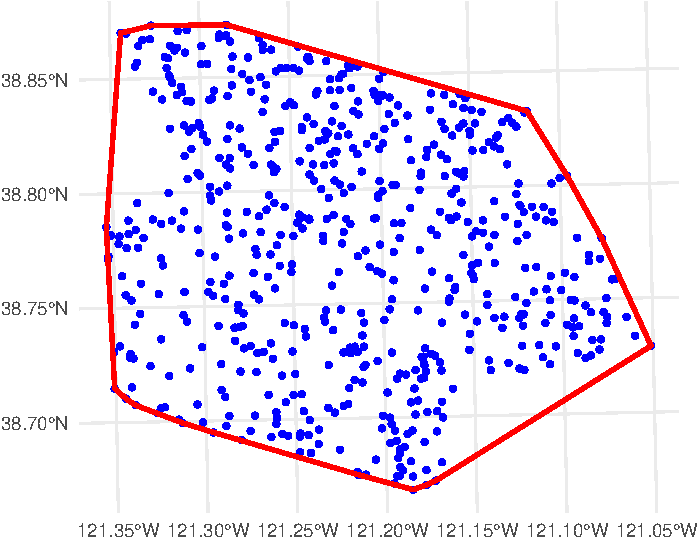
\includegraphics[keepaspectratio]{05_case-studies_files/figure-pdf/fig-wnv-convex-hull-1.pdf}}

}

\caption{\label{fig-wnv-convex-hull}Sampling locations of pooled
mosquito collections testing for West Nile virus in the Sacramento
Metropolitan Area (blue points) and their convex hull (red outline)
defining the minimal polygon enclosing all sites.}

\end{figure}%

\begin{Shaded}
\begin{Highlighting}[]
\NormalTok{grid\_pred\_sac }\OtherTok{\textless{}{-}} \FunctionTok{create\_grid}\NormalTok{(chull\_sf, }\AttributeTok{spat\_res =} \FloatTok{0.25}\NormalTok{)}

\NormalTok{pred\_S\_inf }\OtherTok{\textless{}{-}} \FunctionTok{pred\_over\_grid}\NormalTok{(inf\_fit,}
                             \AttributeTok{grid\_pred =}\NormalTok{ grid\_pred\_sac)}

\NormalTok{pred\_inf\_grid }\OtherTok{\textless{}{-}} \FunctionTok{pred\_target\_grid}\NormalTok{(pred\_S\_inf,}
                                  \AttributeTok{f\_target =} \FunctionTok{list}\NormalTok{(}\AttributeTok{prev =} \ControlFlowTok{function}\NormalTok{(x) }\FunctionTok{exp}\NormalTok{(x)}\SpecialCharTok{/}\NormalTok{(}\DecValTok{1}\SpecialCharTok{+}\FunctionTok{exp}\NormalTok{(x))))}
\end{Highlighting}
\end{Shaded}

Figure~\ref{fig-wnv-pred-map} displays the predictive mean of \(p(x)\)
over the regular grid. Overall, the predicted prevalence of WNV is very
low across the study area, with a small zone in the south‐west showing a
relatively higher value of approximately \(0.40\%\).

\begin{Shaded}
\begin{Highlighting}[]
\FunctionTok{plot}\NormalTok{(pred\_inf\_grid,}\StringTok{"prev"}\NormalTok{)}
\end{Highlighting}
\end{Shaded}

\begin{figure}[H]

\centering{

\pandocbounded{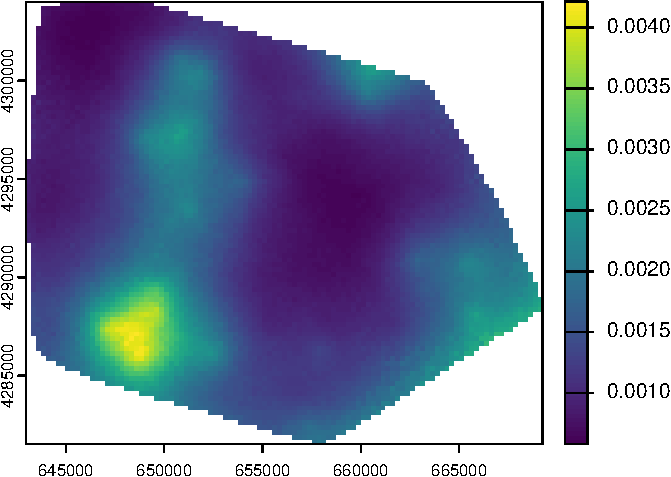
\includegraphics[keepaspectratio]{05_case-studies_files/figure-pdf/fig-wnv-pred-map-1.pdf}}

}

\caption{\label{fig-wnv-pred-map}Map of the predictive mean for the
prevalence of West Nile Virus infection among female \emph{Culex
pipiens} mosquitoes in an area of the Sacramento Metropolitan Area.}

\end{figure}%

Finally, we predict the vector index as defined in Equation~\ref{eq-vi}.
Because \emph{Cx. pipiens} abundance and WNV infection prevalence have
been modelled as independent processes, the predictions from the two
models can be combined directly. Specifically, for each location in the
\texttt{abund\_sma} data set, we take predictive samples of WNV
prevalence and multiply them by the corresponding predictive samples of
the mean number of female \emph{Cx. pipiens} per trap‐night. This yields
predictive samples of the vector index, which can then be summarised or
mapped as required. In R, this is implemented as follows.

\begin{Shaded}
\begin{Highlighting}[]
\CommentTok{\# Converting the abund\_sma into an sf object}
\NormalTok{loc\_pred }\OtherTok{\textless{}{-}} \FunctionTok{st\_as\_sfc}\NormalTok{(}\FunctionTok{st\_transform}\NormalTok{(}\FunctionTok{st\_as\_sf}\NormalTok{(abund\_sma, }\AttributeTok{coords =} \FunctionTok{c}\NormalTok{(}\StringTok{"lon"}\NormalTok{,}\StringTok{"lat"}\NormalTok{), }\AttributeTok{crs =} \DecValTok{4326}\NormalTok{), }\AttributeTok{crs =}\NormalTok{ wnv\_crs))}

\CommentTok{\# Prediction of the sptial process S(x) over the locations of the }
\CommentTok{\# abund\_sma data{-}set}
\NormalTok{pred\_S\_loc }\OtherTok{\textless{}{-}} \FunctionTok{pred\_over\_grid}\NormalTok{(inf\_fit, }\AttributeTok{grid\_pred =}\NormalTok{ loc\_pred)}

\CommentTok{\# Computation of the samples for West Nile Virus prevalence}
\NormalTok{beta\_hat }\OtherTok{\textless{}{-}} \FunctionTok{coef}\NormalTok{(inf\_fit)}\SpecialCharTok{$}\NormalTok{beta}
\NormalTok{prev\_inf\_samples }\OtherTok{\textless{}{-}} \DecValTok{1}\SpecialCharTok{/}\NormalTok{(}\DecValTok{1}\SpecialCharTok{+}\FunctionTok{exp}\NormalTok{(}\SpecialCharTok{{-}}\NormalTok{(beta\_hat }\SpecialCharTok{+}
\NormalTok{                                 pred\_S\_loc}\SpecialCharTok{$}\NormalTok{S\_samples)))}

\CommentTok{\# Predictive samples for the vector index (VI)}
\NormalTok{vi\_samples }\OtherTok{\textless{}{-}}\NormalTok{ mean\_nmosq }\SpecialCharTok{*}\NormalTok{ prev\_inf\_samples}

\CommentTok{\# Calculate predictive summaries for VI}
\NormalTok{vi\_mean  }\OtherTok{\textless{}{-}} \FunctionTok{apply}\NormalTok{(vi\_samples, }\DecValTok{1}\NormalTok{, mean, }\AttributeTok{na.rm =} \ConstantTok{TRUE}\NormalTok{)}
\NormalTok{vi\_lower }\OtherTok{\textless{}{-}} \FunctionTok{apply}\NormalTok{(vi\_samples, }\DecValTok{1}\NormalTok{, quantile, }\AttributeTok{probs =} \FloatTok{0.025}\NormalTok{, }\AttributeTok{na.rm =} \ConstantTok{TRUE}\NormalTok{)}
\NormalTok{vi\_upper }\OtherTok{\textless{}{-}} \FunctionTok{apply}\NormalTok{(vi\_samples, }\DecValTok{1}\NormalTok{, quantile, }\AttributeTok{probs =} \FloatTok{0.975}\NormalTok{, }\AttributeTok{na.rm =} \ConstantTok{TRUE}\NormalTok{)}

\CommentTok{\# Build dataframe directly from original abund\_sma order}
\NormalTok{vi\_df }\OtherTok{\textless{}{-}} \FunctionTok{data.frame}\NormalTok{(}
  \AttributeTok{id    =} \DecValTok{1}\SpecialCharTok{:}\FunctionTok{nrow}\NormalTok{(abund\_sma),}
  \AttributeTok{mean  =}\NormalTok{ vi\_mean,}
  \AttributeTok{lower =}\NormalTok{ vi\_lower,}
  \AttributeTok{upper =}\NormalTok{ vi\_upper,}
  \AttributeTok{trap\_group =}\NormalTok{ abund\_sma}\SpecialCharTok{$}\NormalTok{trap\_group,}
  \AttributeTok{year       =}\NormalTok{ abund\_sma}\SpecialCharTok{$}\NormalTok{year}
\NormalTok{)}

\CommentTok{\# Order within (year, trap\_group) by increasing mean}
\NormalTok{vi\_df }\OtherTok{\textless{}{-}}\NormalTok{ vi\_df }\SpecialCharTok{\%\textgreater{}\%}
  \FunctionTok{group\_by}\NormalTok{(year, trap\_group) }\SpecialCharTok{\%\textgreater{}\%}
  \FunctionTok{arrange}\NormalTok{(mean, }\AttributeTok{.by\_group =} \ConstantTok{TRUE}\NormalTok{) }\SpecialCharTok{\%\textgreater{}\%}
  \FunctionTok{mutate}\NormalTok{(}\AttributeTok{x\_order =}\NormalTok{ dplyr}\SpecialCharTok{::}\FunctionTok{row\_number}\NormalTok{()) }\SpecialCharTok{\%\textgreater{}\%}
  \FunctionTok{ungroup}\NormalTok{()}
\end{Highlighting}
\end{Shaded}

Several U.S. programs consider a vector index (VI) of 0.75 or higher as
indicative of likely human transmission and use this threshold to
trigger intensified control measures (City of Boulder 2025; City of Fort
Collins 2025, 2014). In Figure~\ref{fig-vi}, the dashed red line marks
this operational threshold for elevated WNV risk. We observe that only
in few instances before the year 2020 the predicted VI exceeded this
threshold. We thus conclude that between 2015 and 2021 the risk for WNV
based as measured by the VI was relatively low in the SMA.

\begin{Shaded}
\begin{Highlighting}[]
\FunctionTok{ggplot}\NormalTok{(vi\_df,}
       \FunctionTok{aes}\NormalTok{(}\AttributeTok{x =}\NormalTok{ x\_order, }\AttributeTok{y =}\NormalTok{ mean,}
           \AttributeTok{color =}\NormalTok{ trap\_group, }\AttributeTok{fill =}\NormalTok{ trap\_group, }\AttributeTok{group =}\NormalTok{ trap\_group)) }\SpecialCharTok{+}
  \FunctionTok{geom\_hline}\NormalTok{(}\AttributeTok{yintercept =} \FloatTok{0.75}\NormalTok{, }\AttributeTok{linetype =} \StringTok{"dashed"}\NormalTok{, }\AttributeTok{color =} \StringTok{"red"}\NormalTok{, }\AttributeTok{linewidth =} \FloatTok{0.8}\NormalTok{) }\SpecialCharTok{+}
  \FunctionTok{geom\_ribbon}\NormalTok{(}\FunctionTok{aes}\NormalTok{(}\AttributeTok{ymin =}\NormalTok{ lower, }\AttributeTok{ymax =}\NormalTok{ upper), }\AttributeTok{alpha =} \FloatTok{0.20}\NormalTok{, }\AttributeTok{linewidth =} \DecValTok{0}\NormalTok{) }\SpecialCharTok{+}
  \FunctionTok{geom\_line}\NormalTok{(}\AttributeTok{linewidth =} \FloatTok{0.9}\NormalTok{) }\SpecialCharTok{+}
  \FunctionTok{scale\_y\_log10}\NormalTok{(}
    \AttributeTok{breaks =} \FunctionTok{c}\NormalTok{(}\FloatTok{0.01}\NormalTok{, }\FloatTok{0.1}\NormalTok{, }\DecValTok{1}\NormalTok{),}
    \AttributeTok{labels =}\NormalTok{ scales}\SpecialCharTok{::}\FunctionTok{label\_number}\NormalTok{()}
\NormalTok{  ) }\SpecialCharTok{+}
  \FunctionTok{facet\_wrap}\NormalTok{(}\SpecialCharTok{\textasciitilde{}}\NormalTok{ year, }\AttributeTok{scales =} \StringTok{"free\_x"}\NormalTok{) }\SpecialCharTok{+}
  \FunctionTok{labs}\NormalTok{(}
    \AttributeTok{x =} \StringTok{"Locations (ordered within trap group)"}\NormalTok{,}
    \AttributeTok{y =} \StringTok{"Vector index (infected mosquitoes per trap night)"}\NormalTok{,}
    \AttributeTok{title =} \StringTok{"West Nile Virus"}\NormalTok{,}
    \AttributeTok{color =} \StringTok{"Trap group"}\NormalTok{, }\AttributeTok{fill =} \StringTok{"Trap group"}
\NormalTok{  ) }\SpecialCharTok{+}
  \FunctionTok{theme\_minimal}\NormalTok{()}
\end{Highlighting}
\end{Shaded}

\begin{figure}[H]

\centering{

\pandocbounded{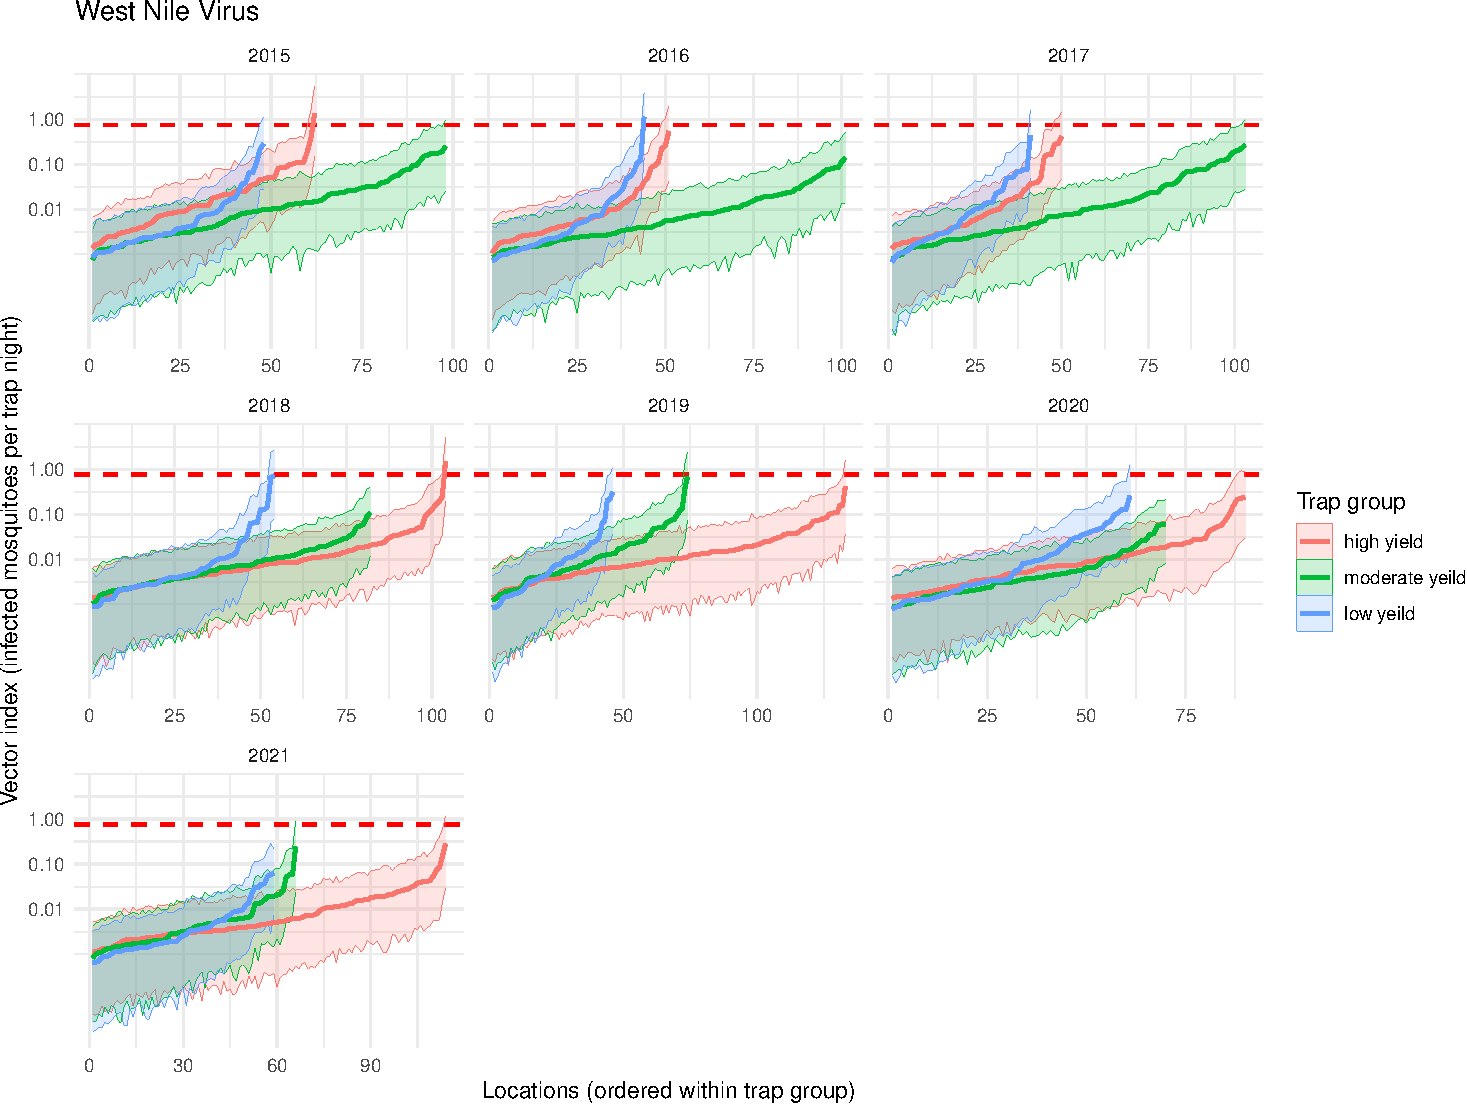
\includegraphics[keepaspectratio]{05_case-studies_files/figure-pdf/fig-vi-1.pdf}}

}

\caption{\label{fig-vi}Predicted vector index (infected mosquitoes per
trap night) by location, stratified by year and trap group. Locations
within each panel are ordered by increasing predicted VI. Shaded bands
represent 95\% prediction intervals. The dashed red line marks the 0.75
threshold commonly used in U.S. West Nile virus surveillance to indicate
elevated transmission risk. The y-axis is on a log scale with labels
shown on the original scale.}

\end{figure}%

\subsection{Summary and conclusions}\label{sec-summary-wnv}

In this analysis, our predictive target was the vector index (VI) in
Equation~\ref{eq-vi}. Our proposed modelling approach was based on the
assumption that abundance and infection prevalence are two independent
processes. Treating prevalence as independent of vector density is a
practical simplification. It can be reasonable when the fraction of
infected mosquitoes at a place and time is driven mainly by host
infection dynamics, temperature dependent incubation, and mosquito age
structure, whereas trap counts reflect local production, as well as
catchability. An interesting result of our analysis is that abundance
showed no detectable residual spatial correlation, while infection
prevalence did. The empirical variogram of random effects from the
abundance model lay within the envelope in
Figure~\ref{fig-wnv-variogram}, suggesting that remaining variation
after accounting for year and trap group is dominated by micro scale
heterogeneity and trap specific noise at distances smaller than those
represented by the sampling design. In contrast, the infection model
estimated a spatial scale of correlation that is large relative to the
study area, and may be explained in terms of processes that operate over
broader extents, such as movement and aggregation of avian reservoir
hosts, shared urban landscape features, and temperature fields. However,
as a result of the disparity in the scales of spatial dependence for the
two processes and the inability of the model for abundance to
interpolate at unobserved locations, we could only predict the VI at the
observed locations of the abundance data.

All West Nile virus data analysed in this section originate from the
\texttt{vectorsurvR} workflow and are simulated rather than observed in
the field. The \texttt{vectorsurvR} package provides a framework for
generating realistic mosquito surveillance data by mimicking the
structure, spatial layout, and sampling frequency of actual surveillance
programmes. Hence, the results presented here should not be used to draw
scientific conclusions about West Nile virus in the Sacramento
Metropolitan Area. In addition to this, pool size is a key input when
analysing pooled infection outcomes (see Exercise 6 below) and strongly
affects the predictive inferences in prevalence (see Exercise 6 below).
In this case study we used an estimated pool size (denoted in the text
above by \(k_i\)) rather than laboratory recorded counts, which adds
additional uncertainty that we did not propagate. The results illustrate
modelling steps, diagnostics, and how to combine components to obtain
the vector index, which remains useful for pedagogical purposes.

\section{Theory}\label{theory-1}

In the following two sections we explain the coding of the functions
used in Section~\ref{sec-abund-model}. These functions are not part of
any existing R package. They are written for clarity rather than
computational efficiency, and they are tailored to the current modelling
example without attempts at generalisation. The aim is to present code
that is correct and easy to follow, so that by understanding each
component you can adapt and extend it to fit your own modelling
requirements and learn more efficient implementations your own.

\subsection{Simulating from the predictive of non-spatial mixed
models}\label{sec-sim-re}

In this section, we provide a detailed explanation of the
simulate\_random\_effects function used in this case study.

Simulating from the conditional distribution of \(Z_i\)\hspace{0pt}
given the observed counts \(y_i\)\hspace{0pt} under a Poisson mixed
model can be done in several ways in R, often more efficiently than the
approach illustrated here. However, our goal is not to present the
fastest implementation, but to offer a transparent, step-by-step
example. This level of detail is useful for readers who wish to
understand the underlying computations, or who may want to adapt and
generalize the function for other analyses. From a pedagogical
perspective, dissecting such a function provides a hands-on introduction
to computational methods for generalized linear mixed models and
illustrates ideas that are extended in more advanced Bayesian and
likelihood-based approaches.

The function is reproduced below:

\begin{Shaded}
\begin{Highlighting}[]
\NormalTok{simulate\_random\_effects }\OtherTok{\textless{}{-}} \ControlFlowTok{function}\NormalTok{(model, }\AttributeTok{nsim =} \DecValTok{1000}\NormalTok{, }\AttributeTok{grid\_range =} \FunctionTok{c}\NormalTok{(}\SpecialCharTok{{-}}\DecValTok{10}\NormalTok{, }\DecValTok{10}\NormalTok{), }\AttributeTok{grid\_length =} \DecValTok{5000}\NormalTok{) \{}
  \CommentTok{\# Extract fixed effects and RE variance}
\NormalTok{  beta\_hat }\OtherTok{\textless{}{-}} \FunctionTok{fixef}\NormalTok{(model)}
\NormalTok{  sigma2\_hat }\OtherTok{\textless{}{-}} \FunctionTok{as.numeric}\NormalTok{(}\FunctionTok{VarCorr}\NormalTok{(model)[[}\DecValTok{1}\NormalTok{]][}\DecValTok{1}\NormalTok{])}
  
  \CommentTok{\# Extract model frame and grouping}
\NormalTok{  mf }\OtherTok{\textless{}{-}}\NormalTok{ model}\SpecialCharTok{@}\NormalTok{frame}
\NormalTok{  group\_var }\OtherTok{\textless{}{-}} \FunctionTok{names}\NormalTok{(}\FunctionTok{ranef}\NormalTok{(model))[}\DecValTok{1}\NormalTok{]}
\NormalTok{  group\_ids }\OtherTok{\textless{}{-}}\NormalTok{ mf[[group\_var]]}
\NormalTok{  unique\_groups }\OtherTok{\textless{}{-}} \FunctionTok{unique}\NormalTok{(group\_ids)}
\NormalTok{  ngroups }\OtherTok{\textless{}{-}} \FunctionTok{length}\NormalTok{(unique\_groups)}
  
  \CommentTok{\# Design matrix for fixed effects}
\NormalTok{  D }\OtherTok{\textless{}{-}} \FunctionTok{model.matrix}\NormalTok{(model)}
  
  \CommentTok{\# Create result matrix}
\NormalTok{  u\_samples }\OtherTok{\textless{}{-}} \FunctionTok{matrix}\NormalTok{(}\ConstantTok{NA}\NormalTok{, }\AttributeTok{nrow =}\NormalTok{ ngroups, }\AttributeTok{ncol =}\NormalTok{ nsim)}
  \FunctionTok{rownames}\NormalTok{(u\_samples) }\OtherTok{\textless{}{-}}\NormalTok{ unique\_groups}
  
  \CommentTok{\# Log{-}predictive density function for one group}
\NormalTok{  log\_pd\_u }\OtherTok{\textless{}{-}} \ControlFlowTok{function}\NormalTok{(u, y\_j, D\_j, beta\_hat, sigma2\_hat) \{}
\NormalTok{    eta }\OtherTok{\textless{}{-}} \FunctionTok{as.vector}\NormalTok{(D\_j }\SpecialCharTok{\%*\%}\NormalTok{ beta\_hat) }\SpecialCharTok{+}\NormalTok{ u}
\NormalTok{    loglik }\OtherTok{\textless{}{-}} \FunctionTok{sum}\NormalTok{(}\FunctionTok{dpois}\NormalTok{(y\_j, }\AttributeTok{lambda =} \FunctionTok{exp}\NormalTok{(eta), }\AttributeTok{log =} \ConstantTok{TRUE}\NormalTok{))}
\NormalTok{    logprior }\OtherTok{\textless{}{-}} \FunctionTok{dnorm}\NormalTok{(u, }\AttributeTok{mean =} \DecValTok{0}\NormalTok{, }\AttributeTok{sd =} \FunctionTok{sqrt}\NormalTok{(sigma2\_hat), }\AttributeTok{log =} \ConstantTok{TRUE}\NormalTok{)}
    \FunctionTok{return}\NormalTok{(loglik }\SpecialCharTok{+}\NormalTok{ logprior)}
\NormalTok{  \}}
  
  \CommentTok{\# For each group, compute predictive samples of u\_j}
  \ControlFlowTok{for}\NormalTok{ (j }\ControlFlowTok{in} \FunctionTok{seq\_along}\NormalTok{(unique\_groups)) \{}
\NormalTok{    gid }\OtherTok{\textless{}{-}}\NormalTok{ unique\_groups[j]}
\NormalTok{    idx }\OtherTok{\textless{}{-}} \FunctionTok{which}\NormalTok{(group\_ids }\SpecialCharTok{==}\NormalTok{ gid)}
\NormalTok{    y\_j }\OtherTok{\textless{}{-}}\NormalTok{ model}\SpecialCharTok{@}\NormalTok{resp}\SpecialCharTok{$}\NormalTok{y[idx]}
\NormalTok{    D\_j }\OtherTok{\textless{}{-}}\NormalTok{ D[idx, , drop }\OtherTok{=} \ConstantTok{FALSE}\NormalTok{]}
    
    \CommentTok{\# Create grid and compute log predictive density}
\NormalTok{    u\_grid }\OtherTok{\textless{}{-}} \FunctionTok{seq}\NormalTok{(grid\_range[}\DecValTok{1}\NormalTok{], grid\_range[}\DecValTok{2}\NormalTok{], }\AttributeTok{length.out =}\NormalTok{ grid\_length)}
\NormalTok{    logdens }\OtherTok{\textless{}{-}} \FunctionTok{sapply}\NormalTok{(u\_grid, log\_pd\_u, }\AttributeTok{y\_j =}\NormalTok{ y\_j, }\AttributeTok{D\_j =}\NormalTok{ D\_j,}
                      \AttributeTok{beta\_hat =}\NormalTok{ beta\_hat, }\AttributeTok{sigma2\_hat =}\NormalTok{ sigma2\_hat)}
\NormalTok{    logdens }\OtherTok{\textless{}{-}}\NormalTok{ logdens }\SpecialCharTok{{-}} \FunctionTok{max}\NormalTok{(logdens)}
\NormalTok{    dens }\OtherTok{\textless{}{-}} \FunctionTok{exp}\NormalTok{(logdens)}
\NormalTok{    pdf\_u }\OtherTok{\textless{}{-}}\NormalTok{ dens }\SpecialCharTok{/} \FunctionTok{sum}\NormalTok{(dens)}
\NormalTok{    cdf\_u }\OtherTok{\textless{}{-}} \FunctionTok{cumsum}\NormalTok{(pdf\_u)}
\NormalTok{    cdf\_u }\OtherTok{\textless{}{-}}\NormalTok{ cdf\_u }\SpecialCharTok{/} \FunctionTok{max}\NormalTok{(cdf\_u)}
    
    \CommentTok{\# Drop duplicated CDF values (necessary for approx)}
\NormalTok{    keep }\OtherTok{\textless{}{-}} \SpecialCharTok{!}\FunctionTok{duplicated}\NormalTok{(cdf\_u)}
\NormalTok{    u\_samples[j, ] }\OtherTok{\textless{}{-}} \FunctionTok{approx}\NormalTok{(cdf\_u[keep], u\_grid[keep], }\AttributeTok{xout =} \FunctionTok{runif}\NormalTok{(nsim), }\AttributeTok{rule =} \DecValTok{2}\NormalTok{)}\SpecialCharTok{$}\NormalTok{y}
    
\NormalTok{  \}}
  
  \FunctionTok{return}\NormalTok{(u\_samples)}
\NormalTok{\}}
\end{Highlighting}
\end{Shaded}

Below, we break down the function step by step.

First, we extract the fixed-effect estimates and the random effect
variance from the fitted model:

\begin{Shaded}
\begin{Highlighting}[]
\NormalTok{beta\_hat }\OtherTok{\textless{}{-}} \FunctionTok{fixef}\NormalTok{(model)                        }\CommentTok{\# Fixed effect coefficients (MLEs)}
\NormalTok{sigma2\_hat }\OtherTok{\textless{}{-}} \FunctionTok{as.numeric}\NormalTok{(}\FunctionTok{VarCorr}\NormalTok{(model)[[}\DecValTok{1}\NormalTok{]][}\DecValTok{1}\NormalTok{])}\CommentTok{\# Estimated variance of random intercepts}
\end{Highlighting}
\end{Shaded}

These parameters will be treated as known when simulating the predictive
of the random effects. Next, we identify the grouping variable for the
random effects and compute the fixed-effects design matrix:

\begin{Shaded}
\begin{Highlighting}[]
\NormalTok{mf }\OtherTok{\textless{}{-}}\NormalTok{ model}\SpecialCharTok{@}\NormalTok{frame                      }\CommentTok{\# Model frame containing the data}
\NormalTok{group\_var }\OtherTok{\textless{}{-}} \FunctionTok{names}\NormalTok{(}\FunctionTok{ranef}\NormalTok{(model))[}\DecValTok{1}\NormalTok{]     }\CommentTok{\# Name of the grouping variable}
\NormalTok{group\_ids }\OtherTok{\textless{}{-}}\NormalTok{ mf[[group\_var]]            }\CommentTok{\# Group ID for each observation}
\NormalTok{unique\_groups }\OtherTok{\textless{}{-}} \FunctionTok{unique}\NormalTok{(group\_ids)      }\CommentTok{\# Unique group levels}
\NormalTok{ngroups }\OtherTok{\textless{}{-}} \FunctionTok{length}\NormalTok{(unique\_groups)        }\CommentTok{\# Number of groups}

\NormalTok{D }\OtherTok{\textless{}{-}} \FunctionTok{model.matrix}\NormalTok{(model)                }\CommentTok{\# Fixed{-}effects design matrix}
\end{Highlighting}
\end{Shaded}

Here, \texttt{group\_ids} associates each observation with its random
effect, and \texttt{D} is the design matrix used to compute the linear
predictor for the fixed effects.

We initialize a results matrix to store the predictive samples for each
group:

\begin{Shaded}
\begin{Highlighting}[]
\NormalTok{u\_samples }\OtherTok{\textless{}{-}} \FunctionTok{matrix}\NormalTok{(}\ConstantTok{NA}\NormalTok{, }\AttributeTok{nrow =}\NormalTok{ ngroups, }\AttributeTok{ncol =}\NormalTok{ nsim)}
\FunctionTok{rownames}\NormalTok{(u\_samples) }\OtherTok{\textless{}{-}}\NormalTok{ unique\_groups}
\end{Highlighting}
\end{Shaded}

Each row corresponds to a group and each column to a predictive sample
of \(u_j\).

We then define a helper function to compute the unnormalized
log-predictive density of a single random effect \(u_j\) given the data
for that group:

\begin{Shaded}
\begin{Highlighting}[]
\NormalTok{log\_pd\_u }\OtherTok{\textless{}{-}} \ControlFlowTok{function}\NormalTok{(u, y\_j, D\_j, beta\_hat, sigma2\_hat) \{}
\NormalTok{  eta }\OtherTok{\textless{}{-}} \FunctionTok{as.vector}\NormalTok{(D\_j }\SpecialCharTok{\%*\%}\NormalTok{ beta\_hat) }\SpecialCharTok{+}\NormalTok{ u      }\CommentTok{\# Linear predictor}
\NormalTok{  loglik }\OtherTok{\textless{}{-}} \FunctionTok{sum}\NormalTok{(}\FunctionTok{dpois}\NormalTok{(y\_j, }\AttributeTok{lambda =} \FunctionTok{exp}\NormalTok{(eta), }\AttributeTok{log =} \ConstantTok{TRUE}\NormalTok{))   }\CommentTok{\# Poisson likelihood}
\NormalTok{  logprior }\OtherTok{\textless{}{-}} \FunctionTok{dnorm}\NormalTok{(u, }\AttributeTok{mean =} \DecValTok{0}\NormalTok{, }\AttributeTok{sd =} \FunctionTok{sqrt}\NormalTok{(sigma2\_hat), }\AttributeTok{log =} \ConstantTok{TRUE}\NormalTok{) }\CommentTok{\# Normal prior}
  \FunctionTok{return}\NormalTok{(loglik }\SpecialCharTok{+}\NormalTok{ logprior)                   }\CommentTok{\# Unnormalized log{-}posterior}
\NormalTok{\}}
\end{Highlighting}
\end{Shaded}

This combines the Poisson likelihood for the observations in group \(j\)
with the Gaussian prior on the random effect.

For each group, we first compute the predictive on a grid of \(u\)
values, then normalize it to form a cumulative distribution function
(CDF), and finally draw samples using inverse CDF sampling.

\begin{Shaded}
\begin{Highlighting}[]
\ControlFlowTok{for}\NormalTok{ (j }\ControlFlowTok{in} \FunctionTok{seq\_along}\NormalTok{(unique\_groups)) \{}
\NormalTok{  gid }\OtherTok{\textless{}{-}}\NormalTok{ unique\_groups[j]}
\NormalTok{  idx }\OtherTok{\textless{}{-}} \FunctionTok{which}\NormalTok{(group\_ids }\SpecialCharTok{==}\NormalTok{ gid)}
\NormalTok{  y\_j }\OtherTok{\textless{}{-}}\NormalTok{ model}\SpecialCharTok{@}\NormalTok{resp}\SpecialCharTok{$}\NormalTok{y[idx]}
\NormalTok{  D\_j }\OtherTok{\textless{}{-}}\NormalTok{ D[idx, , drop }\OtherTok{=} \ConstantTok{FALSE}\NormalTok{]}

  \CommentTok{\# Step 1: Compute predictive density on a grid}
\NormalTok{  u\_grid }\OtherTok{\textless{}{-}} \FunctionTok{seq}\NormalTok{(grid\_range[}\DecValTok{1}\NormalTok{], grid\_range[}\DecValTok{2}\NormalTok{], }\AttributeTok{length.out =}\NormalTok{ grid\_length)}
\NormalTok{  logdens }\OtherTok{\textless{}{-}} \FunctionTok{sapply}\NormalTok{(u\_grid, log\_pd\_u, }\AttributeTok{y\_j =}\NormalTok{ y\_j, }\AttributeTok{D\_j =}\NormalTok{ D\_j,}
                    \AttributeTok{beta\_hat =}\NormalTok{ beta\_hat, }\AttributeTok{sigma2\_hat =}\NormalTok{ sigma2\_hat)}
\NormalTok{  logdens }\OtherTok{\textless{}{-}}\NormalTok{ logdens }\SpecialCharTok{{-}} \FunctionTok{max}\NormalTok{(logdens)    }\CommentTok{\# Stabilize exponentiation}
\NormalTok{  dens }\OtherTok{\textless{}{-}} \FunctionTok{exp}\NormalTok{(logdens)}
\NormalTok{  pdf\_u }\OtherTok{\textless{}{-}}\NormalTok{ dens }\SpecialCharTok{/} \FunctionTok{sum}\NormalTok{(dens)}

  \CommentTok{\# Step 2: Compute cumulative distribution}
\NormalTok{  cdf\_u }\OtherTok{\textless{}{-}} \FunctionTok{cumsum}\NormalTok{(pdf\_u) }\SpecialCharTok{/} \FunctionTok{sum}\NormalTok{(pdf\_u)}

  \CommentTok{\# Step 3: Sample from predictive using inverse CDF}
\NormalTok{  keep }\OtherTok{\textless{}{-}} \SpecialCharTok{!}\FunctionTok{duplicated}\NormalTok{(cdf\_u)  }\CommentTok{\# Remove duplicates to avoid interpolation warnings}
\NormalTok{  u\_samples[j, ] }\OtherTok{\textless{}{-}} \FunctionTok{approx}\NormalTok{(cdf\_u[keep], u\_grid[keep], }\AttributeTok{xout =} \FunctionTok{runif}\NormalTok{(nsim), }\AttributeTok{rule =} \DecValTok{2}\NormalTok{)}\SpecialCharTok{$}\NormalTok{y}
\NormalTok{\}}
\end{Highlighting}
\end{Shaded}

The function uses a grid-based approximation, evaluating the predictive
on a fine grid to avoid running MCMC for these one-dimensional
distributions.\\
The computation \texttt{logdens\ -\ max(logdens)} provides numerical
stabilization, preventing underflow when exponentiating very small
log-likelihood values.\\
Finally, the function \texttt{approx()} performs inverse transform
sampling. This works by first computing the CDF of the random effect on
a fine grid, which maps each candidate value of the random effect to its
cumulative probability. We then draw random numbers from a uniform
distribution on \([0,1]\) and use \texttt{approx()} to interpolate the
CDF to find the corresponding values of the random effect. In other
words, we are transforming uniform draws into samples from the desired
predictive distribution by inverting the CDF numerically, a method
commonly known as the inverse transform method; for a thorough
explanation of this approach, Robert and Casella (2004) is a highly
recommended reading.

As a self-directed learning activity for readers interested in the
computational aspects of model fitting, we invite them to work through
Exercise 4 at the end of this chapter.

\subsection{The non-randomized probability integral transform for
non-spatial models}\label{sec-nonspat-anpit}

The function for generating and plotting the average non-randomized
probability transform (AnPIT) used in Section~\ref{sec-abund-model} are
given below.

\begin{Shaded}
\begin{Highlighting}[]
\NormalTok{anpit\_wnv }\OtherTok{\textless{}{-}} \ControlFlowTok{function}\NormalTok{(model, }\AttributeTok{test\_prop =} \FloatTok{0.25}\NormalTok{, }\AttributeTok{nsim =} \DecValTok{2000}\NormalTok{,}
                      \AttributeTok{u\_grid =} \FunctionTok{seq}\NormalTok{(}\DecValTok{0}\NormalTok{, }\DecValTok{1}\NormalTok{, }\AttributeTok{length.out =} \DecValTok{101}\NormalTok{), }\AttributeTok{seed =} \ConstantTok{NULL}\NormalTok{) \{}
  \FunctionTok{stopifnot}\NormalTok{(}\FunctionTok{inherits}\NormalTok{(model, }\StringTok{"glmerMod"}\NormalTok{))}
  \ControlFlowTok{if}\NormalTok{ (}\SpecialCharTok{!}\FunctionTok{is.null}\NormalTok{(seed)) }\FunctionTok{set.seed}\NormalTok{(seed)}
  \ControlFlowTok{if}\NormalTok{ (test\_prop }\SpecialCharTok{\textless{}=} \DecValTok{0} \SpecialCharTok{||}\NormalTok{ test\_prop }\SpecialCharTok{\textgreater{}=} \DecValTok{1}\NormalTok{) }\FunctionTok{stop}\NormalTok{(}\StringTok{"test\_prop must be in (0,1)"}\NormalTok{)}

  \CommentTok{\# Extract pieces from the fitted model}
\NormalTok{  D   }\OtherTok{\textless{}{-}} \FunctionTok{model.matrix}\NormalTok{(model)                 }\CommentTok{\# fixed{-}effects design as used at fit}
\NormalTok{  off }\OtherTok{\textless{}{-}}\NormalTok{ model}\SpecialCharTok{@}\NormalTok{frame}\SpecialCharTok{$}\StringTok{\textasciigrave{}}\AttributeTok{offset(log(trap\_nights))}\StringTok{\textasciigrave{}}
\NormalTok{  y   }\OtherTok{\textless{}{-}}\NormalTok{ model}\SpecialCharTok{@}\NormalTok{resp}\SpecialCharTok{$}\NormalTok{y}
\NormalTok{  beta }\OtherTok{\textless{}{-}}\NormalTok{ lme4}\SpecialCharTok{::}\FunctionTok{fixef}\NormalTok{(model)}
\NormalTok{  sigma }\OtherTok{\textless{}{-}} \FunctionTok{sqrt}\NormalTok{(}\FunctionTok{as.numeric}\NormalTok{(lme4}\SpecialCharTok{::}\FunctionTok{VarCorr}\NormalTok{(model)[[}\DecValTok{1}\NormalTok{]][}\DecValTok{1}\NormalTok{]))}

\NormalTok{  n }\OtherTok{\textless{}{-}} \FunctionTok{nrow}\NormalTok{(D)}
\NormalTok{  test\_idx  }\OtherTok{\textless{}{-}} \FunctionTok{sort}\NormalTok{(}\FunctionTok{sample}\NormalTok{(}\FunctionTok{seq\_len}\NormalTok{(n), }\AttributeTok{size =} \FunctionTok{ceiling}\NormalTok{(n }\SpecialCharTok{*}\NormalTok{ test\_prop)))}
\NormalTok{  train\_idx }\OtherTok{\textless{}{-}} \FunctionTok{setdiff}\NormalTok{(}\FunctionTok{seq\_len}\NormalTok{(n), test\_idx)}

  \CommentTok{\# Linear predictor without REs}
\NormalTok{  eta0 }\OtherTok{\textless{}{-}} \FunctionTok{as.numeric}\NormalTok{(D }\SpecialCharTok{\%*\%}\NormalTok{ beta) }\SpecialCharTok{+}\NormalTok{ off}

  \CommentTok{\# For these data loc is unique per row; for test rows we integrate over prior u \textasciitilde{} N(0, sigma\^{}2)}
  \CommentTok{\# Draw nsim random{-}effect values once and reuse across test rows (common random numbers)}
\NormalTok{  u\_draws }\OtherTok{\textless{}{-}} \FunctionTok{rnorm}\NormalTok{(nsim, }\AttributeTok{mean =} \DecValTok{0}\NormalTok{, }\AttributeTok{sd =}\NormalTok{ sigma)}

\NormalTok{  y\_test }\OtherTok{\textless{}{-}}\NormalTok{ y[test\_idx]}
\NormalTok{  eta0\_test }\OtherTok{\textless{}{-}}\NormalTok{ eta0[test\_idx]}
\NormalTok{  n\_test }\OtherTok{\textless{}{-}} \FunctionTok{length}\NormalTok{(test\_idx)}

  \CommentTok{\# Posterior predictive CDFs at y and y{-}1 via Monte Carlo over u}
\NormalTok{  Fi\_y      }\OtherTok{\textless{}{-}} \FunctionTok{numeric}\NormalTok{(n\_test)}
\NormalTok{  Fi\_yminus }\OtherTok{\textless{}{-}} \FunctionTok{numeric}\NormalTok{(n\_test)}
\NormalTok{  y\_minus }\OtherTok{\textless{}{-}} \FunctionTok{pmax}\NormalTok{(y\_test }\SpecialCharTok{{-}} \DecValTok{1}\NormalTok{L, }\SpecialCharTok{{-}}\DecValTok{1}\NormalTok{L)}

  \ControlFlowTok{for}\NormalTok{ (i }\ControlFlowTok{in} \FunctionTok{seq\_len}\NormalTok{(n\_test)) \{}
\NormalTok{    lam }\OtherTok{\textless{}{-}} \FunctionTok{exp}\NormalTok{(eta0\_test[i] }\SpecialCharTok{+}\NormalTok{ u\_draws)}
\NormalTok{    Fi\_y[i] }\OtherTok{\textless{}{-}} \FunctionTok{mean}\NormalTok{(}\FunctionTok{ppois}\NormalTok{(y\_test[i], }\AttributeTok{lambda =}\NormalTok{ lam))}
\NormalTok{    Fi\_yminus[i] }\OtherTok{\textless{}{-}} \ControlFlowTok{if}\NormalTok{ (y\_minus[i] }\SpecialCharTok{\textless{}} \DecValTok{0}\NormalTok{) }\DecValTok{0} \ControlFlowTok{else} \FunctionTok{mean}\NormalTok{(}\FunctionTok{ppois}\NormalTok{(y\_minus[i], }\AttributeTok{lambda =}\NormalTok{ lam))}
    \ControlFlowTok{if}\NormalTok{ (Fi\_y[i] }\SpecialCharTok{\textless{}}\NormalTok{ Fi\_yminus[i]) \{ tmp }\OtherTok{\textless{}{-}}\NormalTok{ Fi\_y[i]; Fi\_y[i] }\OtherTok{\textless{}{-}}\NormalTok{ Fi\_yminus[i]; Fi\_yminus[i] }\OtherTok{\textless{}{-}}\NormalTok{ tmp \}}
\NormalTok{  \}}

  \CommentTok{\# Nonrandomized PIT for each u in u\_grid and average across test observations}
\NormalTok{  npit\_avg }\OtherTok{\textless{}{-}} \ControlFlowTok{function}\NormalTok{(u, Fy, Fym1) \{}
\NormalTok{    denom }\OtherTok{\textless{}{-}} \FunctionTok{pmax}\NormalTok{(Fy }\SpecialCharTok{{-}}\NormalTok{ Fym1, .Machine}\SpecialCharTok{$}\NormalTok{double.eps)}
\NormalTok{    lt }\OtherTok{\textless{}{-}}\NormalTok{ u }\SpecialCharTok{\textless{}=}\NormalTok{ Fym1; gt }\OtherTok{\textless{}{-}}\NormalTok{ u }\SpecialCharTok{\textgreater{}=}\NormalTok{ Fy; mid }\OtherTok{\textless{}{-}} \SpecialCharTok{!}\NormalTok{(lt }\SpecialCharTok{|}\NormalTok{ gt)}
\NormalTok{    out }\OtherTok{\textless{}{-}} \FunctionTok{numeric}\NormalTok{(}\FunctionTok{length}\NormalTok{(Fy))}
\NormalTok{    out[lt] }\OtherTok{\textless{}{-}} \DecValTok{0}\NormalTok{; out[gt] }\OtherTok{\textless{}{-}} \DecValTok{1}\NormalTok{; out[mid] }\OtherTok{\textless{}{-}}\NormalTok{ (u }\SpecialCharTok{{-}}\NormalTok{ Fym1[mid]) }\SpecialCharTok{/}\NormalTok{ denom[mid]}
    \FunctionTok{mean}\NormalTok{(out)}
\NormalTok{  \}}
\NormalTok{  anpit }\OtherTok{\textless{}{-}} \FunctionTok{vapply}\NormalTok{(u\_grid, npit\_avg, }\AttributeTok{FUN.VALUE =} \FloatTok{0.0}\NormalTok{, }\AttributeTok{Fy =}\NormalTok{ Fi\_y, }\AttributeTok{Fym1 =}\NormalTok{ Fi\_yminus)}

  \FunctionTok{list}\NormalTok{(}\AttributeTok{u =}\NormalTok{ u\_grid,}
       \AttributeTok{anpit =} \FunctionTok{as.numeric}\NormalTok{(anpit),}
       \AttributeTok{Fi\_y =}\NormalTok{ Fi\_y,}
       \AttributeTok{Fi\_yminus =}\NormalTok{ Fi\_yminus,}
       \AttributeTok{test\_index =}\NormalTok{ test\_idx,}
       \AttributeTok{train\_index =}\NormalTok{ train\_idx)}
\NormalTok{\}}

\NormalTok{plot\_anpit }\OtherTok{\textless{}{-}} \ControlFlowTok{function}\NormalTok{(res) \{}
  \ControlFlowTok{if}\NormalTok{ (}\SpecialCharTok{!}\FunctionTok{requireNamespace}\NormalTok{(}\StringTok{"ggplot2"}\NormalTok{, }\AttributeTok{quietly =} \ConstantTok{TRUE}\NormalTok{)) }\FunctionTok{stop}\NormalTok{(}\StringTok{"Need ggplot2 for plotting."}\NormalTok{)}
\NormalTok{  df }\OtherTok{\textless{}{-}} \FunctionTok{data.frame}\NormalTok{(}\AttributeTok{u =}\NormalTok{ res}\SpecialCharTok{$}\NormalTok{u, }\AttributeTok{anpit =}\NormalTok{ res}\SpecialCharTok{$}\NormalTok{anpit)}
  \FunctionTok{ggplot}\NormalTok{(df, }\FunctionTok{aes}\NormalTok{(u, anpit)) }\SpecialCharTok{+}
    \FunctionTok{geom\_line}\NormalTok{(}\AttributeTok{linewidth =} \FloatTok{0.9}\NormalTok{) }\SpecialCharTok{+}
    \FunctionTok{geom\_abline}\NormalTok{(}\AttributeTok{slope =} \DecValTok{1}\NormalTok{, }\AttributeTok{intercept =} \DecValTok{0}\NormalTok{, }\AttributeTok{linetype =} \DecValTok{2}\NormalTok{) }\SpecialCharTok{+}
    \FunctionTok{labs}\NormalTok{(}\AttributeTok{x =} \StringTok{"u"}\NormalTok{, }\AttributeTok{y =} \StringTok{"Average nPIT"}\NormalTok{, }\AttributeTok{title =} \StringTok{""}\NormalTok{) }\SpecialCharTok{+}
    \FunctionTok{theme\_minimal}\NormalTok{()}
\NormalTok{\}}
\end{Highlighting}
\end{Shaded}

We start by defining the function and adding input checks.

\begin{Shaded}
\begin{Highlighting}[]
\NormalTok{anpit\_wnv }\OtherTok{\textless{}{-}} \ControlFlowTok{function}\NormalTok{(model, }\AttributeTok{test\_prop =} \FloatTok{0.25}\NormalTok{, }\AttributeTok{nsim =} \DecValTok{2000}\NormalTok{,}
                      \AttributeTok{u\_grid =} \FunctionTok{seq}\NormalTok{(}\DecValTok{0}\NormalTok{, }\DecValTok{1}\NormalTok{, }\AttributeTok{length.out =} \DecValTok{101}\NormalTok{), }\AttributeTok{seed =} \ConstantTok{NULL}\NormalTok{) \{}
  \FunctionTok{stopifnot}\NormalTok{(}\FunctionTok{inherits}\NormalTok{(model, }\StringTok{"glmerMod"}\NormalTok{))}
  \ControlFlowTok{if}\NormalTok{ (}\SpecialCharTok{!}\FunctionTok{is.null}\NormalTok{(seed)) }\FunctionTok{set.seed}\NormalTok{(seed)}
  \ControlFlowTok{if}\NormalTok{ (test\_prop }\SpecialCharTok{\textless{}=} \DecValTok{0} \SpecialCharTok{||}\NormalTok{ test\_prop }\SpecialCharTok{\textgreater{}=} \DecValTok{1}\NormalTok{) }\FunctionTok{stop}\NormalTok{(}\StringTok{"test\_prop must be in (0,1)"}\NormalTok{)}
\end{Highlighting}
\end{Shaded}

The function accepts a fitted Poisson mixed model, a proportion for the
test set, number of Monte Carlo draws, a grid of u values (used as input
of the AnPIT), and an optional seed for reproducibility. It checks that
the model is of class \texttt{glmerMod} and that the test proportion is
valid.

\begin{Shaded}
\begin{Highlighting}[]
\NormalTok{  D    }\OtherTok{\textless{}{-}} \FunctionTok{model.matrix}\NormalTok{(model)}
\NormalTok{  off  }\OtherTok{\textless{}{-}}\NormalTok{ model}\SpecialCharTok{@}\NormalTok{offset; }\ControlFlowTok{if}\NormalTok{ (}\FunctionTok{is.null}\NormalTok{(off)) off }\OtherTok{\textless{}{-}} \FunctionTok{rep}\NormalTok{(}\DecValTok{0}\NormalTok{, }\FunctionTok{nrow}\NormalTok{(D))}
\NormalTok{  y    }\OtherTok{\textless{}{-}}\NormalTok{ model}\SpecialCharTok{@}\NormalTok{resp}\SpecialCharTok{$}\NormalTok{y}
\NormalTok{  beta }\OtherTok{\textless{}{-}}\NormalTok{ lme4}\SpecialCharTok{::}\FunctionTok{fixef}\NormalTok{(model)}
\NormalTok{  sigma }\OtherTok{\textless{}{-}} \FunctionTok{sqrt}\NormalTok{(}\FunctionTok{as.numeric}\NormalTok{(lme4}\SpecialCharTok{::}\FunctionTok{VarCorr}\NormalTok{(model)[[}\DecValTok{1}\NormalTok{]][}\DecValTok{1}\NormalTok{]))}
\end{Highlighting}
\end{Shaded}

This block extracts the design matrix, the offset (log of trap nights in
our case), the response counts, the fixed effects, and the standard
deviation of the random intercept.

\begin{Shaded}
\begin{Highlighting}[]
\NormalTok{  n }\OtherTok{\textless{}{-}} \FunctionTok{nrow}\NormalTok{(D)}
\NormalTok{  test\_idx  }\OtherTok{\textless{}{-}} \FunctionTok{sort}\NormalTok{(}\FunctionTok{sample}\NormalTok{(}\FunctionTok{seq\_len}\NormalTok{(n), }\AttributeTok{size =} \FunctionTok{ceiling}\NormalTok{(n }\SpecialCharTok{*}\NormalTok{ test\_prop)))}
\NormalTok{  train\_idx }\OtherTok{\textless{}{-}} \FunctionTok{setdiff}\NormalTok{(}\FunctionTok{seq\_len}\NormalTok{(n), test\_idx)}
\end{Highlighting}
\end{Shaded}

Here we randomly split the data into a test and training set according
to \texttt{test\_prop}.

\begin{Shaded}
\begin{Highlighting}[]
\NormalTok{  eta0 }\OtherTok{\textless{}{-}} \FunctionTok{as.numeric}\NormalTok{(D }\SpecialCharTok{\%*\%}\NormalTok{ beta) }\SpecialCharTok{+}\NormalTok{ off}
\NormalTok{  u\_draws }\OtherTok{\textless{}{-}} \FunctionTok{rnorm}\NormalTok{(nsim, }\AttributeTok{mean =} \DecValTok{0}\NormalTok{, }\AttributeTok{sd =}\NormalTok{ sigma)}
\end{Highlighting}
\end{Shaded}

We compute the linear predictor without random effects and generate
random intercept samples from the marginal distribution of the random
effects \(Z_i\), namely a Gaussian distribution with mean 0 and standard
deviation \texttt{sigma}. Since each location is unique, we integrate
over the prior for the test rows.

\begin{Shaded}
\begin{Highlighting}[]
\NormalTok{  y\_test    }\OtherTok{\textless{}{-}}\NormalTok{ y[test\_idx]}
\NormalTok{  eta0\_test }\OtherTok{\textless{}{-}}\NormalTok{ eta0[test\_idx]}
\NormalTok{  n\_test    }\OtherTok{\textless{}{-}} \FunctionTok{length}\NormalTok{(test\_idx)}

\NormalTok{  Fi\_y      }\OtherTok{\textless{}{-}} \FunctionTok{numeric}\NormalTok{(n\_test)}
\NormalTok{  Fi\_yminus }\OtherTok{\textless{}{-}} \FunctionTok{numeric}\NormalTok{(n\_test)}
\NormalTok{  y\_minus   }\OtherTok{\textless{}{-}} \FunctionTok{pmax}\NormalTok{(y\_test }\SpecialCharTok{{-}} \DecValTok{1}\NormalTok{L, }\SpecialCharTok{{-}}\DecValTok{1}\NormalTok{L)}
\end{Highlighting}
\end{Shaded}

The response, linear predictor, and number of test observations are
stored. We also prepare storage for the predictive CDFs.

\begin{Shaded}
\begin{Highlighting}[]
  \ControlFlowTok{for}\NormalTok{ (i }\ControlFlowTok{in} \FunctionTok{seq\_len}\NormalTok{(n\_test)) \{}
\NormalTok{    lam }\OtherTok{\textless{}{-}} \FunctionTok{exp}\NormalTok{(eta0\_test[i] }\SpecialCharTok{+}\NormalTok{ u\_draws)}
\NormalTok{    Fi\_y[i]      }\OtherTok{\textless{}{-}} \FunctionTok{mean}\NormalTok{(}\FunctionTok{ppois}\NormalTok{(y\_test[i],    }\AttributeTok{lambda =}\NormalTok{ lam))}
\NormalTok{    Fi\_yminus[i] }\OtherTok{\textless{}{-}} \ControlFlowTok{if}\NormalTok{ (y\_minus[i] }\SpecialCharTok{\textless{}} \DecValTok{0}\NormalTok{) }\DecValTok{0} \ControlFlowTok{else} \FunctionTok{mean}\NormalTok{(}\FunctionTok{ppois}\NormalTok{(y\_minus[i], }\AttributeTok{lambda =}\NormalTok{ lam))}
    \ControlFlowTok{if}\NormalTok{ (Fi\_y[i] }\SpecialCharTok{\textless{}}\NormalTok{ Fi\_yminus[i]) \{ tmp }\OtherTok{\textless{}{-}}\NormalTok{ Fi\_y[i]; Fi\_y[i] }\OtherTok{\textless{}{-}}\NormalTok{ Fi\_yminus[i]; Fi\_yminus[i] }\OtherTok{\textless{}{-}}\NormalTok{ tmp \}}
\NormalTok{  \}}
\end{Highlighting}
\end{Shaded}

For each test observation, we compute the predictive CDF at \(y\) and
\(y−1\) via Monte Carlo integration over the u draws. These quantities
are then used to compute the AnPIT below.

\begin{Shaded}
\begin{Highlighting}[]
\NormalTok{  npit\_avg }\OtherTok{\textless{}{-}} \ControlFlowTok{function}\NormalTok{(u, Fy, Fym1) \{}
\NormalTok{    denom }\OtherTok{\textless{}{-}} \FunctionTok{pmax}\NormalTok{(Fy }\SpecialCharTok{{-}}\NormalTok{ Fym1, .Machine}\SpecialCharTok{$}\NormalTok{double.eps)}
\NormalTok{    lt }\OtherTok{\textless{}{-}}\NormalTok{ u }\SpecialCharTok{\textless{}=}\NormalTok{ Fym1; gt }\OtherTok{\textless{}{-}}\NormalTok{ u }\SpecialCharTok{\textgreater{}=}\NormalTok{ Fy; mid }\OtherTok{\textless{}{-}} \SpecialCharTok{!}\NormalTok{(lt }\SpecialCharTok{|}\NormalTok{ gt)}
\NormalTok{    out }\OtherTok{\textless{}{-}} \FunctionTok{numeric}\NormalTok{(}\FunctionTok{length}\NormalTok{(Fy))}
\NormalTok{    out[lt] }\OtherTok{\textless{}{-}} \DecValTok{0}\NormalTok{; out[gt] }\OtherTok{\textless{}{-}} \DecValTok{1}\NormalTok{; out[mid] }\OtherTok{\textless{}{-}}\NormalTok{ (u }\SpecialCharTok{{-}}\NormalTok{ Fym1[mid]) }\SpecialCharTok{/}\NormalTok{ denom[mid]}
    \FunctionTok{mean}\NormalTok{(out)}
\NormalTok{  \}}
\NormalTok{  anpit }\OtherTok{\textless{}{-}} \FunctionTok{vapply}\NormalTok{(u\_grid, npit\_avg, }\AttributeTok{FUN.VALUE =} \FloatTok{0.0}\NormalTok{, }\AttributeTok{Fy =}\NormalTok{ Fi\_y, }\AttributeTok{Fym1 =}\NormalTok{ Fi\_yminus)}
\end{Highlighting}
\end{Shaded}

We define a helper to compute the AnPIT for a given u and average it
over the test set (see Equation~\ref{eq-anpit} for the definition of the
AnPIT). This is repeated for each u in the grid.

\begin{Shaded}
\begin{Highlighting}[]
  \FunctionTok{list}\NormalTok{(}\AttributeTok{u =}\NormalTok{ u\_grid,}
       \AttributeTok{anpit =} \FunctionTok{as.numeric}\NormalTok{(anpit),}
       \AttributeTok{Fi\_y =}\NormalTok{ Fi\_y,}
       \AttributeTok{Fi\_yminus =}\NormalTok{ Fi\_yminus,}
       \AttributeTok{test\_index =}\NormalTok{ test\_idx,}
       \AttributeTok{train\_index =}\NormalTok{ train\_idx)}
\ErrorTok{\}}
\end{Highlighting}
\end{Shaded}

The function returns a list with the u grid, the averaged nPIT values,
the predictive CDFs, and the indices of the test and training sets.

\begin{Shaded}
\begin{Highlighting}[]
\NormalTok{plot\_anpit }\OtherTok{\textless{}{-}} \ControlFlowTok{function}\NormalTok{(res) \{}
  \ControlFlowTok{if}\NormalTok{ (}\SpecialCharTok{!}\FunctionTok{requireNamespace}\NormalTok{(}\StringTok{"ggplot2"}\NormalTok{, }\AttributeTok{quietly =} \ConstantTok{TRUE}\NormalTok{)) }\FunctionTok{stop}\NormalTok{(}\StringTok{"Need ggplot2 for plotting."}\NormalTok{)}
\NormalTok{  df }\OtherTok{\textless{}{-}} \FunctionTok{data.frame}\NormalTok{(}\AttributeTok{u =}\NormalTok{ res}\SpecialCharTok{$}\NormalTok{u, }\AttributeTok{anpit =}\NormalTok{ res}\SpecialCharTok{$}\NormalTok{anpit)}
  \FunctionTok{ggplot}\NormalTok{(df, }\FunctionTok{aes}\NormalTok{(u, anpit)) }\SpecialCharTok{+}
    \FunctionTok{geom\_line}\NormalTok{(}\AttributeTok{linewidth =} \FloatTok{0.9}\NormalTok{) }\SpecialCharTok{+}
    \FunctionTok{geom\_abline}\NormalTok{(}\AttributeTok{slope =} \DecValTok{1}\NormalTok{, }\AttributeTok{intercept =} \DecValTok{0}\NormalTok{, }\AttributeTok{linetype =} \DecValTok{2}\NormalTok{) }\SpecialCharTok{+}
    \FunctionTok{labs}\NormalTok{(}\AttributeTok{x =} \StringTok{"u"}\NormalTok{, }\AttributeTok{y =} \StringTok{"Average nPIT"}\NormalTok{, }\AttributeTok{title =} \StringTok{""}\NormalTok{) }\SpecialCharTok{+}
    \FunctionTok{theme\_minimal}\NormalTok{()}
\NormalTok{\}}
\end{Highlighting}
\end{Shaded}

This helper function takes the output and produces a plot of the
averaged nPIT curve against the identity line.

\section{Exercises}\label{exercises-3}

\begin{enumerate}
\def\labelenumi{\arabic{enumi}.}
\item
  Re-analyse the Ghana malnutrition data set (see
  Section~\ref{sec-ghana}) after dichotomising the height-for-age
  Z-score (HAZ) and weight-for-age Z-score (WAZ). Define two binary
  outcomes:

  \begin{itemize}
  \tightlist
  \item
    \texttt{HAZ\_bin} = 1 if HAZ \textless{} −2, and 0 otherwise\\
  \item
    \texttt{WAZ\_bin} = 1 if WAZ \textless{} −2, and 0 otherwise
  \end{itemize}

  Fit binomial geostatistical models to the individual-level data and
  compare the point estimates and spatial predictions to those obtained
  from the geostatistical models described in Section~\ref{sec-ghana}.
  Discuss which model provides a better fit and why.
\item
  In the Malawi prevalence mapping analysis, we used the first principal
  component (PC1) of the environmental covariates to summarize covariate
  variation and reduce dimensionality. In this exercise, you will
  investigate whether including the second principal component (PC2)
  improves the model.

  \begin{itemize}
  \item
    Compute the second principal component (PC2) from the same set of
    standardized covariates used to derive PC1. What is the
    interpretation of PC2? What kind of relationship does PC2 show with
    the empirical logit?
  \item
    Fit a geostatistical model that includes both PC1 and PC2 as
    covariates. How do the covariance parameters of the spatial process
    change after including PC2 compared to the model with PC1 only?
  \item
    Compare this model to:

    \begin{itemize}
    \tightlist
    \item
      the model using only PC1, and
    \item
      the model using all covariates as separate predictors.
    \end{itemize}

    Use the AnPIT plot and CRPS/SCRPS scores to assess predictive
    performance.
  \item
    Discuss whether adding PC2 captures additional meaningful variation
    or introduces multicollinearity or overfitting. What implications
    does this have for model interpretability and parsimony?
  \end{itemize}
\item
  In this exercise, you will repeat the full analysis pipeline developed
  for Malawi using data from a different country.

  \begin{itemize}
  \item
    Choose a different country available in the \texttt{malariaAtlas}
    package (e.g., Zambia or Nigeria), and download parasite prevalence
    survey data for a specific year.
  \item
    Obtain the same set of environmental covariates used in the Malawi
    analysis, and prepare them for analysis (e.g., resample,
    standardize, and extract values at survey locations).
  \item
    Fit and compare two geostatistical models:

    \begin{itemize}
    \tightlist
    \item
      A model using the environmental covariates as separate fixed
      effects.
    \item
      A model using the first principal component (PC1) as a synthetic
      covariate summarizing the covariate space.
    \end{itemize}
  \item
    Evaluate model performance using the AnPIT plot and CRPS/SCRPS
    scores.
  \item
    Reflect on which model performs better in this new setting. Do your
    conclusions align with what was observed in the Malawi case study?
    What might explain any differences in performance across countries?
  \end{itemize}
\item
  The function \texttt{simulate\_random\_effects()} in
  Section~\ref{sec-sim-re} samples random effects using a simple
  grid-based inverse CDF approach.\\
  While easy to understand, this method can be slow when the number of
  groups or simulations is large. Rewrite the function using a more
  efficient sampling strategy such as slice sampling (Neal 2003) or a
  simple Metropolis--Hastings sampler (Gelman et al. 2013). After
  implementing your new function, compare the sampled random effect
  distributions to those obtained from
  \texttt{simulate\_random\_effects} and discuss any differences in
  accuracy and computational speed.
\item
  The function \texttt{anpit\_wnv()} computes the average non-randomized
  probability integral transform for the specific model in
  Equation~\ref{eq-wnv-counts}. Full details of the implementation are
  given in Section~\ref{sec-nonspat-anpit}. You may wish to enhance this
  function in one of two ways: first, by generalising it so that it can
  be applied to any generalized linear mixed model with the same random
  effects structure; second, by replacing the Monte Carlo step that
  samples from a Gaussian distribution with a numerical integration
  approach. Once you have implemented this function, you can apply it to
  the analysed data-sets of the previous chapter and compare the
  generated AnPIT against those of the fitted geostatistical models.
  Does the AnPIT show an unsatisfactory diagnostic in some cases?
\item
  Repeat the analysis in Section~\ref{sec-wnv} from the beginning to
  predict the vector index, but this time assume alternative fixed
  values for the PCR pool size \(k_i\) in Section~\ref{sec-wnv-model},
  setting all \(k_i\) to 10, 25, and 50 in turn. Compare the resulting
  inferences on West Nile virus infection prevalence and the vector
  index across these three scenarios, and discuss how they differ from
  each other as well as from the results presented earlier in this
  chapter.
\end{enumerate}

\bookmarksetup{startatroot}

\chapter*{References}\label{references}
\addcontentsline{toc}{chapter}{References}

\markboth{References}{References}

\phantomsection\label{refs}
\begin{CSLReferences}{1}{0}
\bibitem[\citeproctext]{ref-amazigo2008}
Amazigo, U. 2008. {``The African Programme for Onchocerciasis Control
(APOC).''} \emph{Ann Trop Med Parasitol} 102 (Suppl 1): 19--22.
\url{https://doi.org/10.1179/136485908X337436}.

\bibitem[\citeproctext]{ref-bates2015}
Bates, Douglas, Martin Mächler, Ben Bolker, and Steve Walker. 2015.
{``Fitting Linear Mixed-Effects Models Using {lme4}.''} \emph{Journal of
Statistical Software} 67 (1): 1--48.
\url{https://doi.org/10.18637/jss.v067.i01}.

\bibitem[\citeproctext]{ref-bhattachan2023drought}
Bhattachan, Abhinav, Rachel Barrios, Laura Harrington, Valerie A.
Paz-Soldan, and A. Marm Kilpatrick. 2023. {``Drought-Associated
Reductions in Urban Mosquito Abundance During California's Historic
Drought.''} \emph{Science of The Total Environment} 891: 164519.
\url{https://doi.org/10.1016/j.scitotenv.2023.164519}.

\bibitem[\citeproctext]{ref-bishop2006}
Bishop, Christopher M. 2006. \emph{Pattern Recognition and Machine
Learning}. Springer.

\bibitem[\citeproctext]{ref-bolin2023}
Bolin, David, and Jonas Wallin. 2023. {``{Local scale invariance and
robustness of proper scoring rules}.''} \emph{Statistical Science} 38
(1): 140--59. \url{https://doi.org/10.1214/22-STS864}.

\bibitem[\citeproctext]{ref-bolling2009vi}
Bolling, Bethany G., Christopher M. Barker, Chester G. Moore, W. John
Pape, and Lars Eisen. 2009. {``Seasonal Patterns for Entomological
Measures of Risk for Exposure to \emph{Culex} Vectors and West Nile
Virus in Relation to Human Disease Cases in Northeastern Colorado.''}
\emph{Journal of Medical Entomology} 46 (6): 1519--31.
\url{https://doi.org/10.1603/033.046.0641}.

\bibitem[\citeproctext]{ref-bowman1997}
Bowman, A. W. 1997. \emph{Applied Smoothing Techniques for Data Analysis
: The Kernel Approach with s-Plus Illustrations}. Oxford Statistical
Science Series ; 18. Oxford : New York: Clarendon Press ; Oxford
University Press.

\bibitem[\citeproctext]{ref-breslow1993}
Breslow, N. E., and D. G. Clayton. 1993. {``Approximate Inference in
Generalized Linear Mixed Models.''} \emph{Journal of the American
Statistical Association} 88: 9--25.

\bibitem[\citeproctext]{ref-brooks2011handbook}
Brooks, Steve, Andrew Gelman, Galin L. Jones, and Xiao-Li Meng. 2011.
\emph{Handbook of Markov Chain Monte Carlo}. CRC Press.

\bibitem[\citeproctext]{ref-cdph2025response}
California Department of Public Health. 2025. {``California
Mosquito-Borne Virus Surveillance and Response Plan.''} Online.

\bibitem[\citeproctext]{ref-cdc_wnv_guidelines_2024}
Centers for Disease Control and Prevention. 2024. {``West Nile Virus
Surveillance and Control Guidelines.''} CDC guidance.
\url{https://www.cdc.gov/west-nile-virus/php/surveillance-and-control-guidelines/index.html}.

\bibitem[\citeproctext]{ref-chilesdelfiner2016}
Chilès, J-P, and P. Delfiner. 2016. \emph{Geostatistics (Second
Edition)}. Hoboken: Wiley.

\bibitem[\citeproctext]{ref-christensen2006}
Christensen, OF, GO Roberts, and M Sköld. 2006. {``Robust Markov Chain
Monte Carlo Methods for Spatial Generalized Linear Mixed Models.''}
\emph{Journal of Computational and Graphical Statistics} 15 (1): 1--17.

\bibitem[\citeproctext]{ref-christensen2004}
Christensen, Ole F. 2004. {``Monte Carlo Maximum Likelihood in
Model-Based Geostatistics.''} \emph{Journal of Computational and
Graphical Statistics} 13 (3): 702--18.

\bibitem[\citeproctext]{ref-cityofboulder_wnv_vectorindex_2025}
City of Boulder. 2025. {``West Nile Virus --- Estimating Risk to People:
The Vector Index.''} \url{https://bouldercolorado.gov/west-nile-virus}.

\bibitem[\citeproctext]{ref-fortcollins_wnv_program_manual_2014}
City of Fort Collins. 2014. {``West Nile Virus Program Manual.''} City
of Fort Collins.
\url{https://www.fcgov.com/westnile/pdf/wnv_program_manual.pdf}.

\bibitem[\citeproctext]{ref-fortcollins_localdata_vi_2025}
---------. 2025. {``Local Data --- West Nile Virus.''}
\url{https://www.fcgov.com/westnile/local-data}.

\bibitem[\citeproctext]{ref-cowles1996markov}
Cowles, Mary Kathryn, and Bradley P. Carlin. 1996. {``Markov Chain Monte
Carlo Convergence Diagnostics: A Comparative Review.''} \emph{Journal of
the American Statistical Association} 91 (434): 883--904.

\bibitem[\citeproctext]{ref-cressie1991}
Cressie, N. A. C. 1991. \emph{Statistics for Spatial Data}. New York:
Wiley.

\bibitem[\citeproctext]{ref-cressie1985}
Cressie, Noel. 1985. {``Fitting Variogram Models by Weighted Least
Squares.''} \emph{Mathematical Geology} 17 (5): 563--86.

\bibitem[\citeproctext]{ref-czado2009}
Czado, Claudia, Tilmann Gneiting, and Leonhard Held. 2009.
{``{Predictive Model Assessment for Count Data}.''} \emph{Biometrics} 65
(4): 1254--61. \url{https://doi.org/10.1111/j.1541-0420.2009.01191.x}.

\bibitem[\citeproctext]{ref-dawid1984}
Dawid, A. P. 1984. {``Statistical Theory: The Prequential Approach.''}
\emph{Journal of the Royal Statistical Society: Series A (General)} 147
(2): 278--92.

\bibitem[\citeproctext]{ref-diggleBook2019}
Diggle, P J, and E Giorgi. 2019. \emph{Model-Based Geostatistics for
Global Public Health : Methods and Applications.} Chapman and Hall/CRC
Interdisciplinary Statistics Ser. Milton: Chapman; Hall/CRC.

\bibitem[\citeproctext]{ref-diggle1998}
Diggle, P. J., J. A. Tawn, and R. A. Moyeed. 1998. {``Model-Based
Geostatistics.''} \emph{Journal of the Royal Statistical Society: Series
C (Applied Statistics)} 47 (3): 299--350.
\url{https://doi.org/10.1111/1467-9876.00113}.

\bibitem[\citeproctext]{ref-diggle2007book}
Diggle, Peter, and Paulo Justiniano Ribeiro. 2007. \emph{Model-Based
Geostatistics}. Springer Series in Statistics. Springer.

\bibitem[\citeproctext]{ref-dobson2008}
Dobson, A. J., and A. Barnett. 2008. \emph{An Introduction to
Generalized Linear Models}. Third. Chapman; Hall/CRC.

\bibitem[\citeproctext]{ref-efron1979}
Efron, Bradley. 1979. {``Bootstrap Methods: Another Look at the
Jackknife.''} \emph{The Annals of Statistics} 7 (1): 1--26.

\bibitem[\citeproctext]{ref-evans2021}
Evans, Jeffrey S., and Melanie A. Murphy. 2021. \emph{spatialEco}.
\url{https://github.com/jeffreyevans/spatialEco}.

\bibitem[\citeproctext]{ref-fernandez2000}
Fernández, J. A, A Rey, and A Carballeira. 2000. {``An Extended Study of
Heavy Metal Deposition in Galicia (NW Spain) Based on Moss Analysis.''}
\emph{Science of The Total Environment} 254 (1): 31--44.
\url{https://doi.org/10.1016/S0048-9697(00)00431-9}.

\bibitem[\citeproctext]{ref-gelman2013bayesian}
Gelman, Andrew, John B. Carlin, Hal S. Stern, David B. Dunson, Aki
Vehtari, and Donald B. Rubin. 2013. \emph{Bayesian Data Analysis}. 3rd
ed. CRC Press.

\bibitem[\citeproctext]{ref-gelman1992inference}
Gelman, Andrew, and Donald B Rubin. 1992. {``Inference from Iterative
Simulation Using Multiple Sequences.''} \emph{Statistical Science} 7
(4): 457--72.

\bibitem[\citeproctext]{ref-geweke1992evaluating}
Geweke, John. 1992. {``Evaluating the Accuracy of Sampling‐based
Approaches to the Calculation of Posterior Moments.''} Edited by Jose M.
Bernardo, James O. Berger, A. Philip Dawid, and Adrian F. M. Smith,
169--93.

\bibitem[\citeproctext]{ref-geyer1991}
Geyer, Charles J. 1991. {``Markov Chain Monte Carlo Maximum
Likelihood.''} \emph{Journal of Computational and Graphical Statistics}
1 (4): 39--55.

\bibitem[\citeproctext]{ref-geyer1994}
Geyer, Charles J. 1994. {``Likelihood and Exponential Families.''}
\emph{Department of Statistics, University of Minnesota}.

\bibitem[\citeproctext]{ref-geyer1996}
---------. 1996. {``Markov Chain Monte Carlo Maximum Likelihood.''}
\emph{Department of Statistics, University of Minnesota}.

\bibitem[\citeproctext]{ref-geyer2019handbook}
---------. 2019. {``Monte Carlo Methods in MCMC.''} In \emph{Handbook of
MCMC}, edited by Steve Brooks, Andrew Gelman, Galin L. Jones, and
Xiao-Li Meng, 3--48. CRC Press.

\bibitem[\citeproctext]{ref-ghanaDHS2014}
Ghana Statistical Service, Ghana Health Service, and ICF International.
2015. \emph{Ghana Demographic and Health Survey 2014}. Rockville,
Maryland, USA: Ghana Statistical Service, Ghana Health Service,; ICF
International.
\url{https://dhsprogram.com/publications/publication-FR307-DHS-Final-Reports.cfm}.

\bibitem[\citeproctext]{ref-giorgi2017}
Giorgi, Emanuele, and Peter J. Diggle. 2017. {``PrevMap: An r Package
for Prevalence Mapping.''} \emph{Journal of Statistical Software} 78
(8): 1--29. \url{https://doi.org/10.18637/jss.v078.i08}.

\bibitem[\citeproctext]{ref-gneiting2007}
Gneiting, Tilmann, Fadoua Balabdaoui, and Adrian E Raftery. 2007.
{``Probabilistic Forecasts, Calibration and Sharpness.''} \emph{Journal
of the Royal Statistical Society: Series B (Statistical Methodology)} 69
(2): 243--68.

\bibitem[\citeproctext]{ref-gneiting2007jasa}
Gneiting, Tilmann, and Adrian E Raftery. 2007. {``Strictly Proper
Scoring Rules, Prediction, and Estimation.''} \emph{Journal of the
American Statistical Association} 102 (477): 359--78.
\url{https://doi.org/10.1198/016214506000001437}.

\bibitem[\citeproctext]{ref-harrell2015}
Harrell, Frank E. 2015. \emph{Regression Modeling Strategies}. 2nd ed.
New York: Springer.

\bibitem[\citeproctext]{ref-hastie2001}
Hastie, Trevor, Robert Tibshirani, and Jerome Friedman. 2001. \emph{The
Elements of Statistical Learning}. Springer Series in Statistics. New
York, NY, USA: Springer New York Inc.

\bibitem[\citeproctext]{ref-hastings1970monte}
Hastings, W. K. 1970. {``Monte Carlo Sampling Methods Using Markov
Chains and Their Applications.''} \emph{Biometrika} 57 (1): 97--109.

\bibitem[\citeproctext]{ref-johnson2021}
Johnson, Olatunji, Claudio Fronterre, Benjamin Amoah, Antonio Montresor,
Emanuele Giorgi, Nicholas Midzi, Masceline Jenipher Mutsaka-Makuvaza, et
al. 2021. {``Model-Based Geostatistical Methods Enable Efficient Design
and Analysis of Prevalence Surveys for Soil-Transmitted Helminth
Infection and Other Neglected Tropical Diseases.''} \emph{Clinical
Infectious Diseases} 72 (Supplement\_3): S172--79.
\url{https://doi.org/10.1093/cid/ciab192}.

\bibitem[\citeproctext]{ref-jones2011vi}
Jones, Roderick C., Kingsley N. Weaver, Shamika Smith, Claudia Blanco,
Cristina Flores, Kevin Gibbs, Daniel Markowski, and John-Paul Mutebi.
2011. {``Use of the Vector Index and Geographic Information System to
Prospectively Inform West Nile Virus Interventions.''} \emph{Journal of
the American Mosquito Control Association} 27 (3): 315--19.
\url{https://doi.org/10.2987/10-6098.1}.

\bibitem[\citeproctext]{ref-gates2020}
Katz, Elizabeth, and Bill \& Melinda Gates Foundation. 2020. {``Gender
and Malaria Evidence Reivew.''} Bill \& Melinda Gates Foundation.
\url{https://www.gatesgenderequalitytoolbox.org/wp-content/uploads/BMGF_Malaria-Review_FC.pdf}.

\bibitem[\citeproctext]{ref-kilpatrick2013predicting}
Kilpatrick, A. Marm, and W. John Pape. 2013. {``Predicting Human West
Nile Virus Infections with Mosquito Surveillance Data.''} \emph{American
Journal of Epidemiology} 178 (5): 829--35.
\url{https://doi.org/10.1093/aje/kwt046}.

\bibitem[\citeproctext]{ref-kramer2007wnv}
Kramer, Laura D., Jun Li, and Pei-Yong Shi. 2007. {``West Nile Virus.''}
\emph{The Lancet Neurology} 6 (2): 171--81.
\url{https://doi.org/10.1016/S1474-4422(07)70030-3}.

\bibitem[\citeproctext]{ref-krige1951}
Krige, D. G. 1951. {``A Statistical Approach to Some Basic Mine
Valuation Problems on the Witwatersrand.''} \emph{Journal of the
Chemical, Metallurgical and Mining Society of South Africa} 52: 119--39.

\bibitem[\citeproctext]{ref-kyomuhangi2021}
Kyomuhangi, Irene, Tarekegn A. Abeku, Matthew J. Kirby, Gezahegn
Tesfaye, and Emanuele Giorgi. 2021. {``Understanding the Effects of
Dichotomization of Continuous Outcomes on Geostatistical Inference.''}
\emph{Spatial Statistics} 42: 100424.
https://doi.org/\url{https://doi.org/10.1016/j.spasta.2020.100424}.

\bibitem[\citeproctext]{ref-Lovelace2020-iq}
Lovelace, Robin, Jakub Nowosad, and Jannes Muenchow. 2020.
\emph{Geocomputation with {R}}. London, England: CRC Press.
\url{https://r.geocompx.org/}.

\bibitem[\citeproctext]{ref-malariaAtlas}
Lucas, Tim C. D., Anita K. Nandi, Rosalind E. Howes, Daniel J. Weiss,
Ewan Cameron, Nick Golding, and Peter W. Gething. 2020. {``malariaAtlas:
An r Interface to Global Malariometric Data Hosted by the Malaria Atlas
Project.''} \emph{Wellcome Open Research} 5: 74.
\url{https://doi.org/10.12688/wellcomeopenres.15987.1}.

\bibitem[\citeproctext]{ref-mahoney2023}
Mahoney, Michael J, Lucas K Johnson, Julia Silge, Hannah Frick, Max
Kuhn, and Colin M Beier. 2023. {``Assessing the Performance of Spatial
Cross-Validation Approaches for Models of Spatially Structured Data.''}
\url{https://doi.org/10.48550/arXiv.2303.07334}.

\bibitem[\citeproctext]{ref-matern2013}
Matern, B. 2013. \emph{Spatial Variation}. Lecture Notes in Statistics.
Springer New York.
\url{https://books.google.co.uk/books?id=HrbSBwAAQBAJ}.

\bibitem[\citeproctext]{ref-matheron1963}
Matheron, G. 1963. {``Principles of Geostatistics.''} \emph{Economic
Geology} 58: 1246--66.

\bibitem[\citeproctext]{ref-metropolis1953equation}
Metropolis, Nicholas, Arianna W. Rosenbluth, Marshall N. Rosenbluth,
Augusta H. Teller, and Edward Teller. 1953. {``Equation of State
Calculations by Fast Computing Machines.''} \emph{The Journal of
Chemical Physics} 21 (6): 1087--92.

\bibitem[\citeproctext]{ref-neal2003}
Neal, Radford M. 2003. {``Slice Sampling.''} \emph{The Annals of
Statistics} 31 (3): 705--67.

\bibitem[\citeproctext]{ref-nelder1972}
Nelder, J. A., and R. W. M. Wedderburn. 1972. {``Generalized Linear
Models.''} \emph{Journal of the Royal Statistical Society A} 135:
370--84.

\bibitem[\citeproctext]{ref-who_underweight2024}
Organization, World Health. 2024. {``Indicator Metadata Registry: Child
Malnutrition---Underweight Among Children Under Five Years of Age
(Weight-for-Age \textless-2 SD).''}
\url{https://www.who.int/data/gho/indicator-metadata-registry/imr-details/27}.

\bibitem[\citeproctext]{ref-pawitan2001}
Pawitan, Yudi. 2001. \emph{In All Likelihood : Statistical Modelling and
Inference Using Likelihood}. Oxford ; New York: Clarendon Press : Oxford
University Press.

\bibitem[\citeproctext]{ref-petersen2013wnv}
Petersen, Lyle R., Aaron C. Brault, and Roger S. Nasci. 2013. {``West
Nile Virus: Review of the Literature.''} \emph{JAMA} 310 (3): 308--15.
\url{https://doi.org/10.1001/jama.2013.8042}.

\bibitem[\citeproctext]{ref-puranik2024}
Puranik, Amitha, Peter J. Diggle, Maurice R. Odiere, Katherine Gass,
Stella Kepha, Collins Okoyo, Charles Mwandawiro, et al. 2024.
{``Understanding the Impact of Covariates on the Classification of
Implementation Units for Soil-Transmitted Helminths Control: A Case
Study from Kenya.''} \emph{BMC Medical Research Methodology} 24 (1):
294. \url{https://doi.org/10.1186/s12874-024-02420-1}.

\bibitem[\citeproctext]{ref-ripley1981}
Ripley, B. D. 1981. \emph{Spatial Statistics}. New York: Wiley.

\bibitem[\citeproctext]{ref-robert2004}
Robert, Christian P, and George Casella. 2004. \emph{Monte Carlo
Statistical Methods}. 2nd ed. Springer.

\bibitem[\citeproctext]{ref-roberts1996exponential}
Roberts, Gareth O., and Richard L. Tweedie. 1996. {``Exponential
Convergence of Langevin Distributions and Their Discrete
Approximations.''} \emph{Bernoulli} 2 (4): 341--63.

\bibitem[\citeproctext]{ref-ross2013}
Ross, Sheldon. 2013. \emph{First Course in Probability, a.} 9th ed.
Harlow: Pearson Education UK.

\bibitem[\citeproctext]{ref-rossky1978brownian}
Rossky, Peter J., J. D. Doll, and Harold L. Friedman. 1978. {``Brownian
Dynamics as Smart Monte Carlo Simulation.''} \emph{The Journal of
Chemical Physics} 69 (10): 4628--33.

\bibitem[\citeproctext]{ref-rue2009}
Rue, H., S. Martino, and N. Chopin. 2009. {``Approximate Bayesian
Inference for Latent Gaussian Models by Using Integrated Nested Laplace
Approximations.''} \emph{Journal of the Royal Statistical Society:
Series B (Statistical Methodology)} 71 (2): 319--92.
\url{https://doi.org/10.1111/j.1467-9868.2008.00700.x}.

\bibitem[\citeproctext]{ref-sacramento2018annual}
Sacramento-Yolo Mosquito and Vector Control District. 2018. {``2018
Annual Report.''} Online.

\bibitem[\citeproctext]{ref-shmueli2010}
Shmueli, Galit. 2010. {``To Explain or to Predict?''} \emph{Statistical
Science} 25 (3): 289--310.

\bibitem[\citeproctext]{ref-smith2007}
Smith, David L, Carlos A Guerra, Robert W Snow, and Simon I Hay. 2007.
{``Standardizing Estimates of the Plasmodium Falciparum Parasite
Rate.''} \emph{Malaria Journal} 6 (1): 131--31.

\bibitem[\citeproctext]{ref-stein1999}
Stein, Michael L. 1999. \emph{Interpolation of Spatial Data Some Theory
for Kriging}. 1st ed. 1999. Springer Series in Statistics. New York, NY:
Springer New York : Imprint: Springer.

\bibitem[\citeproctext]{ref-stevenson2013}
Stevenson, Gillian H. AND Gitonga, Jennifer C. AND Stresman. 2013.
{``Reliability of School Surveys in Estimating Geographic Variation in
Malaria Transmission in the Western Kenyan Highlands.''} \emph{PLOS ONE}
8 (10). \url{https://doi.org/10.1371/journal.pone.0077641}.

\bibitem[\citeproctext]{ref-fossog2015}
Tene Fossog, Billy, Diego Ayala, Pelayo Acevedo, Pierre Kengne, Ignacio
Ngomo Abeso Mebuy, Boris Makanga, Julie Magnus, et al. 2015. {``Habitat
Segregation and Ecological Character Displacement in Cryptic African
Malaria Mosquitoes.''} \emph{Evolutionary Applications} 8 (4): 326--45.
\url{https://doi.org/10.1111/eva.12242}.

\bibitem[\citeproctext]{ref-tobler1970}
Tobler, W. R. 1970. {``A Computer Movie Simulating Urban Growth in the
Detroit Region.''} \emph{Economic Geography} 46: 234--40.

\bibitem[\citeproctext]{ref-sdg2201meta2025}
United Nations Statistics Division, World Health Organization, and
UNICEF. 2025. {``SDG Indicator 2.2.1 Metadata: Prevalence of Stunting
(Height-for-Age \textless-2 SD) Among Children Under Five Years of
Age.''}
\url{https://unstats.un.org/sdgs/metadata/files/Metadata-02-02-01.pdf}.

\bibitem[\citeproctext]{ref-watson1971}
Watson, G. S. 1971. {``Trend -Surface Analysis.''} \emph{Mathematical
Geology} 3: 215--26.

\bibitem[\citeproctext]{ref-watson1972}
---------. 1972. {``Trend Surface Analysis and Spatial Correlation.''}
\emph{Geological Society of America Special Paper} 146: 39--46.

\bibitem[\citeproctext]{ref-weisberg2014}
Weisberg, Sanford. 2014. \emph{Applied Linear Regression}. Fourth.
Hoboken {NJ}: Wiley. \url{http://z.umn.edu/alr4ed}.

\bibitem[\citeproctext]{ref-who2006}
WHO. 2006. {``WHO Child Growth Standards: Length/Height-for-Age,
Weight-for-Age, Weight-for-Length, Weight-for-Height and Body Mass
Index-for-Age: Methods and Development.''} Geneva: WHO.
\url{https://www.who.int/publications/i/item/924154693X}.

\bibitem[\citeproctext]{ref-yin2024}
Yin, Hui, Yutong Wang, Yuxin Wang, Zihan Li, Yujie Li, and Yuxin Wang.
2024. {``A Rapid Review of Clustering Algorithms.''} \emph{arXiv
Preprint arXiv:2401.07389}.

\bibitem[\citeproctext]{ref-zhang2002}
Zhang, Hao. 2002. {``On Estimation and Prediction for Spatial
Generalized Linear Mixed Models.''} \emph{Biometrics} 58 (1): 129--36.

\bibitem[\citeproctext]{ref-zhang2004}
---------. 2004. {``Inconsistent Estimation and Asymptotically Equal
Interpolations in Model-Based Geostatistics.''} \emph{Journal of the
American Statistical Association} 99 (465): 250--61.

\bibitem[\citeproctext]{ref-zoure2014}
Zouré, Honorat GM, Mounkaila Noma, Afework H Tekle, Uche V Amazigo,
Peter J Diggle, Emanuele Giorgi, and Jan HF Remme. 2014. {``Geographic
Distribution of Onchocerciasis in the 20 Participating Countries of the
African Programme for Onchocerciasis Control: (2) Pre-Control Endemicity
Levels and Estimated Number Infected.''} \emph{Parasites \& Vectors} 7
(1): 326--26.

\end{CSLReferences}



\printindex


\end{document}
